% Build with the repository's LaTeX Workshop latexmk recipe or .latexmkrc.
\DocumentMetadata{lang=en-US}
\documentclass[letterpaper,12pt]{article}

% !TeX root = ../main.tex
\usepackage{etoolbox}
\usepackage[nolabel]{cmu-thesis}
\usepackage{tagpdf}
\tagpdfsetup{activate-all=true,interwordspace=true,tabsorder=structure}
\usepackage{array,longtable,amsmath}
\usepackage[numbers]{natbib}
\usepackage[colorlinks=true,linkcolor=blue,urlcolor=blue,citecolor=blue]{hyperref}
% Add only compatible scientific dependencies during an approved migration.
% The copied CMU template manages geometry, spacing, captions, and subfig.

% !TeX root = ../main.tex
\newcommand{\ProposalPlaceholder}[1]{%
  \par\noindent\textbf{PLACEHOLDER}\par\noindent #1\par
}

% Activate only when genuine citations and their bibliography are migrated.
\newif\ifProposalBibliographyReady
\ProposalBibliographyReadytrue

% Paper-specific commands must be audited and namespaced during migration.

% !TeX root = ../main.tex
% Reserved for audited common or namespaced theorem environments.
% No scientific theorem environments are invented in the skeleton.

% !TeX root = ../main.tex
% Audited active dependencies of the Temporal-SCL manuscript only.
\usepackage{amssymb,booktabs,multirow,mathtools,pifont,adjustbox,scalerel,xcolor}
\usepackage{bold-extra}
\definecolor{ChTwoGreen}{RGB}{0,170,85}
\definecolor{ChTwoBrickRed}{RGB}{198,49,26}
\definecolor{ChTwoDandelion}{RGB}{255,185,84}
\newcommand{\ChTwoCmark}{{\color{ChTwoGreen} \ding{51}}}
\newcommand{\ChTwoXmark}{{\color{ChTwoBrickRed} \ding{55}}}
\newcommand{\ChTwoOmark}{{\color{ChTwoDandelion} \ding{104}}}
\newcommand{\ChTwoCbmark}{\ding{51}}
\newcommand{\ChTwoXbmark}{\ding{55}}
\newcommand{\ChTwoBfTab}{\fontseries{b}\selectfont}
% Preserve JMLR's body-before-caption/label order using native CMU floats.
\makeatletter
% Computer Modern supplies slanted small caps, not an italic small-cap shape.
% Select that available shape in italic contexts (the original PDF used this
% same fallback), preserving the scientific model-name text and small caps.
\DeclareRobustCommand{\ChTwoSmallCaps}[1]{{%
  \ifx\f@shape\itdefault\slshape\fi\textsc{#1}%
}}
% caption/subfig can replace \label inside a float; route migrated float
% labels through the template's actual label writer and requirement tracker.
\newcommand{\ChTwoFloatLabel}[1]{\cmu@label{#1}}
% The original overview is cited through its three subfigures. A real reference
% to any child satisfies the template's parent-float reference requirement.
\newcommand{\ChTwoTrackParent}[1]{%
  \ifboolexpr{test {\ifstrequal{#1}{ch02:fig:encoding}} or
              test {\ifstrequal{#1}{ch02:fig:temporal-smoothing}} or
              test {\ifstrequal{#1}{ch02:fig:prediction}}}
    {\cmu@require@label{\the\inputlineno}{ch02:fig:model-overview}{\@true}}{}%
}
\let\ChTwoOriginalRef\cmu@ref@
\def\cmu@ref@#1#2{\ChTwoTrackParent{#2}\ChTwoOriginalRef{#1}{#2}}
\newcommand{\ChTwoFloatContents}[3]{%
  {\centering #3\par}%
  #2\cmu@label{#1}%
}
\makeatother
% subfig builds default hyperlink IDs from the *printed* figure number.
% CMU's printed number contains font/space commands; use pure counter values
% for identifiers, retaining the normal visible CMU numbering.
\AtBeginDocument{%
  \renewcommand{\theHsubfigure}{\arabic{chapter}.\arabic{appendix}.\arabic{figure}.\arabic{subfigure}}%
}
\newenvironment{ChTwoAbstract}
  {\par\noindent\textbf{Abstract}\par}{\par}
\newenvironment{ChTwoKeywords}
  {\par\noindent\textbf{Keywords:} }{\par}
% Two original appendix parent headings lead directly into a subheading.
% Permit those exact transitions without inventing an intervening paragraph.
\newcommand{\ChTwoHeadingOnly}{\addtocounter{cmusectionline}{1}}

% !TeX root = ../main.tex
% Only the selected Chapter 3 manuscript's active additional dependencies.
\usepackage{bm}
% The original JMLR class selects algo2e+ruled, then the manuscript loads
% algorithm for its outer floats. Preserve that functioning combination.
\usepackage[algo2e,ruled]{algorithm2e}
\usepackage{algorithm}
\usepackage[capitalise]{cleveref}
% Break long reference URLs without editing their bibliographic metadata.
\usepackage{xurl}
\definecolor{ChThreeForestGreen}{cmyk}{0.91,0,0.88,0.12}
\newcommand{\ChThreeBfTab}{\fontseries{b}\selectfont}
\newenvironment{ChThreeAbstract}
  {\par\noindent\textbf{Abstract}\par}{\par}
% JMLR's paragraph headings are unnumbered (including starred disclosures).
% CMU's paragraph command numbers even the starred form, yielding 3.0.0.1
% before Introduction. Retain the source's unnumbered heading semantics.
\newcommand{\ChThreeParagraph}[1]{%
  \par\medskip\noindent\textbf{#1}\par\nobreak
}
% CMU suppresses cleveref's type names globally. Restore the original
% generated "Tables" and dash for this manuscript's one compressed range,
% keeping target sorting/deduplication and every number automatic.
\newcommand{\ChThreeTableRefs}[1]{{%
  \crefname{table}{Table}{Tables}%
  \crefrangeformat{table}{Tables~##3##1##4--##5##2##6}%
  \cref{#1}%
}}
\makeatletter
% cleveref's label wrapper changes following interword space at one approved
% Chapter 2 label. Keep the original hyperref label outside this manuscript;
% enable cleveref labels only in Chapter 3 and Appendix B. CMU float labels
% restore globally, so restore the saved outside writer explicitly at exit.
\AtBeginDocument{%
  \let\ChThreeCleverLabel\label
  \let\label\cref@old@label
}
\newcommand{\ChThreeBeginLabels}{%
  \let\ChThreeOutsideLabel\label
  \let\label\ChThreeCleverLabel
}
\newcommand{\ChThreeEndLabels}{\global\let\label\ChThreeOutsideLabel}
\newcommand{\ChThreeFigureBody}[1]{%
  {\centering
    \begin{adjustbox}{max totalsize={\linewidth}{.64\textheight}}%
      \begin{minipage}{\linewidth}\centering #1\par\end{minipage}%
    \end{adjustbox}\par}%
}
\newcommand{\ChThreeFloatContents}[3]{%
  \ifdefstring{\@captype}{table}
    {#2\cmu@label{#1}{\centering #3\par}}%
    {\ChThreeFigureBody{#3}#2\cmu@label{#1}}%
}
\newcommand{\ChThreeFloatLabel}[1]{\cmu@label{#1}}
% Exempt only explicitly identified headings that originally led straight
% into a child heading; no invented transition prose is supplied.
\newcommand{\ChThreeHeadingOnly}{\addtocounter{cmusectionline}{1}}
\makeatother

% !TeX root = ../main.tex
% Only active SurvHTE dependencies. Do not import its global math_commands.tex.
\usepackage{makecell,dsfont,bbm}
% Retain the source's Inconsolata typewriter family only inside Chapter 4/C.
\let\ChFourPreviousTT\ttdefault
\usepackage[scaled=1.]{inconsolata}
\let\ChFourTypewriter\ttdefault
\let\ttdefault\ChFourPreviousTT
\newcommand{\ChFourBegin}{\let\ttdefault\ChFourTypewriter
  \renewcommand{\theHequation}{ch04.\arabic{appendix}.\arabic{equation}}}
% Exact used definitions from the selected original preamble/math_commands.tex.
\newcommand{\ChFourBfTab}{\fontseries{b}\selectfont}
\newcommand{\ChFourBlackCross}{\ding{55}}
\newcommand{\ChFourGrayCheck}{\textcolor{gray}{\ding{51}}}
\newcommand{\ChFourIndep}{\rotatebox[origin=c]{90}{$\models$}}
\newcommand{\ChFourInd}{\mathds{1}}
\newcommand{\ChFourRebuttal}[1]{\textcolor{black}{#1}}
\newcommand{\ChFourEqref}[1]{equation~\ref{#1}}
\newenvironment{ChFourAbstract}{\par\noindent\textbf{Abstract}\par}{\par}
\newcommand{\ChFourStarSection}[1]{\par\bigskip\phantomsection\expandafter\def\csname @currentlabelname\endcsname{#1}\noindent{\large\bfseries #1}\par\nobreak}
\newcommand{\ChFourParagraph}[1]{\par\medskip\noindent\textbf{#1}\par\nobreak}
\newcommand{\ChFourHeadingOnly}{\addtocounter{cmusectionline}{1}}
\makeatletter
\newcommand{\ChFourLongSection}[1]{{%
  \let\ChFourOriginalSectionStyle\@subsection@style
  \def\@subsection@style{\ChFourOriginalSectionStyle\raggedright}%
  \subsection{#1}}}

\newcommand{\ChFourMaxFloatHeight}{.64\textheight}
\newcommand{\ChFourFloatBody}[1]{{\centering\let\tabular\cmu@internal@begintabular
  \begin{adjustbox}{max totalsize={\linewidth}{\ChFourMaxFloatHeight}}
    \begin{minipage}{\linewidth}\centering#1\par\end{minipage}
  \end{adjustbox}\par}}
% Source parent labels without any active textual reference are retained as such.
\newcommand{\ChFourFloatLabel}[1]{\ifboolexpr{test {\ifstrequal{#1}{ch04:tab:survival-scenarios}} or
       test {\ifstrequal{#1}{ch04:tab:synthetic-data-censor-rate}} or
       test {\ifstrequal{#1}{ch04:tab:synthetic-data-treatment-rate}} or
       test {\ifstrequal{#1}{ch04:tab:synthetic-data-ate}} or
       test {\ifstrequal{#1}{ch04:fig:synthetic-km-curves}} or
       test {\ifstrequal{#1}{ch04:fig:cate_mse_grid_scenario_A}} or
       test {\ifstrequal{#1}{ch04:fig:cate_mse_grid_scenario_B}} or
       test {\ifstrequal{#1}{ch04:fig:cate_mse_grid_scenario_C}} or
       test {\ifstrequal{#1}{ch04:fig:cate_mse_grid_scenario_D}} or
       test {\ifstrequal{#1}{ch04:fig:cate_mse_grid_scenario_E}} or
       test {\ifstrequal{#1}{ch04:fig:ate_bias_grid_scenario_B}} or
       test {\ifstrequal{#1}{ch04:fig:ate_bias_grid_scenario_C}} or
       test {\ifstrequal{#1}{ch04:tab:cate_rmse_prob50}}}
  {\global\let\cmu@found@label\@true\cmu@internal@label{#1}}
  {\cmu@label{#1}}}
\newcommand{\ChFourFloatContents}[3]{\ifdefstring{\@captype}{table}
  {#2\ChFourFloatLabel{#1}%
   % Check the parent caption once; makecell and tabularx contain nested tabulars.
   \cmu@test@custom@caption{\@false}{Chapter 4 table caption must precede its body}%
   {\let\tabular\cmu@internal@begintabular\ChFourFloatBody{#3}}}
  {\ChFourFloatBody{#3}#2\ChFourFloatLabel{#1}}}
\makeatother

% !TeX root = ../main.tex
% V4-only dependencies; original Springer geometry/font overrides are omitted.
\usepackage{soul}
\usepackage{tcolorbox}
\tcbuselibrary{skins,breakable}
\makeatletter
% Keep algorithm2e's approved public commands intact. Namespace the complete
% algpseudocode interface while retaining its original implementation.
\def\ChFiveAlgorithmCommands{Require,Ensure,Function,EndFunction,Procedure,EndProcedure,If,Else,ElsIf,EndIf,For,ForAll,EndFor,While,EndWhile,Repeat,Until,Loop,EndLoop,State,Statex,Return,Comment}
\@for\ChFiveName:=\ChFiveAlgorithmCommands\do{%
  \ifcsname\ChFiveName\endcsname
    \expandafter\let\csname ChFivePrevious\ChFiveName\expandafter\endcsname\csname\ChFiveName\endcsname
  \fi
  \expandafter\let\csname\ChFiveName\endcsname\@undefined}
\usepackage{algpseudocode}
\@for\ChFiveName:=\ChFiveAlgorithmCommands\do{%
  \expandafter\let\csname ChFiveAlg\ChFiveName\expandafter\endcsname\csname\ChFiveName\endcsname
  \ifcsname ChFivePrevious\ChFiveName\endcsname
    \expandafter\let\csname\ChFiveName\expandafter\endcsname\csname ChFivePrevious\ChFiveName\endcsname
  \else\expandafter\let\csname\ChFiveName\endcsname\@undefined\fi}
\let\ChFivePreviousFloatStyle\float@style
\floatstyle{ruled}
\newfloat{ChFiveAlgorithm}{htbp}{loachfive}[appendix]
\let\float@style\ChFivePreviousFloatStyle
\floatname{ChFiveAlgorithm}{Algorithm}
\renewcommand{\theChFiveAlgorithm}{\Alph{appendix}.\arabic{ChFiveAlgorithm}}
\newcommand{\ChFiveBegin}{\renewcommand{\ttdefault}{lmtt}\sethlcolor{green!18}\tcbset{before upper=\raggedright}}
\newcommand{\ChFiveRebuttal}[1]{#1} % exact selected false-color scientific branch
\newcommand{\ChFiveAbstract}[1]{\par\noindent\textbf{Abstract}\par\noindent #1}
\newcommand{\ChFiveKeywords}[1]{\par\noindent\textbf{Keywords:} #1\par}
\newcommand{\ChFiveParagraph}[1]{\par\medskip\noindent\textbf{#1}\par\nobreak}
\newcommand{\ChFiveStarSection}[1]{\par\bigskip\phantomsection\def\@currentlabelname{#1}\noindent{\large\bfseries #1}\par\nobreak}
\newcommand{\ChFiveStarSubsection}[1]{\par\medskip\phantomsection\def\@currentlabelname{#1}\noindent\textbf{#1}\par\nobreak}
\newcommand{\ChFivePanelText}[1]{\par{\small\centering #1\par}}
\newcommand{\ChFiveHeadingOnly}{\addtocounter{cmusectionline}{1}}
\newcommand{\ChFiveFloatLabel}[1]{\cmu@label{#1}}
\newcommand{\ChFiveTableBodyStart}{\cmu@test@custom@caption{\@false}{Chapter 5 table caption must precede body}}
\newenvironment{ChFiveFloatBody}{%
  \centering\let\tabular\cmu@internal@begintabular
  \begin{adjustbox}{max totalsize={\linewidth}{.74\textheight}}
  \begin{minipage}{\linewidth}\centering
}{\par\end{minipage}\end{adjustbox}\par}
% The first source gallery has neither caption nor label; no content is invented.
\newenvironment{ChFiveUncaptionedFigure}{\@float{figure}[p]\singlespacing}{\end@float}
\makeatother

% !TeX root = ../main.tex
% Only selected CHIL dependencies; no conference geometry or author scaffolding.
\usepackage{ragged2e}
\usepackage{placeins} % Explicit Chapter 6/E barriers only; no global section option.
\definecolor{ChSixDarkPurple}{RGB}{64,0,128}
\definecolor{ChSixDarkRed}{RGB}{139,0,0}
\definecolor{ChSixDarkTeal}{RGB}{0,102,102}
\newcommand{\ChSixBfTab}{\fontseries{b}\selectfont}
\newcommand{\ChSixAnnotationTableStyle}{%
  \scriptsize\setlength{\tabcolsep}{5pt}\renewcommand{\arraystretch}{1.12}}
\newtheorem{ChSixRemark}{Remark}[appendix]
\renewcommand{\theChSixRemark}{\Alph{appendix}.\arabic{ChSixRemark}}
\newenvironment{ChSixAbstract}{\par\noindent\textbf{Abstract}\par}{\par}
\newcommand{\ChSixParagraph}[1]{\par\medskip\noindent\textbf{#1}\par\nobreak}
\newcommand{\ChSixAcknowledgments}[1]{\ChSixStarSection{Acknowledgments}#1}
\makeatletter
\newcommand{\ChSixStarSection}[1]{\par\bigskip\phantomsection\def\@currentlabelname{#1}\noindent{\large\bfseries #1}\par\nobreak}
\newcommand{\ChSixBegin}{%
 \tcbset{before upper=\singlespacing\raggedright,
  ChSix/annopanel/.style={enhanced,colback=gray!4,colframe=gray!35,boxrule=0.4pt,arc=2mm,left=3mm,right=3mm,top=2mm,bottom=2mm},
  ChSix/annobox/.style={enhanced,colback=white,colframe=gray!120,boxrule=0.4pt,arc=1.5mm,left=2mm,right=2mm,top=1.5mm,bottom=1.5mm,fonttitle=\footnotesize\bfseries}}}
% The custom CMU float wrapper uses the native article caption formatter.
% Scope this ragged variant to the one long caption requiring flexible wrapping.
\newcommand{\ChSixUseRaggedCaption}{%
 \long\def\@makecaption##1##2{%
  \vskip\abovecaptionskip\raggedright##1: ##2\par\vskip\belowcaptionskip}}
\newcommand{\ChSixHeadingOnly}{\addtocounter{cmusectionline}{1}}
\newcommand{\ChSixFloatLabel}[1]{%
 \ifstrequal{#1}{ch06:tab:subset_pmcs}
  {\global\let\cmu@found@label\@true\cmu@internal@label{#1}}
  {\cmu@label{#1}}}
% Original unreferenced precaption labels alias the real parent caption target.
\newcommand{\ChSixUncaptionedPanelLabel}[1]{\cmu@internal@label{#1}}
\newcommand{\ChSixTableBodyStart}{\cmu@test@custom@caption{\@false}{Chapter 6 table caption must precede its body}}
\newenvironment{ChSixFloatBody}{%
 \centering\let\tabular\cmu@internal@begintabular
 \begin{adjustbox}{max totalsize={\linewidth}{.82\textheight}}
 \begin{minipage}{\linewidth}\centering
}{\par\end{minipage}\end{adjustbox}\par}
% These three source annotation-gallery floats have no captions or labels.
\newenvironment{ChSixUncaptionedFigure}{\@float{figure}[!htbp]\singlespacing}{\end@float}
% Preserve approved algorithm counters and the previous default float style.
\let\ChSixPreviousFloatStyle\float@style
\floatstyle{ruled}
\newfloat{ChSixAlgorithm}{htbp}{loachsix}[appendix]
\let\float@style\ChSixPreviousFloatStyle
\floatname{ChSixAlgorithm}{Algorithm}
\renewcommand{\theChSixAlgorithm}{\Alph{appendix}.\arabic{ChSixAlgorithm}}
\makeatother

% !TeX root = ../main.tex
% Selected camera-ready semantics; no AAAI document/font/layout overrides.
\newcommand{\ChSevenBegin}{\renewcommand{\ttdefault}{pcr}\tcbset{before upper=\singlespacing\raggedright}}
\newenvironment{ChSevenAbstract}{\par\noindent\textbf{Abstract}\par}{\par}
\newcommand{\ChSevenParagraph}[1]{\par\medskip\noindent\textbf{#1}\par\nobreak}
\newcounter{ChSevenContribFootnote}
\makeatletter
\newcommand{\ChSevenEqualContrib}{\ifnum\value{ChSevenContribFootnote}=0\footnote{\hypertarget{ch07:equal-contribution-note}{}These authors contributed equally.}\setcounter{ChSevenContribFootnote}{\value{footnote}}\else\hyperlink{ch07:equal-contribution-note}{\textsuperscript{\theChSevenContribFootnote}}\fi}
\makeatother
\newcommand{\ChSevenAuthorBlock}[2]{\par{\small #1\par #2\par}}
\makeatletter
\newcommand{\ChSevenStarSection}[1]{\par\bigskip\phantomsection\def\@currentlabelname{#1}\noindent{\large\bfseries #1}\par\nobreak}
\newcommand{\ChSevenStarSubsection}[1]{\par\medskip\phantomsection\def\@currentlabelname{#1}\noindent\textbf{#1}\par\nobreak}
\newcommand{\ChSevenHeadingOnly}{\addtocounter{cmusectionline}{1}}
\newcommand{\ChSevenFloatLabel}[1]{\ifboolexpr{ test {\ifstrequal{#1}{ch07:tab:sepsis_onecol}} or test {\ifstrequal{#1}{ch07:tab:postcutoff_f1}} }{\global\let\cmu@found@label\@true\cmu@internal@label{#1}}{\cmu@label{#1}}}
\newcommand{\ChSevenUnusedEquationLabel}[1]{\cmu@internal@label{#1}}
\newcommand{\ChSevenTableBodyStart}{\cmu@test@custom@caption{\@false}{Chapter 7 table caption must precede its body}}
\newenvironment{ChSevenFloatBody}{\centering\let\tabular\cmu@internal@begintabular\begin{adjustbox}{max totalsize={\linewidth}{.82\textheight}}\begin{minipage}{\linewidth}\centering}{\par\end{minipage}\end{adjustbox}\par}
\let\ChSevenPreviousFloatStyle\float@style
\floatstyle{ruled}
\newfloat{ChSevenAlgorithm}{htbp}{loachseven}[appendix]
\let\float@style\ChSevenPreviousFloatStyle
\floatname{ChSevenAlgorithm}{Algorithm}
\renewcommand{\theChSevenAlgorithm}{\Alph{appendix}.\arabic{ChSevenAlgorithm}}
% Reuse original algpseudocode implementation already isolated by Chapter 5.
\@for\ChSevenName:=Require,Ensure,Function,EndFunction,If,ElsIf,EndIf,ForAll,EndFor,State,Return\do{%
 \expandafter\let\csname ChSevenAlg\ChSevenName\expandafter\endcsname\csname ChFiveAlg\ChSevenName\endcsname}
\makeatother

% !TeX root = ../main.tex
% Exact selected PSB false-color scientific branch; no venue layout overrides.
\newcommand{\ChEightBegin}{\tcbset{before upper=\singlespacing\raggedright}}
\newcommand{\ChEightRebuttal}[1]{#1}
\newenvironment{ChEightAbstract}{\par\noindent\textbf{Abstract}\par}{\par}
\newcommand{\ChEightKeywords}[1]{\par\noindent\textbf{Keywords:} #1\par}
\newcommand{\ChEightParagraph}[1]{\par\medskip\noindent\textbf{#1}\par\nobreak}
\newcommand{\ChEightAuthorBlock}[2]{\par{\small #1\par #2\par}}
\newcommand{\ChEightContributionNote}[1]{\par{\small #1\par}}
\makeatletter
\newcommand{\ChEightStarSection}[1]{\par\bigskip\phantomsection\def\@currentlabelname{#1}\noindent{\large\bfseries #1}\par\nobreak}
\newcommand{\ChEightHeadingOnly}{\addtocounter{cmusectionline}{1}}
\newcommand{\ChEightFloatLabel}[1]{\ifboolexpr{ test {\ifstrequal{#1}{ch08:tab:supp-mcnemar}} or test {\ifstrequal{#1}{ch08:tab:supp-wilcoxon}} }{\global\let\cmu@found@label\@true\cmu@internal@label{#1}}{\cmu@label{#1}}}
\newcommand{\ChEightTableBodyStart}{\cmu@test@custom@caption{\@false}{Chapter 8 table caption must precede body}}
\newenvironment{ChEightFloatBody}{\centering\let\tabular\cmu@internal@begintabular\expandafter\let\csname tabular*\endcsname\cmu@internal@begintabularstar\begin{adjustbox}{max totalsize={\linewidth}{.82\textheight}}\begin{minipage}{\linewidth}\centering}{\par\end{minipage}\end{adjustbox}\par}
\makeatother

% Editable title-page metadata.
\newcommand{\ProposalTitle}{Representation and Reasoning over Longitudinal Clinical Trajectories from Structured Data and Text}
\newcommand{\ProposalSubmissionDate}{Nov 6, 2026}
\newcommand{\ProposalCopyrightYear}{2026}

\title{\ProposalTitle}
\author{Shahriar Noroozizadeh}
\degreetitle{Doctor of Philosophy}
\discipline{Machine Learning and Public Policy}
% Optional college and department display are intentionally left unset.
\thesisdate{\ProposalSubmissionDate}
\committeememberone{George H. Chen (Co-Chair)}
\committeemembertwo{Jeremy C. Weiss (Co-Chair)}
\committeememberthree{Zachary C. Lipton}
\committeememberfour{Vaishnavh Nagarajan}
\committeememberfive{Kun Zhang}
\hypersetup{
  pdfauthor={Shahriar Noroozizadeh},
  pdftitle={\ProposalTitle},
  pdfsubject={Dissertation proposal skeleton},
  pdfkeywords={}
}
% !TeX root = ../main.tex
% Narrow technical adaptations to unchanged copied CMU template files.
% See metadata/transformation-log.md for rationale and validation.
\makeatletter
\newcommand{\ProposalPatchFailure}[1]{%
  \PackageError{proposal}{CMU compatibility patch failed: #1}%
    {Inspect the copied template and the transformation log; do not ignore this error.}%
}

% Modern LaTeX begins the document without the extra group assumed by the
% template's legacy hook wrapper. Retain both CMU hooks and their order.
\patchcmd{\document}{\endgroup}{}
  {}{\ProposalPatchFailure{legacy document end-group}}
\patchcmd{\document}{\begingroup}{}
  {}{\ProposalPatchFailure{legacy document begin-group}}

% Preserve the template title-page layout, replacing only required wording.
\patchcmd{\maketitle}
  {Thesis submitted in partial fulfillment of the\\}
  {Submitted in partial fulfillment of the requirements\\}
  {}{\ProposalPatchFailure{submission statement, first line}}
\patchcmd{\maketitle}
  {requirements for the degree of \@degree\ in \@discipline\par}
  {for the degree of \@degree\\ in \@discipline.\par}
  {}{\ProposalPatchFailure{submission statement, remaining lines}}
% Keep the year independently editable; do not parse a placeholder date.
\patchcmd{\maketitle}
  {\edef\thesisyear{\expandafter\extract@year\@thesisdate\@nil}}
  {\def\thesisyear{\ProposalCopyrightYear}}
  {}{\ProposalPatchFailure{copyright year}}

% Chapter and appendix headings need PDF targets on their own pages.
\patchcmd{\chapter}{\cleardoublepage}{\cleardoublepage\phantomsection}
  {}{\ProposalPatchFailure{chapter anchor}}
\patchcmd{\cmu@appendix}{\cleardoublepage}{\cleardoublepage\phantomsection}
  {}{\ProposalPatchFailure{appendix anchor}}

% A Part divider intentionally contains no prose. Exempt just this transition
% from the template's paragraph-after-heading check; keep all other checks.
\apptocmd{\part}{\addtocounter{cmusectionline}{1}}
  {}{\ProposalPatchFailure{Part divider transition}}

% Captions containing references are moving arguments. Keep the CMU reference
% tracking wrapper protected while writing LoF/LoT records, so its loop is
% executed when typesetting the reference rather than expanded inside a write.
\protected\gdef\cmu@ref{\@ifstar{\cmu@ref@{*}}{\cmu@ref@{}}}

% The legacy formatter bypasses the modern kernel's TOC hyperlink hooks.
% Use the recorded destination for both the title and page, only while reading
% the TOC. Keep its CMU entry types, hierarchy, leaders and automatic numbers.
\newcommand{\ProposalStartTOC}[1]{%
  \setstretch{\setspace@singlespace}% no vertical skip for hidden entries
  \global\let\ProposalAfterTOCColorLink\Hy@colorlink
  \let\Hy@colorlink\ProposalTOCColorLink
  \hypersetup{linktoc=all}%
  % Chapter records already append a nonbreaking space after numberline;
  % consume it here so first and continuation lines share the same indent.
  \def\numberline##1{%
    \hb@xt@\@tempdima{##1\hfil}\@ifnextchar~{\@gobble}{}}%
  \def\contentsline##1##2##3##4{%
    \gdef\@contentsline@destination{##4}%
    \if\relax\detokenize{##4}\relax
      \csname l@##1\endcsname{##2}{##3}%
    \else
      \csname l@##1\endcsname
        {\hyperlink{##4}{##2}}{\hyperlink{##4}{##3}}%
    \fi}%
  \ProposalOriginalStartTOC{#1}%
}

% These commands are defined by the template at begin-document time.
\AtBeginDocument{%
  % Bibliography bookmarks need plain text; visible heading styling is kept
  % separately in the template's cmu@refname@formatted command.
  \renewcommand{\cmu@refname}{Bibliography}%
  % Keep wrapped chapter entries aligned beyond the automatic number.
  \renewcommand*\l@section[2]{\ThesisContentsEntry{1}{0.0em}{2.5em}{#1}{#2}}%
  % Move each page break before its bookmark instead of after it.
  \patchcmd{\tableofcontents}{\cleardoublepage}{}
    {}{\ProposalPatchFailure{contents page break}}%
  \pretocmd{\tableofcontents}{\cleardoublepage\phantomsection}
    {}{\ProposalPatchFailure{contents target}}%
  \let\ProposalOriginalTOC\tableofcontents
  \renewcommand{\tableofcontents}{%
    \begingroup
      \let\ProposalTOCColorLink\Hy@colorlink
      % singlespacing inserts a baseline-sized vskip even for entries excluded
      % by tocdepth. Set the stretch without that skip; nothing else changes.
      \def\singlespacing{\setstretch{\setspace@singlespace}}%
      % Reserve room for the widest Part and Appendix labels plus a gap.
      \renewcommand*\l@part[2]{\ThesisContentsEntry{0}{0em}{5.5em}{##1}{##2}}%
      \renewcommand*\l@appendix[2]{\ThesisContentsEntry{1}{0em}{7.5em}{##1}{##2}}%
      \let\ProposalOriginalStartTOC\@starttoc
      \let\@starttoc\ProposalStartTOC
      \ProposalOriginalTOC
    \endgroup
    % Retain the template's established link styling outside the TOC.
    \let\Hy@colorlink\ProposalAfterTOCColorLink}%
  \patchcmd{\listoffigures}{\cleardoublepage}{}
    {}{\ProposalPatchFailure{figures list page break}}%
  \pretocmd{\listoffigures}{\cleardoublepage\phantomsection}
    {}{\ProposalPatchFailure{figures list target}}%
  \patchcmd{\listoftables}{\cleardoublepage}{}
    {}{\ProposalPatchFailure{tables list page break}}%
  \pretocmd{\listoftables}{\cleardoublepage\phantomsection}
    {}{\ProposalPatchFailure{tables list target}}%
}
\makeatother


\begin{document}
\tagstructbegin{tag=Document}
\frontmatter
\maketitle
\clearpage
% The title is unnumbered; restart the template's Roman front matter here.
\frontmatter

\begin{abstract}
\phantomsection
\addcontentsline{toc}{chapter}{Abstract}
\ProposalPlaceholder{The dissertation abstract has not been written.}
\end{abstract}

\tableofcontents
\listoffigures
\listoftables
\clearpage

\bodymatter
% !TeX root = ../../main.tex
\chapter{Introduction}\label{chap:ch01}
% !TeX root = ../../../main.tex
\ProposalPlaceholder{Placeholder for the introduction. No dissertation introduction has been written.}


% !TeX root = ../main.tex
\part{Learning from Structured Longitudinal Clinical Trajectories}\label{part:structured}

% !TeX root = ../../main.tex
\chapter{Temporal Representation Learning}\label{chap:ch02}
% !TeX root = ../../../main.tex
\ProposalPlaceholder{Temporary placeholder. The selected paper and its scientific abstract have not been migrated.}


% !TeX root = ../main.tex
\part{Causal Inference from Longitudinal Clinical Data}\label{part:causal}

% !TeX root = ../../main.tex
\chapter{Medication Adherence and Causal Modeling of Longitudinal Clinical Outcomes}\label{chap:ch03}
% !TeX root = ../../../main.tex
\ProposalPlaceholder{Temporary placeholder. The selected paper and its scientific abstract have not been migrated.}


% !TeX root = ../../main.tex
\chapter{Heterogeneous Treatment Effects under Censoring: SurvHTE}\label{chap:ch04}
% !TeX root = ../../../main.tex
\ProposalPlaceholder{Temporary placeholder. The selected paper and its scientific abstract have not been migrated.}


% !TeX root = ../main.tex
\part{Recovering and Reasoning over Clinical Trajectories from Text}\label{part:text}

% !TeX root = ../../main.tex
\begingroup
\ChFiveBegin
\emergencystretch=2em
\chapter{Temporally annotated longitudinal textual time series from PubMed Open Access clinical case reports}\label{chap:ch05}
\noindent\emph{This chapter is based on:} \cite{noroozizadeh-pmoa-tts-v4}.\par\smallskip

% % !TeX root = ../../../main.tex
\ChFiveAbstract
{
Clinical narratives encode temporal dynamics essential for modeling patient trajectories, yet large-scale temporally annotated resources are scarce. We introduce PMOA-TTS, a corpus of 124{,}349 single-patient PubMed Open Access case reports converted into structured textual timelines of (event, time) pairs using a scalable large-language-model pipeline (\texttt{Llama 3.3 70B} and \texttt{DeepSeek-R1}). The corpus comprises over 5.6 million timestamped events, alongside extracted demographics and diagnoses. Technical validation uses a clinician-curated gold set and three measures: semantic event matching, temporal concordance (c-index), and alignment error summarized with Area Under the Log-Time CDF (AULTC). We benchmark alternative prompting and model choices and provide documentation to support reproduction. 
\ChFiveRebuttal{
PMOA-TTS provides a large, publicly available resource for developing and evaluating methods for clinical timeline extraction and temporal reasoning from narrative text.
}
% PMOA–TTS enables research on timeline extraction, temporal reasoning, survival modeling and event forecasting from narrative text, and offers broad diagnostic and demographic coverage. 
Data and code are openly available in public repositories.
% PMOA–TTS dataset is hosted on Hugging Face Datasets at \url{https://huggingface.co/datasets/snoroozi/pmoa-tts}. Our full codebase, including preprocessing scripts, prompt templates, and evaluation pipelines,
% is available at: \url{https://github.com/jcweiss2/pmoa_tts}. 
}.

%\ChFiveKeywords{keyword1, Keyword2, Keyword3, Keyword4}
\ChFiveKeywords{clinical natural language processing, temporal information extraction, textual time series, large language models, PubMed Open Access case reports}



% Background & Summary
% Methods
% Data Records
% Data Overview (optional)
% Technical Validation
% Usage Notes (optional)
% Data Availability
% Code Availability
% References
% Author Contributions
% Competing Interests
% Acknowledgements (optional)
% Funding
% Ethics statement* 

%%%%%%%%%%%%%%%%%%%%%%%%%%%%%%%%%%%%%%%%%%%%%%
%%%%%%%%%%%%%% Introduction %%%%%%%%%%%%%%%%%
%%%%%%%%%%%%%%%%%%%%%%%%%%%%%%%%%%%%%%%%%%%%%

% !TeX root = ../../../main.tex
\subsection{Introduction}
\label{ch05:sec:introduction}

Understanding when clinical events occur is fundamental to modeling patient trajectories, enabling tasks such as process mining, outcome forecasting, and causal inference in medicine \citep{jensen2012mining,noren2010temporal,noroozizadeh2025forecasting}.
\ChFiveRebuttal{
Although a case report is a dated document, it does not provide a machine-readable timestamp for each clinical event. Event times are instead expressed within the narrative through relative, coarse, or implicit phrases. PMOA-TTS converts these mentions into normalized event-time tuples for longitudinal analysis.
}
While electronic health record (EHR) datasets like MIMIC-III and MIMIC-IV include timestamped structured data and clinical notes \citep{johnson2016mimic,ch05:johnson2023mimic}, they capture only a subset of events (e.g., vital signs, lab results) and still require sophisticated natural language processing to extract temporal information from unstructured text \citep{viani2021temporal,cheng2023typed}.


In contrast, published case reports often provide rich narrative descriptions of patient timelines, but the timing of events is typically expressed in relative terms within the free text (e.g., “on day 3 of hospitalization”).
Efforts in temporal reasoning on clinical text have been hampered by the scarcity of large-scale annotated corpora.
Earlier initiatives, such as the 2012 i2b2 challenge and Clinical TempEval, focused on temporal relation extraction from clinical notes \citep{sun2013evaluating,bethard2016semeval,galvan2018investigating} but were constrained by small datasets (e.g., 310 documents) from single institutions, limiting model performance and generalizability.
Systems that rely on metadata timestamps (e.g., admission or discharge dates) fail to capture the fine-grained sequence of clinical events described in text, which is essential for nuanced understanding and prediction.
There remains a pressing need for large-scale, temporally annotated corpora to support the development and evaluation of models for clinical temporal reasoning.

\ChFiveRebuttal{
We selected PMC Open Access case reports because they are publicly accessible, clinically detailed narratives that often connect pre-presentation history, diagnostic work-up, treatment rationale, hospitalization, and follow-up within a single document. Their enrichment for rare and atypical presentations provides a demanding setting for temporal extraction, but PMOA-TTS should not be interpreted as a population-representative cohort.
}


Building on our pilot pipeline on 10 case reports \citep{wang2025large}, we introduce the PubMed Open Access Textual Time Series (PMOA–TTS) corpus—a large-scale dataset of 124{,}349 openly available clinical case reports, each annotated with a structured timeline of events.
Leveraging large language models (LLMs)—specifically \texttt{Llama 3.3 70B} \citep{grattafiori2024llama} and \texttt{DeepSeek-R1} \citep{guo2025deepseek}—we transform each case report into a sequence of \mbox{(clinical event, time)} tuples that capture key clinical events and their relative timing within the patient narrative (Figure \ref{ch05:fig:annotation_ex}).
To the best of our knowledge, PMOA–TTS constitutes the largest publicly available collection of clinical narratives with explicit temporal event structure.
Compared to our prior pilot study \cite{wang2025large}, we expand the manually annotated reference set from 10 to 200 case reports and scale the LLM-annotated timelines from 100 to 124{,}349 reports. 

Building PMOA-TTS requires addressing three challenges at scale: reliably identifying single-patient case reports, extracting timeline events with high fidelity from ambiguous free-text expressions, and rigorously evaluating the resulting annotations.
We meet these needs with an LLM-based pipeline that selects relevant narratives beyond metadata filters, resolves relative time language into fine-grained event--time tuples, and enriches each case with structured demographics and diagnoses. 


% !TeX root = ../../../main.tex
\begin{figure}[htbp]
\begin{ChFiveFloatBody}

  \centering

  \subfloat[{Case narrative with highlighted clinical events}]{\begin{minipage}[t]{0.49\textwidth}
    \begin{tcolorbox}
    [
    colback=white,
    colframe=black!30,
    arc=2mm,
    boxrule=0.6pt,
    left=2mm,right=2mm,top=2mm,bottom=2mm
    ]
      \small\raggedright
      A \hl{52-year-old} \hl{woman} was \hl{admitted to the medical ICU} with \hl{chest pain} and \hl{shortness of breath}. She developed \hl{intermittent fever and fatigue} a couple of weeks prior to admission. Eight hours after hospital and ICU admission, \hl{broad-spectrum antibiotics} were \hl{started for suspected infection}. On hospital admission day 2, she developed \hl{pleuritic pain} and \hl{escalating oxygen requirements}. \hl{CT angiography} was performed two days after admission.
      
    \end{tcolorbox}
    
    \label{ch05:fig:narrative_box}
  \end{minipage}}\hfill%
  \subfloat[{Text-ordered event–time tuples.}]{\begin{minipage}[t]{0.49\textwidth}
    \begin{tcolorbox}
    [
    colback=white,
    colframe=black!30,
    arc=2mm,
    boxrule=0.6pt,
    left=2mm,right=2mm,top=2mm,bottom=2mm
    ]
      \small\centering
      \setlength{\tabcolsep}{5pt}
      \begin{adjustbox}{max width=\linewidth}\begin{tabular}{@{} l r @{}}
        \toprule
        \textbf{Event} & \textbf{Time (h)} \\
        \midrule
        52-year-old & 0 \\
        woman & 0 \\
        admitted to the medical ICU & 0 \\
        chest pain & 0 \\
        shortness of breath & 0 \\
        developed intermittent fever & -336 \\
        developed fatigue & -336 \\
        broad-spectrum antibiotics started \\ for suspected infection & 8 \\
        pleuritic pain developed & 24 \\
        escalating oxygen requirements & 24 \\
        CT angiography & 48 \\
        %Management decisions & 48 \\
        \bottomrule
      \end{tabular}\end{adjustbox}
    \end{tcolorbox}
    
    \label{ch05:fig:table_box}
  \end{minipage}}

  
  
  

\end{ChFiveFloatBody}
\caption{Example case report (left) with text-ordered event-time tuples (right).
  }\ChFiveFloatLabel{ch05:fig:annotation_ex}
\end{figure}






\ChFiveRebuttal{
In summary, we (i) introduce the PMOA Textual Time Series (PMOA-TTS) corpus of 124{,}349 single-patient case reports from PubMed Open Access, each annotated with structured clinical timelines extracted using large language models; (ii) develop a scalable pipeline for automatic case identification and prompt-driven extraction of timelines, demographics, and diagnoses, together with a manual evaluation framework; (iii) define and apply complementary validation measures for timeline accuracy, including temporal order concordance (c-index) and the Area Under the Log-Time CDF (AULTC); and (iv) characterize corpus properties (demographics, frequent diagnoses, and co-occurrence structure) to document clinical and demographic breadth.
}

PMOA–TTS offers several contributions to the biomedical NLP and clinical AI communities.
By releasing the largest openly available dataset of temporally structured clinical narratives, this work democratizes access to timeline-based clinical text—an area typically limited to proprietary EHR datasets.
The corpus spans a wide range of diagnoses and demographics, supporting research on temporal patterns in diverse and sometimes underrepresented conditions.
By making the extraction pipeline, prompting strategies, and evaluation framework publicly available, the project promotes transparency and reproducibility in LLM-based clinical information extraction.
These contributions collectively advance the development of models for timeline reconstruction, temporal reasoning, and longitudinal prediction, while lowering the barrier
to entry for researchers working in resource-limited settings.




% !TeX root = ../../../main.tex
\subsection{Methods}
\label{ch05:sec:methods}

Our pipeline comprises the following key components: dataset extraction, textual time series annotation, and comprehensive evaluation of the annotations (Figure~\ref{ch05:fig:flowchart}).


% !TeX root = ../../../main.tex
\begin{figure}[htbp]
\begin{ChFiveFloatBody}
 % 'r' for right, 'l' for left
    \centering
    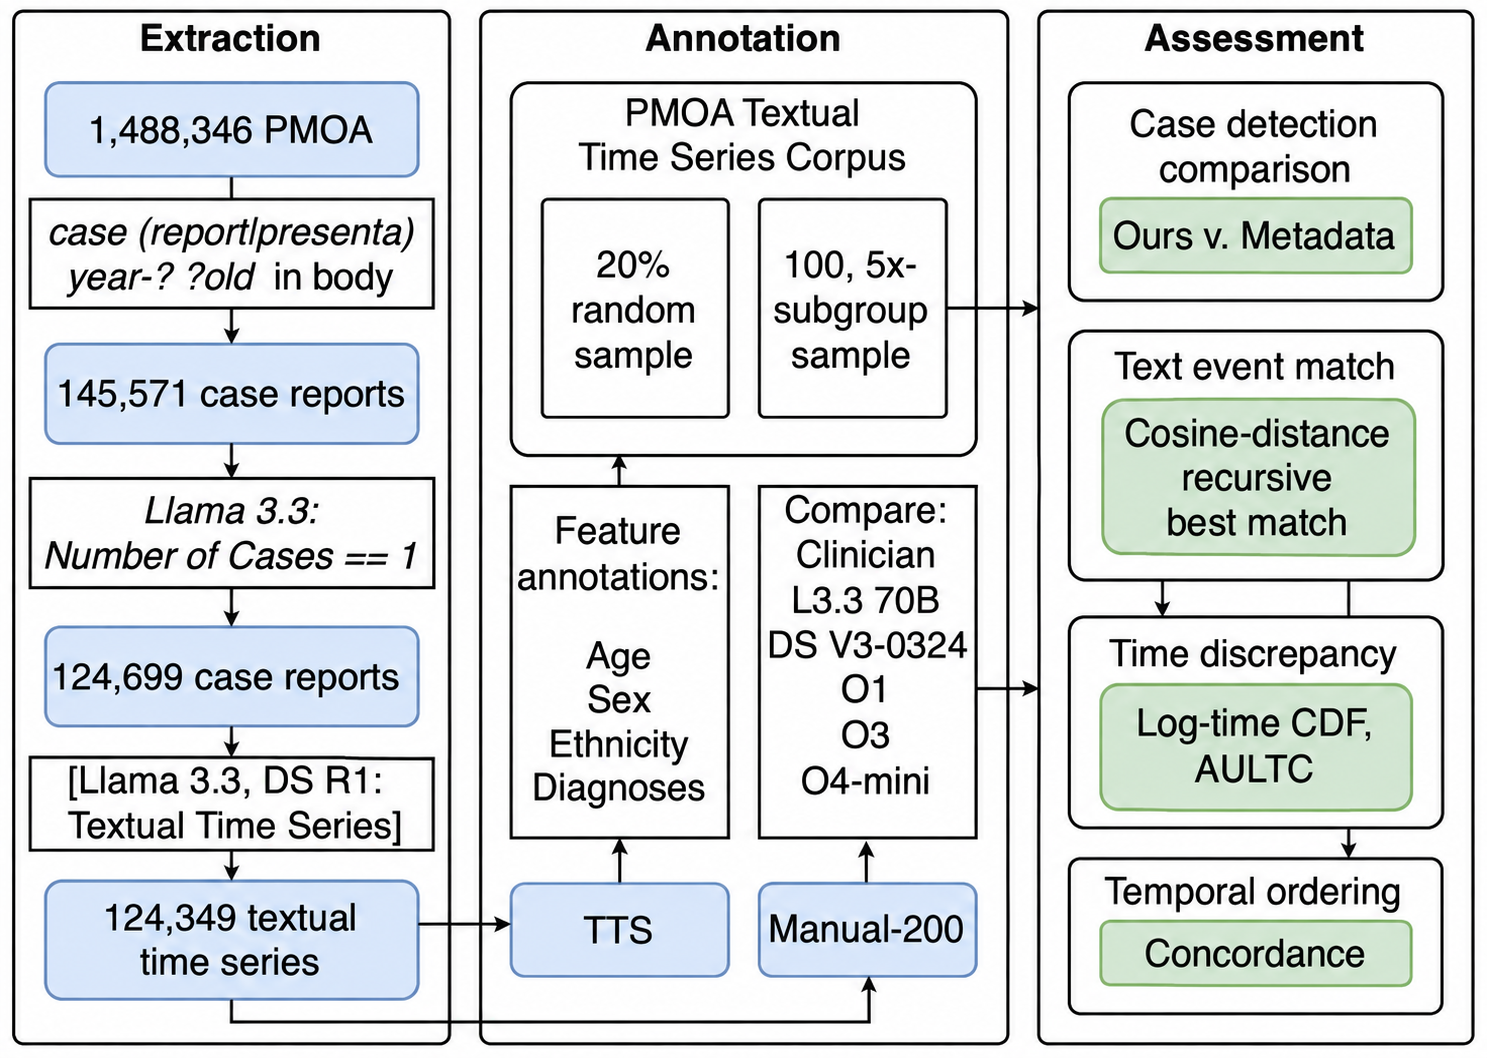
\includegraphics[width=0.75\linewidth]{Chapters/chapter-05/images/Scientific_data/Plots_tables/PMOATTS_flow5_v2.png} % Adjust width
    
    
    

\end{ChFiveFloatBody}
\caption{Flowchart of the extraction and annotation pipeline. The left panel (Extraction) shows how we filtered the PMOA corpus to identify single-patient case reports. The middle panel (Annotation) depicts the generation of textual time series for each case via LLM prompting and the creation of evaluation subsets. The right panel (Assessment) summarizes the evaluation process, including metadata comparison, text event matching, time discrepancy analysis (log-time CDF, AULTC), and temporal order concordance.
    }\ChFiveFloatLabel{ch05:fig:flowchart}
\end{figure}



% !TeX root = ../../../main.tex
\begingroup\raggedright
\subsubsection{Case Report Identification Pipeline}
\label{ch05:sec:case-report-identification-pipeline}

\ChFiveRebuttal{
We obtained the source corpus from the PubMed Central Open Access Subset using the NCBI FTP bulk-download service available at the time of collection. Specifically, we used the 12 plain-text baseline archives in \texttt{oa\_bulk/oa\_noncomm/txt} dated 17 December 2024, with filenames ranging from \texttt{oa\_noncomm\_txt.PMC000xxxxxx.baseline.2024-12-17.tar.gz} to \texttt{oa\_noncomm\_txt.PMC011xxxxxx.baseline.2024-12-17.tar.gz}, downloaded from the then-current endpoint \url{https://ftp.ncbi.nlm.nih.gov/pub/pmc/oa_bulk/oa_noncomm/txt/}. After unpacking the archives, we extracted article content between the ``\texttt{==== Body}'' and ``\texttt{==== Ref}'' markers. Candidate reports were identified using the case-insensitive regular expressions \texttt{case (report|presenta)} and \texttt{year-? ?old}. We then retained documents for which \texttt{Llama 3.3 70B Instruct} returned \texttt{1} to the single-patient case-count prompt. Each released record retains its source PMCID.
}

\ChFiveRebuttal{
The source files were drawn from the non-commercial-use collection of the PMC Open Access Subset. Reuse conditions vary by article and are governed by the license statement attached to each source article; the source PMCID is retained for every PMOA-TTS record to preserve provenance and license traceability.
}

This filter yields 145,571 candidate documents likely to be case reports or case series. 
\ChFiveRebuttal{
The regular expressions serve as deterministic candidate-generation criteria that define the document pool considered for corpus construction; PMOA-TTS does not claim exhaustive retrieval of every possible single-patient case report in PMOA.
}
For the single-patient case-count step, the model is prompted with: ``\texttt{You are a physician. Determine the number of case reports in the following manuscript. Return 0 if it is not a case report. Reply only with the number and nothing else.}'', followed by the document body.
\ChFiveRebuttal{
The pipeline selected 124{,}699 source articles as single-patient case reports. Of these, 124{,}349 produced valid event-time rows. 350 outputs were excluded because they could not be parsed into the required schema.
}
This two-stage process results in a final dataset of \ChFiveRebuttal{124{,}349} single-patient case reports (Figure~\ref{ch05:fig:flowchart}).

We compared our LLM-based case report identification method with PubMed's metadata-based labeling using a carefully designed benchmark.
We created a dataset of 100 reports across five diagnoses—Diabetes, Sepsis, Hypertension, COVID-19, and Atrial Fibrillation—with 10 reports per diagnosis from each method.
A clinician manually reviewed and labeled each report to verify whether it described exactly one case.
\ChFiveRebuttal{
Because this evaluation set was constructed from documents surfaced by at least one of the two identification approaches, recall is computed with respect to manually confirmed single-patient case reports within this evaluation set and should not be interpreted as corpus-level sensitivity over all PMOA documents.
}


%%%%%%%%%%%%%%%%%%%%%%%%%%%%
%%%%%%%%%%%%%%%%%%%%%%%%%%%%

\par\endgroup

% !TeX root = ../../../main.tex
\subsubsection{Timeline Annotation via LLM Prompting}
\label{ch05:sec:timeline-annotation}

\ChFiveHeadingOnly
\paragraph{Textual Time Series (TTS)}
\label{ch05:sec:textual-time-series}

We use large language models (LLMs; \texttt{LLaMA\~3.3\~70B}, \texttt{DeepSeek-R1}) to convert PubMed Open Access (PMOA) case reports into \emph{textual time series} (TTS).
A textual time series is defined as an ordered sequence of clinical event–time pairs, where each event is represented as a short free-text span and each timestamp is a numeric value measured in hours relative to a case-specific reference time.
\ChFiveRebuttal{
The reference event is an anchor for the timeline rather than its boundary. For the LLM extraction, hospital admission is assigned $t=0$ when it is described. If admission is not described, the current clinical presentation that frames the case, such as the main diagnosis or treatment, is assigned $t=0$. Events before and after this reference event receive negative and positive timestamps, respectively. Thus, a phrase such as ``three days before admission'' is represented as $-72$ hours, whereas an event on hospital day 2 is represented as $+24$ hours. Depending on the source report, the resulting TTS may cover an acute encounter or a longitudinal course extending over months or years.
}

In this work, a clinical event refers to any health-related mention that can stand alone semantically and is directly relevant to the patient’s course.
This includes symptoms and signs, diagnoses, procedures and diagnostic tests, treatments and medication administrations, major clinical states, and outcomes.
Explicitly stated pertinent negatives and termination events (such as “no shortness of breath” or “antibiotics discontinued”) are also included. 
Demographic attributes that appear in the narrative, such as age and sex are also extracted as clinical events with reference time (t=0) as the timestamp.
We exclude purely contextual text that does not describe the index patient, such as general background statements or literature discussion.


\ChFiveRebuttal{
PMOA-TTS uses source-faithful, span-based events in the tradition of i2b2 clinical concept annotation, while allowing enough surrounding context for an event to remain clinically interpretable, in contrast to span-based temporal annotation methods (e.g., \cite{sun2013evaluating,uzuner20112010}) and i2b2-style guidelines that often limit events to short prepositional phrases. This is necessary because the timelines include symptoms, findings, procedures, treatments, outcomes, pertinent negatives, uncertainty, and intent in addition to diagnoses. For example, retaining ``pain in chest that radiates substernally'' preserves information that would be lost if the event were reduced to a generic chest-pain code; similarly, retaining ``planned'' distinguishes an intended procedure from one that occurred.
}
Conjunctive mentions are separated into individual events when doing so improves clarity.

Natural-language time expressions are normalized into hour units: coarse expressions such as “hospital day 2” are converted using 24-hour increments from the reference point, interval expressions are represented using the start of the interval, and vague temporal phrases are resolved to approximate offsets that are consistent with narrative ordering and surrounding cues.
The goal of this normalization is to produce a usable relative timeline rather than an exact reconstruction of clock time.

The above specifications define the intended representation of textual time series.
The LLM extraction prompt used in our pipeline (Supplementary Material, Section~\ref{ch05:apd:extraction-prompt}) implements this specification by instructing the model to output a structured sequence of \mbox{(clinical event, time)} tuples.
Events are kept in free-text form to retain clinical specificity rather than being normalized to a fixed ontology.
On average, each case report yields 46 events, and the full corpus comprises over 5.6 million timestamped events, making it the largest publicly available resource of this type in clinical NLP.


\paragraph{Gold Standard Annotations}
\label{ch05:sec:gold-standard-annotations}

We constructed a gold-standard reference set of 200 manually annotated case reports, consisting of 190 cases randomly sampled from PMOA–TTS and 10 cases from our prior pilot study.
All annotations were performed by a single clinical expert following a detailed annotation guideline designed to preserve fidelity to the original narrative while producing event representations suitable for temporal evaluation.

Annotators marked exact text spans corresponding to clinical events without rewriting or paraphrasing, with a small number of controlled exceptions specified in the guideline.
First, conjunctive findings (e.g., “nausea and vomiting”) were permitted to be split into individual events when clinically meaningful.
Second, when needed to supply context, annotators could prepend short clarifying phrases such as “history of” to ensure that extracted events were interpretable as stand-alone findings.
Beyond these two exceptions, events were expected to remain faithful to the wording and granularity of the source text.

To promote consistency, annotators were then instructed to ensure that each event was semantically self-contained (e.g., using “SCC of the lung” rather than “SCC” to avoid ambiguity with other
entities such as cutaneous squamous cell carcinoma or sickle cell crisis).
Related findings were disambiguated when necessary, duplicate mentions of the same event were avoided even when they appeared in multiple sections of a report, and pertinent negative or termination events (e.g., “no shortness of breath” or “denies chest pain”) were included when explicitly stated.
These conventions were applied uniformly across all 200 annotated case reports.

Each annotated event was assigned a timestamp relative to a standardized case reference point.
By definition, this reference point was the time of admission.
If an explicit admission time was not stated, the encounter date (the earliest unambiguous point of primary clinical evaluation within the case narrative) was used as the reference time.
For temporal expressions that described intervals, the start time of the interval was recorded.
All timestamps were expressed in hours relative to the reference time (t=0).

These manually produced timelines serve as the reference standard for evaluating LLM-generated annotations in subsequent sections.


% !TeX root = ../../../main.tex
\subsubsection{Evaluation Metrics}
\label{ch05:sec:evaluation-metrics}

We next assessed the quality of the extracted textual time series using the 200 manually annotated case reports as reference.
Each large language model (LLM) annotator was evaluated across five independent runs to capture run-to-run variation in the generated timelines.
For each model and run, we computed three complementary metrics as described below (detailed description in Supplementary Material, Section \ref{ch05:apd:evaluation-metrics}).

\ChFiveParagraph{Event match rate (recall, precision, and F1)}

To evaluate alignment between predicted and reference clinical events, we applied a recursive best-match strategy adapted from prior work \citep{wang2025large,pmlr-v333-noroozizadeh26a}, as summarized in Algorithm~\ref{ch05:alg:recursive_match}.
At each iteration, the method selects the closest unmatched predicted--reference pair under a text-similarity metric, retains the match if it falls below a distance threshold, and removes both events before continuing.
This procedure yields an efficient one-to-one alignment that accommodates timelines of unequal length.

\ChFiveRebuttal{
We evaluate event identification using event match recall, precision, and F1. Let $M$ denote the number of one-to-one semantic matches after assignment and application of the cosine-distance threshold, $N_{\mathrm{manual}}$ the number of manually annotated events, and $N_{\mathrm{model}}$ the number of model-generated events. Event match recall is defined as $M/N_{\mathrm{manual}}$, event match precision as $M/N_{\mathrm{model}}$, and event match F1 as the harmonic mean of precision and recall. Precision therefore penalizes additional model-generated events that remain unmatched under the one-to-one alignment, complementing recall, which measures the proportion of manually annotated events recovered.
}

As a sensitivity analysis, we also evaluated a globally optimal one-to-one alignment based on the Linear Assignment Problem (LAPJV) \citep{jonker1987shortest}.
Across all models, results differed by at most $0.3$ percentage points in event match recall relative to the recursive heuristic.
We therefore report results using the recursive matching strategy in the main text and provide full LAPJV details and comparison tables in the Supplementary Material (Section~\ref{ch05:apd:lapjv-matching}).


\ChFiveParagraph{Temporal metrics}

We used 2 metrics which evaluate how well the LLM extracts timestamps of clinical events: (a) \textbf{\emph{Temporal concordance}} (c-index) evaluates whether the relative ordering of event times in the model output agrees with the manually annotated timelines, providing an order-based summary of temporal consistency. (b) \textbf{\emph{Log-time discrepancy}} quantifies the absolute difference between the log-transformed timestamps of matched events, and we summarized its distribution using the Area Under the Log-Time CDF (AULTC), which captures the cumulative proportion of events achieving small timing errors. \ChFiveRebuttal{
AULTC is computed over semantically matched event pairs only and therefore measures timestamp accuracy conditional on successful event alignment. Unmatched events do not enter the empirical CDF or AULTC and are evaluated separately by the event-extraction metrics. 
}




% !TeX root = ../../../main.tex
\subsection{Data Records}
\label{ch05:sec:data-records}

\ChFiveRebuttal{
The PMOA-TTS dataset is deposited on Hugging Face \cite{shahriar_noroozizadeh_2026} and is publicly available at \url{https://doi.org/10.57967/hf/10546}.
}
\ChFiveRebuttal{
PMOA-TTS distributes derived structured annotations and source identifiers rather than copies of source-article text, figures, images, or supplementary files. The released annotations and metadata are licensed under CC BY-NC-SA 4.0 (\url{https://creativecommons.org/licenses/by-nc-sa/4.0/}); reuse of the underlying source articles remains subject to the article-level terms displayed by PMC (\url{https://pmc.ncbi.nlm.nih.gov/tools/openftlist/}).
}
The dataset card lists task tags (\texttt{Text Classification}), modality (\texttt{Text}), format support (\texttt{Parquet via auto-conversion}), language (\texttt{English}), and size (``\texttt{100K--1M}'').
Data record schema with an example JSON entry is shown in Figure~\ref{ch05:fig:record_schema}.
% \ChFiveRebuttal{
% The demographic fields are LLM-extracted or LLM-mapped descriptors from the case-report narrative. They should not be interpreted as independently verified biological sex at birth, self-identified race or ethnicity, or population-representative demographic measurements. The model returns Not Specified when no value is identified; ethnicity is Not Specified in 89\% of reports.
% }

\noindent PMOA-TTS has the following dataset splits:

% !TeX root = ../../../main.tex
\begin{figure}[htbp]
\begin{ChFiveFloatBody}

\centering

\begin{minipage}[t]{1\textwidth}
\centering
\footnotesize
\begin{adjustbox}{max width=\linewidth}\begin{tabular}{@{} l l >{\raggedright\arraybackslash}p{4cm} @{}}
\toprule
\textbf{Field} & \textbf{Type} & \textbf{Description} \\
\midrule
\texttt{pmc\_id} & str &
Folder-level ID (PMC000xxxxxx--PMC011xxxxxx). \\

\texttt{case\_report\_id} & str &
Filename of the case (e.g., PMC6417290). \\

\texttt{textual\_timeseries} & List[Dict] &
Sequence of \{"event": str, "time": int\}. \\

\texttt{demographics} & Dict &
\{"age": str/"Not Specified", "sex": str, "ethnicity": str\}. \\

\texttt{diagnoses} & List[str] &
List of diagnosis terms extracted per case. \\

\bottomrule
\end{tabular}\end{adjustbox}
\end{minipage}
\hfill

\begin{minipage}[t]{\linewidth}
\centering
\begin{tcolorbox}[
  colback=gray!5,
  colframe=gray!70,
  title=Example JSON entry,
  boxrule=1pt,
  enhanced,
  %breakable,
  fontupper=\footnotesize
]
\begin{verbatim}
"pmc_id": "PMC006xxxxxx",
"case_report_id": "PMC6417290",

"textual_timeseries": [
  {"event": "56 years old", "time": 0},
  {"event": "male", "time": 0},
  {"event": "HIV-positive", "time": 0},
  {"event": "admitted to the hospital", "time": 0},
  {"event": "knee arthralgia", "time": 0},
  ...
  {"event": "postural headache", "time": 48},
  {"event": "neurological examination", "time": 120},
  {"event": "persistence of headache", "time": 144},
  {"event": "brain computed tomography scan",
   "time": 144},
  ...
  {"event": "symptom free", "time": 4320},
  {"event": "CT scan", "time": 4320},
  {"event": "no brain shift", "time": 4320}
],
"diagnoses": [
  "HIV",
  "Knee arthralgia",
  "Subdural hematoma",
  "Postdural puncture headache (PDPH)"
],
"demographics": {
  "age": 56,
  "sex": "Male",
  "ethnicity": "Not Specified"
}
\end{verbatim}
\end{tcolorbox}
\end{minipage}





\end{ChFiveFloatBody}
\caption{\textbf{top:} PMOA-TTS record schema. \textbf{bottom:} compact example matching the schema above (drawn from our HuggingFace repository (formatted for readability).}\ChFiveFloatLabel{ch05:fig:record_schema}
\end{figure}




\begin{itemize}
    \item \texttt{train\_DSR1/L33}: The full TTS release contains \ChFiveRebuttal{124{,}349 records} with valid event-time rows.
The \texttt{train\_DSR1} and \texttt{train\_L33} splits contain annotations generated using \texttt{DeepSeek-R1} and \texttt{Llama 3.3 70B}, respectively.
Here, a split denotes a version of the dataset defined by the annotation model used.
These splits serve as the default releases and contain the primary annotations used in downstream analyses.
    
    \item {\raggedright \ChFiveRebuttal{\texttt{case\_study\_100} contains the TTS-bearing portion of the 100-document case-identification evaluation. Of the 100 candidate documents reviewed, 88 were confirmed to contain a single-patient case report and therefore have TTS annotations; the remaining 12 did not contain a case report and consequently have no patient timeline in this split.}\par}
    
    \item \texttt{case\_study\_n200}: A benchmark of 200 manually reviewed case reports used for qualitative and quantitative evaluation of LLM-generated annotations.
Each model is evaluated across five independent runs on this subset to assess run-to-run variability in annotation consistency.

\end{itemize}

The data repository also has an additional data split \texttt{TTS\_n200\_additional\_models}, which bundles the single-expert manual timelines (the reference set) together with parallel LLM-generated textual time series for additional models, including open-weight models such as \texttt{DeepSeek-V3}, \texttt{DeepSeek-R1 quantized}, and \texttt{DeepSeek-V3-0324}, and proprietary OpenAI models such as \texttt{GPT5}, \texttt{O1}, \texttt{O3}, and \texttt{O4-mini}.
This split is designed for lightweight benchmarking and cross-model comparison on a fixed 200-case cohort without re-annotating the full corpus.
For the full \ChFiveRebuttal{124{,}349} release, we provide textual time series produced by \texttt{DeepSeek-R1} and \texttt{Llama 3.3 70B}; the additional models are released only on the 200-case subset due to resource constraints.
For completeness, both \texttt{Llama 3.3 70B} and \texttt{DeepSeek-R1} were also executed in five independent runs on the \texttt{case\_study\_n200} subset, and these annotated outputs are included in the dataset.
\ChFiveRebuttal{Additional details regarding exact model versions, access dates, decoding settings, context limits, seeds, and the inference framework are available in Supplementary Material Section  \ref{ch05:sec:supp-model-configuration}}.


% !TeX root = ../../../main.tex
\ChFiveStarSubsection{Data Availability}
\ChFiveRebuttal{
The PMOA-TTS dataset is publicly available on Hugging Face at \url{https://huggingface.co/datasets/snoroozi/pmoa-tts} under the CC BY-NC-SA 4.0 license. The version of record cited in this article is available at \url{https://doi.org/10.57967/hf/10546}. The code used for corpus construction and technical validation is available at \url{https://github.com/jcweiss2/pmoa_tts}.
}



% !TeX root = ../../../main.tex
\ChFiveStarSubsection{Ethics Statement}
% \label{sec:ethics-statement}
\ChFiveRebuttal{
This study is a secondary analysis of publicly available, previously published case reports from the PubMed Central Open Access Subset. No participants were recruited and no non-public clinical records were accessed. The released dataset contains derived structured annotations and source PMCIDs rather than copies of the source articles.
}

%%%%%%%%%%%%%%%%%%%%%%%%%%%%%%%%%%%%%%%%%
%%%%%%%%%%%%%%%% Data Overview
%%%%%%%%%%%%%%%%%%%%%%%%%%%%%%%%%%%%%%%%


% !TeX root = ../../../main.tex
\subsection{Data Overview}
\label{ch05:sec:data-overview}


% !TeX root = ../../../main.tex
\ChFiveHeadingOnly
\subsubsection{Cohort Demographics}
\label{ch05:sec:cohort-demographics}

For demographic extraction, we used an LLM-based query to retrieve age, sex, and ethnicity for each case.
The prompt instructed the model to report age in years; sex as \texttt{Male}, \texttt{Female}, a free-text category, or \texttt{Not Specified}; and ethnicity according to U.S.\ Census categories or \texttt{Not Specified} (full prompt in Supplementary Material, Section~\ref{ch05:apd:demographics-prompt}).
\ChFiveRebuttal{
The demographic fields are LLM-extracted or LLM-mapped descriptors from the case-report narrative. They should not be interpreted as independently verified biological sex at birth, self-identified race or ethnicity, or population-representative demographic measurements.
}

Across PMOA-TTS, the median age is 47 years, with peaks at 5-year intervals, consistent with rounded age reporting in clinical text (Figure~\ref{ch05:fig:demo}).
The distribution of LLM-extracted sex descriptors is approximately balanced (52\% male, 47\% female, 1\% Not Specified).
\ChFiveRebuttal{
Ethnicity was not specified in 89\% of reports. Among reports with an extracted ethnicity category, White/Caucasian and Asian were the most frequent. Given the extensive missingness and the non-population-based nature of case reports, these proportions should not be interpreted as population prevalence or attributed to a specific underlying cause.
}


% !TeX root = ../../../main.tex
\begin{figure}[htbp]
\begin{ChFiveFloatBody}

  \centering
  \begin{minipage}[t]{0.49\linewidth}
    \centering
    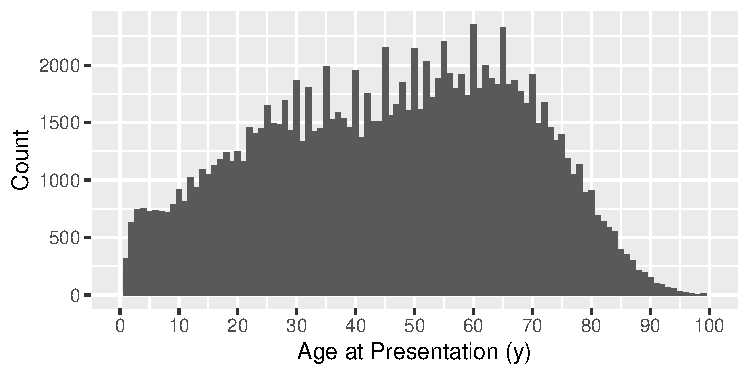
\includegraphics[width=\linewidth]{Chapters/chapter-05/images/Scientific_data/Plots_tables/125k_age.pdf}
  \end{minipage}\hfill
  \begin{minipage}[t]{0.49\linewidth}
    \centering
    \scriptsize
    \begin{tabular}{l r}
      \toprule
      \textbf{Characteristic} & \textbf{Percent (\%)}\\
      \midrule
      \multicolumn{2}{l}{\textbf{Sex}}\\
      \quad Male & 52\\
      \quad Female & 47\\
      \quad Not Specified & 1\\
      \midrule
      \multicolumn{2}{l}{\textbf{Ethnicity}}\\
      \quad White/Caucasian & 5\\
      \quad Asian & 3\\
      \quad African & 1\\
      \quad Other & 2\\
      \quad Not Specified & 89\\
      \bottomrule
    \end{tabular}
  \end{minipage}
  
  
  

\end{ChFiveFloatBody}
\caption{\ChFiveRebuttal{Age distribution and LLM-mapped/extracted demographic descriptors for 124{,}349 PMOA-TTS case reports.}}\ChFiveFloatLabel{ch05:fig:demo}
\end{figure}




% !TeX root = ../../../main.tex
\subsubsection{Descriptive Statistics}
\label{ch05:sec:descriptive-statistics}

The textual time series (TTS) derived from case reports show substantial variation in sequence length and temporal span. 
On average, each TTS contains $46$ timesteps (mean) %\jeremy{mean? median?}, 
with 50\% of sequences comprising between 33 and 57 timesteps (Figure~\ref{ch05:fig:tts_stats}a). 
The length distribution is right-skewed, with a small number of very long trajectories exceeding $1{,}000$ timesteps. 
Events are generally concise: the mean event span is 3.6 words (26.1 characters), and most events fall between two and five words, such as \texttt{“admitted to the hospital”} or \texttt{“CT scan performed”}. 
Longer spans (e.g., $\geq 15$ words) typically correspond to detailed histopathologic or imaging descriptions.

Figure~\ref{ch05:fig:tts_stats}b summarizes the most frequent event strings across the corpus and reflects commonly documented demographic descriptors and clinical milestones (e.g., \texttt{``male''}, \texttt{``female''}, \texttt{``admitted to the hospital''}, \texttt{``discharged''}), as well as prevalent conditions and symptoms (e.g., \texttt{``hypertension''}, \texttt{``fever''}, \texttt{``vomiting''}). 
Importantly, these counts are computed from the \emph{event strings in the TTS} and therefore capture only information that is explicitly stated and extracted as an event in the narrative. 
\ChFiveRebuttal{The demographic percentages in Section~\ref{ch05:sec:cohort-demographics} are patient-level outputs from the dedicated demographic extraction, with one demographic record per report. In contrast, Figure \ref{ch05:fig:tts_stats}b counts literal event strings in the TTS - 57,394 occurrences of male and 52,437 occurrences of female, which do not sum to the total number of case reports in our corpus (n = 124,349). This is because some reports ($14\%$) do not explicitly state sex in a way that is extracted as an event.}
% As a result, demographic events such as \texttt{``male''} and \texttt{``female''} need not sum to the total number of case reports (124k), because some reports ($14\%$) do not explicitly state sex in a way that is extracted as an event.
%even when a separate demographic field may be populated by an auxiliary extraction step.


The temporal coverage of individual case reports also varies widely. 
The mean case duration is 415.9 days (median 104.0 days), with half of cases spanning between 28 and 391 days and the 99th percentile extending to 4{,}380 days (12 years). 
On average, 77.6\% of events share timestamps with at least one other event, indicating frequent temporal co-occurrence within a report. 
The median uniqueness ratio of event timestamps is 0.14, reflecting the common practice of documenting multiple events at the same recorded time (e.g., grouped laboratory results or procedure bundles). 
Approximately 17\% of events have negative timestamps, representing history prior to the chosen reference point (typically admission), such as past diagnoses or prior treatments.
Together, these statistics summarize the density and temporal heterogeneity of clinical event sequences across PMOA-TTS. 

% \vspace{-5mm}

% !TeX root = ../../../main.tex
\begin{figure}[htbp]
\begin{ChFiveFloatBody}

    \centering
    \begin{minipage}{0.48\textwidth}
        \centering
        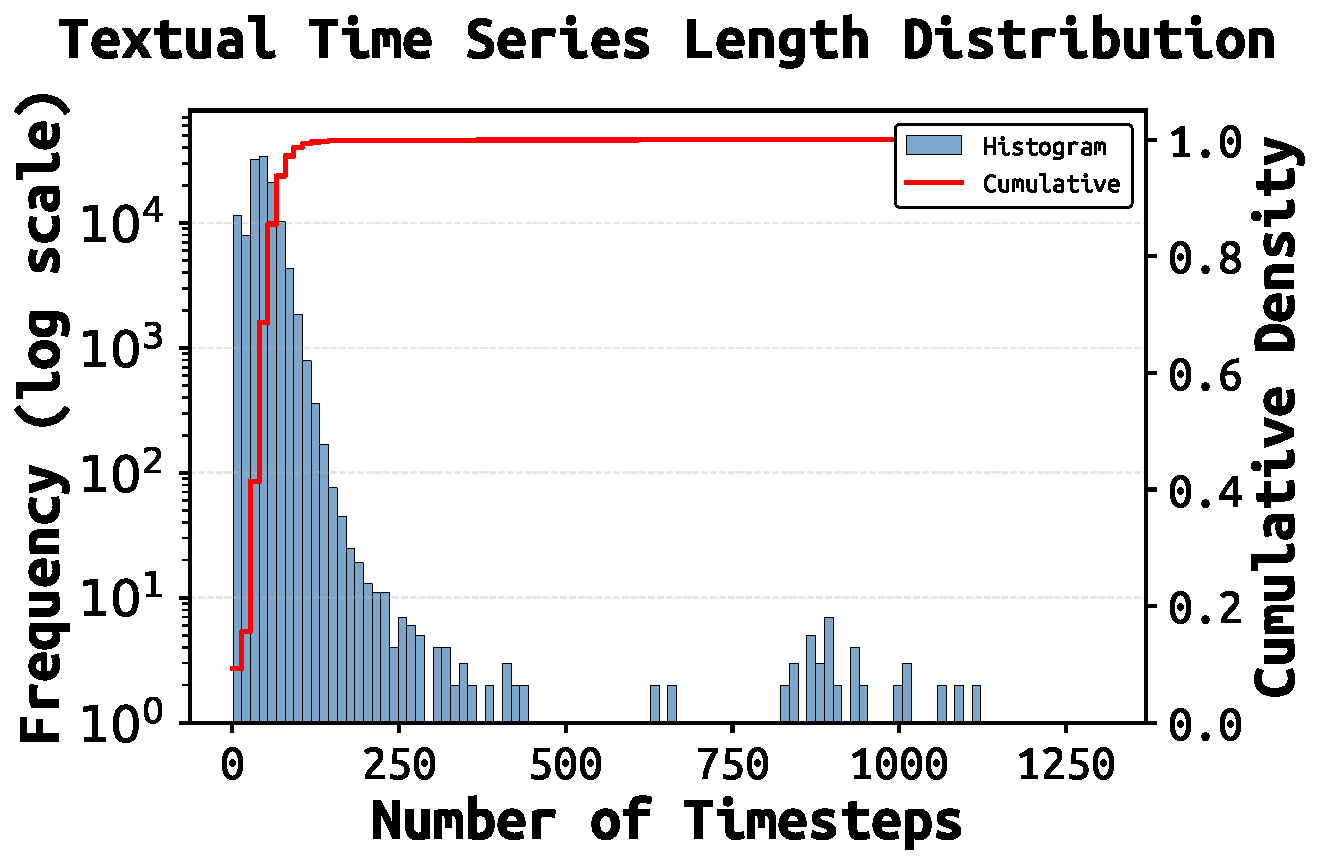
\includegraphics[width=\linewidth]{Chapters/chapter-05/images/Scientific_data/Plots_tables/tts_length_distribution.pdf}
        \ChFivePanelText{(a) Distribution of time series lengths (timesteps) across the dataset.}
    \end{minipage}\hfill
    \begin{minipage}{0.48\textwidth}
        \centering
        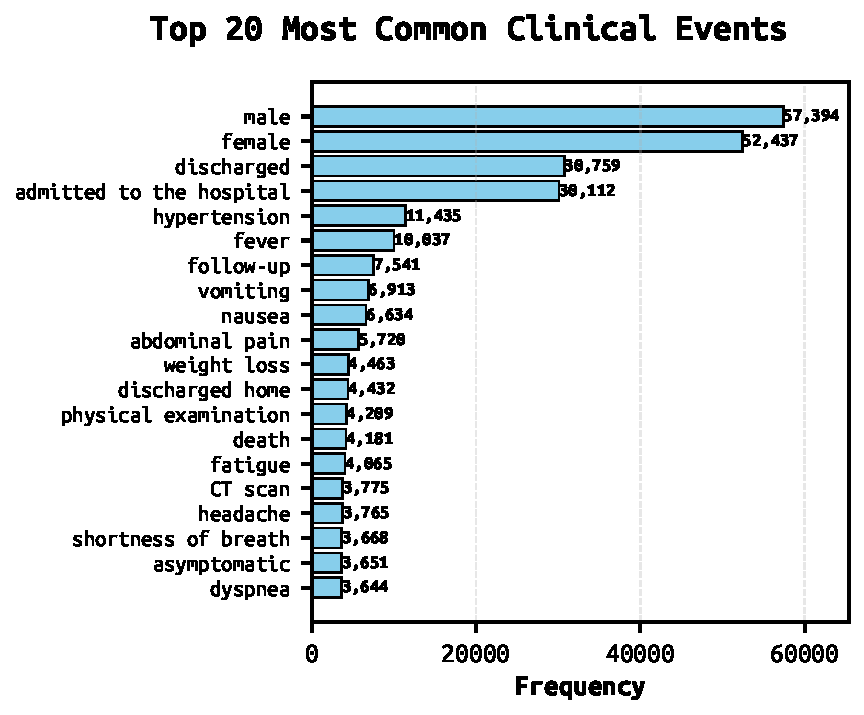
\includegraphics[width=\linewidth]{Chapters/chapter-05/images/Scientific_data/Plots_tables/top_20_common_events.pdf}
        \ChFivePanelText{(b) Most frequently occurring events across all case reports.
        }
    \end{minipage}
    
    
    % \vspace{-7.5mm}

\end{ChFiveFloatBody}
\caption{Overview of textual time series characteristics in PMOA-TTS.}\ChFiveFloatLabel{ch05:fig:tts_stats}
\end{figure}



% !TeX root = ../../../main.tex
\subsubsection{Diagnosis Distribution Analysis}
\label{ch05:diagnosis-distribution-analysis}

To characterize diagnostic coverage, we prompted the LLM to act as an expert physician and list patient-specific diagnoses for each case report. 
The prompt asked the model to extract final diagnostic labels (e.g., ``acne'', ``DRESS syndrome'') rather than isolated clinical findings (e.g., ``rash'', ``leukocytosis''), to place the primary diagnosis first, and to output one diagnosis per line without explanatory text (full prompt in Supplementary Material, Section~\ref{ch05:apd:diagnosis-prompt}).

Free-text diagnoses were then standardized to the Unified Medical Language System (UMLS) using the ScispaCy entity linker (\texttt{en\_core\_sci\_lg}) with the UMLS knowledge base. 
\ChFiveRebuttal{
Each complete extracted diagnosis string was supplied directly to the UMLS candidate generator, with candidate selection designed to avoid fragmentation and improve canonical concept assignment (Supplementary Material, Section~\ref{ch05:apd:umls-mapping}).
}

Figure~\ref{ch05:fig:top_diagnoses} shows the 20 most frequent UMLS-normalized diagnoses in PMOA-TTS.
These are dominated by common cardiometabolic and renal conditions, including hypertensive disease, diabetes mellitus and its subtypes, coronary artery disease, dyslipidemia, and chronic kidney disease.
\ChFiveRebuttal{
Figure~\ref{ch05:fig:diagnoses} characterizes diagnoses represented within PMOA-TTS; it is not an evaluation of diagnostic recognition. Common diagnoses may appear as comorbidities in reports whose primary focus is a rare or atypical presentation.
}

We further examined co-occurrence structure using a clustered heatmap of diagnosis pairs (Figure~\ref{ch05:fig:diagnosis_cooccurrence}).
The heatmap reveals coherent groupings among related conditions, most notably across diabetes variants, as well as broader co-occurrence patterns among cardiovascular, metabolic, and renal diagnoses.
These patterns are consistent with well-established comorbidity relationships (e.g., hypertension with diabetes, or atrial fibrillation with coronary artery disease) and illustrate how the corpus captures clinically meaningful disease constellations.

\ChFiveRebuttal{
To characterize rare-disease representation more directly, we matched UMLS CUIs associated with extracted diagnoses against disorder-level entities in the Orphanet rare-disease nomenclature \citep{lucano2026orphanet} using exact, validated UMLS mappings. After excluding groups and subtypes of disorders and entities designated as inactive, historical, deprecated, obsolete, or non-rare, the reference contained 5,942 Orphanet disorders. Overall, 41{,}775 of 124{,}349 reports (33.6\%) contained at least one extracted diagnosis mapped to an eligible Orphanet disorder, spanning 2,426 distinct ORPHAcodes. Across all extracted diagnoses, 50,299 of 474,075 mappings (10.6\%) matched the Orphanet reference. These statistics characterize rare-disease representation within PMOA-TTS rather than population prevalence.
}


% !TeX root = ../../../main.tex
\begin{figure}[htbp]
\begin{ChFiveFloatBody}

    \centering
    \subfloat[{Most frequent diagnoses.}]{\begin{minipage}[t]{0.39\textwidth}
        \centering
        \raisebox{40pt}{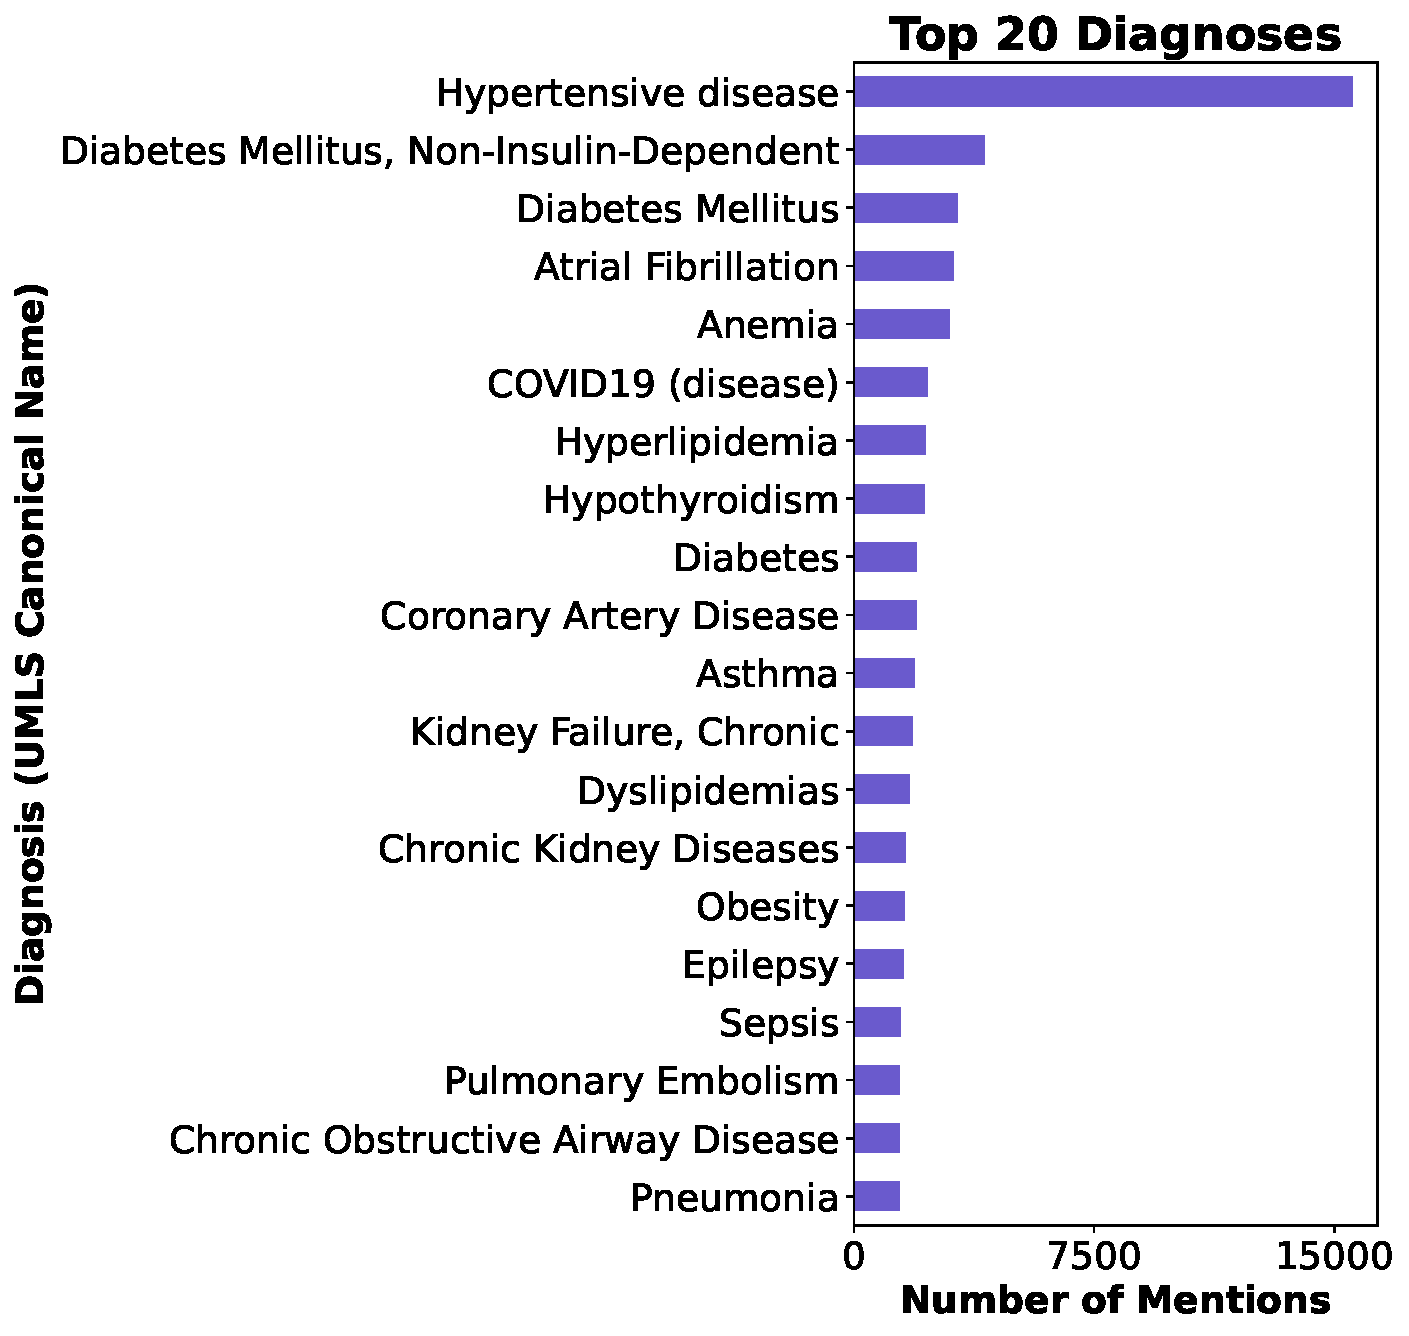
\includegraphics[width=0.99\linewidth]{Chapters/chapter-05/images/Scientific_data/Plots_tables/top_diagnoses_umls_corrected_lexical_tiebreak_paper_ready.pdf}}
        
        \label{ch05:fig:top_diagnoses}
    \end{minipage}}
    \hfill
    \subfloat[{Diagnosis co-occurrence heatmap.}]{\begin{minipage}[t]{0.6\textwidth}
        \centering
        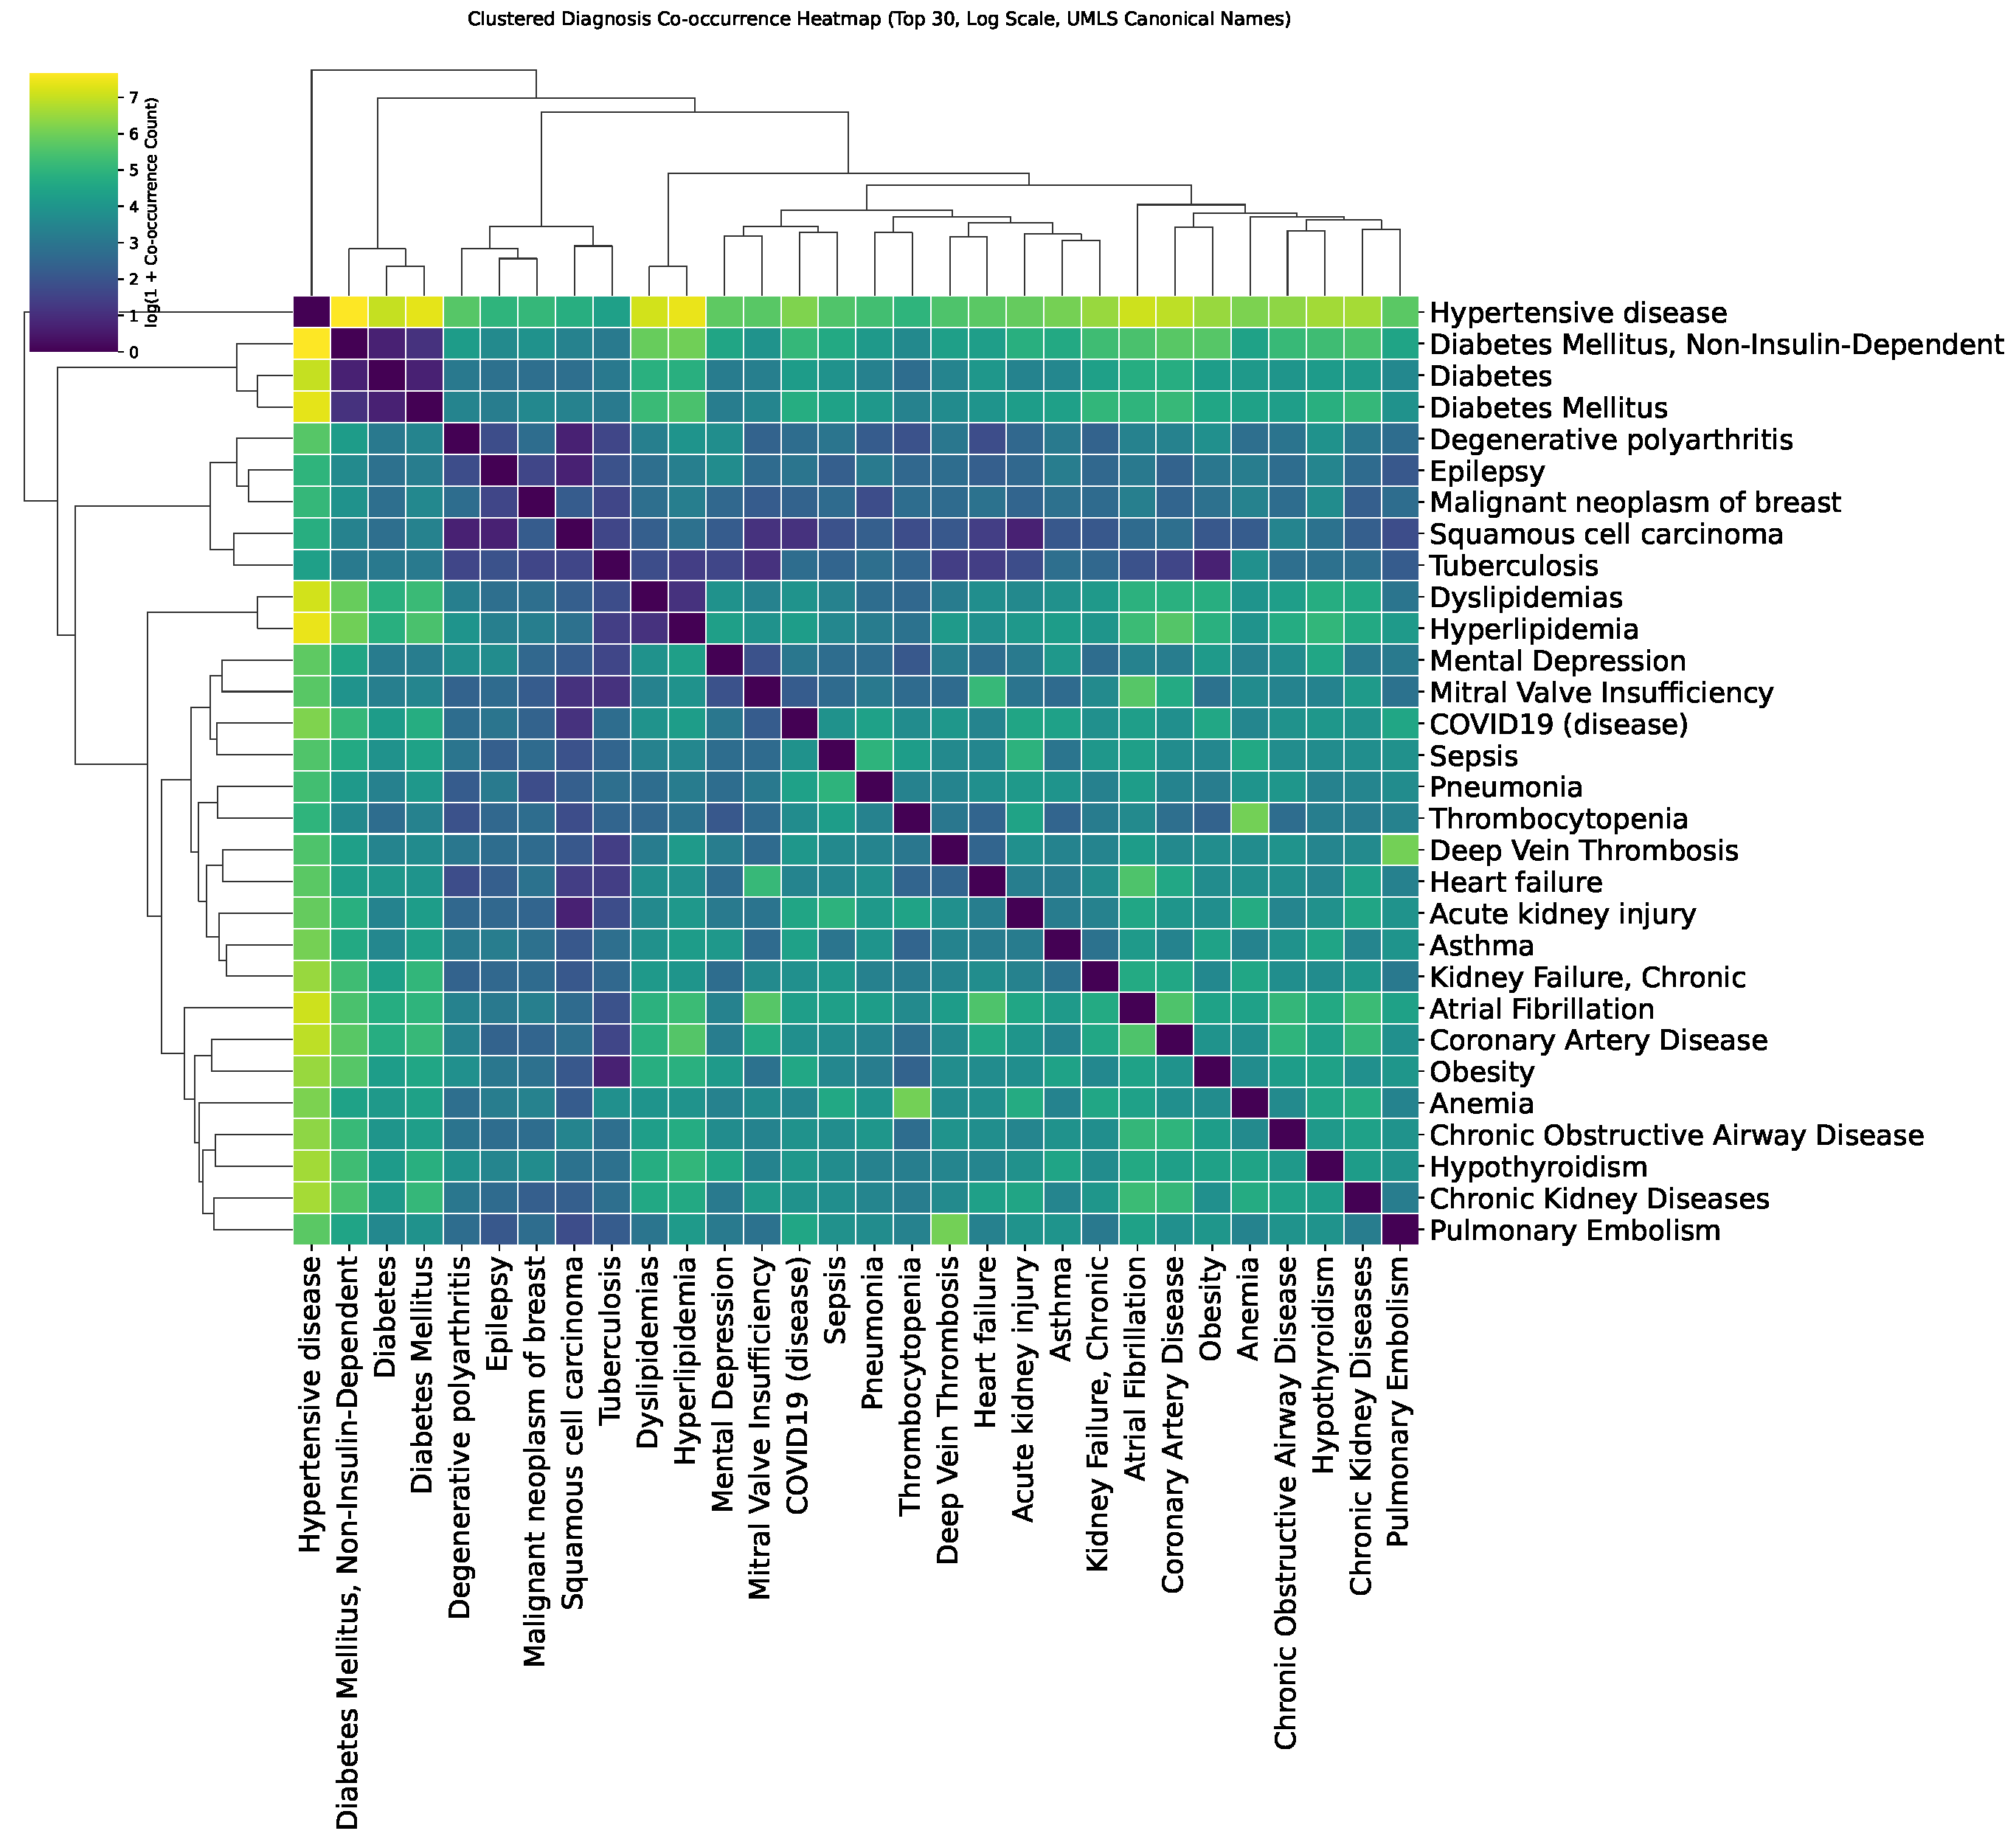
\includegraphics[width=0.99\linewidth]{Chapters/chapter-05/images/Scientific_data/Plots_tables/clustered_cooccurrence_heatmap_top30_corrected_lexical_tiebreak_canonical.pdf}
        
        \label{ch05:fig:diagnosis_cooccurrence}
    \end{minipage}}
    
    
    

\end{ChFiveFloatBody}
\caption{Frequency and co-occurrence patterns of UMLS-normalized diagnoses in PMOA-TTS. (a) The 20 most frequently mentioned diagnoses using canonical UMLS names. (b) Pairwise diagnosis co-occurrence (log-transformed counts) with hierarchical clustering, highlighting groups of frequently co-mentioned conditions.}\ChFiveFloatLabel{ch05:fig:diagnoses}
\end{figure}






% !TeX root = ../../../main.tex
\subsection{Technical Validation}
\label{ch05:sec:technical-validation}


% !TeX root = ../../../main.tex
\ChFiveHeadingOnly
\subsubsection{Case Report Identification Performance}
\label{ch05:sec:case-report-identification-performance}


% !TeX root = ../../../main.tex
\begin{table}[htbp]
\caption{\ChFiveRebuttal{Case-report identification performance by diagnosis and in aggregate on the manually reviewed 100-document evaluation set. Recall is calculated with respect to confirmed single-patient case reports within this evaluation set.}}\ChFiveFloatLabel{ch05:tab:case_report_identification}
\ChFiveTableBodyStart
\begin{ChFiveFloatBody}

\footnotesize
\centering


\begin{tabular}{llcccc}
\toprule
Subset & Diagnosis & Precision & Recall & Accuracy & F1 Score \\
\midrule
\multirow{6}{*}{PubMed metadata} 
    & Atrial Fibrillation & 0.84 & 0.94 & 0.80 & 0.89 \\
    & COVID-19            & 0.94 & 0.89 & 0.85 & 0.92 \\
    & Diabetes            & 0.85 & 1.00 & 0.85 & 0.92 \\
    & Hypertension        & 1.00 & 1.00 & 1.00 & 1.00 \\
    & Sepsis              & 0.95 & 0.95 & 0.90 & 0.95 \\
\cmidrule(lr){2-6}
    & \textbf{All Diagnoses} & \text{0.92} & \textbf{0.96} & \text{0.88} & \text{0.94} \\
\midrule
\multirow{6}{*}{LLM-Pipeline}
    & Atrial Fibrillation & 1.00 & 1.00 & 1.00 & 1.00 \\
    & COVID-19            & 1.00 & 0.89 & 0.90 & 0.94 \\
    & Diabetes            & 1.00 & 0.94 & 0.95 & 0.97 \\
    & Hypertension        & 1.00 & 0.95 & 0.95 & 0.97 \\
    & Sepsis              & 1.00 & 1.00 & 1.00 & 1.00 \\
\cmidrule(lr){2-6}
    & \textbf{All Diagnoses} & \textbf{1.00} & \textbf{0.96} & \textbf{0.96} & \textbf{0.98} \\
\bottomrule
\end{tabular}


\end{ChFiveFloatBody}
\end{table}






Table~\ref{ch05:tab:case_report_identification} reports the performance of the LLM-based pipeline and a PubMed metadata filter for identifying single-patient case reports on the manually reviewed 100-document case-identification evaluation set, evaluated across five diagnostic categories using clinician-assigned labels as reference.
In this evaluation set, the LLM-based pipeline achieved precision of 1.00 across all diagnostic categories and in aggregate, meaning that every document flagged as a single-patient case report by the pipeline was confirmed as such in this sample.
The PubMed metadata filter showed lower and more variable precision, ranging from 0.84 (atrial fibrillation) to 1.00 (hypertension), with an overall precision of 0.92. 
\ChFiveRebuttal{
Within the manually reviewed evaluation set, both methods achieved recall of 0.96, indicating comparable coverage of the confirmed single-patient case reports represented in this set. This quantity is not an estimate of corpus-level sensitivity.
}

Overall accuracy was higher for the LLM-based pipeline (0.96 vs.\ 0.88), largely due to better exclusion of multi-patient or non-case-report articles that were sometimes misclassified by the metadata-based filter.
Performance patterns were consistent across diagnostic subsets, with the LLM pipeline maintaining high F1 scores (0.94--1.00). 
\ChFiveRebuttal{
These results characterize identification performance within the manually reviewed evaluation set; because the set contains documents surfaced by at least one of the two approaches, they do not establish corpus-level sensitivity over PMOA.
}


% !TeX root = ../../../main.tex
\subsubsection{Evaluation of Clinical Textual Time Series Quality}
\label{ch05:sec:evaluation-of-tts-quality}

Using the 200 manually annotated case reports as reference, we evaluated textual time series quality across LLM annotators and runs using event match recall, precision, and F1, temporal concordance (c-index), and AULTC. Table~\ref{ch05:tab:model_comparison} reports mean and standard deviation across runs for seven LLM variants: \texttt{Llama 3.3 70B}, \texttt{DeepSeek-R1}, \texttt{DeepSeek-V3}, \texttt{OpenAI GPT-5}, \texttt{OpenAI O4-mini}, \texttt{OpenAI O3}, and \texttt{OpenAI O1}.

\ChFiveRebuttal{
We additionally evaluated event match precision and F1 to account for model-generated events that were not matched to the manually annotated timeline (Tables~\ref{ch05:tab:model_comparison} and~\ref{ch05:tab:bootstrap_intervals}). Precision varied from 0.756 for GPT-5 to 0.873 for O1, while recall showed the opposite pattern for these models (0.845 for GPT-5 versus 0.637 for O1), illustrating differences in the precision--recall tradeoff across models. F1 ranged from 0.712 to 0.798. Bootstrap 95\% confidence intervals for precision and F1 are reported in Table~\ref{ch05:tab:bootstrap_intervals}. Table~\ref{ch05:tab:model_comparison_lapjv} also includes precision and F1 under the LAPJV-based matching analysis.
}



% !TeX root = ../../../main.tex
\begin{table}[htbp]
\caption{\ChFiveRebuttal{Comparison of models on Event Match Rate (Recall), Event Match Precision, Event Match F1, Concordance, and AULTC with respect to 200 manually annotated case reports across 5 independent runs for each model.}}\ChFiveFloatLabel{ch05:tab:model_comparison}
\ChFiveTableBodyStart
\begin{ChFiveFloatBody}


\footnotesize
\centering
\setlength{\tabcolsep}{3pt}


\begin{tabular}{lccccc}
\hline
\textbf{Model} &
\begin{tabular}{c}\textbf{Event Match}\\\textbf{ Recall}\end{tabular} &
\begin{tabular}{c}\textbf{Event Match}\\\textbf{Precision}\end{tabular} &
\begin{tabular}{c}\textbf{Event Match}\\\textbf{F1}\end{tabular} &
\textbf{Concordance} &
\textbf{AULTC} \\
\hline
\texttt{Llama 3.3 70B}
& 0.673 $\pm$ 0.003
& 0.757 $\pm$ 0.036
& 0.712 $\pm$ 0.015
& 0.846 $\pm$ 0.002
& 0.721 $\pm$ 0.001 \\

\texttt{DeepSeek-R1}
& 0.746 $\pm$ 0.008
& 0.788 $\pm$ 0.006
& 0.766 $\pm$ 0.005
& 0.773 $\pm$ 0.010
& 0.728 $\pm$ 0.004 \\

\texttt{DeepSeek-V3}
& 0.760 $\pm$ 0.004
& 0.796 $\pm$ 0.006
& 0.778 $\pm$ 0.004
& 0.783 $\pm$ 0.007
& 0.731 $\pm$ 0.002 \\

\texttt{OpenAI GPT-5}
& \textbf{0.845 $\pm$ 0.005}
& 0.756 $\pm$ 0.007
& \textbf{0.798 $\pm$ 0.003}
& \textbf{0.902 $\pm$ 0.002}
& 0.722 $\pm$ 0.001 \\

\texttt{OpenAI O4-mini}
& 0.748 $\pm$ 0.019
& 0.814 $\pm$ 0.015
& 0.779 $\pm$ 0.017
& 0.846 $\pm$ 0.006
& \textbf{0.750 $\pm$ 0.002} \\

\texttt{OpenAI O3}
& 0.733 $\pm$ 0.003
& 0.837 $\pm$ 0.003
& 0.782 $\pm$ 0.002
& 0.898 $\pm$ 0.002
& 0.737 $\pm$ 0.003 \\

\texttt{OpenAI O1}
& 0.637 $\pm$ 0.007
& \textbf{0.873 $\pm$ 0.003}
& 0.737 $\pm$ 0.005
& 0.885 $\pm$ 0.002
& 0.732 $\pm$ 0.002 \\
\hline
\end{tabular}


\end{ChFiveFloatBody}
\end{table}




% !TeX root = ../../../main.tex
\begin{table}[htbp]
\caption{\ChFiveRebuttal{Bootstrap 95\% confidence intervals for Event Match Rate (Recall), Event Match Precision, Event Match F1, Concordance, and AULTC across models evaluated on the 200 manually annotated case reports.}}\ChFiveFloatLabel{ch05:tab:bootstrap_intervals}
\ChFiveTableBodyStart
\begin{ChFiveFloatBody}


\footnotesize
\centering
\setlength{\tabcolsep}{3pt}


\begin{tabular}{lccccc}
\hline
\textbf{Model} &
\begin{tabular}{c}\textbf{Event Match}\\\textbf{Recall}\end{tabular} &
\begin{tabular}{c}\textbf{Event Match}\\\textbf{Precision}\end{tabular} &
\begin{tabular}{c}\textbf{Event Match}\\\textbf{F1}\end{tabular} &
\textbf{Concordance} &
\textbf{AULTC} \\
&
\textbf{(95\% CI)} &
\textbf{(95\% CI)} &
\textbf{(95\% CI)} &
\textbf{(95\% CI)} &
\textbf{(95\% CI)} \\
\hline
\texttt{Llama 3.3 70B}
& [0.647, 0.715]
& [0.564, 0.835]
& [0.603, 0.770]
& [0.819, 0.864]
& [0.698, 0.746] \\

\texttt{DeepSeek-R1}
& [0.702, 0.771]
& [0.760, 0.807]
& [0.730, 0.789]
& [0.747, 0.782]
& [0.707, 0.751] \\

\texttt{DeepSeek-V3}
& [0.736, 0.795]
& [0.782, 0.825]
& [0.758, 0.810]
& [0.756, 0.813]
& [0.708, 0.753] \\

\texttt{OpenAI GPT-5}
& [0.812, 0.866]
& [0.751, 0.792]
& [0.780, 0.827]
& [0.889, 0.911]
& [0.702, 0.745] \\

\texttt{OpenAI O4-mini}
& [0.695, 0.764]
& [0.772, 0.828]
& [0.732, 0.795]
& [0.824, 0.868]
& [0.727, 0.772] \\

\texttt{OpenAI O3}
& [0.703, 0.765]
& [0.818, 0.855]
& [0.756, 0.808]
& [0.880, 0.915]
& [0.721, 0.761] \\

\texttt{OpenAI O1}
& [0.612, 0.686]
& [0.864, 0.890]
& [0.717, 0.775]
& [0.869, 0.900]
& [0.712, 0.753] \\
\hline
\end{tabular}


\end{ChFiveFloatBody}
\end{table}



To quantify uncertainty from a complementary perspective, we also performed a bootstrap analysis based on resampling the 200 annotated cases with replacement and recomputing metrics to obtain 95\% confidence intervals. These intervals characterize variability arising from the composition of the reference set, whereas the across-run standard deviations reflect variability in model sampling. The full set of bootstrap intervals is reported in Table~\ref{ch05:tab:bootstrap_intervals}.

% \begin{figure}[!tbp]
% \centering
%     \begin{minipage}[t]{0.242\textwidth}
%     \centering
%     \includegraphics[page=1, width=\linewidth]{Plots_tables/pmoa_updated_man_figs.pdf}
%     \end{minipage}
%     \hfill
%     \begin{minipage}[t]{0.242\textwidth}
%     \centering
%     \includegraphics[page=2, width=\linewidth]{Plots_tables/pmoa_updated_man_figs.pdf}
%     \end{minipage}
%     \hfill
%     \begin{minipage}[t]{0.242\textwidth}
%     \centering
%     \includegraphics[page=3, width=\linewidth]{Plots_tables/pmoa_updated_man_figs.pdf}
%     \end{minipage}
%     \hfill
%     \begin{minipage}[t]{0.242\textwidth}
%     \centering
%     \includegraphics[page=4, width=\linewidth]{Plots_tables/pmoa_updated_man_figs.pdf}
%     \end{minipage}
%     \caption{Comparison of different LLM for extracting temporal clinical events from case reports. From left to right: (\textbf{A}) event match cumulative distribution function, (\textbf{B}) concordance box plots, (\textbf{C}) time discrepancy from manual annotation timestamps among matched events (overall), and (\textbf{D}) time discrepancy disaggregated by clinician annotator timestamp (time from presentation). 
%     %\textcolor{red}{Have same figure for LAPJV?}
%     }
%     \label{fig:tts_evaluation}
%     \vspace{-10pt}
% \end{figure}




% !TeX root = ../../../main.tex
\begin{figure}[htbp]
\begin{ChFiveFloatBody}

\centering

% First row: panels A and B
\begin{minipage}[t]{0.49\linewidth}
    \centering
    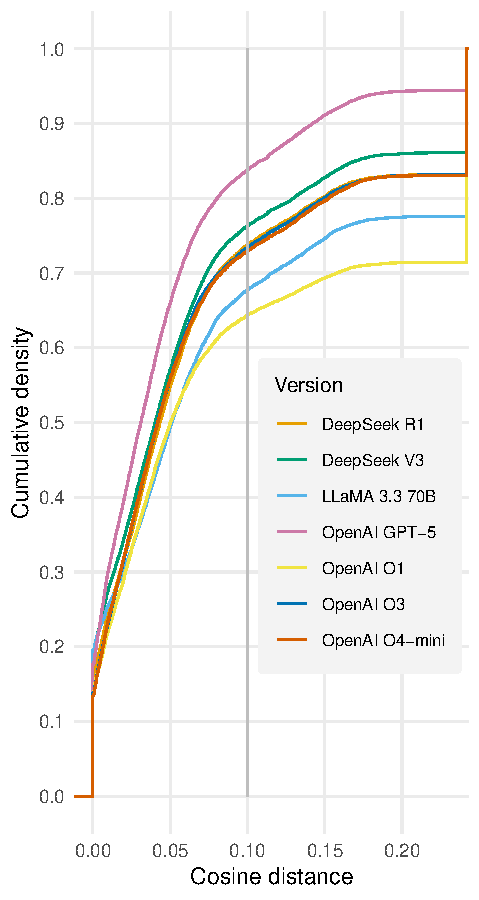
\includegraphics[
        page=1,
        width=0.8\linewidth
    ]{Chapters/chapter-05/images/Plots_tables/pmoa_updated_man_figs.pdf}
\end{minipage}
\hfill
\begin{minipage}[t]{0.49\linewidth}
    \centering
    \includegraphics[
        page=2,
        width=0.8\linewidth
    ]{Chapters/chapter-05/images/Plots_tables/pmoa_updated_man_figs.pdf}
\end{minipage}

\par\medskip

% Second row: panels C and D
\begin{minipage}[t]{0.49\linewidth}
    \centering
    \includegraphics[
        page=3,
        width=0.8\linewidth
    ]{Chapters/chapter-05/images/Plots_tables/pmoa_updated_man_figs.pdf}
\end{minipage}
\hfill
\begin{minipage}[t]{0.49\linewidth}
    \centering
    \includegraphics[
        page=4,
        width=0.8\linewidth
    ]{Chapters/chapter-05/images/Plots_tables/pmoa_updated_man_figs.pdf}
\end{minipage}





\end{ChFiveFloatBody}
\caption{
Comparison of different LLMs for extracting temporal clinical events
from case reports:
(\textbf{A}) cumulative distribution of event-matching cosine distances;
(\textbf{B}) temporal-concordance box plots;
(\textbf{C}) timestamp discrepancies between model-generated and manual
annotations among semantically matched events; and
(\textbf{D}) timestamp discrepancies stratified by the clinician-annotated
time relative to presentation.
}\ChFiveFloatLabel{ch05:fig:tts_evaluation}
\end{figure}



\paragraph{Text Event Match Performance}
\label{ch05:sec:text-event-match-performance}
Figure~\ref{ch05:fig:tts_evaluation} (A) shows the cumulative distributions of cosine distances between model-generated and reference event descriptions, with a threshold of 0.1 used to define a successful semantic match. At this threshold, 
\ChFiveRebuttal{
\texttt{GPT-5} had the highest mean event-recall point estimate (0.845), followed by \texttt{DeepSeek-V3} (0.760), \texttt{O4-mini} (0.748), and \texttt{DeepSeek-R1} (0.746). \texttt{O3} and \texttt{Llama 3.3 70B} had mean recall values of 0.733 and 0.673, respectively, while \texttt{O1} had the lowest mean recall (0.637). These point estimates show variation across models in the proportion of manually annotated clinical events recovered under the selected semantic-matching threshold.
}
% \ChFiveRebuttal{
% \texttt{GPT-5} achieved the highest mean event recall (0.845), followed by \texttt{DeepSeek-V3} (0.760), \texttt{O4-mini} (0.748), and \texttt{DeepSeek-R1} (0.746). \texttt{O3} and \texttt{Llama 3.3 70B} achieved lower recall of 0.733 and 0.673, respectively, while \texttt{O1} had the lowest recall (0.637). These results indicate meaningful differences across models in the proportion of manually annotated clinical events recovered under the selected semantic-matching threshold.
% }

\paragraph{Temporal Ordering Performance}
\label{ch05:sec:temporal-ordering-performance}

Using the same similarity threshold to identify matched events, temporal ordering accuracy was evaluated with the concordance index (c-index). As shown in Figure~\ref{ch05:fig:tts_evaluation} (B),
\ChFiveRebuttal{
\texttt{GPT-5} had the highest mean concordance point estimate (0.902), followed closely by \texttt{O3} (0.898) and \texttt{O1} (0.885). \texttt{Llama 3.3 70B} and \texttt{O4-mini} both had mean concordance of 0.846, while \texttt{DeepSeek-V3} and \texttt{DeepSeek-R1} had mean concordance of 0.783 and 0.773, respectively. However, the bootstrap 95\% confidence intervals for the leading models overlapped. We therefore interpret the ordering of the mean estimates descriptively and do not consider these results evidence that one model was statistically superior in temporal ordering.
The differences between event recall and concordance across models illustrate that these metrics capture distinct aspects of timeline quality. For example, \texttt{O1} had the lowest event recall but relatively high concordance among the events that were successfully matched.
}
% \ChFiveRebuttal{\texttt{GPT-5} achieved the highest mean concordance (0.902), closely followed by \texttt{O3} (0.898) and \texttt{O1} (0.885). \texttt{Llama 3.3 70B} and \texttt{O4-mini} both achieved concordance of 0.846, while \texttt{DeepSeek-V3} and \texttt{DeepSeek-R1} had lower concordance of 0.783 and 0.773, respectively. The differences between event recall and concordance across models illustrate that event recovery and temporal ordering capture distinct aspects of timeline quality. For example, \texttt{O1} had the lowest event recall but relatively high concordance among the events that were successfully matched.}
This contrast highlights that models that align fewer but clearer events may achieve high ordering scores, whereas models with broader coverage face a more challenging ordering task.


\paragraph{Time Discrepancy Analysis}
\label{ch05:sec:time-descrepancy-analysis}
Figure~\ref{ch05:fig:tts_evaluation} (C, D) presents cumulative distributions of log-scaled time discrepancies between predicted and reference timestamps for semantically matched events. 
\ChFiveRebuttal{
\texttt{O4-mini} had the highest mean AULTC point estimate (0.750), followed by \texttt{O3} (0.737). \texttt{O1}, \texttt{DeepSeek-V3}, and \texttt{DeepSeek-R1} had similar intermediate mean values of 0.732, 0.731, and 0.728, respectively, while \texttt{GPT-5} (0.722) and \texttt{Llama 3.3 70B} (0.721) had the lowest mean AULTC values. However, the bootstrap 95\% confidence intervals overlapped across several models. We therefore treat this ordering as descriptive and do not interpret the higher mean for \texttt{O4-mini} as evidence of statistically distinct superiority in timestamp accuracy.
The variation in mean AULTC was smaller than the variation observed for event recall and temporal concordance. The interval-stratified analysis in Figure~\ref{ch05:fig:tts_evaluation} (D) further shows how timestamp accuracy varies with temporal distance from the admission reference time.
}
% \ChFiveRebuttal{
% \texttt{O4-mini} achieved the highest mean AULTC (0.750), followed by \texttt{O3} (0.737). \texttt{O1}, \texttt{DeepSeek-V3}, and \texttt{DeepSeek-R1} achieved similar intermediate values of 0.732, 0.731, and 0.728, respectively, while \texttt{GPT-5} (0.722) and \texttt{Llama 3.3 70B} (0.721) had the lowest mean AULTC values. 
% Notably, the spread in AULTC performance is less pronounced than that observed for the event match rate and concordance.
% The interval-stratified analysis in Figure~\ref{ch05:fig:tts_evaluation} (D) further shows how timestamp accuracy varies with temporal distance from the admission reference time.
% }

Taken together, these results show that semantic matching, temporal ordering, and timestamp accuracy provide complementary views of textual time series quality. Because the leading mean estimates differ across metrics and their bootstrap confidence intervals frequently overlap, we do not designate a single best-performing model.

\paragraph{Timestamp Provenance Audit}
\label{ch05:sec:timestamp-provenance-audit}

\ChFiveRebuttal{
The production TTS schema stores a single timestamp for each extracted event and does not distinguish whether the timestamp is directly supported by temporal information in the source text or inferred from narrative context. Because this provenance was not retained during full-corpus generation, we conducted a targeted audit of the 200 evaluation reports using GPT-5. We retained the original event-time extraction task while adding a binary \emph{known} indicator for each event. \emph{known=1} was assigned when the timestamp was anchored by admission/presentation or directly supported by an absolute or relative temporal expression in the source text; \emph{known=0} was assigned when the timestamp was inferred from narrative context or clinical judgment.
}

\ChFiveRebuttal{
Across 11,618 extracted events, 6,314 (54.35\%) timestamps were text-supported or directly anchored (\emph{known=1}), while 5,304 (45.65\%) were inferred (\emph{known=0}). At the case level, the median proportion of text-supported timestamps was 53.29\% (IQR: 31.58\%--75.52\%). Thus, while a slight majority of timestamps could be tied directly to temporal evidence under this definition, temporal imputation accounts for a considerable fraction of the generated timelines. This audit is limited to GPT-5 outputs on the evaluation sample and does not provide provenance annotations for the full corpus or establish that the observed proportions generalize to other extraction models.
}

\paragraph{Inter-annotator agreement on a GLP1-RA subset}
\label{ch05:glp_iaa}

\ChFiveRebuttal{To contextualize agreement with the single-expert reference set, we also analyzed a separate 140-case report subset of PMOA-TTS involving patients who took GLP-1 RA (Glucagon-like Peptide Receptor Agonists) medications. Two clinically trained annotators independently constructed event-time timelines for this subset using the same annotation framework. Using Annotator 1 as the reference and the same matching and temporal metrics used for the model evaluation, Annotator 2 achieved an event match rate of 0.811, temporal concordance of 0.798, and AULTC of 0.702.}


% !TeX root = ../../../main.tex
\subsubsection{Additional Sensitivity Analyses}
\label{ch05:sec:additional-sensitivity-analyses}

\ChFiveHeadingOnly
\paragraph{Varying the Event Match Distance Threshold}

We conducted sensitivity analyses to assess robustness with respect to the event match threshold.
As expected, stricter thresholds produce fewer but cleaner matches, while more permissive thresholds increase coverage at the expense of noisier ordering and timing.
Varying the cosine distance threshold from \ChFiveRebuttal{0.01 to 0.50 (in increments of 0.01 for both the recursive and LAPJV matching analyses)}, we observed corresponding shifts in event match recall, concordance, and AULTC.
A threshold of 0.10 was chosen based on manual review of \texttt{Llama 3.3 70B Instruct} and \texttt{O1} outputs.
The resulting trade-offs are summarized in Figure~\ref{ch05:fig:threshold_tradeoff_greedy}.



Similarly, LAPJV preserves high event match rates at low thresholds across models and exhibits a smooth trade-off between coverage and temporal accuracy (Supplementary Material, Section \ref{ch05:apd:lapjv-matching} Figure~\ref{ch05:fig:threshold_tradeoff_LAPJV}).
The resulting operating points are highly comparable to those obtained using the recursive matching heuristic.
In particular, the heuristic matcher yields slightly stronger concordance near the elbow of the trade-off curve, while LAPJV achieves marginally higher AULTC values, reflecting improved timestamp alignment under global assignment.
Overall, both strategies lead to consistent qualitative conclusions.

\ChFiveRebuttal{For both Figure~\ref{ch05:fig:threshold_tradeoff_greedy} and Figure~\ref{ch05:fig:threshold_tradeoff_LAPJV}, model trajectories change smoothly in the neighborhood of 0.1, but the rank
order is not invariant across the full threshold range, particularly for AULTC where several curves are close or cross.
We therefore interpret the curves as coverage-versus-temporal-accuracy trade-offs rather than evidence of one
threshold-independent winner.}


\paragraph{Sensitivity to Parts of the LLM Prompt Being Changed}
We conducted sensitivity analyses to assess how different components of the extraction prompt affect timeline quality (Supplementary Material, Section~\ref{ch05:apd:sensitivity-llm-prompt}).
Structured prompts that include explicit temporal instructions (e.g., Interval and Interval+Type) consistently improved semantic alignment, temporal ordering, and timestamp accuracy.
In contrast, removing role framing or conjunction expansion led to modest degradation, and Zero-shot prompting performed substantially worse across all metrics.
These results highlight that prompt design plays an important role in guiding LLMs to produce high-quality temporal annotations (Figure~\ref{ch05:fig:prompt_ablation}).



% !TeX root = ../../../main.tex
\begin{figure}[htbp]
\begin{ChFiveFloatBody}
\centering
        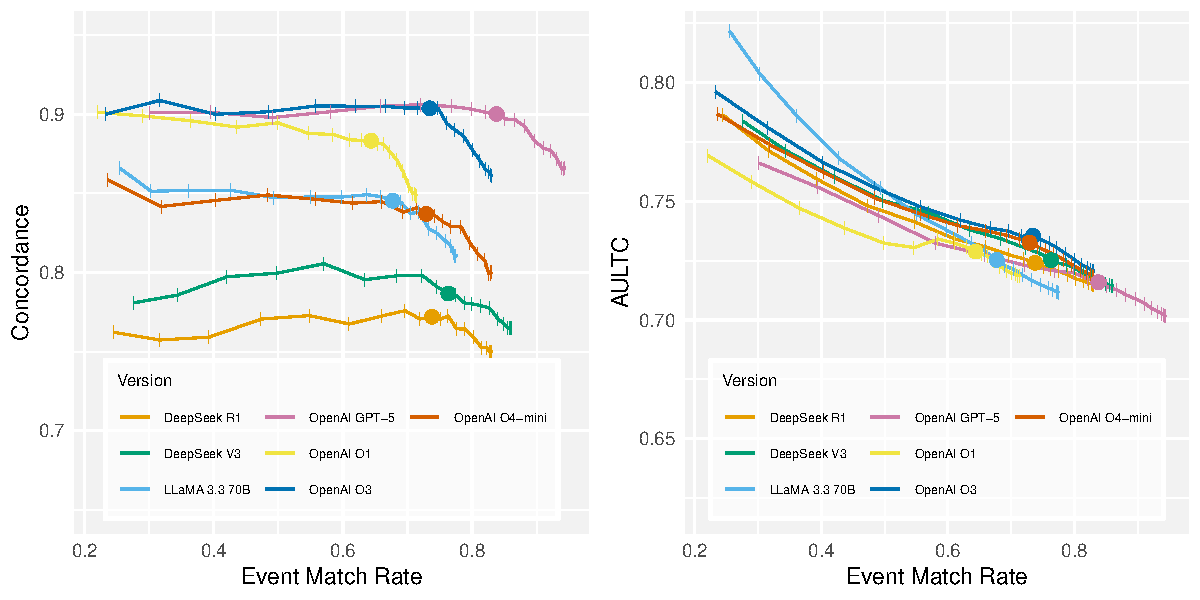
\includegraphics[width=\linewidth]{Chapters/chapter-05/images/Scientific_data/Plots_tables/event_match_vs_metrics_updated.pdf}

    
    
    

\end{ChFiveFloatBody}
\caption{Concordance and AULTC by event match rate for recursive matching heuristic. Solid circle ($\bullet$) represents threshold of 0.1, with ticks (|) indicating 0.01 increments of the threshold in [0.01, 0.50].
    }\ChFiveFloatLabel{ch05:fig:threshold_tradeoff_greedy}
\end{figure}





\paragraph{Inter-LLM comparison of temporal annotations}
Finally, we qualitatively compared temporal annotations produced by several LLMs on a representative case report to illustrate characteristic differences in event extraction and timestamping (Supplementary Material, Section~\ref{ch05:apd:inter-llm-comparison}, Figure~\ref{ch05:fig:tts_evaluation}).
While all models recovered the major clinical trajectory and preserved temporal polarity, they varied in
event granularity, paraphrasing, and long-range temporal normalization.
These differences complement the aggregate quantitative results and highlight the impact of model behavior on the structure of extracted timelines.
Common model-specific error patterns, such as granularity variation, duplicate events, and differences in temporal normalization, are summarized in the Supplementary Material, Section~\ref{ch05:apd:inter-llm-comparison}, Table~\ref{ch05:tab:error_taxonomy}.

\paragraph{Validation of Structured Fields}
\label{ch05:sec:structured-field-validation}

\ChFiveRebuttal{
We manually validated the structured fields on 88 confirmed case reports of \texttt{case\_study\_100} split. Across 264 demographic fields, 247 were correct (93.6\%): age accuracy was 95.5\% (84/88), sex accuracy was 97.7\% (86/88), and ethnicity accuracy was 87.5\% (77/88). Of 517 extracted diagnosis entries, 505 were supported by the source report, corresponding to 97.7\% precision. After revising the UMLS-linking procedure, 478/517 diagnosis mappings (92.46\%) were judged acceptable and 39/517 (7.54\%) incorrect.
}

\ChFiveRebuttal{
Demographic errors were concentrated in missing or malformed values; diagnosis errors primarily reflected family history, excluded differentials, or hypothetical complications assigned to the patient. UMLS errors most often involved an inappropriate semantic type or an overly generic concept.
}



% !TeX root = ../../../main.tex
\subsubsection{Limitations and Future Directions}
\label{ch05:sec:limitations-and-future-directions}

Our temporal annotation pipeline has several important limitations. 
\ChFiveRebuttal{
First, because published case reports preferentially describe unusual, severe, or diagnostically complex presentations, PMOA-TTS is not representative of routine clinical populations. Analyses of diagnosis frequencies should therefore be interpreted as descriptions of the corpus rather than estimates of disease prevalence.
}
\ChFiveRebuttal{
Demographic fields may contain unsupported inferences, missing-value errors, and category-mapping errors and should not be used as verified patient attributes without source-level review.
}
At the same time, we should still note that case reports offer rich, temporally structured narratives with explicit clinical rationale, making them a useful testbed for developing and stress-testing textual time series methods.
Our LLM-based framework is designed to be reusable and, in ongoing work, is being adapted to corpora such as MIMIC-IV discharge summaries for future dataset releases.

Second, we model events as minimally modified text spans aligned to the source narrative.
This design choice preserves interpretability and facilitates direct comparison with the underlying text but relies on embedding-based matching for evaluation and does not normalize event content to standard clinical ontologies such as UMLS. \ChFiveRebuttal{The free-text representation introduces lexical variation across reports. Synonym-aware retrieval and event-level mappings to controlled vocabularies may be added as downstream views of the data, but the source-faithful span should be retained so that normalization does not remove clinically important context or modifiers.}

Third, representing time with single relative points simplifies annotation and downstream use but cannot fully capture durations or complex temporal relations (e.g., overlapping intervals or recurrent events).

Fourth, our one-to-one recursive event matching strategy emphasizes temporal consistency at the expense of recall, especially when the same clinical concept is expressed multiple times or in conjunctive form.
Alternative matching formulations (e.g., many-to-many or cluster-based matching) could improve coverage but would require more elaborate evaluation protocols. 

These limitations point to several directions for future work, including ontology-aware event normalization, richer temporal representations (intervals and uncertainty), improved matching algorithms, and extension of the pipeline to diverse EHR-derived note types.


    
    

    
    



% !TeX root = ../../../main.tex
\begin{figure}[htbp]
\begin{ChFiveFloatBody}

\centering
    \begin{minipage}[t]{0.242\textwidth}
    \centering
    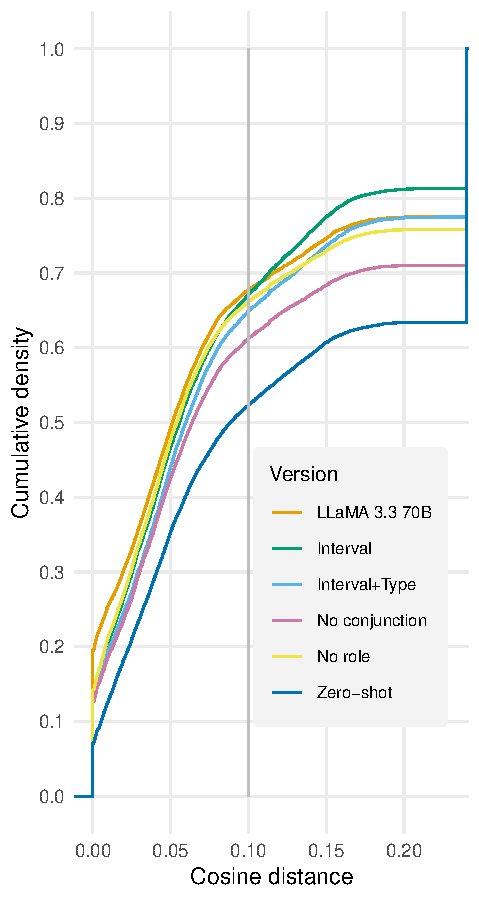
\includegraphics[page=1, width=\linewidth]{Chapters/chapter-05/images/Plots_tables/prompt_ablation_updated_figure.pdf}
    \end{minipage}
    \hfill
    \begin{minipage}[t]{0.242\textwidth}
    \centering
    \includegraphics[page=2, width=\linewidth]{Chapters/chapter-05/images/Plots_tables/prompt_ablation_updated_figure.pdf}
    \end{minipage}
    \hfill
    \begin{minipage}[t]{0.242\textwidth}
    \centering
    \includegraphics[page=3, width=\linewidth]{Chapters/chapter-05/images/Plots_tables/prompt_ablation_updated_figure.pdf}
    \end{minipage}
    \hfill
    \begin{minipage}[t]{0.242\textwidth}
    \centering
    \includegraphics[page=4, width=\linewidth]{Chapters/chapter-05/images/Plots_tables/prompt_ablation_updated_figure.pdf}
    \end{minipage}
    
    
    

\end{ChFiveFloatBody}
\caption{Comparison of \texttt{Llama 3.3 70B} prompt ablation and variant methods for extracting temporal clinical events from case reports. From left to right: (\textbf{A}) event match cumulative distribution function, (\textbf{B}) concordance box plots, (\textbf{C}) time discrepancy from manual annotation timestamps among matched events (overall), and (\textbf{D}) time discrepancy disaggregated by clinician annotator timestamp (time from presentation).}\ChFiveFloatLabel{ch05:fig:prompt_ablation}
\end{figure}















% % !TeX root = ../../../main.tex
\subsection{Usage Notes}
\label{ch05:sec:usage-notes}

Our full codebase, including preprocessing scripts, prompt templates, and evaluation pipelines,
is available at: \url{https://github.com/jcweiss2/pmoa_tts}.
Each subdirectory contains its own README.md with detailed instructions and information.
Here is the repository structure
\begin{itemize}
    \item \texttt{make\_tts}: Scripts and notebooks for constructing the PMOA-TTS dataset from case reports.
    \item \texttt{TTS\_evaluation}: Evaluation scripts assessing the quality of the extracted timelines.
\end{itemize}

\noindent Here are step-by-step directions on how to use the dataset

\begin{enumerate}

\item \textbf{Clone the repository:}

{\small
\begin{verbatim}
    git clone https://github.com/jcweiss2/pmoa_tts.git
    cd pmoa_tts
\end{verbatim}
}

\item \textbf{Set up the environment:}

\noindent Ensure you have Python 3.10 or higher installed. It's recommended to use a virtual environment.

{\small
\begin{verbatim}
    conda create -n pmoa_tts python=3.10
    conda activate pmoa_tts
    conda install pandas scikit-learn numpy tensorboard -c conda-forge
    conda install pytorch torchvision torchaudio -c pytorch
    pip install transformers
    pip install argparse
    conda install jupyter -c conda-forge
    pip install sentencepiece
\end{verbatim}
}

\item \textbf{Access the PMOA-TTS dataset.} The dataset is available on Hugging Face.
You can download it using the \texttt{datasets} library.

{\small
\begin{verbatim}
    from datasets import load_dataset
    dataset = load_dataset("snoroozi/pmoa-tts")
\end{verbatim}
}

\end{enumerate}

\ChFiveParagraph{Responsible reuse and cautions}

The release and use of PMOA–TTS raise important considerations.
Although LLMs achieve strong performance, they may still generate inaccurate or hallucinated outputs, and any downstream use of these annotations without further validation could introduce bias or error.
The extraction of structured diagnoses, demographics, and clinical events from public text—though non-identifiable—could also lead to misinterpretation or reinforce historical biases if not handled carefully.
Furthermore, while the dataset is intended for research, there is a risk of misapplication in high-stakes clinical settings without expert oversight.
Lastly, the stylistic and structural differences between case reports and real-world EHR notes may limit the generalizability of findings derived from PMOA–TTS.
These limitations underscore the importance of using the corpus responsibly, with clear reporting of model limitations and appropriate safeguards when applied in downstream tasks.



% % !TeX root = ../../../main.tex
\ChFiveStarSection{Code availability}\label{ch05:sec:data_availability}
In line with the philosophy of reproducible research, all codes used in this paper, including those for data preprocessing and technical validation, are accessible at \url{https://github.com/jcweiss2/pmoa_tts}. The usage instructions and parameter settings for all codes can be found at this link.


% % !TeX root = ../../../main.tex
\ChFiveStarSection{Funding}

This research was supported in part by the Division of Intramural Research (DIR) of the National Library of Medicine (NLM), National Institutes of Health.
This work utilized the computational resources of the NIH HPC Biowulf cluster.
S. N. was supported by Carnegie Mellon University TCS Presidential Fellowship, and Natural Sciences and Engineering Research Council of Canada (NSERC) PGS-D award.
S.N was also supported in part by an appointment to the National Library of Medicine Research Participation Program administered by the Oak Ridge Institute for Science and Education (ORISE) through an interagency agreement between the U.S. Department of Energy (DOE) and the National Library of Medicine, National Institutes of Health.
ORISE is managed by ORAU under DOE contract number DE-SC0014664.
All opinions expressed in this paper are the authors’ and do not necessarily reflect the policies and views of NIH, NLM, DOE, or ORAU/ORISE.



% % !TeX root = ../../../main.tex
\ChFiveStarSection{Author contributions}

These authors contributed equally: Shahriar Noroozizadeh (S.N.) and Sayantan Kumar (S.K.).
S.N. and S.K. implemented the pipeline, ran all experiments, curated the data, performed analyses and visualizations, and drafted/revised the manuscript.
Jeremy C. Weiss (J.C.W.) conceived the study, guided methodology, contributed to experiments, supervised the project, and secured funding.
George Chen (G.C.) contributed to technical discussions and manuscript review.
All authors approved the final manuscript.



\clearpage
\endgroup

% !TeX root = ../../main.tex
\chapter{Reconstructing Sepsis Trajectories from Clinical Text}\label{chap:ch06}
% !TeX root = ../../../main.tex
\ProposalPlaceholder{Temporary placeholder. The selected paper and its scientific abstract have not been migrated.}


% !TeX root = ../../main.tex
\chapter{Forecasting Clinical Risk from Textual Time Series}\label{chap:ch07}
% !TeX root = ../../../main.tex
\ProposalPlaceholder{Temporary placeholder. The selected paper and its scientific abstract have not been migrated.}


% !TeX root = ../../main.tex
\begingroup
\ChEightBegin
\emergencystretch=2em
\chapter{Text Knows What, Tables Know When: Clinical Timeline Reconstruction via Retrieval-Augmented Multimodal Alignment}\label{chap:ch08}
\noindent\emph{This chapter is based on:} \cite{kumar2026text}.\par\smallskip

% % !TeX root = ../../../main.tex
\begin{ChEightAbstract}
Clinical language models increasingly operate over electronic health records (EHRs), yet patient records are not stored as temporally grounded trajectories. Clinical notes describe symptoms, assessments, and disease progression, but often compress or narratively reorder events. Structured EHR rows provide timestamps for labs, medications, vitals, and procedures, but capture only part of the clinical story. We formulate clinical timeline reconstruction as retrieval-augmented temporal grounding: constructing a patient trajectory by using narrative text for event semantics and structured rows as partial temporal evidence. We introduce a scaffolded workflow that extracts central narrative events, builds an initial temporal scaffold, attaches non-central events, and calibrates timestamps using retrieved structured EHR rows. We evaluate on 40 discharge summaries, including 15 i2b2-derived and 25 MIMIC-IV summaries, each with manual gold-standard timelines and aligned structured EHR data. 
\ChEightRebuttal{Across models, multimodal calibration left event match rates largely unchanged and generally improved temporal performance: mean paired case-level multimodal--unimodal differences were positive in 7 of 12 model-metric comparisons across concordance and AULTC, with none negative. However, uncertainty was substantial given the 40-case sample; paired case-level bootstrap intervals excluded zero only for the DeepSeek V3.2 AULTC improvement.}
A gap analysis shows that 35.1\% of text-derived events have no structured counterpart. These findings support treating structured EHR data as partial temporal evidence for narrative-derived patient trajectories.
\end{ChEightAbstract}

\ChEightKeywords{Clinical timeline reconstruction; electronic health records; clinical narratives; retrieval-augmented generation; multimodal alignment; large language models}


% required, do-not-remove
% \ChEightContributionNote{$^{\ast}$ These authors contributed equally to this work.}

%%%%%%%%%%%%%%%%%%%%%%%%%%%%%%%%%%%%%%%%%%%%%%%%%%


%%%%%%%%%%%%%%%%%%%%%%%%%%%%%%%%%%%%%%%%%%%%%%%%%%


% !TeX root = ../../../main.tex
\subsection{Introduction}


Time is central to clinical reasoning in critical care.
% ICU p
Patients often follow rapidly evolving trajectories, requiring symptoms, physiologic measurements, treatments, and outcomes to be interpreted relative to admission, deterioration, intervention, and recovery. 
% Sepsis exemplifies this challenge. 
Sepsis trajectories exemplify this challenge.
Although Sepsis-3 remains important for trial eligibility and computational phenotyping \cite{kyriazopoulou2021procalcitonin,ch08:seymour2019derivation}, 
% sepsis is better understood as a heterogeneous clinical trajectory than as a single, uniform state. 
sepsis is better understood as a set of heterogeneous clinical trajectories with a shared dysregulatory response rather than as a single, uniform course. 
Similar temporal challenges extend across critical illness: risk forecasts depend on when evidence becomes available; treatment-response analyses require distinguishing pre- and post-intervention measurements; and retrospective cohort definitions may change when the timing of symptom onset, diagnostic testing, or treatment initiation is misaligned.
This increasing focus on temporal structure is evident in early-warning systems \cite{henry2022factors}, studies showing that predictive utility varies with timing \cite{kamran2024evaluation}, and research on the temporal characteristics of sepsis subtypes and progression \cite{ch08:noroozizadeh2023temporal}.


The growing emphasis on time in critical care reveals an important methodological gap: electronic health records (EHRs) are not organized as temporally grounded patient trajectories. Critical-care repositories such as MIMIC-III/IV \cite{ch08:johnson2016mimic,ch08:johnson2023mimic} make this challenge explicit by combining structured time-series measurements with narrative clinical documentation. These modalities provide complementary but asymmetric evidence for timeline construction (Figure~\ref{ch08:fig:motivation_multimodal_alignment}). Structured rows offer relatively precise temporal information from laboratory results, medications, procedures, vital signs, diagnoses, and administrative events. Clinical narratives, by contrast, provide richer accounts of the patient course, including symptoms, clinician assessments, patient-reported histories, functional status, disease progression, and contextual modifiers. For example, a note describing ``increasing lethargy and peripheral mottling'' may precede an increase in Sequential Organ Failure Assessment (SOFA) scores. Similarly, documented oliguria despite stable creatinine may indicate clinically meaningful states that structured measurements do not fully capture. 

Recent studies point to both the promise and the difficulty of this problem. Multimodal annotation of discharge summaries aligned with structured EHR data demonstrated that access to both modalities can improve the precision of inpatient event timelines, highlighting the value of structured rows as temporal evidence when aligned with the narrative record \cite{ch08:frattallone2024using}. At the same time, text-only timeline reconstruction remains challenging in realistic EHR-style notes, where dense event structure, abbreviations, and semi-structured formatting make both event recovery and time assignment difficult \cite{noroozizadeh2026reconstructing,ch08:noroozizadeh2026forecasting}. Together, these findings motivate more explicit alignment between text-based and tabular approaches, with the goal of improving temporal precision while preserving the richer event content available in narrative text.\cite{ch08:moldwin2021empirical,seinen2025using}

In this work, we investigate whether aligning retrieved structured EHR evidence with text-derived event timelines can improve the temporal precision of reconstructed patient trajectories. Our retrieval-augmented multimodal approach integrates structured rows directly into timeline reconstruction rather than treating textual and tabular data as separate views. The multistep pipeline first identifies temporally informative central events and uses them to create an initial scaffold of the patient trajectory. It then positions additional events relative to this scaffold and refines the resulting timeline using retrieved structured evidence. This decomposition reflects a clinically natural distinction between events that form the backbone of an encounter and those whose timing is best interpreted relative to that backbone. Using this framework, we assess whether and where multimodal alignment improves on text-only timeline reconstruction. Specifically, we examine the effects of introducing structured evidence at different stages of the reconstruction workflow, determine whether improvements are concentrated in temporal metrics rather than event recovery, and analyze which prognostically relevant information appears in text but is missing or delayed in tabular data.

%%%%%%%%%%%%%%%%%%%%%%%%%%%%%%%%%%%%%%%%%%%%%%%%%%

% !TeX root = ../../../main.tex
\begin{figure}[htbp]
\begin{ChEightFloatBody}

    \centering
    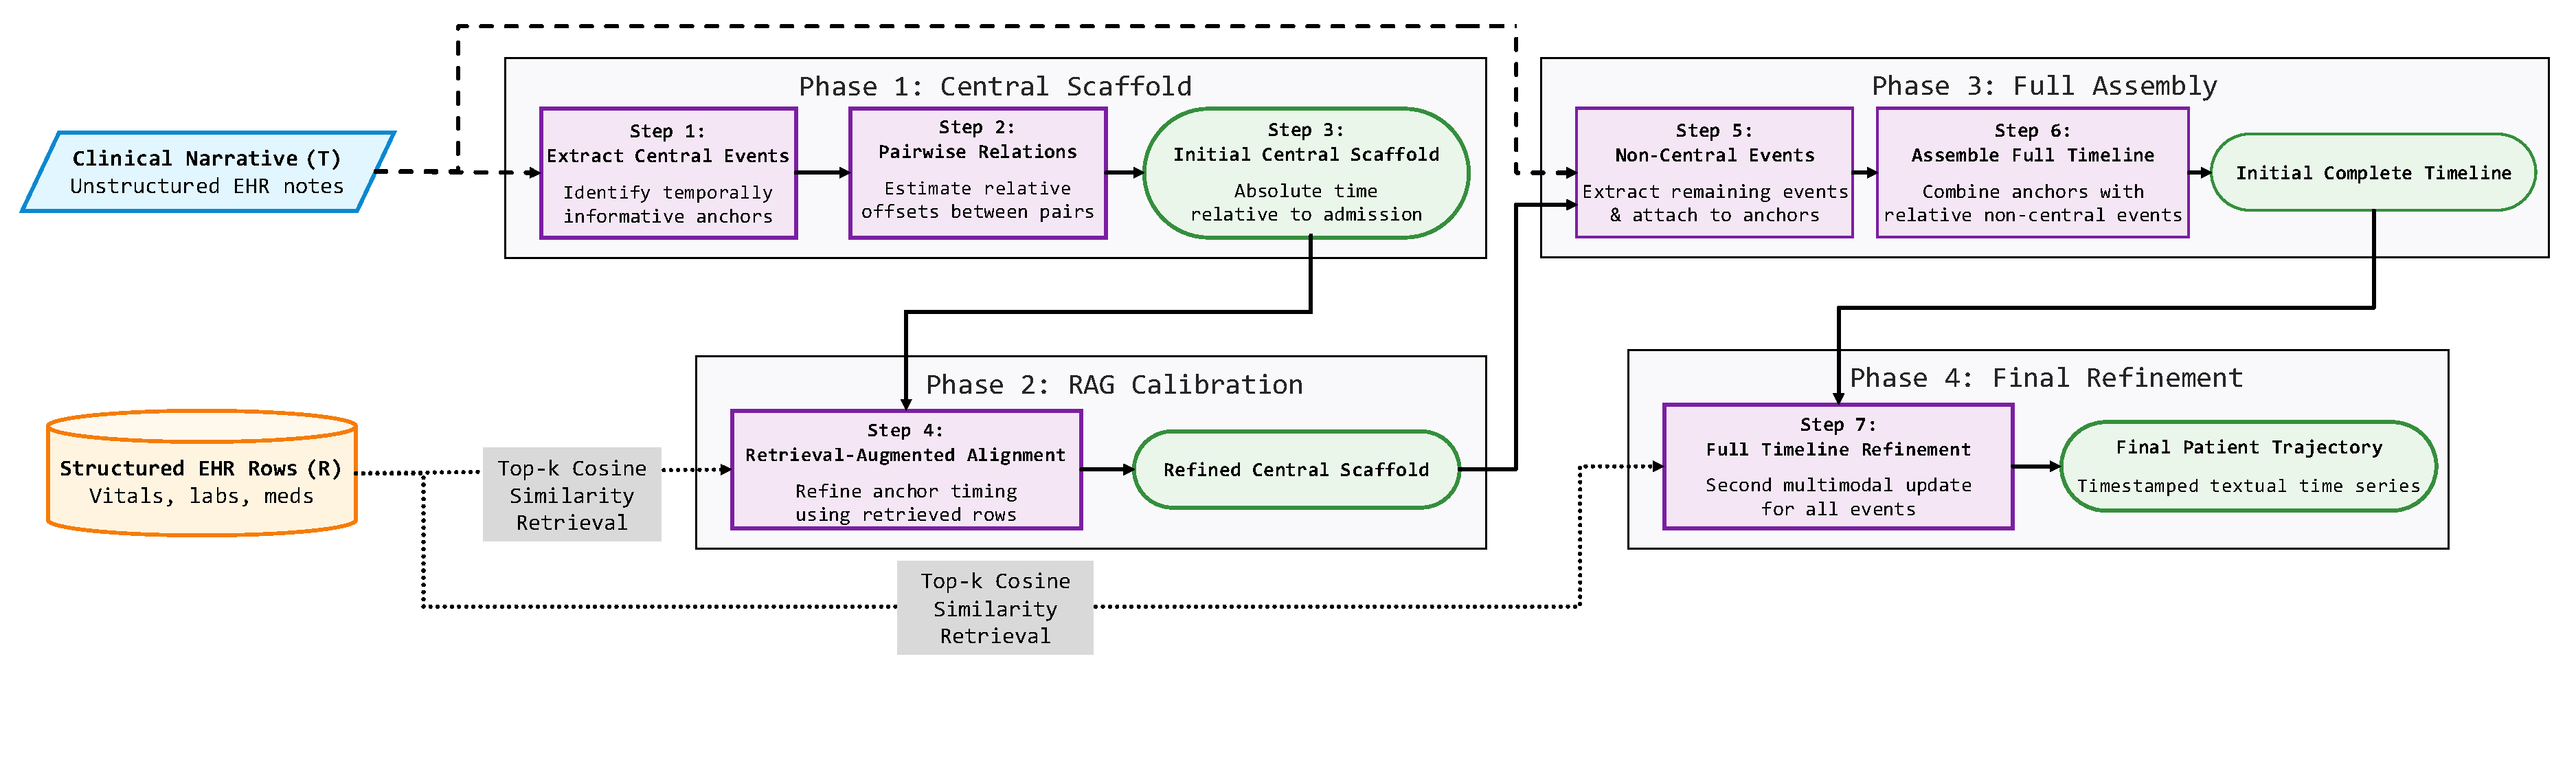
\includegraphics[width=\textwidth]{Chapters/chapter-08/images/plots/TTA-Overview-Figure-Model-Updated.pdf}
    
    
    
    

\end{ChEightFloatBody}
\caption{
    Overview of the scaffolded retrieval-augmented timeline reconstruction workflow. The method first extracts central events from the clinical narrative, estimates pairwise temporal relations, and builds an initial central-event scaffold. Retrieved structured EHR rows are then used to calibrate this scaffold. Non-central events are extracted and attached relative to central events, after which a final retrieval-augmented refinement step calibrates the complete timeline.
    % \textcolor{blue}{Shahriar-update figure to remove symbols if relevant}
    }\ChEightFloatLabel{ch08:fig:pipeline}
\end{figure}

%%%%%%%%%%%%%%%%%%%%%%%%%%%%%%%%%%%%%%%%%%%%%%%%%%

% \vspace{-5pt}
\textbf{Contributions.} In summary, the paper makes the following contributions. \textbf{(i) Temporal grounding formulation:} We formulate clinical timeline reconstruction as retrieval-augmented temporal grounding of narrative-derived patient trajectories using structured EHR evidence. \textbf{(ii) Multimodal scaffolded reconstruction workflow:} We introduce a workflow that uses anchor events as a temporal backbone and retrieved structured rows as partial evidence for timestamp calibration. \textbf{ (iii) Multimodal timeline evaluation:} We evaluate multimodal calibration on 40 discharge summaries with aligned structured EHR rows and manual gold-standard timelines, testing whether structured evidence improves temporal localization more than event recovery. \textbf{(iv) Information missing from tabular data:} We provide an empirical analysis of clinically relevant events that are absent, delayed, or semantically compressed in structured tabular data, motivating why unstructured text is necessary for constructing clinically meaningful patient trajectories.
% \textcolor{blue}{Shahriar - if you can manage space, feel free to add uncertainty analyses and update relevant sections}
%\textcolor{blue}{\textbf{(v) When multimodal alignment helps most:} We characterize performance across event types and timestamp-certainty settings, showing that structured data is especially useful as a temporal calibrator when event timing cannot be directly inferred from text.}

%%%%%%%%%%%%%%%%%%%%%%%%%%%%%%%%%%%%%%%%%%%%%%%%%%
%%%%%%%%%%%%%%%%%%%%%%%%%%%%%%%%%%%%%%%%%%%%%%%%%%


% !TeX root = ../../../main.tex
\subsection{Related Work}
\label{ch08:sec:related_work}


\textbf{Clinical temporal information extraction.}
Clinical timeline reconstruction builds on a long tradition of temporal reasoning and temporal information extraction in medicine \cite{ch08:kohane1987temporal,zhou2007temporal}.
Early annotation schemes and shared tasks, including i2b2 and THYME, focused on identifying clinical events, time expressions, and temporal relations such as before, after, overlap, and containment \cite{ch08:uzuner20112010,sun2013evaluating,sun2013annotating,ch08:styler2014temporal}.
Systems such as MedTime and cTAKES-temporal operationalized these ideas for clinical notes by extracting time expressions and temporal relations \cite{lin2013medtime,savova2010mayo,lin2016multilayered}.
Pre-LLM work also studied patient timelines and longitudinal record summarization, including timeline generation from clinical notes and HARVEST for summarizing longitudinal patient records \cite{nikfarjam2013towards,hirsch2015harvest}.
These studies established the importance of temporal structure in clinical narratives, but primarily focused on temporal annotation, relation extraction, or summarization rather than grounding narrative-derived absolute timelines in structured EHR evidence.


\noindent
\textbf{LLM-based clinical timeline reconstruction.}
Recent work has moved from relation-centered temporal extraction toward absolute event timelines.
Leeuwenberg and Moens studied absolute event timeline extraction from English clinical reports, while Frattallone-Llado et al. showed that aligning discharge summaries with structured EHR data can improve inpatient event timeline precision \cite{leeuwenberg2020towards,ch08:frattallone2024using}.
Textual time-series work has further shown that clinical narratives can be converted into event--time tuples for temporal forecasting, but these approaches are primarily text-only and do not use structured EHR rows as calibration evidence during reconstruction \cite{ch08:wang2025large,noroozizadeh2026reconstructing,ch08:noroozizadeh2026forecasting,ch08:kumar2026temporally}.
Recent shared tasks such as ChemoTimelines have renewed interest in patient-level clinical timeline extraction using prompting, fine-tuning, and dictionary-enhanced LLM systems \cite{yao2025chemotimelines,zhang2025uwbionlp}.
Our work differs from these efforts by treating timeline reconstruction as multimodal temporal grounding: narrative text supplies event semantics, while structured EHR rows are retrieved as partial temporal evidence for timestamp calibration.


\noindent
\textbf{Asymmetric evidence in structured and narrative EHR data.}
Clinical machine learning studies have shown that structured and unstructured EHR data encode complementary information for phenotyping, prediction, and patient representation \cite{ch08:moldwin2021empirical,liu2022multimodal,seinen2025using}.
Structured data provide dense timestamped measurements, but often omit symptoms, functional status, patient-reported histories, and clinical reasoning.
Narrative notes preserve this context, but are often retrospective and not organized as chronological trajectories.
This asymmetry makes clinical timeline reconstruction different from standard multimodal fusion: the goal is not to merge two complete views of the same event sequence, but to use structured rows as partial temporal evidence for a narrative-derived patient trajectory.
Our retrieval-augmented scaffolded workflow is designed for this setting, selecting candidate structured rows for each text-derived event and updating timestamps only when the retrieved evidence is clinically relevant.



% !TeX root = ../../../main.tex
\subsection{Methods}
\label{ch08:sec:methods}
\ChEightHeadingOnly


\subsubsection{Clinical timeline task and dataset}
\label{ch08:sec:data}


Given a clinical narrative $T$ and associated structured EHR rows $R$, the goal is to reconstruct a textual time series $\hat{S}=\{(e_i,\hat{t}_i)\}_{i=1}^{N}$, where each $e_i$ is a standalone clinical event and each $\hat{t}_i \in \mathbb{R}$ is its predicted timestamp in hours relative to a case-specific reference time.
When hospital admission is explicitly described, we use admission as $t=0$; otherwise, we use the earliest documented clinical encounter or presentation in the narrative.
Events before the reference time receive negative timestamps, and events after it receive positive timestamps.

A clinical event is any patient-specific health-related mention that is semantically interpretable on its own and temporally locatable, including symptoms and signs, diagnoses, tests, procedures, treatments, medication administrations, major clinical states, outcomes, pertinent negatives, and termination or discontinuation events.
Our event representation follows prior textual time-series work \cite{ch08:wang2025large,noroozizadeh2026reconstructing,ch08:noroozizadeh2025pmoa,ch08:kumar2026temporally}, but differs from short-span, concept-centric schemes such as i2b2 \cite{ch08:uzuner20112010,sun2013evaluating}.
We represent events as standalone clinical findings: spans may include context needed for clinical specificity, conjunctive mentions are split when doing so improves clarity, and modifiers such as negation, uncertainty, severity, laterality, and intent are preserved when they affect event interpretation or temporal placement.

Our evaluation uses \textbf{40 discharge summaries} with manual gold-standard timelines and aligned structured EHR rows: \textbf{15 i2b2-derived discharge summaries} and \textbf{25 MIMIC-IV discharge summaries}.
All cases have structured EHR rows aligned to the same hospital encounter.
MIMIC-style critical-care records are well suited for this setting because they pair narrative clinical documentation with timestamped structured data, including laboratory values, medication administrations, vital signs, procedures, diagnoses, and administrative events \cite{ch08:johnson2016mimic,ch08:johnson2023mimic}.
For each case, the narrative note provides the source text for event reconstruction, while the structured record provides external temporal evidence.
We convert structured-row timestamps to hours relative to the same case-specific reference time used for the narrative timeline.
Each structured row $r_m \in R$ is represented as $r_m=(\nu_m,x_m,s_m)$, where $\nu_m$ is the row name or clinical feature, $x_m$ is the observed value when available, and $s_m$ is the timestamp in hours relative to the reference time.

\ChEightRebuttal{The 15 i2b2-derived cases were randomly sampled from eligible cases; the 25 MIMIC-IV cases were sampled at the patient level, using the first discharge summary for five randomly sampled patients and one randomly selected summary for 20 others, without enrichment for diagnosis, temporal richness, or encounter complexity. Three medical experts annotated disjoint subsets; every case was annotated once from the note and aligned structured record, so no adjudication or inter-annotator agreement was available (\hyperref[ch08:supp:eval-cohort]{Supplementary Material \S\ref*{ch08:supp:eval-cohort}}).}

We treat structured rows as temporal evidence rather than gold-standard timeline events.
Structured EHR tables contain dense repeated measurements, medication records, and machine-generated entries, many of which are not standalone narrative events.
Conversely, clinically meaningful narrative events, such as symptoms, functional status, patient-reported histories, and clinical reasoning, may not have direct structured counterparts.
Our method therefore uses structured rows to calibrate text-derived event times when clinically relevant, rather than forcing all structured rows into the reconstructed timeline.




\subsubsection{Scaffolded retrieval-augmented multimodal timeline reconstruction}
\label{ch08:sec:pipeline}


Our workflow is designed around three principles.
First, it anchors before expanding: the model identifies temporally informative anchor events before reconstructing the full event set.
Second, it retrieves candidate structured evidence rather than forcing every narrative event to align to a structured row.
Third, \ChEightRebuttal{it uses preserve-by-default calibration}: event times are updated only when retrieved structured evidence is clinically relevant and temporally plausible.
The workflow proceeds in seven clinically interpretable steps (Figure \ref{ch08:fig:pipeline}).\footnote{Step-specific prompts and the full reproducibility pipeline are available in our GitHub repository:\\\url{https://github.com/SayantanKumar/multimodal_textual_tabular_alignment}}

\begin{enumerate}
    \item \textbf{Step 1: Extract anchor events.} The model first identifies temporally informative anchor events, also referred to as central events, that define the encounter backbone or serve as temporal referents for other events.
Examples include admission, symptom onset, treatment initiation, clinical deterioration, procedures, transfers, and discharge. 

    \item \textbf{Step 2: Estimate timing among anchors.} The model estimates pairwise time differences (in hours) between selected anchor events.

    \item \textbf{Step 3: Build an initial anchor timeline.} The pairwise relations between anchor events are resolved into a provisional timeline backbone in hours relative to the case reference time.
When estimates conflict, the model uses higher-confidence relations and the source narrative to construct the initial scaffold.

    \item \textbf{Step 4: Calibrate anchors using structured evidence.} For each anchor event, retrieved structured EHR rows are provided to the calibration model together with the narrative and provisional scaffold.
The model updates an anchor time only when the structured row clinically supports the change; otherwise, the text-derived estimate is retained.

    \item \textbf{Step 5: Extract non-anchor supporting events relative to anchors.} After anchor calibration, the model extracts remaining non-anchor events and attaches each event to a referent anchor with a relative time offset and confidence score.
These events include symptoms, exam findings, pertinent negatives, severity descriptors, functional status, medication details, and contextual clinical information.
    
    \item \textbf{Step 6: Assemble the full timeline.} The calibrated anchor times and relative supporting-event offsets are combined into an initial complete timeline, converting all events into absolute times in hours relative to the case reference time.
    
    \item \textbf{Step 7: Refine the complete timeline using structured evidence.} Structured rows are retrieved again for all reconstructed events, not only anchors.
The model performs a final conservative calibration pass, updating timestamps when retrieved rows provide clinically consistent temporal evidence and preserving text-derived times otherwise.
The output is a temporally grounded textual time series containing clinically meaningful narrative events with calibrated timestamps when structured evidence is relevant.
\end{enumerate}


\ChEightParagraph{Retrieval and calibration module.}
The same retrieval module is used in Step 4 and Step 7. Structured rows are represented by concatenating the row event name and value; timestamps are excluded from the embedding text and passed separately to the calibration model.
Rows with the same event name and value are merged, with timestamps represented in hours relative to the case reference time.
We embed event strings and structured-row representations using MedTE (\texttt{mohammadkhodadad/MedTE-cl15-step-8000}), mean-pool and L2-normalize the embeddings, and rank rows by cosine similarity.
For each event, we retrieve the top $k=5$ structured rows with no fixed similarity threshold.
The calibration model receives each row as \texttt{name | value | time | similarity}. \ChEightRebuttal{Calibration follows a preserve-by-default rule: cosine similarity ranks candidates, irrelevant rows are disregarded, the initial time is retained when no relevant evidence justifies a change, and narrative context resolves repeated timestamps or conflicting rows. The complete decision rule appears in \hyperref[ch08:supp:calibration-rule]{Supplementary Material \S\ref*{ch08:supp:calibration-rule}}.}
We also evaluated $k=3$, $k=5$, and $k=10$, finding negligible performance differences but increased runtime for larger $k$.

This design treats retrieval as evidence selection rather than forced temporal alignment.
Methods such as dynamic time warping assume that two sequences share an approximately comparable event universe and can be aligned through a monotone path.
Clinical narratives and structured EHR rows often violate this assumption: many narrative events have no structured counterpart, while structured tables contain dense repeated measurements, medication records, and charted observations that are not standalone narrative events.
Our workflow therefore allows structured evidence to calibrate event times when appropriate without requiring every narrative event to have a tabular match.


\subsubsection{Experimental setup}
\label{ch08:sec:experimental_setup}


\textbf{Baselines and ablations.} We compare the default scaffolded multimodal workflow against text-only, single-step, stage-specific, and forced-alignment baselines. \textbf{Text-only reconstruction} uses the same scaffolded workflow but removes both structured-EHR calibration steps, testing whether retrieved structured evidence improves temporal localization beyond narrative-only reconstruction. \textbf{Single-step multimodal reconstruction} directly generates a complete timeline from the narrative and retrieved structured rows without constructing an anchor-event scaffold, testing whether the staged anchor/non-anchor decomposition is useful beyond simply adding retrieved evidence to the prompt. To isolate where structured evidence contributes, we compare two stage-specific ablations: \textbf{anchor-only calibration}, which calibrates the anchor scaffold but omits final full-timeline calibration, and \textbf{final-only calibration}, which reconstructs the full timeline from text before applying structured-EHR calibration. The default workflow applies both anchor-stage and final-stage calibration. Finally, \textbf{dynamic time warping (DTW)} serves as a forced temporal-alignment baseline that attempts to align text-derived events with structured rows through sequence alignment rather than retrieval-based evidence selection followed by clinical calibration.


\noindent\textbf{Evaluation metrics.} We evaluate predicted timelines along two complementary dimensions: \emph{event recovery} and \emph{temporal localization}, adapted from prior textual time-series work \cite{ch08:wang2025large,noroozizadeh2026reconstructing}. Because predicted and reference timelines may differ in length and event wording, we first align predicted events to manually annotated reference events using a recursive best-match procedure. This produces a one-to-one alignment between predicted and reference events while accommodating unequal timeline lengths. \textbf{Event match rate} is the proportion of reference clinical events successfully aligned to a predicted event. Temporal metrics are computed on the matched subset. \textbf{Temporal concordance} (c-index) measures whether the predicted timeline preserves the relative ordering of events in the manual reference. \textbf{Area Under the Log-Time Cumulative Distribution Function (AULTC)} summarizes absolute timestamp discrepancy on a log-transformed time scale, with higher values indicating smaller timestamp errors across clinically meaningful ranges. Because concordance and AULTC are computed only over matched events, they should be interpreted jointly with event match rate. 
We estimate uncertainty using case-level bootstrap confidence intervals.
Each bootstrap sample resamples discharge summaries with replacement and recomputes event matching and timeline metrics, preserving within-case dependence among events.
We report 95\% confidence intervals for the reconstruction metrics using 200 bootstrap resamples.
\ChEightRebuttal{For direct multimodal--unimodal comparisons, we additionally used 10,000 paired case-level resamples and report
confidence intervals for the mean within-case differences in \hyperref[ch08:supp:paired-bootstrap]{Supplementary Material \S\ref*{ch08:supp:paired-bootstrap}}, \hyperref[ch08:tab:supp-paired-bootstrap]{Table~\ref*{ch08:tab:supp-paired-bootstrap}}.} 
\ChEightRebuttal{All implementation and reproducibility details are presented in \hyperref[ch08:supp:implementation]{Supplementary Material \S\ref*{ch08:supp:implementation}}.}









% !TeX root = ../../../main.tex
\subsection{Results}
\label{ch08:sec:results}
\ChEightHeadingOnly


\subsubsection{\ChEightRebuttal{Structured EHR evidence calibrates event timing while preserving event recovery}}
\label{ch08:sec:main_results}

Table~\ref{ch08:tab:main_results_threshold_01} summarizes timeline reconstruction performance for text-only reconstruction and multimodal reconstruction with retrieved structured EHR evidence.
Across models, multimodal calibration has little effect on event match rate, indicating that structured rows do not primarily expand the set of events recovered from narrative text.
Instead, structured evidence primarily affects temporal localization, with effects that vary by model and metric.
These results support the role of structured rows as temporal evidence for text-derived events, rather than as a substitute event source.

\ChEightRebuttal{
Mean paired case-level temporal differences generally favored multimodal calibration: 4 of 6 models showed higher concordance and 3 of 6 showed higher AULTC, while no model showed lower performance on either temporal metric. However, uncertainty was substantial: no paired confidence interval for the multimodal--unimodal concordance difference excluded zero, and only DeepSeek V3.2 showed an AULTC interval entirely above zero ((\hyperref[ch08:supp:paired-bootstrap]{Supplementary Material \S\ref*{ch08:supp:paired-bootstrap}}, \hyperref[ch08:tab:supp-paired-bootstrap]{Table~\ref*{ch08:tab:supp-paired-bootstrap}})). Performance was generally higher on the i2b2-derived subset, but modality effects were source-dependent ((\hyperref[ch08:supp:dataset-stratified]{Supplementary Material \S\ref*{ch08:supp:dataset-stratified}}, Tables~\hyperref[ch08:tab:supp-i2b2]{\ref*{ch08:tab:supp-i2b2}}--\hyperref[ch08:tab:supp-mimiciv]{\ref*{ch08:tab:supp-mimiciv}})).}

Because event match rate depends on the semantic matching threshold used to align predicted and reference events, we also vary the event-matching threshold and examine the relationship between event recovery and temporal quality.
Figure~\ref{ch08:fig:threshold_sweeps_main} shows AULTC and concordance as functions of event match rate across thresholds.
Across operating points, multimodal reconstruction generally occupies a similar event-recovery range as text-only reconstruction while changing temporal performance, especially AULTC, for several models.
This supports the same broad conclusion as Table~\ref{ch08:tab:main_results_threshold_01}: retrieved structured rows primarily affect temporal calibration rather than event discovery.



% !TeX root = ../../../main.tex
\begin{table}[htbp]
\caption{Performance on 40 discharge summaries at event-matching threshold $0.1$ for unimodal and multimodal timeline reconstruction. Values are point estimates with bootstrap 95\% confidence intervals in brackets. \textbf{Bold} indicates the best point estimate within each metric--modality column.}\ChEightFloatLabel{ch08:tab:main_results_threshold_01}
\ChEightTableBodyStart
\begin{ChEightFloatBody}

{\footnotesize
\setlength{\tabcolsep}{3pt}
\renewcommand{\arraystretch}{1.12}

\begin{adjustbox}{max width=\textwidth}
\begin{tabular}{lcccccc}
\hline
\multirow{2}{*}{\textbf{Model}} 
& \multicolumn{2}{c}{\textbf{Event match rate}} 
& \multicolumn{2}{c}{\textbf{Concordance}} 
& \multicolumn{2}{c}{\textbf{AULTC}} \\
\cline{2-7}
& \textbf{Unimodal} & \textbf{Multimodal} 
& \textbf{Unimodal} & \textbf{Multimodal} 
& \textbf{Unimodal} & \textbf{Multimodal} \\
\hline
DeepSeek R1
& 0.39 [0.32, 0.47]
& 0.39 [0.32, 0.47]
& 0.75 [0.69, 0.79]
& 0.75 [0.70, 0.80]
& \textbf{0.80 [0.76, 0.82]} 
& \textbf{0.79 [0.77, 0.82]}\\

KimiK2-Instruct
& 0.26 [0.21, 0.29]
& 0.25 [0.22, 0.30]
& 0.73 [0.69, 0.76]
& 0.74 [0.68, 0.81]
& 0.68 [0.61, 0.73]
& 0.68 [0.62, 0.73] \\

GPT-OSS-120B
& 0.32 [0.27, 0.37]
& 0.32 [0.28, 0.37]
& 0.74 [0.70, 0.77]
& 0.75 [0.71, 0.80]
& 0.76 [0.72, 0.80] 
& 0.77 [0.74, 0.81]\\

DeepSeek V3.2
& \textbf{0.49 [0.43, 0.56]}
& \textbf{0.49 [0.43, 0.56]}
& 0.74 [0.70, 0.80]
& 0.77 [0.73, 0.81]
& 0.71 [0.64, 0.78] 
& 0.77 [0.73, 0.81]\\

GLM5
& 0.33 [0.27, 0.39]
& 0.33 [0.27, 0.40]
& \textbf{0.80 [0.78, 0.83]}
& \textbf{0.82 [0.75, 0.84]}
& 0.78 [0.73, 0.82] 
& 0.78 [0.73, 0.82]\\

Qwen3.5-397B-A17B
& 0.38 [0.28, 0.47]
& 0.40 [0.29, 0.51]
& 0.78 [0.72, 0.81]
& 0.79 [0.78, 0.82]
& 0.74 [0.68, 0.77] 
& 0.77 [0.74, 0.78]\\

\hline
\end{tabular}
\end{adjustbox}


}


\end{ChEightFloatBody}
\end{table}



% !TeX root = ../../../main.tex
\begin{figure}[htbp]
\begin{ChEightFloatBody}

    \centering
    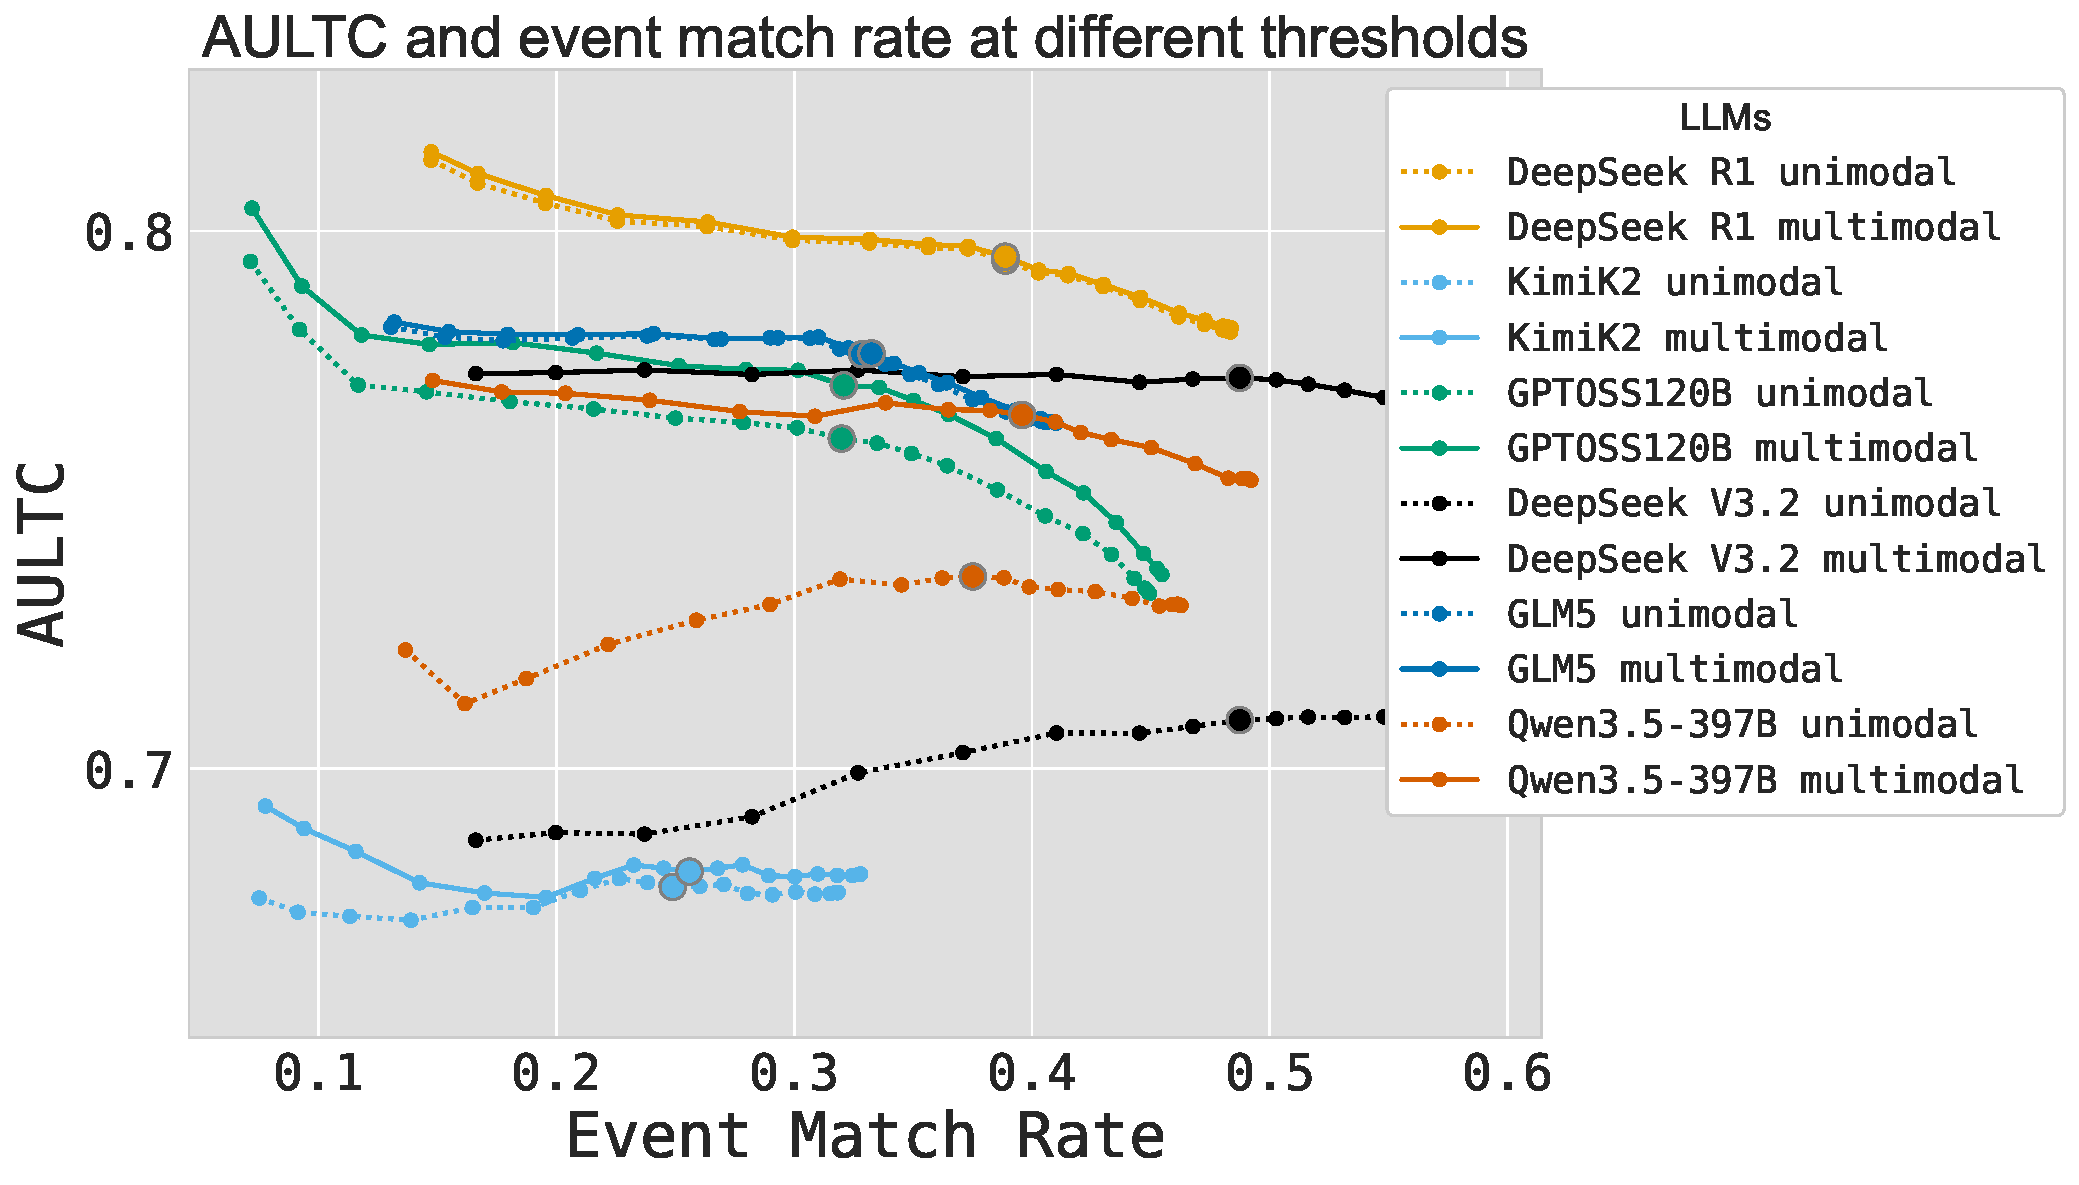
\includegraphics[width=0.479\textwidth]{Chapters/chapter-08/images/plots/aultc_vs_emr_n40_v2.pdf}
    \hfill
    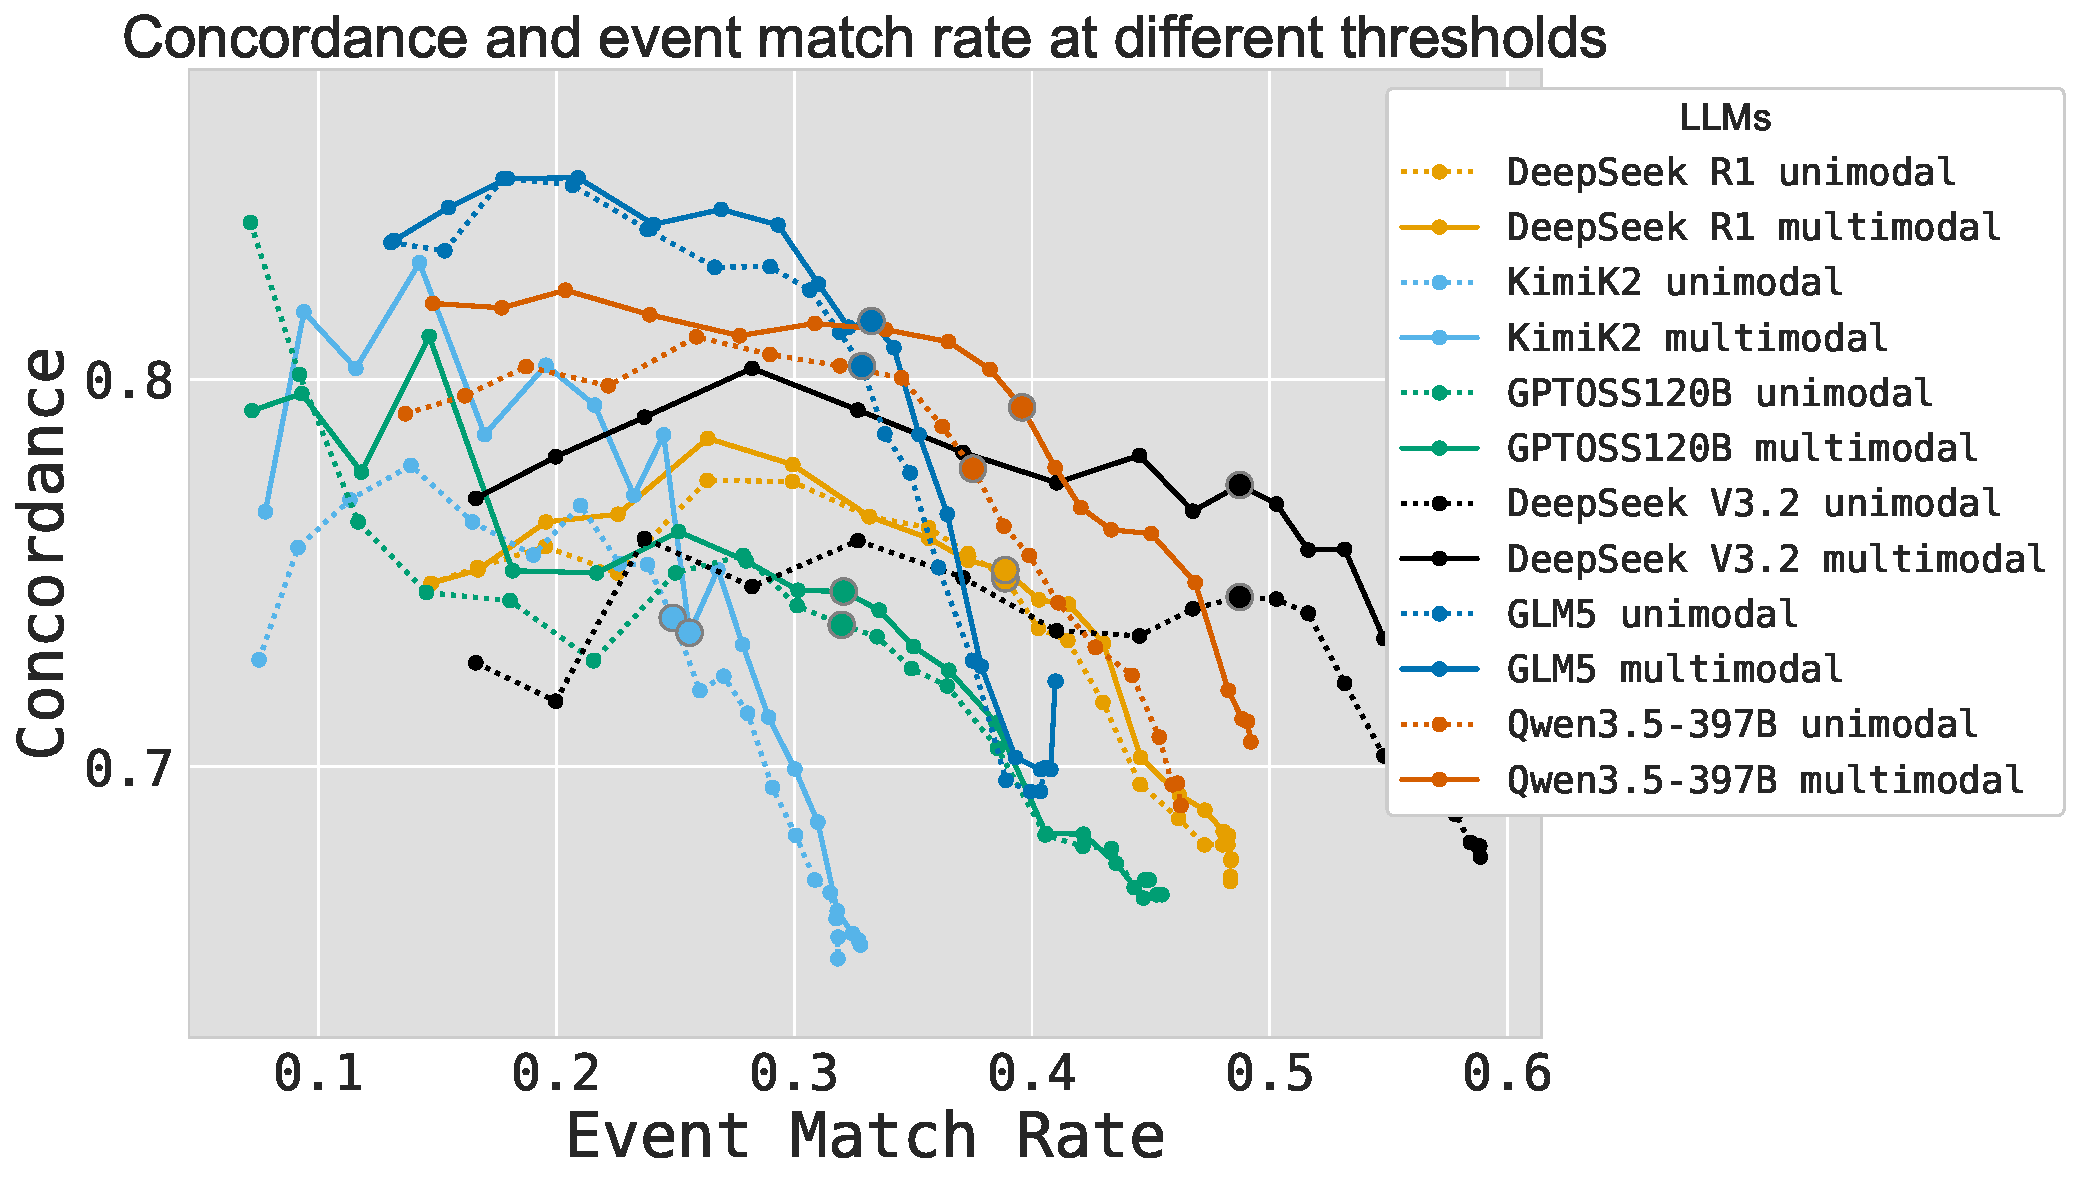
\includegraphics[width=0.479\textwidth]{Chapters/chapter-08/images/plots/cidx_vs_emr_n40_v2.pdf}

    
    \begin{minipage}[t]{0.485\textwidth}
        \centering
    \end{minipage}
    \hfill
    \begin{minipage}[t]{0.485\textwidth}
        \centering
    \end{minipage}

    
    
    
    

\end{ChEightFloatBody}
\caption{Temporal performance versus event match rate across event-matching thresholds for unimodal and multimodal variants of each model on the 40-summary evaluation set. (\textbf{Left}) AULTC versus event match rate. (\textbf{Right}) Temporal concordance versus event match rate.}\ChEightFloatLabel{ch08:fig:threshold_sweeps_main}
\end{figure}




\noindent\textbf{Scaffold ablations.}
Table~\ref{ch08:tab:ablation_and_DTW}A evaluates whether the staged scaffolded workflow is necessary, or whether similar performance can be obtained by generating a complete timeline in one step with retrieved structured rows.
The single-step formulation performs worse than the full scaffolded variant, suggesting that clinical timeline reconstruction benefits from first identifying temporally informative anchor events before reconstructing the full event set.
The stage at which structured evidence is introduced also matters.
Final-stage calibration yields the highest event match rate, but the strongest temporal metrics are obtained when structured evidence is used both to calibrate the anchor scaffold and to refine the final assembled timeline.
This supports the design choice of using structured rows first to stabilize the temporal backbone of the encounter and then to recalibrate the expanded trajectory.


% !TeX root = ../../../main.tex
\begin{table}[htbp]
\caption{\ChEightRebuttal{\textbf{(A)} DeepSeek V3.2 scaffold and calibration-stage ablations with bootstrap 95\% confidence intervals. \textbf{(B)} Retrieval calibration compared with sentence-embedding and lexical Dynamic Time Warping (DTW) alignments.}}\ChEightFloatLabel{ch08:tab:ablation_and_DTW}
\ChEightTableBodyStart
\begin{ChEightFloatBody}
 
\setlength{\tabcolsep}{3pt} \renewcommand{\arraystretch}{1.08} 
 
\begin{minipage}{\textwidth} 
\scriptsize 
\noindent\textbf{A. Scaffold and calibration-stage ablations}\par

\begin{adjustbox}{max width=\linewidth}
\begin{tabular}{@{\extracolsep{\fill}}lcccccc@{}} 
\hline 
\multirow{2}{*}{\textbf{Ablation}} 
& \multicolumn{2}{c}{\textbf{Event match rate}} 
& \multicolumn{2}{c}{\textbf{Concordance}} 
& \multicolumn{2}{c}{\textbf{AULTC}} \\ 
\cline{2-7} 
& \textbf{Unimodal} 
& \textbf{Multimodal} 
& \textbf{Unimodal} 
& \textbf{Multimodal} 
& \textbf{Unimodal} 
& \textbf{Multimodal} \\ 
\hline 
single-step 
& 0.39 [0.35, 0.45] 
& 0.39 [0.35, 0.44] 
& 0.70 [0.65, 0.74] 
& 0.71 [0.65, 0.75] 
& \textbf{0.78 [0.74, 0.83]} 
& \textbf{0.77 [0.73, 0.83]} \\ 
central only 
& -- 
& 0.46 [0.42, 0.51] 
& -- 
& 0.72 [0.66, 0.77] 
& -- 
& 0.75 [0.71, 0.80] \\ 
final only 
& \textbf{0.51 [0.46, 0.56]} 
& \textbf{0.52 [0.46, 0.58]} 
& 0.68 [0.64, 0.72] 
& 0.69 [0.64, 0.72] 
& 0.72 [0.67, 0.78] 
& 0.73 [0.69, 0.78] \\ 
central + final 
& 0.49 [0.43, 0.56]
& 0.49 [0.43, 0.56]
& \textbf{0.74 [0.70, 0.80]}
& \textbf{0.77 [0.73, 0.81]}
& 0.71 [0.64, 0.78] 
& \textbf{0.77 [0.73, 0.81]} \\
\hline 
\end{tabular}
\end{adjustbox}


\noindent\textit{Note:} Central-only, final-only, and central + final correspond to updating the anchor scaffold only, the final timeline only, or both stages, respectively. The central-only condition yields a single final timeline and is undefined for the unimodal setting.


\noindent\textbf{B. Retrieval calibration vs. explicit temporal alignment (Dynamic Time Warping)}


\begin{adjustbox}{max width=\textwidth}
\begin{tabular}{@{}l*{9}{c}@{}}
\hline
\multirow{2}{*}{\textbf{Model}}
& \multicolumn{3}{c}{\textbf{Event match rate}}
& \multicolumn{3}{c}{\textbf{Concordance}}
& \multicolumn{3}{c}{\textbf{AULTC}} \\
\cline{2-4}\cline{5-7}\cline{8-10}
& \textbf{Retrieval}
& \textbf{DTW(Sent)}
& \textbf{DTW(Lex)}
& \textbf{Retrieval}
& \textbf{DTW(Sent)}
& \textbf{DTW(Lex)}
& \textbf{Retrieval}
& \textbf{DTW(Sent)}
& \textbf{DTW(Lex)} \\
\hline
DeepSeek R1
& 0.39 & 0.39 & 0.39
& 0.75 & 0.75 & 0.74
& 0.79 & 0.80 & 0.79 \\

KimiK2-Instruct
& 0.25 & 0.26 & 0.26
& 0.74 & 0.74 & 0.73
& 0.68 & 0.68 & 0.68 \\

GPT-OSS-120B
& 0.32 & 0.32 & 0.32
& 0.75 & 0.73 & 0.73
& 0.77 & 0.77 & 0.77 \\

DeepSeek V3.2
& 0.49 & 0.49 & 0.49
& 0.77 & 0.76 & 0.77
& 0.77 & 0.77 & 0.77 \\

GLM5
& 0.33 & 0.33 & 0.33
& 0.82 & 0.81 & 0.81
& 0.78 & 0.78 & 0.77 \\

Qwen3.5-397B-A17B
& 0.40 & 0.40 & 0.40
& 0.79 & 0.79 & 0.79
& 0.77 & 0.77 & 0.77 \\
\hline
\end{tabular}
\end{adjustbox}



\end{minipage}




\end{ChEightFloatBody}
\end{table}


\noindent\textbf{Explicit temporal alignment.}
We also compare retrieval-based calibration with dynamic time warping (DTW), an explicit temporal-alignment baseline that aligns text-derived events with structured rows as sequences (Table~\ref{ch08:tab:ablation_and_DTW}B).
The two approaches achieve broadly comparable accuracy: DTW is slightly higher for some model--metric pairs, while retrieval-based calibration is slightly higher for others, and the differences are small relative to the variability reflected by the bootstrap confidence intervals in Table~\ref{ch08:tab:main_results_threshold_01}.  \ChEightRebuttal{Retrieval and DTW therefore show comparable aggregate accuracy rather than quantitative superiority. Their principal distinction is structural: retrieval presents event-specific candidates and can retain a text-derived estimate when no adequate counterpart exists, whereas DTW imposes monotone sequence alignment across modalities with incomplete and asymmetric event coverage.}



\subsubsection{\ChEightRebuttal{Complementary coverage of narrative and structured records}}
\label{ch08:sec:gap_results}


The main reconstruction results show that structured rows can improve event timing when used as calibration evidence.
We next ask why structured records cannot simply replace narrative text and then
\ChEightRebuttal{characterize which narrative-derived events are poorly represented in structured EHR data; because this text-to-structure analysis does not assess structured-only events, it supports complementarity rather than completeness of either modality. We compare text-derived timelines against tabular records from the same encounters. }
The analysis uses the best-performing LLM-generated event timelines as the textual view, MIMIC structured data as the tabular view, and admission or the case reference time as the shared temporal anchor.
For each text-derived event, we retrieve a candidate tabular counterpart using embedding-based similarity matching and evaluate it along two dimensions: semantic adequacy and temporal alignment.
Semantic adequacy is assessed using retrieval-augmented scoring on a 0--1 scale, while temporal alignment is measured as the absolute difference in hours between the text-derived timestamp and the matched tabular timestamp.
Based on these criteria, each event is classified as \textbf{well captured}, \textbf{complete absence}, \textbf{temporal mismatch}, \textbf{semantic distance}, or \textbf{detail gap}.
Table~\ref{ch08:tab:gap_analysis} summarizes the distribution of these categories.


% !TeX root = ../../../main.tex
\begin{table}[htbp]
\caption{Structured-data gap analysis. Each text-derived event is compared with structured EHR counterparts from the same encounter.}\ChEightFloatLabel{ch08:tab:gap_analysis}
\ChEightTableBodyStart
\begin{ChEightFloatBody}

{
\setlength{\tabcolsep}{5pt}
\renewcommand{\arraystretch}{1.12}

\begin{adjustbox}{max width=0.9\textwidth}
\scriptsize
\begin{tabular}
{>{\raggedright\arraybackslash}p{0.15\textwidth}>{\raggedright\arraybackslash}p{0.65\textwidth}>{\raggedright\arraybackslash}p{0.16\textwidth}}
\hline
\textbf{Category} & \textbf{Definition} & \textbf{Count (\%)} \\
\hline
Well captured 
& Semantically adequate structured counterpart within the temporal window 
& 2,827 (33.5\%) \\

Complete absence 
& No structured counterpart identified 
& 2,963 (35.1\%) \\

Temporal mismatch 
& Semantically related structured row exists but occurs outside the temporal window 
& 1,463 (17.3\%) \\

Semantic distance 
& Retrieved row is not clinically equivalent to the narrative event 
& 801 (9.5\%) \\

Detail gap 
& Structured row omits clinically important attributes such as severity, laterality, duration, progression, or functional status 
& 385 (4.6\%) \\
\hline
Total textual events & -- & 8,439 \\
\hline
\end{tabular}
\end{adjustbox}


}


\end{ChEightFloatBody}
\end{table}
















Across 8,439 text-derived events, only 33.5\% are well captured by structured data, while 35.1\% have no structured counterpart at all.
When a structured counterpart exists, its timestamp is often useful: the median temporal discrepancy is 4.3 hours, with 58.4\% of matched events within 6 hours, 69.5\% within 12 hours, and 79.3\% within 24 hours.
The missing events are not merely low-value narrative detail; they include symptoms, functional status, temporal qualifiers, patient-reported information, severity descriptions, and clinical context.
Representative complete-absence examples include \textbf{symptom descriptions} such as ``substernal chest pain for 1 day'' and ``developed chest pain''; \textbf{denial statements} such as ``no seizure-like activity'' and ``no deformity''; \textbf{temporal patterns} such as ``pain resolved'' and ``improving clots on LE''; \textbf{severity descriptors} such as ``EF 55\%'' and ``non-small cell lung cancer stage IIIA''; and \textbf{causal or procedural context} such as ``intubated for several days after second surgery'' and ``repair of leak from pouch.''
These findings explain why structured rows are useful for temporal calibration but incomplete as representations of patient trajectories.


\subsubsection{Qualitative case study: text supplies phenotype, tables calibrate time}
\label{ch08:sec:vignette_results}


Figure~\ref{ch08:fig:motivation_multimodal_alignment} illustrates the qualitative behavior of the pipeline using a synthetic stroke-alert case.
The narrative supplies clinically decisive phenotype details, including lobar hemorrhage location, hematoma volume, aphasia, plegia, command following, absence of intraventricular hemorrhage or hydrocephalus, and repeat-CT stability.
The structured rows provide sparse but precise temporal anchors, including admission time and IV andexanet alfa administration.
The text-only scaffold recovers the reversal event but places it shortly after the initial CT at approximately \(+1.5\)h; retrieval-augmented calibration links the event to the medication-administration row and shifts reversal to \(+6.5\)h relative to admission.

\begin{tcolorbox}[
    breakable,
    colback=white,
    colframe=black!45,
    title=\textbf{Pipeline output: calibrated event timeline},
    fonttitle={\fontsize{8pt}{11pt}\selectfont\bfseries}
]
\scriptsize
\setlength{\parindent}{0pt}

\newcommand{\ChEightVignetteRow}[3]{%
\noindent
\begin{minipage}[t]{0.47\linewidth}\raggedright #1\end{minipage}\hfill
\begin{minipage}[t]{0.10\linewidth}\raggedleft #2\end{minipage}\hfill
\begin{minipage}[t]{0.37\linewidth}\raggedright #3\end{minipage}\par\vspace{1.5pt}
}



\noindent
\begin{minipage}[t]{0.47\linewidth}\raggedright \textbf{Event}\end{minipage}\hfill
\begin{minipage}[t]{0.10\linewidth}\raggedleft \textbf{Time (h)}\end{minipage}\hfill
\begin{minipage}[t]{0.37\linewidth}\raggedright \textbf{Source / calibration note}\end{minipage}

\vspace{2pt}
\hrule
\vspace{3pt}
\ChEightVignetteRow{Last known well at 0730}{-5.5}{Text clock time relative to admission}
\ChEightVignetteRow{Found down at home}{-1.0}{Text-derived estimate}
\ChEightVignetteRow{67 years old}{0.0}{Text, admission context}
\ChEightVignetteRow{Atrial fibrillation}{0.0}{Text, admission context}
\ChEightVignetteRow{Admitted/brought in as stroke alert}{0.0}{\textbf{Table}, anchored by admission row at 1300}
\ChEightVignetteRow{Dense right arm plegia}{0.0}{Text, anchored to admission}
\ChEightVignetteRow{Follows commands}{0.0}{Text, anchored to admission}
\ChEightVignetteRow{Initial CT showed intracerebral hemorrhage}{0.5}{Text-derived estimate}
\ChEightVignetteRow{Estimated hematoma volume $\sim$55 mL}{0.5}{Text, anchored to initial CT}
\ChEightVignetteRow{Left frontal lobar location of hemorrhage}{0.5}{Text, anchored to initial CT}
\ChEightVignetteRow{Reversal agent was administered}{6.5}{\textbf{Table}, corrected by IV andexanet alfa at 1930}
\ChEightVignetteRow{Repeat CT was stable}{8.5}{Text, inferred sequentially post-reversal}

% 
\hrule
\end{tcolorbox}


















\textbf{}This case illustrates the asymmetry motivating the workflow. Text is necessary to recover clinically meaningful phenotype information, while structured rows calibrate selected time-sensitive events when relevant counterparts exist. The resulting trajectory could support human-reviewed cohort definition or eligibility logic by preserving narrative-only clinical details while grounding treatment timing in structured evidence. 
For example, the 2024 ENRICH trial comparing surgical evacuation versus medical management had eligibility criteria beyond what would be available in structured data alone\cite{pradilla2024trial}. 
Structured data could show admission indication (hemorrhagic stroke), medication events (a confirmation proxy), and functional status scores (neurologic and disability level), but the notes contain key additional ENRICH eligibility features and timing: 55 mL hematoma volume ($30<x<80$), left frontal lobar location (lobar/anterior basal ganglionic), aphasia/plegia (new onset of neurological symptoms), no IVH/hydrocephalus and stable repeat imaging (feasibility), as well as localization of the eligibility timing window (within 24 hours of last known well time).



% !TeX root = ../../../main.tex
\subsection{Discussion and Conclusion}
\label{ch08:sec:discussion}


Our results suggest that the primary benefit of multimodal alignment is temporal calibration rather than event discovery.
\ChEightRebuttal{
Across models, structured evidence changed event recovery little, while mean paired case-level temporal differences generally favored multimodal calibration: 7 of 12 model--metric comparisons across concordance and AULTC were positive and none were negative. However, uncertainty in the magnitude of these improvements was substantial given the 40-case sample; paired confidence intervals excluded zero only for the DeepSeek V3.2 AULTC improvement. Source-stratified estimates also differed between i2b2-derived and MIMIC-IV cases (\hyperref[ch08:supp:paired-bootstrap]{Supplementary Material \S\ref*{ch08:supp:paired-bootstrap}} and \hyperref[ch08:supp:dataset-stratified]{\S\ref*{ch08:supp:dataset-stratified}}).
Within the text-primary formulation, narrative text defines the candidate event set and structured rows provide partial temporal evidence; the results therefore establish the value of narrative content for events represented in the note, not that narrative is the primary source of all clinically meaningful events.}

% Adding retrieved structured EHR evidence has little effect on event match rate, but more consistently improves temporal localization. This indicates that structured rows are most useful for sharpening when text-derived events occurred, not for replacing narrative event extraction. In this sense, structured EHR data act as partial temporal evidence for narrative-derived patient trajectories, while the narrative remains the primary source of clinically meaningful event content.

The structured-data gap analysis explains why this distinction matters.
Structured EHR data is not merely a noisier version of the narrative record; it offers a different view of the patient trajectory.
When relevant counterparts exist, their timestamps can anchor timeline calibration.
However, many clinically meaningful narrative events are absent, delayed, or semantically compressed in tabular form, including symptoms, functional status, temporal qualifiers, patient-reported information, and clinical context. 
\ChEightRebuttal{These findings characterize
asymmetric coverage within the present text-primary analysis; they do not assess structured-only events or establish that either source is complete.}
% Models built only on structured data may therefore miss important patient states even when their timestamps are precise, while models built only on text may recover those states but place them less accurately in time.

The ablation results also support the scaffolded design.
One-shot timeline generation requires a model to identify clinical events, infer relative timings, resolve vague temporal expressions, and decide how to use structured evidence in a single step.
By first constructing an anchor-event scaffold, the workflow separates the temporal backbone of the encounter from supporting narrative details.
This mirrors clinical reasoning, where events such as admission, diagnostic testing, treatment initiation, deterioration, procedures, and discharge provide temporal reference points for interpreting the rest of the patient course.
Staged calibration then allows structured evidence to stabilize the backbone before refining the full trajectory.


\noindent\textbf{Limitations:} 
\ChEightRebuttal{This study has several limitations. First, event match rates remain modest, so concordance and AULTC measure temporal quality conditional on successful event recovery rather than accuracy over the complete trajectory. Matched events were clinically heterogeneous, but unmatched events more often contained later-course and granular numerical documentation (\hyperref[ch08:supp:matched-unmatched]{Supplementary Material \S\ref*{ch08:supp:matched-unmatched}}, \hyperref[ch08:tab:supp-matched-unmatched]{Table~\ref*{ch08:tab:supp-matched-unmatched}}). Second, the 40-case sample provides only high-uncertainty evidence about stability across data sources and clinical
settings; moreover, each case was annotated once by one of three medically trained annotators, without duplicate annotation or inter-annotator agreement. Third, the framework emits one continuous timestamp per event; when timing is vague or absent, it infers a point estimate from context, and the model-generated certainty flag is uncalibrated (\hyperref[ch08:supp:temporal-certainty]{Supplementary Material \S\ref*{ch08:supp:temporal-certainty}}, \hyperref[ch08:tab:supp-certainty]{Table~\ref*{ch08:tab:supp-certainty}}). Fourth, the text-primary design may omit clinically meaningful structured-only events. Structured timestamps also have source-specific semantics and may represent collection, ordering, administration, result availability, device recording, or
documentation rather than clinical onset. Finally, the seven-call workflow has substantially higher inference cost than the single-step baseline.}


% This study has several limitations to consider. \textbf{First}, event match rates remain modest, reflecting the difficulty of extracting standalone clinical events from dense discharge summaries and aligning them to manual timelines; temporal metrics should therefore be interpreted jointly with event recovery, since they are computed only on matched events. \textbf{Second}, although the evaluation includes 40 manually annotated discharge summaries, the benchmark remains modest in scale because multimodal annotation is costly: annotators must inspect and cross-reference narrative summaries and structured EHR tables. Ongoing annotation efforts aim to expand evaluation to a larger and more diverse set of cases. \textbf{Third}, the framework is text-primary: narrative events define the candidate trajectory, while structured rows mainly provide temporal evidence, so clinically meaningful structured-only events absent from the note may be missed. \textbf{Fourth}, structured timestamps require careful interpretation, since chart times, lab draw times, medication administration times, and documentation times may differ from true event onset. \textbf{Finally}, the workflow depends on instruction-tuned LLMs and structured prompts; although we use open-weight models and local inference, model choice, prompting, and runtime costs remain practical considerations.


\noindent\textbf{Practical use and clinical impact:} This framework is not intended for autonomous clinical decision-making, but for temporally grounded research and clinician-reviewed workflows. Reconstructed trajectories could support retrospective cohort construction, treatment-window definition, temporal phenotyping, leakage auditing, and downstream trajectory modeling.
\ChEightRebuttal{Future work should evaluate larger, independently annotated cohorts; support interval-valued timestamps, qualitative relations, and explicit time-unknown outputs; develop bidirectional event discovery that preserves source provenance and timestamp semantics; and test stage-specific cost-quality tradeoffs. 
Overall, the findings support a retrieval-augmented view in which narrative text supplies candidate-event semantics, structured rows provide partial and source-dependent temporal evidence, and preserve-by-default calibration can improve temporal grounding for some events when relevant evidence is available.}

% Future work should expand evaluation across institutions and diseases, assess clinician review of reconstructed timelines, and test whether temporally grounded trajectories improve downstream prediction, causal modeling, and trial-screening tasks. Overall, our findings support a retrieval-augmented view of clinical timeline reconstruction: narrative text provides the clinical event semantics, structured EHR rows provide partial temporal evidence, and aligning them conservatively yields patient trajectories that are more temporally grounded than trajectories reconstructed from either text or tables alone.
%%%%%%%%%%%%%%%%%%%%%%%%%%%%%%%%%%%%%%%%%%%%%%%%%%


% % !TeX root = ../../../main.tex
\ChEightStarSection{Acknowledgements}
This research was supported by the Intramural Research Program of the National Institutes of Health (NIH) and utilized the computational resources of the \href{http://hpc.nih.gov}{NIH HPC Biowulf cluster}. The contributions of the NIH author(s) are considered Works of the United States Government. 
S.N. was supported in part by the Carnegie Mellon University TCS Presidential Fellowship, and the Natural Sciences and Engineering Research Council of Canada (NSERC) Canada Graduate Research Scholarship --- Doctoral (CGRS D) Fellowship.
S.N. was also supported in part by an appointment to the National Library of Medicine Research Program administered by the Oak Ridge Institute for Science and Education (ORISE) through an interagency agreement between the U.S. Department of Energy (DOE) and the National Library of Medicine, National Institutes of Health. ORISE is managed by ORAU under DOE contract number DE-SC0014664. 
The findings and conclusions presented in this paper are those of the authors and do not necessarily reflect the views of the NIH, NLM, DOE, ORAU/ORISE or the U.S. Department of Health and Human Services. 
%%%%%%%%%%%%%%%%%%%%%%%%%%%%%%%%%%%%%%%%%%%%%%%%%%




\clearpage
\endgroup

% !TeX root = ../../main.tex
\chapter{Verification and Decision-Making from Textual Sepsis Trajectories}\label{chap:ch09}
% !TeX root = ../../../main.tex
\ProposalPlaceholder{Placeholder for the proposed verification and decision-making work. No scientific proposal text has been written.}


% !TeX root = ../../main.tex
\chapter{Discussion and Conclusion}\label{chap:ch10}
% !TeX root = ../../../main.tex
\ProposalPlaceholder{Placeholder for the discussion and conclusion. No scientific synthesis has been written.}



\backmatter
% !TeX root = ../../main.tex
% Existing source supplement; this is an infrastructure placeholder only.
\appendix{Temporal-SCL}\label{app:ch02}
% !TeX root = ../../../main.tex
\ProposalPlaceholder{Temporary placeholder for an existing paper appendix or supplement. No supplementary scientific content has been migrated.}


% !TeX root = ../../main.tex
% Existing source supplement; this is an infrastructure placeholder only.
\appendix{Medication Non-adherence}\label{app:ch03}
% !TeX root = ../../../main.tex
\ProposalPlaceholder{Temporary placeholder for an existing paper appendix or supplement. No supplementary scientific content has been migrated.}


% !TeX root = ../../main.tex
\begingroup
\ChFourBegin
\emergencystretch=2em
\appendix{SurvHTE-Bench}\label{app:ch04}

% CH04-SOURCE-BEGIN
% !TeX root = ../../../main.tex


In this appendix, we provide detailed descriptions of data generation processes, methodological explanations, experimental setups, and results supplementing the main text. We begin by describing the mathematical formulations used to create our synthetic datasets, followed by detailed explanations of imputation methods and causal inference techniques. We then provide comprehensive information about model training procedures and hyperparameter settings for reproducibility. The appendix concludes with additional experimental results on synthetic, semi-synthetic, and real-world datasets.
% This appendix provides supplementary material supporting the main text, including detailed descriptions of data generation processes, methodological explanations, experimental setups, and additional results. We begin by describing the mathematical formulations used to create our synthetic datasets, followed by detailed explanations of imputation methods and causal inference techniques. We then provide comprehensive information about model training procedures and hyperparameter settings for reproducibility. The appendix concludes with extensive additional experimental results on synthetic, semi-synthetic, and real-world datasets.
%, as well as a discussion of broader impacts.

We would like to declare \textbf{the use of Large Language Models (LLMs)} in this work. LLMs were used as general-purpose assistive tools. Specifically, they supported parts of the writing process (editing, formatting, and polishing text) without contributing to the core methodology, scientific rigor, or originality of the research. In addition, LLMs were used to assist with improving visualization code for figures, documenting the code, and minor refactoring. No part of the conceptualization, design, or execution of the research relied on LLMs.

\textbf{Appendix~\ref{ch04:app:synthetic-dataset}: Additional Details of the Synthetic Datasets.}
This section provides the mathematical formulations for generating covariates, treatment assignments, event times, and censoring times across different scenarios. It describes how the synthetic datasets systematically vary across causal configurations and survival scenarios, including details on covariate generation, treatment assignment mechanisms, event time generation, censoring time generation, and observed data construction.
This section also includes Kaplan-Meier curves for the synthetic event-time and censoring distributions, illustrating scenario-level variation used throughout the benchmark.

\textbf{Appendix~\ref{ch04:app:imputation}: Imputation Methods Details.}
This section explains three surrogate imputation strategies for estimating true event time in right-censored survival data: Margin Imputation, IPCW-T Imputation, and Pseudo-observation Imputation. It provides mathematical formulations for each method and discusses their respective advantages and limitations.

\textbf{Appendix~\ref{ch04:app:exp-setup}: List of CATE Estimators in \textsc{SurvHTE} Benchmark.}
This section details the \ChFourRebuttal{53} different conditional average treatment effect (CATE) estimator variants evaluated in the benchmark, including outcome imputation methods, direct-survival CATE models, and survival meta-learners, with a breakdown of how these variants are constructed.

\textbf{Appendix~\ref{ch04:app:causal_method_details}: Detailed Overview of Causal Inference Methods.}
This section provides comprehensive explanations of various causal inference methods, including meta-learners (T-Learner, S-Learner, X-Learner, DR-Learner), Double-ML, Causal Forest, Causal Survival Forests, SurvITE, and Survival Meta-Learners, discussing their implementation in survival contexts.

\textbf{Appendix~\ref{ch04:app:method_settings}: Model Training Details and Hyperparameters.}
This section covers the hyperparameter grids, model selection procedures, and computational costs associated with each method class evaluated in the benchmark, providing details on the experimental setup for reproducibility.

\textbf{Appendix~\ref{ch04:app:additional_synthetic_exps}: Additional Experimental Results for Synthetic Dataset.}
This section presents comprehensive experimental results on synthetic datasets, including full rankings of models, win-rate summaries (Top-1 / Top-3 / Top-5) across methods, performance across different survival scenarios and causal configurations, detailed CATE RMSE and ATE bias plots, evaluation of auxiliary components, and convergence behavior under varying training set sizes.

\textbf{Appendix~\ref{ch04:app:more-semi-syn-data-setup-result}: Semi-Synthetic Datasets.}  
This section includes data setup and detailed analysis of semi-synthetic datasets derived from ACTG 175 and MIMIC-IV, including covariate statistics, censoring rate range, and comprehensive performance results across methods. It also presents results for the survival-probability-based CATE estimand across multiple horizons, and includes sensitivity analyses of the RMST-based CATE where the evaluation horizon is varied.

\textbf{Appendix~\ref{ch04:app:more-real-data-setup-result}: Real-World Datasets.}
This section provides detailed descriptions of data preprocessing and additional experimental results for the Twins dataset and the ACTG 175 HIV clinical trial dataset, including CATE RMSE results with different time horizons and comparisons of CATE estimates between baseline and high-censoring conditions.

\textbf{Appendix~\ref{ch04:app:informative-censoring-uconf}: Informative Censoring via Unobserved Confounding.}
An additional dataset violating the ignorable censoring assumption via latent confounders. This illustrates extensibility of \textsc{SurvHTE-Bench} to incorporate alternative censoring mechanisms beyond the $8 \times 5$ design.
% Informative Censoring via Unobserved Confounding.} An additional dataset illustrating how censoring can depend on latent variables, violating the ignorable censoring assumption. Demonstrates the extensibility of \textsc{SurvHTE-Bench} to incorporate alternative censoring mechanisms beyond the $8 \times 5$ design.


% \paragraph{Appendix~\ref{app:broader_impacts}: Broader Impacts.}
% This section discusses the potential positive impacts of the benchmark for improving personalized medicine and clinical decision-making, while also acknowledging potential risks if methods are misapplied in practice, emphasizing the importance of careful validation and human oversight in clinical settings.





% !TeX root = ../../../main.tex
\subsection{Additional Details of the Synthetic Datasets}\label{ch04:app:synthetic-dataset}

Our synthetic datasets systematically vary across two orthogonal dimensions: causal configurations (treatment assignment mechanisms and assumption violations) and survival scenarios (event-time distributions and censoring mechanisms).
This section provides the mathematical formulations for generating covariates, treatment assignments, event times, and censoring times across all scenarios.
For event time and censoring time distribution, we adapt the generation process from \citet{meir2025heterogeneous} and make some adjustments, with, for example, different censoring mechanisms under informative censoring settings; for treatment assignment in observational study settings, we adapt the propensity score from \citet{ch04:cui2023estimating}.
For simplicity, we omit the unit index $i$ in this section.

\subsubsection{Covariate generation}
Following \citet{ch04:cui2023estimating,meir2025heterogeneous}, for all scenarios, we generate five baseline covariates independently from uniform distributions:
\begin{equation*}
X_m \sim \text{Uniform}(0,1), \quad m = 1, 2, 3, 4, 5
\end{equation*}
Additionally, we generate two latent confounders $U_1, U_2 \sim \text{Uniform}(0,1)$ that are used when testing violations of the ignorability assumption.

\subsubsection{Treatment assignment mechanisms}
The treatment assignment mechanism $W$ varies according to the causal configuration:

\textbf{Randomized controlled trials (\texttt{RCT-50}, \texttt{RCT-5}):} Treatment is assigned randomly with probability $p$:
\begin{equation*}
W \sim \text{Bernoulli}(p)
\end{equation*}
where $p = 0.5$ for \texttt{RCT-50} and $p = 0.05$ for \texttt{RCT-5}.

\textbf{Observational studies (\texttt{OBS-}):} Treatment assignment depends on covariates through a propensity score mechanism:
\begin{align*}
e(X) &= \frac{1 + \text{Beta}(X_{1}; 2, 4)}{4} \quad \texttt{(OBS-CPS)} \\
e(X, U) &= \frac{1 + \text{Beta}(0.3X_{1} + 0.7U_{1}; 2, 4)}{4} \quad \texttt{(OBS-UConf)} \\
e(X) &= \begin{cases} 
1 & \text{if } X_{1} > 0.8 \\
0 & \text{if } X_{1} < 0.2 \\
0.5 & \text{otherwise}
\end{cases} \quad \texttt{(OBS-NoPos)}
\end{align*}
where $\text{Beta}(x; a, b)$ denotes the Beta probability density function with parameters $a$ and $b$ evaluated at $x$.
For all observational configurations, $W \sim \text{Bernoulli}(e(\cdot))$.

\subsubsection{Event time generation}
Event times $T(w)$ under treatment $w\in\{0,1\}$ are generated according to five different survival scenarios:

\textbf{Scenario \texttt{A} (Cox model):} Event times follow a Cox proportional hazards model with Weibull baseline hazard:
\begin{align*}
\lambda_T(t | W, X) &= h_0(t) \cdot \exp(\beta^T Z) \\
&= 0.5t^{-0.5} \cdot \exp[X_{1} + (-0.5 + X_{2}) \cdot W + \epsilon]
\end{align*}
where $h_0(t) = 0.5t^{-0.5}$ is the Weibull baseline hazard with shape parameter $k=0.5$ and scale parameter $\lambda_0=1.0$, and $\epsilon = 0.5(U_{1} - X_{2})$ if unobserved confounding is present, and $\epsilon = 0$ otherwise.
Event times are generated via inverse transform sampling from the corresponding survival function.

\textbf{Scenario \texttt{B} (AFT model):} Event times follow an Accelerated Failure Time (AFT) model:
\begin{align*}
\log T(w) &= -1.85 - 0.8 \cdot \ChFourInd(X_{1} < 0.5) + 0.7\sqrt{X_{2}} + 0.2X_{3} \\
&\quad + [0.7 - 0.4 \cdot \ChFourInd(X_{1} < 0.5) - 0.4\sqrt{X_{2}}] \cdot W + \epsilon + \eta
\end{align*}
where $\eta \sim \mathcal{N}(0,1)$ and $\epsilon$ is defined as in Scenario \texttt{A}.

\textbf{Scenario \texttt{C} (Poisson model):} Event times follow a Poisson distribution:
\begin{align*}
\lambda(w) &= X_{2}^2 + X_{3} + 6 + 2(\sqrt{X_{1}} - 0.3) \cdot W + \epsilon \\
T(w) &\sim \text{Poisson}(\lambda(w))
\end{align*}

\textbf{Scenario \texttt{D} (AFT model):} Event times follow an AFT model with parameters adjusted for higher censoring:
\begin{align*}
\log T(w) &= 0.3 - 0.5 \cdot \ChFourInd(X_{1} < 0.5) + 0.5\sqrt{X_{2}} + 0.2X_{3} \\
&\quad + [1 - 0.8 \cdot \ChFourInd(X_{1} < 0.5) - 0.8\sqrt{X_{2}}] \cdot W + \epsilon + \eta
\end{align*}

\textbf{Scenario \texttt{E} (Poisson model):} Event times follow a Poisson distribution with adjusted parameters:
\begin{align*}
\lambda(w) &= X_{2}^2 + X_{3} + 7 + 2(\sqrt{X_{1}} - 0.3) \cdot W + \epsilon \\
T(w) &\sim \text{Poisson}(\lambda(w))
\end{align*}

\subsubsection{Censoring time generation}
Censoring times $C$ are generated differently across scenarios and depend on whether informative censoring is present:

\textbf{Ignorable censoring (non\texttt{-InfC} scenarios):}
\par\noindent\begin{adjustbox}{max width=\linewidth}$\displaystyle\begin{aligned}
\text{Scenario \texttt{A}: } \quad &C \sim \text{Uniform}(0, 3) \\
\text{Scenario \texttt{B}: } \quad &\lambda_C(t | W, X) = h_{0C}(t) \cdot \exp(\gamma^T Z) \\
&= 2.0t^{1.0} \cdot \exp[\mu] \\
&\text{where } \mu = -1.75 - 0.5\sqrt{X_{2}} + 0.2X_{3} + [1.15 + 0.5 \cdot \ChFourInd(X_{1} < 0.5) - 0.3\sqrt{X_{2}}] \cdot W \\
\text{Scenario \texttt{C}: } \quad &C = \begin{cases} 
\infty & \text{with probability } 0.6 \\
1 + \ChFourInd(X_{4} < 0.5) & \text{with probability } 0.4
\end{cases} \\
\text{Scenario \texttt{D}: } \quad &\lambda_C(t | W, X) = h_{0C}(t) \cdot \exp(\gamma^T Z) \\
&= 2.0t^{1.0} \cdot \exp[\nu] \\
&\text{where } \nu = -0.9 + 2\sqrt{X_{2}} + 2X_{3} + [1.15 + 0.5 \cdot \ChFourInd(X_{1} < 0.5) - 0.3\sqrt{X_{2}}] \cdot W \\
\text{Scenario \texttt{E}: } \quad &C \sim \text{Poisson}(3 + \log(1 + \exp(2X_{2} + X_{3})))
\end{aligned}$\end{adjustbox}\par
For scenarios \texttt{B} and \texttt{D}, $h_{0C}(t) = 2.0t^{1.0}$ is the Weibull baseline hazard for censoring with shape parameter $k=2.0$ and scale parameter $\lambda_0=1.0$.
Censoring times are generated via inverse transform sampling from the corresponding survival function.

\textbf{Informative censoring (\texttt{-InfC} scenarios):} When testing violations of ignorable censoring assumptions, we replace the above mechanisms with:
\begin{equation}
C_i \sim \text{Exponential}(\text{rate} = \lambda_0 + \alpha \cdot T_i)
\end{equation}
where $\lambda_0 = 1.0$ and $\alpha = 0.1$ are baseline parameters that create dependence between censoring and event times.

While in the main benchmark we induce informative censoring by making censoring times dependent on event times, this is not the only way to violate the ignorable censoring assumption.
To demonstrate the extensibility of our modular design and for completeness, we additionally include in Appendix~\ref{ch04:app:informative-censoring-uconf} a setting where informative censoring arises through unobserved confounding.


\subsubsection{Observed data construction}
The observed survival data consists of:
\begin{align*}
\tilde{T} &= \min(T, C) \quad \text{(observed time)} \\
\delta &= \ChFourInd(T \leq C) \quad \text{(event indicator)}
\end{align*}
where $T = T(W)$ represents the factual event time under the observed treatment assignment.

The combination of these five survival scenarios with eight causal configurations yields our comprehensive benchmark of 40 synthetic datasets, each designed to test estimator performance under specific combinations of survival dynamics and causal assumption violations.




% !TeX root = ../../../main.tex
\begin{table}[htbp]
\ChFourFloatContents{ch04:tab:survival-scenarios}{\caption{Summary of event time and censoring time generation across survival scenarios}}{
\centering
 

\begin{adjustbox}{max width = 0.9\textwidth}
\begin{tabular}{cccc}
\toprule
    \textbf{Scenario} & \textbf{Event Time Distribution} & \textbf{Censoring Mechanism} & \textbf{Censoring Rate} \\
    \midrule
    \texttt{A} & Cox (Weibull baseline, $k=0.5$) & $\text{Uniform}(0, 3)$ & Low ($<30\%$) \\
    \texttt{B} & AFT (Log-normal) & Cox (Weibull baseline, $k=2.0$) & Low ($<30\%$) \\
    \texttt{C} & Poisson & Piecewise uniform & Medium (30-70\%) \\
    \texttt{D} & AFT (Log-normal) & Cox (Weibull baseline, $k=2.0$) & High ($>70\%$) \\
    \texttt{E} & Poisson & Poisson & High ($>70\%$) \\
\bottomrule
\end{tabular}
\end{adjustbox}
}
\end{table}




% !TeX root = ../../../main.tex
\begin{table}[htbp]
\ChFourFloatContents{ch04:tab:synthetic-data-censor-rate}{\caption{Censoring rate of synthetic datasets (50,000 samples). Notice that the censoring rates are different from Table~\ref{ch04:tab:synthetic-data-survival-scenario} under informative censoring due to changes in the censoring distribution.}}{
     
    
    \centering
    \begin{adjustbox}{max width = 0.62\textwidth}
    \begin{tabular}{lccccc}
        \toprule
        & \multicolumn{5}{c}{\textbf{Survival Scenarios}} \\
        \cmidrule(r){2-6}
        \textbf{Causal Configurations} & \texttt{A} & \texttt{B} & \texttt{C} & \texttt{D} & \texttt{E} \\
        \midrule
        \texttt{RCT-50} & 0.203 & 0.073 & 0.392 & 0.913 & 0.794 \\ 
        \texttt{RCT-5} & 0.200 & 0.036 & 0.390 & 0.881 & 0.770 \\ 
        \midrule
        \texttt{OBS-CPS} & 0.201 & 0.066 & 0.393 & 0.914 & 0.789 \\ 
        \texttt{OBS-UConf} & 0.201 & 0.073 & 0.392 & 0.918 & 0.795 \\ 
        \texttt{OBS-NoPos} & 0.203 & 0.082 & 0.393 & 0.912 & 0.803 \\ 
        \midrule
        \texttt{OBS-CPS-InfC} & 0.116 & 0.052 & 0.885 & 0.366 & 0.926 \\ 
        \texttt{OBS-UConf-InfC} & 0.116 & 0.054 & 0.888 & 0.381 & 0.929 \\ 
        \texttt{OBS-NoPos-InfC} & 0.116 & 0.058 & 0.891 & 0.403 & 0.932 \\ 
        \bottomrule
    \end{tabular}
    \end{adjustbox}
}
\end{table}




% !TeX root = ../../../main.tex
\begin{table}[htbp]
\ChFourFloatContents{ch04:tab:synthetic-data-treatment-rate}{\caption{Treatment rate of synthetic datasets (50,000 samples).}}{
     
    
    \centering
    \begin{adjustbox}{max width = 0.62\textwidth}
    \begin{tabular}{lccccc}
        \toprule
        & \multicolumn{5}{c}{\textbf{Survival Scenarios}} \\
        \cmidrule(r){2-6}
        \textbf{Causal Configurations} & \texttt{A} & \texttt{B} & \texttt{C} & \texttt{D} & \texttt{E} \\
        \midrule
        \texttt{RCT-50} & 0.502 & 0.502 & 0.502 & 0.502 & 0.502 \\ 
        \texttt{RCT-5} & 0.049 & 0.049 & 0.049 & 0.049 & 0.049 \\ 
        \texttt{OBS-CPS} & 0.503 & 0.503 & 0.503 & 0.503 & 0.503 \\ 
        \texttt{OBS-UConf} & 0.539 & 0.539 & 0.539 & 0.539 & 0.539 \\ 
        \texttt{OBS-NoPos} & 0.500 & 0.500 & 0.500 & 0.500 & 0.500 \\ 
        \texttt{OBS-CPS-InfC} & 0.503 & 0.503 & 0.503 & 0.503 & 0.503 \\ 
        \texttt{OBS-UConf-InfC} & 0.539 & 0.539 & 0.539 & 0.539 & 0.539 \\ 
        \texttt{OBS-NoPos-InfC} & 0.500 & 0.500 & 0.500 & 0.500 & 0.500 \\ 
        \bottomrule
    \end{tabular}
    \end{adjustbox}
}
\end{table}




% !TeX root = ../../../main.tex
\begin{table}[htbp]
\ChFourFloatContents{ch04:tab:synthetic-data-ate}{\caption{Average treatment effect (ATE) of synthetic datasets (50,000 samples).}}{
     
    
    \centering
    \begin{adjustbox}{max width = 0.62\textwidth}
    \begin{tabular}{lccccc}
        \toprule
        & \multicolumn{5}{c}{\textbf{Survival Scenarios}} \\
        \cmidrule(r){2-6}
        \textbf{Causal Configurations} & \texttt{A} & \texttt{B} & \texttt{C} & \texttt{D} & \texttt{E} \\
        \midrule
        \texttt{RCT-50} & 0.163 & 0.125 & 0.750 & 0.724 & 0.754 \\ 
        \texttt{RCT-5} & 0.163 & 0.125 & 0.750 & 0.724 & 0.754 \\ 
        \texttt{OBS-CPS} & 0.163 & 0.125 & 0.750 & 0.724 & 0.754 \\ 
        \texttt{OBS-UConf} & 0.004 & 0.132 & 0.740 & 0.831 & 0.740 \\ 
        \texttt{OBS-NoPos} & 0.163 & 0.125 & 0.750 & 0.724 & 0.754 \\ 
        \texttt{OBS-CPS-InfC} & 0.163 & 0.125 & 0.750 & 0.724 & 0.754 \\ 
        \texttt{OBS-UConf-InfC} & 0.004 & 0.132 & 0.740 & 0.831 & 0.740 \\ 
        \texttt{OBS-NoPos-InfC} & 0.163 & 0.125 & 0.750 & 0.724 & 0.754 \\ 
        \bottomrule
    \end{tabular}
    \end{adjustbox}
}
\end{table}





% !TeX root = ../../../main.tex
\begin{figure}[htbp]
\ChFourFloatContents{ch04:fig:synthetic-km-curves}{\caption{(Synthetic datasets) Kaplan-Meier curves across causal configurations (rows) and survival scenarios (columns). Solid lines show event-time survival under control (blue) and treatment (orange); dotted lines show censoring-time survival for each arm. Each panel reports the empirical censoring rate $c$ and treatment probability $p$.}}{
  \centering
  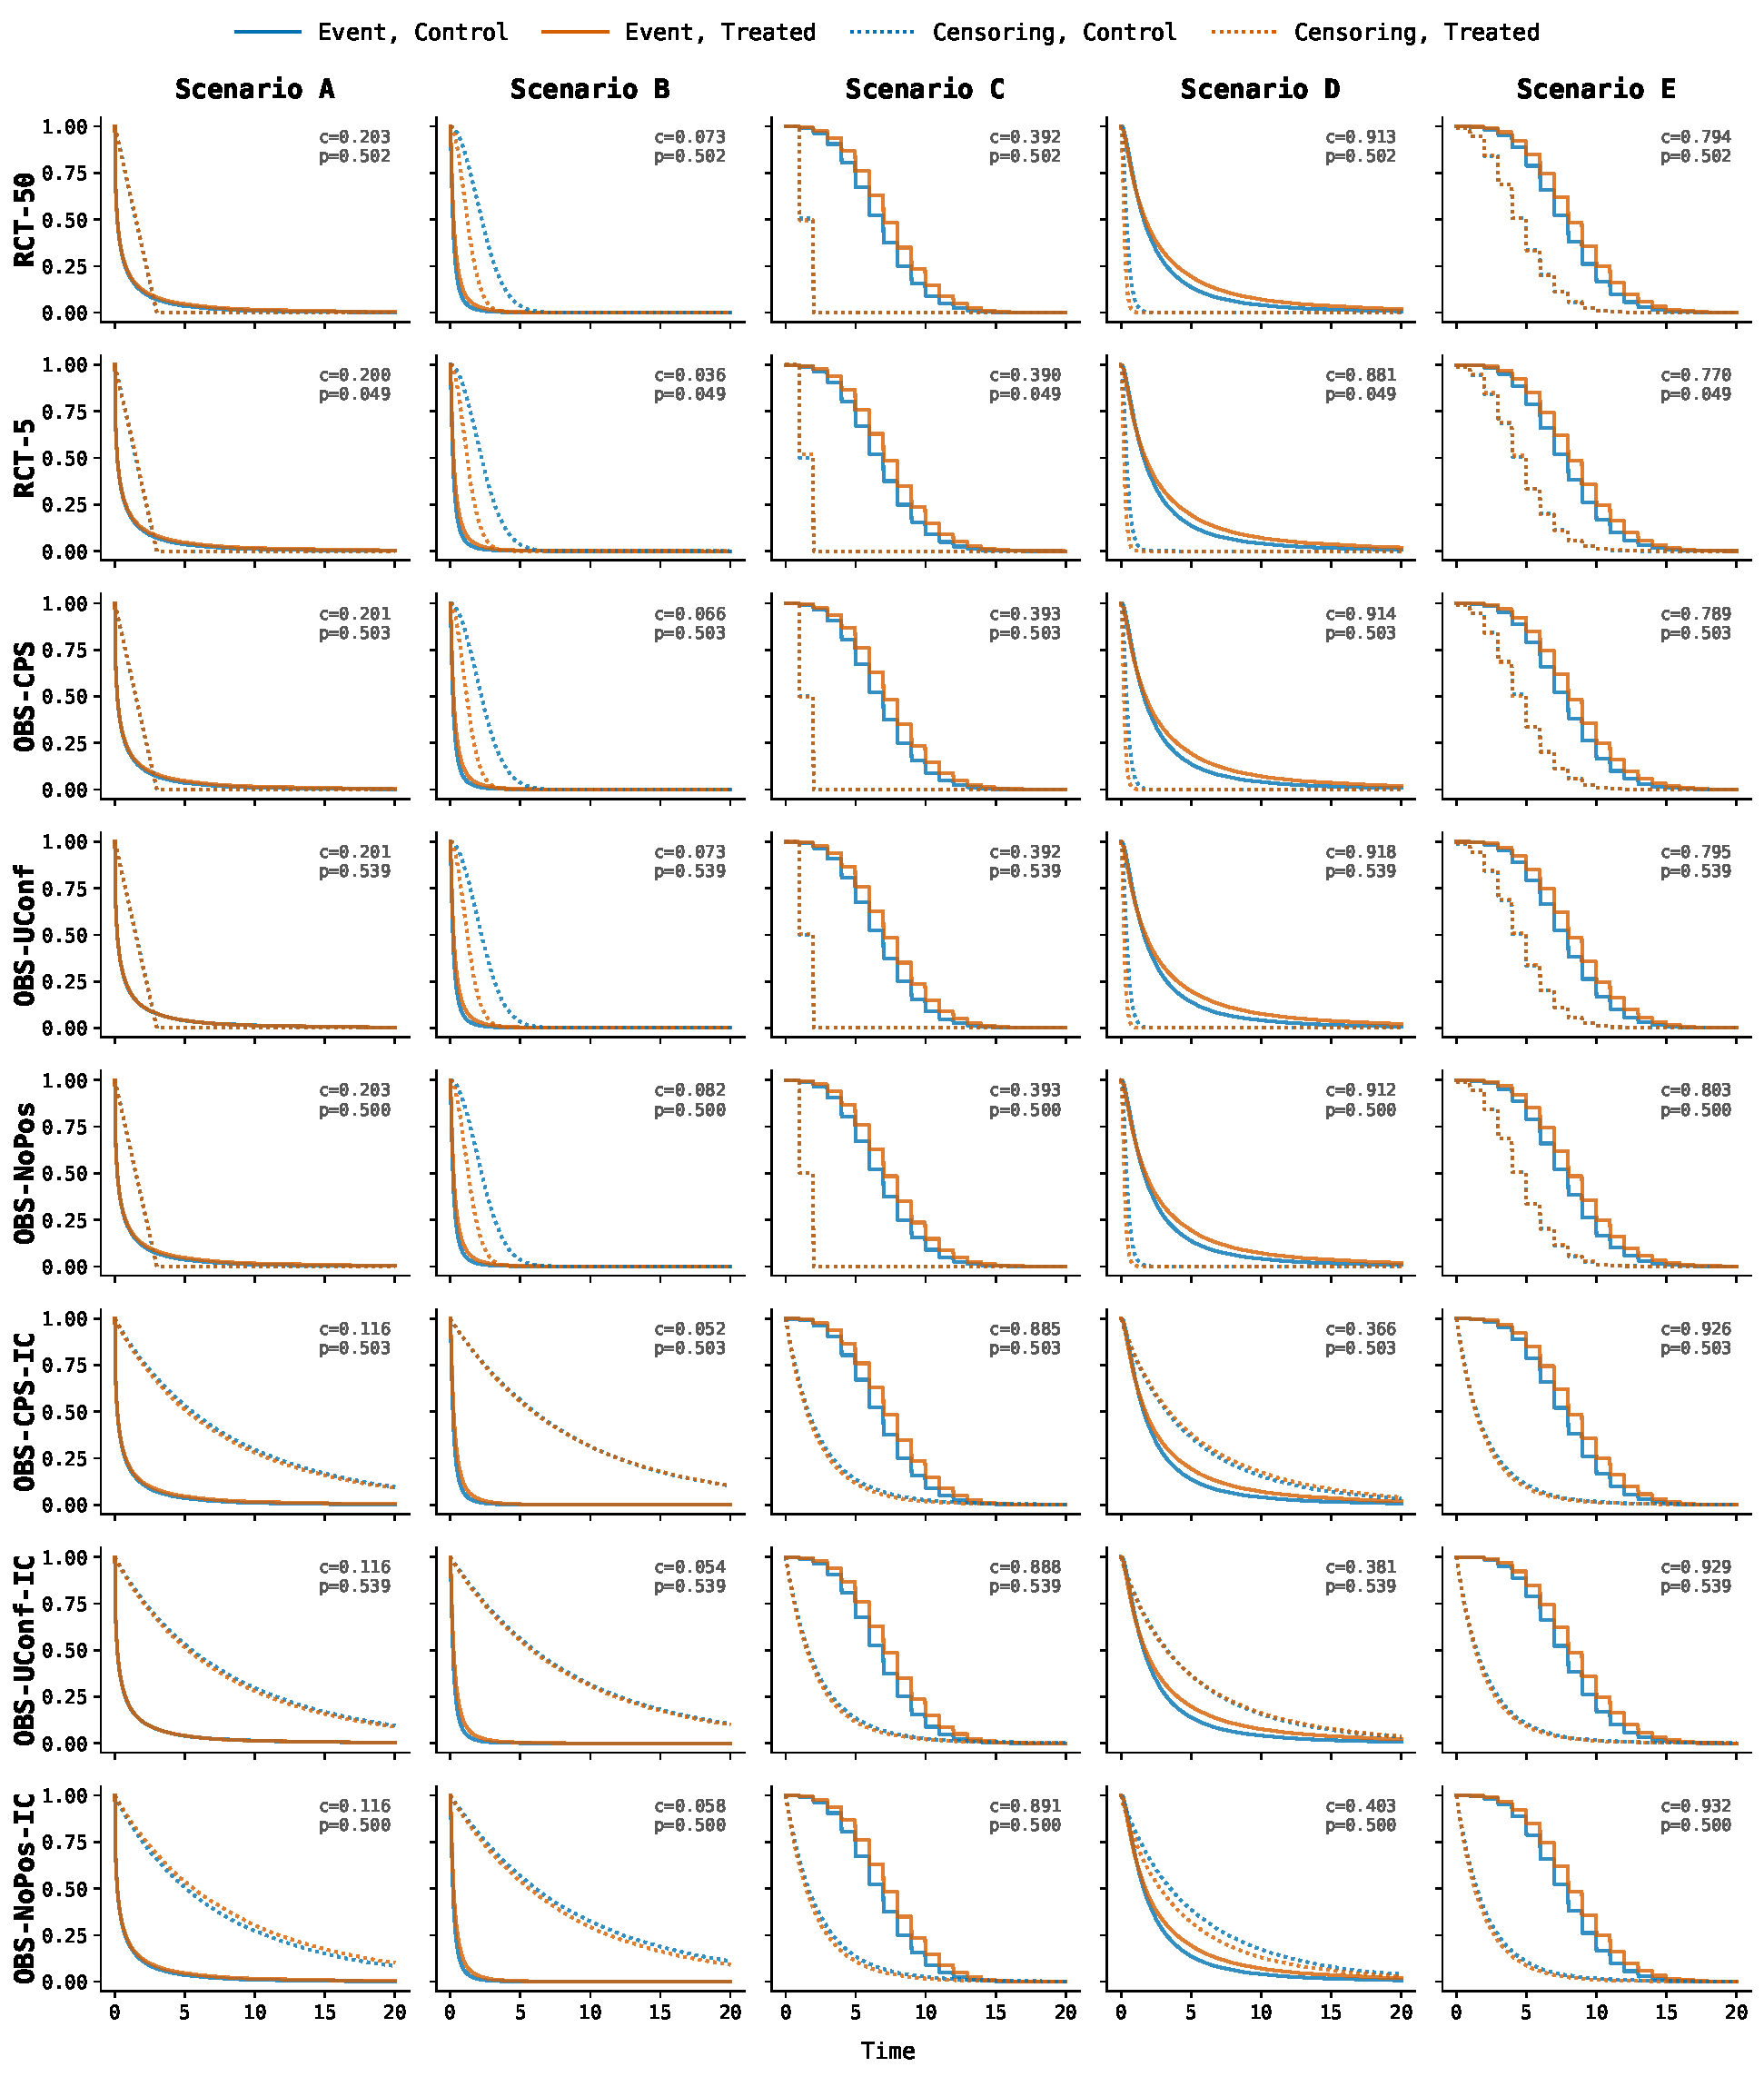
\includegraphics[width=1.0\linewidth]{Appendices/appendix-ch04/images/figure_results_updated/synthetic-km-curves.pdf} 
   
}
\end{figure}





\ChFourParagraph{\ChFourRebuttal{Remark on parameter calibration.}}
\ChFourRebuttal{The constants used in our synthetic generators are inherited from and aligned with prior causal-survival simulation setups~\citep{ch04:cui2023estimating,meir2025heterogeneous}, and are set to span distinct, interpretable regimes that the benchmark aims to cover. In particular, we calibrate (i) \emph{censoring severity} by shifting the relative scales of event-time and censoring-time processes (e.g., the AFT intercept change between Scenarios~\texttt{B} and~\texttt{D} increases typical event times and, together with the corresponding censoring model, yields higher censoring in \texttt{D}); (ii) \emph{treatment prevalence} and \emph{confounding strength} by adjusting propensity-score weights so that most configurations remain near balanced treatment except where imbalance is intentional (e.g., \texttt{RCT-5}), while allowing controlled dependence on observed or latent drivers; and (iii) \emph{effect magnitude/heterogeneity} through the coefficients on $W$ and $W$--covariate interactions, which we keep in a moderate range for comparability across scenarios. These choices are not unique, and alternative parameterizations could yield valid benchmarks; our goal is to provide a principled and reproducible instantiation that cleanly separates survival dynamics from causal-assumption stress and produces a broad range of survival CATE evaluation settings.}





% !TeX root = ../../../main.tex
\subsection{Imputation Methods Details} \label{ch04:app:imputation}

We follow \citet{qi2023an} to implement three surrogate imputation strategies for estimating the true event time \( T \) in right-censored survival data. Let \( Y = \min(T, C) \) be the observed time, with censoring indicator \( \delta = \mathbbm{1}\{T \leq C\} \). Let \( S_{\text{KM}(\mathcal{D})}(t) \) denote the Kaplan-Meier estimate of the survival function using the dataset \( \mathcal{D} \), and \( N \) the number of subjects. The three methods below are used to impute a surrogate outcome \( \tilde{T}_i \) for censored subject \( i \) observed at time \( t_i \).

\ChFourParagraph{1. Margin imputation:}
This method assigns a “best guess” value to each censored subject using the nonparametric Kaplan-Meier estimator. This surrogate value, called the \emph{margin time}, can be interpreted as the conditional expectation of the event time given that the event occurs after the censoring time. For a subject censored at time \( t_i \), the margin-imputed event time is computed as:
\begin{equation}
\tilde{T}^{\text{margin}}_i 
= \mathbb{E}[T_i \mid T_i > t_i] 
= t_i + \frac{\int_{t_i}^{\infty} S_{\text{KM}(\mathcal{D})}(t) \, dt}{S_{\text{KM}(\mathcal{D})}(t_i)}
\end{equation}
where \( S_{\text{KM}(\mathcal{D})}(t) \) is the Kaplan-Meier survival estimate derived from the training dataset.

The reliability of this imputation depends on the censoring time. For example, if a subject is censored very early (e.g., at time 0), the margin time is highly uncertain due to the lack of observed data beyond that point. In contrast, if a subject is censored near the maximum observed follow-up, the margin time is more likely to be close to the true event time.

\ChFourParagraph{2. IPCW-T imputation:}
This method imputes a surrogate event time for censored subjects based on the observed outcomes of subsequent uncensored individuals. Specifically, for a subject censored at time \( t_i \), the imputed value is calculated as the average event time of all uncensored subjects with observed times after \( t_i \):
\begin{equation}
\tilde{T}^{\text{IPCW}}_i = 
\frac{\sum_{j=1}^N \mathbbm{1}\{t_i < t_j\} \cdot \mathbbm{1}\{\delta_j = 1\} \cdot t_j}
     {\sum_{j=1}^N \mathbbm{1}\{t_i < t_j\} \cdot \mathbbm{1}\{\delta_j = 1\}}
\end{equation}
This imputes the event time for subject \( i \) by averaging the observed event times of those uncensored subjects who experienced the event after \( t_i \). The method is motivated by the idea that these subsequent subjects provide empirical evidence about the possible timing of the unobserved event.

However, a limitation of this approach is that it fails to provide an imputation when there are no uncensored subjects observed after \( t_i \). In such cases, the denominator of the expression becomes zero, and the method is unable to approximate the event time. In \citet{qi2023an}, subjects for whom this occurs are excluded from evaluation, whereas in our setup we used the original observed time as the imputed time.


\ChFourParagraph{3. Pseudo-observation imputation:}
This method imputes the event time using pseudo-observations, which estimate the contribution of each subject to an overall unbiased estimator of the event time distribution. Let \( \hat{\theta} \) be an estimator of the mean event time based on right-censored data, and let \( \hat{\theta}^{-i} \) denote the same estimator computed with the \( i \)-th subject removed from the dataset. Then, the pseudo-observation for subject \( i \) is defined as:
\begin{equation}
\tilde{T}^{\text{pseudo}}_i = e_{\text{Pseudo-Obs}}(t_i, \mathcal{D}) 
= N \cdot \hat{\theta} - (N - 1) \cdot \hat{\theta}^{-i}
\end{equation}
This quantity can be interpreted as the individual contribution of subject \( i \) to the overall estimate \( \hat{\theta} \). In practice, both \( \hat{\theta} \) and \( \hat{\theta}^{-i} \) can be computed using the mean of the Kaplan-Meier survival curve:
\[
\hat{\theta} = \mathbb{E}_t[S_{\text{KM}(\mathcal{D})}(t)], \quad
\hat{\theta}^{-i} = \mathbb{E}_t[S_{\text{KM}(\mathcal{D} \setminus \{i\})}(t)]
\]
Once the pseudo-observations \( \tilde{T}^{\text{pseudo}}_i \) are computed for all censored subjects, they are substituted in place of the true event times for evaluation or modeling. 

Although pseudo-observations are not exact conditional expectations, they can approximate \( \mathbb{E}[T_i \mid X_i] \) under certain assumptions. In particular, when censoring is independent of covariates and the sample size is large, pseudo-observations behave asymptotically like i.i.d. draws from the true conditional expectation:
\[
\mathbb{E}[\tilde{T}^{\text{pseudo}}_i \mid X_i] \approx \mathbb{E}[T_i \mid X_i]
\]
This makes the pseudo-observation method a principled, nonparametric approach for imputing censored survival times, particularly when estimating global quantities like the mean event time.

These imputation strategies enable us to transform the survival outcome into a fully observed target variable, allowing the application of standard regression-based methods in causal effect estimation. 
To ensure meaningful estimates, it is important that each imputed event time for a censored subject is guaranteed to be greater than or equal to the censoring time---reflecting the fact that the true event must occur after the last time it was observed. 
In our implementation, we manually enforce this constraint by setting the imputed value to the observed censoring time whenever the imputation procedure yields a value less than \( t_i \).

%%%%%%%%%%%%%%%%%%%%%%%%%%%%%%%%%%%%%%%%%%%%%%%%%%%%%%%%%%%%
%%%%%%%%%%%%%%%%%%%%%%%%%%%%%%%%%%%%%%%%%%%%%%%%%%%%%%%%%%%%
%%%%%%%%%%%%%%%%%%%%%%%%%%%%%%%%%%%%%%%%%%%%%%%%%%%%%%%%%%%%




% !TeX root = ../../../main.tex
\subsection{List of CATE Estimators in \textsc{SurvHTE} Benchmark} \label{ch04:app:exp-setup}


As mentioned in Section~\ref{ch04:sec:bench}, in our benchmark, we evaluate three families of survival CATE methods, totaling 53 variants.
We list the number of variants for each type of CATE estimator in Table~\ref{ch04:tab:baseline-details}.

For the outcome imputation methods, we first apply one of three imputation strategies (Pseudo-observation, Margin, or IPCW-T)~\citep{qi2023an} to handle the censored data, transforming the survival problem into a standard regression task.
After imputation, we use these imputed outcomes with four different meta-learner frameworks (S-, T-, X-, and DR-Learners), each implemented with three different base regression models (Lasso Regression, Random Forest, and XGBoost), resulting in $3 \times 4 \times 3 = 36$
different variants.
Additionally, we pair each imputation method with two specialized causal inference methods: Causal Forest~\citep{athey2019grf} and Double-ML~\citep{chernozhukov2018double}, which adds $3 \times 1 + 3 \times 1 = 6$ more variants, for a total of $42$ outcome imputation method variants.

For direct-survival CATE models, we include the Causal Survival Forests (CSF)~\citep{ch04:cui2023estimating} and SurvITE~\citep{curth2021survite}, which are specifically designed to handle right-censored data without requiring separate imputation steps.
SurvITE estimates individual treatment effects directly from right-censored survival data by learning balanced representations and optimizing a survival-specific loss.

For survival meta-learners, we implement three types of meta-learning frameworks that have been extended to handle censored data directly: S-Learner, T-Learner, and matching-learner~\citep{noroozizadeh2025impact}.
Each of these frameworks is combined with three different base survival models (Random Survival Forests~\citep{ch04:ishwaran2008random}, DeepSurv~\citep{ch04:katzman2018deepsurv}, and DeepHit~\citep{ch04:lee2018deephit}) that estimate the underlying survival functions, resulting in $3 \times 3 = 9$ survival meta-learner variants.

In total, our benchmark evaluates $42+2+9=53$ different method configurations across the 40 synthetic datasets and the two real-world datasets described in Section~\ref{ch04:sec:bench}.


% !TeX root = ../../../main.tex
\begin{table}[htbp]
\ChFourFloatContents{ch04:tab:baseline-details}{\caption{Breakdown of benchmarked survival-CATE estimator variants used in our experiments. 
    Each row corresponds to a specific combination of method class, imputation strategy (if applicable), base learner(s), and CATE learner(s). 
    Cells with numbers in parentheses indicate how many variants are contributed by the method(s) listed in that cell. 
    The final column reports the total number of method variants constructed using that combination. }}{
  \centering
  
  
  
  \begin{adjustbox}{max width = 0.85\textwidth}
  \renewcommand{\arraystretch}{1.8}\begin{tabular}{ccccc}
    \toprule
    \makecell{\textbf{Method Class}} &
    \makecell{\textbf{Imputation} \\ \textit{(No. options)}} &
    \makecell{\textbf{Base Learner} \\ \textit{(No. options)}} &
    \makecell{\textbf{CATE Learner} \\ \textit{(No. options)}} &
    \makecell{\textbf{No. Variants}} \\
    \midrule

    \multirow{3}{*}{\makecell[c]{Outcome\\Imputation\\Method}} 
      & \multirow{3}{*}{\makecell[c]{Pseudo-obs,\\Margin,\\IPCW-T\\\texttt{(3)}}}
      & \makecell[c]{Lasso Regression,\\Random Forest, XGBoost\\\texttt{(3)}} 
      & \makecell[c]{Meta-Learners\\ (S-, T-, X-, DR-)\\\texttt{(4)}} 
      & \textbf{36} \\
    \cmidrule(r){3-5}
    & ~
    & --- 
    & \makecell[c]{Causal Forest\\\texttt{(1)}}
    & \textbf{3} \\
    \cmidrule(r){3-5}
    & ~ 
    & --- 
    & \makecell[c]{Double-ML\\\texttt{(1)}}
    & \textbf{3} \\

    \midrule

    \makecell[c]{Direct-Survival \\CATE Models}
    & --- 
    & ---
    & \makecell[c]{Causal Survival Forests\\\texttt{(1)}\\SurvITE\\\texttt{(1)}}
    & \textbf{2} \\

    \midrule

    \makecell[c]{Survival \\ Meta-Learners} 
    & --- 
    & \makecell[c]{Random Survival Forests,\\DeepSurv, DeepHit\\\texttt{(3)}} 
    & \makecell[c]{Survival Meta-Learners\\ (S-, T-, Matching-)\\\texttt{(3)}} 
    & \textbf{9} \\

    \midrule

    \textbf{Total} 
    & 
    & 
    & 
    & \textbf{53} \\

    \bottomrule
  \end{tabular}
  \end{adjustbox}
}
\end{table}







% !TeX root = ../../../main.tex
\subsection{Detailed Overview of Causal Inference Methods}
\label{ch04:app:causal_method_details}

This section provides a comprehensive explanation of the causal inference methods evaluated in our benchmark.
We begin with outcome imputation methods that transform censored survival data into standard regression problems, followed by direct-survival CATE models specifically designed for right-censored data, and finally survival meta-learners that adapt standard meta-learner frameworks to handle censoring.
For each method, we present the theoretical foundation, algorithmic procedure, and specific implementation considerations in the survival analysis context.
Our exposition focuses on highlighting the unique characteristics that make each approach suitable for different survival and causal inference scenarios, with particular attention to how these methods handle the challenges posed by censoring and treatment effect heterogeneity.


\subsubsection{Outcome imputation methods}
Meta-learners represent a flexible framework for estimating conditional average treatment effects (CATEs) by decomposing the causal inference problem into standard supervised learning tasks.
The key advantage of meta-learners is that they allow practitioners to leverage any out-of-the-box machine learning algorithm as a ``base learner'' while maintaining principled approaches to causal effect estimation.
This modularity makes meta-learners particularly attractive in practice, as they can incorporate state-of-the-art ML methods (e.g., random forests, gradient boosting, neural networks) without requiring specialized causal inference implementations.
For detailed explanations on meta-learners, one can refer to \citet{ch04:kunzel2019metalearners,kennedy2023towards}.
We provide a simplified overview below and largely refer to the documentation of the \href{https://econml.azurewebsites.net/spec/spec.html}{\texttt{econml}} package.

\textbf{T-Learner \citep{ch04:kunzel2019metalearners}.}
The T-Learner (Two-Learner) adopts the most straightforward approach by fitting separate outcome models for treated and control groups.
Given binary treatment $W \in \{0,1\}$, features $X$, and outcome $Y$, the T-Learner:

\begin{enumerate}
    \item Splits the data by treatment assignment: ${(X^0, Y^0)}$ for controls and ${(X^1, Y^1)}$ for treated units
    \item Trains separate outcome models (i.e. predicting the outcome $Y$ using features $X$): 
        \begin{align*}
            \text{For control units: } \hat{\mu}_0 = M_0(Y^0 \sim X^0)\\
            \text{For treated units: } \hat{\mu}_1 = M_1(Y^1 \sim X^1)
        \end{align*}
    \item Estimates CATE as:
        \begin{align*}
            \hat{\tau}(x) = \hat{\mu}_1(x) - \hat{\mu}_0(x)
        \end{align*}
\end{enumerate}
where $M_0$ and $M_1$ can be any regression algorithm.
The T-Learner is conceptually simple but can suffer from high variance when treatment groups have different sizes or when the outcome models extrapolate poorly to regions with limited overlap.

\textbf{S-Learner \citep{ch04:kunzel2019metalearners}.} The S-Learner (Single-Learner) takes a unified modeling approach by including treatment assignment as an additional feature. The procedure involves:

\begin{enumerate}
    \item Training a single model using all available data:
        \begin{align*}
            \hat{\mu} = M(Y \sim (X, W))    
        \end{align*}
    \item Estimating CATE as: 
        \begin{align*}
            \hat{\tau}(x) = \hat{\mu}(x, 1) - \hat{\mu}(x, 0)
        \end{align*}
\end{enumerate}
This approach leverages all available data for training and can be more sample-efficient than the T-Learner.
However, it relies heavily on the base learner's ability to capture treatment-feature interactions, and may perform poorly when these interactions are complex or when the treatment effect is small relative to the baseline outcome.

\textbf{X-Learner \citep{ch04:kunzel2019metalearners}.} The X-Learner represents a more sophisticated approach that combines ideas from both T-Learner and inverse propensity weighting. The algorithm proceeds in multiple stages:
\begin{enumerate}
    \item Fit initial outcome models:
        \begin{align*}
            \hat{\mu}_0 = M_1(Y^0 \sim X^0)\\
            \hat{\mu}_1 = M_2(Y^1 \sim X^1)
        \end{align*}
    \item Compute imputed treatment effects:
        \begin{align*}
            \text{For treated units: } \hat{D}^1 = Y^1 - \hat{\mu}_0(X^1) \\
            \text{For control units: } \hat{D}^0 = \hat{\mu}_1(X^0) - Y^0
        \end{align*}
    \item Model treatment effects: 
        \begin{align*}
            \hat{\tau}_0 = M_3(\hat{D}^0 \sim X^0)\\ 
            \hat{\tau}_1 = M_4(\hat{D}^1 \sim X^1)
        \end{align*}
    \item Combine estimates using propensity scores: 
        \begin{align*}
            \hat{\tau}(x) = g(x)\hat{\tau}_0(x) + (1-g(x))\hat{\tau}_1(x)
        \end{align*}
\end{enumerate}
where $g(x)$ is the estimation for propensity score $P(W=1|X=x)$ and is typically fitted using logistic regression.
The X-Learner is particularly effective when treatment groups have different sizes or when treatment effects are heterogeneous, as it explicitly models treatment effect variation and uses propensity weighting for optimal combination.

\textbf{DR-Learner \citep{kennedy2023towards}}. The DR-Learner (Doubly Robust Learner) extends the doubly robust framework to meta-learning by combining outcome modeling with propensity score estimation. The approach constructs doubly robust scores that remain consistent if either the outcome model or propensity model is correctly specified. It includes the following steps:
\begin{enumerate}
    \item Fit outcome modeling for each treatment
        \begin{align*}
            \hat{\mu}_0 = M_1(Y^0 \sim X^0)\\
            \hat{\mu}_1 = M_2(Y^1 \sim X^1)
        \end{align*}
    \item Construct propensity score modeling
        \begin{align*}
            \hat{g} = M_g(W \sim X)
        \end{align*}
    \item Construct doubly robust outcomes:
        \begin{align*}
            \hat{Y}_{0}^{DR} = \hat{\mu}_0(X) + \frac{(Y - \hat{\mu}_0(X))}{\hat{g}(X)}  \cdot \ChFourInd\{W = 0\} \\
            \hat{Y}_{1}^{DR} = \hat{\mu}_1(X) + \frac{(Y - \hat{\mu}_1(X))}{\hat{g}(X)}  \cdot \ChFourInd\{W = 1\}
        \end{align*}
    \item Final CATE estimation: $\hat{\tau}(x) = \hat{Y}_{1}^{DR} - \hat{Y}_{0}^{DR}$
\end{enumerate}
The DR-Learner provides theoretical robustness guarantees and often performs well in practice, particularly when either outcome or treatment assignment can be accurately modeled.

\textbf{Double-ML \citep{chernozhukov2018double}.} Double Machine Learning (Double-ML or DML) represents a principled framework for estimating heterogeneous treatment effects when confounders are high-dimensional or when their relationships with treatment and outcome cannot be adequately captured by parametric models. The key insight of DML is to decompose the causal inference problem into two predictive tasks that can be solved using arbitrary machine learning algorithms while maintaining favorable statistical properties. Specifically, DML assumes the following structural relationships:
\begin{itemize}
    \item $Y = \theta(X) \cdot W + g(X, Z) + \epsilon \quad \text{with} \quad \mathbb{E}[\epsilon | X, Z] = 0$
    \item $W = f(X, Z) + \eta \quad \text{with} \quad \mathbb{E}[\eta | X, Z] = 0$
    \item $\mathbb{E}[\eta \cdot \epsilon | X, Z] = 0$
\end{itemize}
where $Y$ is the outcome, $W$ is the treatment, $X$ are the features of interest for heterogeneity, $Z$ are confounding variables, and $\theta(X)$ is the conditional average treatment effect we aim to estimate.
The method proceeds by first estimating two nuisance functions:
\begin{itemize}
    \item Outcome regression: $q(X, Z) = \mathbb{E}[Y | X, Z]$
    \item Treatment regression: $f(X, Z) = \mathbb{E}[W | X, Z]$
\end{itemize}
These nuisance functions can be estimated using any machine learning algorithm capable of regression (for continuous treatments) or classification (for binary treatments).
Popular choices include random forests, gradient boosting, neural networks, or regularized linear models.
After obtaining estimates $\hat{q}$ and $\hat{f}$, DML constructs residualized outcomes and treatments:
\begin{align*}
    \tilde{Y} = Y - \hat{q}(X, Z)\\
    \tilde{W} = W - \hat{f}(X, Z)
\end{align*}

The final step estimates $\theta(X)$ by regressing $\tilde{Y}$ on $\tilde{W}$ and $X$
\begin{align*}
    \hat{\theta} = \arg\min_{\theta} \mathbb{E}_n[(\tilde{Y} - \theta(X) \cdot \tilde{W})^2]    
\end{align*}


\textbf{Causal Forest \citep{athey2019grf}.} Causal Forest extends the random forest methodology to directly estimate heterogeneous treatment effects in a non-parametric, data-adaptive manner. Unlike meta-learners that rely on global models, Causal Forest estimates treatment effects locally by learning similarity metrics in the feature space and weighting observations accordingly. Causal Forest builds upon the same structural assumptions as DML but estimates $\theta(x)$ locally for each target point $x$. The method constructs a forest where each tree is grown using a \textbf{causal splitting criterion} that maximizes treatment effect heterogeneity rather than prediction accuracy. For a target point $x$, the treatment effect is estimated by solving:
\begin{align*}
    \hat{\theta}(x) = \arg\min_{\theta} \sum_{i=1}^n K_x(X_i) \cdot (\tilde{Y}_i - \theta \cdot \tilde{W}_i)^2
\end{align*}
where $K_x(X_i)$ represents the similarity between points $x$ and $X_i$ as determined by how frequently they fall in the same leaf across the forest, and $\tilde{Y}$, $\tilde{W}$ are residuals from nuisance function estimates.

\textbf{Implementation in survival context}
In our benchmark, meta-learners, Double-ML, and Causal Forest are applied to survival outcomes through outcome imputation methods.
We first apply imputation techniques (Pseudo-obs, Margin, or IPCW-T, see Appendix~\ref{ch04:app:imputation} for details) to convert censored survival times into continuous outcomes, then apply the meta-learners described above with various base regression algorithms (Lasso Regression, Random Forest, XGBoost).
This two-stage approach allows leveraging the rich ecosystem of causal inference methods developed for continuous outcomes while handling the complexities of censored data.

\subsubsection{Direct-survival CATE methods}
\textbf{Causal Survival Forests (CSF) \citep{ch04:cui2023estimating}} extends the Causal Forest methodology directly to right-censored survival data by incorporating doubly robust estimating equations from survival analysis. Unlike meta-learners that require outcome imputation, CSF handles censored observations natively while maintaining the adaptive partitioning advantages of tree-based methods.
CSF builds upon the Causal Forest framework of \citet{athey2019grf} but adapts the splitting criterion and estimation procedure for survival outcomes.
For a detailed explanation of the method, please refer to the original paper by \citet{ch04:cui2023estimating}.
We provide an overview of the estimation procedures as follows:
\begin{enumerate}
    \item \textbf{Nuisance estimation}: Using cross-fitting, estimate nuisance components including:
        \begin{itemize}
            \item Propensity scores: $\hat{e}(x) = P(W = 1|X = x)$
            \item Outcome regression: $\hat{m}(x) = E[y(T)|X = x]$ 
            \item Censoring survival function: $\hat{S}^C_w(s|x) = P(C \geq s|W = w, X = x)$
            \item Conditional expectations: $\hat{Q}_w(s|x) = E[y(T)|X = x, W = w, T \wedge h > s]$
        \end{itemize}
        where $y(T)$ is a transformation applied on the event time $T$, the same as defined in Eq.\ref{ch04:eq:cate}.
    \item \textbf{Forest construction}: Build a forest where each tree uses a causal splitting criterion that maximizes treatment effect heterogeneity.
The splitting rule targets variation in the doubly robust scores rather than prediction accuracy.
    \item \textbf{Local estimation}: For a target point $x$, compute forest weights $\alpha(x)$ indicating similarity based on leaf co-occurrence across trees, then estimate the CATE by solving:
        \begin{align*}
            \sum \alpha(x) \psi_{\hat{\tau}(x)}(X, y(U), U \wedge h, W, \Delta^h; \hat{e}, \hat{m}, \hat{S}^C_w, \hat{Q}_w) = 0
        \end{align*}
        where $\psi$ is the doubly robust score function that adjusts for both treatment assignment and censoring.
\end{enumerate}


\textbf{SurvITE \citep{curth2021survite}} adapts the representation learning paradigm for counterfactual inference to time-to-event data. Unlike methods that rely on local similarity in the covariate space, SurvITE addresses selection bias by learning a shared latent representation where the treated and control distributions are balanced, while simultaneously modeling the censoring mechanism.
SurvITE builds upon the theoretical bounds of counterfactual regression but incorporates survival-specific loss functions to handle right-censored outcomes without requiring imputation.
A brief outline of the method follows:
\begin{enumerate}
    \item \textbf{Representation learning}: Map covariates $X$ to a latent representation $\Phi(X)$ via a deep neural network, subject to a discrepancy penalty.
The objective is to minimize an Integral Probability Metric (IPM) (e.g., Wasserstein distance or MMD) between the treated and control populations in the latent space:
        \begin{align*}
            \text{IPM}(P_{\Phi}(X|W=1), P_{\Phi}(X|W=0)) < \epsilon
        \end{align*}
    \item \textbf{Factual loss minimization}: Simultaneously train treatment-specific hypothesis heads ($h_1$ and $h_0$) on top of $\Phi(X)$ using a survival loss function $\mathcal{L}_{surv}$ (discrete-time log-likelihood) that accounts for censoring:
        \begin{align*}
            \min_{\Phi, h_0, h_1} \sum_{i=1}^N w_i \mathcal{L}_{surv}(h_{W_i}(\Phi(x_i)), T_i, \Delta_i) + \alpha \cdot \text{IPM}
        \end{align*}
    \item \textbf{Effect estimation}: For a target point $x$, the CATE is estimated by passing $x$ through the learned representation and computing the difference between the outputs of the treatment and control heads:
        \begin{align*}
             \hat{\tau}(x) = E[y(T)|\Phi(x), W=1] - E[y(T)|\Phi(x), W=0]
        \end{align*}
        where the expectation is derived from the predicted survival curves or time-to-event distributions output by $h_1$ and $h_0$.
\end{enumerate}


\subsubsection{Survival Meta-Learners}

\textbf{T-Learner-Survival \citep{bo2024ameta,noroozizadeh2025impact}.}
The T-Learner can be adapted to right-censored survival data by fitting separate survival models for each treatment group.
Let $W \in \{0, 1\}$ denote the treatment indicator, $X$ be the covariate vector, and $T$ the observed survival time with censoring indicator $\delta$, and $h$ the maximum follow-up time.

\begin{enumerate}
    \item \textbf{Split data by treatment:} Partition the dataset into $(X^0, T^0, \delta^0)$ for $W=0$ and $(X^1, T^1, \delta^1)$ for $W=1$.
    \item \textbf{Train separate survival models:} Fit a survival model (e.g., Random Survival Forests, DeepSurv, DeepHit) to each group:
    \begin{align*}
        \widehat{S}_0(u | x) &= \text{Survival model fitted on } (X^0, T^0, \delta^0) \\
        \widehat{S}_1(u | x) &= \text{Survival model fitted on } (X^1, T^1, \delta^1)
    \end{align*}
    \item \textbf{Estimate restricted mean survival time (RMST):} Compute RMST for each treatment as:
    \begin{align*}
        \widehat{\mu}_0(x) = \int_0^h \widehat{S}_0(u|x) du, \quad \widehat{\mu}_1(x) = \int_0^h \widehat{S}_1(u|x) du
    \end{align*}
    \item \textbf{Estimate CATE:} For any $x$, estimate treatment effect:
    \begin{align*}
        \widehat{\tau}_{\text{T-Learner}}(x) = \widehat{\mu}_1(x) - \widehat{\mu}_0(x)
    \end{align*}
\end{enumerate}

\textbf{S-Learner-Survival \citep{bo2024ameta,noroozizadeh2025impact}.}
The S-Learner adapts by training a single survival model over all data with treatment as a covariate.

\begin{enumerate}
    \item \textbf{Fit survival model:} Train a survival model over the full dataset using $(X, W)$ as inputs:
    \begin{align*}
        \widehat{S}(u | x, w) = \text{Survival model fitted on } ((X, W), T, \delta)
    \end{align*}
    \item \textbf{Estimate restricted mean survival time (RMST):} Compute RMST under both treatment conditions:
    \begin{align*}
        \widehat{\mu}(x, 0) = \int_0^h \widehat{S}(u|x, 0) du, \quad \widehat{\mu}(x, 1) = \int_0^h \widehat{S}(u|x, 1) du
    \end{align*}
    \item \textbf{Estimate CATE:} 
    \begin{align*}
        \widehat{\tau}_{\text{S-Learner}}(x) = \widehat{\mu}(x,1) - \widehat{\mu}(x,0)
    \end{align*}
\end{enumerate}

\textbf{Matching-Survival \citep{noroozizadeh2025impact}.}
The Matching-Learner estimates the CATE by imputing the counterfactual Restricted Mean Survival Time (RMST) using matched data points from the opposite treatment group.

\begin{enumerate}
    \item \textbf{Estimate factual RMST:} Fit a survival model on the full dataset and compute:
    \begin{align*}
        \widehat{\mu}_{W_i}(X_i) = \int_0^h \widehat{S}(u | X_i, W_i) du
    \end{align*}
    \item \textbf{Find matches:} For each individual $i$, identify $K$ nearest neighbors $J_K(i)$ from the opposite treatment group (\(1-W_i\)).
    \item \textbf{Estimate counterfactual RMST:} Average factual RMSTs of matched neighbors:
    \begin{align*}
        \widehat{\mu}_{1-W_i}(X_i) = \frac{1}{K} \sum_{j \in J_K(i)} \widehat{\mu}_{W_j}(X_j)
    \end{align*}
    \item \textbf{Estimate CATE:} Compute CATE for each unit:
    \begin{align*}
        \widehat{\tau}_{\text{matching}}(X_i) = \big(\widehat{\mu}_{W_i}(X_i) - \widehat{\mu}_{1-W_i} (X_i)\big) \cdot \big(2 W_i - 1 \big)
    \end{align*}
\end{enumerate}

This approach makes minimal modeling assumptions beyond nearest-neighbor similarity and is particularly helpful in settings with low overlap or where global models may be misspecified.





% !TeX root = ../../../main.tex
\subsection{Model Training Details and Hyperparameters on Benchmarking with Synthetic Data}
\label{ch04:app:method_settings}

To rigorously evaluate and compare the performance of causal inference models under controlled conditions, we conducted extensive benchmarking on synthetic datasets. Each synthetic dataset consisted of 50,000 samples generated under known data-generating processes explained in Appendix~\ref{ch04:app:synthetic-dataset}. For each experimental repeat, we selected a subset of 5,000 samples for training, 2,500 for validation, and 2,500 for testing, using 10 distinct random seeds (experimental repeats) to ensure robustness. Hyperparameters for each model were tuned on the validation set to minimize the Conditional Average Treatment Effect Root Mean Squared Error (CATE-RMSE).
Throughout this paper, final results are always reported on the held-out test set using the best-performing configuration. Appendix~\ref{ch04:app:varying-train-size} provides complementary experiments that analyze the convergence behavior of each method under varying training set sizes.

This appendix details the hyperparameter grids used for model selection, the specific survival and outcome models applied within each causal inference framework, and the average computational cost associated with each method class.


\subsubsection{Hyperparameters for outcome imputation methods}

For methods based on outcome imputation, we employed standard regressors to estimate the conditional mean of the survival outcome given covariates and treatment assignment. We considered Lasso regression, Random Forest, and XGBoost as base models. Each was optimized using cross-validated grid search on the training set. The corresponding hyperparameter grids are listed in Table~\ref{ch04:tab:hyperparam-outcome-impute-reg}.


% !TeX root = ../../../main.tex
\begin{table}[htbp]
\ChFourFloatContents{ch04:tab:hyperparam-outcome-impute-reg}{\caption{Set of hyperparameters for outcome imputation methods}}{
\centering
\footnotesize
\setlength{\tabcolsep}{4pt}
% \captionsetup{labelformat=empty}
 
\begin{tabular}{l l}
\toprule
\textbf{Regressor} & \textbf{Hyperparameter Grid} \\ \midrule
Lasso & Alpha: \{0.001, 0.01, 0.1, 1, 10\} \\ \midrule
Random Forest & 
\begin{tabular}[t]{@{}l@{}}
Number of trees: \{50, 100\} \\
Maximum depth: \{3, 5, None\}
\end{tabular} \\ \midrule
XGBoost & 
\begin{tabular}[t]{@{}l@{}}
Number of trees: \{50, 100\} \\
Learning rate: \{0.01, 0.1\} \\
Maximum depth: \{3, 5\}
\end{tabular} \\
\bottomrule
\end{tabular}
}
\end{table}




\subsubsection{Hyperparameters for direct-survival CATE methods}

For direct modeling of survival outcomes, we employed the Causal Survival Forests (CSF), which adapts the Causal Forest framework to handle right-censored data. We used the default hyperparameters from the original implementation. These are summarized in Table~\ref{ch04:tab:hyperparam-csf}.


% !TeX root = ../../../main.tex
\begin{table}[htbp]
\ChFourFloatContents{ch04:tab:hyperparam-csf}{\caption{Set of hyperparameters for Causal Survival Forests}}{
\centering
\footnotesize
\setlength{\tabcolsep}{4pt}
% \captionsetup{labelformat=empty}
 
\begin{tabular}{l l}
\toprule
\textbf{Parameter} & \textbf{Default Value} \\ \midrule
Number of trees grown & 2000 \\
Fraction of data per tree & 0.5 \\
Variables tried per split & $\min(\lceil\sqrt{p}+20\rceil, p)$ \\
Minimum samples in a leaf & 5 \\
Maximum imbalance of splits & 0.05 \\
Penalty for imbalance at split & 0 \\
Account for treatment and censoring in split stability & TRUE \\
Trees per subsample for confidence intervals & 2 \\
\bottomrule
\end{tabular}
}
\end{table}


For SurvITE, we implemented a PyTorch version based on the original architecture and repository. The main configuration is summarized in Table~\ref{ch04:tab:hyperparam-survite}. % Unless otherwise noted, we use the same settings for all datasets. For datasets with \texttt{mimic\_syn} we increase the hidden layer widths to $64$ units to accommodate the higher-dimensional feature space.

% \begin{table}[htbp]
% \centering
% \footnotesize
% \setlength{\tabcolsep}{4pt}
% \caption{\rebuttal{Hyperparameters for SurvITE \textcolor{red}{Polish the text in this table; update hyperparameters}}}
% \label{tab:hyperparam-survite}
% \begin{tabular}{l l}
% \toprule
% \textbf{Parameter} & \textbf{Value} \\ \midrule
% Latent representation dimension $z\_\text{dim}$ & Same as Head hidden dimensions (see below) \\
% Shared hidden layer width $h\_\text{dim1}$ & Same as Head hidden dimensions (see below) \\
% Head hidden layer width $h\_\text{dim2}$ & $\{8,16,32,64\}$ for synthetic, ACTG semi-synthetic, and ACTG datasets,  or $\{16,32,64,128\}$ for MIMIC semi-synthetic and twin datasets\\
% Number of shared layers $\text{num\_layers1}$ & 2 \\
% Number of head layers $\text{num\_layers2}$ & 2 \\
% Activation function & ReLU \\
% Dropout rate & 0.3 \\
% IPM type & Wasserstein \\
% IPM regularization weight $\beta$ & $10^{-3}$ \\
% Smoothing parameter $\gamma$ & 0 \\
% Learning rate & $10^{-3}$ \\
% Batch size & 256 \\
% Maximum epochs & 5000 \\
% Early stopping patience & 10 (checked every 100 epochs) \\
% \bottomrule
% \end{tabular}
% \end{table}
% }


% !TeX root = ../../../main.tex
\begin{table}[htbp]
\ChFourFloatContents{ch04:tab:hyperparam-survite}{\caption{Set of hyperparameters SurvITE.}}{
\centering
\footnotesize
\setlength{\tabcolsep}{4pt}


\begin{tabular}{l l}
\toprule
\textbf{Parameter} & \textbf{Value} \\ 
\midrule
Model width $z_{\text{dim}}, h_{\text{dim1}}, h_{\text{dim2}}$
& $\{8,16,32\}$ (synthetic, ACTG) or $\{16,32,64\}$ (MIMIC, Twin) \\
Number of shared layers & 2 \\
Number of head layers & 2 \\
Activation function & ReLU \\
Dropout rate & 0.3 \\
IPM type & Wasserstein \\
IPM regularization weight $\beta$ & $10^{-3}$ \\
Smoothing parameter $\gamma$ & 0 \\
Learning rate & $10^{-3}$ \\
Batch size & 256 \\
Maximum epochs & 5000 \\
Early stopping & Checked every 100 epochs; stop after 10 non-improving checks \\
\bottomrule
\end{tabular}
}
\end{table}




\subsubsection{Hyperparameters for survival meta-learners}

{\raggedright For survival meta-learners--specifically T-Learner-Survival, S-Learner-Survival, and Matching-\allowbreak Learner-Survival--we used three different base survival models: Random Survival Forests (RSF), DeepSurv, and DeepHit. Each of these models was tuned using a predefined hyperparameter grid, listed in Table~\ref{ch04:tab:hyperparam-base-surv}.\par}


% !TeX root = ../../../main.tex
\begin{table}[htbp]
\ChFourFloatContents{ch04:tab:hyperparam-base-surv}{\caption{Set of hyperparameters for Survival Meta-Learners}}{
\centering
\footnotesize
\setlength{\tabcolsep}{4pt}
 
\begin{adjustbox}{max width = 0.55\textwidth}
\begin{tabular}{l l c}
\toprule
\textbf{Model}         & \textbf{Hyperparameter}             & \textbf{Values} \\ \midrule
\multirow{3}{*}{RSF}   & Number of estimators                & \{100, 250, 500\}   \\
                       & Minimum samples per split           & \{5, 10, 20\}       \\
                       & Minimum samples per leaf            & \{2, 5, 10\}        \\ \midrule
\multirow{8}{*}{DeepHit} 
                       & Number of nodes per layer           & \{32, 64, 128, 256\} \\
                       & Batch normalization                 & \{True, False\}       \\
                       & Dropout rate                        & \{0.0, 0.1, 0.2, 0.3\} \\
                       & Learning rate                       & \{0.001, 0.01, 0.05\} \\
                       & Batch size                          & \{128, 256, 512\}    \\
                       & Epochs                              & \{200, 512, 1000\}   \\
                       & Alpha                               & \{0.1, 0.2, 0.3, 0.5\} \\
                       & Sigma                               & \{0.05, 0.1, 0.2, 0.3\} \\ \midrule
\multirow{6}{*}{DeepSurv} 
                       & Number of nodes per layer           & \{32, 64, 128, 256\} \\
                       & Batch normalization                 & \{True, False\}       \\
                       & Dropout rate                        & \{0.0, 0.1, 0.2, 0.3\} \\
                       & Learning rate                       & \{0.001, 0.01, 0.05\} \\
                       & Batch size                          & \{128, 256, 512\}    \\
                       & Epochs                              & \{200, 512, 1000\}   \\ \bottomrule
\end{tabular}
\end{adjustbox}
}
\end{table}


Hyperparameters were selected through empirical tuning informed by prior literature. For neural network-based models (DeepSurv, DeepHit), we used early stopping to mitigate overfitting. All experiments were made reproducible by setting random seeds. The best-performing hyperparameter configuration was selected using CATE-RMSE on the validation set, and all final results were obtained on the test set using these optimal configurations.


\subsubsection{Computation time of survival CATE methods}

We also measured the computational cost of each CATE estimation method in terms of average runtime per dataset and experimental repeat. Each runtime was recorded using Python’s \texttt{time.time()} and averaged across 40 synthetic datasets and 10 random seeds. Table~\ref{ch04:tab:runtime-comparison} presents the mean runtime (in seconds) and standard deviation (excluding the time required for imputation). 
As expected, neural network-based survival models incur substantially higher computational costs than classical or tree-based methods. All experiments were conducted on a machine equipped with an AMD Ryzen 9 5900X CPU, 128GB RAM, and an NVIDIA GeForce RTX 4090 GPU (CUDA version 12.2).


% !TeX root = ../../../main.tex
\begin{table}[htbp]
\ChFourFloatContents{ch04:tab:runtime-comparison}{\caption{Average computation time per dataset per experimental repeat for each causal method. Runtime is reported in seconds with standard deviation across runs.}}{
  \centering
  \footnotesize
  
  
  
  \begin{adjustbox}{max width = 0.6\textwidth}
  \begin{tabular}{lll}
    \toprule
    \textbf{Method Class} & \textbf{Method} & \textbf{Runtime (s)} \\
    \midrule

    \multirow{4}{*}{\makecell[l]{Outcome Imputation Methods: \\ Meta-learners}} 
      & T-Learner & 2.14 $\pm$ 1.38 \\
      & S-Learner & 1.84 $\pm$ 1.22 \\
      & X-Learner & 2.92 $\pm$ 2.42 \\
      & DR-Learner & 3.34 $\pm$ 1.88 \\

    \midrule

    \multirow{2}{*}{\makecell[l]{Outcome Imputation Methods: \\ Forest / ML-based learners}} 
      & Double-ML & 5.27 $\pm$ 0.40 \\
      & Causal Forest & 5.75 $\pm$ 0.40 \\

    \midrule

    \multirow{2}{*}{\makecell[l]{Direct-Survival CATE Methods}} 
    & Causal Survival Forests & 0.78 $\pm$ 0.06 \\
    & SurvITE &  43.15 $\pm$ 6.85 \\

    \midrule

    \multirow{3}{*}{Survival Meta-Learners} 
      & T-Learner-Survival & 31.31 $\pm$ 16.88 \\
      & S-Learner-Survival & 22.99 $\pm$ 14.23 \\
      & Matching-Survival & 49.40 $\pm$ 23.25 \\

    \bottomrule
  \end{tabular}
  \end{adjustbox}
}
\end{table}





%%%%%%%%%%%%%%%%%%%%%%%%%%%%%%%%%%%%%%%%%%%%%%%%%%%%%%%%%%%%
%%%%%%%%%%%%%%%%%%%%%%%%%%%%%%%%%%%%%%%%%%%%%%%%%%%%%%%%%%%%
%%%%%%%%%%%%%%%%%%%%%%%%%%%%%%%%%%%%%%%%%%%%%%%%%%%%%%%%%%%%


% !TeX root = ../../../main.tex
\ChFourLongSection{Additional Experimental Results for Synthetic Dataset}
\label{ch04:app:additional_synthetic_exps}

This section provides comprehensive experimental results on our synthetic datasets, expanding on the key findings presented in the main text.
We begin in Appendix~\ref{ch04:app:full-rankings} with a full Borda ranking of all 53 model combinations, summarizing global performance across every causal configuration and survival scenario.
In Appendix~\ref{ch04:app:average_rank_per_scenario}, we explore how performance varies across different survival scenarios--illustrating the impact of censoring patterns and time-to-event distributions on method rankings.
Appendix~\ref{ch04:app:more-avg-rank} then delves into how violations of causal assumptions (treatment randomization, ignorability, positivity, and censoring mechanisms) reshape the ranking of models for effectiveness of each causal method.

Subsequent sections (\ref{ch04:app:more-cate-mse-plots} and \ref{ch04:app:more-ate-plots}) present detailed performance metrics---CATE RMSE and ATE bias, respectively---across all 8 causal configurations and 5 survival scenarios, with box plots capturing variability over 10 experiment repetitions.
We also evaluate auxiliary components in \ref{ch04:app:auxiliary-eval-results}, including imputation methods and base learners (regression, survival, and propensity models), and in Appendix~\ref{ch04:app:varying-train-size} we examine convergence behavior under varying training set sizes.
Together, these detailed results support the robustness, sensitivity, and practical trade-offs of each model family in a wide spectrum of data-generating and causal settings.

\ChFourRebuttal{In addition to average-rank summaries, in Appendix~\ref{ch04:app:full-rankings}--~\ref{ch04:app:more-avg-rank}, we also report a set of win-rate analyses that track how often each method family attains Top-1, Top-3, and Top-5 performance on both \textcolor{black}{CATE RMSE and ATE Bias}. Overall win-rates across all survival scenarios and causal configurations are summarized in Table~\ref{ch04:tab:overall-winrate}, while Tables~\ref{ch04:tab:scenario-winrates},~\ref{ch04:tab:winrate-rct-configs}, and~\ref{ch04:tab:winrate-obs-configs} provide scenario-specific and causal-configuration-specific win-rates. These complementary views highlight not only which methods achieve strong average performance, but also which ones most consistently appear among the top performers across varying censoring regimes, survival experimental conditions, and patterns of causal assumption violations.}

\subsubsection{Full ranking of models}
\label{ch04:app:full-rankings}

To compare the overall performance of the methods across all synthetic datasets, we computed a Borda ranking based on the average rank of each method’s test set CATE RMSE (Table~\ref{ch04:tab:borda-rank-all-method}).
The ranking procedure aggregates method performance across all combinations of causal configurations and survival scenarios.
For each method, we first computed its RMSE on the test subset of the CATE predictions for each (causal configuration, survival scenario) pair.
We then ranked all \ChFourRebuttal{53} methods (described in Appendix~\ref{ch04:app:exp-setup}) within each pair and calculated the average rank across these conditions.
This average rank represents the method’s Borda score and serves as a unified summary of its performance robustness in our synthetic data experiments.


% !TeX root = ../../../main.tex
\begin{table}[htbp]
\ChFourFloatContents{ch04:tab:borda-rank-all-method}{\caption{\ChFourRebuttal{Borda ranking of all methods}}}{
\centering
 
\begin{adjustbox}{max width=\textwidth, center}
\begin{tabular}{rlr@{\hskip 24pt}rlr}
\toprule
\textbf{Rank} & \textbf{Method} & \textbf{Score} & \textbf{Rank} & \textbf{Method} & \textbf{Score} \\
\midrule
\textbf{1}  & (S-Learner-Survival, DeepSurv) & 5.18  & \textbf{28} & (Causal Forest, Pseudo-Obs) & 24.70 \\
\textbf{2}  & (Matching-Survival, DeepSurv) & 5.43  & \textbf{29} & (T-Learner, Margin, RandomForest) & 26.23 \\
\textbf{3}  & (Double-ML, Margin) & 6.65  & \textbf{30} & (S-Learner, IPCW-T, RandomForest) & 26.50 \\
\textbf{4}  & (Causal Forest, Margin) & 10.78 & \textbf{31} & (SurvITE) & 27.28 \\
\textbf{5}  & (Double-ML, IPCW-T) & 11.78 & \textbf{32} & (S-Learner, Margin, Lasso) & 27.98 \\
\textbf{6}  & (Causal Survival Forests) & 12.53 & \textbf{33} & (S-Learner, IPCW-T, Lasso) & 27.98 \\
\textbf{7}  & (Double-ML, Pseudo-Obs) & 15.38 & \textbf{34} & (S-Learner, Pseudo-Obs, Lasso) & 28.18 \\
\textbf{8}  & (S-Learner-Survival, RSF) & 15.50 & \textbf{35} & (T-Learner, IPCW-T, RandomForest) & 29.85 \\
\textbf{9}  & (Causal Forest, IPCW-T) & 15.93 & \textbf{36} & (T-Learner-Survival, DeepHit) & 30.30 \\
\textbf{10} & (X-Learner, Margin, RandomForest) & 16.53 & \textbf{37} & (T-Learner-Survival, RSF) & 30.83 \\
\textbf{11} & (S-Learner, Margin, XGB) & 18.33 & \textbf{38} & (S-Learner, Pseudo-Obs, XGB) & 32.80 \\
\textbf{12} & (Matching-Survival, DeepHit) & 18.50 & \textbf{39} & (S-Learner, Pseudo-Obs, RandomForest) & 32.85 \\
\textbf{13} & (DR-Learner, Margin, Lasso) & 18.83 & \textbf{40} & (X-Learner, Margin, XGB) & 34.00 \\
\textbf{14} & (T-Learner-Survival, DeepSurv) & 19.60 & \textbf{41} & (X-Learner, Pseudo-Obs, RandomForest) & 35.33 \\
\textbf{15} & (S-Learner-Survival, DeepHit) & 19.78 & \textbf{42} & (X-Learner, IPCW-T, XGB) & 35.75 \\
\textbf{16} & (X-Learner, Margin, Lasso) & 20.53 & \textbf{43} & (DR-Learner, Margin, RandomForest) & 37.45 \\
\textbf{17} & (T-Learner, Margin, Lasso) & 20.53 & \textbf{44} & (DR-Learner, IPCW-T, RandomForest) & 38.70 \\
\textbf{18} & (DR-Learner, Pseudo-Obs, Lasso) & 20.93 & \textbf{45} & (T-Learner, Margin, XGB) & 41.18 \\
\textbf{19} & (S-Learner, IPCW-T, XGB) & 21.85 & \textbf{46} & (T-Learner, IPCW-T, XGB) & 42.08 \\
\textbf{20} & (X-Learner, IPCW-T, RandomForest) & 22.05 & \textbf{47} & (T-Learner, Pseudo-Obs, RandomForest) & 42.50 \\
\textbf{21} & (Matching-Survival, RSF) & 22.35 & \textbf{48} & (DR-Learner, IPCW-T, XGB) & 46.63 \\
\textbf{22} & (DR-Learner, IPCW-T, Lasso) & 22.65 & \textbf{49} & (DR-Learner, Margin, XGB) & 46.70 \\
\textbf{23} & (X-Learner, Pseudo-Obs, Lasso) & 22.85 & \textbf{50} & (X-Learner, Pseudo-Obs, XGB) & 47.35 \\
\textbf{24} & (T-Learner, Pseudo-Obs, Lasso) & 22.90 & \textbf{51} & (DR-Learner, Pseudo-Obs, RandomForest) & 49.60 \\
\textbf{25} & (S-Learner, Margin, RandomForest) & 23.05 & \textbf{52} & (T-Learner, Pseudo-Obs, XGB) & 50.55 \\
\textbf{26} & (T-Learner, IPCW-T, Lasso) & 24.40 & \textbf{53} & (DR-Learner, Pseudo-Obs, XGB) & 52.80 \\
\textbf{27} & (X-Learner, IPCW-T, Lasso) & 24.45 &  &  &  \\
\bottomrule
\end{tabular}
\end{adjustbox}
}
\end{table}


\ChFourRebuttal{
In addition to the Borda rankings, we also summarize how often each method family achieves leading performance across all experimental settings by reporting the percentage of times a method appears in the \textcolor{black}{Top-1, Top-3, and Top-5 for both CATE RMSE and ATE Bias}. This provides a complementary view that focuses on frequency of strong performance rather than average rank, and helps separate methods that occasionally perform well from those that do so consistently across our full set of survival scenarios and causal configurations.}


% !TeX root = ../../../main.tex
\begin{table}[htbp]
\ChFourFloatContents{ch04:tab:overall-winrate}{\caption{\ChFourRebuttal{Win-rate (\%) of method families across all experimental configurations. 
\textcolor{black}{Values denote the percentage of times a method appears in the Top-1, Top-3, and Top-5 
according to CATE RMSE and ATE Bias.}}}}{
\centering \small


\begin{adjustbox}{max width=\textwidth}
\begin{tabular}{lccc@{\hspace{18pt}}ccc}
\toprule
\multirow{2}{*}{\textbf{Method Family}} &
\multicolumn{3}{c}{\textbf{CATE RMSE}} &
\multicolumn{3}{c}{\textbf{ATE Bias}} \\
\cmidrule(lr){2-4} \cmidrule(lr){5-7}
& \textbf{Top-1} & \textbf{Top-3} & \textbf{Top-5}
& \textbf{Top-1} & \textbf{Top-3} & \textbf{Top-5} \\
\midrule
\multicolumn{7}{l}{\textit{Outcome Imputation Methods}} \\
T-Learner               & 2.5  & 12.5 & 30.0 & 2.5 & 15.0 & 32.5 \\
S-Learner               & \textcolor{gray}{0} & 2.5  & 2.5  & 5.0 & 15.0 & 25.0 \\
X-Learner               & 2.5  & 12.5 & 35.0 & 5.0 & 17.5 & 40.0 \\
DR-Learner              & \textcolor{gray}{0} & 7.5  & 22.5 & 5.0 & 12.5 & 30.0 \\
Double-ML               & 20.0 & 52.5 & 72.5 & 2.5 & 5.0  & 17.5 \\
Causal Forest           & 7.5  & 17.5 & 42.5 & 2.5 & 7.5  & 27.5 \\
\addlinespace %
\multicolumn{7}{l}{\textit{Direct-Survival CATE Methods}}\\
Causal Survival Forests  & 25.0 & 45.0 & 52.5 & 17.5 & 52.5 & 75.0 \\
SurvITE                 & 2.5  & 5.0  & 22.5 & 7.5  & 22.5 & 40.0 \\
\addlinespace %
\multicolumn{7}{l}{\textit{Survival Meta-Learners}} \\
T-Learner-Survival      & 12.5 & 32.5 & 42.5 & 25.0 & 37.5 & 62.5 \\
S-Learner-Survival      & 17.5 & 67.5 & 85.0 & 12.5 & 57.5 & 77.5 \\
Matching-Survival       & 12.5 & 50.0 & 92.5 & 17.5 & 57.5 & 72.5 \\
\bottomrule
\end{tabular}
\end{adjustbox}
}
\end{table}



\ChFourRebuttal{
Overall, Table~\ref{ch04:tab:overall-winrate} shows that the strongest performance comes from method families that explicitly incorporate survival structure, particularly the survival meta-learners. Matching-Survival has the most consistent high-rank presence on CATE RMSE (Top-5: 92.5\%), while S-Learner-Survival achieves the highest Top-3 and Top-5 rates on CATE RMSE (67.5\% and 85.0\%, respectively) and also performs strongly on ATE Bias (Top-3: 57.5\%, Top-5: 77.5\%). Across direct-survival CATE methods, Causal Survival Forests remains competitive and relatively stable, with the highest Top-1 rate on CATE RMSE among direct-survival CATE methods (25.0\%) and strong ATE Bias coverage (Top-5: 75.0\%). Double-ML performs well primarily on CATE RMSE (Top-3: 52.5\%, Top-5: 72.5\%) but is less competitive on ATE Bias. In contrast, the classical outcome-imputation meta-learners (T-, S-, X-, and DR-Learners) attain Top-1 positions only rarely and generally have lower Top-3/Top-5 rates than the survival-aware families, highlighting the advantage of accounting for time-to-event structure when estimating heterogeneous treatment effects in our wide range of experimental scenarios.
}



% \ChFourRebuttal{Overall, the patterns in Table~\ref{ch04:tab:overall-winrate} show that Causal Survival Forests is the most stable and competitive method family, with the highest Top-1 win rate on both \textcolor{black}{CATE RMSE and ATE Bias} and a dominant presence in the Top-3 and Top-5 categories. Double-ML also performs strongly on CATE RMSE, especially in the Top-3 and Top-5 ranges. SurvITE, S-Learner-Survival, and Matching-Survival appear regularly among the higher-performing methods, although less frequently than Causal Survival Forests. In contrast, the classical meta-learners without survival adjustments (T-, S-, X-, and DR-Learners) rarely reach Top-1 positions, highlighting the benefit of models that directly account for time-to-event structure when estimating treatment effects.
% }




% \subsection{Average Ranking per Each Experimental Setting} 
\subsubsection{Ranking of causal methods for different Survival Scenarios}
\label{ch04:app:average_rank_per_scenario}

In Figure~\ref{ch04:fig:average_rank_per_scenario}, we present the Borda ranking of all causal model families across five different survival scenarios (\texttt{A}--\texttt{E}).
For each scenario, the average rank of each method is computed over 8 distinct causal configurations, allowing us to assess robustness across varying underlying data-generating processes.
The horizontal layout of each plot ranks methods from best (left, top to bottom) to worst (right, bottom to top), with rank values annotated next to each method for clarity.
The colors of the lines connecting the methods to the horizontal axis represent the specific family of the method (e.g., outcome imputation, direct-survival CATE, survival meta-learners).
Additionally, thick black horizontal bands connect methods whose difference in ranking is not statistically significant.

These plots illustrate how model performance shifts as censoring rates and survival distributions vary.
In Scenario \texttt{A}, which involves minimal censoring, Double-ML achieves the best overall ranking (1.5), though survival meta-learner approaches like T-Learner-Survival and S-Learner-Survival also perform highly, sharing statistical overlap with the top spot.
However, as we move toward Scenarios \texttt{C}, \texttt{D}, and \texttt{E}---which are characterized by higher censoring---direct survival modeling approaches consistently rise to the top.
Specifically, S-Learner-Survival, Matching-Survival, and Causal Survival Forests dominate the highest ranks across these later scenarios, although SurvITE does not show a really strong average performance even with more censoring.
Conversely, the relative performance of Double-ML steadily declines, eventually dropping to the bottom half of average ranking (rank 6.9) in Scenario \texttt{E}.
This pattern reinforces that survival-specific modeling is better equipped to handle the uncertainty introduced by heavy censoring, outperforming standard outcome imputation strategies in such settings.

% These plots illustrate how model performance shifts as censoring rates and survival distributions vary. In Scenario \texttt{A}, which involves minimal censoring, outcome regression-based methods such as Double-ML and X-Learner dominate the rankings. However, as we move toward Scenarios D and E--both characterized by higher censoring--direct survival modeling approaches such as S-Learner-Survival, Matching-Survival, and Causal Survival Forests consistently rise to the top. This pattern suggests that survival-specific modeling is better suited to handle the uncertainty introduced by heavy censoring, outperforming outcome imputation strategies in such settings.


% !TeX root = ../../../main.tex
\begin{figure}[htbp]
\ChFourFloatContents{ch04:fig:average_rank_per_scenario}{\caption{Average ranking of each model for each Survival Scenario. \ChFourRebuttal{Shaded regions indicate the standard error of the rank across datasets.}}}{
    \centering

    \subfloat[{Scenario \texttt{A}}]{\begin{minipage}[t]{0.49\textwidth}
        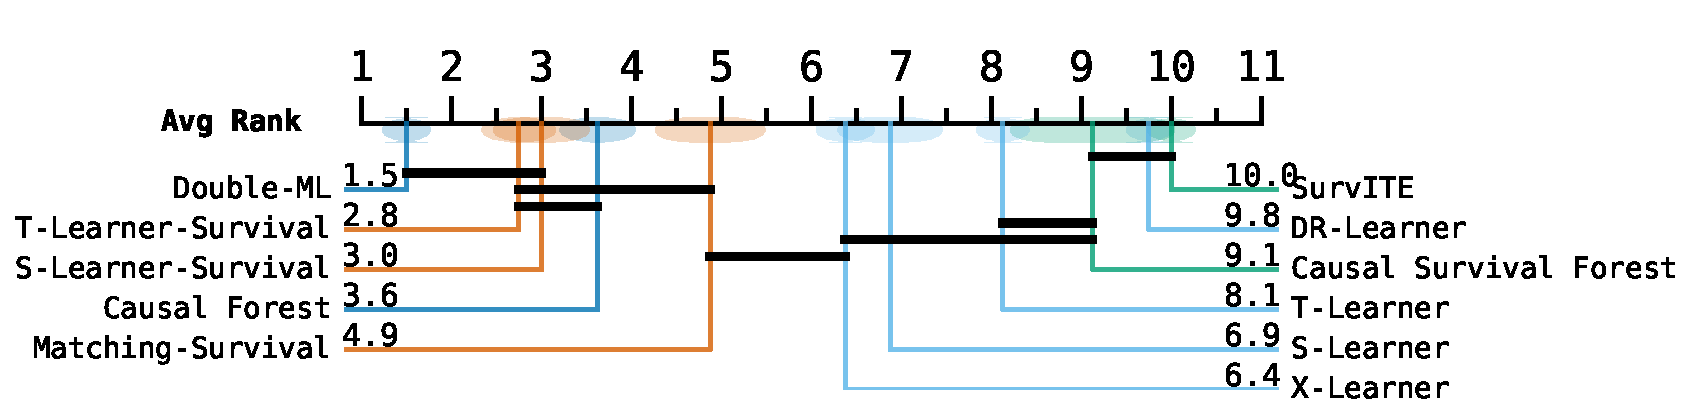
\includegraphics[width=\linewidth]{Appendices/appendix-ch04/images/figure_results_updated/average_ranks/average_ranking_visualization_method_combination_scenario_A.pdf}
        \centering
        
    \end{minipage}}
    \hfill
    \subfloat[{Scenario \texttt{B}}]{\begin{minipage}[t]{0.49\textwidth}
        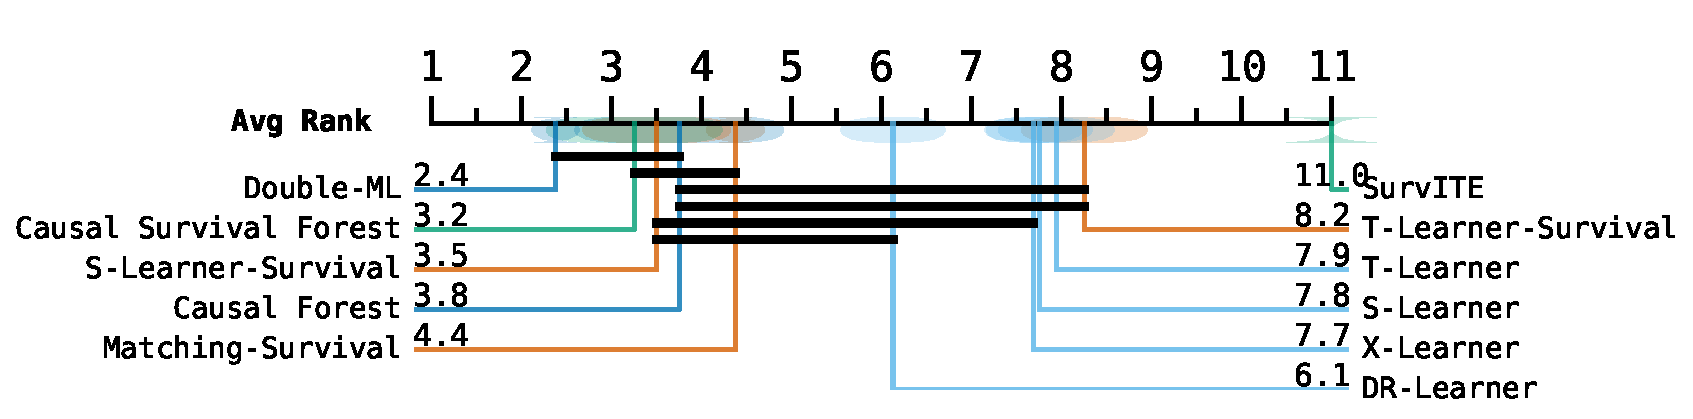
\includegraphics[width=\linewidth]{Appendices/appendix-ch04/images/figure_results_updated/average_ranks/average_ranking_visualization_method_combination_scenario_B.pdf}
        \centering
        
    \end{minipage}}

    

    \subfloat[{Scenario \texttt{C}}]{\begin{minipage}[t]{0.49\textwidth}
        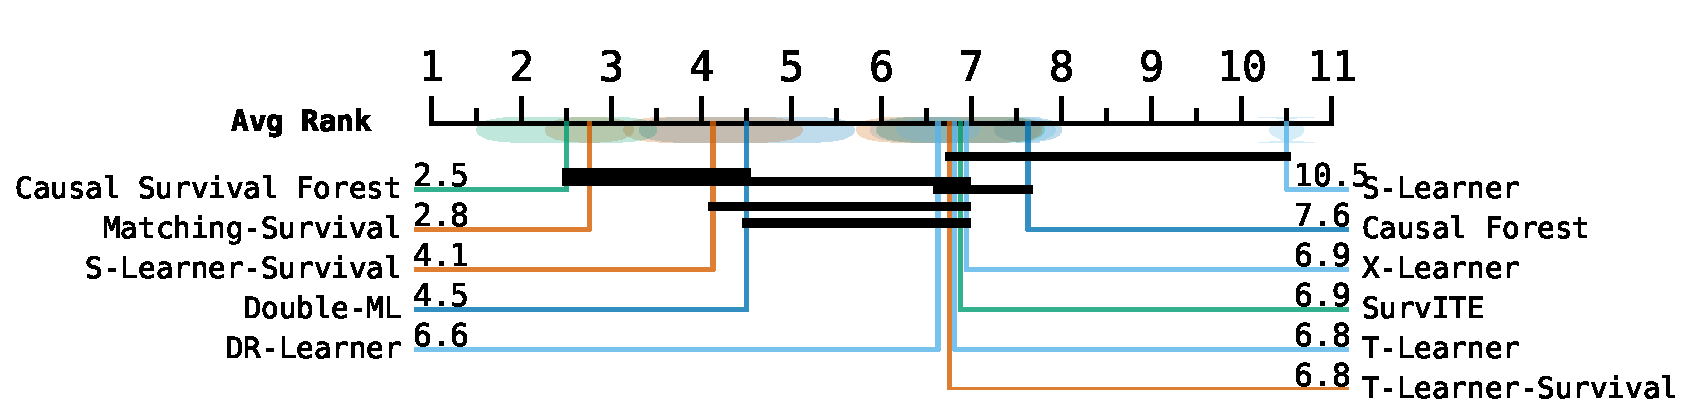
\includegraphics[width=\linewidth]{Appendices/appendix-ch04/images/figure_results_updated/average_ranks/average_ranking_visualization_method_combination_scenario_C.pdf}
        \centering
        
    \end{minipage}}
    \hfill
    \subfloat[{Scenario \texttt{D}}]{\begin{minipage}[t]{0.49\textwidth}
        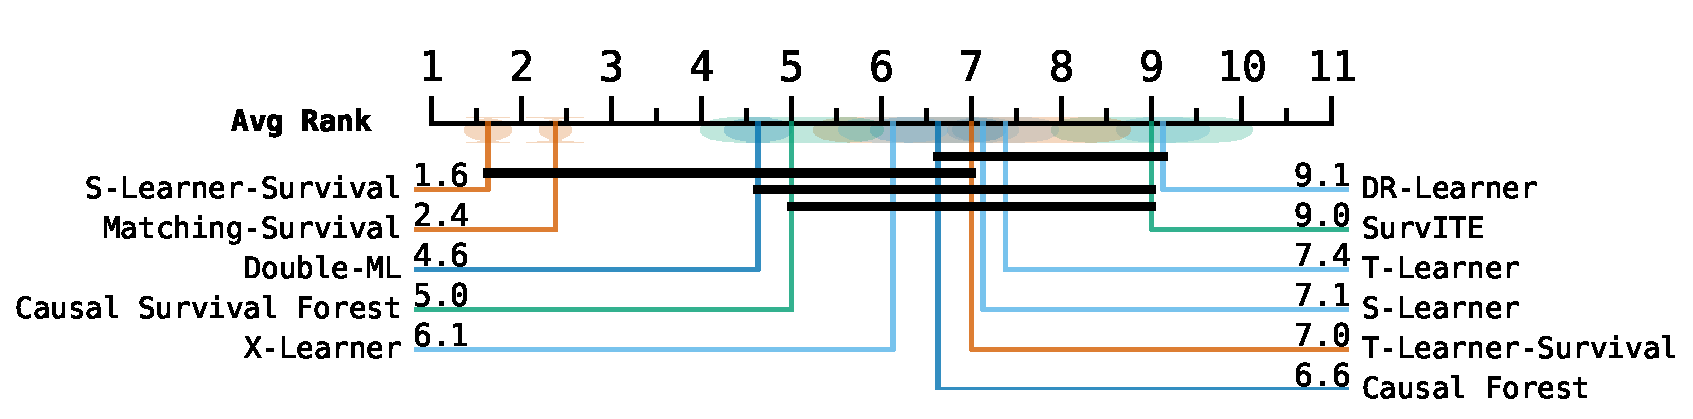
\includegraphics[width=\linewidth]{Appendices/appendix-ch04/images/figure_results_updated/average_ranks/average_ranking_visualization_method_combination_scenario_D.pdf}
        \centering
        
    \end{minipage}}

    

    \subfloat[{Scenario \texttt{E}}]{\begin{minipage}[t]{0.49\textwidth}
        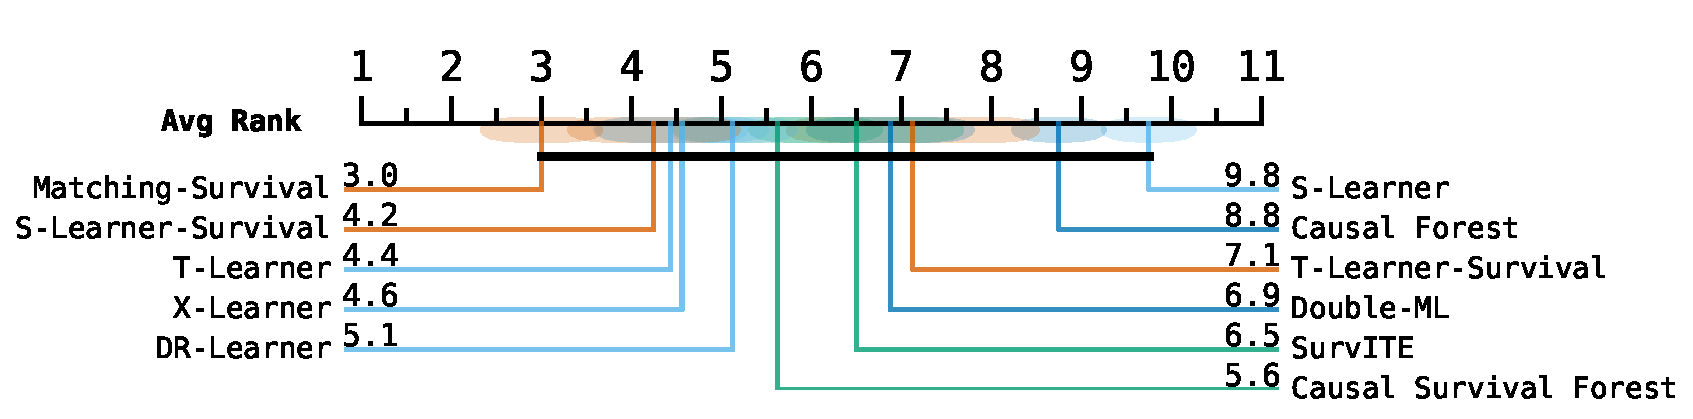
\includegraphics[width=\linewidth]{Appendices/appendix-ch04/images/figure_results_updated/average_ranks/average_ranking_visualization_method_combination_scenario_E.pdf}
        \centering
        
    \end{minipage}}

    \hfill

    
    
}
\end{figure}



% \ChFourRebuttal{In addition to the global rankings in Figure~\ref{ch04:fig:average_rank_per_scenario}, we report scenario-specific win-rates in Table~\ref{ch04:tab:scenario-winrates}. For each survival scenario (\texttt{A}--\texttt{E}), we compute how often each method family appears in the Top-1, Top-3, and Top-5 positions for CATE RMSE and \textcolor{black}{ATE Bias} across the eight causal configurations. This allows us to examine how the relative advantages of outcome imputation, direct-survival, and survival meta-learner approaches change as we vary both the survival time model (Cox, AFT, Poisson) and the censoring rate (low, medium, high; Table~\ref{ch04:tab:synthetic-data-survival-scenario}).}
\ChFourRebuttal{In addition to the global rankings in Figure~\ref{ch04:fig:average_rank_per_scenario}, we report scenario-specific win-rates in Table~\ref{ch04:tab:scenario-winrates}. For each survival scenario (\texttt{A}--\texttt{E}), we compute how often each method family appears in the Top-1, Top-3, and Top-5 positions for CATE RMSE and ATE Bias across the eight causal configurations. This provides a complementary view of robustness, highlighting which families consistently occupy the top ranks as we vary the survival time model (Cox, AFT, Poisson) and the censoring rate (low, medium, high; Table~\ref{ch04:tab:synthetic-data-survival-scenario}).}


% \ChFourRebuttal{Under low censoring (Scenarios~\texttt{A} and~\texttt{B}), outcome regression methods remain competitive, but their strengths are scenario-dependent. In Scenario~\texttt{A} (Cox, low censoring), Double-ML dominates CATE RMSE with a 100\% Top-1/Top-3/Top-5 win-rate, while Causal Forest is almost always in the Top-3 and Top-5. \textcolor{black}{ATE Bias is more dispersed}: SurvITE, DR-Learner, and several meta-learners share Top-1 and Top-3 positions, and Causal Survival Forests is frequently among the top methods. In Scenario~\texttt{B} (AFT, low censoring), Causal Survival Forests becomes the main winner, achieving the highest CATE RMSE win-rates (62.5\% Top-1 and 100\% Top-3/Top-5) and strong ATE Bias performance, with Double-ML and Causal Forest also appearing often in the Top-3 and Top-5.}
\ChFourRebuttal{Under low censoring (Scenarios~\texttt{A} and~\texttt{B}), outcome-imputation approaches can still be competitive on CATE RMSE, but the winners are scenario-dependent and survival-aware methods remain highly prevalent in the Top-$k$ sets. In Scenario~\texttt{A} (Cox, low censoring), Double-ML dominates CATE RMSE (62.5\% Top-1 and 100\% Top-3/Top-5), while survival meta-learners also appear frequently in Top-3/Top-5 (e.g., T-Learner-Survival and S-Learner-Survival are both 100\% Top-5). ATE Bias is more dispersed: S-Learner and DR-Learner each attain 25.0\% Top-1, and survival meta-learners (S-Learner-Survival and Matching-Survival) contribute strongly to Top-3/Top-5, whereas the direct-survival CATE methods have limited presence. In Scenario~\texttt{B} (AFT, low censoring), Causal Survival Forests becomes a leading family for both metrics (37.5\% Top-1 CATE RMSE; 25.0\% Top-1 ATE Bias; 75.0\% Top-3/Top-5 ATE Bias). At the same time, Causal Forest remains competitive on CATE RMSE (37.5\% Top-1), and survival meta-learners retain substantial Top-5 coverage, particularly Matching-Survival (87.5\% Top-5 CATE RMSE) and S-Learner-Survival (87.5\% Top-5 CATE RMSE). Notably, SurvITE does not appear among the Top-$k$ in this scenario.}

% \ChFourRebuttal{As censoring increases, survival-specific modeling becomes more important. In Scenario~\texttt{C} (Poisson, medium censoring), Causal Survival Forests clearly leads in both CATE RMSE and ATE Bias, with Double-ML and SurvITE providing additional support in the Top-3 and Top-5. Under high censoring (Scenarios~\texttt{D} and~\texttt{E}), the advantage of survival-focused methods is even more pronounced. In Scenario~\texttt{D} (AFT, high censoring), SurvITE and the survival meta-learners (S-Learner-Survival, Matching-Survival, and T-Learner-Survival) capture most Top-1 and Top-3 spots in CATE RMSE, while Causal Survival Forests and the same survival meta-learners dominate ATE Bias. In Scenario~\texttt{E} (Poisson, high censoring), Causal Survival Forests and the survival meta-learners again account for nearly all Top-1 and Top-3 positions for both metrics, with Double-ML mainly contributing through Top-5 appearances. Across these settings, classical meta-learners without survival structure rarely win, reinforcing that explicit survival modeling is crucial once censoring becomes moderate or high.}
\ChFourRebuttal{As censoring increases, survival-specific modeling becomes increasingly important and accounts for a larger fraction of the best-performing sets. In Scenario~\texttt{C} (Poisson, medium censoring), Causal Survival Forests clearly leads on both metrics (62.5\% Top-1 CATE RMSE; 37.5\% Top-1 ATE Bias; 100\% Top-5 ATE Bias), while Matching-Survival and S-Learner-Survival frequently appear among the best methods (e.g., Matching-Survival is 25.0\% Top-1 CATE RMSE and 100\% Top-5 CATE RMSE; both Matching-Survival and S-Learner-Survival reach 75.0\% Top-3 CATE RMSE). Under high censoring, the dominance shifts even more strongly toward survival-aware families, but with different emphases across scenarios. In Scenario~\texttt{D} (AFT, high censoring), S-Learner-Survival is the primary winner on CATE RMSE (50.0\% Top-1 and 100\% Top-3/Top-5), while Matching-Survival achieves perfect Top-3/Top-5 coverage (100\% in both cases). For ATE Bias, the top positions are shared across multiple survival-aware families (Causal Survival Forests, T-Learner-Survival, and S-Learner-Survival each at 25.0\% Top-1). In Scenario~\texttt{E} (Poisson, high censoring), the strongest ATE Bias performance is achieved by T-Learner-Survival (50.0\% Top-1 and 87.5\% Top-5), with Matching-Survival and SurvITE following, whereas CATE RMSE Top-1 is more distributed (Matching-Survival: 37.5\% Top-1; several other methods across both outcome-imputation and direct-survival CATE methods at 12.5\%). Overall, across all scenarios, classical outcome-imputation methods are rarely dominant or ranked Top-1 under moderate or high censoring, reinforcing the benefit of explicitly modeling time-to-event structure when the censoring rate is high.}


% !TeX root = ../../../main.tex
\begin{table}[htbp]
\ChFourFloatContents{ch04:tab:scenario-winrates}{\caption{\ChFourRebuttal{Win-rate (\%) of method families by Survival Scenario. 
Values denote the percentage of times a method appears in the Top-1, Top-3, and Top-5 
according to CATE RMSE and ATE Bias across the eight causal configurations for each scenario.}}}{
\centering



\begin{minipage}{0.48\textwidth}
\centering
\textbf{Scenario \texttt{A}: Cox, Low Censoring}\\[0.25em]
\begin{adjustbox}{max width=\textwidth}
\begin{tabular}{lccc@{\hspace{18pt}}ccc}
\toprule
\multirow{2}{*}{\textbf{Method Family}} &
\multicolumn{3}{c}{\textbf{CATE RMSE}} &
\multicolumn{3}{c}{\textbf{ATE Bias}} \\
\cmidrule(lr){2-4} \cmidrule(lr){5-7}
& \textbf{Top-1} & \textbf{Top-3} & \textbf{Top-5}
& \textbf{Top-1} & \textbf{Top-3} & \textbf{Top-5} \\
\midrule
\multicolumn{7}{l}{\textit{Outcome Imputation Methods}} \\
T-Learner               & \textcolor{gray}{0}   & \textcolor{gray}{0}   & \textcolor{gray}{0}   & \textcolor{gray}{0}   & 25.0 & 25.0 \\
S-Learner               & \textcolor{gray}{0}   & 12.5 & 12.5 & 25.0 & 50.0 & 50.0 \\
X-Learner               & \textcolor{gray}{0}   & \textcolor{gray}{0}   & 12.5 & \textcolor{gray}{0}   & 25.0 & 62.5 \\
DR-Learner              & \textcolor{gray}{0}   & \textcolor{gray}{0}   & \textcolor{gray}{0}   & 25.0 & 25.0 & 62.5 \\
Double-ML               & 62.5 & 100.0 & 100.0 & \textcolor{gray}{0}   & 12.5 & 37.5 \\
Causal Forest           & \textcolor{gray}{0}   & 37.5 & 100.0 & 12.5 & 12.5 & 37.5 \\
\addlinespace %
\multicolumn{7}{l}{\textit{Direct-Survival CATE Methods}} \\
Causal Survival Forests  & \textcolor{gray}{0}   & \textcolor{gray}{0}   & \textcolor{gray}{0}   & \textcolor{gray}{0}   & 12.5 & 25.0 \\
SurvITE                 & \textcolor{gray}{0}   & \textcolor{gray}{0}   & \textcolor{gray}{0}   & \textcolor{gray}{0}   & \textcolor{gray}{0}   & 25.0 \\
\addlinespace %
\multicolumn{7}{l}{\textit{Survival Meta-Learners}} \\
T-Learner-Survival      & 12.5 & 87.5 & 100.0 & 12.5 & 25.0 & 50.0 \\
S-Learner-Survival      & 25.0 & 50.0 & 100.0 & 12.5 & 62.5 & 75.0 \\
Matching-Survival       & \textcolor{gray}{0}   & 12.5 & 75.0 & 12.5 & 50.0 & 50.0 \\
\bottomrule
\end{tabular}
\end{adjustbox}
\end{minipage}
\hfill
\begin{minipage}{0.48\textwidth}
\centering
\textbf{Scenario \texttt{B}: AFT, Low Censoring}\\[0.25em]
\begin{adjustbox}{max width=\textwidth}
\begin{tabular}{lccc@{\hspace{18pt}}ccc}
\toprule
\multirow{2}{*}{\textbf{Method Family}} &
\multicolumn{3}{c}{\textbf{CATE RMSE}} &
\multicolumn{3}{c}{\textbf{ATE Bias}} \\
\cmidrule(lr){2-4} \cmidrule(lr){5-7}
& \textbf{Top-1} & \textbf{Top-3} & \textbf{Top-5}
& \textbf{Top-1} & \textbf{Top-3} & \textbf{Top-5} \\
\midrule
\multicolumn{7}{l}{\textit{Outcome Imputation Methods}} \\
T-Learner               & \textcolor{gray}{0}   & \textcolor{gray}{0}   & 12.5 & \textcolor{gray}{0}   & 12.5 & 25.0 \\
S-Learner               & \textcolor{gray}{0}   & \textcolor{gray}{0}   & \textcolor{gray}{0}   & \textcolor{gray}{0}   & 12.5 & 25.0 \\
X-Learner               & \textcolor{gray}{0}   & \textcolor{gray}{0}   & 12.5 & 12.5 & 12.5 & 37.5 \\
DR-Learner              & \textcolor{gray}{0}   & 12.5 & 25.0 & \textcolor{gray}{0}   & 25.0 & 37.5 \\
Double-ML               & 12.5 & 100.0 & 100.0 & 12.5 & 12.5 & 37.5 \\
Causal Forest           & 37.5 & 50.0 & 75.0 & \textcolor{gray}{0}   & 25.0 & 62.5 \\
\addlinespace %
\multicolumn{7}{l}{\textit{Direct-Survival CATE Methods}} \\
Causal Survival Forests  & 37.5 & 62.5 & 87.5 & 25.0 & 75.0 & 75.0 \\
SurvITE                 & \textcolor{gray}{0}   & \textcolor{gray}{0}   & \textcolor{gray}{0}   & \textcolor{gray}{0}   & \textcolor{gray}{0}   & \textcolor{gray}{0} \\
\addlinespace %
\multicolumn{7}{l}{\textit{Survival Meta-Learners}} \\
T-Learner-Survival      & \textcolor{gray}{0}   & \textcolor{gray}{0}   & 12.5 & 25.0 & 37.5 & 62.5 \\
S-Learner-Survival      & 12.5 & 62.5 & 87.5 & 12.5 & 37.5 & 62.5 \\
Matching-Survival       & \textcolor{gray}{0}   & 12.5 & 87.5 & 12.5 & 50.0 & 75.0 \\
\bottomrule
\end{tabular}
\end{adjustbox}
\end{minipage}



\begin{minipage}{0.48\textwidth}
\centering
\textbf{Scenario \texttt{C}: Poisson, Medium Censoring}\\[0.25em]
\begin{adjustbox}{max width=\textwidth}
\begin{tabular}{lccc@{\hspace{18pt}}ccc}
\toprule
\multirow{2}{*}{\textbf{Method Family}} &
\multicolumn{3}{c}{\textbf{CATE RMSE}} &
\multicolumn{3}{c}{\textbf{ATE Bias}} \\
\cmidrule(lr){2-4} \cmidrule(lr){5-7}
& \textbf{Top-1} & \textbf{Top-3} & \textbf{Top-5}
& \textbf{Top-1} & \textbf{Top-3} & \textbf{Top-5} \\
\midrule
\multicolumn{7}{l}{\textit{Outcome Imputation Methods}} \\
T-Learner               & \textcolor{gray}{0}   & 25.0 & 37.5 & \textcolor{gray}{0}   & 12.5 & 25.0 \\
S-Learner               & \textcolor{gray}{0}   & \textcolor{gray}{0}   & \textcolor{gray}{0}   & \textcolor{gray}{0}   & \textcolor{gray}{0}   & \textcolor{gray}{0} \\
X-Learner               & \textcolor{gray}{0}   & 25.0 & 37.5 & \textcolor{gray}{0}   & \textcolor{gray}{0}   & 25.0 \\
DR-Learner              & \textcolor{gray}{0}   & \textcolor{gray}{0}   & 25.0 & \textcolor{gray}{0}   & \textcolor{gray}{0}   & \textcolor{gray}{0} \\
Double-ML               & 12.5 & 50.0 & 62.5 & \textcolor{gray}{0}   & \textcolor{gray}{0}   & \textcolor{gray}{0} \\
Causal Forest           & \textcolor{gray}{0}   & \textcolor{gray}{0}   & \textcolor{gray}{0}   & \textcolor{gray}{0}   & \textcolor{gray}{0}   & \textcolor{gray}{0} \\
\addlinespace %
\multicolumn{7}{l}{\textit{Direct-Survival CATE Methods}} \\
Causal Survival Forests  & 62.5 & 75.0 & 87.5 & 37.5 & 75.0 & 100.0 \\
SurvITE                 & \textcolor{gray}{0}   & \textcolor{gray}{0}   & 50.0 & 25.0 & 50.0 & 87.5 \\
\addlinespace %
\multicolumn{7}{l}{\textit{Survival Meta-Learners}} \\
T-Learner-Survival      & \textcolor{gray}{0}   & 12.5 & 25.0 & 12.5 & 25.0 & 75.0 \\
S-Learner-Survival      & \textcolor{gray}{0}   & 62.5 & 75.0 & \textcolor{gray}{0}   & 62.5 & 100.0 \\
Matching-Survival       & 25.0 & 75.0 & 100.0 & 25.0 & 75.0 & 87.5 \\
\bottomrule
\end{tabular}
\end{adjustbox}
\end{minipage}
\hfill
\begin{minipage}{0.48\textwidth}
\centering
\textbf{Scenario \texttt{D}: AFT, High Censoring}\\[0.25em]
\begin{adjustbox}{max width=\textwidth}
\begin{tabular}{lccc@{\hspace{18pt}}ccc}
\toprule
\multirow{2}{*}{\textbf{Method Family}} &
\multicolumn{3}{c}{\textbf{CATE RMSE}} &
\multicolumn{3}{c}{\textbf{ATE Bias}} \\
\cmidrule(lr){2-4} \cmidrule(lr){5-7}
& \textbf{Top-1} & \textbf{Top-3} & \textbf{Top-5}
& \textbf{Top-1} & \textbf{Top-3} & \textbf{Top-5} \\
\midrule
\multicolumn{7}{l}{\textit{Outcome Imputation Methods}} \\
T-Learner               & \textcolor{gray}{0}   & \textcolor{gray}{0}   & 25.0 & 12.5 & 12.5 & 50.0 \\
S-Learner               & \textcolor{gray}{0}   & \textcolor{gray}{0}   & \textcolor{gray}{0}   & \textcolor{gray}{0}   & 12.5 & 50.0 \\
X-Learner               & \textcolor{gray}{0}   & \textcolor{gray}{0}   & 37.5 & 12.5 & 12.5 & 25.0 \\
DR-Learner              & \textcolor{gray}{0}   & \textcolor{gray}{0}   & \textcolor{gray}{0}   & \textcolor{gray}{0}   & 12.5 & 37.5 \\
Double-ML               & \textcolor{gray}{0}   & \textcolor{gray}{0}   & 87.5 & \textcolor{gray}{0}   & \textcolor{gray}{0}   & 12.5 \\
Causal Forest           & \textcolor{gray}{0}   & \textcolor{gray}{0}   & 37.5 & \textcolor{gray}{0}   & \textcolor{gray}{0}   & 37.5 \\
\addlinespace %
\multicolumn{7}{l}{\textit{Direct-Survival CATE Methods}} \\
Causal Survival Forests  & 12.5 & 50.0 & 50.0 & 25.0 & 62.5 & 87.5 \\
SurvITE                 & \textcolor{gray}{0}   & 12.5 & 25.0 & \textcolor{gray}{0}   & 12.5 & 12.5 \\
\addlinespace %
\multicolumn{7}{l}{\textit{Survival Meta-Learners}} \\
T-Learner-Survival      & 37.5 & 37.5 & 37.5 & 25.0 & 25.0 & 37.5 \\
S-Learner-Survival      & 50.0 & 100.0 & 100.0 & 25.0 & 75.0 & 75.0 \\
Matching-Survival       & \textcolor{gray}{0}   & 100.0 & 100.0 & 12.5 & 75.0 & 75.0 \\
\bottomrule
\end{tabular}
\end{adjustbox}
\end{minipage}



\begin{minipage}{0.48\textwidth}
\centering
\textbf{Scenario \texttt{E}: Poisson, High Censoring}\\[0.25em]
\begin{adjustbox}{max width=\textwidth}
\begin{tabular}{lccc@{\hspace{18pt}}ccc}
\toprule
\multirow{2}{*}{\textbf{Method Family}} &
\multicolumn{3}{c}{\textbf{CATE RMSE}} &
\multicolumn{3}{c}{\textbf{ATE Bias}} \\
\cmidrule(lr){2-4} \cmidrule(lr){5-7}
& \textbf{Top-1} & \textbf{Top-3} & \textbf{Top-5}
& \textbf{Top-1} & \textbf{Top-3} & \textbf{Top-5} \\
\midrule
\multicolumn{7}{l}{\textit{Outcome Imputation Methods}} \\
T-Learner               & 12.5 & 37.5 & 75.0 & \textcolor{gray}{0}   & 12.5 & 37.5 \\
S-Learner               & \textcolor{gray}{0}   & \textcolor{gray}{0}   & \textcolor{gray}{0}   & \textcolor{gray}{0}   & \textcolor{gray}{0}   & \textcolor{gray}{0} \\
X-Learner               & 12.5 & 37.5 & 75.0 & \textcolor{gray}{0}   & 37.5 & 50.0 \\
DR-Learner              & \textcolor{gray}{0}   & 25.0 & 62.5 & \textcolor{gray}{0}   & \textcolor{gray}{0}   & 12.5 \\
Double-ML               & 12.5 & 12.5 & 12.5 & \textcolor{gray}{0}   & \textcolor{gray}{0}   & \textcolor{gray}{0} \\
Causal Forest           & \textcolor{gray}{0}   & \textcolor{gray}{0}   & \textcolor{gray}{0}   & \textcolor{gray}{0}   & \textcolor{gray}{0}   & \textcolor{gray}{0} \\
\addlinespace %
\multicolumn{7}{l}{\textit{Direct-Survival CATE Methods}} \\
Causal Survival Forests  & 12.5 & 37.5 & 37.5 & \textcolor{gray}{0}   & 37.5 & 87.5 \\
SurvITE                 & 12.5 & 12.5 & 37.5 & 12.5 & 50.0 & 75.0 \\
\addlinespace %
\multicolumn{7}{l}{\textit{Survival Meta-Learners}} \\
T-Learner-Survival      & 12.5 & 25.0 & 37.5 & 50.0 & 75.0 & 87.5 \\
S-Learner-Survival      & \textcolor{gray}{0}   & 62.5 & 62.5 & 12.5 & 50.0 & 75.0 \\
Matching-Survival       & 37.5 & 50.0 & 100.0 & 25.0 & 37.5 & 75.0 \\
\bottomrule
\end{tabular}
\end{adjustbox}
\end{minipage}

}
\end{table}






%%%%%%%%%%%%%%%%%%%%%%%%%%%%%%%%%%%%%%%%%%%%%%%%%%%%%%%%%%%%
%%%%%%%%%%%%%%%%%%%%%%%%%%%%%%%%%%%%%%%%%%%%%%%%%%%%%%%%%%%%
%%%%%%%%%%%%%%%%%%%%%%%%%%%%%%%%%%%%%%%%%%%%%%%%%%%%%%%%%%%%

\subsubsection{Ranking of causal methods for different Causal Configurations}
\label{ch04:app:more-avg-rank}

% In Figure~\ref{ch04:fig:average_rank_per_experiments}, we present the Borda ranking of causal model families across eight distinct causal configurations, each representing different combinations of assumptions related to treatment assignment (RCT vs. observational), ignorability, positivity, and censoring mechanisms. Within each configuration, the average rank of each method is computed over all survival scenarios, allowing us to isolate how assumption violations affect model performance independently of survival data characteristics.
In Figure~\ref{ch04:fig:average_rank_per_experiments}, we present the Borda ranking of causal model families across eight distinct causal configurations, each representing different combinations of assumptions related to treatment assignment (RCT vs. observational), ignorability, positivity, and censoring mechanisms. Within each configuration, the average rank of each method is computed over all survival scenarios, allowing us to isolate how assumption violations affect model performance independently of survival data characteristics.
The colors of the lines connecting the methods to the horizontal axis represent the specific family of the method (e.g., outcome imputation based, direct-survival CATE, survival meta-learners).

% Notably, outcome imputation approaches such as X-Learner and Double-ML perform best in randomized settings with unbalanced treatment (e.g., RCT-5\%, panel b), but their performance deteriorates as we move to settings with unmeasured confounding, or more visibly with informative-censoring. In contrast, survival-specific methods such as S-Learner-Survival, Matching-Survival, and Causal Survival Forests consistently rise in the rankings under these challenging conditions--particularly when multiple violations occur simultaneously (e.g., panel g and h). This trend suggests that survival meta-learners and direct modeling of the survival process offer increased robustness to violations of standard causal assumptions, especially in the presence of unmeasured confounding and informative censoring. 
% Another finding here is that Causal Survival Forests maintains strong performance across many configurations, consistently ranking in the top half--particularly in settings involving unmeasured confounding or informative censoring. However, when the positivity assumption is violated (e.g., Figure~\ref{ch04:fig:average_rank_per_experiments}e and h), its performance declines, suggesting limitations in modeling highly sparse regions of the covariate space with deterministic treatment assignment.
Notably, outcome imputation approaches perform best in randomized settings with unbalanced treatment (e.g., RCT-5\%, Figure~\ref{ch04:fig:borda_ranking_causal_config_RCT_05}), where Double-ML achieves the top rank of 1.80.
However, their performance deteriorates as we move to settings with unmeasured confounding (Figure~\ref{ch04:fig:borda_ranking_causal_config_OBS_UConf}), or more visibly with informative censoring (Figures~\ref{ch04:fig:borda_ranking_causal_config_OBS_InfC},~\ref{ch04:fig:borda_ranking_causal_config_OBS_UConf_InfC},~\ref{ch04:fig:borda_ranking_causal_config_OBS_NoPos_InfC}), where Double-ML drops to the bottom of the top half and X-Learner falls entirely into the lower-performing half of the rankings.
In contrast, survival-specific methods of survival meta-learners such as S-Learner-Survival, Matching-Survival, and Causal Survival Forests (belonging to the direct-survival CATE family) consistently rise in the rankings under these conditions, particularly when multiple violations occur simultaneously (e.g., Figures~\ref{ch04:fig:borda_ranking_causal_config_OBS_UConf_InfC},~\ref{ch04:fig:borda_ranking_causal_config_OBS_NoPos_InfC}), where S-Learner-Survival and Matching-Survival take the top two spots.
This trend suggests that survival meta-learners and Causal Survival Forests, which directly model the survival process, offer increased robustness to violations of standard causal assumptions, especially in the presence of unmeasured confounding and informative censoring.
Another finding is that Causal Survival Forests maintains strong performance across many configurations, consistently ranking in the top half---particularly in settings involving informative censoring (e.g., Figures~\ref{ch04:fig:borda_ranking_causal_config_OBS_InfC},~\ref{ch04:fig:borda_ranking_causal_config_OBS_UConf_InfC}).
However, when the positivity assumption is violated while censoring remains ignorable (Figure~\ref{ch04:fig:borda_ranking_causal_config_OBS_NoPos}), its performance declines substantially, dropping to a rank of 6.60 in the bottom half of the ranking.
This suggests limitations in modeling highly sparse regions of the covariate space with deterministic treatment assignment under certain censoring conditions.


% !TeX root = ../../../main.tex
\begin{figure}[htbp]
\ChFourFloatContents{ch04:fig:average_rank_per_experiments}{\caption{Average ranking of each model for each causal configuration. \ChFourRebuttal{Shaded regions indicate the standard error of the rank across datasets.}}}{
    \centering

    \subfloat[{RCT: \ChFourGrayCheck (50\%), Ignorability: \ChFourGrayCheck, Positivity: \ChFourGrayCheck, Ign-Censoring: \ChFourGrayCheck}]{\begin{minipage}[t]{0.49\textwidth}
        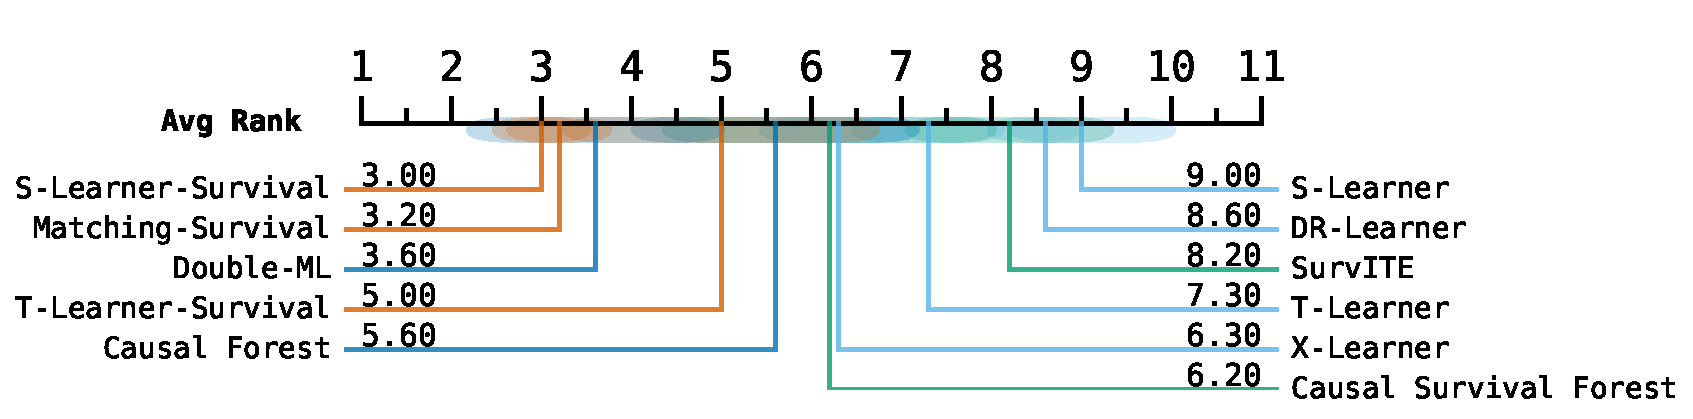
\includegraphics[width=\linewidth]{Appendices/appendix-ch04/images/figure_results_updated/average_ranks/average_ranking_visualization_method_combination_RCT-50.pdf}
        \centering
        
        \label{ch04:fig:borda_ranking_causal_config_RCT_50}
    \end{minipage}}
    \hfill
    \subfloat[{RCT: \ChFourGrayCheck (5\%), Ignorability: \ChFourGrayCheck, Positivity: \ChFourGrayCheck, Ign-Censoring: \ChFourGrayCheck}]{\begin{minipage}[t]{0.49\textwidth}
        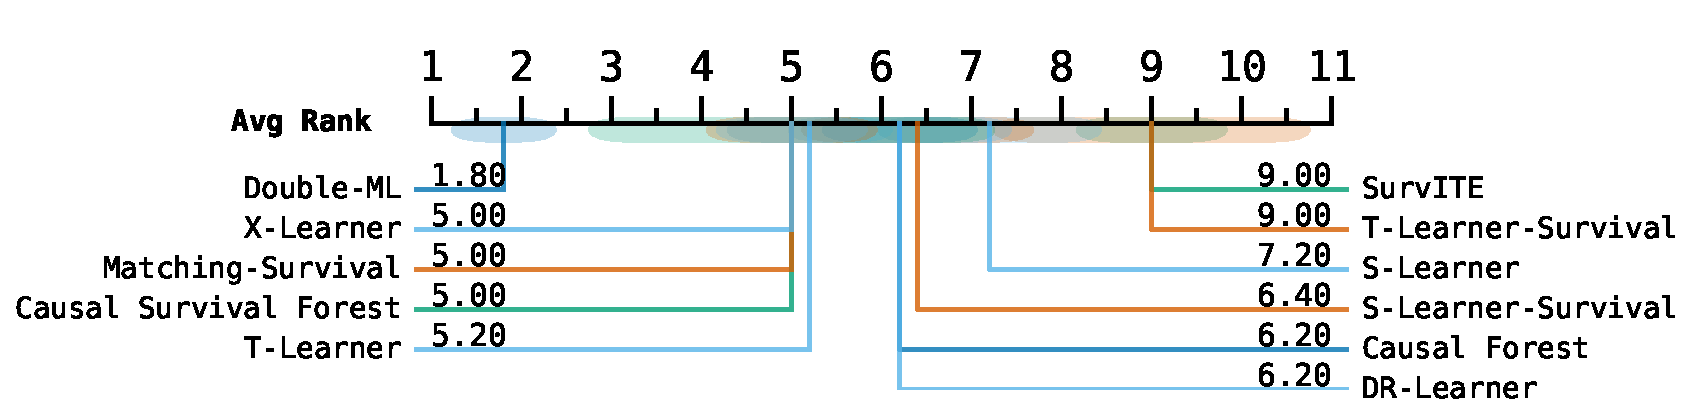
\includegraphics[width=\linewidth]{Appendices/appendix-ch04/images/figure_results_updated/average_ranks/average_ranking_visualization_method_combination_RCT-5.pdf}
        \centering
        
        \label{ch04:fig:borda_ranking_causal_config_RCT_05}
    \end{minipage}}

    

    \subfloat[{RCT: \ChFourBlackCross, Ignorability: \ChFourGrayCheck, Positivity: \ChFourGrayCheck, Ignorable Censoring: \ChFourGrayCheck}]{\begin{minipage}[t]{0.49\textwidth}
        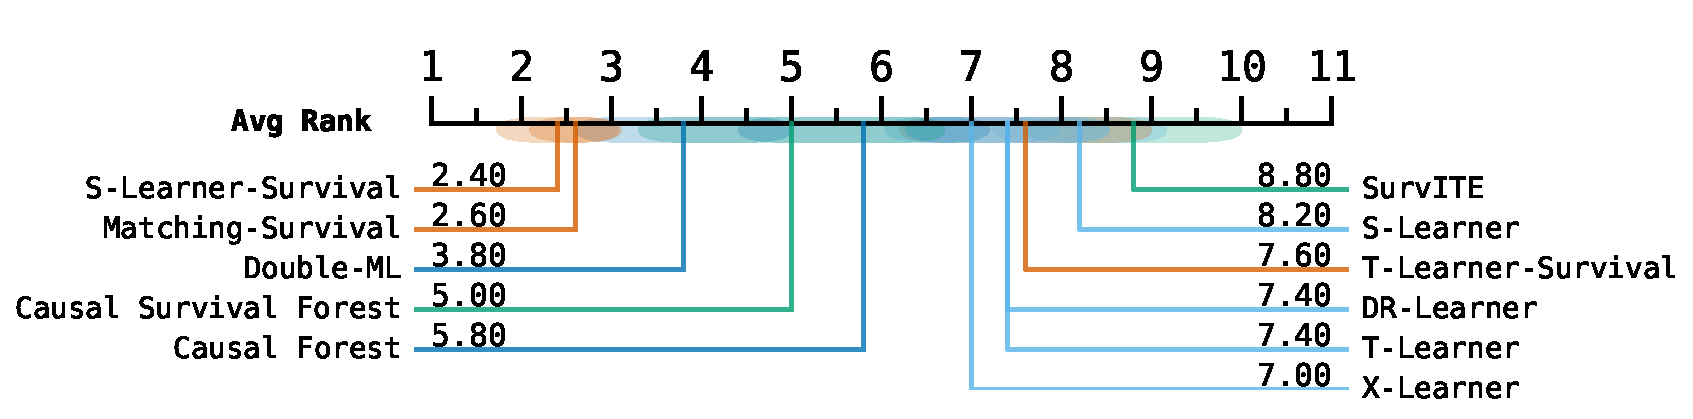
\includegraphics[width=\linewidth]{Appendices/appendix-ch04/images/figure_results_updated/average_ranks/average_ranking_visualization_method_combination_OBS-CPS.pdf}
        \centering
        
        \label{ch04:fig:borda_ranking_causal_config_OBS_CPS}
    \end{minipage}}
    \hfill
    \subfloat[{RCT: \ChFourBlackCross, Ignorability: \ChFourBlackCross, Positivity: \ChFourGrayCheck, Ignorable Censoring: \ChFourGrayCheck}]{\begin{minipage}[t]{0.49\textwidth}
        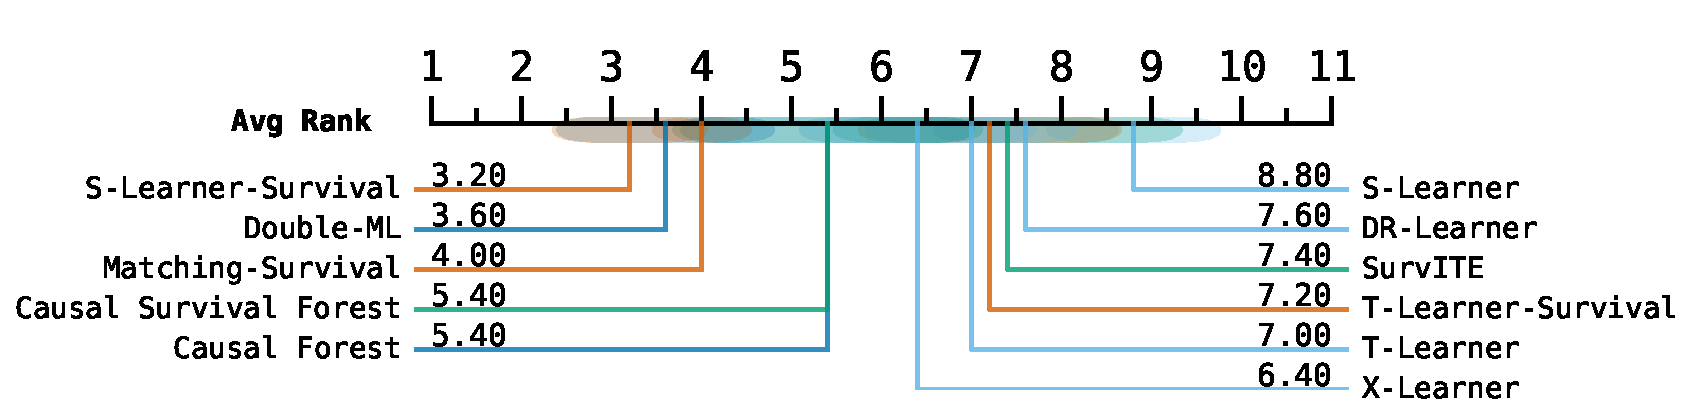
\includegraphics[width=\linewidth]{Appendices/appendix-ch04/images/figure_results_updated/average_ranks/average_ranking_visualization_method_combination_OBS-UConf.pdf}
        \centering
        
        \label{ch04:fig:borda_ranking_causal_config_OBS_UConf}
    \end{minipage}}

    

    \subfloat[{RCT: \ChFourBlackCross, Ignorability: \ChFourGrayCheck, Positivity: \ChFourBlackCross, Ignorable Censoring: \ChFourGrayCheck}]{\begin{minipage}[t]{0.49\textwidth}
        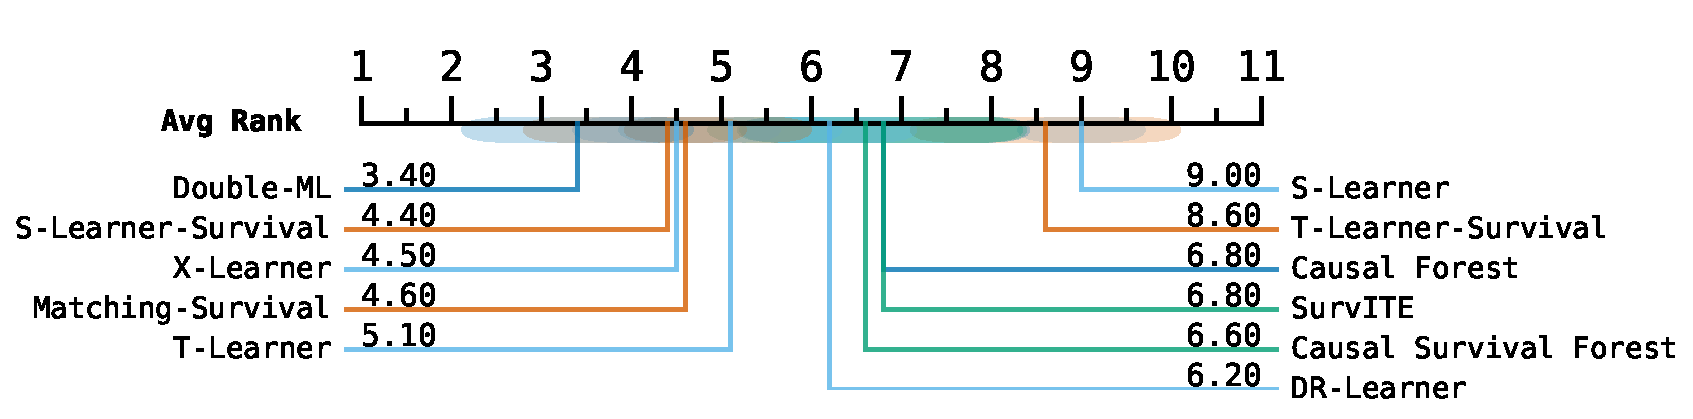
\includegraphics[width=\linewidth]{Appendices/appendix-ch04/images/figure_results_updated/average_ranks/average_ranking_visualization_method_combination_OBS-NoPos.pdf}
        \centering
        
        \label{ch04:fig:borda_ranking_causal_config_OBS_NoPos}
    \end{minipage}}
    \hfill
    \subfloat[{RCT: \ChFourBlackCross, Ignorability: \ChFourGrayCheck, Positivity: \ChFourGrayCheck, Ignorable Censoring: \ChFourBlackCross}]{\begin{minipage}[t]{0.49\textwidth}
        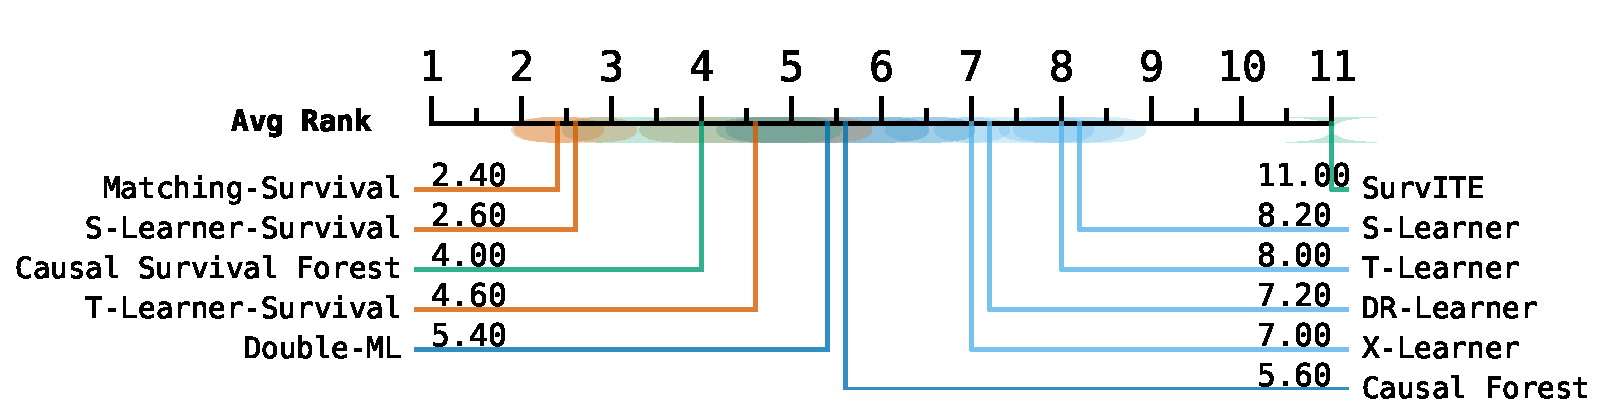
\includegraphics[width=\linewidth]{Appendices/appendix-ch04/images/figure_results_updated/average_ranks/average_ranking_visualization_method_combination_OBS-CPS-IC.pdf}
        \centering
        
        \label{ch04:fig:borda_ranking_causal_config_OBS_InfC}
    \end{minipage}}

    

    \subfloat[{RCT: \ChFourBlackCross, Ignorability: \ChFourBlackCross, Positivity: \ChFourGrayCheck, Ignorable Censoring: \ChFourBlackCross}]{\begin{minipage}[t]{0.49\textwidth}
        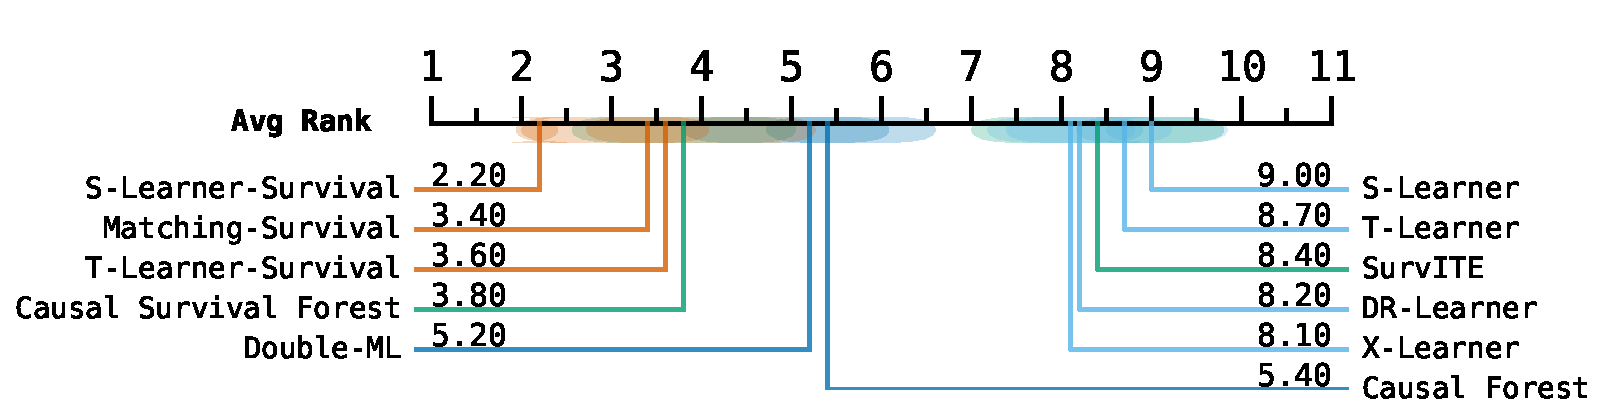
\includegraphics[width=\linewidth]{Appendices/appendix-ch04/images/figure_results_updated/average_ranks/average_ranking_visualization_method_combination_OBS-UConf-IC.pdf}
        \centering
        
        \label{ch04:fig:borda_ranking_causal_config_OBS_UConf_InfC}
    \end{minipage}}
    \hfill
    \subfloat[{RCT: \ChFourBlackCross, Ignorability: \ChFourGrayCheck, Positivity: \ChFourBlackCross, Ignorable Censoring: \ChFourBlackCross}]{\begin{minipage}[t]{0.49\textwidth}
        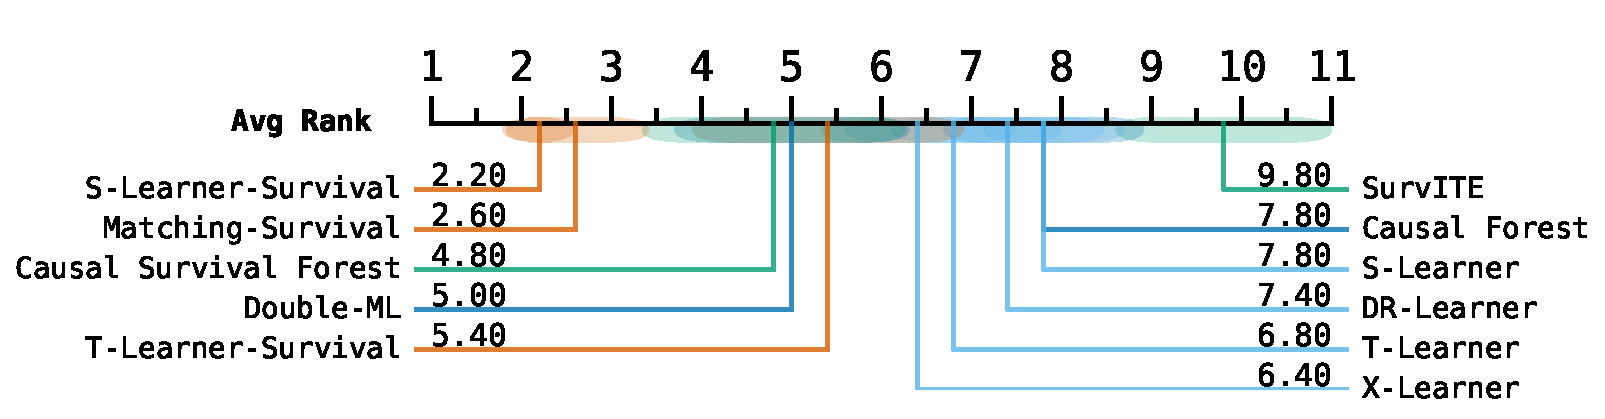
\includegraphics[width=\linewidth]{Appendices/appendix-ch04/images/figure_results_updated/average_ranks/average_ranking_visualization_method_combination_OBS-NoPos-IC.pdf}
        \centering
        
        \label{ch04:fig:borda_ranking_causal_config_OBS_NoPos_InfC}
    \end{minipage}}

    
    
}
\end{figure}



\ChFourRebuttal{In addition to the configuration-agnostic rankings in Figure~\ref{ch04:fig:average_rank_per_experiments}, we report win-rates by causal configuration in Tables~\ref{ch04:tab:winrate-rct-configs} and~\ref{ch04:tab:winrate-obs-configs}. For each configuration, we compute how often each method family appears in the Top-1, Top-3, and Top-5 positions for CATE RMSE and ATE Bias, aggregating over the five survival scenarios. This lets us separate the effect of causal assumptions (randomization, ignorability, positivity, and censoring) from the influence of the survival time model. The randomized settings (\texttt{RCT-50}, \texttt{RCT-5}) serve as our classical baselines, while the observational settings introduce unmeasured confounding, positivity violations, and informative censoring in a controlled way (Table~\ref{ch04:tab:synthetic-data-causal-config}).}

% \ChFourRebuttal{In the randomized configurations, outcome regression tends to perform well on CATE RMSE but is not uniformly dominant. Under \texttt{RCT-50}, Double-ML achieves the highest CATE RMSE win-rates (40.0 Top-1 and 80.0 Top-3/Top-5), with Causal Survival Forests and SurvITE also frequently appearing among the top methods. When treatment becomes sparse in \texttt{RCT-5}, Causal Survival Forests and Double-ML share the lead on CATE RMSE (Causal Survival Forests reaches 60.0 Top-1 and 80.0 Top-3/Top-5; Double-ML attains 20.0 Top-1 and 80.0 Top-5), while survival meta-learners such as S-Learner-Survival and Matching-Survival repeatedly enter the Top-3 and Top-5. Across both randomized settings, survival-specific approaches are already competitive on ATE Bias, with Causal Survival Forests, SurvITE, and several survival meta-learners appearing regularly among the top positions.}
\ChFourRebuttal{In the randomized configurations, CATE RMSE performance is split between outcome-imputation baselines and survival meta-learners, while ATE Bias results tend to favor survival-aware approaches. Under \texttt{RCT-50}, Double-ML, Causal Forest, Causal Survival Forests, T-Learner-Survival, and S-Learner-Survival all attain 20.0\% Top-1 on CATE RMSE, but the strongest Top-$k$ coverage comes from the survival meta-learners: S-Learner-Survival and Matching-Survival reach 100.0\% Top-5, and Matching-Survival achieves 60.0\% Top-3. For ATE Bias in \texttt{RCT-50}, S-Learner-Survival is the most frequent Top-1 method (40.0\%), with Causal Survival Forests and the survival meta-learners (including Matching-Survival and T-Learner-Survival) dominating Top-3/Top-5 (e.g., 60.0\% Top-3 for Causal Survival Forests and S-Learner-Survival; 80.0\% Top-5 for T-Learner-Survival, S-Learner-Survival, and Matching-Survival). When treatment assignment becomes sparse in \texttt{RCT-5}, Double-ML clearly leads on CATE RMSE (60.0\% Top-1 and 100.0\% Top-5), with Causal Survival Forests following (40.0\% Top-1; 60.0\% Top-3/Top-5). However, the ATE Bias rankings are largely driven by survival meta-learning: Matching-Survival achieves 40.0\% Top-1 and 80.0\% Top-3/Top-5, while S-Learner-Survival reaches 60.0\% Top-3/Top-5. Notably, SurvITE does not appear among the Top-$k$ in \texttt{RCT-5} and has only limited presence in \texttt{RCT-50}.}


% ============================
% RCT CONFIGURATIONS (GROUP 1)
% ============================

% !TeX root = ../../../main.tex
\begin{table}[htbp]
\ChFourFloatContents{ch04:tab:winrate-rct-configs}{\caption{\ChFourRebuttal{Win-rate (\%) of method families by Causal Configuration (randomized controlled trial settings). 
Values denote the percentage of times a method appears in the Top-1, Top-3, and Top-5 
according to CATE RMSE and ATE Bias across the five survival scenarios for each configuration.}}}{
\centering



\begin{minipage}{0.48\textwidth}
\centering
\textbf{\texttt{RCT-50}: 50\% treatment rate}\\[0.25em]
\begin{adjustbox}{max width=\textwidth}
\begin{tabular}{lccc@{\hspace{18pt}}ccc}
\toprule
\multirow{2}{*}{\textbf{Method Family}} &
\multicolumn{3}{c}{\textbf{CATE RMSE}} &
\multicolumn{3}{c}{\textbf{ATE Bias}} \\
\cmidrule(lr){2-4} \cmidrule(lr){5-7}
& \textbf{Top-1} & \textbf{Top-3} & \textbf{Top-5}
& \textbf{Top-1} & \textbf{Top-3} & \textbf{Top-5} \\
\midrule
\multicolumn{7}{l}{\textit{Outcome Imputation Methods}} \\
T-Learner               & \textcolor{gray}{0}   & \textcolor{gray}{0}   & 20.0 & \textcolor{gray}{0}   & 20.0 & 60.0 \\
S-Learner               & \textcolor{gray}{0}   & \textcolor{gray}{0}   & \textcolor{gray}{0}   & \textcolor{gray}{0}   & \textcolor{gray}{0}   & 20.0 \\
X-Learner               & \textcolor{gray}{0}   & \textcolor{gray}{0}   & 40.0 & 20.0 & 40.0 & 40.0 \\
DR-Learner              & \textcolor{gray}{0}   & \textcolor{gray}{0}   & \textcolor{gray}{0}   & \textcolor{gray}{0}   & 20.0 & 40.0 \\
Double-ML               & 20.0 & 60.0 & 80.0 & \textcolor{gray}{0}   & \textcolor{gray}{0}   & \textcolor{gray}{0} \\
Causal Forest           & 20.0 & 40.0 & 40.0 & \textcolor{gray}{0}   & \textcolor{gray}{0}   & 20.0 \\
\addlinespace %
\multicolumn{7}{l}{\textit{Direct-Survival CATE Methods}} \\
Causal Survival Forests  & 20.0 & 40.0 & 40.0 & 20.0 & 60.0 & 60.0 \\
SurvITE                 & \textcolor{gray}{0}   & \textcolor{gray}{0}   & 20.0 & \textcolor{gray}{0}   & 20.0 & 20.0 \\
\addlinespace %
\multicolumn{7}{l}{\textit{Survival Meta-Learners}} \\
T-Learner-Survival      & 20.0 & 40.0 & 60.0 & 20.0 & 40.0 & 80.0 \\
S-Learner-Survival      & 20.0 & 60.0 & 100.0 & 40.0 & 60.0 & 80.0 \\
Matching-Survival       & \textcolor{gray}{0}   & 60.0 & 100.0 & \textcolor{gray}{0}   & 40.0 & 80.0 \\
\bottomrule
\end{tabular}
\end{adjustbox}
\end{minipage}
\hfill
\begin{minipage}{0.48\textwidth}
\centering
\textbf{\texttt{RCT-5}: 5\% treatment rate}\\[0.25em]
\begin{adjustbox}{max width=\textwidth}
\begin{tabular}{lccc@{\hspace{18pt}}ccc}
\toprule
\multirow{2}{*}{\textbf{Method Family}} &
\multicolumn{3}{c}{\textbf{CATE RMSE}} &
\multicolumn{3}{c}{\textbf{ATE Bias}} \\
\cmidrule(lr){2-4} \cmidrule(lr){5-7}
& \textbf{Top-1} & \textbf{Top-3} & \textbf{Top-5}
& \textbf{Top-1} & \textbf{Top-3} & \textbf{Top-5} \\
\midrule
\multicolumn{7}{l}{\textit{Outcome Imputation Methods}} \\
T-Learner               & \textcolor{gray}{0}   & 20.0 & 60.0 & \textcolor{gray}{0}   & 20.0 & 60.0 \\
S-Learner               & \textcolor{gray}{0}   & 20.0 & 20.0 & 20.0 & 20.0 & 20.0 \\
X-Learner               & \textcolor{gray}{0}   & 20.0 & 60.0 & \textcolor{gray}{0}   & 20.0 & 60.0 \\
DR-Learner              & \textcolor{gray}{0}   & 20.0 & 40.0 & \textcolor{gray}{0}   & 20.0 & 60.0 \\
Double-ML               & 60.0 & 80.0 & 100.0 & 20.0 & 20.0 & 60.0 \\
Causal Forest           & \textcolor{gray}{0}   & \textcolor{gray}{0}   & 40.0 & \textcolor{gray}{0}   & 20.0 & 40.0 \\
\addlinespace %
\multicolumn{7}{l}{\textit{Direct-Survival CATE Methods}} \\
Causal Survival Forests  & 40.0 & 60.0 & 60.0 & 20.0 & 40.0 & 60.0 \\
SurvITE                 & \textcolor{gray}{0}   & \textcolor{gray}{0}   & \textcolor{gray}{0}   & \textcolor{gray}{0}   & \textcolor{gray}{0}   & \textcolor{gray}{0} \\
\addlinespace %
\multicolumn{7}{l}{\textit{Survival Meta-Learners}} \\
T-Learner-Survival      & \textcolor{gray}{0}   & 20.0 & 20.0 & \textcolor{gray}{0}   & \textcolor{gray}{0}   & \textcolor{gray}{0} \\
S-Learner-Survival      & \textcolor{gray}{0}   & 20.0 & 40.0 & \textcolor{gray}{0}   & 60.0 & 60.0 \\
Matching-Survival       & \textcolor{gray}{0}   & 40.0 & 60.0 & 40.0 & 80.0 & 80.0 \\
\bottomrule
\end{tabular}
\end{adjustbox}
\end{minipage}

}
\end{table}


% \ChFourRebuttal{The observational configurations highlight how violations of standard causal assumptions shift the balance further toward survival-focused methods. In \texttt{OBS-CPS} (no unmeasured confounding, no positivity or informative censoring), Double-ML and SurvITE are strong for CATE RMSE, but Causal Survival Forests and the survival meta-learners (especially S-Learner-Survival and Matching-Survival) capture most of the Top-1 and Top-3 spots for ATE Bias. Once unmeasured confounding is introduced (\texttt{OBS-UConf}), Causal Survival Forests, SurvITE, and the survival meta-learners dominate both metrics: Causal Survival Forests and Double-ML still perform well on CATE RMSE, but ATE Bias win-rates are almost entirely driven by Causal Survival Forests, SurvITE, S-Learner-Survival, and Matching-Survival. When positivity is violated (\texttt{OBS-NoPos}), Double-ML and SurvITE retain high CATE RMSE win-rates, whereas Causal Survival Forests and SurvITE achieve strong ATE Bias performance, and survival meta-learners again appear often in the Top-3 and Top-5.}
\ChFourRebuttal{The observational configurations further highlight how assumption violations shift performance toward survival-aware approaches, while revealing clear differences between \emph{direct-survival CATE} and \emph{survival meta-learner} families (Table~\ref{ch04:tab:winrate-obs-configs}). In \texttt{OBS-CPS} (no violations), CATE RMSE Top-1 is split across direct-survival CATE (Causal Survival Forests at 20.0\%) and Survival Meta-Learners (S-Learner-Survival and Matching-Survival at 20.0\% each), but the strongest Top-$k$ coverage comes from the Survival Meta-Learners: S-Learner-Survival and Matching-Survival reach 80.0\% Top-3 and 100.0\% Top-5. For ATE Bias in \texttt{OBS-CPS}, the lead is primarily driven by Survival Meta-Learners (S-Learner-Survival at 40.0\% Top-1; Matching-Survival at 80.0\% Top-3 and 100.0\% Top-5; T-Learner-Survival at 80.0\% Top-5), while the direct-survival CATE method Causal Survival Forests remains highly competitive in the upper ranks (60.0\% Top-3 and 80.0\% Top-5). Once unmeasured confounding is introduced (\texttt{OBS-UConf}), outcome imputation methods remain competitive for CATE RMSE (e.g., Double-ML at 20.0\% Top-1 and 80.0\% Top-5), but the top positions are shared with direct-survival CATE and Survival Meta-Learners (Causal Survival Forests, SurvITE, and S-Learner-Survival each at 20.0\% Top-1). For ATE Bias under \texttt{OBS-UConf}, direct-survival CATE takes the clearest lead at the very top (Causal Survival Forests at 40.0\% Top-1), while Survival Meta-Learners provide the strongest Top-3 presence (Matching-Survival at 60.0\% Top-3) and consistent Top-5 coverage (e.g., 60.0\% Top-5 for T-Learner-Survival, S-Learner-Survival, and Matching-Survival). Under positivity violations (\texttt{OBS-NoPos}), Outcome imputation dominates CATE RMSE Top-1 (Double-ML at 40.0\% and also T-Learner and X-Learner at 20.0\% each), whereas the Survival Meta-Learners remain highly competitive (S-Learner-Survival at 40.0\% Top-1 and 60.0\% Top-5; Matching-Survival at 80.0\% Top-5). In contrast, ATE Bias in \texttt{OBS-NoPos} is driven mainly by direct-survival CATE and Survival Meta-Learners: Causal Survival Forests reaches 80.0\% Top-3/Top-5, while Matching-Survival attains 40.0\% Top-1 coverage.}


% \ChFourRebuttal{Informative censoring amplifies these trends. In \texttt{OBS-CPS-InfC}, Causal Survival Forests, S-Learner-Survival, and Matching-Survival account for most of the Top-1 and Top-3 appearances for both CATE RMSE and ATE Bias, while Double-ML is mostly confined to Top-5 ranks. Under \texttt{OBS-UConf-InfC}, Causal Survival Forests becomes overwhelmingly dominant, reaching 80.0 Top-1 and 100.0 Top-3/Top-5 for CATE RMSE and similarly high win-rates for ATE Bias, with survival meta-learners providing additional support. Finally, in \texttt{OBS-NoPos-InfC}, Double-ML and Causal Survival Forests still perform well on CATE RMSE, but ATE Bias is largely controlled by Causal Survival Forests and the survival meta-learners, particularly T-Learner-Survival, S-Learner-Survival, and Matching-Survival. Overall, these patterns reinforce that direct survival modeling and survival meta-learning offer robustness as assumptions are progressively violated, especially when unmeasured confounding and informative censoring are present.}
\ChFourRebuttal{Informative censoring amplifies these differences and further separates the three method families. In \texttt{OBS-CPS-InfC}, CATE RMSE Top-1 is led by the direct-survival CATE family via Causal Survival Forests (40.0\%), while Survival Meta-Learners dominate Top-3/Top-5 coverage (S-Learner-Survival and Matching-Survival at 80.0\% Top-3 and 100.0\% Top-5). For ATE Bias in \texttt{OBS-CPS-InfC}, Survival Meta-Learners are the clear winners in the upper ranks (S-Learner-Survival at 100.0\% Top-3/Top-5; T-Learner-Survival at 40.0\% Top-1 and 80.0\% Top-5), with direct-survival CATE (Causal Survival Forests) still frequently among the top methods (80.0\% Top-5). Under \texttt{OBS-UConf-InfC}, CATE RMSE Top-1 is shared by direct-survival CATE (Causal Survival Forests at 40.0\%) and Survival Meta-Learners (T-Learner-Survival at 40.0\%), while Survival Meta-Learners dominate Top-3/Top-5 (S-Learner-Survival at 100.0\% Top-3/Top-5; Matching-Survival at 100.0\% Top-5). For ATE Bias in \texttt{OBS-UConf-InfC}, the strongest Top-1 signal comes from Survival Meta-Learners (T-Learner-Survival at 40.0\%), while direct-survival CATE shows the most dominant Top-5 presence (Causal Survival Forests at 100.0\% Top-5). Finally, in \texttt{OBS-NoPos-InfC}, Survival Meta-Learners clearly lead CATE RMSE (Matching-Survival at 40.0\% Top-1 and 100.0\% Top-5; S-Learner-Survival at 100.0\% Top-3/Top-5), whereas ATE Bias is again primarily driven by Survival Meta-Learners (T-Learner-Survival at 60.0\% Top-1 and 100.0\% Top-5), with direct-survival CATE remaining highly competitive in the upper ranks (Causal Survival Forests at 60.0\% Top-3 and 80.0\% Top-5). Overall, these patterns reinforce that as assumptions are progressively violated, Outcome imputation families can remain competitive for CATE RMSE in some regimes (notably \texttt{OBS-NoPos}), but direct-survival CATE and Survival Meta-Learners dominate the upper ranks for ATE Bias, especially under informative censoring and in settings with multiple simultaneous violations.}

% ================================
% OBSERVATIONAL CONFIGS (GROUP 2)
% ================================

% !TeX root = ../../../main.tex
\begin{table}[htbp]
\ChFourFloatContents{ch04:tab:winrate-obs-configs}{\caption{\ChFourRebuttal{Win-rate (\%) of method families by Causal Configuration (observational study settings). 
Values denote the percentage of times a method appears in the Top-1, Top-3, and Top-5 according to CATE RMSE and ATE Bias across the five survival scenarios for each configuration. }}}{
\centering



\begin{minipage}{0.48\textwidth}
\centering
\textbf{\texttt{OBS-CPS}}\\[0.25em]
\begin{adjustbox}{max width=\textwidth}
\begin{tabular}{lccc@{\hspace{18pt}}ccc}
\toprule
\multirow{2}{*}{\textbf{Method Family}} &
\multicolumn{3}{c}{\textbf{CATE RMSE}} &
\multicolumn{3}{c}{\textbf{ATE Bias}} \\
\cmidrule(lr){2-4} \cmidrule(lr){5-7}
& \textbf{Top-1} & \textbf{Top-3} & \textbf{Top-5}
& \textbf{Top-1} & \textbf{Top-3} & \textbf{Top-5} \\
\midrule
\multicolumn{7}{l}{\textit{Outcome Imputation Methods}} \\
T-Learner               & \textcolor{gray}{0}   & \textcolor{gray}{0}   & 40.0 & \textcolor{gray}{0}   & \textcolor{gray}{0}   & 20.0 \\
S-Learner               & \textcolor{gray}{0}   & \textcolor{gray}{0}   & \textcolor{gray}{0}   & \textcolor{gray}{0}   & \textcolor{gray}{0}   & 20.0 \\
X-Learner               & \textcolor{gray}{0}   & \textcolor{gray}{0}   & 20.0 & \textcolor{gray}{0}   & 20.0 & 20.0 \\
DR-Learner              & \textcolor{gray}{0}   & 20.0 & 20.0 & \textcolor{gray}{0}   & \textcolor{gray}{0}   & \textcolor{gray}{0} \\
Double-ML               & 20.0 & 40.0 & 80.0 & \textcolor{gray}{0}   & \textcolor{gray}{0}   & \textcolor{gray}{0} \\
Causal Forest           & 20.0 & 20.0 & 40.0 & \textcolor{gray}{0}   & 20.0 & 20.0 \\
\addlinespace %
\multicolumn{7}{l}{\textit{Direct-Survival CATE Methods}} \\
Causal Survival Forests  & 20.0 & 40.0 & 60.0 & \textcolor{gray}{0}   & 60.0 & 80.0 \\
SurvITE                 & \textcolor{gray}{0}   & \textcolor{gray}{0}   & 20.0 & 20.0 & 20.0 & 60.0 \\
\addlinespace %
\multicolumn{7}{l}{\textit{Survival Meta-Learners}} \\
T-Learner-Survival      & \textcolor{gray}{0}   & 20.0 & 20.0 & 20.0 & 40.0 & 80.0 \\
S-Learner-Survival      & 20.0 & 80.0 & 100.0 & 40.0 & 60.0 & 100.0 \\
Matching-Survival       & 20.0 & 80.0 & 100.0 & 20.0 & 80.0 & 100.0 \\
\bottomrule
\end{tabular}
\end{adjustbox}
\end{minipage}
\hfill
\begin{minipage}{0.48\textwidth}
\centering
\textbf{\texttt{OBS-UConf}}\\[0.25em]
\begin{adjustbox}{max width=\textwidth}
\begin{tabular}{lccc@{\hspace{18pt}}ccc}
\toprule
\multirow{2}{*}{\textbf{Method Family}} &
\multicolumn{3}{c}{\textbf{CATE RMSE}} &
\multicolumn{3}{c}{\textbf{ATE Bias}} \\
\cmidrule(lr){2-4} \cmidrule(lr){5-7}
& \textbf{Top-1} & \textbf{Top-3} & \textbf{Top-5}
& \textbf{Top-1} & \textbf{Top-3} & \textbf{Top-5} \\
\midrule
\multicolumn{7}{l}{\textit{Outcome Imputation Methods}} \\
T-Learner               & \textcolor{gray}{0}   & 20.0 & 20.0 & \textcolor{gray}{0}   & 20.0 & 40.0 \\
S-Learner               & \textcolor{gray}{0}   & \textcolor{gray}{0}   & \textcolor{gray}{0}   & \textcolor{gray}{0}   & 40.0 & 40.0 \\
X-Learner               & \textcolor{gray}{0}   & 20.0 & 40.0 & \textcolor{gray}{0}   & \textcolor{gray}{0}   & 60.0 \\
DR-Learner              & \textcolor{gray}{0}   & \textcolor{gray}{0}   & 20.0 & 20.0 & 40.0 & 40.0 \\
Double-ML               & 20.0 & 60.0 & 80.0 & \textcolor{gray}{0}   & \textcolor{gray}{0}   & 20.0 \\
Causal Forest           & 20.0 & 40.0 & 40.0 & \textcolor{gray}{0}   & \textcolor{gray}{0}   & 20.0 \\
\addlinespace %
\multicolumn{7}{l}{\textit{Direct-Survival CATE Methods}} \\
Causal Survival Forests  & 20.0 & 40.0 & 60.0 & 40.0 & 60.0 & 60.0 \\
SurvITE                 & 20.0 & 20.0 & 40.0 & 20.0 & 40.0 & 40.0 \\
\addlinespace %
\multicolumn{7}{l}{\textit{Survival Meta-Learners}} \\
T-Learner-Survival      & \textcolor{gray}{0}   & 20.0 & 20.0 & \textcolor{gray}{0}   & \textcolor{gray}{0}   & 60.0 \\
S-Learner-Survival      & 20.0 & 60.0 & 80.0 & \textcolor{gray}{0}   & 40.0 & 60.0 \\
Matching-Survival       & \textcolor{gray}{0}   & 20.0 & 100.0 & 20.0 & 60.0 & 60.0 \\
\bottomrule
\end{tabular}
\end{adjustbox}
\end{minipage}



\begin{minipage}{0.48\textwidth}
\centering
\textbf{\texttt{OBS-NoPos}}\\[0.25em]
\begin{adjustbox}{max width=\textwidth}
\begin{tabular}{lccc@{\hspace{18pt}}ccc}
\toprule
\multirow{2}{*}{\textbf{Method Family}} &
\multicolumn{3}{c}{\textbf{CATE RMSE}} &
\multicolumn{3}{c}{\textbf{ATE Bias}} \\
\cmidrule(lr){2-4} \cmidrule(lr){5-7}
& \textbf{Top-1} & \textbf{Top-3} & \textbf{Top-5}
& \textbf{Top-1} & \textbf{Top-3} & \textbf{Top-5} \\
\midrule
\multicolumn{7}{l}{\textit{Outcome Imputation Methods}} \\
T-Learner               & 20.0 & 40.0 & 60.0 & \textcolor{gray}{0}   & 20.0 & 40.0 \\
S-Learner               & \textcolor{gray}{0}   & \textcolor{gray}{0}   & \textcolor{gray}{0}   & \textcolor{gray}{0}   & 40.0 & 60.0 \\
X-Learner               & 20.0 & 40.0 & 80.0 & \textcolor{gray}{0}   & 20.0 & 60.0 \\
DR-Learner              & \textcolor{gray}{0}   & 20.0 & 20.0 & \textcolor{gray}{0}   & \textcolor{gray}{0}   & 40.0 \\
Double-ML               & 40.0 & 60.0 & 60.0 & \textcolor{gray}{0}   & 20.0 & 20.0 \\
Causal Forest           & \textcolor{gray}{0}   & 20.0 & 40.0 & 20.0 & 20.0 & 20.0 \\
\addlinespace %
\multicolumn{7}{l}{\textit{Direct-Survival CATE Methods}} \\
Causal Survival Forests  & \textcolor{gray}{0}   & 40.0 & 40.0 & 20.0 & 80.0 & 80.0 \\
SurvITE                 & \textcolor{gray}{0}   & 20.0 & 40.0 & \textcolor{gray}{0}   & 20.0 & 40.0 \\
\addlinespace %
\multicolumn{7}{l}{\textit{Survival Meta-Learners}} \\
T-Learner-Survival      & \textcolor{gray}{0}   & 20.0 & 20.0 & 20.0 & 20.0 & 20.0 \\
S-Learner-Survival      & 40.0 & 40.0 & 60.0 & \textcolor{gray}{0}   & 20.0 & 80.0 \\
Matching-Survival       & \textcolor{gray}{0}   & 20.0 & 80.0 & 40.0 & 40.0 & 40.0 \\
\bottomrule
\end{tabular}
\end{adjustbox}
\end{minipage}
\hfill
\begin{minipage}{0.48\textwidth}
\centering
\textbf{\texttt{OBS-CPS-InfC}}\\[0.25em]
\begin{adjustbox}{max width=\textwidth}
\begin{tabular}{lccc@{\hspace{18pt}}ccc}
\toprule
\multirow{2}{*}{\textbf{Method Family}} &
\multicolumn{3}{c}{\textbf{CATE RMSE}} &
\multicolumn{3}{c}{\textbf{ATE Bias}} \\
\cmidrule(lr){2-4} \cmidrule(lr){5-7}
& \textbf{Top-1} & \textbf{Top-3} & \textbf{Top-5}
& \textbf{Top-1} & \textbf{Top-3} & \textbf{Top-5} \\
\midrule
\multicolumn{7}{l}{\textit{Outcome Imputation Methods}} \\
T-Learner               & \textcolor{gray}{0}   & \textcolor{gray}{0}   & \textcolor{gray}{0}   & \textcolor{gray}{0}   & \textcolor{gray}{0}   & \textcolor{gray}{0} \\
S-Learner               & \textcolor{gray}{0}   & \textcolor{gray}{0}   & \textcolor{gray}{0}   & \textcolor{gray}{0}   & \textcolor{gray}{0}   & \textcolor{gray}{0} \\
X-Learner               & \textcolor{gray}{0}   & \textcolor{gray}{0}   & \textcolor{gray}{0}   & \textcolor{gray}{0}   & \textcolor{gray}{0}   & 40.0 \\
DR-Learner              & \textcolor{gray}{0}   & \textcolor{gray}{0}   & 40.0 & 20.0 & 20.0 & 20.0 \\
Double-ML               & \textcolor{gray}{0}   & 40.0 & 60.0 & \textcolor{gray}{0}   & \textcolor{gray}{0}   & \textcolor{gray}{0} \\
Causal Forest           & \textcolor{gray}{0}   & 20.0 & 60.0 & \textcolor{gray}{0}   & \textcolor{gray}{0}   & 40.0 \\
\addlinespace %
\multicolumn{7}{l}{\textit{Direct-Survival CATE Methods}} \\
Causal Survival Forests  & 40.0 & 60.0 & 60.0 & 20.0 & 40.0 & 80.0 \\
SurvITE                 & \textcolor{gray}{0}   & \textcolor{gray}{0}   & \textcolor{gray}{0}   & 20.0 & 20.0 & 60.0 \\
\addlinespace %
\multicolumn{7}{l}{\textit{Survival Meta-Learners}} \\
T-Learner-Survival      & 20.0 & 20.0 & 80.0 & 40.0 & 60.0 & 80.0 \\
S-Learner-Survival      & 20.0 & 80.0 & 100.0 & \textcolor{gray}{0}   & 100.0 & 100.0 \\
Matching-Survival       & 20.0 & 80.0 & 100.0 & \textcolor{gray}{0}   & 60.0 & 80.0 \\
\bottomrule
\end{tabular}
\end{adjustbox}
\end{minipage}



\begin{minipage}{0.48\textwidth}
\centering
\textbf{\texttt{OBS-UConf-InfC}}\\[0.25em]
\begin{adjustbox}{max width=\textwidth}
\begin{tabular}{lccc@{\hspace{18pt}}ccc}
\toprule
\multirow{2}{*}{\textbf{Method Family}} &
\multicolumn{3}{c}{\textbf{CATE RMSE}} &
\multicolumn{3}{c}{\textbf{ATE Bias}} \\
\cmidrule(lr){2-4} \cmidrule(lr){5-7}
& \textbf{Top-1} & \textbf{Top-3} & \textbf{Top-5}
& \textbf{Top-1} & \textbf{Top-3} & \textbf{Top-5} \\
\midrule
\multicolumn{7}{l}{\textit{Outcome Imputation Methods}} \\
T-Learner               & \textcolor{gray}{0}   & \textcolor{gray}{0}   & \textcolor{gray}{0}   & \textcolor{gray}{0}   & 20.0 & 20.0 \\
S-Learner               & \textcolor{gray}{0}   & \textcolor{gray}{0}   & \textcolor{gray}{0}   & 20.0 & 20.0 & 20.0 \\
X-Learner               & \textcolor{gray}{0}   & \textcolor{gray}{0}   & \textcolor{gray}{0}   & \textcolor{gray}{0}   & 20.0 & 20.0 \\
DR-Learner              & \textcolor{gray}{0}   & \textcolor{gray}{0}   & \textcolor{gray}{0}   & \textcolor{gray}{0}   & \textcolor{gray}{0}   & 20.0 \\
Double-ML               & \textcolor{gray}{0}   & 40.0 & 60.0 & \textcolor{gray}{0}   & \textcolor{gray}{0}   & 20.0 \\
Causal Forest           & \textcolor{gray}{0}   & \textcolor{gray}{0}   & 60.0 & \textcolor{gray}{0}   & \textcolor{gray}{0}   & 20.0 \\
\addlinespace %
\multicolumn{7}{l}{\textit{Direct-Survival CATE Methods}} \\
Causal Survival Forests  & 40.0 & 40.0 & 60.0 & \textcolor{gray}{0}   & 20.0 & 100.0 \\
SurvITE                 & \textcolor{gray}{0}   & \textcolor{gray}{0}   & 40.0 & \textcolor{gray}{0}   & 20.0 & 40.0 \\
\addlinespace %
\multicolumn{7}{l}{\textit{Survival Meta-Learners}} \\
T-Learner-Survival      & 40.0 & 80.0 & 80.0 & 40.0 & 60.0 & 80.0 \\
S-Learner-Survival      & \textcolor{gray}{0}   & 100.0 & 100.0 & 20.0 & 80.0 & 80.0 \\
Matching-Survival       & 20.0 & 40.0 & 100.0 & 20.0 & 60.0 & 80.0 \\
\bottomrule
\end{tabular}
\end{adjustbox}
\end{minipage}
\hfill
\begin{minipage}{0.48\textwidth}
\centering
\textbf{\texttt{OBS-NoPos-InfC}}\\[0.25em]
\begin{adjustbox}{max width=\textwidth}
\begin{tabular}{lccc@{\hspace{18pt}}ccc}
\toprule
\multirow{2}{*}{\textbf{Method Family}} &
\multicolumn{3}{c}{\textbf{CATE RMSE}} &
\multicolumn{3}{c}{\textbf{ATE Bias}} \\
\cmidrule(lr){2-4} \cmidrule(lr){5-7}
& \textbf{Top-1} & \textbf{Top-3} & \textbf{Top-5}
& \textbf{Top-1} & \textbf{Top-3} & \textbf{Top-5} \\
\midrule
\multicolumn{7}{l}{\textit{Outcome Imputation Methods}} \\
T-Learner               & \textcolor{gray}{0}   & 20.0 & 40.0 & 20.0 & 20.0 & 20.0 \\
S-Learner               & \textcolor{gray}{0}   & \textcolor{gray}{0}   & \textcolor{gray}{0}   & \textcolor{gray}{0}   & \textcolor{gray}{0}   & 20.0 \\
X-Learner               & \textcolor{gray}{0}   & 20.0 & 40.0 & 20.0 & 20.0 & 20.0 \\
DR-Learner              & \textcolor{gray}{0}   & \textcolor{gray}{0}   & 40.0 & \textcolor{gray}{0}   & \textcolor{gray}{0}   & 20.0 \\
Double-ML               & \textcolor{gray}{0}   & 40.0 & 60.0 & \textcolor{gray}{0}   & \textcolor{gray}{0}   & 20.0 \\
Causal Forest           & \textcolor{gray}{0}   & \textcolor{gray}{0}   & 20.0 & \textcolor{gray}{0}   & \textcolor{gray}{0}   & 40.0 \\
\addlinespace %
\multicolumn{7}{l}{\textit{Direct-Survival CATE Methods}} \\
Causal Survival Forests  & 20.0 & 40.0 & 40.0 & 20.0 & 60.0 & 80.0 \\
SurvITE                 & \textcolor{gray}{0}   & \textcolor{gray}{0}   & 20.0 & \textcolor{gray}{0}   & 40.0 & 60.0 \\
\addlinespace %
\multicolumn{7}{l}{\textit{Survival Meta-Learners}} \\
T-Learner-Survival      & 20.0 & 40.0 & 40.0 & 60.0 & 80.0 & 100.0 \\
S-Learner-Survival      & 20.0 & 100.0 & 100.0 & \textcolor{gray}{0}   & 40.0 & 60.0 \\
Matching-Survival       & 40.0 & 60.0 & 100.0 & \textcolor{gray}{0}   & 40.0 & 60.0 \\
\bottomrule
\end{tabular}
\end{adjustbox}
\end{minipage}

}
\end{table}




%%%%%%%%%%%%%%%%%%%%%%%%%%%%%%%%%%%%%%%%%%%%%%%%%%%%%%%%%%%%%%%%
%%%%%%%%%%%%%%%%%%%%%%%%%%%%%%%%%%%%%%%%%%%%%%%%%%%%%%%%%%%%%%%%
%%%%%%%%%%%%%%%%%%%%%%%%%%%%%%%%%%%%%%%%%%%%%%%%

\subsubsection{Figure results - CATE RMSE} \label{ch04:app:more-cate-mse-plots}

This section presents the complete CATE RMSE results for each family of causal inference methods across various survival analysis scenarios.
For each scenario, we display performance under 8 distinct causal configurations, each varying in terms of treatment assignment (RCT vs. observational), ignorability, positivity, and censoring assumptions.
These results highlight the robustness and sensitivity of different methods under varying degrees of assumption violations.

For each survival scenario and causal configuration, we selected the best hyperparameter setting and base model configuration for each causal method family based on validation set performance.
The RMSE values shown in the figures reflect the performance of these selected models on the test set.
The box plots are from the 10 independent experimental repeats to account for random seed variability.



% Secnario A

% !TeX root = ../../../main.tex
\begin{figure}[htbp]
\ChFourFloatContents{ch04:fig:cate_mse_grid_scenario_A}{\caption{CATE RMSE across different experiments in Scenario \texttt{A}.}}{
    \centering

    \resizebox{0.95\textwidth}{!}{%
        \begin{minipage}{1\textwidth}


    \subfloat[{RCT: \ChFourGrayCheck (50\%), Ignorability: \ChFourGrayCheck, Positivity: \ChFourGrayCheck, Ign-Censoring: \ChFourGrayCheck}]{\begin{minipage}[t]{0.49\textwidth}
        \centering
        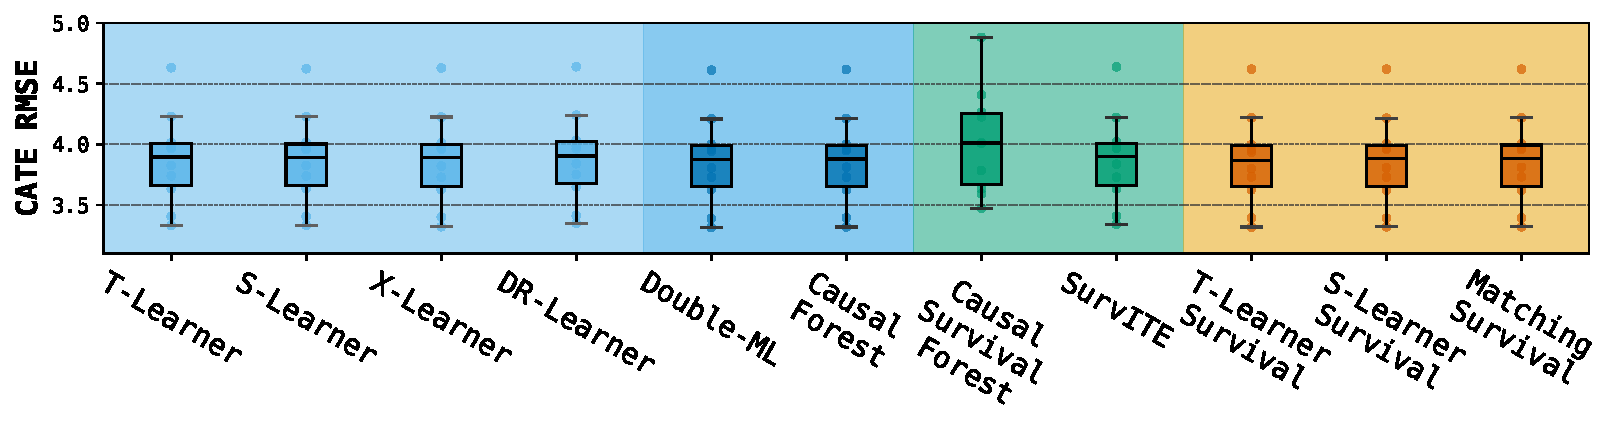
\includegraphics[width=\linewidth]{Appendices/appendix-ch04/images/figure_results_updated/cate_rmse/Scenario_A_RCT-50_cate_mse.pdf}
        
    \end{minipage}}
    \hfill
    \subfloat[{RCT: \ChFourGrayCheck (5\%), Ignorability: \ChFourGrayCheck, Positivity: \ChFourGrayCheck, Ign-Censoring: \ChFourGrayCheck}]{\begin{minipage}[t]{0.49\textwidth}
        \centering
        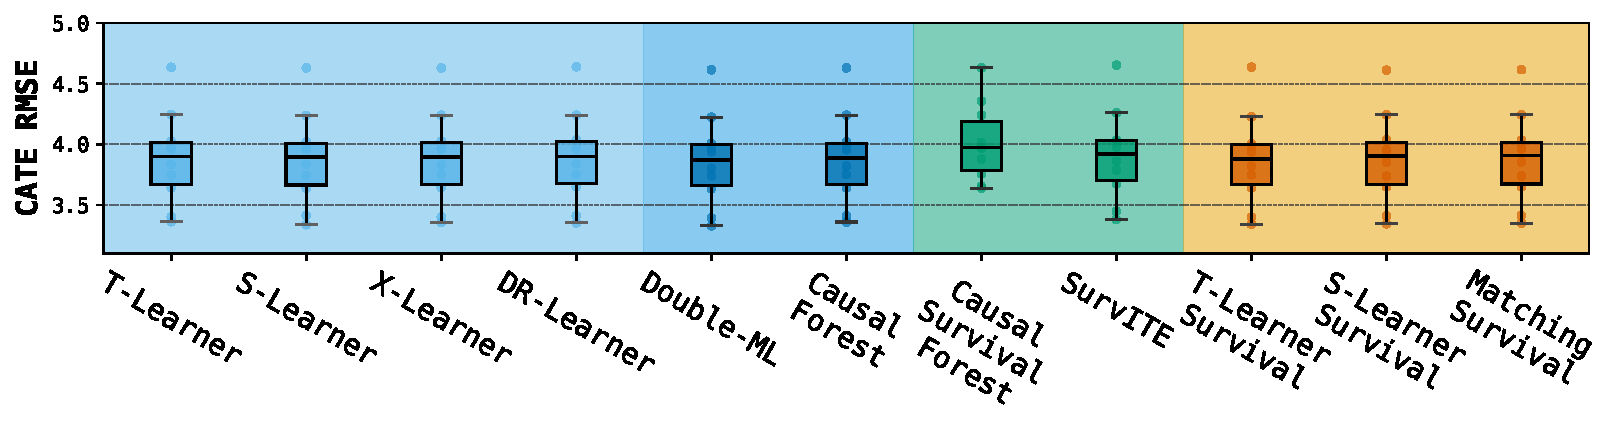
\includegraphics[width=\linewidth]{Appendices/appendix-ch04/images/figure_results_updated/cate_rmse/Scenario_A_RCT-5_cate_mse.pdf}
        
    \end{minipage}}

    

    \subfloat[{RCT: \ChFourBlackCross, Ignorability: \ChFourGrayCheck, Positivity: \ChFourGrayCheck, Ignorable Censoring: \ChFourGrayCheck}]{\begin{minipage}[t]{0.49\textwidth}
        \centering
        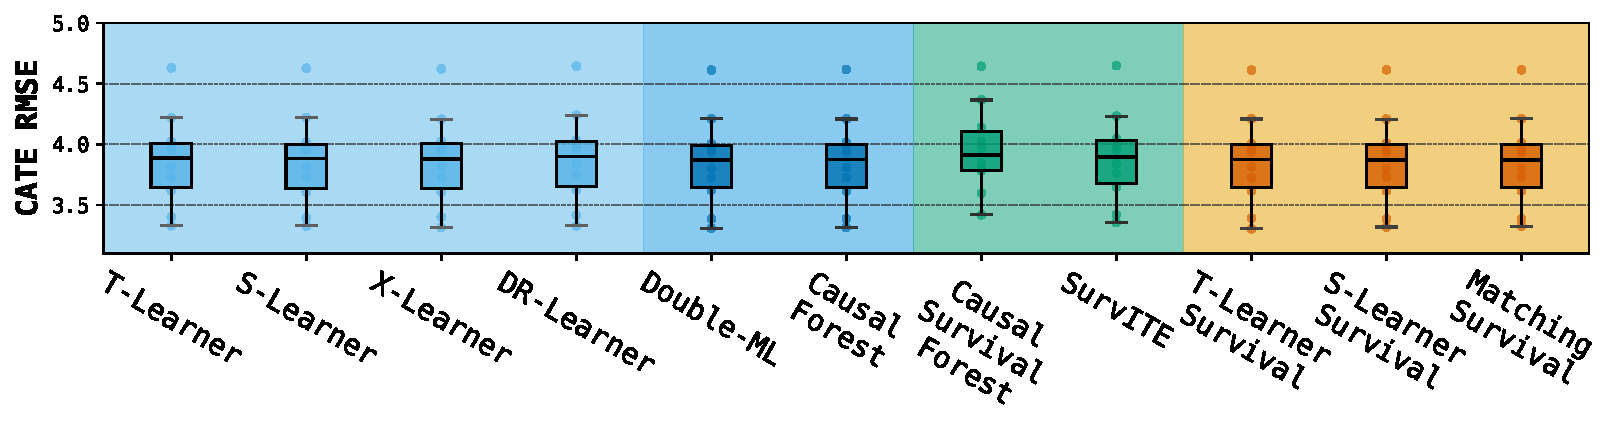
\includegraphics[width=\linewidth]{Appendices/appendix-ch04/images/figure_results_updated/cate_rmse/Scenario_A_OBS-CPS_cate_mse.pdf}
        
    \end{minipage}}
    \hfill
    \subfloat[{RCT: \ChFourBlackCross, Ignorability: \ChFourBlackCross, Positivity: \ChFourGrayCheck, Ignorable Censoring: \ChFourGrayCheck}]{\begin{minipage}[t]{0.49\textwidth}
        \centering
        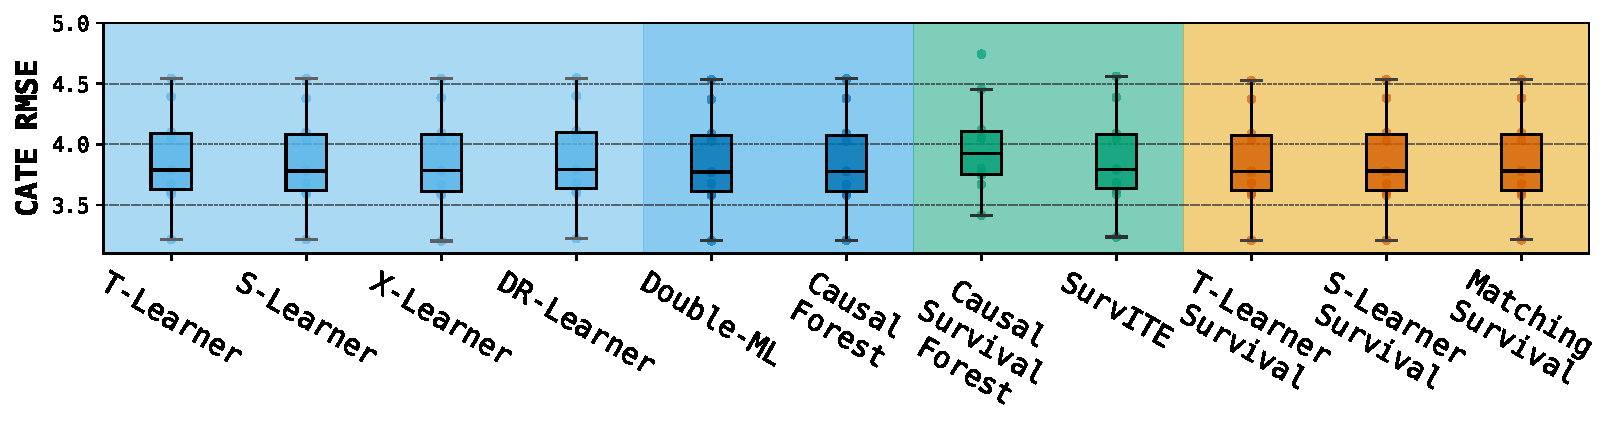
\includegraphics[width=\linewidth]{Appendices/appendix-ch04/images/figure_results_updated/cate_rmse/Scenario_A_OBS-UConf_cate_mse.pdf}
        
    \end{minipage}}

    

    \subfloat[{RCT: \ChFourBlackCross, Ignorability: \ChFourGrayCheck, Positivity: \ChFourBlackCross, Ignorable Censoring: \ChFourGrayCheck}]{\begin{minipage}[t]{0.49\textwidth}
        \centering
        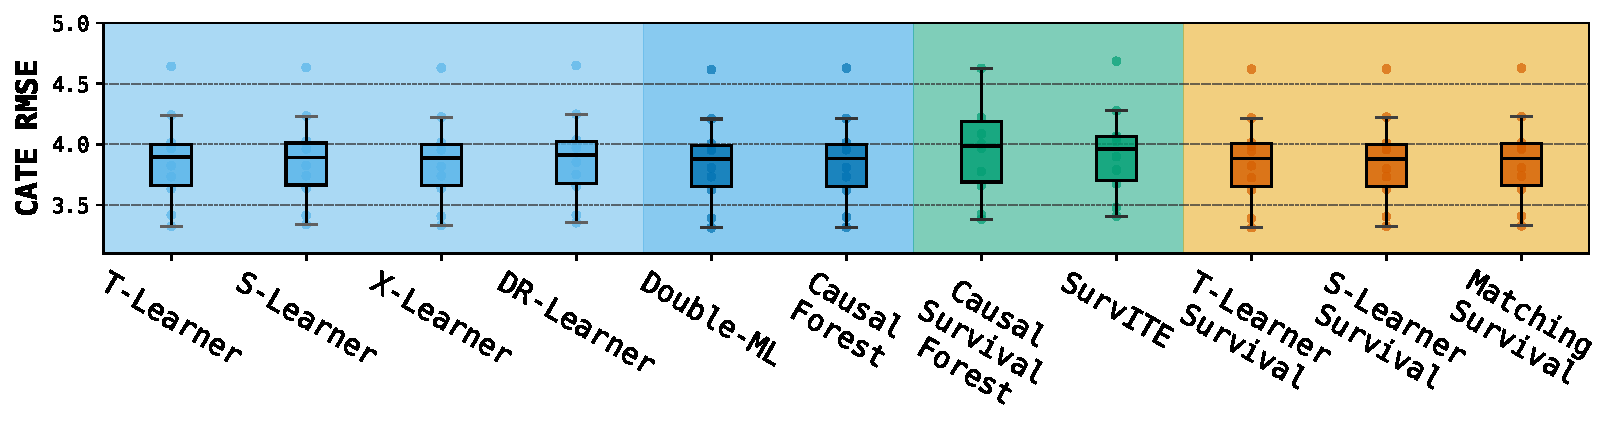
\includegraphics[width=\linewidth]{Appendices/appendix-ch04/images/figure_results_updated/cate_rmse/Scenario_A_OBS-NoPos_cate_mse.pdf}
        
    \end{minipage}}
    \hfill
    \subfloat[{RCT: \ChFourBlackCross, Ignorability: \ChFourGrayCheck, Positivity: \ChFourGrayCheck, Ignorable Censoring: \ChFourBlackCross}]{\begin{minipage}[t]{0.49\textwidth}
        \centering
        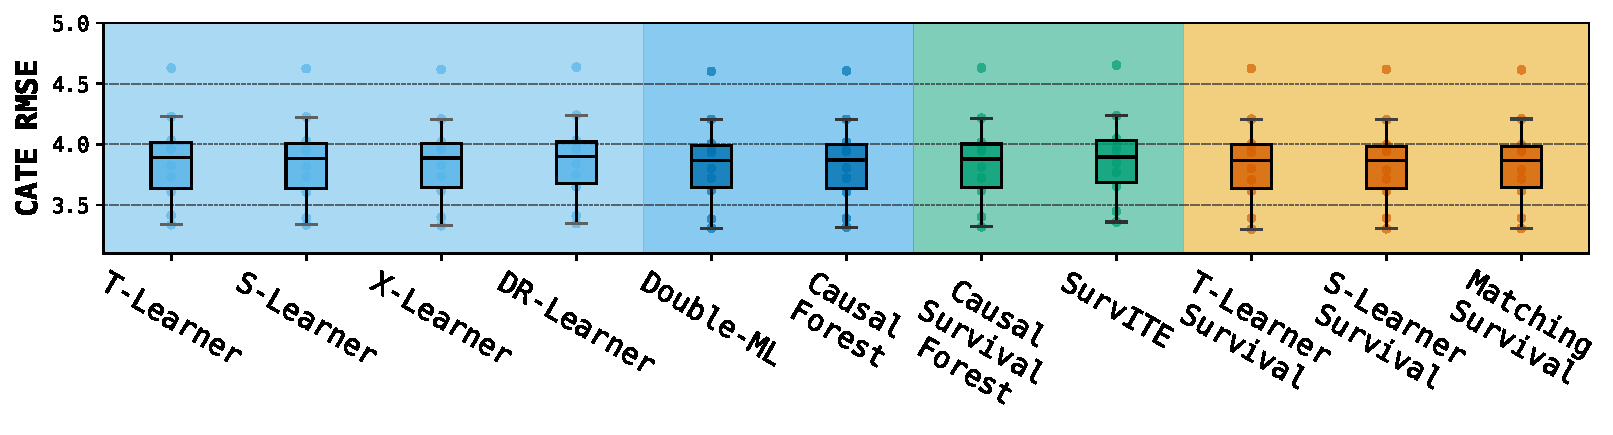
\includegraphics[width=\linewidth]{Appendices/appendix-ch04/images/figure_results_updated/cate_rmse/Scenario_A_OBS-CPS-IC_cate_mse.pdf}
        
    \end{minipage}}

    

    \subfloat[{RCT: \ChFourBlackCross, Ignorability: \ChFourBlackCross, Positivity: \ChFourGrayCheck, Ignorable Censoring: \ChFourBlackCross}]{\begin{minipage}[t]{0.49\textwidth}
        \centering
        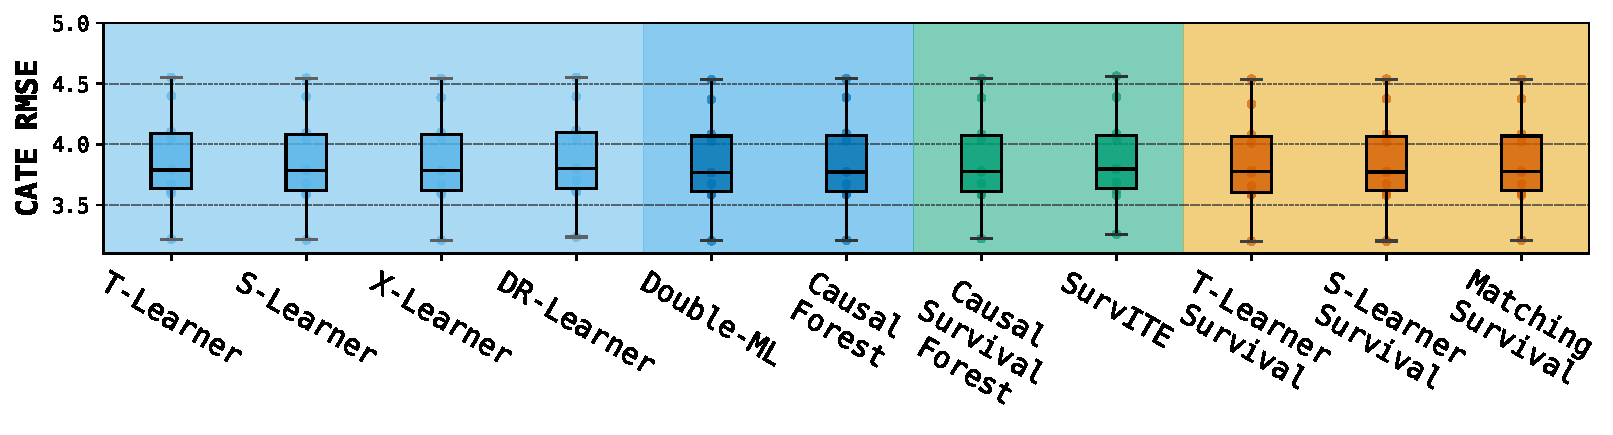
\includegraphics[width=\linewidth]{Appendices/appendix-ch04/images/figure_results_updated/cate_rmse/Scenario_A_OBS-UConf-IC_cate_mse.pdf}
        
    \end{minipage}}
    \hfill
    \subfloat[{RCT: \ChFourBlackCross, Ignorability: \ChFourGrayCheck, Positivity: \ChFourBlackCross, Ignorable Censoring: \ChFourBlackCross}]{\begin{minipage}[t]{0.49\textwidth}
        \centering
        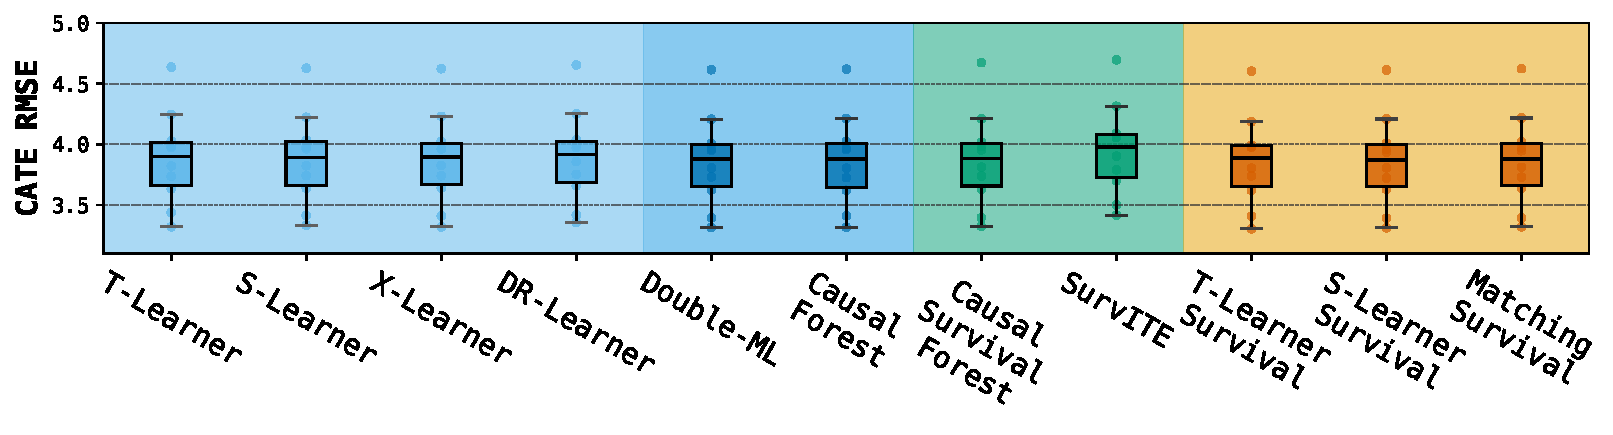
\includegraphics[width=\linewidth]{Appendices/appendix-ch04/images/figure_results_updated/cate_rmse/Scenario_A_OBS-NoPos-IC_cate_mse.pdf}
        
    \end{minipage}}

            \end{minipage}%
    }
    

    
    
}
\end{figure}


% Secnario B

% !TeX root = ../../../main.tex
\begin{figure}[htbp]
\ChFourFloatContents{ch04:fig:cate_mse_grid_scenario_B}{\caption{CATE RMSE across different experiments in Scenario \texttt{B}.}}{
    \centering

    \resizebox{0.95\textwidth}{!}{%
        \begin{minipage}{1\textwidth}


    \subfloat[{RCT: \ChFourGrayCheck (50\%), Ignorability: \ChFourGrayCheck, Positivity: \ChFourGrayCheck, Ign-Censoring: \ChFourGrayCheck}]{\begin{minipage}[t]{0.49\textwidth}
        \centering
        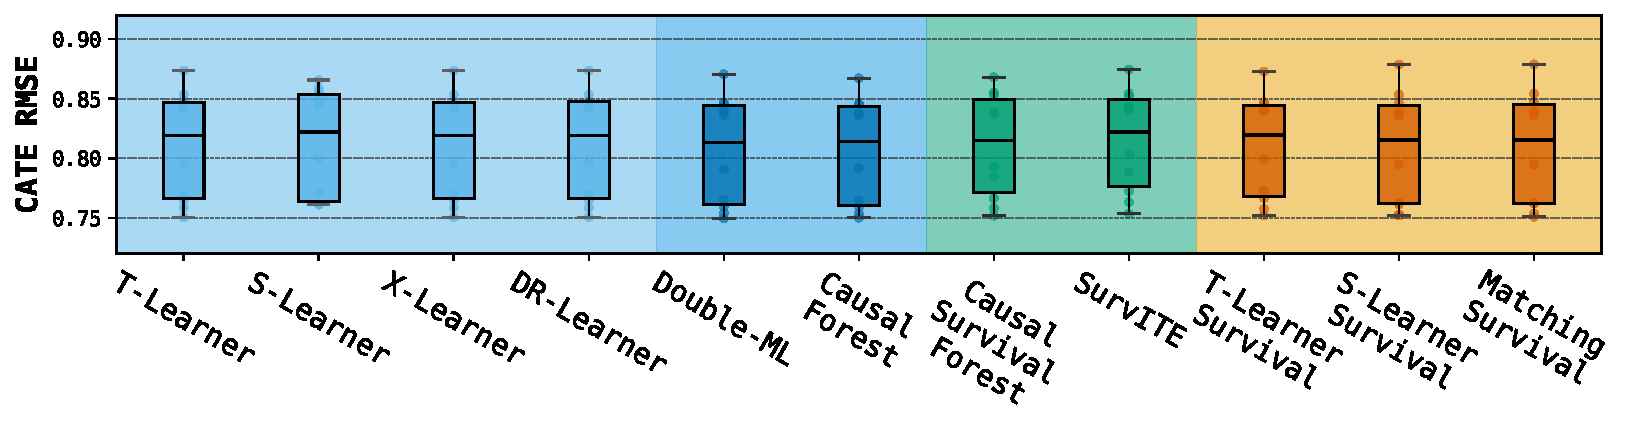
\includegraphics[width=\linewidth]{Appendices/appendix-ch04/images/figure_results_updated/cate_rmse/Scenario_B_RCT-50_cate_mse.pdf}
        
    \end{minipage}}
    \hfill
    \subfloat[{RCT: \ChFourGrayCheck (5\%), Ignorability: \ChFourGrayCheck, Positivity: \ChFourGrayCheck, Ign-Censoring: \ChFourGrayCheck}]{\begin{minipage}[t]{0.49\textwidth}
        \centering
        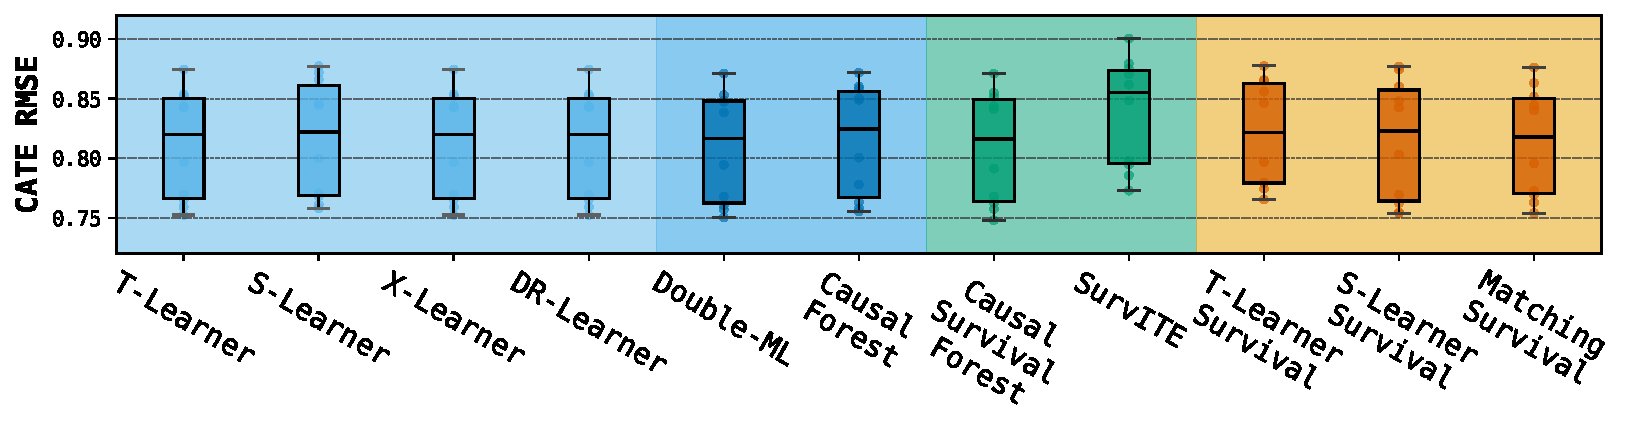
\includegraphics[width=\linewidth]{Appendices/appendix-ch04/images/figure_results_updated/cate_rmse/Scenario_B_RCT-5_cate_mse.pdf}
        
    \end{minipage}}

    

    \subfloat[{RCT: \ChFourBlackCross, Ignorability: \ChFourGrayCheck, Positivity: \ChFourGrayCheck, Ignorable Censoring: \ChFourGrayCheck}]{\begin{minipage}[t]{0.49\textwidth}
        \centering
        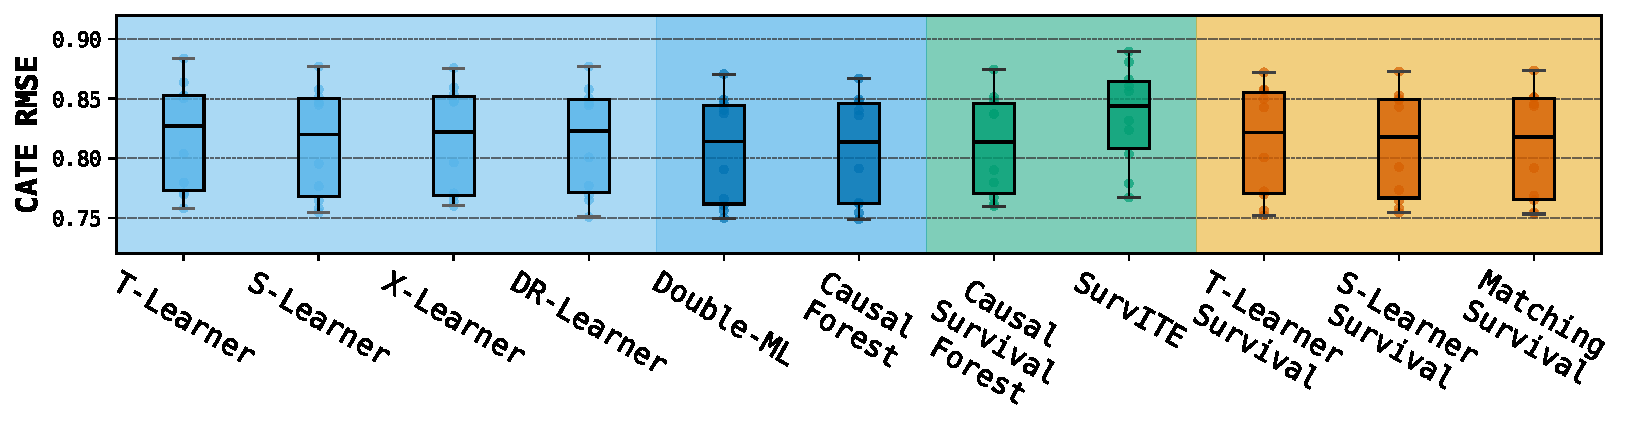
\includegraphics[width=\linewidth]{Appendices/appendix-ch04/images/figure_results_updated/cate_rmse/Scenario_B_OBS-CPS_cate_mse.pdf}
        
    \end{minipage}}
    \hfill
    \subfloat[{RCT: \ChFourBlackCross, Ignorability: \ChFourBlackCross, Positivity: \ChFourGrayCheck, Ignorable Censoring: \ChFourGrayCheck}]{\begin{minipage}[t]{0.49\textwidth}
        \centering
        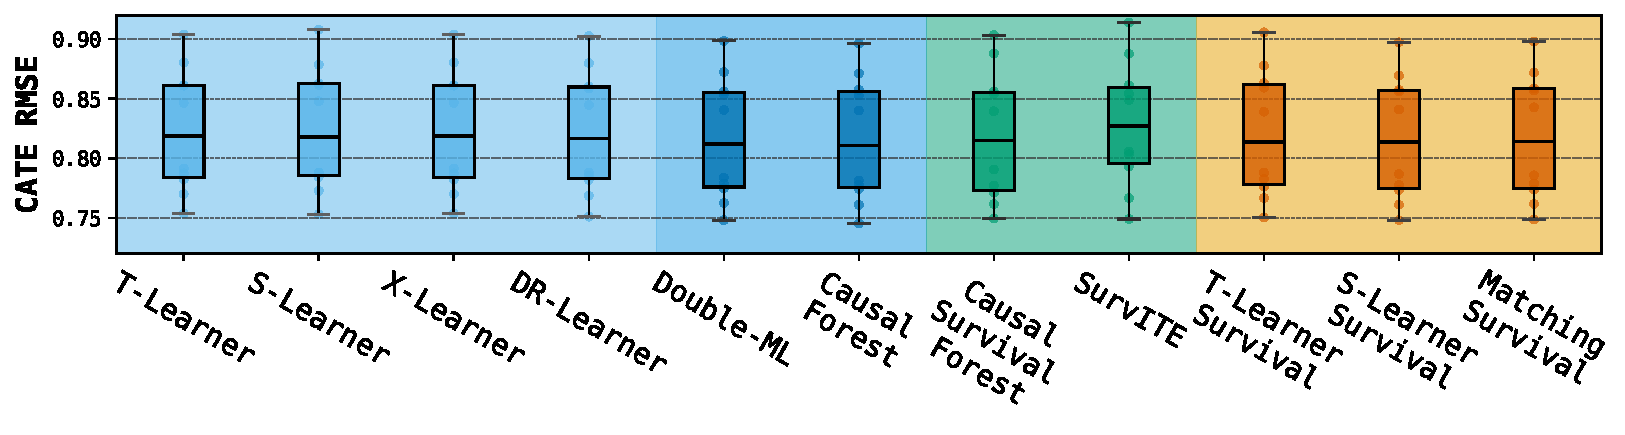
\includegraphics[width=\linewidth]{Appendices/appendix-ch04/images/figure_results_updated/cate_rmse/Scenario_B_OBS-UConf_cate_mse.pdf}
        
    \end{minipage}}

    

    \subfloat[{RCT: \ChFourBlackCross, Ignorability: \ChFourGrayCheck, Positivity: \ChFourBlackCross, Ignorable Censoring: \ChFourGrayCheck}]{\begin{minipage}[t]{0.49\textwidth}
        \centering
        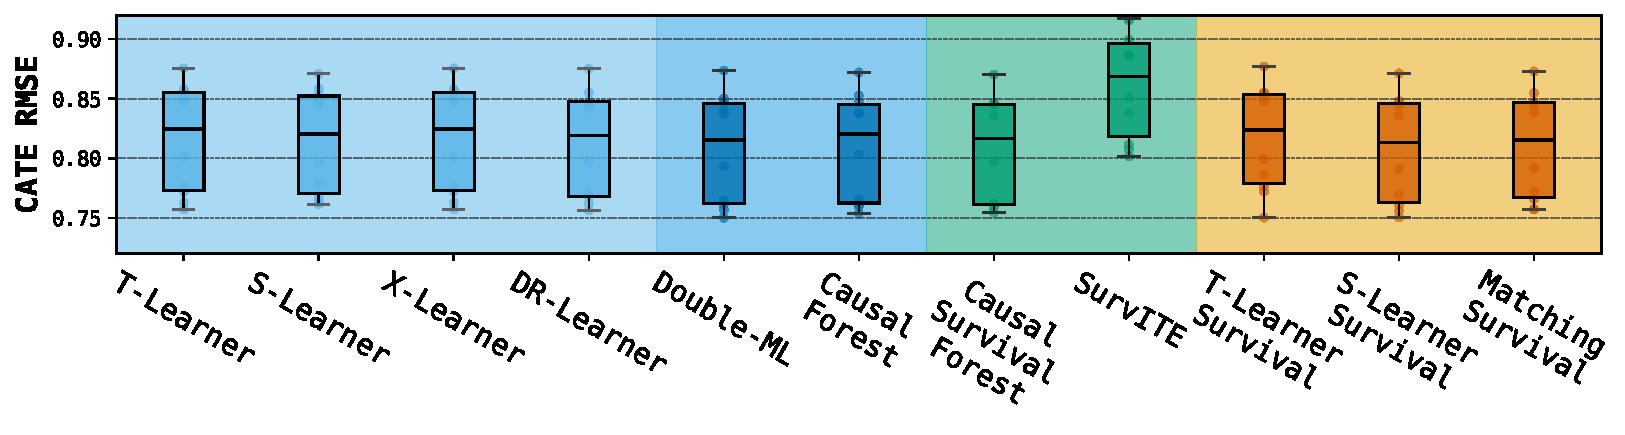
\includegraphics[width=\linewidth]{Appendices/appendix-ch04/images/figure_results_updated/cate_rmse/Scenario_B_OBS-NoPos_cate_mse.pdf}
        
    \end{minipage}}
    \hfill
    \subfloat[{RCT: \ChFourBlackCross, Ignorability: \ChFourGrayCheck, Positivity: \ChFourGrayCheck, Ignorable Censoring: \ChFourBlackCross}]{\begin{minipage}[t]{0.49\textwidth}
        \centering
        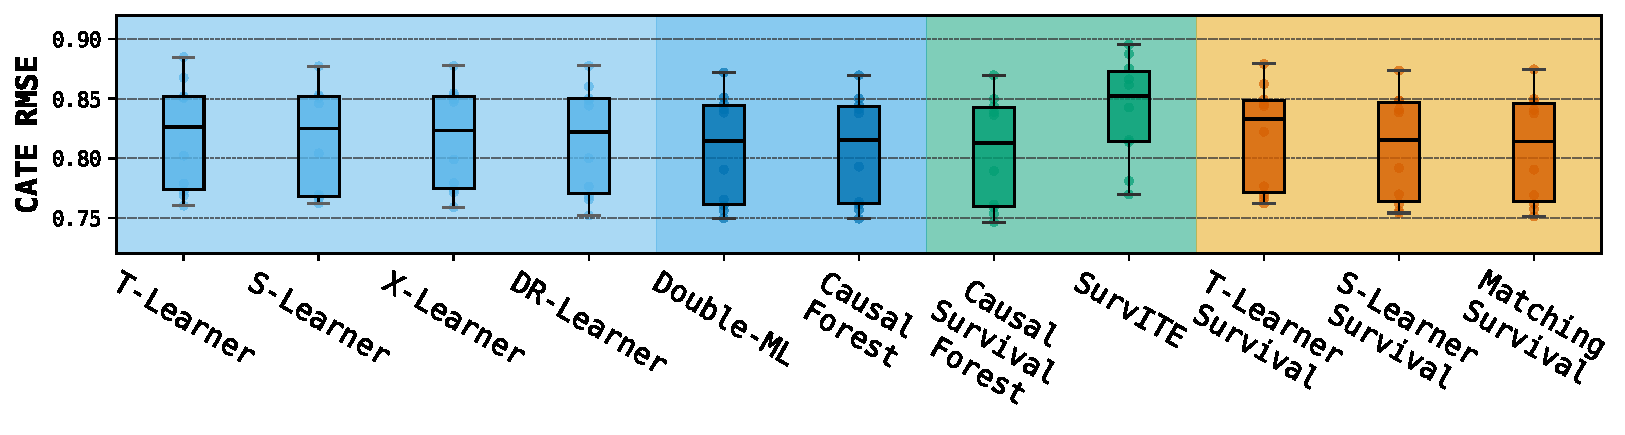
\includegraphics[width=\linewidth]{Appendices/appendix-ch04/images/figure_results_updated/cate_rmse/Scenario_B_OBS-CPS-IC_cate_mse.pdf}
        
    \end{minipage}}

    

    \subfloat[{RCT: \ChFourBlackCross, Ignorability: \ChFourBlackCross, Positivity: \ChFourGrayCheck, Ignorable Censoring: \ChFourBlackCross}]{\begin{minipage}[t]{0.49\textwidth}
        \centering
        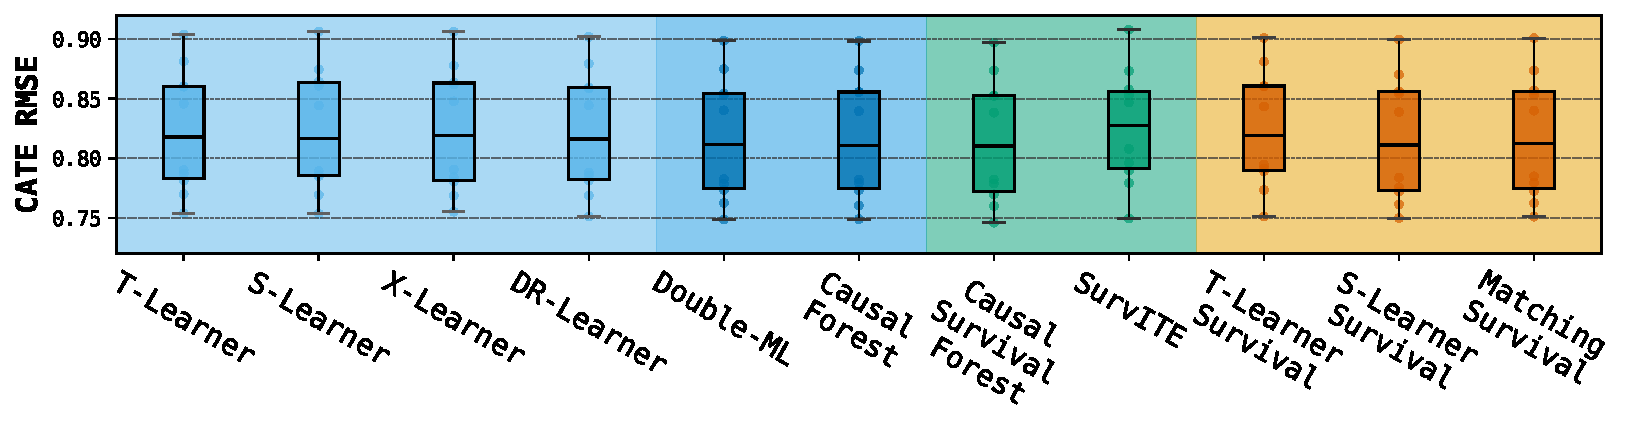
\includegraphics[width=\linewidth]{Appendices/appendix-ch04/images/figure_results_updated/cate_rmse/Scenario_B_OBS-UConf-IC_cate_mse.pdf}
        
    \end{minipage}}
    \hfill
    \subfloat[{RCT: \ChFourBlackCross, Ignorability: \ChFourGrayCheck, Positivity: \ChFourBlackCross, Ignorable Censoring: \ChFourBlackCross}]{\begin{minipage}[t]{0.49\textwidth}
        \centering
        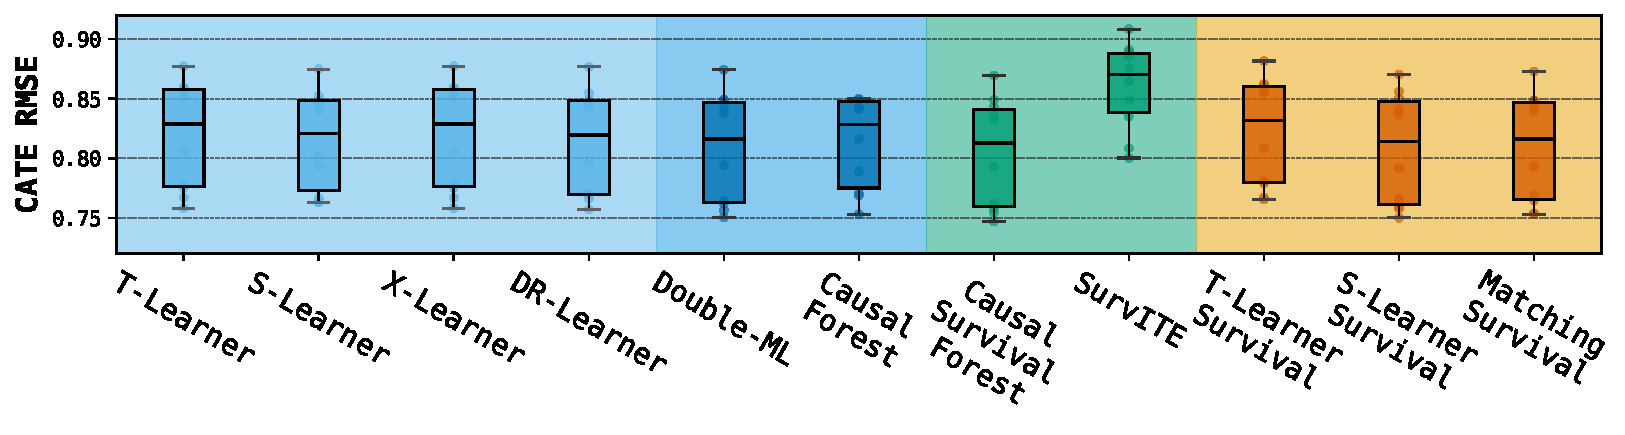
\includegraphics[width=\linewidth]{Appendices/appendix-ch04/images/figure_results_updated/cate_rmse/Scenario_B_OBS-NoPos-IC_cate_mse.pdf}
        
    \end{minipage}}

            \end{minipage}%
    }
    

    
    
}
\end{figure}



% 

% Secnario C

% !TeX root = ../../../main.tex
\begin{figure}[htbp]
\ChFourFloatContents{ch04:fig:cate_mse_grid_scenario_C}{\caption{CATE RMSE across different experiments in Scenario \texttt{C}.}}{
    \centering

    \resizebox{0.95\textwidth}{!}{%
        \begin{minipage}{1\textwidth}


    \subfloat[{RCT: \ChFourGrayCheck (50\%), Ignorability: \ChFourGrayCheck, Positivity: \ChFourGrayCheck, Ign-Censoring: \ChFourGrayCheck}]{\begin{minipage}[t]{0.49\textwidth}
        \centering
        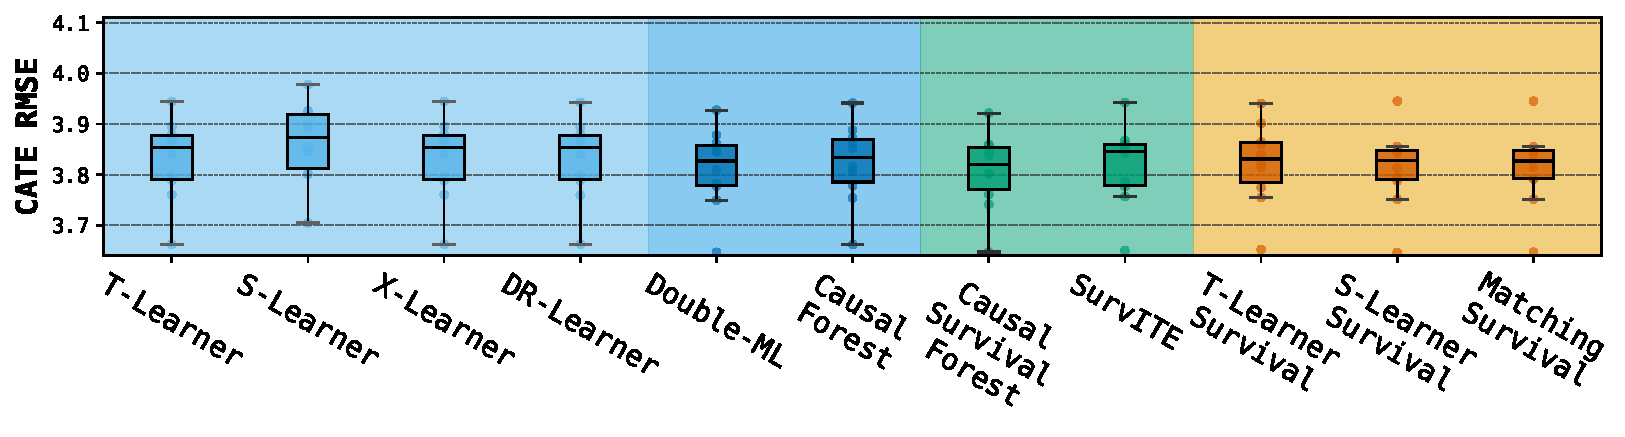
\includegraphics[width=\linewidth]{Appendices/appendix-ch04/images/figure_results_updated/cate_rmse/Scenario_C_RCT-50_cate_mse.pdf}
        
    \end{minipage}}
    \hfill
    \subfloat[{RCT: \ChFourGrayCheck (5\%), Ignorability: \ChFourGrayCheck, Positivity: \ChFourGrayCheck, Ign-Censoring: \ChFourGrayCheck}]{\begin{minipage}[t]{0.49\textwidth}
        \centering
        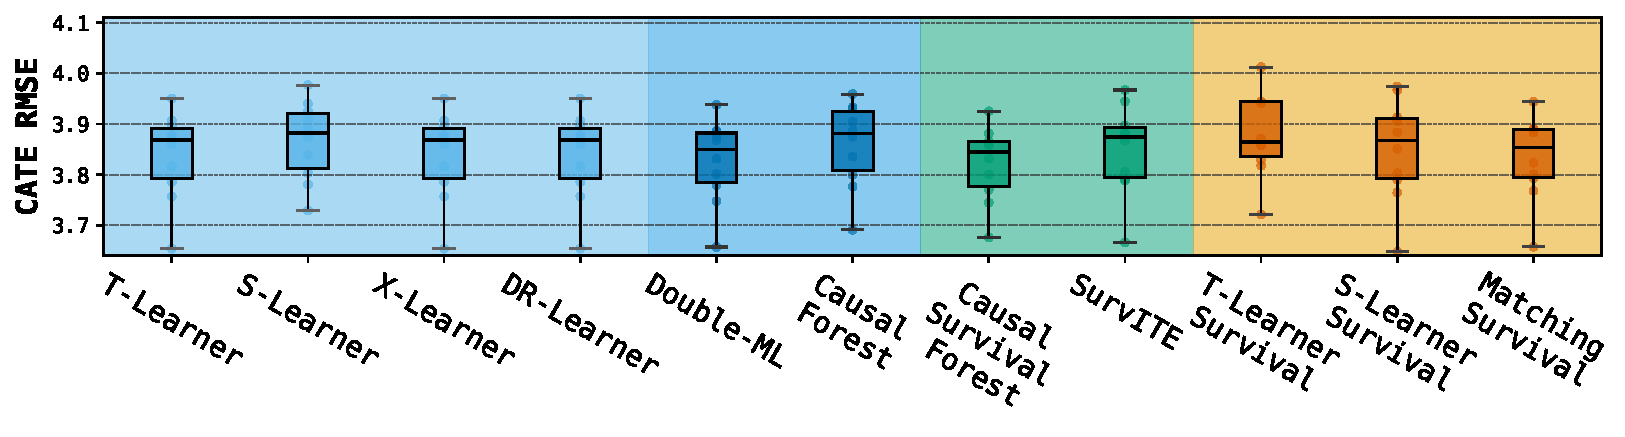
\includegraphics[width=\linewidth]{Appendices/appendix-ch04/images/figure_results_updated/cate_rmse/Scenario_C_RCT-5_cate_mse.pdf}
        
    \end{minipage}}

    

    \subfloat[{RCT: \ChFourBlackCross, Ignorability: \ChFourGrayCheck, Positivity: \ChFourGrayCheck, Ignorable Censoring: \ChFourGrayCheck}]{\begin{minipage}[t]{0.49\textwidth}
        \centering
        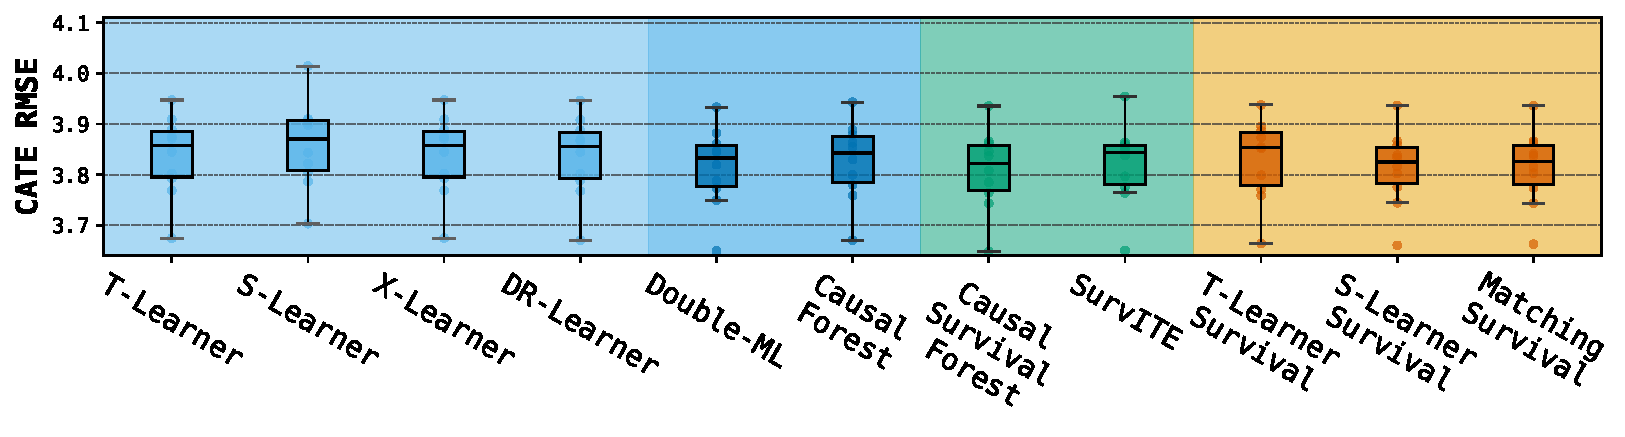
\includegraphics[width=\linewidth]{Appendices/appendix-ch04/images/figure_results_updated/cate_rmse/Scenario_C_OBS-CPS_cate_mse.pdf}
        
    \end{minipage}}
    \hfill
    \subfloat[{RCT: \ChFourBlackCross, Ignorability: \ChFourBlackCross, Positivity: \ChFourGrayCheck, Ignorable Censoring: \ChFourGrayCheck}]{\begin{minipage}[t]{0.49\textwidth}
        \centering
        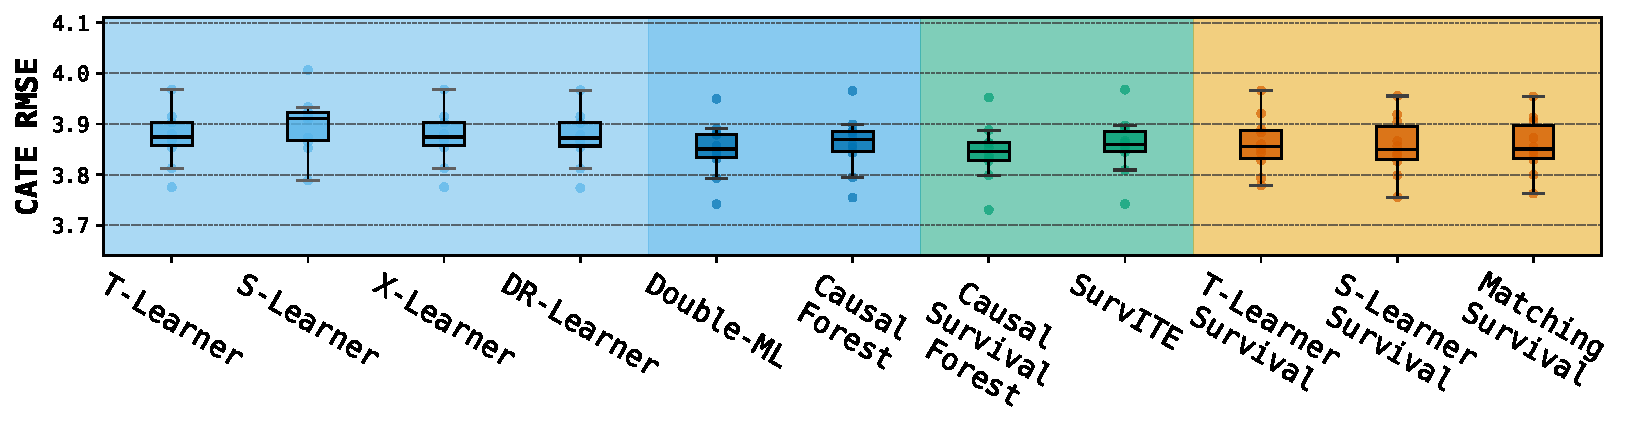
\includegraphics[width=\linewidth]{Appendices/appendix-ch04/images/figure_results_updated/cate_rmse/Scenario_C_OBS-UConf_cate_mse.pdf}
        
    \end{minipage}}

    

    \subfloat[{RCT: \ChFourBlackCross, Ignorability: \ChFourGrayCheck, Positivity: \ChFourBlackCross, Ignorable Censoring: \ChFourGrayCheck}]{\begin{minipage}[t]{0.49\textwidth}
        \centering
        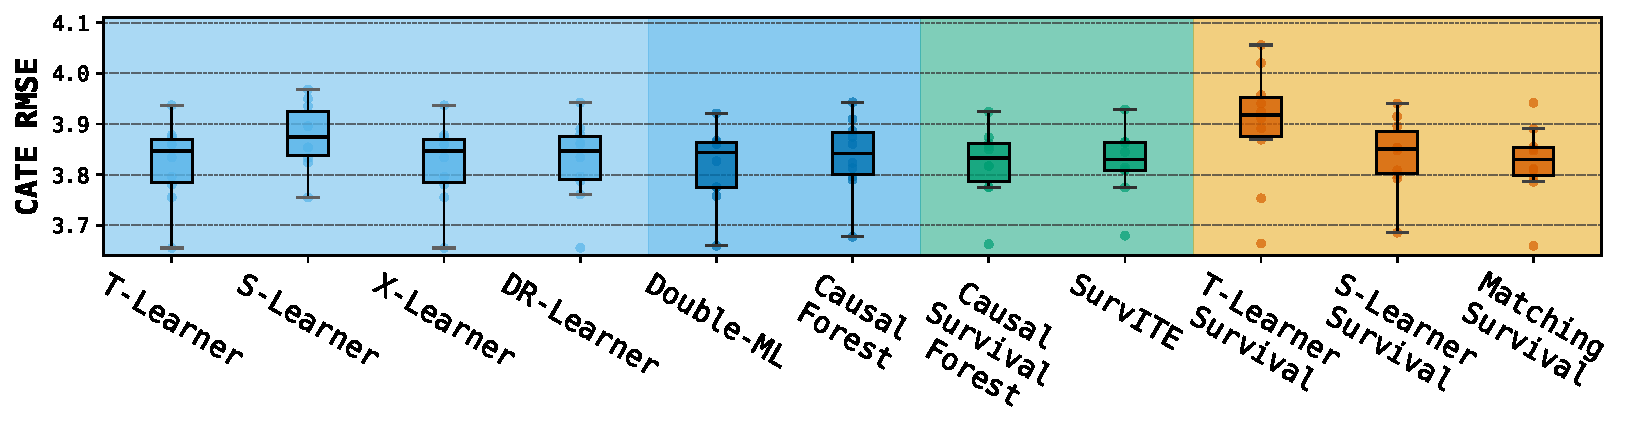
\includegraphics[width=\linewidth]{Appendices/appendix-ch04/images/figure_results_updated/cate_rmse/Scenario_C_OBS-NoPos_cate_mse.pdf}
        
    \end{minipage}}
    \hfill
    \subfloat[{RCT: \ChFourBlackCross, Ignorability: \ChFourGrayCheck, Positivity: \ChFourGrayCheck, Ignorable Censoring: \ChFourBlackCross}]{\begin{minipage}[t]{0.49\textwidth}
        \centering
        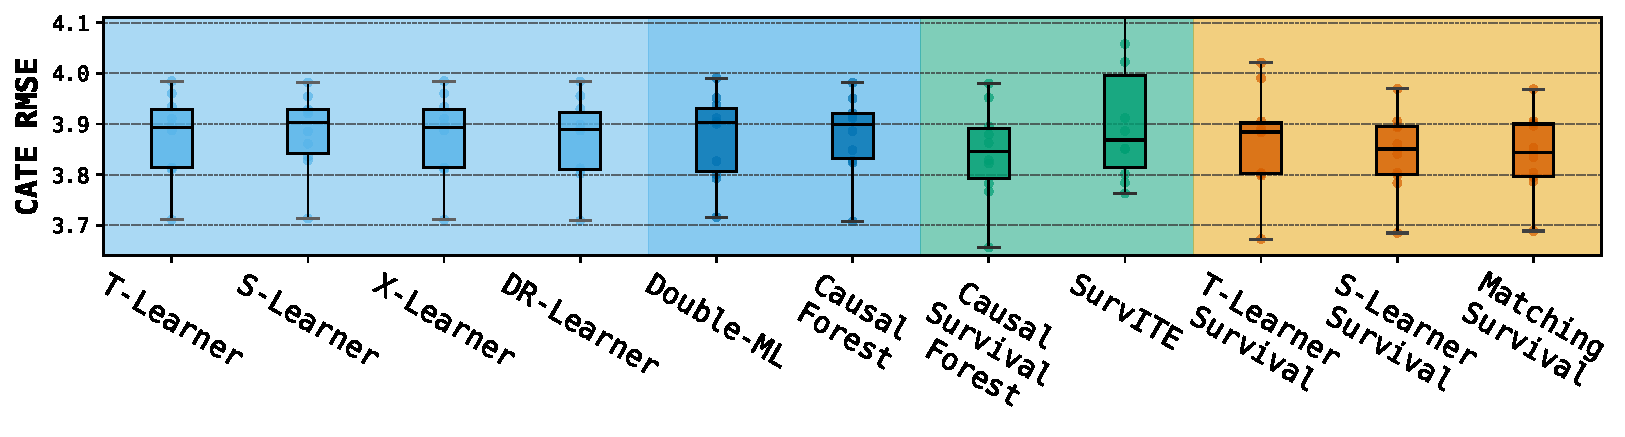
\includegraphics[width=\linewidth]{Appendices/appendix-ch04/images/figure_results_updated/cate_rmse/Scenario_C_OBS-CPS-IC_cate_mse.pdf}
        
    \end{minipage}}

    

    \subfloat[{RCT: \ChFourBlackCross, Ignorability: \ChFourBlackCross, Positivity: \ChFourGrayCheck, Ignorable Censoring: \ChFourBlackCross}]{\begin{minipage}[t]{0.49\textwidth}
        \centering
        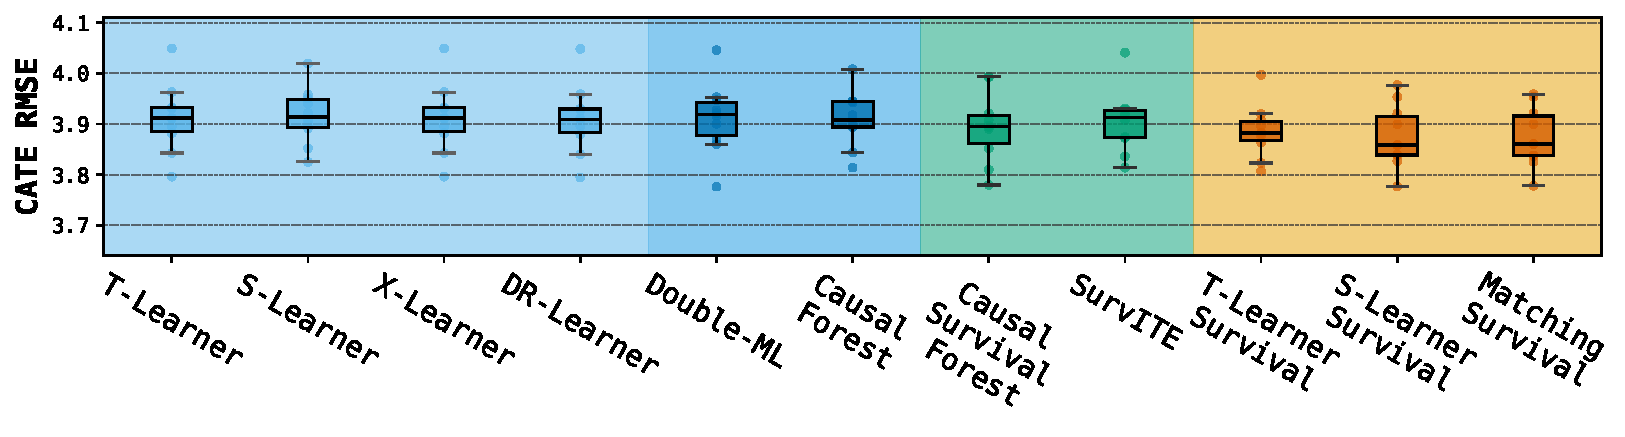
\includegraphics[width=\linewidth]{Appendices/appendix-ch04/images/figure_results_updated/cate_rmse/Scenario_C_OBS-UConf-IC_cate_mse.pdf}
        
    \end{minipage}}
    \hfill
    \subfloat[{RCT: \ChFourBlackCross, Ignorability: \ChFourGrayCheck, Positivity: \ChFourBlackCross, Ignorable Censoring: \ChFourBlackCross}]{\begin{minipage}[t]{0.49\textwidth}
        \centering
        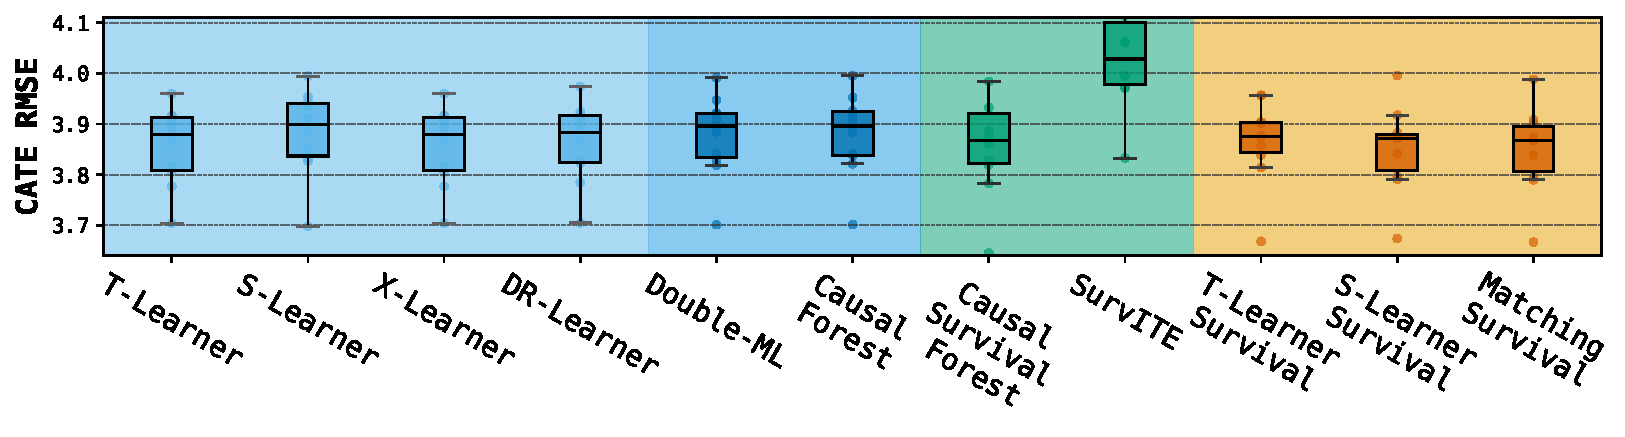
\includegraphics[width=\linewidth]{Appendices/appendix-ch04/images/figure_results_updated/cate_rmse/Scenario_C_OBS-NoPos-IC_cate_mse.pdf}
        
    \end{minipage}}

            \end{minipage}%
    }
    

    
    
}
\end{figure}




% 

% Scenario D

% !TeX root = ../../../main.tex
\begin{figure}[htbp]
\ChFourFloatContents{ch04:fig:cate_mse_grid_scenario_D}{\caption{CATE RMSE across different experiments in Scenario \texttt{D}.}}{
    \centering

    \resizebox{0.95\textwidth}{!}{%
        \begin{minipage}{1\textwidth}


    \subfloat[{RCT: \ChFourGrayCheck (50\%), Ignorability: \ChFourGrayCheck, Positivity: \ChFourGrayCheck, Ign-Censoring: \ChFourGrayCheck}]{\begin{minipage}[t]{0.49\textwidth}
        \centering
        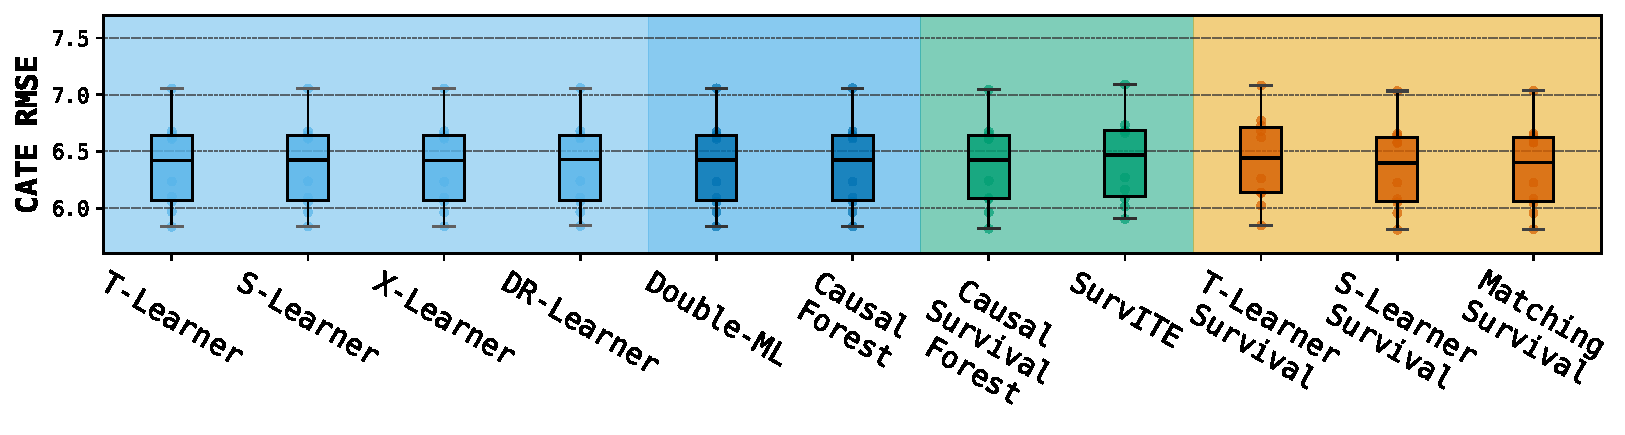
\includegraphics[width=\linewidth]{Appendices/appendix-ch04/images/figure_results_updated/cate_rmse/Scenario_D_RCT-50_cate_mse.pdf}
        
    \end{minipage}}
    \hfill
    \subfloat[{RCT: \ChFourGrayCheck (5\%), Ignorability: \ChFourGrayCheck, Positivity: \ChFourGrayCheck, Ign-Censoring: \ChFourGrayCheck}]{\begin{minipage}[t]{0.49\textwidth}
        \centering
        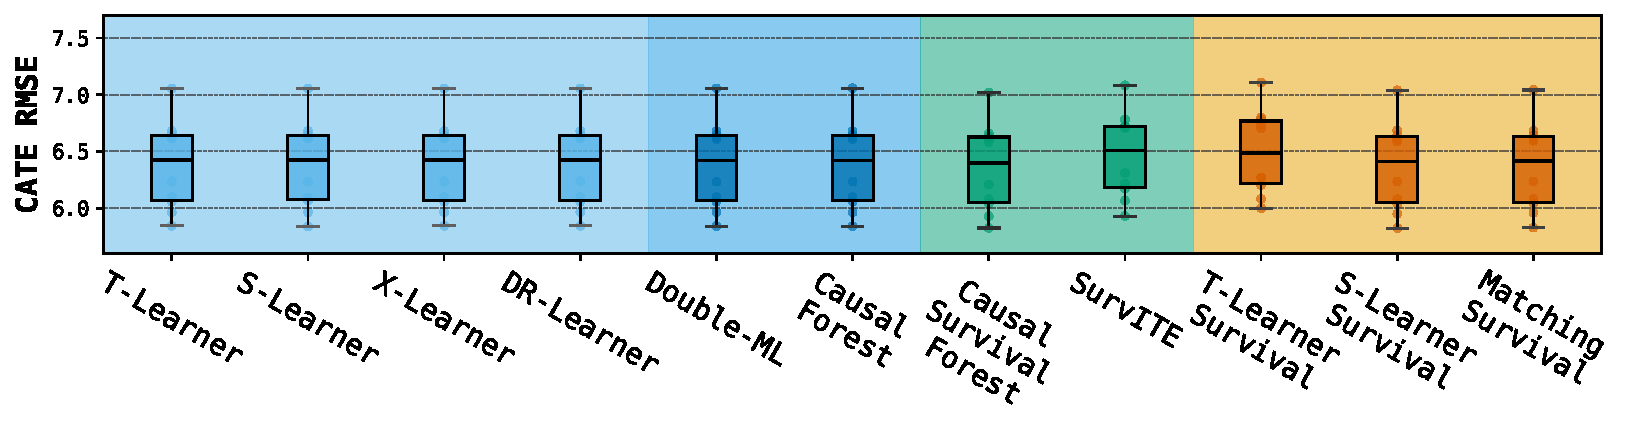
\includegraphics[width=\linewidth]{Appendices/appendix-ch04/images/figure_results_updated/cate_rmse/Scenario_D_RCT-5_cate_mse.pdf}
        
    \end{minipage}}

    

    \subfloat[{RCT: \ChFourBlackCross, Ignorability: \ChFourGrayCheck, Positivity: \ChFourGrayCheck, Ignorable Censoring: \ChFourGrayCheck}]{\begin{minipage}[t]{0.49\textwidth}
        \centering
        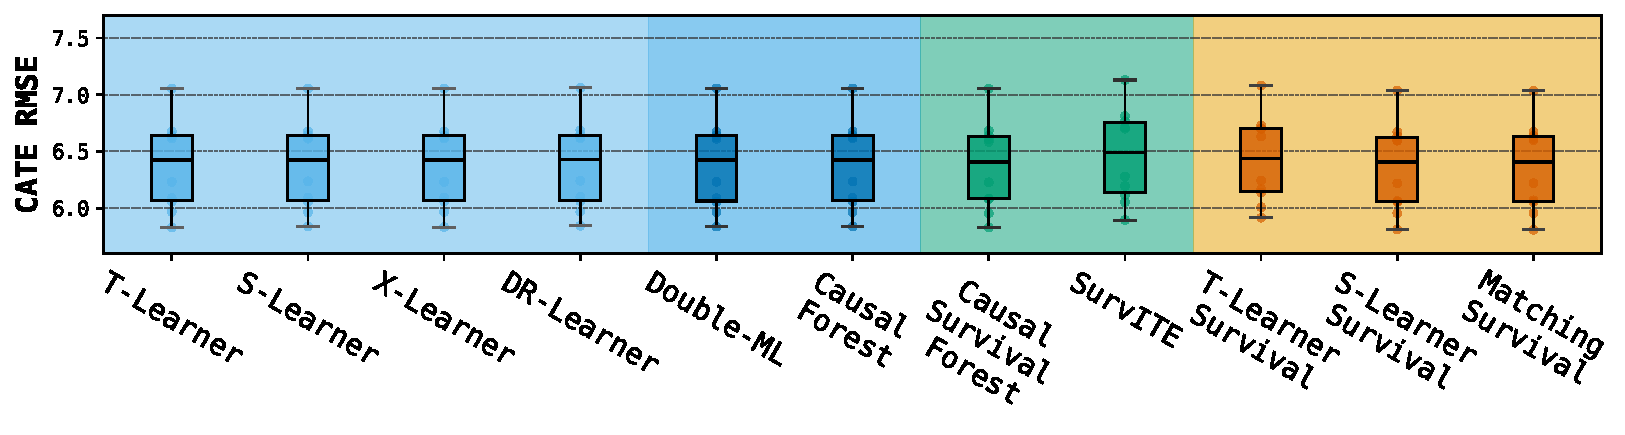
\includegraphics[width=\linewidth]{Appendices/appendix-ch04/images/figure_results_updated/cate_rmse/Scenario_D_OBS-CPS_cate_mse.pdf}
        
    \end{minipage}}
    \hfill
    \subfloat[{RCT: \ChFourBlackCross, Ignorability: \ChFourBlackCross, Positivity: \ChFourGrayCheck, Ignorable Censoring: \ChFourGrayCheck}]{\begin{minipage}[t]{0.49\textwidth}
        \centering
        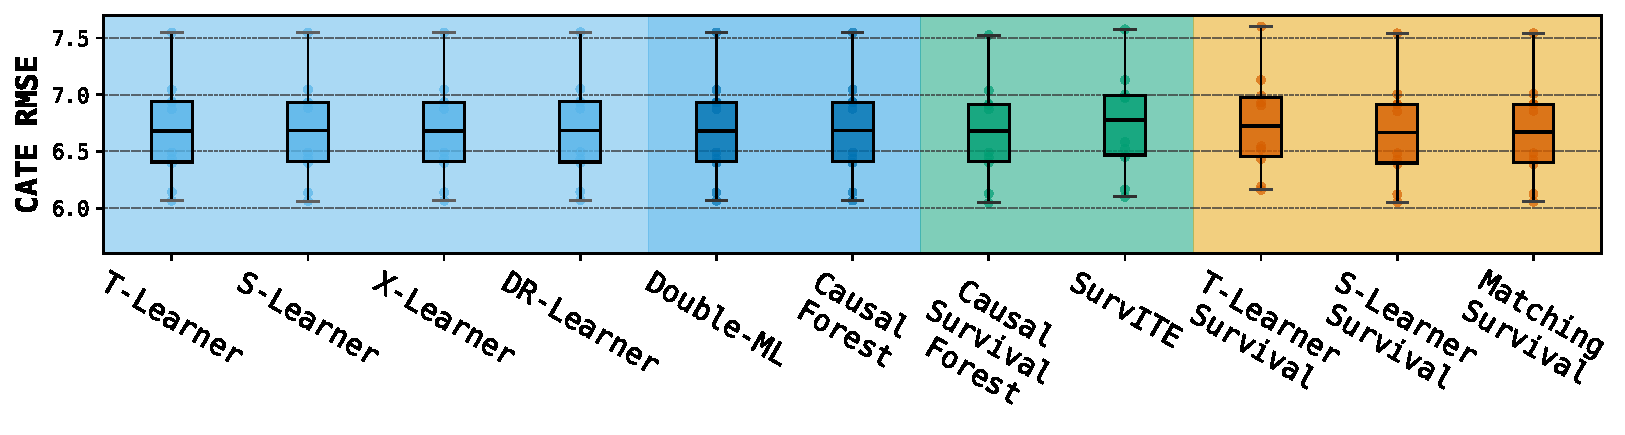
\includegraphics[width=\linewidth]{Appendices/appendix-ch04/images/figure_results_updated/cate_rmse/Scenario_D_OBS-UConf_cate_mse.pdf}
        
    \end{minipage}}

    

    \subfloat[{RCT: \ChFourBlackCross, Ignorability: \ChFourGrayCheck, Positivity: \ChFourBlackCross, Ignorable Censoring: \ChFourGrayCheck}]{\begin{minipage}[t]{0.49\textwidth}
        \centering
        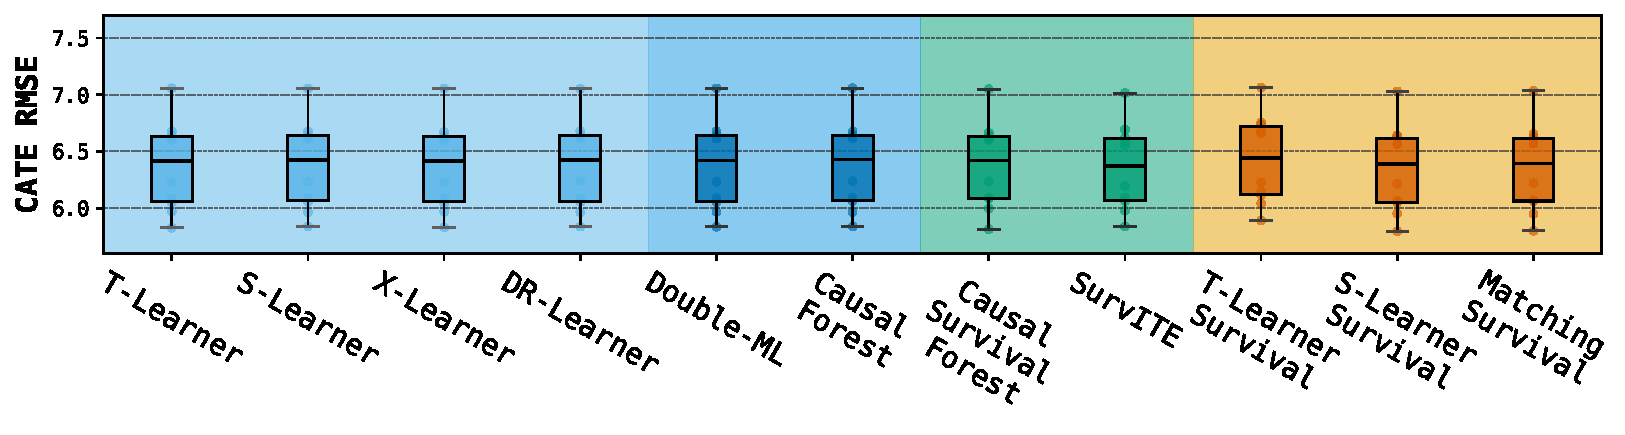
\includegraphics[width=\linewidth]{Appendices/appendix-ch04/images/figure_results_updated/cate_rmse/Scenario_D_OBS-NoPos_cate_mse.pdf}
        
    \end{minipage}}
    \hfill
    \subfloat[{RCT: \ChFourBlackCross, Ignorability: \ChFourGrayCheck, Positivity: \ChFourGrayCheck, Ignorable Censoring: \ChFourBlackCross}]{\begin{minipage}[t]{0.49\textwidth}
        \centering
        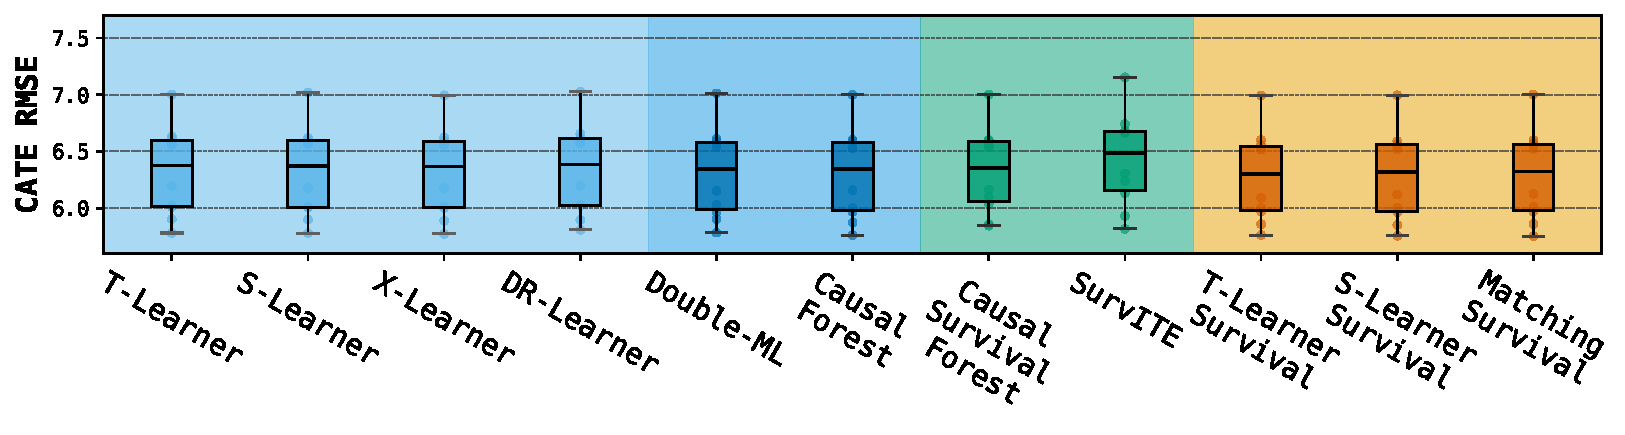
\includegraphics[width=\linewidth]{Appendices/appendix-ch04/images/figure_results_updated/cate_rmse/Scenario_D_OBS-CPS-IC_cate_mse.pdf}
        
    \end{minipage}}

    

    \subfloat[{RCT: \ChFourBlackCross, Ignorability: \ChFourBlackCross, Positivity: \ChFourGrayCheck, Ignorable Censoring: \ChFourBlackCross}]{\begin{minipage}[t]{0.49\textwidth}
        \centering
        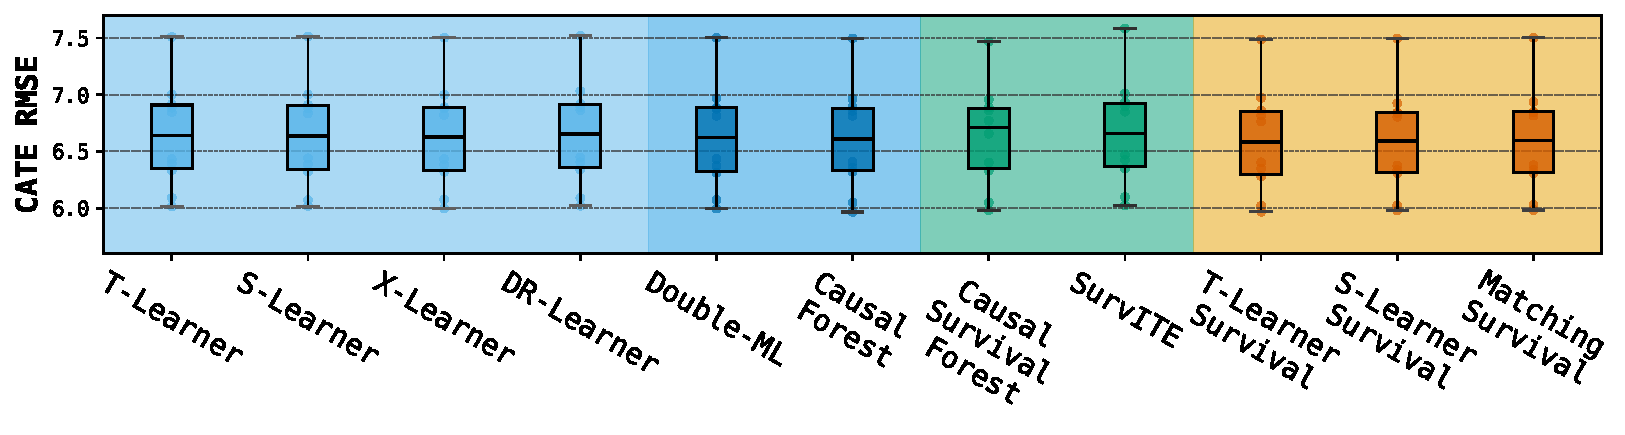
\includegraphics[width=\linewidth]{Appendices/appendix-ch04/images/figure_results_updated/cate_rmse/Scenario_D_OBS-UConf-IC_cate_mse.pdf}
        
    \end{minipage}}
    \hfill
    \subfloat[{RCT: \ChFourBlackCross, Ignorability: \ChFourGrayCheck, Positivity: \ChFourBlackCross, Ignorable Censoring: \ChFourBlackCross}]{\begin{minipage}[t]{0.49\textwidth}
        \centering
        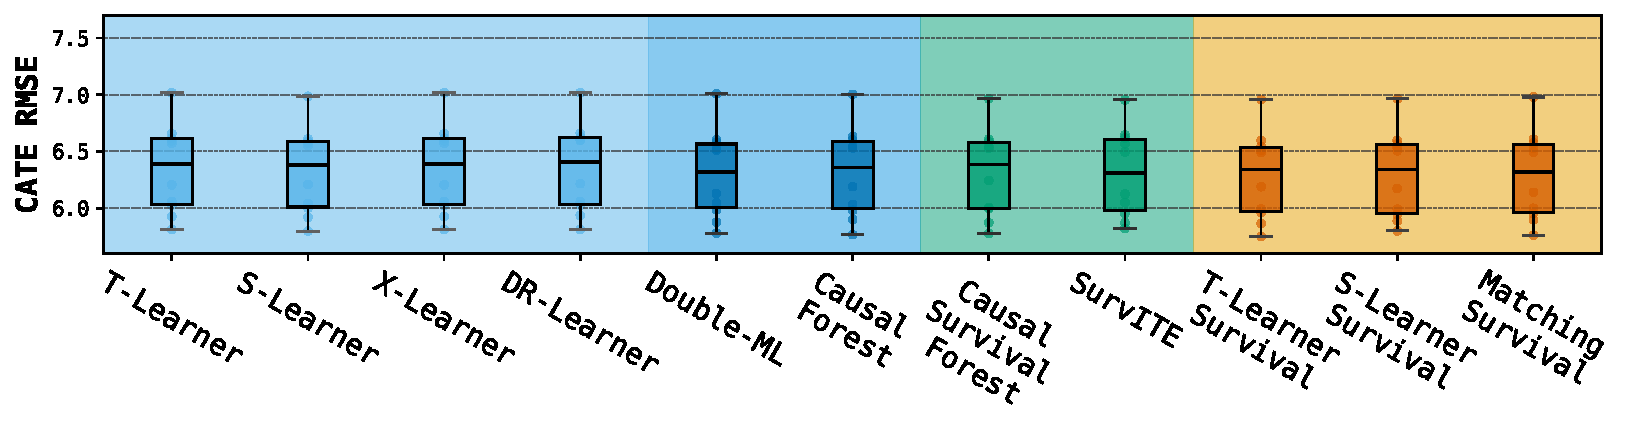
\includegraphics[width=\linewidth]{Appendices/appendix-ch04/images/figure_results_updated/cate_rmse/Scenario_D_OBS-NoPos-IC_cate_mse.pdf}
        
    \end{minipage}}

            \end{minipage}%
    }
    

    
    
}
\end{figure}


% 

% Secnario E

% !TeX root = ../../../main.tex
\begin{figure}[htbp]
\ChFourFloatContents{ch04:fig:cate_mse_grid_scenario_E}{\caption{CATE RMSE across different experiments in Scenario \texttt{E}.}}{
    \centering

    \resizebox{0.95\textwidth}{!}{%
        \begin{minipage}{1\textwidth}


    \subfloat[{RCT: \ChFourGrayCheck (50\%), Ignorability: \ChFourGrayCheck, Positivity: \ChFourGrayCheck, Ign-Censoring: \ChFourGrayCheck}]{\begin{minipage}[t]{0.49\textwidth}
        \centering
        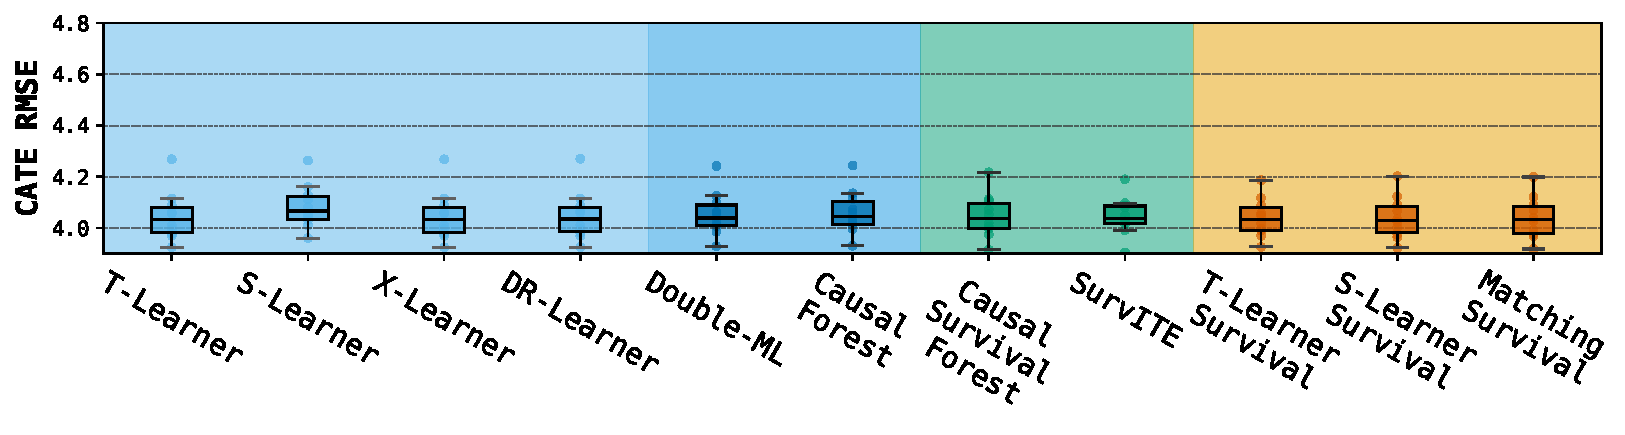
\includegraphics[width=\linewidth]{Appendices/appendix-ch04/images/figure_results_updated/cate_rmse/Scenario_E_RCT-50_cate_mse.pdf}
        
    \end{minipage}}
    \hfill
    \subfloat[{RCT: \ChFourGrayCheck (5\%), Ignorability: \ChFourGrayCheck, Positivity: \ChFourGrayCheck, Ign-Censoring: \ChFourGrayCheck}]{\begin{minipage}[t]{0.49\textwidth}
        \centering
        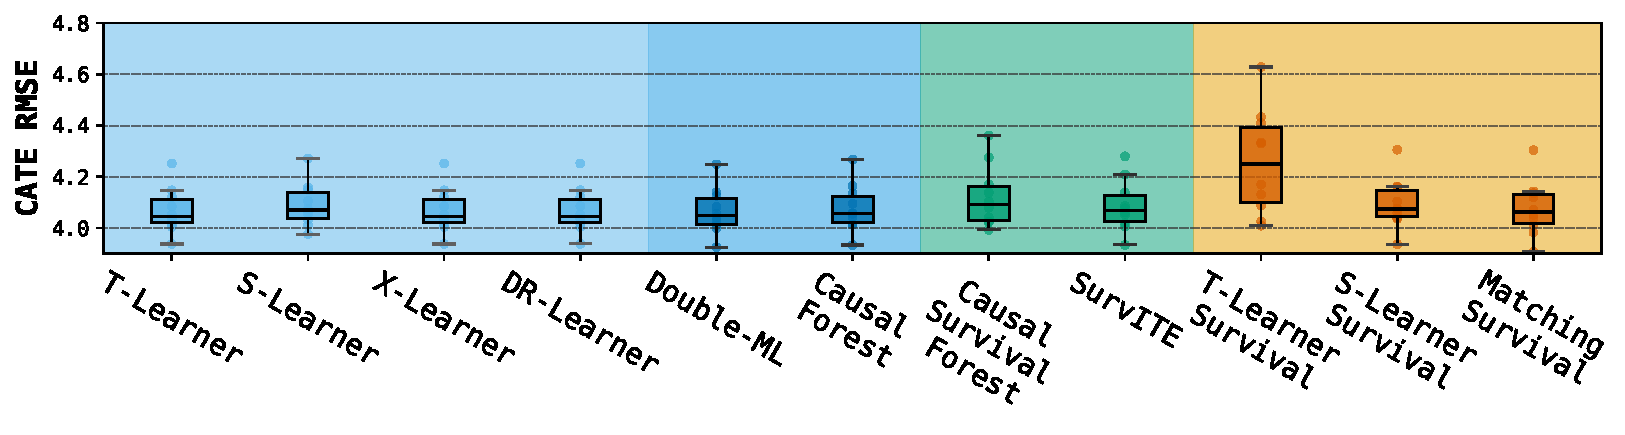
\includegraphics[width=\linewidth]{Appendices/appendix-ch04/images/figure_results_updated/cate_rmse/Scenario_E_RCT-5_cate_mse.pdf}
        
    \end{minipage}}

    

    \subfloat[{RCT: \ChFourBlackCross, Ignorability: \ChFourGrayCheck, Positivity: \ChFourGrayCheck, Ignorable Censoring: \ChFourGrayCheck}]{\begin{minipage}[t]{0.49\textwidth}
        \centering
        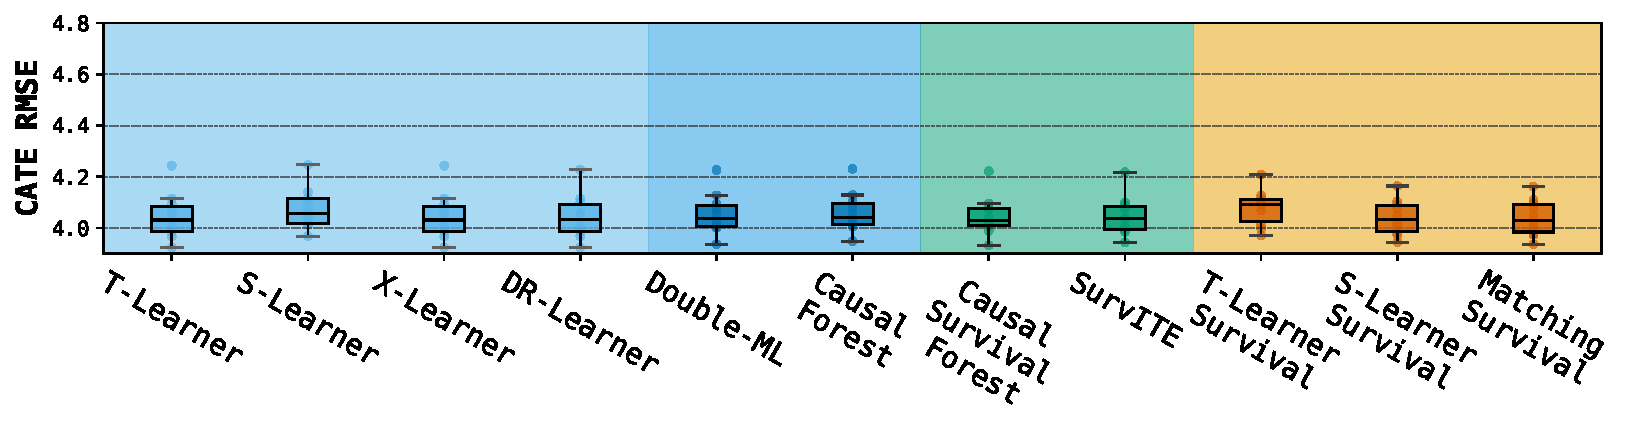
\includegraphics[width=\linewidth]{Appendices/appendix-ch04/images/figure_results_updated/cate_rmse/Scenario_E_OBS-CPS_cate_mse.pdf}
        
    \end{minipage}}
    \hfill
    \subfloat[{RCT: \ChFourBlackCross, Ignorability: \ChFourBlackCross, Positivity: \ChFourGrayCheck, Ignorable Censoring: \ChFourGrayCheck}]{\begin{minipage}[t]{0.49\textwidth}
        \centering
        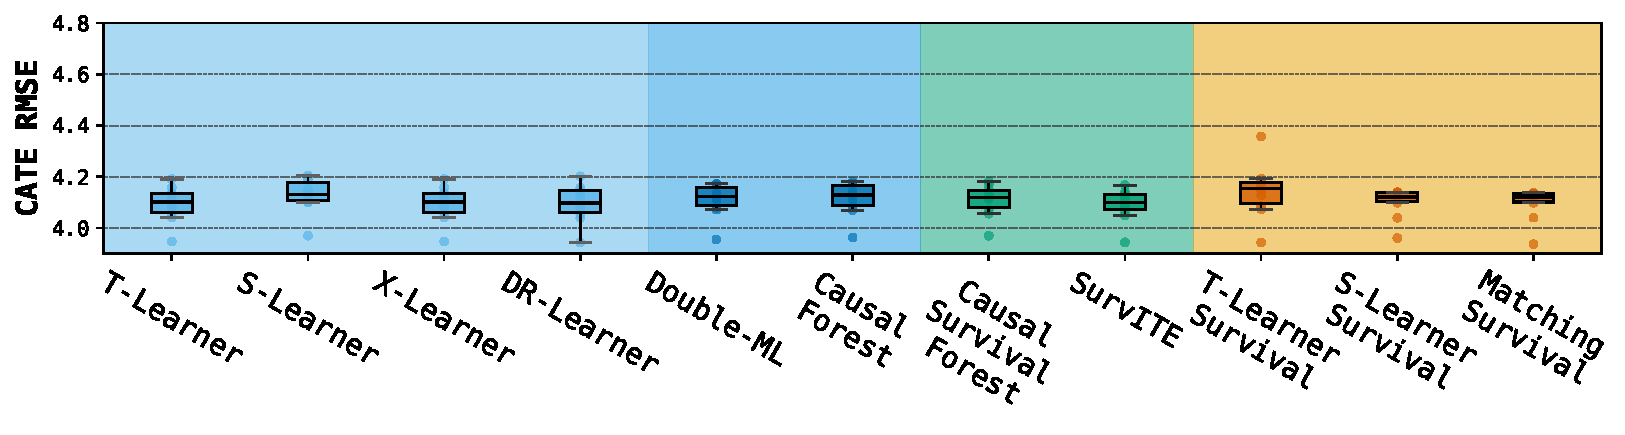
\includegraphics[width=\linewidth]{Appendices/appendix-ch04/images/figure_results_updated/cate_rmse/Scenario_E_OBS-UConf_cate_mse.pdf}
        
    \end{minipage}}

    

    \subfloat[{RCT: \ChFourBlackCross, Ignorability: \ChFourGrayCheck, Positivity: \ChFourBlackCross, Ignorable Censoring: \ChFourGrayCheck}]{\begin{minipage}[t]{0.49\textwidth}
        \centering
        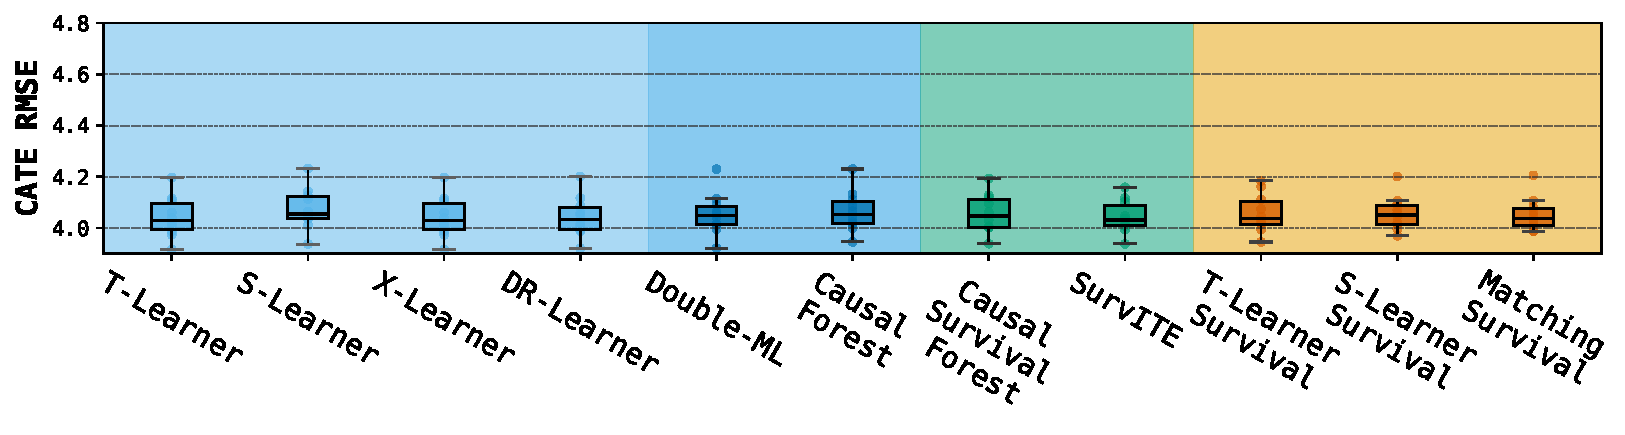
\includegraphics[width=\linewidth]{Appendices/appendix-ch04/images/figure_results_updated/cate_rmse/Scenario_E_OBS-NoPos_cate_mse.pdf}
        
    \end{minipage}}
    \hfill
    \subfloat[{RCT: \ChFourBlackCross, Ignorability: \ChFourGrayCheck, Positivity: \ChFourGrayCheck, Ignorable Censoring: \ChFourBlackCross}]{\begin{minipage}[t]{0.49\textwidth}
        \centering
        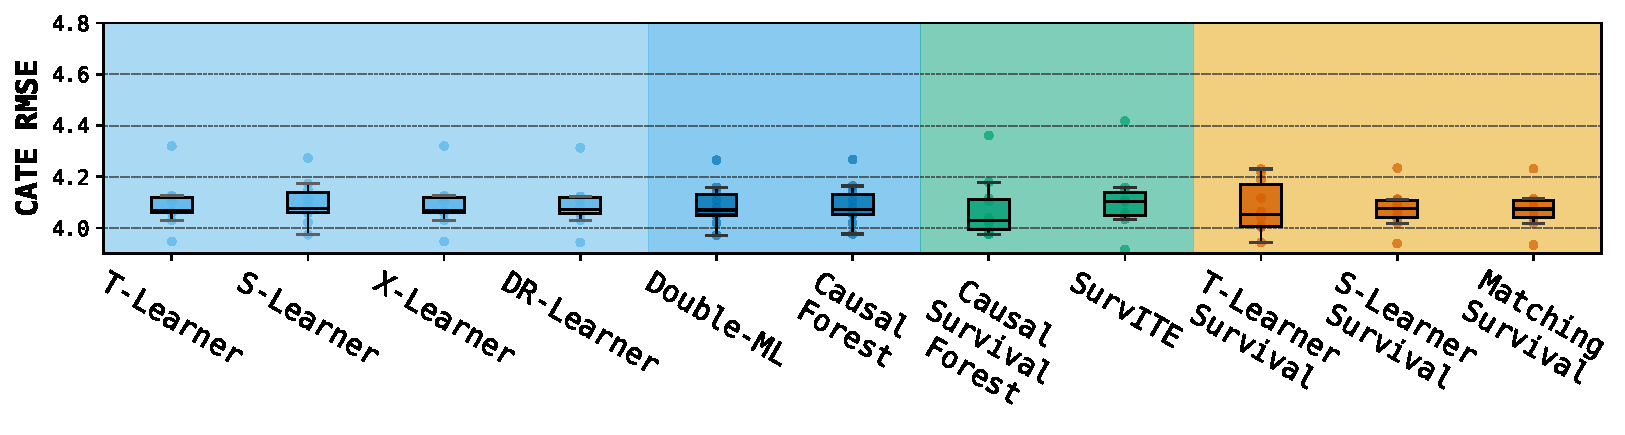
\includegraphics[width=\linewidth]{Appendices/appendix-ch04/images/figure_results_updated/cate_rmse/Scenario_E_OBS-CPS-IC_cate_mse.pdf}
        
    \end{minipage}}

    

    \subfloat[{RCT: \ChFourBlackCross, Ignorability: \ChFourBlackCross, Positivity: \ChFourGrayCheck, Ignorable Censoring: \ChFourBlackCross}]{\begin{minipage}[t]{0.49\textwidth}
        \centering
        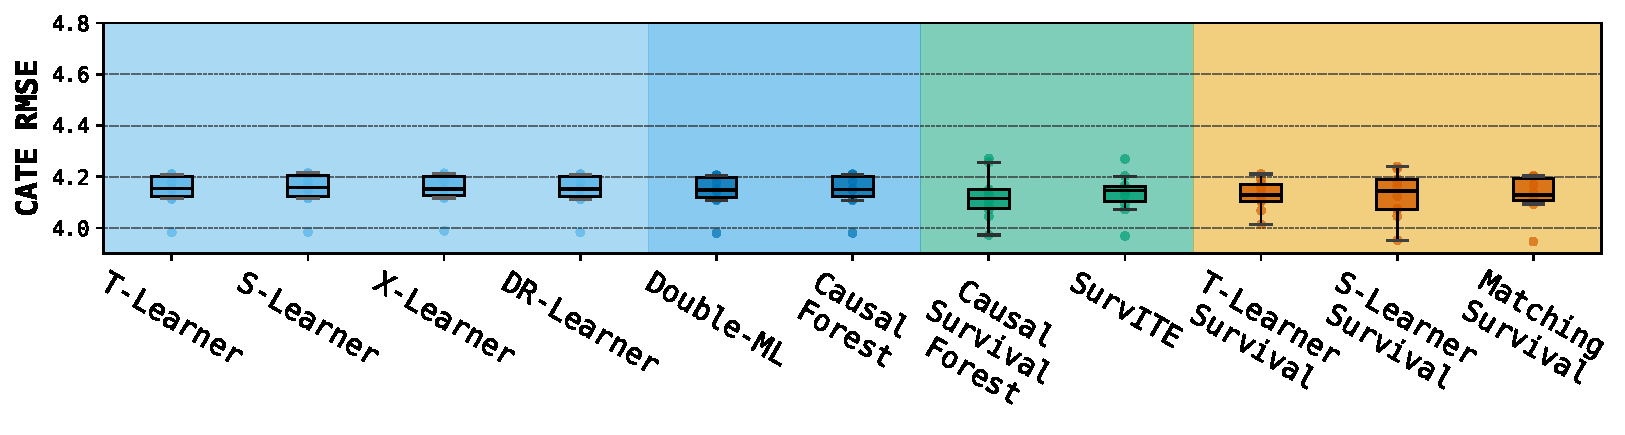
\includegraphics[width=\linewidth]{Appendices/appendix-ch04/images/figure_results_updated/cate_rmse/Scenario_E_OBS-UConf-IC_cate_mse.pdf}
        
    \end{minipage}}
    \hfill
    \subfloat[{RCT: \ChFourBlackCross, Ignorability: \ChFourGrayCheck, Positivity: \ChFourBlackCross, Ignorable Censoring: \ChFourBlackCross}]{\begin{minipage}[t]{0.49\textwidth}
        \centering
        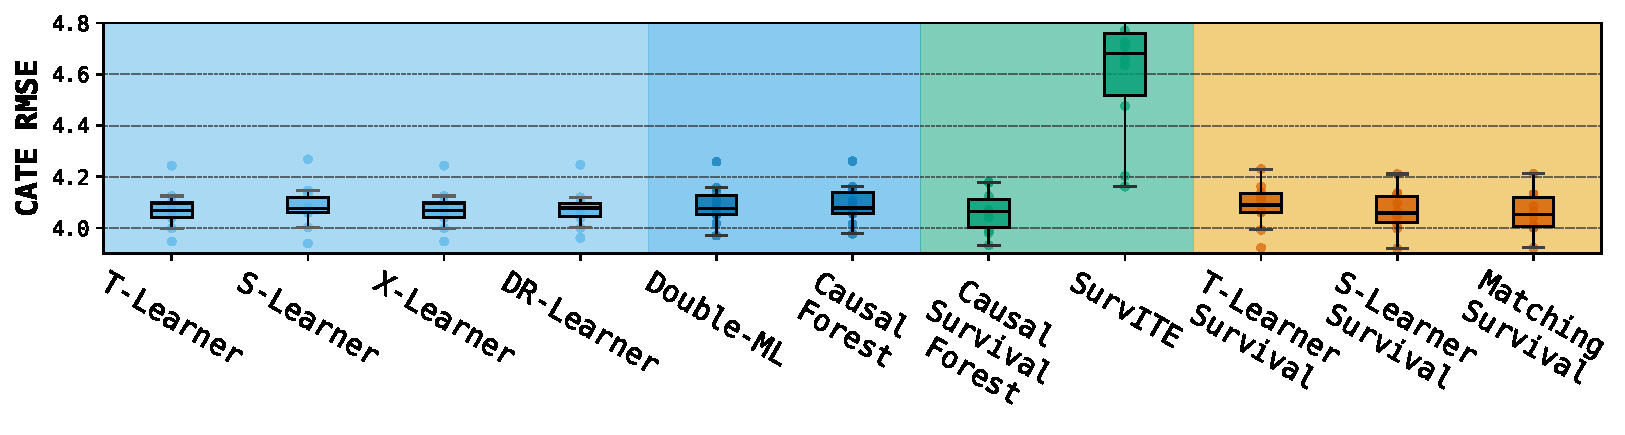
\includegraphics[width=\linewidth]{Appendices/appendix-ch04/images/figure_results_updated/cate_rmse/Scenario_E_OBS-NoPos-IC_cate_mse.pdf}
        
    \end{minipage}}

            \end{minipage}%
    }
    

    
    
}
\end{figure}






%%%%%%%%%%%%%%%%%%%%%%%%%%%%%%%%%%%%%%%%%%%%%%%%%%%%%%%%%%%%
%%%%%%%%%%%%%%%%%%%%%%%%%%%%%%%%%%%%%%%%%%%%%%%%%%%%%%%%%%%%
%%%%%%%%%%%%%%%%%%%%%%%%%%%%%%%%%%%%%%%%%%%%%%%%%%%%%%%%%%%%

\subsubsection{Figure results - ATE bias} \label{ch04:app:more-ate-plots}

This section presents the ATE bias results for each family of causal inference methods across various survival scenarios.
As with the CATE RMSE results in Appendix~\ref{ch04:app:more-cate-mse-plots}, we display performance under 8 distinct causal configurations per scenario, each varying in treatment assignment (RCT vs. observational), ignorability, positivity, and censoring assumptions.

For each survival scenario and causal configuration, the model shown corresponds to the best hyperparameter setting and base model configuration selected based on CATE RMSE performance on the validation set --- ATE bias was not used for model selection for consistent results with other sections.
The reported ATE bias values are computed on the test set and defined as the difference between the \emph{predicted ATE} from the test population and the \emph{true ATE} in the full population.

Each box plot represents results from 10 independent experimental repeats to account for random seed variability.
For meta-learners and double machine learning models, which by design can provide 95\% confidence intervals for ATE estimates, we also include these intervals in the plots---adjusted accordingly to center around the ATE bias.
These confidence intervals are obtained via 100 bootstrap samples and are notably wider than the variability observed across the 10 experimental repeats.
The zero bias line is shown as a dashed reference line.

% Secnario A

% !TeX root = ../../../main.tex
\begin{figure}[htbp]
\ChFourFloatContents{ch04:fig:ate_bias_grid_scenario_A}{\caption{ATE Bias across different experiments in Scenario \texttt{A}.}}{
    \centering

            \resizebox{0.95\textwidth}{!}{%
        \begin{minipage}{1\textwidth}

    \subfloat[{RCT: \ChFourGrayCheck (50\%), Ignorability: \ChFourGrayCheck, Positivity: \ChFourGrayCheck, Ign-Censoring: \ChFourGrayCheck}]{\begin{minipage}[t]{0.49\textwidth}
        \centering
        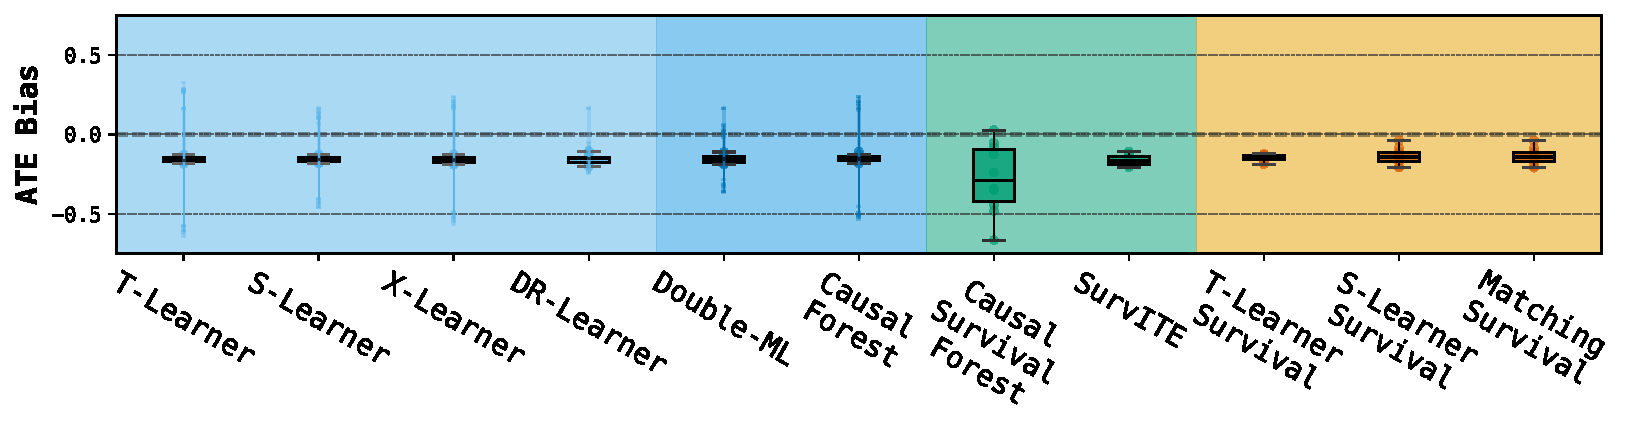
\includegraphics[width=\linewidth]{Appendices/appendix-ch04/images/figure_results_updated/ate_bias/Scenario_A_RCT-50_ate_bias.pdf}
        
    \end{minipage}}
    \hfill
    \subfloat[{RCT: \ChFourGrayCheck (5\%), Ignorability: \ChFourGrayCheck, Positivity: \ChFourGrayCheck, Ign-Censoring: \ChFourGrayCheck}]{\begin{minipage}[t]{0.49\textwidth}
        \centering
        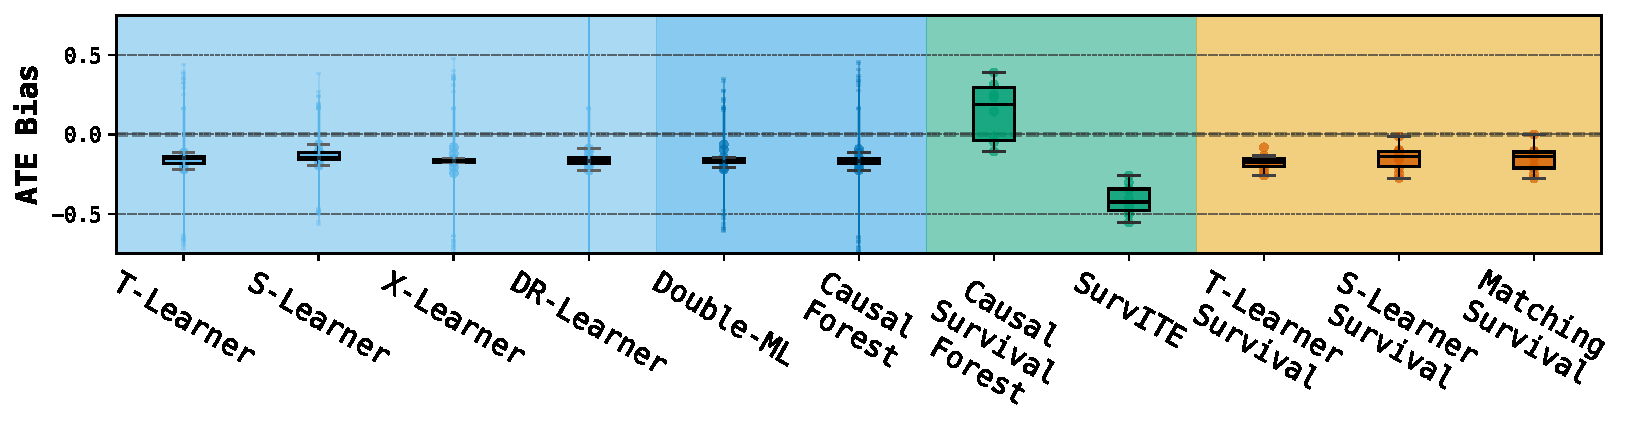
\includegraphics[width=\linewidth]{Appendices/appendix-ch04/images/figure_results_updated/ate_bias/Scenario_A_RCT-5_ate_bias.pdf}
        
    \end{minipage}}

    

    \subfloat[{RCT: \ChFourBlackCross, Ignorability: \ChFourGrayCheck, Positivity: \ChFourGrayCheck, Ignorable Censoring: \ChFourGrayCheck}]{\begin{minipage}[t]{0.49\textwidth}
        \centering
        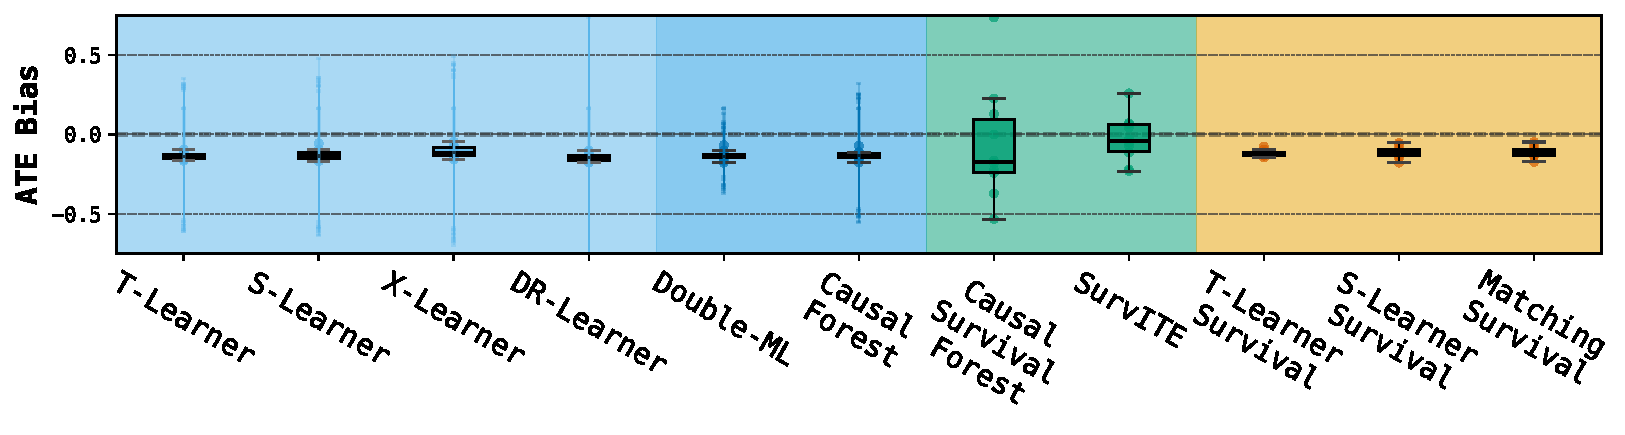
\includegraphics[width=\linewidth]{Appendices/appendix-ch04/images/figure_results_updated/ate_bias/Scenario_A_OBS-CPS_ate_bias.pdf}
        
    \end{minipage}}
    \hfill
    \subfloat[{RCT: \ChFourBlackCross, Ignorability: \ChFourBlackCross, Positivity: \ChFourGrayCheck, Ignorable Censoring: \ChFourGrayCheck}]{\begin{minipage}[t]{0.49\textwidth}
        \centering
        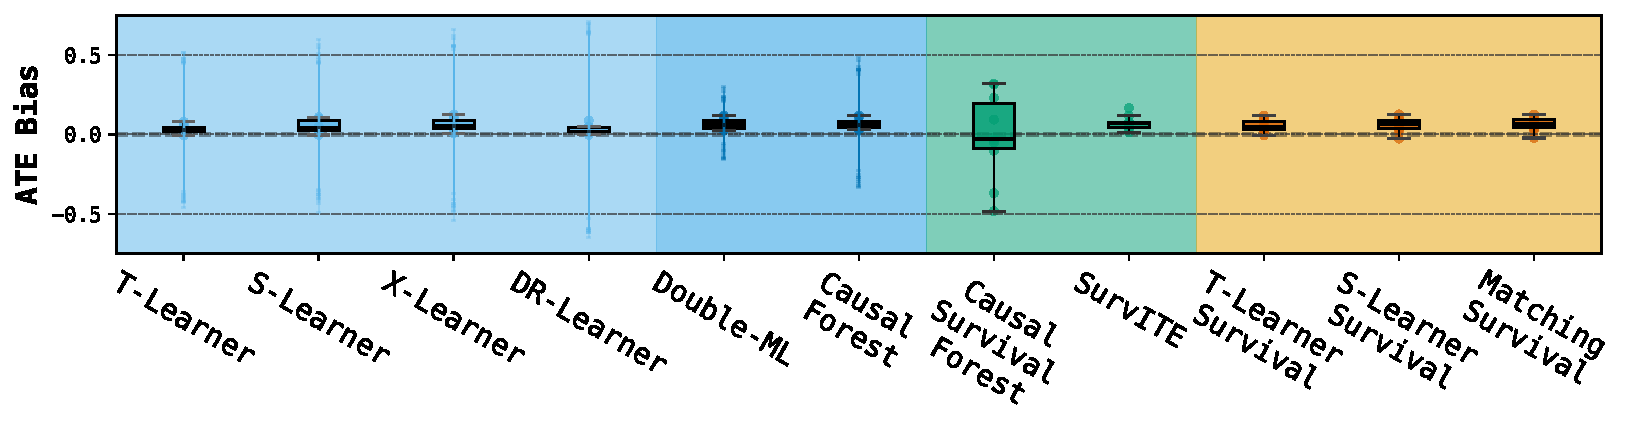
\includegraphics[width=\linewidth]{Appendices/appendix-ch04/images/figure_results_updated/ate_bias/Scenario_A_OBS-UConf_ate_bias.pdf}
        
    \end{minipage}}

    

    \subfloat[{RCT: \ChFourBlackCross, Ignorability: \ChFourGrayCheck, Positivity: \ChFourBlackCross, Ignorable Censoring: \ChFourGrayCheck}]{\begin{minipage}[t]{0.49\textwidth}
        \centering
        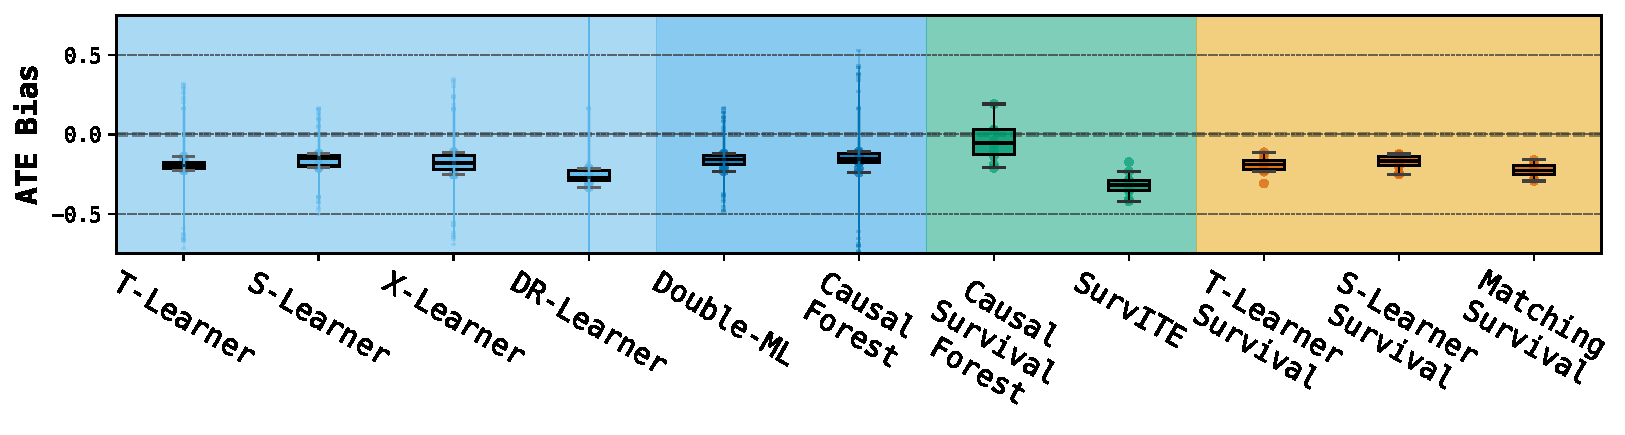
\includegraphics[width=\linewidth]{Appendices/appendix-ch04/images/figure_results_updated/ate_bias/Scenario_A_OBS-NoPos_ate_bias.pdf}
        
    \end{minipage}}
    \hfill
    \subfloat[{RCT: \ChFourBlackCross, Ignorability: \ChFourGrayCheck, Positivity: \ChFourGrayCheck, Ignorable Censoring: \ChFourBlackCross}]{\begin{minipage}[t]{0.49\textwidth}
        \centering
        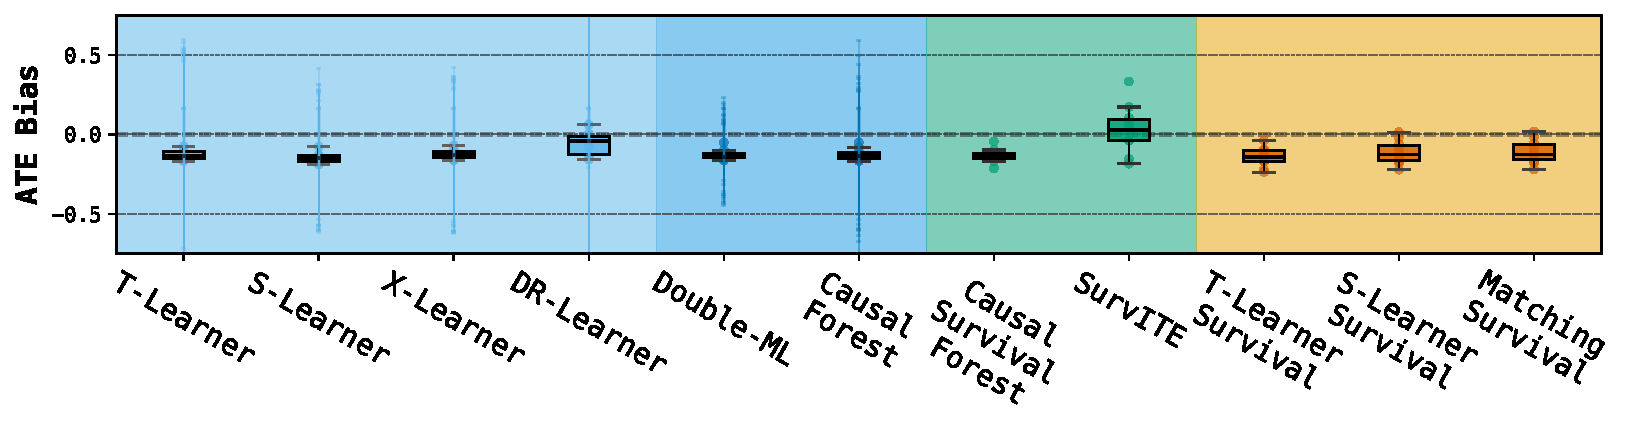
\includegraphics[width=\linewidth]{Appendices/appendix-ch04/images/figure_results_updated/ate_bias/Scenario_A_OBS-CPS-IC_ate_bias.pdf}
        
    \end{minipage}}

    

    \subfloat[{RCT: \ChFourBlackCross, Ignorability: \ChFourBlackCross, Positivity: \ChFourGrayCheck, Ignorable Censoring: \ChFourBlackCross}]{\begin{minipage}[t]{0.49\textwidth}
        \centering
        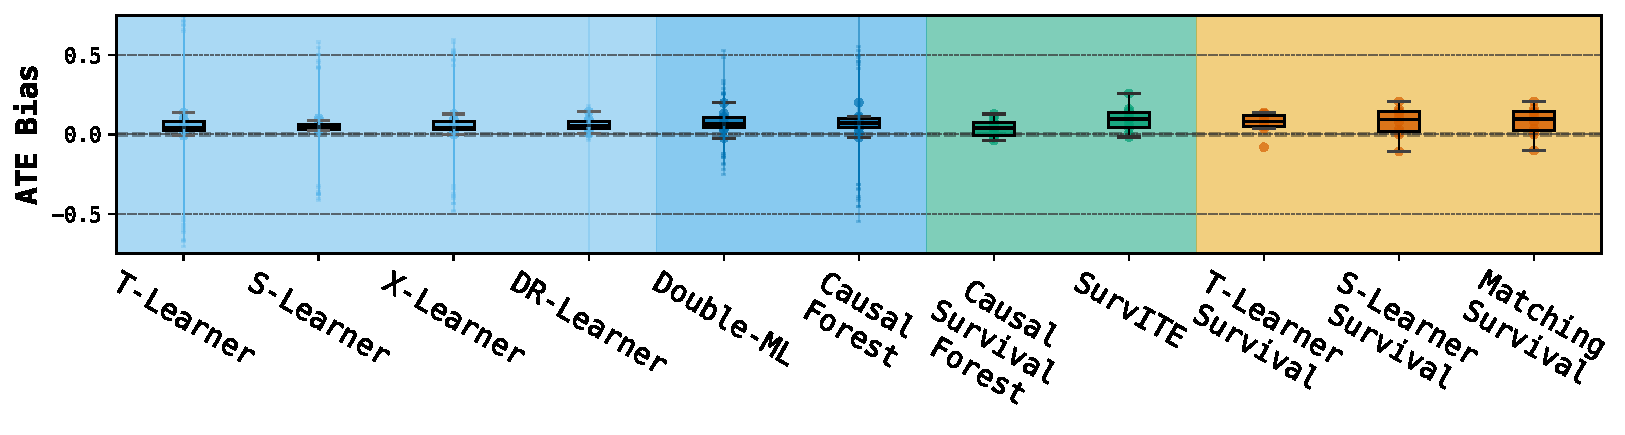
\includegraphics[width=\linewidth]{Appendices/appendix-ch04/images/figure_results_updated/ate_bias/Scenario_A_OBS-UConf-IC_ate_bias.pdf}
        
    \end{minipage}}
    \hfill
    \subfloat[{RCT: \ChFourBlackCross, Ignorability: \ChFourGrayCheck, Positivity: \ChFourBlackCross, Ignorable Censoring: \ChFourBlackCross}]{\begin{minipage}[t]{0.49\textwidth}
        \centering
        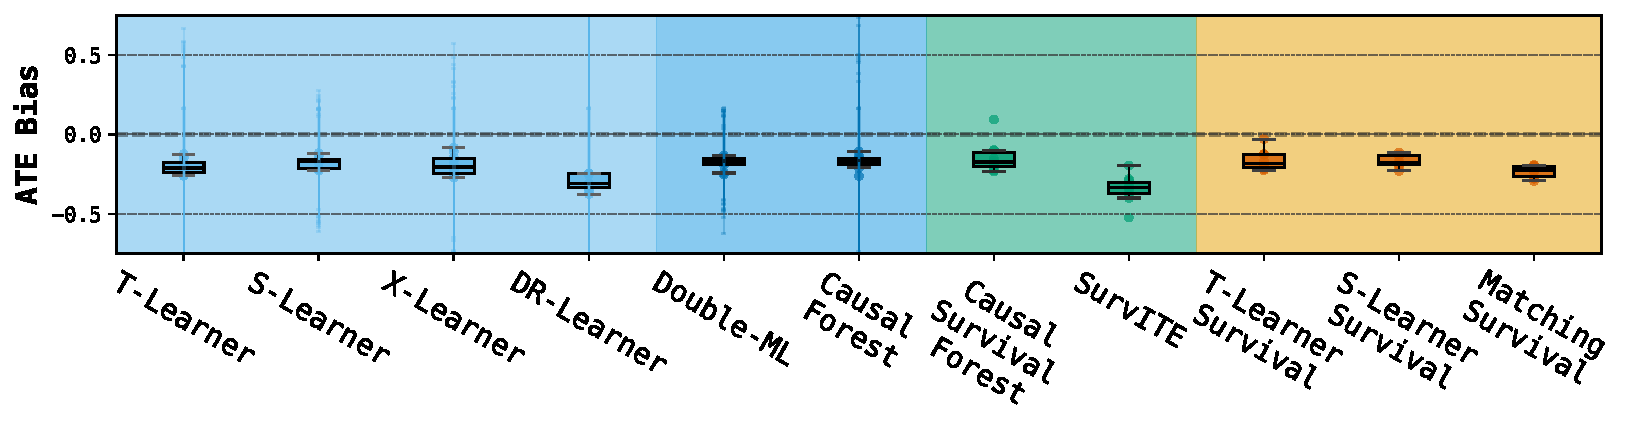
\includegraphics[width=\linewidth]{Appendices/appendix-ch04/images/figure_results_updated/ate_bias/Scenario_A_OBS-NoPos-IC_ate_bias.pdf}
        
    \end{minipage}}

                    \end{minipage}%
    }

    
    
}
\end{figure}

% 



% Secnario B

% !TeX root = ../../../main.tex
\begin{figure}[htbp]
\ChFourFloatContents{ch04:fig:ate_bias_grid_scenario_B}{\caption{ATE Bias across different experiments in Scenario \texttt{B}.}}{
    \centering

            \resizebox{0.95\textwidth}{!}{%
        \begin{minipage}{1\textwidth}

    \subfloat[{RCT: \ChFourGrayCheck (50\%), Ignorability: \ChFourGrayCheck, Positivity: \ChFourGrayCheck, Ign-Censoring: \ChFourGrayCheck}]{\begin{minipage}[t]{0.49\textwidth}
        \centering
        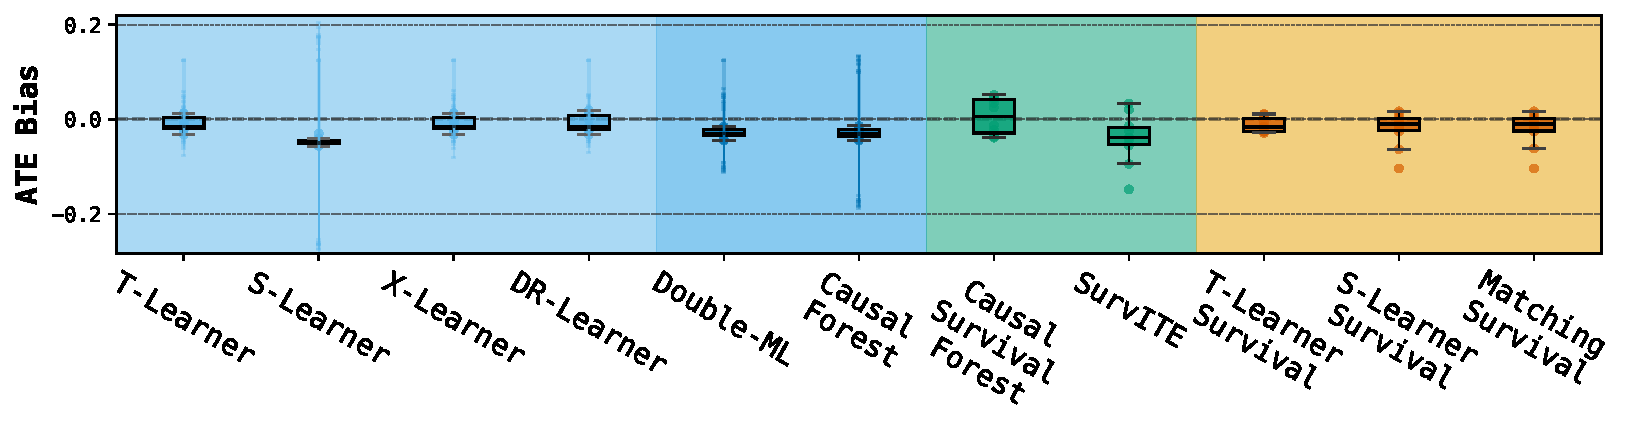
\includegraphics[width=\linewidth]{Appendices/appendix-ch04/images/figure_results_updated/ate_bias/Scenario_B_RCT-50_ate_bias.pdf}
        
    \end{minipage}}
    \hfill
    \subfloat[{RCT: \ChFourGrayCheck (5\%), Ignorability: \ChFourGrayCheck, Positivity: \ChFourGrayCheck, Ign-Censoring: \ChFourGrayCheck}]{\begin{minipage}[t]{0.49\textwidth}
        \centering
        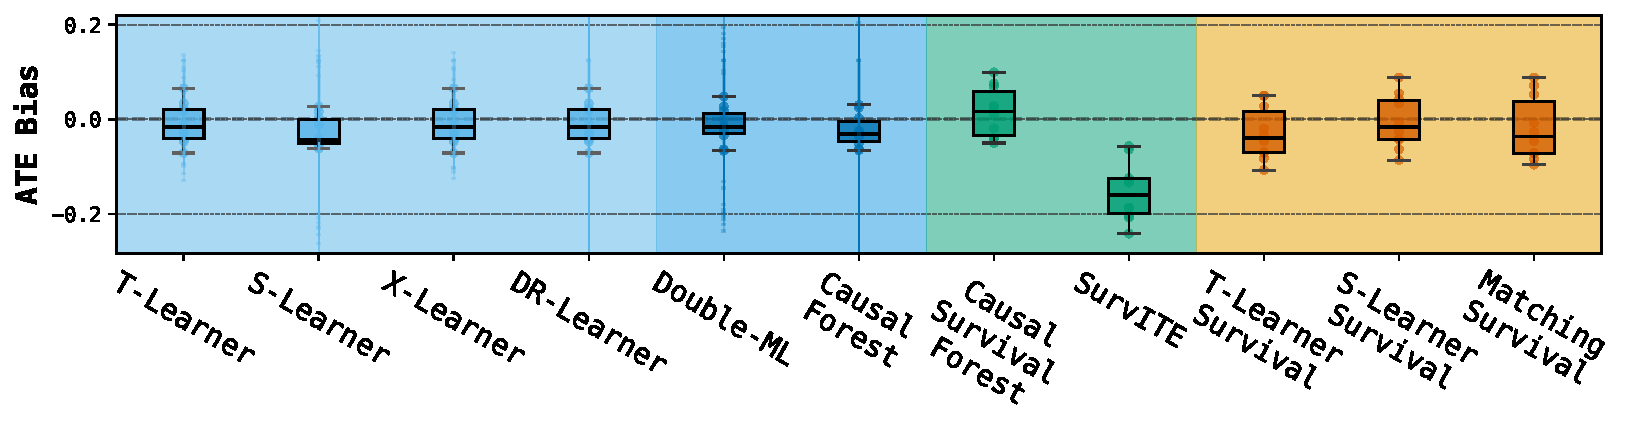
\includegraphics[width=\linewidth]{Appendices/appendix-ch04/images/figure_results_updated/ate_bias/Scenario_B_RCT-5_ate_bias.pdf}
        
    \end{minipage}}

    

    \subfloat[{RCT: \ChFourBlackCross, Ignorability: \ChFourGrayCheck, Positivity: \ChFourGrayCheck, Ignorable Censoring: \ChFourGrayCheck}]{\begin{minipage}[t]{0.49\textwidth}
        \centering
        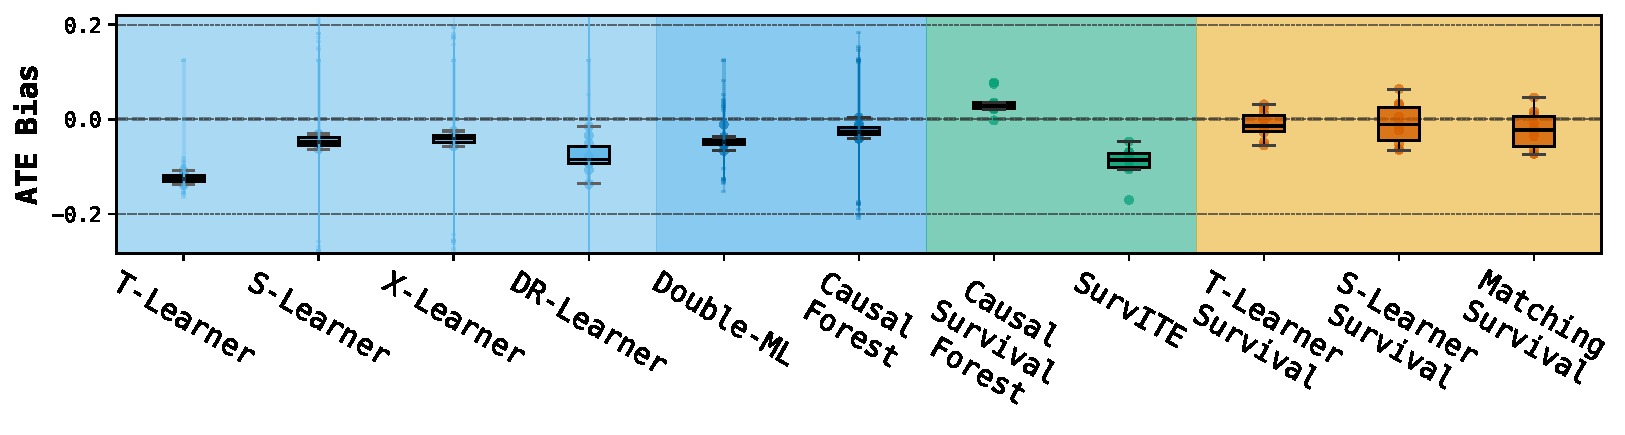
\includegraphics[width=\linewidth]{Appendices/appendix-ch04/images/figure_results_updated/ate_bias/Scenario_B_OBS-CPS_ate_bias.pdf}
        
    \end{minipage}}
    \hfill
    \subfloat[{RCT: \ChFourBlackCross, Ignorability: \ChFourBlackCross, Positivity: \ChFourGrayCheck, Ignorable Censoring: \ChFourGrayCheck}]{\begin{minipage}[t]{0.49\textwidth}
        \centering
        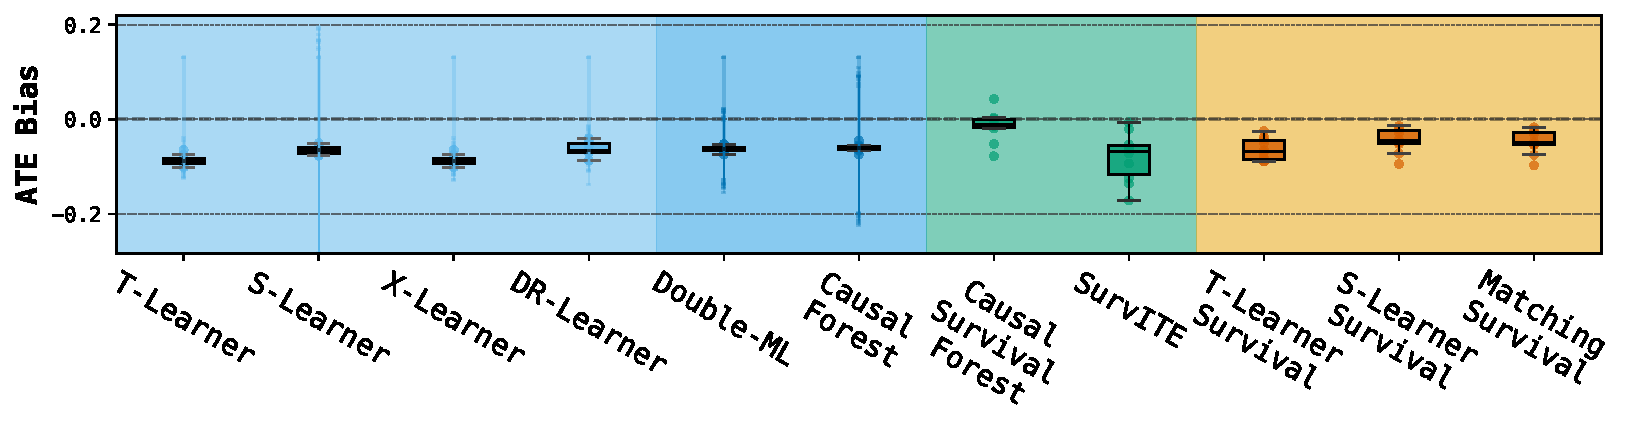
\includegraphics[width=\linewidth]{Appendices/appendix-ch04/images/figure_results_updated/ate_bias/Scenario_B_OBS-UConf_ate_bias.pdf}
        
    \end{minipage}}

    

    \subfloat[{RCT: \ChFourBlackCross, Ignorability: \ChFourGrayCheck, Positivity: \ChFourBlackCross, Ignorable Censoring: \ChFourGrayCheck}]{\begin{minipage}[t]{0.49\textwidth}
        \centering
        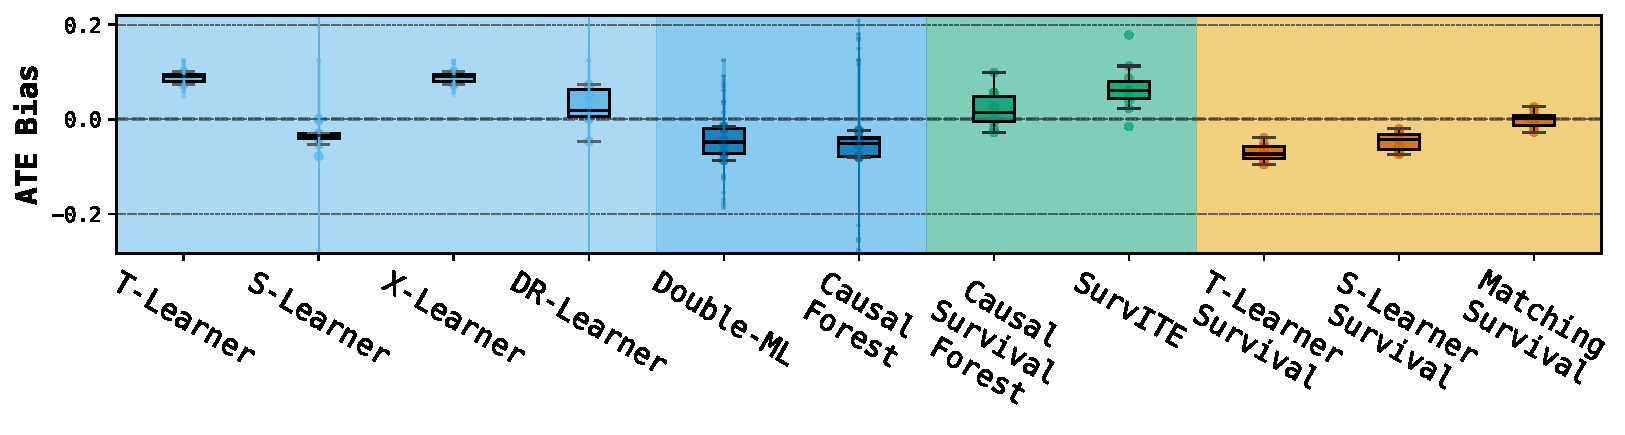
\includegraphics[width=\linewidth]{Appendices/appendix-ch04/images/figure_results_updated/ate_bias/Scenario_B_OBS-NoPos_ate_bias.pdf}
        
    \end{minipage}}
    \hfill
    \subfloat[{RCT: \ChFourBlackCross, Ignorability: \ChFourGrayCheck, Positivity: \ChFourGrayCheck, Ignorable Censoring: \ChFourBlackCross}]{\begin{minipage}[t]{0.49\textwidth}
        \centering
        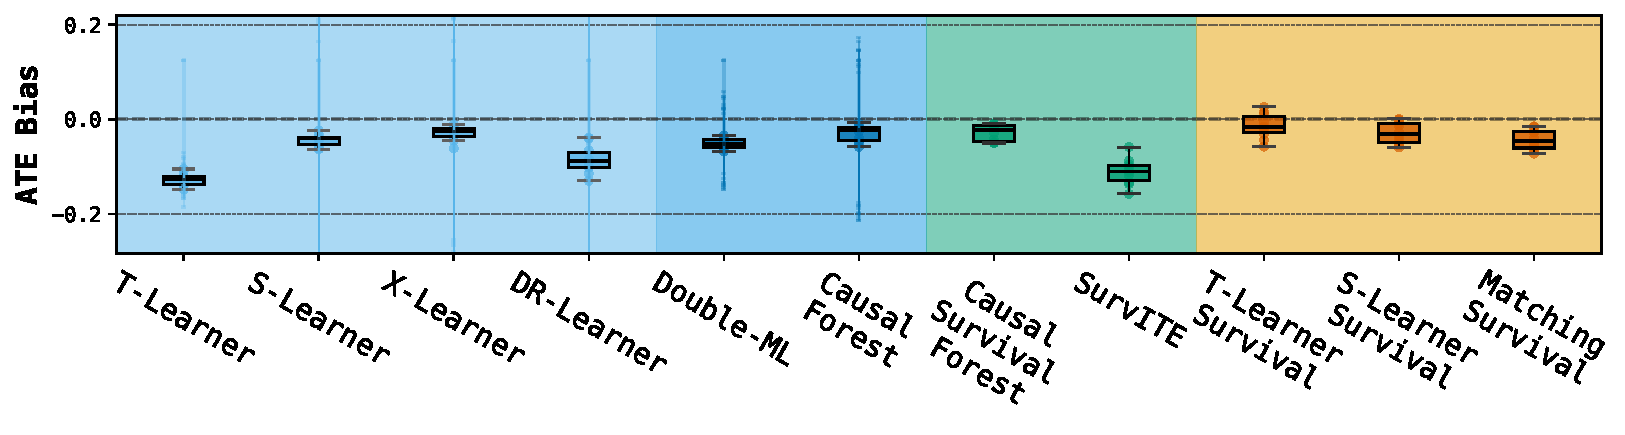
\includegraphics[width=\linewidth]{Appendices/appendix-ch04/images/figure_results_updated/ate_bias/Scenario_B_OBS-CPS-IC_ate_bias.pdf}
        
    \end{minipage}}

    

    \subfloat[{RCT: \ChFourBlackCross, Ignorability: \ChFourBlackCross, Positivity: \ChFourGrayCheck, Ignorable Censoring: \ChFourBlackCross}]{\begin{minipage}[t]{0.49\textwidth}
        \centering
        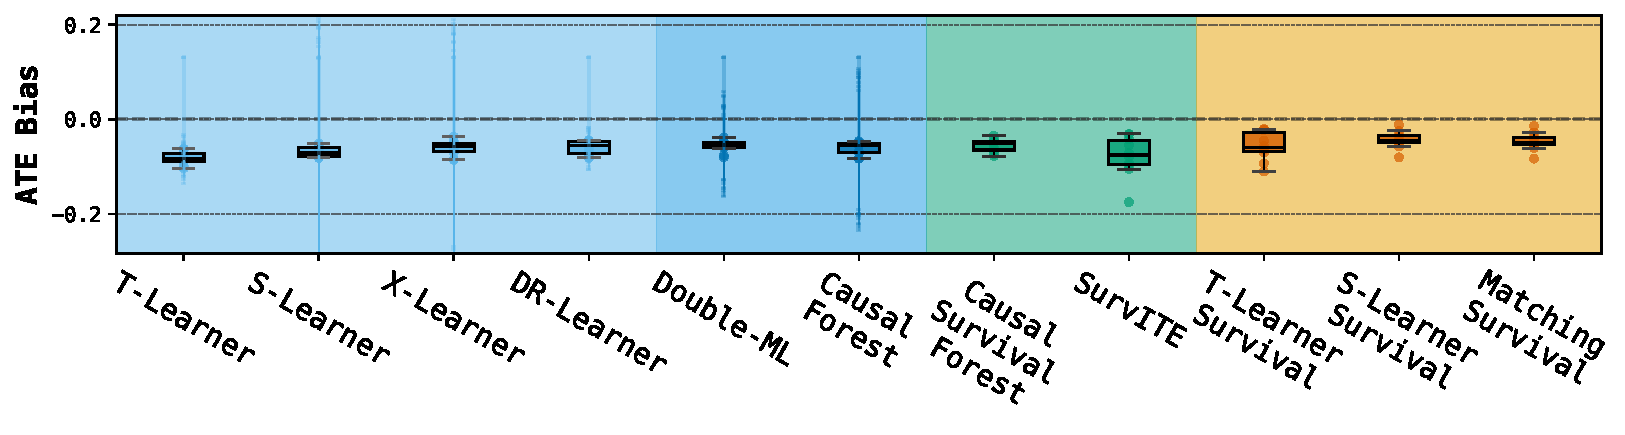
\includegraphics[width=\linewidth]{Appendices/appendix-ch04/images/figure_results_updated/ate_bias/Scenario_B_OBS-UConf-IC_ate_bias.pdf}
        
    \end{minipage}}
    \hfill
    \subfloat[{RCT: \ChFourBlackCross, Ignorability: \ChFourGrayCheck, Positivity: \ChFourBlackCross, Ignorable Censoring: \ChFourBlackCross}]{\begin{minipage}[t]{0.49\textwidth}
        \centering
        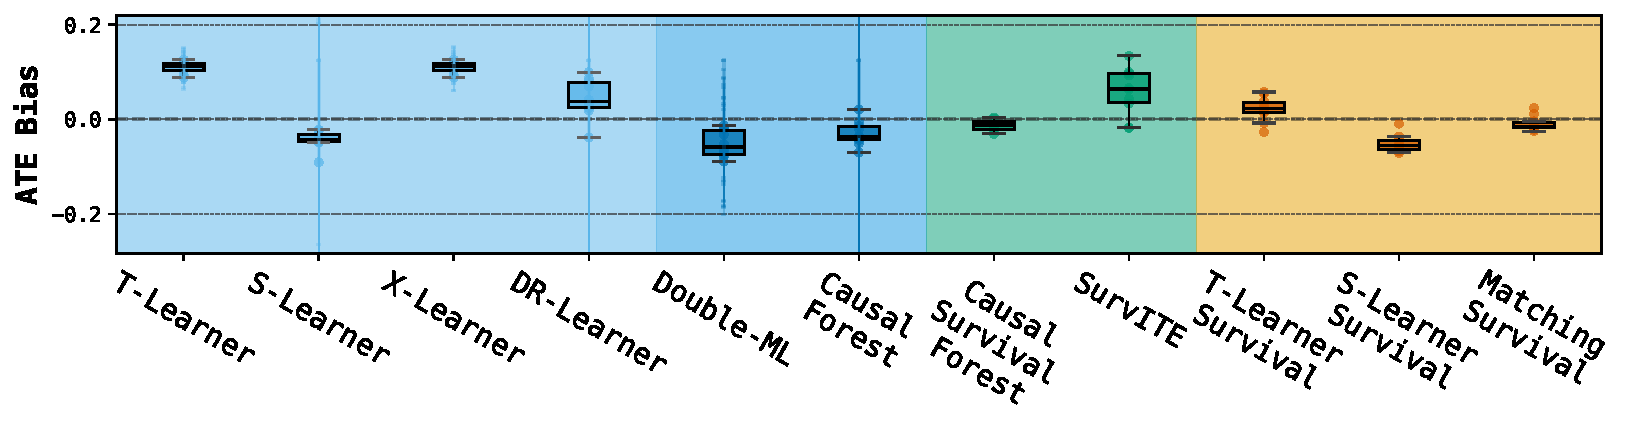
\includegraphics[width=\linewidth]{Appendices/appendix-ch04/images/figure_results_updated/ate_bias/Scenario_B_OBS-NoPos-IC_ate_bias.pdf}
        
    \end{minipage}}

                    \end{minipage}%
    }

    
    
}
\end{figure}


% 

% Secnario C

% !TeX root = ../../../main.tex
\begin{figure}[htbp]
\ChFourFloatContents{ch04:fig:ate_bias_grid_scenario_C}{\caption{ATE Bias across different experiments in Scenario \texttt{C}.}}{
    \centering

            \resizebox{0.95\textwidth}{!}{%
        \begin{minipage}{1\textwidth}

    \subfloat[{RCT: \ChFourGrayCheck (50\%), Ignorability: \ChFourGrayCheck, Positivity: \ChFourGrayCheck, Ign-Censoring: \ChFourGrayCheck}]{\begin{minipage}[t]{0.49\textwidth}
        \centering
        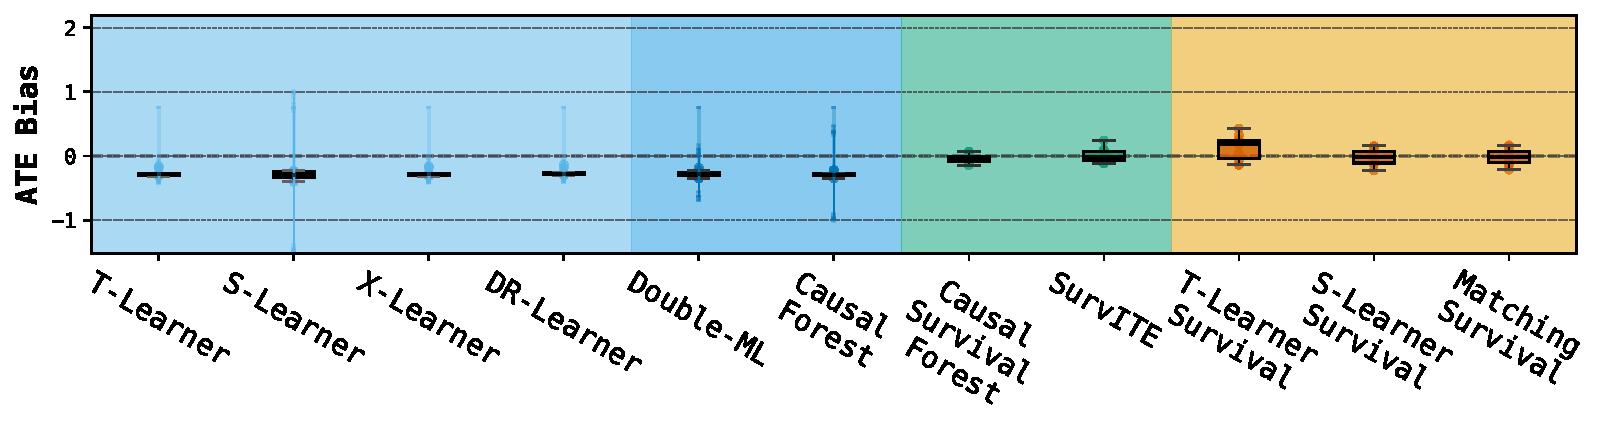
\includegraphics[width=\linewidth]{Appendices/appendix-ch04/images/figure_results_updated/ate_bias/Scenario_C_RCT-50_ate_bias.pdf}
        
    \end{minipage}}
    \hfill
    \subfloat[{RCT: \ChFourGrayCheck (5\%), Ignorability: \ChFourGrayCheck, Positivity: \ChFourGrayCheck, Ign-Censoring: \ChFourGrayCheck}]{\begin{minipage}[t]{0.49\textwidth}
        \centering
        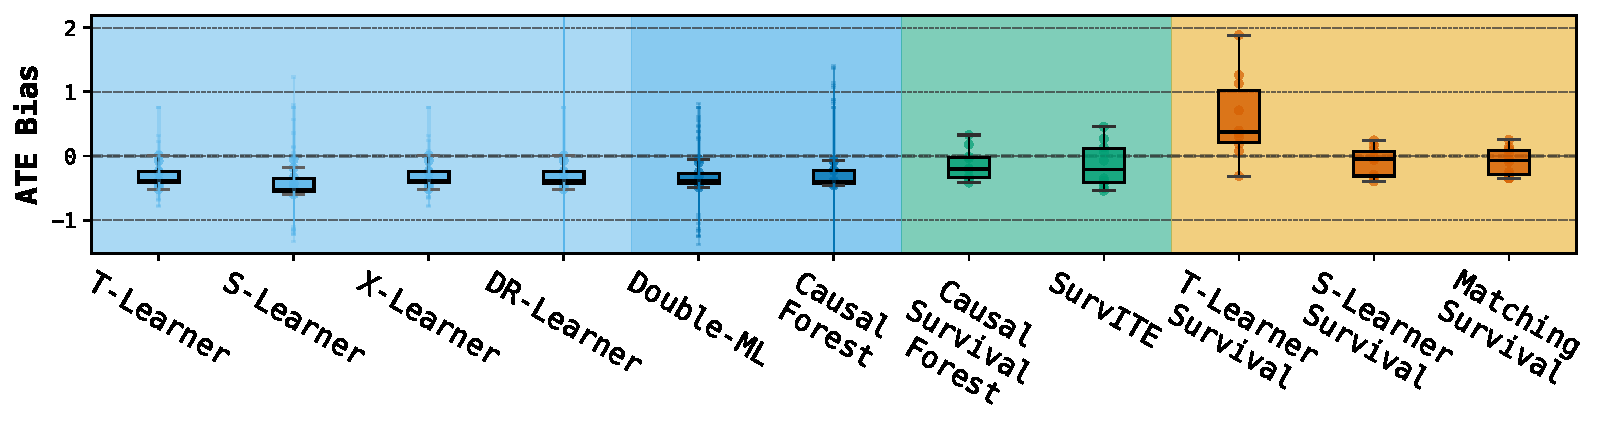
\includegraphics[width=\linewidth]{Appendices/appendix-ch04/images/figure_results_updated/ate_bias/Scenario_C_RCT-5_ate_bias.pdf}
        
    \end{minipage}}

    

    \subfloat[{RCT: \ChFourBlackCross, Ignorability: \ChFourGrayCheck, Positivity: \ChFourGrayCheck, Ignorable Censoring: \ChFourGrayCheck}]{\begin{minipage}[t]{0.49\textwidth}
        \centering
        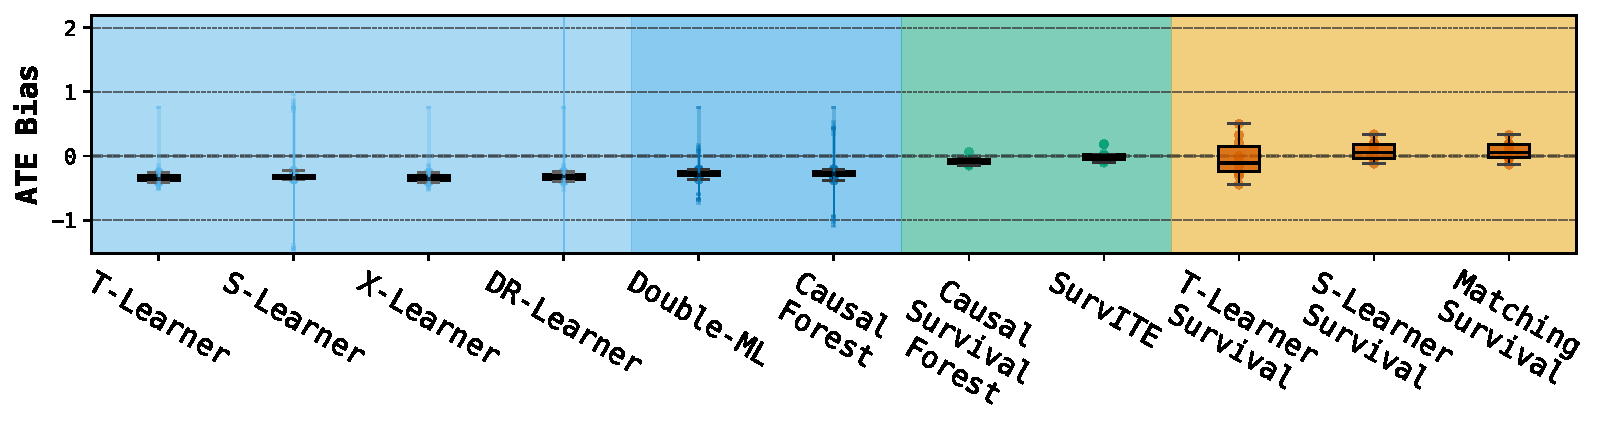
\includegraphics[width=\linewidth]{Appendices/appendix-ch04/images/figure_results_updated/ate_bias/Scenario_C_OBS-CPS_ate_bias.pdf}
        
    \end{minipage}}
    \hfill
    \subfloat[{RCT: \ChFourBlackCross, Ignorability: \ChFourBlackCross, Positivity: \ChFourGrayCheck, Ignorable Censoring: \ChFourGrayCheck}]{\begin{minipage}[t]{0.49\textwidth}
        \centering
        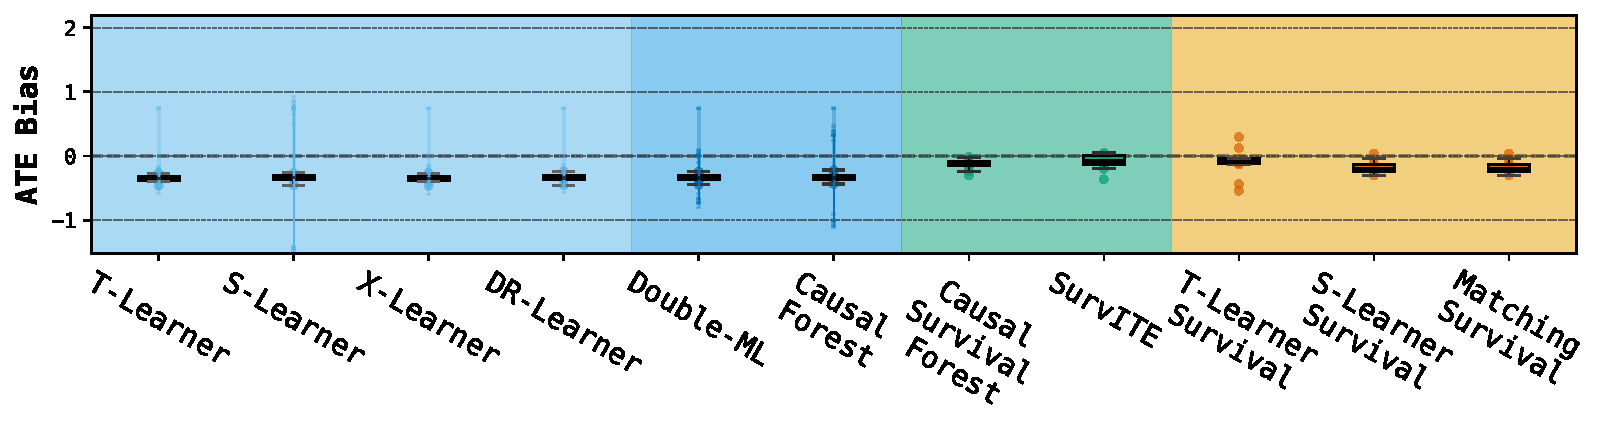
\includegraphics[width=\linewidth]{Appendices/appendix-ch04/images/figure_results_updated/ate_bias/Scenario_C_OBS-UConf_ate_bias.pdf}
        
    \end{minipage}}

    

    \subfloat[{RCT: \ChFourBlackCross, Ignorability: \ChFourGrayCheck, Positivity: \ChFourBlackCross, Ignorable Censoring: \ChFourGrayCheck}]{\begin{minipage}[t]{0.49\textwidth}
        \centering
        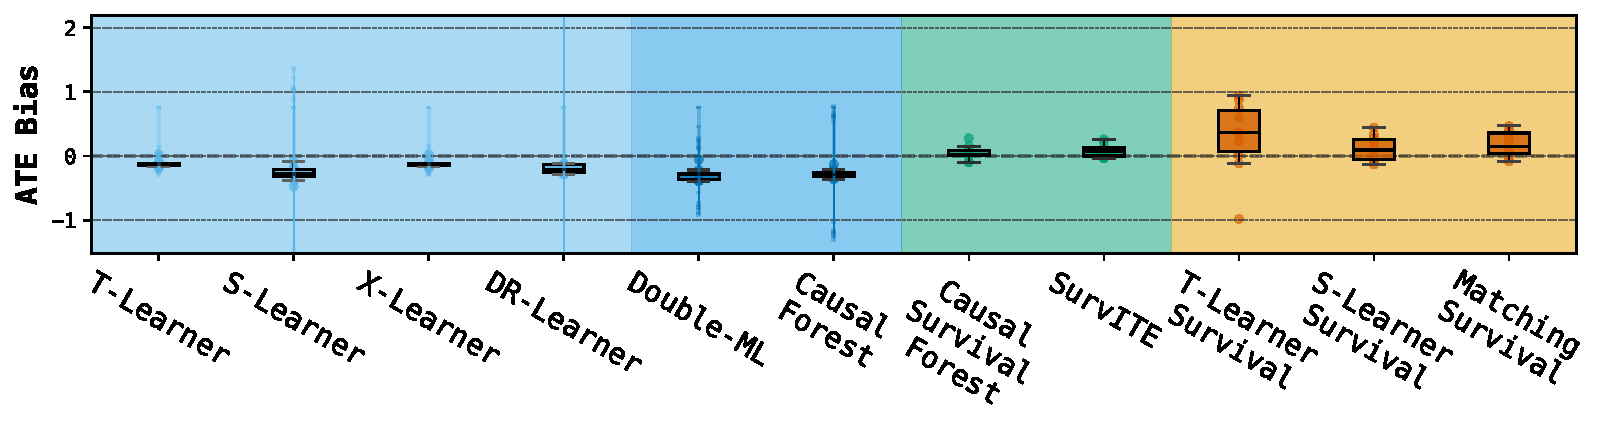
\includegraphics[width=\linewidth]{Appendices/appendix-ch04/images/figure_results_updated/ate_bias/Scenario_C_OBS-NoPos_ate_bias.pdf}
        
    \end{minipage}}
    \hfill
    \subfloat[{RCT: \ChFourBlackCross, Ignorability: \ChFourGrayCheck, Positivity: \ChFourGrayCheck, Ignorable Censoring: \ChFourBlackCross}]{\begin{minipage}[t]{0.49\textwidth}
        \centering
        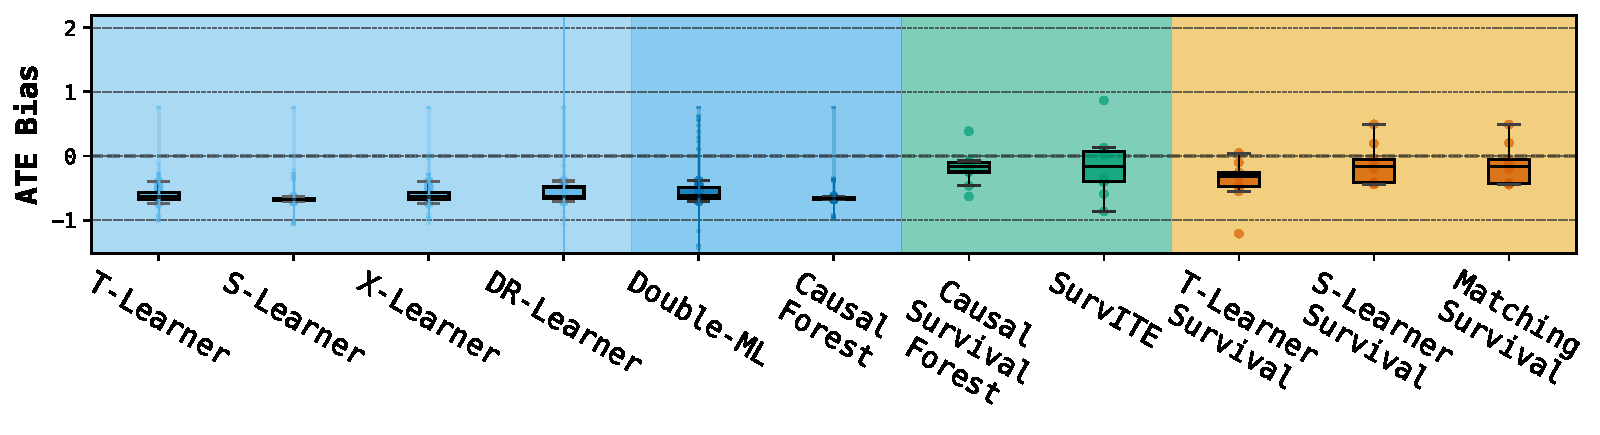
\includegraphics[width=\linewidth]{Appendices/appendix-ch04/images/figure_results_updated/ate_bias/Scenario_C_OBS-CPS-IC_ate_bias.pdf}
        
    \end{minipage}}

    

    \subfloat[{RCT: \ChFourBlackCross, Ignorability: \ChFourBlackCross, Positivity: \ChFourGrayCheck, Ignorable Censoring: \ChFourBlackCross}]{\begin{minipage}[t]{0.49\textwidth}
        \centering
        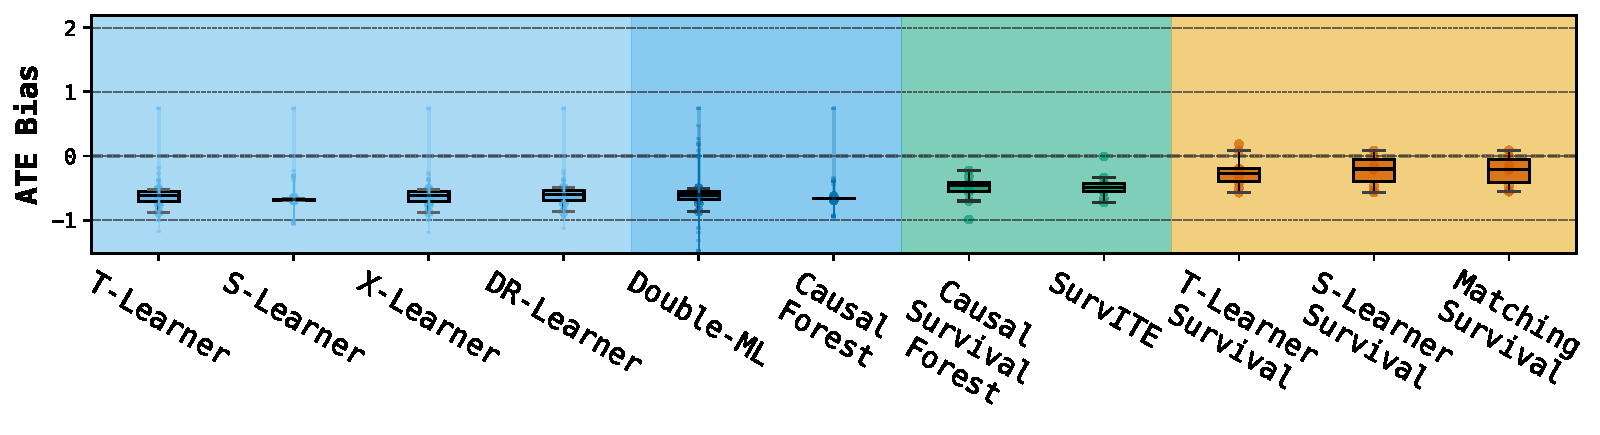
\includegraphics[width=\linewidth]{Appendices/appendix-ch04/images/figure_results_updated/ate_bias/Scenario_C_OBS-UConf-IC_ate_bias.pdf}
        
    \end{minipage}}
    \hfill
    \subfloat[{RCT: \ChFourBlackCross, Ignorability: \ChFourGrayCheck, Positivity: \ChFourBlackCross, Ignorable Censoring: \ChFourBlackCross}]{\begin{minipage}[t]{0.49\textwidth}
        \centering
        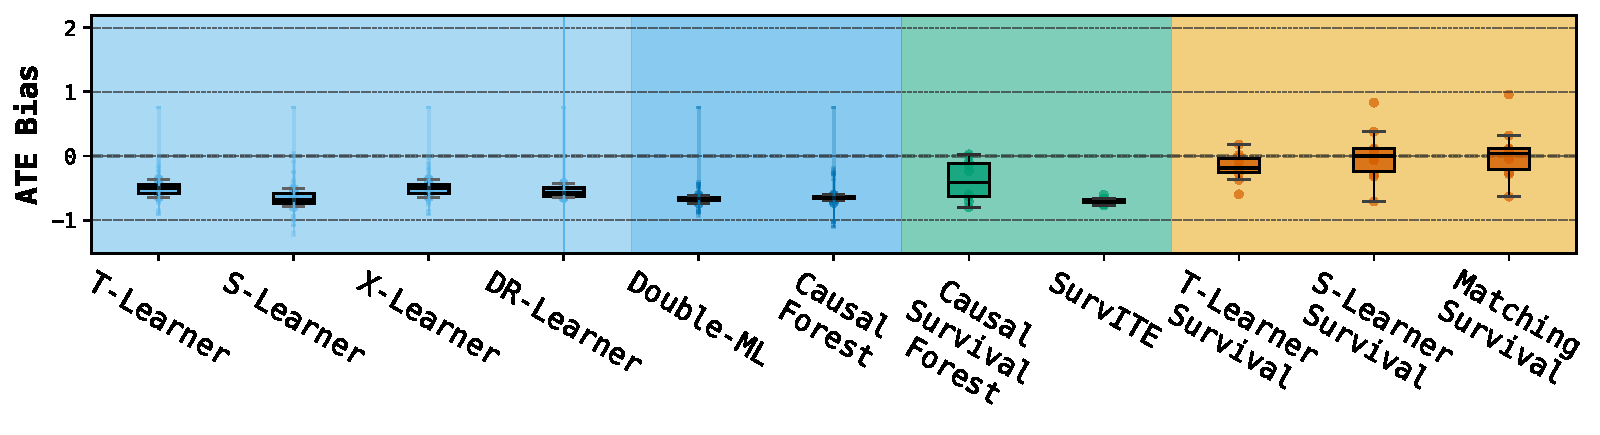
\includegraphics[width=\linewidth]{Appendices/appendix-ch04/images/figure_results_updated/ate_bias/Scenario_C_OBS-NoPos-IC_ate_bias.pdf}
        
    \end{minipage}}

                    \end{minipage}%
    }

    
    
}
\end{figure}


% 



% Scenario D

% !TeX root = ../../../main.tex
\begin{figure}[htbp]
\ChFourFloatContents{ch04:fig:ate_bias_grid_scenario_D}{\caption{ATE Bias across different experiments in Scenario \texttt{D}.}}{
    \centering

            \resizebox{0.95\textwidth}{!}{%
        \begin{minipage}{1\textwidth}

    \subfloat[{RCT: \ChFourGrayCheck (50\%), Ignorability: \ChFourGrayCheck, Positivity: \ChFourGrayCheck, Ign-Censoring: \ChFourGrayCheck}]{\begin{minipage}[t]{0.49\textwidth}
        \centering
        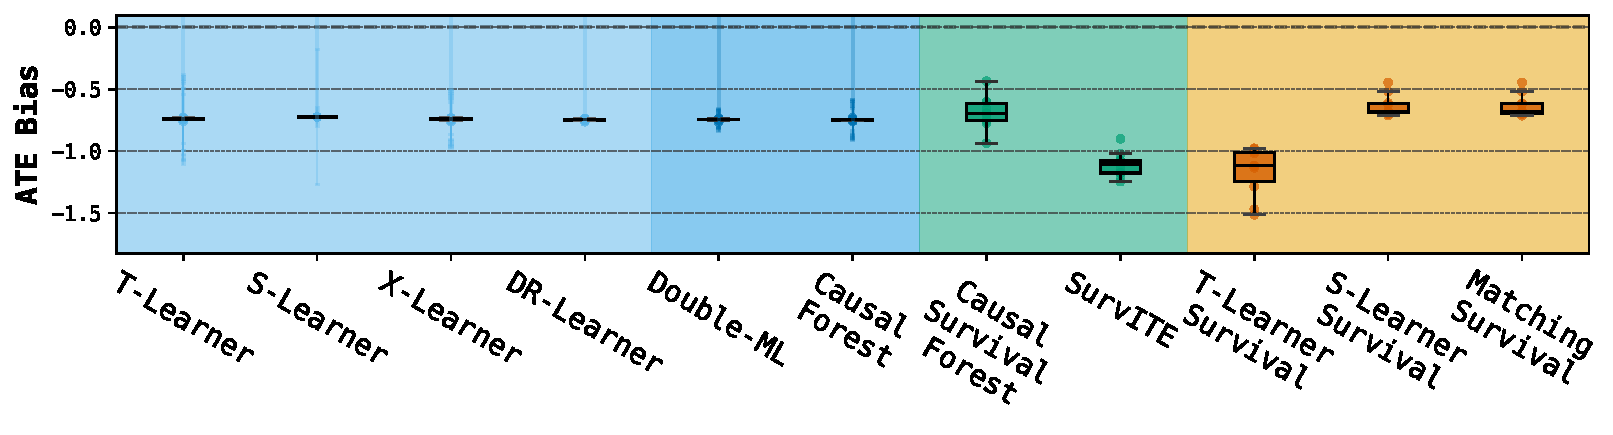
\includegraphics[width=\linewidth]{Appendices/appendix-ch04/images/figure_results_updated/ate_bias/Scenario_D_RCT-50_ate_bias.pdf}
        
    \end{minipage}}
    \hfill
    \subfloat[{RCT: \ChFourGrayCheck (5\%), Ignorability: \ChFourGrayCheck, Positivity: \ChFourGrayCheck, Ign-Censoring: \ChFourGrayCheck}]{\begin{minipage}[t]{0.49\textwidth}
        \centering
        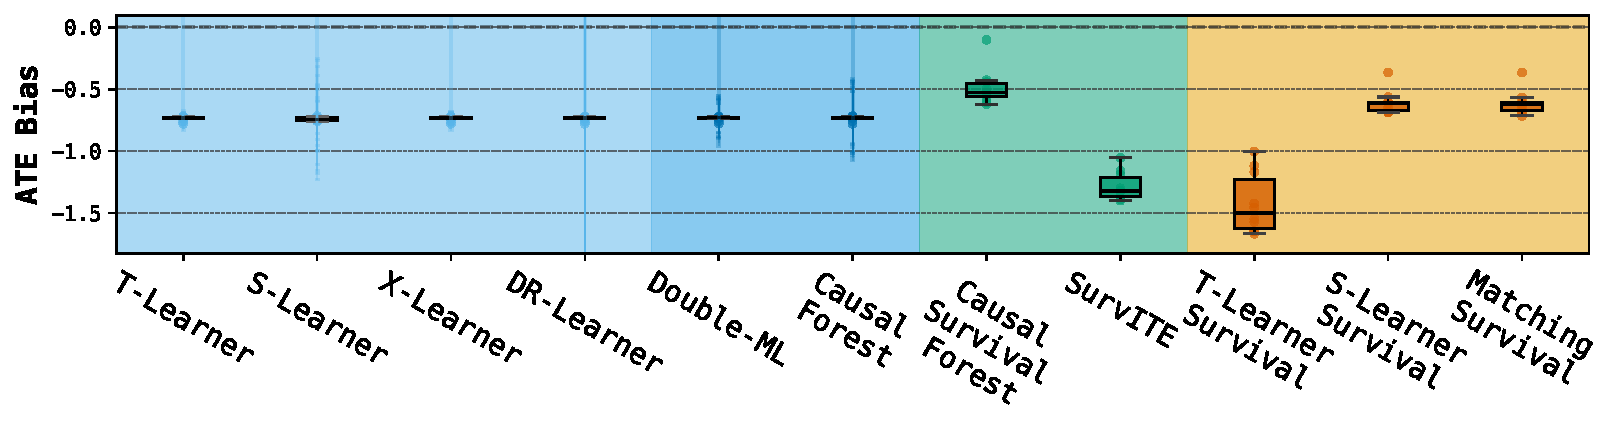
\includegraphics[width=\linewidth]{Appendices/appendix-ch04/images/figure_results_updated/ate_bias/Scenario_D_RCT-5_ate_bias.pdf}
        
    \end{minipage}}

    

    \subfloat[{RCT: \ChFourBlackCross, Ignorability: \ChFourGrayCheck, Positivity: \ChFourGrayCheck, Ignorable Censoring: \ChFourGrayCheck}]{\begin{minipage}[t]{0.49\textwidth}
        \centering
        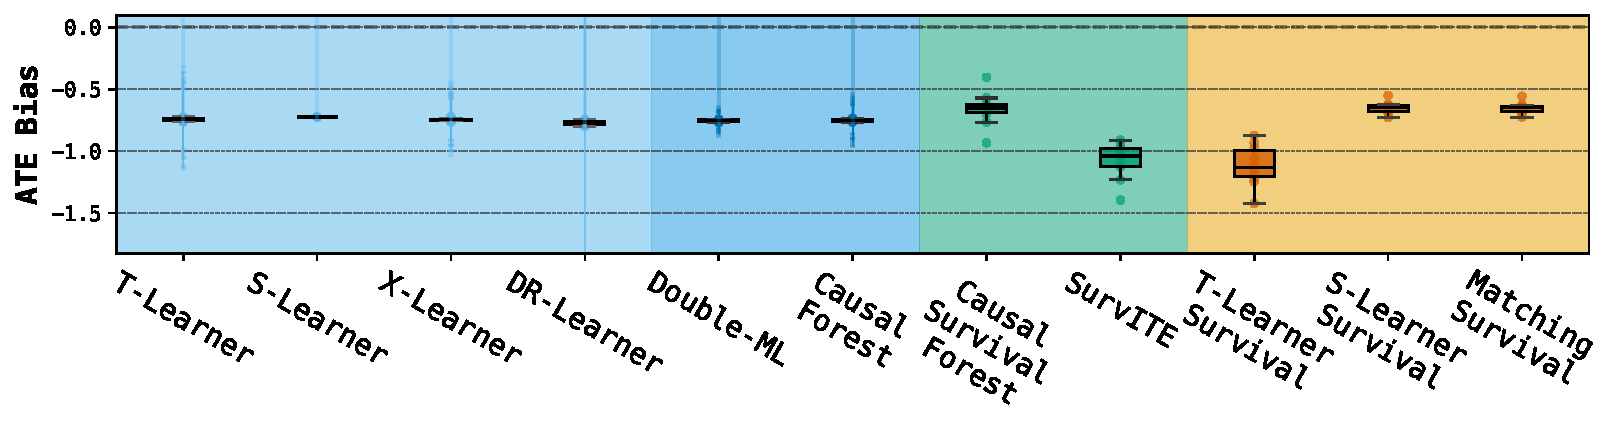
\includegraphics[width=\linewidth]{Appendices/appendix-ch04/images/figure_results_updated/ate_bias/Scenario_D_OBS-CPS_ate_bias.pdf}
        
    \end{minipage}}
    \hfill
    \subfloat[{RCT: \ChFourBlackCross, Ignorability: \ChFourBlackCross, Positivity: \ChFourGrayCheck, Ignorable Censoring: \ChFourGrayCheck}]{\begin{minipage}[t]{0.49\textwidth}
        \centering
        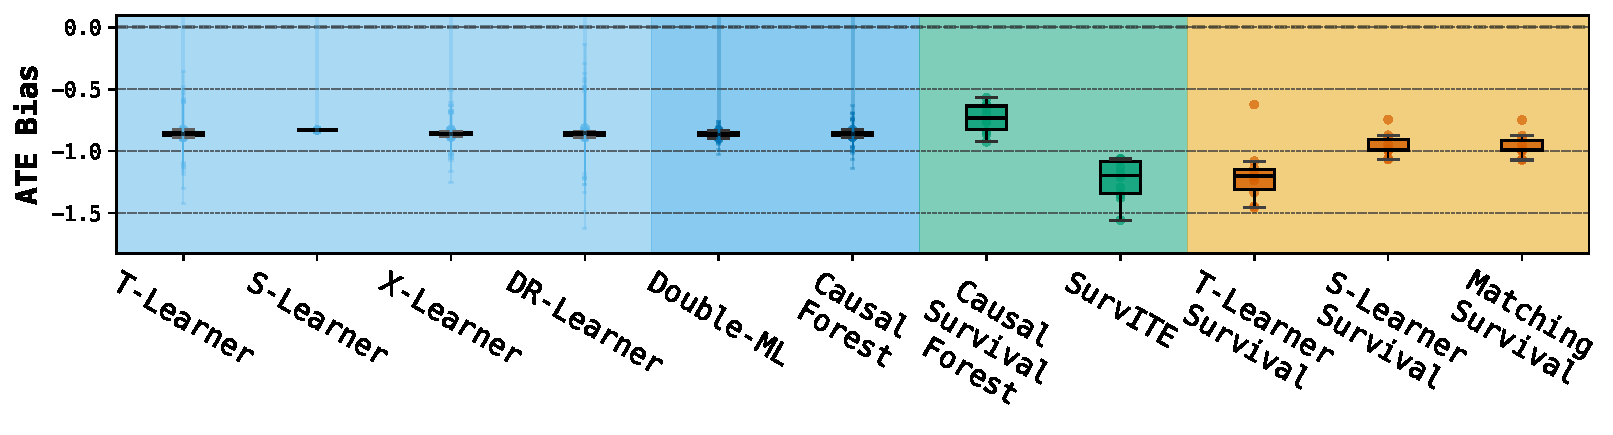
\includegraphics[width=\linewidth]{Appendices/appendix-ch04/images/figure_results_updated/ate_bias/Scenario_D_OBS-UConf_ate_bias.pdf}
        
    \end{minipage}}

    

    \subfloat[{RCT: \ChFourBlackCross, Ignorability: \ChFourGrayCheck, Positivity: \ChFourBlackCross, Ignorable Censoring: \ChFourGrayCheck}]{\begin{minipage}[t]{0.49\textwidth}
        \centering
        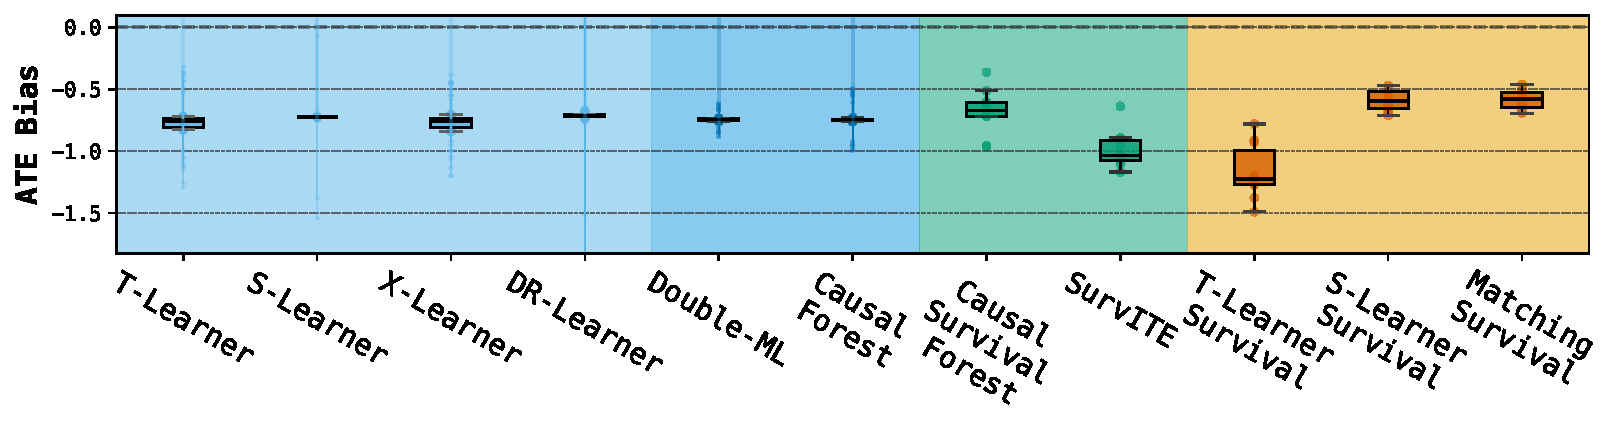
\includegraphics[width=\linewidth]{Appendices/appendix-ch04/images/figure_results_updated/ate_bias/Scenario_D_OBS-NoPos_ate_bias.pdf}
        
    \end{minipage}}
    \hfill
    \subfloat[{RCT: \ChFourBlackCross, Ignorability: \ChFourGrayCheck, Positivity: \ChFourGrayCheck, Ignorable Censoring: \ChFourBlackCross}]{\begin{minipage}[t]{0.49\textwidth}
        \centering
        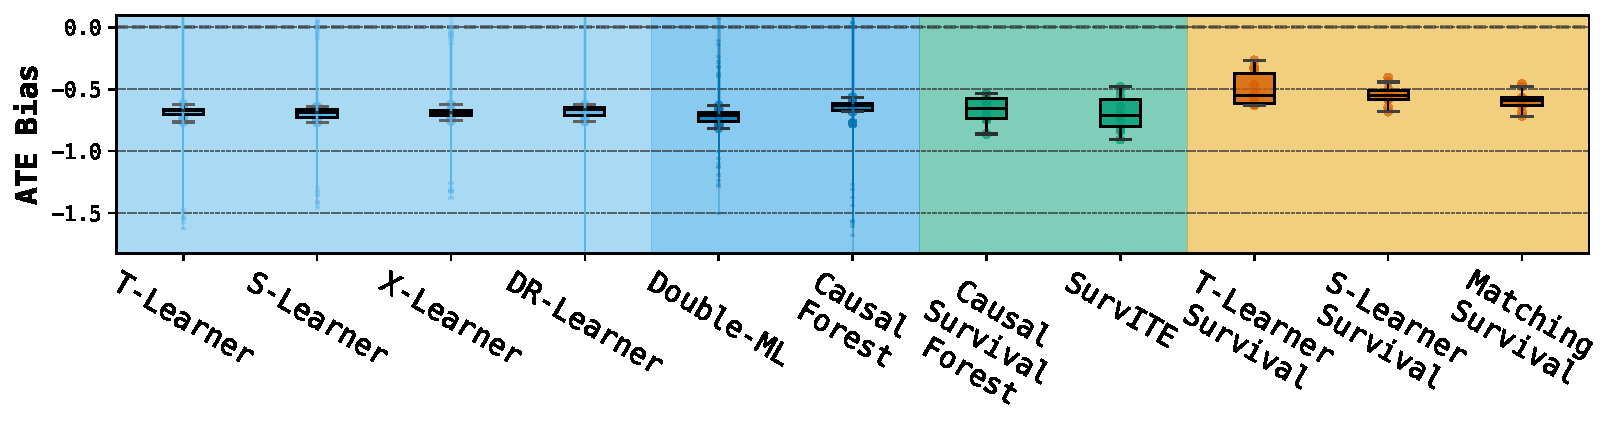
\includegraphics[width=\linewidth]{Appendices/appendix-ch04/images/figure_results_updated/ate_bias/Scenario_D_OBS-CPS-IC_ate_bias.pdf}
        
    \end{minipage}}

    

    \subfloat[{RCT: \ChFourBlackCross, Ignorability: \ChFourBlackCross, Positivity: \ChFourGrayCheck, Ignorable Censoring: \ChFourBlackCross}]{\begin{minipage}[t]{0.49\textwidth}
        \centering
        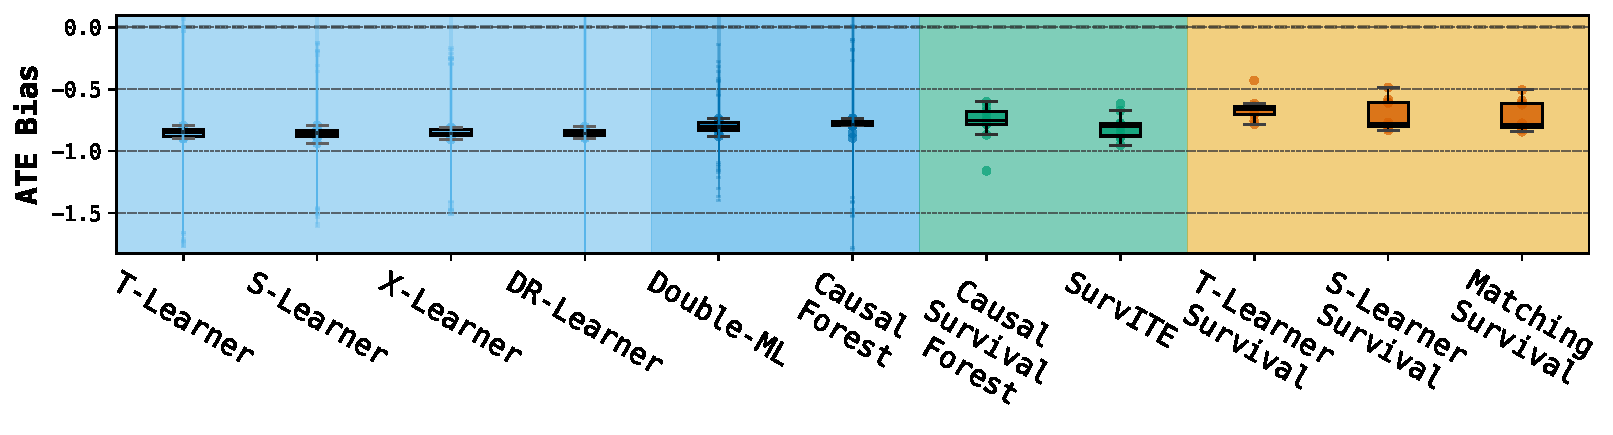
\includegraphics[width=\linewidth]{Appendices/appendix-ch04/images/figure_results_updated/ate_bias/Scenario_D_OBS-UConf-IC_ate_bias.pdf}
        
    \end{minipage}}
    \hfill
    \subfloat[{RCT: \ChFourBlackCross, Ignorability: \ChFourGrayCheck, Positivity: \ChFourBlackCross, Ignorable Censoring: \ChFourBlackCross}]{\begin{minipage}[t]{0.49\textwidth}
        \centering
        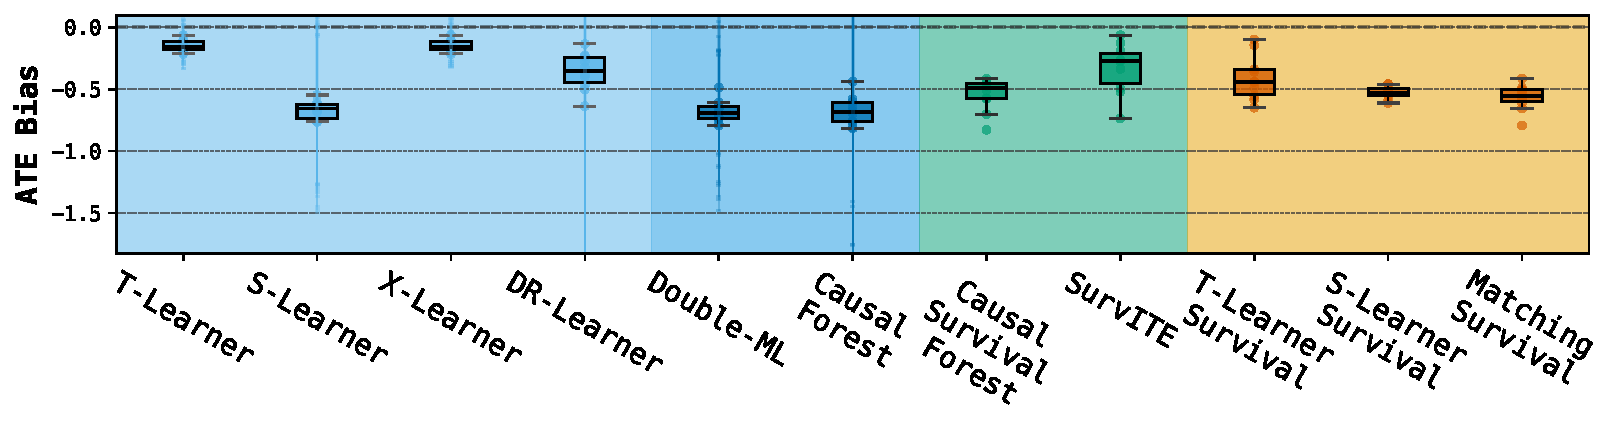
\includegraphics[width=\linewidth]{Appendices/appendix-ch04/images/figure_results_updated/ate_bias/Scenario_D_OBS-NoPos-IC_ate_bias.pdf}
        
    \end{minipage}}

                    \end{minipage}%
    }

    
    
}
\end{figure}



% 

% Secnario E

% !TeX root = ../../../main.tex
\begin{figure}[htbp]
\ChFourFloatContents{ch04:fig:ate_bias_grid_scenario_E}{\caption{ATE Bias across different experiments in Scenario \texttt{E}.}}{
    \centering

            \resizebox{0.95\textwidth}{!}{%
        \begin{minipage}{1\textwidth}

    \subfloat[{RCT: \ChFourGrayCheck (50\%), Ignorability: \ChFourGrayCheck, Positivity: \ChFourGrayCheck, Ign-Censoring: \ChFourGrayCheck}]{\begin{minipage}[t]{0.49\textwidth}
        \centering
        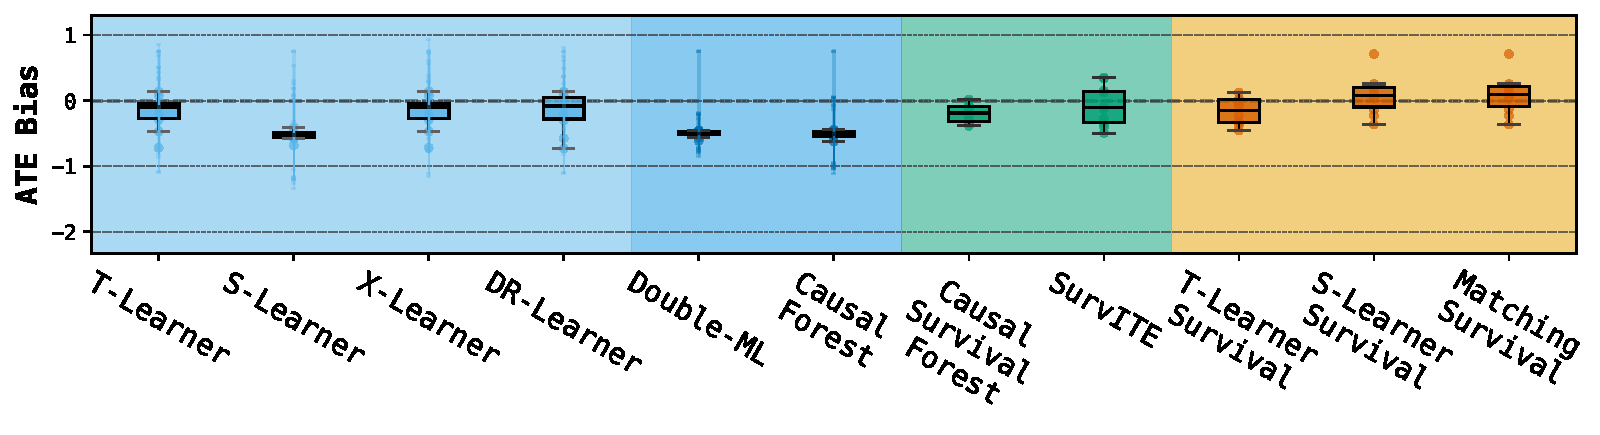
\includegraphics[width=\linewidth]{Appendices/appendix-ch04/images/figure_results_updated/ate_bias/Scenario_E_RCT-50_ate_bias.pdf}
        
    \end{minipage}}
    \hfill
    \subfloat[{RCT: \ChFourGrayCheck (5\%), Ignorability: \ChFourGrayCheck, Positivity: \ChFourGrayCheck, Ign-Censoring: \ChFourGrayCheck}]{\begin{minipage}[t]{0.49\textwidth}
        \centering
        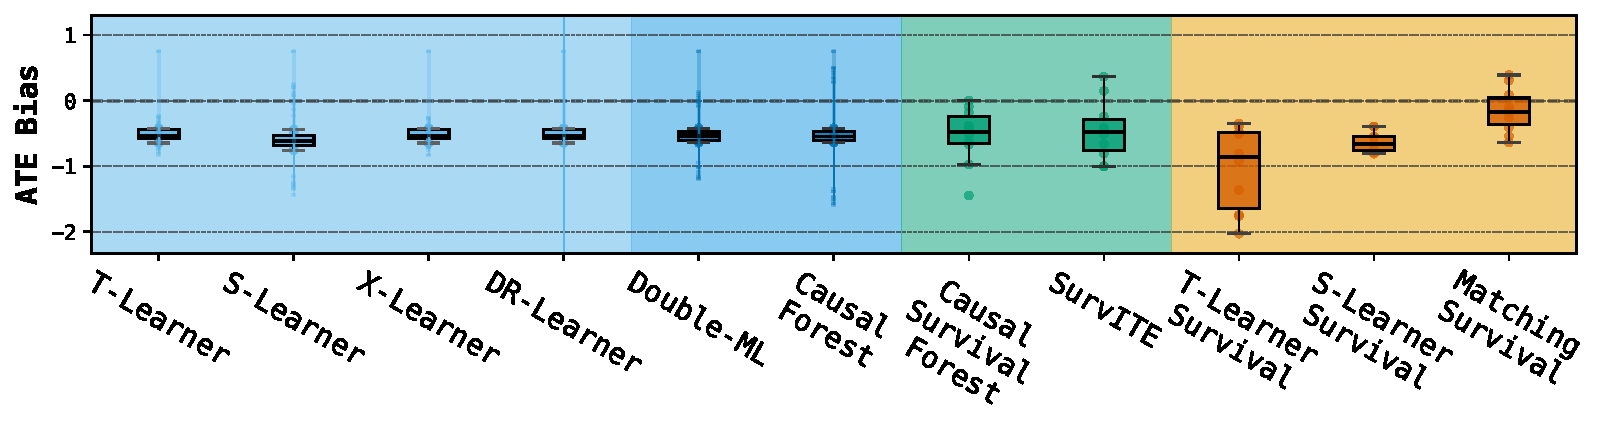
\includegraphics[width=\linewidth]{Appendices/appendix-ch04/images/figure_results_updated/ate_bias/Scenario_E_RCT-5_ate_bias.pdf}
        
    \end{minipage}}

    

    \subfloat[{RCT: \ChFourBlackCross, Ignorability: \ChFourGrayCheck, Positivity: \ChFourGrayCheck, Ignorable Censoring: \ChFourGrayCheck}]{\begin{minipage}[t]{0.49\textwidth}
        \centering
        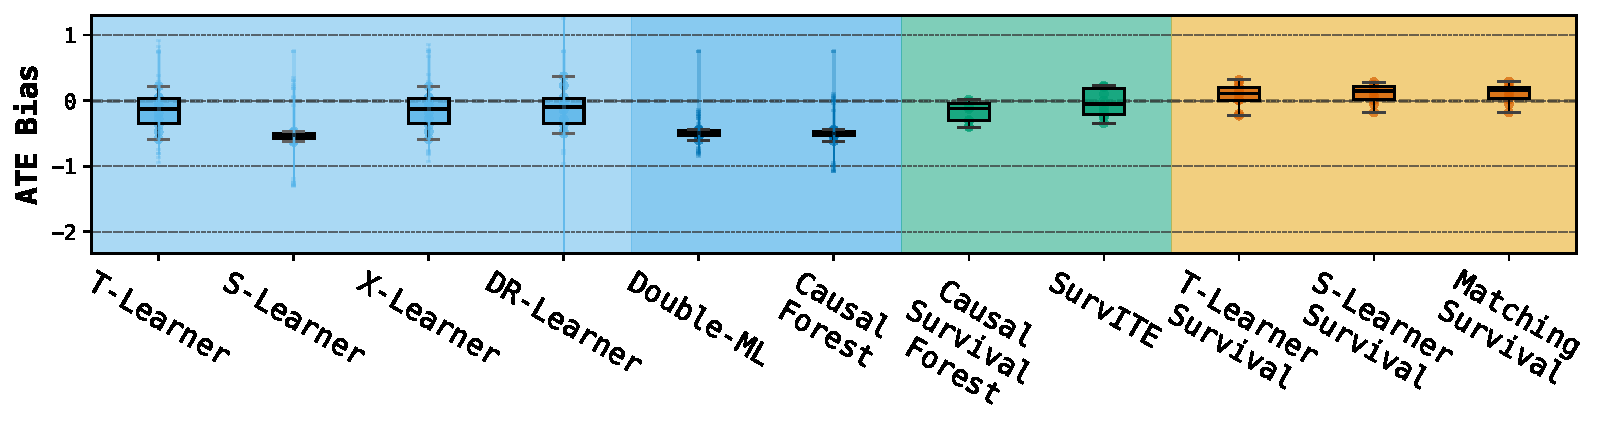
\includegraphics[width=\linewidth]{Appendices/appendix-ch04/images/figure_results_updated/ate_bias/Scenario_E_OBS-CPS_ate_bias.pdf}
        
    \end{minipage}}
    \hfill
    \subfloat[{RCT: \ChFourBlackCross, Ignorability: \ChFourBlackCross, Positivity: \ChFourGrayCheck, Ignorable Censoring: \ChFourGrayCheck}]{\begin{minipage}[t]{0.49\textwidth}
        \centering
        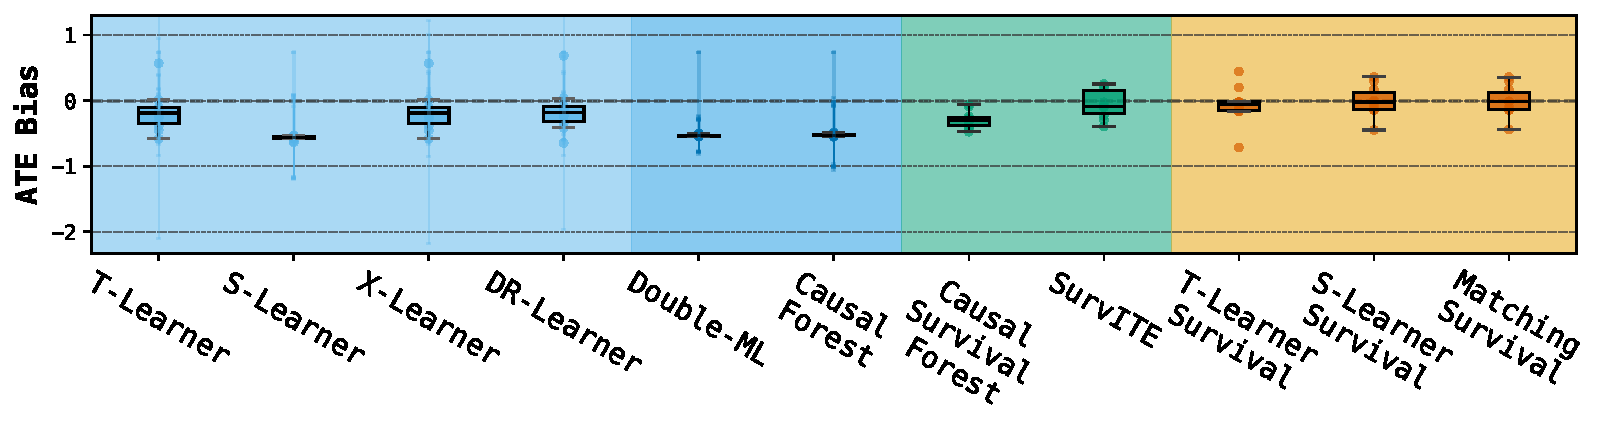
\includegraphics[width=\linewidth]{Appendices/appendix-ch04/images/figure_results_updated/ate_bias/Scenario_E_OBS-UConf_ate_bias.pdf}
        
    \end{minipage}}

    

    \subfloat[{RCT: \ChFourBlackCross, Ignorability: \ChFourGrayCheck, Positivity: \ChFourBlackCross, Ignorable Censoring: \ChFourGrayCheck}]{\begin{minipage}[t]{0.49\textwidth}
        \centering
        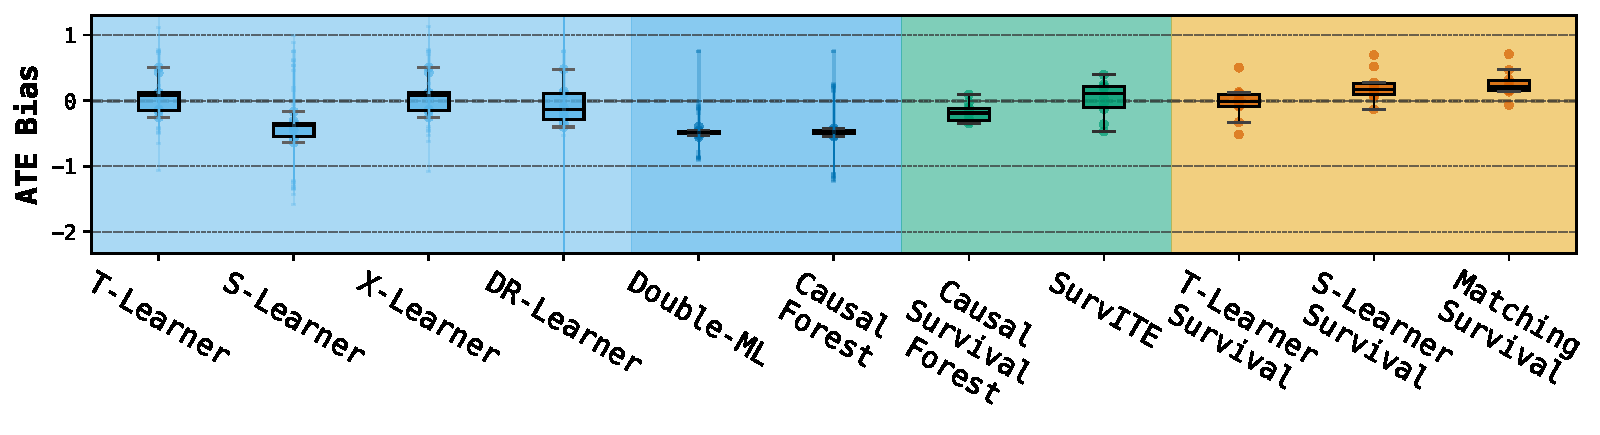
\includegraphics[width=\linewidth]{Appendices/appendix-ch04/images/figure_results_updated/ate_bias/Scenario_E_OBS-NoPos_ate_bias.pdf}
        
    \end{minipage}}
    \hfill
    \subfloat[{RCT: \ChFourBlackCross, Ignorability: \ChFourGrayCheck, Positivity: \ChFourGrayCheck, Ignorable Censoring: \ChFourBlackCross}]{\begin{minipage}[t]{0.49\textwidth}
        \centering
        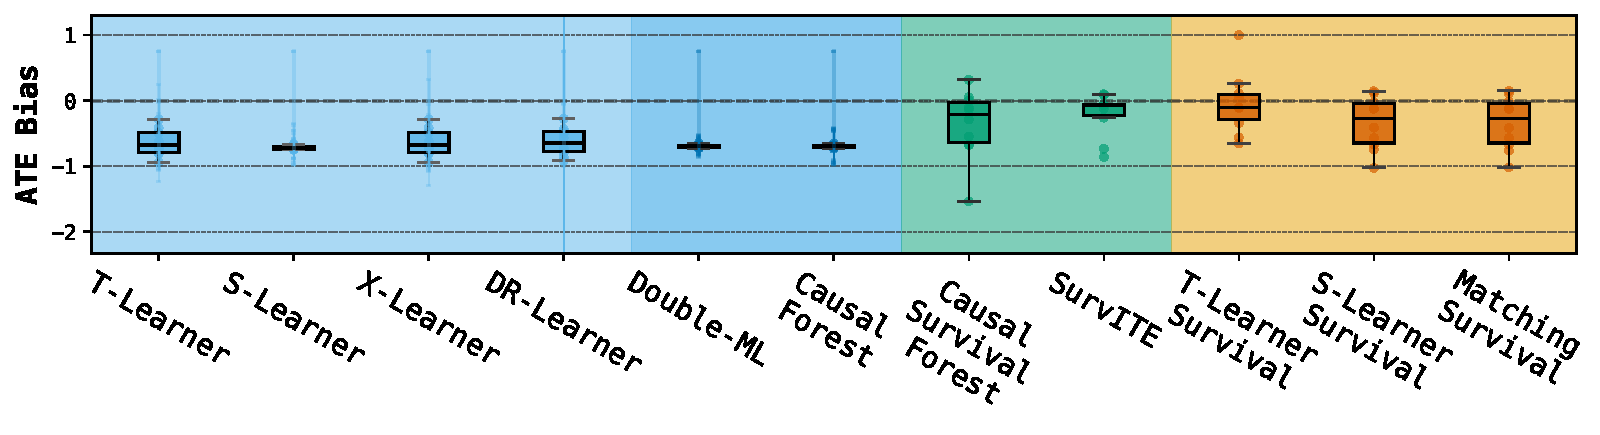
\includegraphics[width=\linewidth]{Appendices/appendix-ch04/images/figure_results_updated/ate_bias/Scenario_E_OBS-CPS-IC_ate_bias.pdf}
        
    \end{minipage}}

    

    \subfloat[{RCT: \ChFourBlackCross, Ignorability: \ChFourBlackCross, Positivity: \ChFourGrayCheck, Ignorable Censoring: \ChFourBlackCross}]{\begin{minipage}[t]{0.49\textwidth}
        \centering
        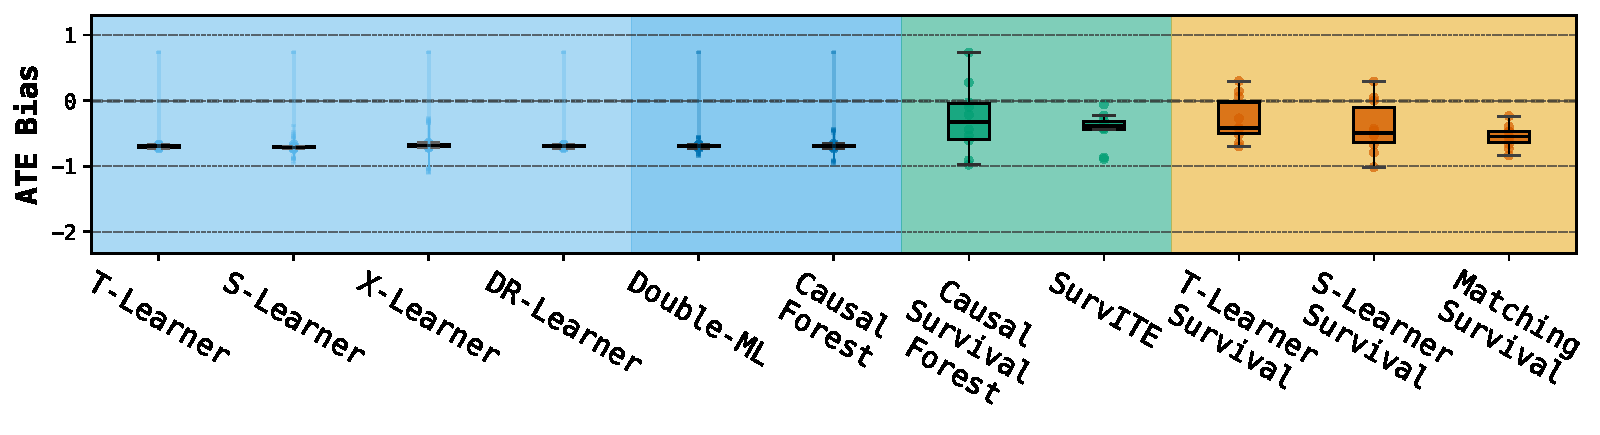
\includegraphics[width=\linewidth]{Appendices/appendix-ch04/images/figure_results_updated/ate_bias/Scenario_E_OBS-UConf-IC_ate_bias.pdf}
        
    \end{minipage}}
    \hfill
    \subfloat[{RCT: \ChFourBlackCross, Ignorability: \ChFourGrayCheck, Positivity: \ChFourBlackCross, Ignorable Censoring: \ChFourBlackCross}]{\begin{minipage}[t]{0.49\textwidth}
        \centering
        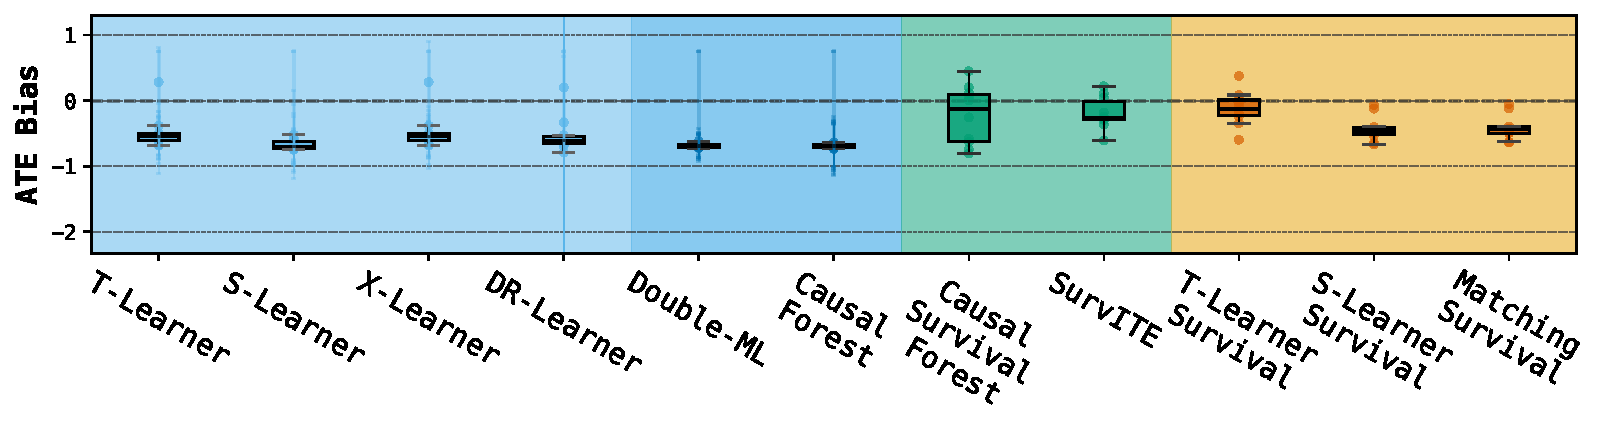
\includegraphics[width=\linewidth]{Appendices/appendix-ch04/images/figure_results_updated/ate_bias/Scenario_E_OBS-NoPos-IC_ate_bias.pdf}
        
    \end{minipage}}

                    \end{minipage}%
    }

    
    
}
\end{figure}






\subsubsection{Evaluation on auxiliary imputation and base learners}\label{ch04:app:auxiliary-eval-results}

In this section, we report the performance of auxiliary imputation and base regression or survival learners on the test sets.

\paragraph{Imputation evaluation}\label{ch04:subapp:impute-eval}

Table~\ref{ch04:tab:impute-eval} reports the MAE of the three imputation methods (Pseudo-obs, Margin, IPCW-T) across eight causal configurations and five censoring scenarios on the test sets.
Recall that Scenarios \texttt{A} and \texttt{B} have low censoring ($<$30\%), Scenario \texttt{C} medium (30--70\%), and Scenarios \texttt{D} and \texttt{E} high ($>$70\%), except it is switched in \texttt{-InfC} causal configurations, as mentioned in Appendix~\ref{ch04:app:synthetic-dataset}.
We can tell that the imputation method Pseudo-obs is only competitive under minimal censoring and suffers from high variability.
Margin imputation provides the best balance of accuracy and robustness, especially as censoring intensifies.
IPCW-T imputation improves over Pseudo-obs in most cases, but generally underperforms relative to Margin in medium‐ and high‐censor contexts.


% !TeX root = ../../../main.tex
\begin{table}[htbp]
\ChFourFloatContents{ch04:tab:impute-eval}{\caption{Evaluation on imputation methods across different survival scenarios and causal configurations. MAE between the imputed and true event times on testing set is reported as mean $\pm$ std. over 10 experimental repeats. ``Total Win'' row counts the number of survival configurations $\times$ random split combinations (8 × 10 = 80) in which each method achieved the lowest MAE, and is calculated within each scenario. The same rule applies to all the tables below in Appendix~\ref{ch04:app:auxiliary-eval-results}.}}{
    \centering
    
    
    \begin{adjustbox}{max width = 0.6\textwidth}
    \begin{tabular}{clccc}
    \toprule
        \multirow{2}{*}{\makecell[l]{\textbf{Survival}\\\textbf{Scenario}}} & \multirow{2}{*}{\makecell[l]{\textbf{Causal}\\\textbf{Configuration}}} & \multicolumn{3}{c}{\textbf{Imputation Method}}                   \\
    \cmidrule(r){3-5}
         &  & \textbf{Pseudo-obs} & \textbf{Margin} & \textbf{IPCW-T} \\ 
    \midrule
        \multirow{9}{*}{\texttt{A}}  & \texttt{RCT-50} & \ChFourBfTab{0.437$\pm$0.021} & 0.446$\pm$0.025 & 0.470$\pm$0.027 \\ 
        ~ & \texttt{RCT-5} & \ChFourBfTab{0.378$\pm$0.027} & 0.387$\pm$0.029 & 0.405$\pm$0.032 \\ 
        ~ & \texttt{OBS-CPS} & \ChFourBfTab{0.448$\pm$0.014} & 0.459$\pm$0.014 & 0.481$\pm$0.015 \\ 
        ~ & \texttt{OBS-UConf} & \ChFourBfTab{0.423$\pm$0.026} & 0.520$\pm$0.028 & 0.455$\pm$0.03 \\ 
        ~ & \texttt{OBS-NoPos} & \ChFourBfTab{0.411$\pm$0.023} & 0.420$\pm$0.023 & 0.442$\pm$0.025 \\ 
        ~ & \texttt{OBS-CPS-InfC} & 0.390$\pm$0.020 & \ChFourBfTab{0.374$\pm$0.014} & 0.388$\pm$0.014 \\ 
        ~ & \texttt{OBS-UConf-InfC} & 0.369$\pm$0.029 & 0.482$\pm$0.027 & \ChFourBfTab{0.362$\pm$0.028} \\ 
        ~ & \texttt{OBS-NoPos-InfC} & 0.347$\pm$0.023 & \ChFourBfTab{0.336$\pm$0.024} & 0.349$\pm$0.026 \\ 
    \cmidrule(r){2-5}
         & Total Win & 51 & 21 & 8 \\ 
    \midrule
        \multirow{9}{*}{\texttt{B}}  & \texttt{RCT-50} & 0.061$\pm$0.005 & 0.05$\pm$0.003 & \ChFourBfTab{0.048$\pm$0.004} \\ 
        ~ & \texttt{RCT-5} & 0.027$\pm$0.003 & 0.022$\pm$0.002 & \ChFourBfTab{0.021$\pm$0.003} \\ 
        ~ & \texttt{OBS-CPS} & 0.052$\pm$0.005 & 0.042$\pm$0.004 & \ChFourBfTab{0.040$\pm$0.003} \\ 
        ~ & \texttt{OBS-UConf} & 0.058$\pm$0.004 & 0.152$\pm$0.007 & \ChFourBfTab{0.046$\pm$0.004} \\ 
        ~ & \texttt{OBS-NoPos} & 0.068$\pm$0.008 & 0.057$\pm$0.005 & \ChFourBfTab{0.056$\pm$0.005} \\ 
        ~ & \texttt{OBS-CPS-InfC} & 0.039$\pm$0.005 & 0.037$\pm$0.005 & \ChFourBfTab{0.036$\pm$0.005} \\ 
        ~ & \texttt{OBS-UConf-InfC} & 0.040$\pm$0.004 & 0.140$\pm$0.005 & \ChFourBfTab{0.038$\pm$0.004} \\ 
        ~ & \texttt{OBS-NoPos-InfC} & 0.048$\pm$0.007 & 0.046$\pm$0.008 & \ChFourBfTab{0.045$\pm$0.008} \\ 
    \cmidrule(r){2-5}
         & Total Win & 0 & 3 & 77 \\ 
    \midrule
        \multirow{9}{*}{\texttt{C}}  & \texttt{RCT-50} & \ChFourBfTab{0.837$\pm$0.008} & 0.838$\pm$0.008 & 0.841$\pm$0.007 \\ 
        ~ & \texttt{RCT-5} & 0.803$\pm$0.013 & 0.804$\pm$0.013 & \ChFourBfTab{0.793$\pm$0.009} \\ 
        ~ & \texttt{OBS-CPS} & 0.829$\pm$0.014 & 0.830$\pm$0.014 & \ChFourBfTab{0.828$\pm$0.014} \\ 
        ~ & \texttt{OBS-UConf} & \ChFourBfTab{0.835$\pm$0.026} & 2.701$\pm$0.033 & 0.837$\pm$0.027 \\ 
        ~ & \texttt{OBS-NoPos} & \ChFourBfTab{0.845$\pm$0.014} & \ChFourBfTab{0.845$\pm$0.015} & 0.855$\pm$0.012 \\ 
        ~ & \texttt{OBS-CPS-InfC} & 2.786$\pm$0.079 & \ChFourBfTab{2.090$\pm$0.046} & 2.858$\pm$0.055 \\ 
        ~ & \texttt{OBS-UConf-InfC} & \ChFourBfTab{2.753$\pm$0.074} & 2.443$\pm$0.023 & 2.852$\pm$0.058 \\ 
        ~ & \texttt{OBS-NoPos-InfC} & 2.904$\pm$0.061 & \ChFourBfTab{2.197$\pm$0.045} & 3.006$\pm$0.034 \\ 
    \cmidrule(r){2-5}
         & Total Win & 23 & 35 & 22 \\ 
    \midrule
        \multirow{9}{*}{\texttt{D}}  & \texttt{RCT-50} & 3.303$\pm$0.333 & \ChFourBfTab{2.241$\pm$0.065} & 2.624$\pm$0.054 \\ 
        ~ & \texttt{RCT-5} & 2.897$\pm$0.257 & \ChFourBfTab{1.845$\pm$0.059} & 2.192$\pm$0.059 \\ 
        ~ & \texttt{OBS-CPS} & 3.191$\pm$0.449 & \ChFourBfTab{2.109$\pm$0.062} & 2.421$\pm$0.068 \\ 
        ~ & \texttt{OBS-UConf} & 3.463$\pm$0.706 & \ChFourBfTab{2.361$\pm$0.198} & 2.610$\pm$0.073 \\ 
        ~ & \texttt{OBS-NoPos} & 3.536$\pm$0.435 & \ChFourBfTab{2.404$\pm$0.074} & 2.853$\pm$0.072 \\ 
        ~ & \texttt{OBS-CPS-InfC} & 1.395$\pm$0.067 & \ChFourBfTab{1.289$\pm$0.064} & 1.366$\pm$0.068 \\ 
        ~ & \texttt{OBS-UConf-InfC} & 1.524$\pm$0.069 & 1.737$\pm$0.054 & \ChFourBfTab{1.511$\pm$0.063} \\ 
        ~ & \texttt{OBS-NoPos-InfC} & 1.689$\pm$0.074 & \ChFourBfTab{1.595$\pm$0.069} & 1.698$\pm$0.073 \\ 
    \cmidrule(r){2-5}
        & Total Win & 3 & 68 & 9 \\ 
    \midrule
        \multirow{9}{*}{\texttt{E}}  & \texttt{RCT-50} & 2.672$\pm$0.348 & \ChFourBfTab{1.595$\pm$0.019} & 2.033$\pm$0.022 \\ 
        ~ & \texttt{RCT-5} & 2.238$\pm$0.218 & \ChFourBfTab{1.468$\pm$0.023} & 1.823$\pm$0.023 \\ 
        ~ & \texttt{OBS-CPS} & 2.446$\pm$0.262 & \ChFourBfTab{1.577$\pm$0.022} & 1.992$\pm$0.032 \\ 
        ~ & \texttt{OBS-UConf} & 2.531$\pm$0.191 & 2.651$\pm$0.054 & \ChFourBfTab{2.051$\pm$0.031} \\ 
        ~ & \texttt{OBS-NoPos} & 2.669$\pm$0.288 & \ChFourBfTab{1.639$\pm$0.021} & 2.102$\pm$0.035 \\ 
        ~ & \texttt{OBS-CPS-InfC} & 3.324$\pm$0.136 & \ChFourBfTab{2.483$\pm$0.05} & 3.491$\pm$0.054 \\ 
        ~ & \texttt{OBS-UConf-InfC} & 3.346$\pm$0.147 & \ChFourBfTab{2.686$\pm$0.071} & 3.526$\pm$0.036 \\ 
        ~ & \texttt{OBS-NoPos-InfC} & 3.373$\pm$0.101 & \ChFourBfTab{2.541$\pm$0.038} & 3.648$\pm$0.072 \\  
    \cmidrule(r){2-5}
         & Total Win & 0 & 70 & 10 \\ 
    \bottomrule
    \end{tabular}
    \end{adjustbox}
}
\end{table}



\paragraph{Base regression learner evaluation} \label{ch04:subapp:base-reg-eval}
See Table~\ref{ch04:tab:base-s-learner}, \ref{ch04:tab:base-t-learner}, \ref{ch04:tab:base-x-learner}, \ref{ch04:tab:base-dr-learner} for MAE of prediction by the base regression learners for S-, T-, X-, DR-Learners.
The MAE is calculated by comparing a base learner's predicted event times and imputed event times by the imputation method (the latter is used as the ``ground truth'' for the base regression learners).
Since there are three imputation methods used, we first take the average of MAE across three different imputation methods within each random split, then report the mean and standard deviation of the average MAE across 10 experimental repeats with different random splits. 

See Table~\ref{ch04:tab:base-dr-learner-propensity} for the AUC on the evaluation of the predicted propensity score of DR-Learners.


% !TeX root = ../../../main.tex
\begin{table}[htbp]
\ChFourFloatContents{ch04:tab:base-s-learner}{\caption{S-Learner MAE}}{
    \centering
     
    \begin{adjustbox}{max width = 0.6\textwidth}
    \begin{tabular}{clccc}
    \toprule
        \multirow{2}{*}{\makecell[l]{\textbf{Survival}\\\textbf{Scenario}}} & \multirow{2}{*}{\makecell[l]{\textbf{Causal}\\\textbf{Configuration}}} & \multicolumn{3}{c}{\textbf{Base Regression Model}} \\ 
        \cmidrule(r){3-5}
         & & \textbf{Lasso Reg.} & \textbf{Random Forest} & \textbf{XGBoost} \\
    \midrule
        \multirow{9}{*}{\texttt{A}}   & \texttt{RCT-50} & 0.661$\pm$0.012 & \ChFourBfTab{0.655$\pm$0.014} & 0.671$\pm$0.013 \\ 
        ~ & \texttt{RCT-5} & \ChFourBfTab{0.645$\pm$0.011} & 0.649$\pm$0.012 & 0.667$\pm$0.014 \\ 
        ~ & \texttt{OBS-CPS} & 0.653$\pm$0.011 & \ChFourBfTab{0.646$\pm$0.010} & 0.662$\pm$0.012 \\ 
        ~ & \texttt{OBS-UConf} & \ChFourBfTab{0.604$\pm$0.009} & 0.608$\pm$0.009 & 0.620$\pm$0.007 \\ 
        ~ & \texttt{OBS-NoPos} & 0.657$\pm$0.010 & \ChFourBfTab{0.654$\pm$0.011} & 0.671$\pm$0.013 \\ 
        ~ & \texttt{OBS-CPS-InfC} & \ChFourBfTab{0.727$\pm$0.018} & 0.730$\pm$0.021 & 0.752$\pm$0.023 \\ 
        ~ & \texttt{OBS-UConf-InfC} & \ChFourBfTab{0.675$\pm$0.019} & 0.693$\pm$0.023 & 0.713$\pm$0.023 \\ 
        ~ & \texttt{OBS-NoPos-InfC} & \ChFourBfTab{0.724$\pm$0.014} & 0.732$\pm$0.018 & 0.755$\pm$0.02 \\ 
        \cmidrule(r){2-5}
        ~ & Total Win & 44 & 36 & 0 \\ 
    \midrule
        \multirow{9}{*}{\texttt{B}} & \texttt{RCT-50} & 0.33$\pm$0.008 & \ChFourBfTab{0.315$\pm$0.011} & 0.334$\pm$0.015 \\ 
        ~ & \texttt{RCT-5} & 0.278$\pm$0.006 & \ChFourBfTab{0.277$\pm$0.006} & 0.292$\pm$0.008 \\ 
        ~ & \texttt{OBS-CPS} & 0.315$\pm$0.011 & \ChFourBfTab{0.307$\pm$0.012} & 0.324$\pm$0.019 \\ 
        ~ & \texttt{OBS-UConf} & 0.354$\pm$0.007 & \ChFourBfTab{0.341$\pm$0.008} & 0.359$\pm$0.011 \\ 
        ~ & \texttt{OBS-NoPos} & 0.345$\pm$0.009 & \ChFourBfTab{0.323$\pm$0.011} & 0.341$\pm$0.011 \\ 
        ~ & \texttt{OBS-CPS-InfC} & 0.301$\pm$0.007 & \ChFourBfTab{0.294$\pm$0.006} & 0.309$\pm$0.008 \\ 
        ~ & \texttt{OBS-UConf-InfC} & 0.34$\pm$0.004 & \ChFourBfTab{0.328$\pm$0.005} & 0.347$\pm$0.006 \\ 
        ~ & \texttt{OBS-NoPos-InfC} & 0.337$\pm$0.005 & \ChFourBfTab{0.319$\pm$0.006} & 0.337$\pm$0.007 \\ 
        \cmidrule(r){2-5}
        ~ & Total Win & 3 & 77 & 0 \\ 
    \midrule
        \multirow{9}{*}{\texttt{C}} & \texttt{RCT-50} & \ChFourBfTab{1.430$\pm$0.022} & 1.593$\pm$0.025 & 1.738$\pm$0.024 \\ 
        ~ & \texttt{RCT-5} & \ChFourBfTab{1.403$\pm$0.019} & 1.532$\pm$0.018 & 1.687$\pm$0.027 \\ 
        ~ & \texttt{OBS-CPS} & \ChFourBfTab{1.409$\pm$0.021} & 1.555$\pm$0.025 & 1.706$\pm$0.028 \\ 
        ~ & \texttt{OBS-UConf} & \ChFourBfTab{1.419$\pm$0.023} & 1.563$\pm$0.026 & 1.721$\pm$0.020 \\ 
        ~ & \texttt{OBS-NoPos} & \ChFourBfTab{1.453$\pm$0.019} & 1.612$\pm$0.024 & 1.755$\pm$0.022 \\ 
        ~ & \texttt{OBS-CPS-InfC} & \ChFourBfTab{0.931$\pm$0.027} & 1.011$\pm$0.03 & 1.148$\pm$0.045 \\ 
        ~ & \texttt{OBS-UConf-InfC} & \ChFourBfTab{0.895$\pm$0.033} & 0.966$\pm$0.04 & 1.096$\pm$0.059 \\ 
        ~ & \texttt{OBS-NoPos-InfC} & \ChFourBfTab{0.916$\pm$0.057} & 1.003$\pm$0.067 & 1.123$\pm$0.086 \\ 
        \cmidrule(r){2-5}
        ~ & Total Win & 80 & 0 & 0 \\ 
    \midrule
        \multirow{9}{*}{\texttt{D}} & \texttt{RCT-50} & \ChFourBfTab{0.941$\pm$0.18} & 1.002$\pm$0.202 & 1.082$\pm$0.206 \\ 
        ~ & \texttt{RCT-5} & \ChFourBfTab{1.016$\pm$0.121} & 1.095$\pm$0.123 & 1.210$\pm$0.248 \\ 
        ~ & \texttt{OBS-CPS} & \ChFourBfTab{1.031$\pm$0.258} & 1.082$\pm$0.264 & 1.188$\pm$0.345 \\ 
        ~ & \texttt{OBS-UConf} & \ChFourBfTab{0.985$\pm$0.34} & 1.015$\pm$0.300 & 1.073$\pm$0.383 \\ 
        ~ & \texttt{OBS-NoPos} & \ChFourBfTab{0.967$\pm$0.238} & 1.03$\pm$0.249 & 1.107$\pm$0.295 \\ 
        ~ & \texttt{OBS-CPS-InfC} & \ChFourBfTab{1.146$\pm$0.030} & 1.148$\pm$0.034 & 1.209$\pm$0.044 \\ 
        ~ & \texttt{OBS-UConf-InfC} & 1.179$\pm$0.024 & \ChFourBfTab{1.172$\pm$0.031} & 1.234$\pm$0.032 \\ 
        ~ & \texttt{OBS-NoPos-InfC} & \ChFourBfTab{1.169$\pm$0.026} & \ChFourBfTab{1.169$\pm$0.026} & 1.230$\pm$0.028 \\ 
        \cmidrule(r){2-5}
        ~ & Total Win & 48 & 29 & 3 \\ 
    \midrule
        \multirow{9}{*}{\texttt{E}} & \texttt{RCT-50} & \ChFourBfTab{1.75$\pm$0.186} & 1.906$\pm$0.207 & 2.124$\pm$0.247 \\ 
        ~ & \texttt{RCT-5} & \ChFourBfTab{1.604$\pm$0.125} & 1.731$\pm$0.133 & 1.901$\pm$0.17 \\ 
        ~ & \texttt{OBS-CPS} & \ChFourBfTab{1.651$\pm$0.161} & 1.799$\pm$0.201 & 1.990$\pm$0.243 \\ 
        ~ & \texttt{OBS-UConf} & \ChFourBfTab{1.630$\pm$0.127} & 1.779$\pm$0.159 & 1.974$\pm$0.212 \\ 
        ~ & \texttt{OBS-NoPos} & \ChFourBfTab{1.698$\pm$0.139} & 1.856$\pm$0.162 & 2.059$\pm$0.202 \\ 
        ~ & \texttt{OBS-CPS-InfC} & \ChFourBfTab{0.917$\pm$0.089} & 1.012$\pm$0.113 & 1.140$\pm$0.141 \\ 
        ~ & \texttt{OBS-UConf-InfC} & \ChFourBfTab{0.968$\pm$0.130} & 1.074$\pm$0.164 & 1.222$\pm$0.237 \\ 
        ~ & \texttt{OBS-NoPos-InfC} & \ChFourBfTab{0.928$\pm$0.060} & 1.012$\pm$0.063 & 1.130$\pm$0.071 \\ 
        \cmidrule(r){2-5}
        ~ & Total Win & 80 & 0 & 0 \\ 
    \bottomrule
    \end{tabular}
    \end{adjustbox}
}
\end{table}




% !TeX root = ../../../main.tex
\begin{table}[htbp]
\ChFourFloatContents{ch04:tab:base-t-learner}{\caption{T-Learner MAE}}{
    \centering
     
    \begin{adjustbox}{max width=1\textwidth}
    \begin{tabular}{clccc|ccc}
    \toprule
        \multirow{2}{*}{\makecell[l]{\textbf{Survival}\\\textbf{Scenario}}} & \multirow{2}{*}{\makecell[l]{\textbf{Causal}\\\textbf{Configuration}}} & \multicolumn{3}{c}{\textbf{Base Regression Model (Treated)}} & \multicolumn{3}{c}{\textbf{Base Regression Model (Control)}} \\ 
        \cmidrule(r){3-5} \cmidrule(r){6-8}
        & & \textbf{Lasso Reg.} & \textbf{Random Forest} & \textbf{XGBoost} & \textbf{Lasso Reg.} & \textbf{Random Forest} & \textbf{XGBoost} \\
        \midrule
        \multirow{9}{*}{\texttt{A}} & \texttt{RCT-50} & 0.669$\pm$0.012 & \ChFourBfTab{0.652$\pm$0.013} & 0.680$\pm$0.015 & \ChFourBfTab{0.652$\pm$0.019} & 0.657$\pm$0.019 & 0.685$\pm$0.019 \\ 
        ~ &\texttt{RCT-5} & 0.656$\pm$0.044 & \ChFourBfTab{0.641$\pm$0.049} & 0.677$\pm$0.050 & \ChFourBfTab{0.644$\pm$0.011} & 0.650$\pm$0.012 & 0.668$\pm$0.014 \\ 
        ~ &\texttt{OBS-CPS} & 0.711$\pm$0.012 & \ChFourBfTab{0.697$\pm$0.012} & 0.727$\pm$0.012 & \ChFourBfTab{0.588$\pm$0.014} & 0.595$\pm$0.014 & 0.621$\pm$0.018 \\ 
        ~ &\texttt{OBS-UConf} & \ChFourBfTab{0.640$\pm$0.009} & 0.641$\pm$0.007 & 0.668$\pm$0.005 & \ChFourBfTab{0.558$\pm$0.012} & 0.566$\pm$0.013 & 0.593$\pm$0.015 \\ 
        ~ &\texttt{OBS-NoPos} & 0.568$\pm$0.014 & \ChFourBfTab{0.561$\pm$0.013} & 0.587$\pm$0.016 & \ChFourBfTab{0.733$\pm$0.015} & 0.747$\pm$0.016 & 0.776$\pm$0.016 \\ 
        ~ &\texttt{OBS-CPS-InfC} & 0.799$\pm$0.020 & \ChFourBfTab{0.797$\pm$0.022} & 0.838$\pm$0.023 & \ChFourBfTab{0.646$\pm$0.023} & 0.664$\pm$0.025 & 0.699$\pm$0.029 \\ 
        ~ &\texttt{OBS-UConf-InfC} & \ChFourBfTab{0.723$\pm$0.023} & 0.740$\pm$0.031 & 0.778$\pm$0.030 & \ChFourBfTab{0.614$\pm$0.019} & 0.633$\pm$0.023 & 0.668$\pm$0.025 \\ 
        ~ &\texttt{OBS-NoPos-InfC} & \ChFourBfTab{0.608$\pm$0.018} & 0.609$\pm$0.016 & 0.642$\pm$0.020 & \ChFourBfTab{0.824$\pm$0.021} & 0.855$\pm$0.021 & 0.895$\pm$0.029 \\ 
        \cmidrule(r){2-5} \cmidrule(r){6-8}
        ~ &Total Win & 28 & 52 & 0 & 77 & 3 & 0 \\ 
        \midrule
        \multirow{9}{*}{\texttt{B}} & \texttt{RCT-50} & 0.375$\pm$0.012 & \ChFourBfTab{0.350$\pm$0.014} & 0.374$\pm$0.016 & \ChFourBfTab{0.279$\pm$0.007} & 0.281$\pm$0.008 & 0.303$\pm$0.006 \\ 
        ~ & \texttt{RCT-5} & 0.393$\pm$0.051 & \ChFourBfTab{0.383$\pm$0.047} & 0.404$\pm$0.043 & \ChFourBfTab{0.271$\pm$0.005} & 0.273$\pm$0.005 & 0.287$\pm$0.006 \\ 
        ~ & \texttt{OBS-CPS} & 0.326$\pm$0.014 & \ChFourBfTab{0.302$\pm$0.014} & 0.322$\pm$0.016 & \ChFourBfTab{0.305$\pm$0.011} & 0.313$\pm$0.012 & 0.338$\pm$0.015 \\ 
        ~ & \texttt{OBS-UConf} & 0.375$\pm$0.008 & \ChFourBfTab{0.348$\pm$0.009} & 0.371$\pm$0.011 & \ChFourBfTab{0.327$\pm$0.008} & 0.334$\pm$0.007 & 0.363$\pm$0.012 \\ 
        ~ & \texttt{OBS-NoPos} & 0.425$\pm$0.014 & \ChFourBfTab{0.411$\pm$0.015} & 0.442$\pm$0.017 & \ChFourBfTab{0.231$\pm$0.007} & 0.235$\pm$0.007 & 0.253$\pm$0.008 \\ 
        ~ & \texttt{OBS-CPS-InfC} & 0.311$\pm$0.007 & \ChFourBfTab{0.292$\pm$0.006} & 0.311$\pm$0.008 & \ChFourBfTab{0.291$\pm$0.009} & 0.297$\pm$0.010 & 0.322$\pm$0.011 \\ 
        ~ & \texttt{OBS-UConf-InfC} & 0.365$\pm$0.004 & \ChFourBfTab{0.344$\pm$0.007} & 0.370$\pm$0.009 & \ChFourBfTab{0.310$\pm$0.007} & 0.313$\pm$0.007 & 0.337$\pm$0.008 \\ 
        ~ & \texttt{OBS-NoPos-InfC} & 0.415$\pm$0.009 & \ChFourBfTab{0.406$\pm$0.009} & 0.438$\pm$0.011 & \ChFourBfTab{0.228$\pm$0.005} & 0.233$\pm$0.006 & 0.249$\pm$0.006 \\ 
        \cmidrule(r){2-5} \cmidrule(r){6-8}
        ~ & Total Win & 4 & 76 & 0 & 68 & 12 & 0 \\ 
        \midrule
        \multirow{9}{*}{\texttt{C}} & \texttt{RCT-50} & \ChFourBfTab{1.534$\pm$0.037} & 1.653$\pm$0.041 & 1.839$\pm$0.046 & \ChFourBfTab{1.387$\pm$0.029} & 1.542$\pm$0.020 & 1.747$\pm$0.027 \\ 
        ~ & \texttt{RCT-5} & \ChFourBfTab{1.643$\pm$0.091} & 1.751$\pm$0.085 & 1.935$\pm$0.074 & \ChFourBfTab{1.393$\pm$0.020} & 1.527$\pm$0.02 & 1.688$\pm$0.021 \\ 
        ~ & \texttt{OBS-CPS} & \ChFourBfTab{1.484$\pm$0.026} & 1.599$\pm$0.031 & 1.797$\pm$0.036 & \ChFourBfTab{1.379$\pm$0.030} & 1.529$\pm$0.029 & 1.726$\pm$0.033 \\ 
        ~ & \texttt{OBS-UConf} & \ChFourBfTab{1.493$\pm$0.037} & 1.617$\pm$0.034 & 1.809$\pm$0.028 & \ChFourBfTab{1.363$\pm$0.019} & 1.528$\pm$0.021 & 1.740$\pm$0.027 \\ 
        ~ & \texttt{OBS-NoPos} & \ChFourBfTab{1.568$\pm$0.040} & 1.665$\pm$0.038 & 1.860$\pm$0.037 & \ChFourBfTab{1.420$\pm$0.037} & 1.565$\pm$0.027 & 1.763$\pm$0.035 \\ 
        ~ & \texttt{OBS-CPS-InfC} & \ChFourBfTab{0.909$\pm$0.047} & 1.002$\pm$0.052 & 1.144$\pm$0.050 & \ChFourBfTab{0.953$\pm$0.042} & 1.040$\pm$0.048 & 1.198$\pm$0.060 \\ 
        ~ & \texttt{OBS-UConf-InfC} & \ChFourBfTab{0.876$\pm$0.039} & 0.951$\pm$0.052 & 1.088$\pm$0.070 & \ChFourBfTab{0.916$\pm$0.044} & 1.004$\pm$0.056 & 1.166$\pm$0.079 \\ 
        ~ & \texttt{OBS-NoPos-InfC} & \ChFourBfTab{0.902$\pm$0.057} & 1.009$\pm$0.074 & 1.149$\pm$0.088 & \ChFourBfTab{0.928$\pm$0.076} & 1.016$\pm$0.087 & 1.152$\pm$0.088 \\ 
        \cmidrule(r){2-5} \cmidrule(r){6-8}
        ~ & Total Win & 79 & 1 & 0 & 80 & 0 & 0 \\ 
        \midrule
        \multirow{9}{*}{\texttt{D}} & \texttt{RCT-50} & \ChFourBfTab{0.302$\pm$0.083} & 0.316$\pm$0.093 & 0.339$\pm$0.11 & \ChFourBfTab{1.546$\pm$0.304} & 1.691$\pm$0.484 & 1.767$\pm$0.429 \\ 
        ~ & \texttt{RCT-5} & \ChFourBfTab{0.284$\pm$0.044} & 0.296$\pm$0.049 & 0.312$\pm$0.052 & \ChFourBfTab{1.051$\pm$0.127} & 1.118$\pm$0.129 & 1.285$\pm$0.304 \\ 
        ~ & \texttt{OBS-CPS} & \ChFourBfTab{0.347$\pm$0.084} & 0.366$\pm$0.087 & 0.384$\pm$0.094 & \ChFourBfTab{1.651$\pm$0.416} & 1.758$\pm$0.443 & 1.924$\pm$0.594 \\ 
        ~ & \texttt{OBS-UConf} & \ChFourBfTab{0.328$\pm$0.134} & 0.343$\pm$0.130 & 0.362$\pm$0.138 & \ChFourBfTab{1.691$\pm$0.564} & 1.797$\pm$0.529 & 1.809$\pm$0.705 \\ 
        ~ & \texttt{OBS-NoPos} & \ChFourBfTab{0.334$\pm$0.105} & 0.342$\pm$0.117 & 0.366$\pm$0.129 & \ChFourBfTab{1.571$\pm$0.382} & 1.659$\pm$0.392 & 1.939$\pm$0.612 \\ 
        ~ & \texttt{OBS-CPS-InfC} & 1.138$\pm$0.029 & \ChFourBfTab{1.097$\pm$0.027} & 1.171$\pm$0.028 & \ChFourBfTab{1.147$\pm$0.041} & 1.201$\pm$0.051 & 1.300$\pm$0.056 \\ 
        ~ & \texttt{OBS-UConf-InfC} & 1.206$\pm$0.029 & \ChFourBfTab{1.156$\pm$0.043} & 1.240$\pm$0.044 & \ChFourBfTab{1.146$\pm$0.023} & 1.197$\pm$0.028 & 1.298$\pm$0.029 \\ 
        ~ & \texttt{OBS-NoPos-InfC} & 1.216$\pm$0.030 & \ChFourBfTab{1.198$\pm$0.035} & 1.297$\pm$0.046 & \ChFourBfTab{1.100$\pm$0.030} & 1.143$\pm$0.037 & 1.222$\pm$0.035 \\ 
        \cmidrule(r){2-5} \cmidrule(r){6-8}
        ~ & Total Win & 45 & 35 & 0 & 66 & 10 & 4 \\ 
        \midrule
        \multirow{9}{*}{\texttt{E}}  & \texttt{RCT-50} & \ChFourBfTab{1.784$\pm$0.230} & 1.955$\pm$0.255 & 2.22$\pm$0.310 & \ChFourBfTab{1.720$\pm$0.154} & 1.899$\pm$0.184 & 2.108$\pm$0.198 \\ 
        ~ & \texttt{RCT-5} & \ChFourBfTab{1.607$\pm$0.244} & 1.859$\pm$0.436 & 1.969$\pm$0.335 & \ChFourBfTab{1.605$\pm$0.121} & 1.733$\pm$0.131 & 1.894$\pm$0.147 \\ 
        ~ & \texttt{OBS-CPS} & \ChFourBfTab{1.670$\pm$0.194} & 1.852$\pm$0.261 & 2.092$\pm$0.312 & \ChFourBfTab{1.637$\pm$0.141} & 1.785$\pm$0.158 & 1.993$\pm$0.200 \\ 
        ~ & \texttt{OBS-UConf} & \ChFourBfTab{1.650$\pm$0.145} & 1.809$\pm$0.167 & 2.053$\pm$0.239 & \ChFourBfTab{1.616$\pm$0.130} & 1.763$\pm$0.144 & 1.982$\pm$0.201 \\ 
        ~ & \texttt{OBS-NoPos} & \ChFourBfTab{1.740$\pm$0.161} & 1.907$\pm$0.200 & 2.198$\pm$0.338 & \ChFourBfTab{1.663$\pm$0.140} & 1.804$\pm$0.148 & 2.027$\pm$0.167 \\ 
        ~ & \texttt{OBS-CPS-InfC} & \ChFourBfTab{0.911$\pm$0.111} & 1.007$\pm$0.123 & 1.146$\pm$0.140 & \ChFourBfTab{0.925$\pm$0.074} & 1.015$\pm$0.096 & 1.158$\pm$0.104 \\ 
        ~ & \texttt{OBS-UConf-InfC} & \ChFourBfTab{0.953$\pm$0.107} & 1.049$\pm$0.118 & 1.221$\pm$0.146 & \ChFourBfTab{0.987$\pm$0.159} & 1.103$\pm$0.222 & 1.271$\pm$0.228 \\ 
        ~ & \texttt{OBS-NoPos-InfC} & \ChFourBfTab{0.949$\pm$0.085} & 1.043$\pm$0.095 & 1.221$\pm$0.112 & \ChFourBfTab{0.908$\pm$0.046} & 1.000$\pm$0.044 & 1.136$\pm$0.064 \\ 
        \cmidrule(r){2-5} \cmidrule(r){6-8}
        ~ & Total Win & 80 & 0 & 0 & 80 & 0 & 0 \\ 
    \bottomrule
    \end{tabular}
    \end{adjustbox}
}
\end{table}



% !TeX root = ../../../main.tex
\begin{table}[htbp]
\ChFourFloatContents{ch04:tab:base-x-learner}{\caption{X-Learner MAE}}{
    \centering
     
    \begin{adjustbox}{max width=1\textwidth}
    \begin{tabular}{clccc|ccc}
    \toprule
        \multirow{2}{*}{\makecell[l]{\textbf{Survival}\\\textbf{Scenario}}} & \multirow{2}{*}{\makecell[l]{\textbf{Causal}\\\textbf{Configuration}}} & \multicolumn{3}{c}{\textbf{Base Regression Model (Treated)}} & \multicolumn{3}{c}{\textbf{Base Regression Model (Control)}} \\ 
        \cmidrule(r){3-5} \cmidrule(r){6-8}
        & & \textbf{Lasso Reg.} & \textbf{Random Forest} & \textbf{XGBoost} & \textbf{Lasso Reg.} & \textbf{Random Forest} & \textbf{XGBoost} \\
        \midrule
        \multirow{9}{*}{\texttt{A}} & \texttt{RCT-50} & \ChFourBfTab 0.620$\pm$0.011 & 0.622$\pm$0.013 & 0.631$\pm$0.013 & \ChFourBfTab 0.624$\pm$0.019 & \ChFourBfTab 0.624$\pm$0.019 & 0.631$\pm$0.018 \\
        ~ & \texttt{RCT-5} & \ChFourBfTab 0.613$\pm$0.048 & 0.624$\pm$0.056 & 0.634$\pm$0.050 & 0.618$\pm$0.012 & \ChFourBfTab 0.617$\pm$0.012 & 0.623$\pm$0.010 \\
        ~ & \texttt{OBS-CPS} & \ChFourBfTab 0.664$\pm$0.011 & 0.667$\pm$0.010 & 0.675$\pm$0.012 & \ChFourBfTab 0.561$\pm$0.013 & 0.562$\pm$0.014 & 0.568$\pm$0.013 \\
        ~ & \texttt{OBS-UConf} & \ChFourBfTab 0.608$\pm$0.008 & 0.610$\pm$0.008 & 0.616$\pm$0.008 & \ChFourBfTab 0.530$\pm$0.012 & 0.531$\pm$0.012 & 0.538$\pm$0.012 \\
        ~ & \texttt{OBS-NoPos} & \ChFourBfTab 0.532$\pm$0.013 & 0.533$\pm$0.013 & 0.539$\pm$0.015 & \ChFourBfTab 0.711$\pm$0.014 & 0.712$\pm$0.014 & 0.718$\pm$0.015 \\
        ~ & \texttt{OBS-CPS-InfC} & \ChFourBfTab 0.747$\pm$0.018 & 0.751$\pm$0.018 & 0.763$\pm$0.019 & \ChFourBfTab 0.616$\pm$0.021 & \ChFourBfTab 0.616$\pm$0.022 & 0.623$\pm$0.022 \\
        ~ & \texttt{OBS-UConf-InfC} & \ChFourBfTab 0.689$\pm$0.024 & 0.691$\pm$0.023 & 0.698$\pm$0.024 & \ChFourBfTab 0.583$\pm$0.019 & 0.585$\pm$0.020 & 0.592$\pm$0.019 \\
        ~ & \texttt{OBS-NoPos-InfC} & \ChFourBfTab 0.570$\pm$0.016 & \ChFourBfTab 0.570$\pm$0.017 & 0.578$\pm$0.018 & \ChFourBfTab 0.800$\pm$0.021 & 0.802$\pm$0.021 & 0.809$\pm$0.020 \\
        \cmidrule(r){2-5} \cmidrule(r){6-8}
        ~ & Total Win & 64 & 16 & 0 & 47 & 33 & 0 \\
        \midrule
        \multirow{9}{*}{\texttt{B}} & \texttt{RCT-50} & 0.339$\pm$0.012 & \ChFourBfTab 0.328$\pm$0.012 & 0.333$\pm$0.012 & 0.265$\pm$0.007 & \ChFourBfTab 0.261$\pm$0.007 & 0.264$\pm$0.007 \\
        ~ & \texttt{RCT-5} & 0.365$\pm$0.045 & \ChFourBfTab 0.364$\pm$0.051 & 0.368$\pm$0.046 & 0.256$\pm$0.005 & \ChFourBfTab 0.253$\pm$0.004 & 0.255$\pm$0.004 \\
        ~ & \texttt{OBS-CPS} & 0.296$\pm$0.014 & \ChFourBfTab 0.283$\pm$0.013 & 0.287$\pm$0.013 & \ChFourBfTab 0.290$\pm$0.010 & \ChFourBfTab 0.290$\pm$0.012 & 0.291$\pm$0.011 \\
        ~ & \texttt{OBS-UConf} & 0.339$\pm$0.009 & \ChFourBfTab 0.327$\pm$0.008 & 0.331$\pm$0.008 & 0.312$\pm$0.008 & \ChFourBfTab 0.309$\pm$0.006 & 0.311$\pm$0.008 \\
        ~ & \texttt{OBS-NoPos} & 0.396$\pm$0.013 & \ChFourBfTab 0.387$\pm$0.014 & 0.393$\pm$0.013 & 0.221$\pm$0.006 & \ChFourBfTab 0.217$\pm$0.007 & 0.219$\pm$0.007 \\
        ~ & \texttt{OBS-CPS-InfC} & 0.283$\pm$0.006 & \ChFourBfTab 0.272$\pm$0.007 & 0.275$\pm$0.006 & 0.277$\pm$0.008 & \ChFourBfTab 0.275$\pm$0.008 & 0.278$\pm$0.009 \\
        ~ & \texttt{OBS-UConf-InfC} & 0.332$\pm$0.005 & \ChFourBfTab 0.321$\pm$0.006 & 0.326$\pm$0.006 & 0.295$\pm$0.008 & \ChFourBfTab 0.291$\pm$0.007 & 0.293$\pm$0.007 \\
        ~ & \texttt{OBS-NoPos-InfC} & 0.388$\pm$0.008 & \ChFourBfTab 0.379$\pm$0.008 & 0.386$\pm$0.008 & 0.219$\pm$0.005 & \ChFourBfTab 0.215$\pm$0.005 & 0.216$\pm$0.005 \\
        \cmidrule(r){2-5} \cmidrule(r){6-8}
        ~ & Total Win & 3 & 73 & 4 & 5 & 70 & 5 \\
        \midrule
        \multirow{9}{*}{\texttt{C}} & \texttt{RCT-50} & 1.542$\pm$0.041 & 1.547$\pm$0.032 & \ChFourBfTab 1.533$\pm$0.033 & 1.417$\pm$0.025 & 1.422$\pm$0.023 & \ChFourBfTab 1.403$\pm$0.026 \\
        ~ & \texttt{RCT-5} & 1.651$\pm$0.092 & 1.662$\pm$0.091 & \ChFourBfTab 1.640$\pm$0.087 & 1.411$\pm$0.018 & 1.414$\pm$0.019 & \ChFourBfTab 1.400$\pm$0.019 \\
        ~ & \texttt{OBS-CPS} & 1.492$\pm$0.031 & 1.492$\pm$0.031 & \ChFourBfTab 1.481$\pm$0.026 & 1.409$\pm$0.032 & 1.413$\pm$0.030 & \ChFourBfTab 1.394$\pm$0.031 \\
        ~ & \texttt{OBS-UConf} & 1.509$\pm$0.038 & 1.510$\pm$0.039 & \ChFourBfTab 1.497$\pm$0.042 & 1.396$\pm$0.016 & 1.402$\pm$0.014 & \ChFourBfTab 1.385$\pm$0.016 \\
        ~ & \texttt{OBS-NoPos} & 1.562$\pm$0.042 & 1.563$\pm$0.038 & \ChFourBfTab 1.561$\pm$0.038 & 1.445$\pm$0.033 & 1.449$\pm$0.035 & \ChFourBfTab 1.433$\pm$0.037 \\
        ~ & \texttt{OBS-CPS-InfC} & \ChFourBfTab 0.909$\pm$0.047 & 0.915$\pm$0.048 & \ChFourBfTab 0.909$\pm$0.046 & \ChFourBfTab 0.952$\pm$0.043 & 0.959$\pm$0.041 & 0.954$\pm$0.043 \\
        ~ & \texttt{OBS-UConf-InfC} & 0.876$\pm$0.039 & 0.879$\pm$0.042 & \ChFourBfTab 0.875$\pm$0.039 & \ChFourBfTab 0.916$\pm$0.044 & 0.921$\pm$0.045 & 0.919$\pm$0.047 \\
        ~ & \texttt{OBS-NoPos-InfC} & \ChFourBfTab 0.902$\pm$0.058 & 0.909$\pm$0.061 & 0.904$\pm$0.060 & \ChFourBfTab 0.928$\pm$0.076 & 0.935$\pm$0.081 & \ChFourBfTab 0.928$\pm$0.074 \\
        \cmidrule(r){2-5} \cmidrule(r){6-8}
        ~ & Total Win & 27 & 11 & 42 & 17 & 7 & 56 \\
        \midrule
        \multirow{9}{*}{\texttt{D}} & \texttt{RCT-50} & 0.306$\pm$0.088 & 0.300$\pm$0.089 & \ChFourBfTab 0.292$\pm$0.083 & 1.633$\pm$0.342 & 1.613$\pm$0.503 & \ChFourBfTab 1.506$\pm$0.302 \\
        ~ & \texttt{RCT-5} & 0.283$\pm$0.046 & 0.280$\pm$0.042 & \ChFourBfTab 0.277$\pm$0.047 & 1.124$\pm$0.125 & 1.055$\pm$0.128 & \ChFourBfTab 1.033$\pm$0.150 \\
        ~ & \texttt{OBS-CPS} & 0.355$\pm$0.085 & 0.343$\pm$0.080 & \ChFourBfTab 0.334$\pm$0.081 & 1.819$\pm$0.545 & 1.681$\pm$0.456 & \ChFourBfTab 1.613$\pm$0.436 \\
        ~ & \texttt{OBS-UConf} & 0.336$\pm$0.137 & 0.324$\pm$0.126 & \ChFourBfTab 0.322$\pm$0.123 & 1.772$\pm$0.571 & 1.737$\pm$0.498 & \ChFourBfTab 1.613$\pm$0.557 \\
        ~ & \texttt{OBS-NoPos} & 0.336$\pm$0.110 & 0.322$\pm$0.106 & \ChFourBfTab 0.319$\pm$0.104 & 1.688$\pm$0.418 & 1.607$\pm$0.383 & \ChFourBfTab 1.540$\pm$0.388 \\
        ~ & \texttt{OBS-CPS-InfC} & 1.067$\pm$0.026 & \ChFourBfTab 1.043$\pm$0.025 & 1.049$\pm$0.026 & \ChFourBfTab 1.133$\pm$0.041 & 1.137$\pm$0.043 & 1.136$\pm$0.043 \\
        ~ & \texttt{OBS-UConf-InfC} & 1.116$\pm$0.032 & \ChFourBfTab 1.098$\pm$0.033 & 1.103$\pm$0.027 & \ChFourBfTab 1.135$\pm$0.021 & 1.138$\pm$0.021 & 1.136$\pm$0.021 \\
        ~ & \texttt{OBS-NoPos-InfC} & 1.160$\pm$0.029 & \ChFourBfTab 1.137$\pm$0.029 & 1.140$\pm$0.029 & \ChFourBfTab 1.085$\pm$0.032 & 1.088$\pm$0.032 & 1.087$\pm$0.031 \\
        \cmidrule(r){2-5} \cmidrule(r){6-8}
        ~ & Total Win & 4 & 36 & 40 & 17 & 21 & 42 \\
        \midrule
        \multirow{9}{*}{\texttt{E}} & \texttt{RCT-50} & \ChFourBfTab 1.771$\pm$0.226 & 1.798$\pm$0.237 & 1.772$\pm$0.230 & 1.734$\pm$0.154 & 1.748$\pm$0.156 & \ChFourBfTab 1.721$\pm$0.150 \\
        ~ & \texttt{RCT-5} & \ChFourBfTab 1.607$\pm$0.240 & 1.731$\pm$0.366 & 1.608$\pm$0.245 & 1.602$\pm$0.120 & 1.606$\pm$0.121 & \ChFourBfTab 1.597$\pm$0.118 \\
        ~ & \texttt{OBS-CPS} & \ChFourBfTab 1.668$\pm$0.199 & 1.722$\pm$0.244 & 1.668$\pm$0.197 & 1.638$\pm$0.138 & 1.652$\pm$0.139 & \ChFourBfTab 1.633$\pm$0.141 \\
        ~ & \texttt{OBS-UConf} & 1.661$\pm$0.157 & 1.659$\pm$0.151 & \ChFourBfTab 1.646$\pm$0.152 & \ChFourBfTab 1.613$\pm$0.130 & 1.632$\pm$0.132 & 1.635$\pm$0.187 \\
        ~ & \texttt{OBS-NoPos} & \ChFourBfTab 1.726$\pm$0.162 & 1.753$\pm$0.176 & 1.773$\pm$0.226 & 1.670$\pm$0.137 & 1.671$\pm$0.135 & \ChFourBfTab 1.656$\pm$0.136 \\
        ~ & \texttt{OBS-CPS-InfC} & \ChFourBfTab 0.911$\pm$0.111 & 0.919$\pm$0.108 & 0.913$\pm$0.107 & \ChFourBfTab 0.925$\pm$0.074 & 0.930$\pm$0.081 & 0.924$\pm$0.075 \\
        ~ & \texttt{OBS-UConf-InfC} & \ChFourBfTab 0.953$\pm$0.107 & 0.960$\pm$0.114 & \ChFourBfTab 0.953$\pm$0.106 & 0.987$\pm$0.159 & 1.008$\pm$0.209 & \ChFourBfTab 0.986$\pm$0.151 \\
        ~ & \texttt{OBS-NoPos-InfC} & 0.949$\pm$0.085 & \ChFourBfTab 0.947$\pm$0.077 & 0.951$\pm$0.083 & \ChFourBfTab 0.908$\pm$0.046 & 0.923$\pm$0.043 & 0.910$\pm$0.047 \\
        \cmidrule(r){2-5} \cmidrule(r){6-8}
        ~ & Total Win & 37 & 14 & 29 & 26 & 11 & 43 \\
    \bottomrule 
    \end{tabular}
    \end{adjustbox}
}
\end{table}




% !TeX root = ../../../main.tex
\begin{table}[htbp]
\ChFourFloatContents{ch04:tab:base-dr-learner}{\caption{DR-Learner MAE}}{
    \centering
     
    \begin{adjustbox}{max width = 0.6\textwidth}
    \begin{tabular}{clccc}
    \toprule
        \multirow{2}{*}{\makecell[l]{\textbf{Survival}\\\textbf{Scenario}}} & \multirow{2}{*}{\makecell[l]{\textbf{Causal}\\\textbf{Configuration}}} & \multicolumn{3}{c}{\textbf{Base Regression Model}} \\ 
        \cmidrule(r){3-5}
         & & \textbf{Lasso Reg.} & \textbf{Random Forest} & \textbf{XGBoost} \\
        \midrule
        \multirow{9}{*}{\texttt{A}} & \texttt{RCT-50} & 0.661$\pm$0.012 & \ChFourBfTab 0.658$\pm$0.013 & 0.685$\pm$0.013 \\ 
        ~ & \texttt{RCT-5} & \ChFourBfTab 0.645$\pm$0.011 & 0.652$\pm$0.013 & 0.680$\pm$0.014 \\ 
        ~ & \texttt{OBS-CPS} & 0.653$\pm$0.011 & \ChFourBfTab 0.649$\pm$0.012 & 0.676$\pm$0.012 \\ 
        ~ & \texttt{OBS-UConf} & \ChFourBfTab 0.604$\pm$0.009 & 0.611$\pm$0.009 & 0.635$\pm$0.010 \\ 
        ~ & \texttt{OBS-NoPos} & 0.657$\pm$0.010 & \ChFourBfTab 0.656$\pm$0.011 & 0.684$\pm$0.014 \\ 
        ~ & \texttt{OBS-CPS-InfC} & \ChFourBfTab 0.727$\pm$0.018 & 0.735$\pm$0.023 & 0.770$\pm$0.025 \\ 
        ~ & \texttt{OBS-UConf-InfC} & \ChFourBfTab 0.675$\pm$0.019 & 0.696$\pm$0.022 & 0.730$\pm$0.023 \\ 
        ~ & \texttt{OBS-NoPos-InfC} & \ChFourBfTab 0.724$\pm$0.014 & 0.735$\pm$0.015 & 0.770$\pm$0.020 \\ 
        \cmidrule(r){2-5}
        ~ & Total Win & 54 & 26 & 0 \\ 
        \midrule
        \multirow{9}{*}{\texttt{B}} & \texttt{RCT-50} & 0.330$\pm$0.008 & \ChFourBfTab 0.318$\pm$0.011 & 0.341$\pm$0.015 \\ 
        ~ & \texttt{RCT-5} & \ChFourBfTab 0.278$\pm$0.006 & \ChFourBfTab 0.278$\pm$0.006 & 0.300$\pm$0.007 \\ 
        ~ & \texttt{OBS-CPS} & 0.316$\pm$0.011 & \ChFourBfTab 0.308$\pm$0.013 & 0.332$\pm$0.017 \\ 
        ~ & \texttt{OBS-UConf} & 0.354$\pm$0.007 & \ChFourBfTab 0.344$\pm$0.008 & 0.370$\pm$0.010 \\ 
        ~ & \texttt{OBS-NoPos} & 0.345$\pm$0.009 & \ChFourBfTab 0.326$\pm$0.011 & 0.349$\pm$0.012 \\ 
        ~ & \texttt{OBS-CPS-InfC} & 0.301$\pm$0.007 & \ChFourBfTab 0.295$\pm$0.006 & 0.316$\pm$0.008 \\ 
        ~ & \texttt{OBS-UConf-InfC} & 0.340$\pm$0.004 & \ChFourBfTab 0.331$\pm$0.004 & 0.355$\pm$0.006 \\ 
        ~ & \texttt{OBS-NoPos-InfC} & 0.337$\pm$0.005 & \ChFourBfTab 0.321$\pm$0.005 & 0.345$\pm$0.007 \\ 
        \cmidrule(r){2-5}
        ~ & Total Win & 6 & 74 & 0 \\ 
        \midrule
        \multirow{9}{*}{\texttt{C}} & \texttt{RCT-50} & \ChFourBfTab 1.430$\pm$0.022 & 1.591$\pm$0.021 & 1.791$\pm$0.024 \\ 
        ~ & \texttt{RCT-5} & \ChFourBfTab 1.404$\pm$0.019 & 1.540$\pm$0.018 & 1.742$\pm$0.021 \\ 
        ~ & \texttt{OBS-CPS} & \ChFourBfTab 1.410$\pm$0.021 & 1.564$\pm$0.026 & 1.763$\pm$0.021 \\ 
        ~ & \texttt{OBS-UConf} & \ChFourBfTab 1.420$\pm$0.023 & 1.572$\pm$0.024 & 1.777$\pm$0.019 \\ 
        ~ & \texttt{OBS-NoPos} & \ChFourBfTab 1.454$\pm$0.019 & 1.614$\pm$0.020 & 1.805$\pm$0.015 \\ 
        ~ & \texttt{OBS-CPS-InfC} & \ChFourBfTab 0.931$\pm$0.027 & 1.021$\pm$0.030 & 1.173$\pm$0.038 \\ 
        ~ & \texttt{OBS-UConf-InfC} & \ChFourBfTab 0.895$\pm$0.033 & 0.977$\pm$0.044 & 1.133$\pm$0.054 \\ 
        ~ & \texttt{OBS-NoPos-InfC} & \ChFourBfTab 0.916$\pm$0.057 & 1.009$\pm$0.065 & 1.172$\pm$0.083 \\ 
        \cmidrule(r){2-5}
        ~ & Total Win & 80 & 0 & 0 \\ 
        \midrule
        \multirow{9}{*}{\texttt{D}} & \texttt{RCT-50} & \ChFourBfTab 0.943$\pm$0.180 & 0.986$\pm$0.187 & 1.096$\pm$0.253 \\ 
        ~ & \texttt{RCT-5} & \ChFourBfTab 1.020$\pm$0.120 & 1.095$\pm$0.118 & 1.177$\pm$0.176 \\ 
        ~ & \texttt{OBS-CPS} & \ChFourBfTab 1.031$\pm$0.256 & 1.103$\pm$0.259 & 1.158$\pm$0.339 \\ 
        ~ & \texttt{OBS-UConf} & \ChFourBfTab 0.986$\pm$0.340 & 1.024$\pm$0.345 & 1.119$\pm$0.357 \\ 
        ~ & \texttt{OBS-NoPos} & \ChFourBfTab 0.969$\pm$0.238 & 1.038$\pm$0.292 & 1.124$\pm$0.243 \\ 
        ~ & \texttt{OBS-CPS-InfC} & \ChFourBfTab 1.146$\pm$0.030 & 1.154$\pm$0.037 & 1.238$\pm$0.048 \\ 
        ~ & \texttt{OBS-UConf-InfC} & 1.179$\pm$0.024 & \ChFourBfTab 1.176$\pm$0.031 & 1.262$\pm$0.034 \\ 
        ~ & \texttt{OBS-NoPos-InfC} & \ChFourBfTab 1.169$\pm$0.026 & 1.173$\pm$0.026 & 1.260$\pm$0.028 \\ 
        \cmidrule(r){2-5}
        ~ & Total Win & 65 & 15 & 0 \\ 
        \midrule
        \multirow{9}{*}{\texttt{E}} & \texttt{RCT-50} & \ChFourBfTab 1.753$\pm$0.185 & 1.917$\pm$0.206 & 2.161$\pm$0.243 \\ 
        ~ & \texttt{RCT-5} & \ChFourBfTab 1.605$\pm$0.127 & 1.742$\pm$0.144 & 1.949$\pm$0.161 \\ 
        ~ & \texttt{OBS-CPS} & \ChFourBfTab 1.652$\pm$0.163 & 1.811$\pm$0.199 & 2.033$\pm$0.241 \\ 
        ~ & \texttt{OBS-UConf} & \ChFourBfTab 1.632$\pm$0.127 & 1.785$\pm$0.166 & 2.041$\pm$0.255 \\ 
        ~ & \texttt{OBS-NoPos} & \ChFourBfTab 1.701$\pm$0.139 & 1.859$\pm$0.162 & 2.112$\pm$0.202 \\ 
        ~ & \texttt{OBS-CPS-InfC} & \ChFourBfTab 0.917$\pm$0.089 & 1.016$\pm$0.104 & 1.164$\pm$0.114 \\ 
        ~ & \texttt{OBS-UConf-InfC} & \ChFourBfTab 0.969$\pm$0.130 & 1.080$\pm$0.158 & 1.276$\pm$0.240 \\ 
        ~ & \texttt{OBS-NoPos-InfC} & \ChFourBfTab 0.928$\pm$0.060 & 1.022$\pm$0.068 & 1.182$\pm$0.096 \\ 
        \cmidrule(r){2-5}
        ~ & Total Win & 80 & 0 & 0 \\ 
    \bottomrule 
    \end{tabular}
    \end{adjustbox}
}
\end{table}



% !TeX root = ../../../main.tex
\begin{table}[htbp]
\ChFourFloatContents{ch04:tab:base-dr-learner-propensity}{\caption{DR-Learner propensity score AUC. Note that we use the \href{https://econml.azurewebsites.net/index.html}{\texttt{econml}} package in Python, which by default uses logistic regression for predicting the treatment assignment. Thus, we report the AUC of the treatment prediction by the logistic regression.}}{
    \centering
     
    \begin{adjustbox}{max width = 0.4\textwidth}
    \begin{tabular}{lc}
    \toprule
        \textbf{Causal Configuration} & \textbf{Logistic Regression} \\ 
    \midrule
        \texttt{RCT-50} & 0.501$\pm$0.005 \\ 
        \texttt{RCT-5} & 0.497$\pm$0.011 \\ 
        \texttt{OBS-CPS} & 0.661$\pm$0.007 \\ 
        \texttt{OBS-UConf} & 0.548$\pm$0.007 \\ 
        \texttt{OBS-NoPos} & 0.820$\pm$0.005 \\ 
        \texttt{OBS-CPS-InfC} & 0.661$\pm$0.007 \\ 
        \texttt{OBS-UConf-InfC} & 0.548$\pm$0.007 \\ 
        \texttt{OBS-NoPos-InfC} & 0.820$\pm$0.005 \\ 
    \bottomrule 
    \end{tabular}
    \end{adjustbox}
}
\end{table}




\paragraph{Base survival learner evaluation} \label{ch04:subapp:base-surv-eval}
See Table~\ref{ch04:tab:base-surv-s-learner-ctd}, \ref{ch04:tab:base-surv-t-learner-ctd}, \ref{ch04:tab:base-surv-match-learner-ctd} for time-dependent concordance index on different base survival learners by the base survival learners for S-, T-, matching-learners.
We report the mean and standard deviation across 10 experimental repeats with different random splits.



% !TeX root = ../../../main.tex
\begin{table}[htbp]
\ChFourFloatContents{ch04:tab:base-surv-s-learner-ctd}{\caption{Survival S-Learner concordance index}}{
    \centering
     
    \begin{adjustbox}{max width = 0.6\textwidth}
    \begin{tabular}{clccc}
    \toprule
        \multirow{2}{*}{\makecell[l]{\textbf{Survival}\\\textbf{Scenario}}} & \multirow{2}{*}{\makecell[l]{\textbf{Causal}\\\textbf{Configuration}}} & \multicolumn{3}{c}{\textbf{Base Regression Model}} \\ 
        \cmidrule(r){3-5}
         & & \textbf{RSF} & \textbf{DeepSurv} & \textbf{DeepHit} \\
    \midrule
        \multirow{9}{*}{\texttt{A}} & \texttt{RCT-50} & 0.568$\pm$0.008 & \ChFourBfTab 0.595$\pm$0.003 & 0.557$\pm$0.007 \\ 
        ~ & \texttt{RCT-5} & 0.551$\pm$0.008 & \ChFourBfTab 0.580$\pm$0.004 & 0.558$\pm$0.006 \\ 
        ~ & \texttt{OBS-CPS} & 0.565$\pm$0.004 & \ChFourBfTab 0.596$\pm$0.004 & 0.567$\pm$0.008 \\ 
        ~ & \texttt{OBS-UConf} & 0.556$\pm$0.005 & \ChFourBfTab 0.587$\pm$0.006 & 0.558$\pm$0.010 \\ 
        ~ & \texttt{OBS-NoPos} & 0.565$\pm$0.009 & \ChFourBfTab 0.594$\pm$0.004 & 0.553$\pm$0.006 \\ 
        ~ & \texttt{OBS-CPS-InfC} & 0.563$\pm$0.005 & \ChFourBfTab 0.597$\pm$0.004 & 0.546$\pm$0.010 \\ 
        ~ & \texttt{OBS-UConf-InfC} & 0.557$\pm$0.006 & \ChFourBfTab 0.585$\pm$0.006 & 0.538$\pm$0.008 \\ 
        ~ & \texttt{OBS-NoPos-InfC} & 0.562$\pm$0.006 & \ChFourBfTab 0.591$\pm$0.003 & 0.539$\pm$0.008 \\ 
        \cmidrule(r){2-5}
        ~ & Total Win & 0 & 80 & 0 \\ 
    \midrule
        \multirow{9}{*}{\texttt{B}} & \texttt{RCT-50} & 0.640$\pm$0.003 & \ChFourBfTab 0.645$\pm$0.004 & \ChFourBfTab 0.645$\pm$0.004 \\ 
        ~ & \texttt{RCT-5} & 0.616$\pm$0.003 & \ChFourBfTab 0.622$\pm$0.005 & 0.621$\pm$0.004 \\ 
        ~ & \texttt{OBS-CPS} & 0.631$\pm$0.005 & \ChFourBfTab 0.632$\pm$0.003 & 0.631$\pm$0.003 \\ 
        ~ & \texttt{OBS-UConf} & 0.632$\pm$0.005 & \ChFourBfTab 0.634$\pm$0.005 & \ChFourBfTab 0.634$\pm$0.004 \\ 
        ~ & \texttt{OBS-NoPos} & 0.650$\pm$0.003 & \ChFourBfTab 0.656$\pm$0.002 & \ChFourBfTab 0.656$\pm$0.002 \\ 
        ~ & \texttt{OBS-CPS-InfC} & 0.630$\pm$0.004 & \ChFourBfTab 0.632$\pm$0.004 & 0.629$\pm$0.003 \\ 
        ~ & \texttt{OBS-UConf-InfC} & 0.630$\pm$0.004 & \ChFourBfTab 0.633$\pm$0.005 & 0.631$\pm$0.005 \\ 
        ~ & \texttt{OBS-NoPos-InfC} & 0.649$\pm$0.003 & \ChFourBfTab 0.655$\pm$0.003 & 0.654$\pm$0.003 \\ 
        \cmidrule(r){2-5}
        ~ & Total Win & 10 & 50 & 20 \\ 
    \midrule
        \multirow{9}{*}{\texttt{C}} & \texttt{RCT-50} & 0.545$\pm$0.009 & \ChFourBfTab 0.576$\pm$0.004 & 0.570$\pm$0.005 \\ 
        ~ & \texttt{RCT-5} & 0.522$\pm$0.007 & \ChFourBfTab 0.554$\pm$0.007 & 0.540$\pm$0.014 \\ 
        ~ & \texttt{OBS-CPS} & 0.538$\pm$0.006 & \ChFourBfTab 0.573$\pm$0.005 & 0.562$\pm$0.004 \\ 
        ~ & \texttt{OBS-UConf} & 0.536$\pm$0.007 & \ChFourBfTab 0.566$\pm$0.007 & 0.561$\pm$0.008 \\ 
        ~ & \texttt{OBS-NoPos} & 0.550$\pm$0.007 & \ChFourBfTab 0.583$\pm$0.005 & 0.575$\pm$0.007 \\ 
        ~ & \texttt{OBS-CPS-InfC} & 0.498$\pm$0.015 & \ChFourBfTab 0.558$\pm$0.026 & 0.546$\pm$0.017 \\ 
        ~ & \texttt{OBS-UConf-InfC} & 0.502$\pm$0.023 & \ChFourBfTab 0.560$\pm$0.029 & 0.541$\pm$0.020 \\ 
        ~ & \texttt{OBS-NoPos-InfC} & 0.511$\pm$0.029 & \ChFourBfTab 0.586$\pm$0.019 & 0.561$\pm$0.023 \\ 
        \cmidrule(r){2-5}
        ~ & Total Win & 0 & 70 & 10 \\ 
    \midrule
        \multirow{9}{*}{\texttt{D}} & \texttt{RCT-50} & 0.633$\pm$0.027 & 0.676$\pm$0.021 & \ChFourBfTab 0.696$\pm$0.013 \\ 
        ~ & \texttt{RCT-5} & 0.569$\pm$0.019 & 0.626$\pm$0.017 & \ChFourBfTab 0.628$\pm$0.011 \\ 
        ~ & \texttt{OBS-CPS} & 0.610$\pm$0.029 & 0.668$\pm$0.019 & \ChFourBfTab 0.683$\pm$0.011 \\ 
        ~ & \texttt{OBS-UConf} & 0.634$\pm$0.027 & \ChFourBfTab 0.702$\pm$0.015 & 0.696$\pm$0.018 \\ 
        ~ & \texttt{OBS-NoPos} & 0.615$\pm$0.032 & 0.678$\pm$0.016 & \ChFourBfTab 0.683$\pm$0.015 \\ 
        ~ & \texttt{OBS-CPS-InfC} & 0.626$\pm$0.011 & \ChFourBfTab 0.634$\pm$0.005 & 0.629$\pm$0.007 \\ 
        ~ & \texttt{OBS-UConf-InfC} & 0.639$\pm$0.005 & \ChFourBfTab 0.646$\pm$0.005 & 0.643$\pm$0.007 \\ 
        ~ & \texttt{OBS-NoPos-InfC} & 0.635$\pm$0.006 & \ChFourBfTab 0.644$\pm$0.006 & 0.640$\pm$0.005 \\ 
        \cmidrule(r){2-5}
        ~ & Total Win & 4 & 40 & 36 \\ 
    \midrule
        \multirow{9}{*}{\texttt{E}} & \texttt{RCT-50} & 0.544$\pm$0.010 & \ChFourBfTab 0.591$\pm$0.011 & 0.578$\pm$0.011 \\ 
        ~ & \texttt{RCT-5} & 0.513$\pm$0.009 & \ChFourBfTab 0.554$\pm$0.015 & 0.547$\pm$0.012 \\ 
        ~ & \texttt{OBS-CPS} & 0.538$\pm$0.013 & \ChFourBfTab 0.583$\pm$0.010 & 0.566$\pm$0.018 \\ 
        ~ & \texttt{OBS-UConf} & 0.533$\pm$0.016 & \ChFourBfTab 0.574$\pm$0.018 & 0.567$\pm$0.017 \\ 
        ~ & \texttt{OBS-NoPos} & 0.544$\pm$0.015 & \ChFourBfTab 0.599$\pm$0.010 & 0.589$\pm$0.012 \\ 
        ~ & \texttt{OBS-CPS-InfC} & 0.482$\pm$0.041 & \ChFourBfTab 0.546$\pm$0.030 & 0.538$\pm$0.028 \\ 
        ~ & \texttt{OBS-UConf-InfC} & 0.445$\pm$0.029 & \ChFourBfTab 0.542$\pm$0.045 & 0.534$\pm$0.017 \\ 
        ~ & \texttt{OBS-NoPos-InfC} & 0.474$\pm$0.017 & \ChFourBfTab 0.565$\pm$0.035 & 0.563$\pm$0.022 \\ 
        \cmidrule(r){2-5}
        ~ & Total Win & 0 & 60 & 20 \\ 
    \bottomrule 
    \end{tabular}
    \end{adjustbox}
}
\end{table}




% !TeX root = ../../../main.tex
\begin{table}[htbp]
\ChFourFloatContents{ch04:tab:base-surv-t-learner-ctd}{\caption{Survival T-Learner concordance index}}{
    \centering
     
    \begin{adjustbox}{max width=1\textwidth}
    \begin{tabular}{clccc|ccc}
    \toprule
        \multirow{2}{*}{\makecell[l]{\textbf{Survival}\\\textbf{Scenario}}} & \multirow{2}{*}{\makecell[l]{\textbf{Causal}\\\textbf{Configuration}}} & \multicolumn{3}{c}{\textbf{Base Regression Model (Treated)}} & \multicolumn{3}{c}{\textbf{Base Regression Model (Control)}} \\ 
        \cmidrule(r){3-5} \cmidrule(r){6-8}
        & & \textbf{RSF} & \textbf{DeepSurv} & \textbf{DeepHit} & \textbf{RSF} & \textbf{DeepSurv} & \textbf{DeepHit} \\
        \midrule
        \multirow{9}{*}{\texttt{A}} & \texttt{RCT-50} & 0.579$\pm$0.009 & \ChFourBfTab 0.612$\pm$0.006 & 0.581$\pm$0.015 & 0.546$\pm$0.010 & \ChFourBfTab 0.578$\pm$0.007 & 0.549$\pm$0.014 \\ 
        ~ & \texttt{RCT-5} & 0.567$\pm$0.031 & \ChFourBfTab 0.604$\pm$0.018 & 0.592$\pm$0.025 & 0.549$\pm$0.007 & \ChFourBfTab 0.581$\pm$0.005 & 0.557$\pm$0.012 \\ 
        ~ & \texttt{OBS-CPS} & 0.569$\pm$0.008 & \ChFourBfTab 0.603$\pm$0.009 & 0.582$\pm$0.011 & 0.546$\pm$0.006 & \ChFourBfTab 0.577$\pm$0.007 & 0.548$\pm$0.009 \\ 
        ~ & \texttt{OBS-UConf} & 0.546$\pm$0.008 & \ChFourBfTab 0.579$\pm$0.010 & 0.553$\pm$0.012 & 0.557$\pm$0.009 & \ChFourBfTab 0.585$\pm$0.007 & 0.554$\pm$0.009 \\ 
        ~ & \texttt{OBS-NoPos} & 0.567$\pm$0.009 & \ChFourBfTab 0.598$\pm$0.008 & 0.564$\pm$0.016 & 0.534$\pm$0.006 & \ChFourBfTab 0.564$\pm$0.009 & 0.544$\pm$0.005 \\ 
        ~ & \texttt{OBS-CPS-InfC} & 0.569$\pm$0.006 & \ChFourBfTab 0.602$\pm$0.009 & 0.559$\pm$0.018 & 0.546$\pm$0.007 & \ChFourBfTab 0.578$\pm$0.006 & 0.541$\pm$0.017 \\ 
        ~ & \texttt{OBS-UConf-InfC} & 0.546$\pm$0.009 & \ChFourBfTab 0.578$\pm$0.008 & 0.540$\pm$0.012 & 0.555$\pm$0.012 & \ChFourBfTab 0.584$\pm$0.006 & 0.538$\pm$0.019 \\ 
        ~ & \texttt{OBS-NoPos-InfC} & 0.564$\pm$0.009 & \ChFourBfTab 0.598$\pm$0.006 & 0.545$\pm$0.013 & 0.531$\pm$0.009 & \ChFourBfTab 0.564$\pm$0.007 & 0.537$\pm$0.010 \\ 
        \cmidrule(r){2-5} \cmidrule(r){6-8}
        ~ & Total Win & 0 & 75 & 5 & 0 & 80 & 0 \\ 
        \midrule
        \multirow{9}{*}{\texttt{B}} & \texttt{RCT-50} & 0.651$\pm$0.004 & \ChFourBfTab 0.656$\pm$0.004 & 0.654$\pm$0.005 & 0.610$\pm$0.005 & \ChFourBfTab 0.618$\pm$0.005 & 0.616$\pm$0.005 \\ 
        ~ & \texttt{RCT-5} & \ChFourBfTab 0.628$\pm$0.017 & 0.627$\pm$0.027 & 0.609$\pm$0.022 & 0.610$\pm$0.007 & 0.619$\pm$0.004 & \ChFourBfTab 0.620$\pm$0.004 \\ 
        ~ & \texttt{OBS-CPS} & 0.630$\pm$0.006 & \ChFourBfTab 0.637$\pm$0.005 & 0.634$\pm$0.005 & 0.605$\pm$0.006 & \ChFourBfTab 0.612$\pm$0.006 & 0.607$\pm$0.007 \\ 
        ~ & \texttt{OBS-UConf} & 0.644$\pm$0.008 & \ChFourBfTab 0.648$\pm$0.006 & 0.646$\pm$0.006 & 0.598$\pm$0.005 & \ChFourBfTab 0.605$\pm$0.007 & 0.602$\pm$0.008 \\ 
        ~ & \texttt{OBS-NoPos} & 0.628$\pm$0.005 & \ChFourBfTab 0.636$\pm$0.004 & 0.631$\pm$0.005 & 0.593$\pm$0.008 & \ChFourBfTab 0.601$\pm$0.004 & 0.600$\pm$0.007 \\ 
        ~ & \texttt{OBS-CPS-InfC} & 0.628$\pm$0.005 & \ChFourBfTab 0.633$\pm$0.005 & 0.632$\pm$0.003 & 0.603$\pm$0.006 & \ChFourBfTab 0.611$\pm$0.008 & 0.610$\pm$0.007 \\ 
        ~ & \texttt{OBS-UConf-InfC} & 0.642$\pm$0.004 & 0.645$\pm$0.005 & \ChFourBfTab 0.646$\pm$0.005 & 0.598$\pm$0.009 & \ChFourBfTab 0.605$\pm$0.004 & 0.603$\pm$0.007 \\ 
        ~ & \texttt{OBS-NoPos-InfC} & 0.624$\pm$0.007 & \ChFourBfTab 0.634$\pm$0.005 & 0.628$\pm$0.005 & 0.592$\pm$0.006 & \ChFourBfTab 0.602$\pm$0.004 & 0.600$\pm$0.007 \\ 
        \cmidrule(r){2-5} \cmidrule(r){6-8}
        ~ & Total Win & 14 & 44 & 22 & 7 & 51 & 22 \\ 
        \midrule
        \multirow{9}{*}{\texttt{C}} & \texttt{RCT-50} & 0.532$\pm$0.015 & \ChFourBfTab 0.565$\pm$0.013 & 0.557$\pm$0.015 & 0.512$\pm$0.008 & \ChFourBfTab 0.541$\pm$0.011 & 0.524$\pm$0.010 \\ 
        ~ & \texttt{RCT-5} & 0.536$\pm$0.031 & 0.541$\pm$0.050 & \ChFourBfTab 0.544$\pm$0.027 & 0.518$\pm$0.014 & \ChFourBfTab 0.547$\pm$0.010 & 0.541$\pm$0.007 \\ 
        ~ & \texttt{OBS-CPS} & 0.536$\pm$0.008 & \ChFourBfTab 0.568$\pm$0.009 & 0.555$\pm$0.011 & 0.516$\pm$0.007 & \ChFourBfTab 0.540$\pm$0.011 & 0.523$\pm$0.009 \\ 
        ~ & \texttt{OBS-UConf} & 0.537$\pm$0.010 & \ChFourBfTab 0.568$\pm$0.012 & 0.557$\pm$0.007 & 0.509$\pm$0.010 & \ChFourBfTab 0.533$\pm$0.012 & 0.521$\pm$0.012 \\ 
        ~ & \texttt{OBS-NoPos} & 0.524$\pm$0.016 & \ChFourBfTab 0.555$\pm$0.012 & 0.543$\pm$0.014 & 0.521$\pm$0.012 & \ChFourBfTab 0.547$\pm$0.011 & 0.535$\pm$0.008 \\ 
        ~ & \texttt{OBS-CPS-InfC} & 0.487$\pm$0.041 & \ChFourBfTab 0.550$\pm$0.032 & 0.542$\pm$0.038 & 0.497$\pm$0.018 & \ChFourBfTab 0.537$\pm$0.021 & 0.522$\pm$0.033 \\ 
        ~ & \texttt{OBS-UConf-InfC} & 0.491$\pm$0.044 & \ChFourBfTab 0.552$\pm$0.031 & 0.550$\pm$0.032 & 0.484$\pm$0.021 & 0.513$\pm$0.035 & \ChFourBfTab 0.519$\pm$0.018 \\ 
        ~ & \texttt{OBS-NoPos-InfC} & 0.470$\pm$0.045 & \ChFourBfTab 0.549$\pm$0.037 & 0.544$\pm$0.032 & 0.489$\pm$0.029 & \ChFourBfTab 0.538$\pm$0.023 & 0.513$\pm$0.033 \\ 
        \cmidrule(r){2-5} \cmidrule(r){6-8}
        ~ & Total Win & 3 & 57 & 20 & 0 & 64 & 16 \\ 
        \midrule
        \multirow{9}{*}{\texttt{D}} & \texttt{RCT-50} & 0.646$\pm$0.038 & 0.683$\pm$0.084 & \ChFourBfTab 0.727$\pm$0.024 & 0.565$\pm$0.025 & 0.614$\pm$0.018 & \ChFourBfTab 0.623$\pm$0.025 \\ 
        ~ & \texttt{RCT-5} & 0.447$\pm$0.174 & 0.412$\pm$0.158 & \ChFourBfTab 0.672$\pm$0.135 & 0.573$\pm$0.019 & \ChFourBfTab 0.626$\pm$0.016 & 0.625$\pm$0.015 \\ 
        ~ & \texttt{OBS-CPS} & 0.584$\pm$0.052 & 0.646$\pm$0.038 & \ChFourBfTab 0.672$\pm$0.022 & 0.543$\pm$0.023 & 0.609$\pm$0.032 & \ChFourBfTab 0.620$\pm$0.024 \\ 
        ~ & \texttt{OBS-UConf} & 0.655$\pm$0.038 & 0.731$\pm$0.028 & \ChFourBfTab 0.745$\pm$0.012 & 0.536$\pm$0.034 & 0.588$\pm$0.036 & \ChFourBfTab 0.597$\pm$0.029 \\ 
        ~ & \texttt{OBS-NoPos} & 0.668$\pm$0.051 & 0.658$\pm$0.085 & \ChFourBfTab 0.773$\pm$0.024 & 0.547$\pm$0.027 & \ChFourBfTab 0.593$\pm$0.019 & 0.586$\pm$0.021 \\ 
        ~ & \texttt{OBS-CPS-InfC} & 0.632$\pm$0.010 & \ChFourBfTab 0.639$\pm$0.005 & 0.637$\pm$0.006 & 0.556$\pm$0.010 & \ChFourBfTab 0.575$\pm$0.010 & 0.566$\pm$0.010 \\ 
        ~ & \texttt{OBS-UConf-InfC} & 0.673$\pm$0.005 & 0.675$\pm$0.007 & \ChFourBfTab 0.676$\pm$0.007 & 0.549$\pm$0.011 & \ChFourBfTab 0.569$\pm$0.007 & 0.556$\pm$0.008 \\ 
        ~ & \texttt{OBS-NoPos-InfC} & 0.664$\pm$0.009 & \ChFourBfTab 0.671$\pm$0.007 & 0.668$\pm$0.007 & 0.549$\pm$0.007 & \ChFourBfTab 0.563$\pm$0.006 & 0.553$\pm$0.009 \\ 
        \cmidrule(r){2-5} \cmidrule(r){6-8}
        ~ & Total Win & 5 & 25 & 50 & 2 & 49 & 29 \\ 
        \midrule
        \multirow{9}{*}{\texttt{E}} & \texttt{RCT-50} & 0.539$\pm$0.020 & \ChFourBfTab 0.589$\pm$0.024 & 0.575$\pm$0.017 & 0.514$\pm$0.020 & \ChFourBfTab 0.547$\pm$0.019 & 0.537$\pm$0.014 \\ 
        ~ & \texttt{RCT-5} & 0.481$\pm$0.065 & \ChFourBfTab 0.518$\pm$0.047 & 0.516$\pm$0.065 & 0.518$\pm$0.011 & \ChFourBfTab 0.554$\pm$0.010 & 0.544$\pm$0.013 \\ 
        ~ & \texttt{OBS-CPS} & 0.533$\pm$0.021 & \ChFourBfTab 0.574$\pm$0.022 & 0.562$\pm$0.020 & 0.508$\pm$0.018 & \ChFourBfTab 0.544$\pm$0.015 & 0.535$\pm$0.014 \\ 
        ~ & \texttt{OBS-UConf} & 0.534$\pm$0.023 & \ChFourBfTab 0.587$\pm$0.024 & 0.552$\pm$0.014 & 0.510$\pm$0.014 & 0.520$\pm$0.023 & \ChFourBfTab 0.531$\pm$0.022 \\ 
        ~ & \texttt{OBS-NoPos} & 0.520$\pm$0.024 & 0.539$\pm$0.032 & \ChFourBfTab 0.547$\pm$0.024 & 0.516$\pm$0.020 & \ChFourBfTab 0.546$\pm$0.016 & 0.534$\pm$0.015 \\ 
        ~ & \texttt{OBS-CPS-InfC} & 0.485$\pm$0.047 & \ChFourBfTab 0.551$\pm$0.042 & 0.520$\pm$0.034 & 0.454$\pm$0.038 & \ChFourBfTab 0.515$\pm$0.045 & 0.508$\pm$0.042 \\ 
        ~ & \texttt{OBS-UConf-InfC} & 0.437$\pm$0.064 & 0.525$\pm$0.048 & \ChFourBfTab 0.541$\pm$0.065 & 0.455$\pm$0.025 & 0.495$\pm$0.037 & \ChFourBfTab 0.499$\pm$0.041 \\ 
        ~ & \texttt{OBS-NoPos-InfC} & 0.464$\pm$0.046 & \ChFourBfTab 0.520$\pm$0.038 & 0.505$\pm$0.040 & 0.453$\pm$0.043 & 0.514$\pm$0.027 & \ChFourBfTab 0.537$\pm$0.023 \\ 
        \cmidrule(r){2-5} \cmidrule(r){6-8}
        ~ & Total Win & 2 & 53 & 25 & 5 & 43 & 32 \\ 
    \bottomrule 
    \end{tabular}
    \end{adjustbox}
}
\end{table}




% !TeX root = ../../../main.tex
\begin{table}[htbp]
\ChFourFloatContents{ch04:tab:base-surv-match-learner-ctd}{\caption{Survival Matching-Learner concordance index}}{
    \centering
     
    \begin{adjustbox}{max width = 0.6\textwidth}
    \begin{tabular}{clccc}
    \toprule
        \multirow{2}{*}{\makecell[l]{\textbf{Survival}\\\textbf{Scenario}}} & \multirow{2}{*}{\makecell[l]{\textbf{Causal}\\\textbf{Configuration}}} & \multicolumn{3}{c}{\textbf{Base Survival Model}} \\ 
        \cmidrule(r){3-5}
         & & \textbf{RSF} & \textbf{DeepSurv} & \textbf{DeepHit} \\
    \midrule
        \multirow{9}{*}{\texttt{A}} & \texttt{RCT-50} & 0.568$\pm$0.008 & \ChFourBfTab 0.595$\pm$0.003 & 0.557$\pm$0.007 \\ 
        ~ & \texttt{RCT-5} & 0.551$\pm$0.008 & \ChFourBfTab 0.580$\pm$0.004 & 0.558$\pm$0.006 \\ 
        ~ & \texttt{OBS-CPS} & 0.556$\pm$0.005 & \ChFourBfTab 0.596$\pm$0.004 & 0.567$\pm$0.008 \\ 
        ~ & \texttt{OBS-UConf} & 0.556$\pm$0.005 & \ChFourBfTab 0.587$\pm$0.006 & 0.558$\pm$0.010 \\ 
        ~ & \texttt{OBS-NoPos} & 0.565$\pm$0.009 & \ChFourBfTab 0.594$\pm$0.004 & 0.553$\pm$0.006 \\ 
        ~ & \texttt{OBS-CPS-InfC} & 0.563$\pm$0.005 & \ChFourBfTab 0.597$\pm$0.004 & 0.546$\pm$0.010 \\ 
        ~ & \texttt{OBS-UConf-InfC} & 0.557$\pm$0.006 & \ChFourBfTab 0.585$\pm$0.006 & 0.538$\pm$0.008 \\ 
        ~ & \texttt{OBS-NoPos-InfC} & 0.562$\pm$0.006 & \ChFourBfTab 0.591$\pm$0.003 & 0.539$\pm$0.008 \\ 
        \cmidrule(r){2-5}
        ~ & Total Win & 0 & 80 & 0 \\ 
    \midrule
        \multirow{9}{*}{\texttt{B}} & \texttt{RCT-50} & 0.640$\pm$0.003 & \ChFourBfTab 0.645$\pm$0.004 & \ChFourBfTab 0.645$\pm$0.004 \\ 
        ~ & \texttt{RCT-5} & 0.616$\pm$0.003 & \ChFourBfTab 0.622$\pm$0.005 & 0.621$\pm$0.004 \\ 
        ~ & \texttt{OBS-CPS} & 0.631$\pm$0.005 & \ChFourBfTab 0.632$\pm$0.003 & 0.631$\pm$0.003 \\ 
        ~ & \texttt{OBS-UConf} & 0.632$\pm$0.005 & \ChFourBfTab 0.634$\pm$0.005 & \ChFourBfTab 0.634$\pm$0.004 \\ 
        ~ & \texttt{OBS-NoPos} & 0.650$\pm$0.003 & \ChFourBfTab 0.656$\pm$0.002 & \ChFourBfTab 0.656$\pm$0.002 \\ 
        ~ & \texttt{OBS-CPS-InfC} & 0.630$\pm$0.004 & \ChFourBfTab 0.632$\pm$0.004 & 0.629$\pm$0.003 \\ 
        ~ & \texttt{OBS-UConf-InfC} & 0.630$\pm$0.004 & \ChFourBfTab 0.633$\pm$0.005 & 0.631$\pm$0.005 \\ 
        ~ & \texttt{OBS-NoPos-InfC} & 0.649$\pm$0.003 & \ChFourBfTab 0.655$\pm$0.003 & 0.654$\pm$0.003 \\ 
        \cmidrule(r){2-5}
        ~ & Total Win & 9 & 50 & 21 \\ 
    \midrule
        \multirow{9}{*}{\texttt{C}} & \texttt{RCT-50} & 0.545$\pm$0.009 & \ChFourBfTab 0.576$\pm$0.004 & 0.570$\pm$0.005 \\ 
        ~ & \texttt{RCT-5} & 0.522$\pm$0.007 & \ChFourBfTab 0.554$\pm$0.007 & 0.540$\pm$0.014 \\ 
        ~ & \texttt{OBS-CPS} & 0.538$\pm$0.006 & \ChFourBfTab 0.573$\pm$0.005 & 0.562$\pm$0.004 \\ 
        ~ & \texttt{OBS-UConf} & 0.536$\pm$0.007 & \ChFourBfTab 0.566$\pm$0.007 & 0.561$\pm$0.008 \\ 
        ~ & \texttt{OBS-NoPos} & 0.550$\pm$0.007 & \ChFourBfTab 0.583$\pm$0.005 & 0.575$\pm$0.007 \\ 
        ~ & \texttt{OBS-CPS-InfC} & 0.498$\pm$0.015 & \ChFourBfTab 0.558$\pm$0.026 & 0.546$\pm$0.017 \\ 
        ~ & \texttt{OBS-UConf-InfC} & 0.502$\pm$0.023 & \ChFourBfTab 0.560$\pm$0.029 & 0.541$\pm$0.020 \\ 
        ~ & \texttt{OBS-NoPos-InfC} & 0.511$\pm$0.029 & \ChFourBfTab 0.586$\pm$0.019 & 0.561$\pm$0.023 \\ 
        \cmidrule(r){2-5}
        ~ & Total Win & 0 & 70 & 10 \\ 
    \midrule
        \multirow{9}{*}{\texttt{D}} & \texttt{RCT-50} & 0.633$\pm$0.027 & 0.676$\pm$0.021 & \ChFourBfTab 0.696$\pm$0.013 \\ 
        ~ & \texttt{RCT-5} & 0.569$\pm$0.019 & 0.626$\pm$0.017 & \ChFourBfTab 0.628$\pm$0.011 \\ 
        ~ & \texttt{OBS-CPS} & 0.610$\pm$0.029 & 0.668$\pm$0.019 & \ChFourBfTab 0.683$\pm$0.011 \\ 
        ~ & \texttt{OBS-UConf} & 0.634$\pm$0.027 & \ChFourBfTab 0.702$\pm$0.015 & 0.696$\pm$0.018 \\ 
        ~ & \texttt{OBS-NoPos} & 0.615$\pm$0.032 & 0.678$\pm$0.016 & \ChFourBfTab 0.683$\pm$0.015 \\ 
        ~ & \texttt{OBS-CPS-InfC} & 0.626$\pm$0.011 & \ChFourBfTab 0.634$\pm$0.005 & 0.629$\pm$0.007 \\ 
        ~ & \texttt{OBS-UConf-InfC} & 0.639$\pm$0.005 & \ChFourBfTab 0.646$\pm$0.005 & 0.643$\pm$0.007 \\ 
        ~ & \texttt{OBS-NoPos-InfC} & 0.635$\pm$0.006 & \ChFourBfTab 0.644$\pm$0.006 & 0.640$\pm$0.005 \\ 
        \cmidrule(r){2-5}
        ~ & Total Win & 4 & 40 & 36 \\ 
    \midrule
        \multirow{9}{*}{\texttt{E}} & \texttt{RCT-50} & 0.544$\pm$0.010 & \ChFourBfTab 0.591$\pm$0.011 & 0.578$\pm$0.011 \\ 
        ~ & \texttt{RCT-5} & 0.513$\pm$0.009 & \ChFourBfTab 0.554$\pm$0.015 & 0.547$\pm$0.012 \\ 
        ~ & \texttt{OBS-CPS} & 0.538$\pm$0.013 & \ChFourBfTab 0.583$\pm$0.010 & 0.566$\pm$0.018 \\ 
        ~ & \texttt{OBS-UConf} & 0.533$\pm$0.016 & \ChFourBfTab 0.574$\pm$0.018 & 0.567$\pm$0.017 \\ 
        ~ & \texttt{OBS-NoPos} & 0.544$\pm$0.015 & \ChFourBfTab 0.599$\pm$0.010 & 0.589$\pm$0.012 \\ 
        ~ & \texttt{OBS-CPS-InfC} & 0.482$\pm$0.041 & \ChFourBfTab 0.546$\pm$0.030 & 0.538$\pm$0.028 \\ 
        ~ & \texttt{OBS-UConf-InfC} & 0.445$\pm$0.029 & \ChFourBfTab 0.542$\pm$0.045 & 0.534$\pm$0.017 \\ 
        ~ & \texttt{OBS-NoPos-InfC} & 0.474$\pm$0.017 & \ChFourBfTab 0.565$\pm$0.035 & 0.563$\pm$0.022 \\ 
        \cmidrule(r){2-5}
        ~ & Total Win & 0 & 60 & 20 \\ 
    \bottomrule 
    \end{tabular}
    \end{adjustbox}
}
\end{table}




\subsubsection{Convergence results} \label{ch04:app:varying-train-size}

Figure~\ref{ch04:fig:convergence_results} presents the convergence behavior of different causal inference methods under eight configurations of assumptions, all within Scenario \texttt{C} which was the main focus in Section~\ref{ch04:sec:synth_results}. 
% Each subplot corresponds to a different combination of assumptions on treatment assignment (RCT or observational), ignorability, positivity, and censoring mechanisms. 
The x-axis shows increasing training set sizes (ranging from 50 to 10,000), while the y-axis plots the root mean squared error (RMSE) of the estimated CATE on the test set. (Note that, all models are selected based on performance on the validation set).

Across all configurations, we observe general convergence trends where CATE RMSE decreases as training size increases.
Among the survival methods, the T-Learner-Survival consistently converges the slowest, especially under small training sizes.
This may be due to the model requiring sufficient uncensored samples per treatment arm to function effectively.
Double-ML also tends to require more data to stabilize, particularly in the presence of low treatment rate or lack of positivity.
The Causal Survival Forests shows slower convergence under settings with non-ignorable censoring or positivity violations, reflecting its convergence sensitivity to these assumptions despite its nonparametric structure.
Overall, while standard meta-learners and tree-based methods show relatively stable convergence behavior, survival-specific adaptations appear more data-hungry and assumption-sensitive for convergence.
These trends highlight the importance of choosing appropriately robust methods with respect to the dataset size in practice, especially in real-world settings where assumptions like positivity or ignorability may be compromised.


% !TeX root = ../../../main.tex
\begin{figure}[htbp]
\ChFourFloatContents{ch04:fig:convergence_results}{\caption{Convergence properties: CATE RMSE in Scenario \texttt{C} as number of training data increases.}}{
    \centering

\resizebox{0.9\textwidth}{!}{%
    \begin{minipage}{1\textwidth}

    \subfloat[{RCT: \ChFourGrayCheck (50\%), Ignorability: \ChFourGrayCheck, Positivity: \ChFourGrayCheck, Ign-Censoring: \ChFourGrayCheck}]{\begin{minipage}[t]{0.49\textwidth}
        \centering
        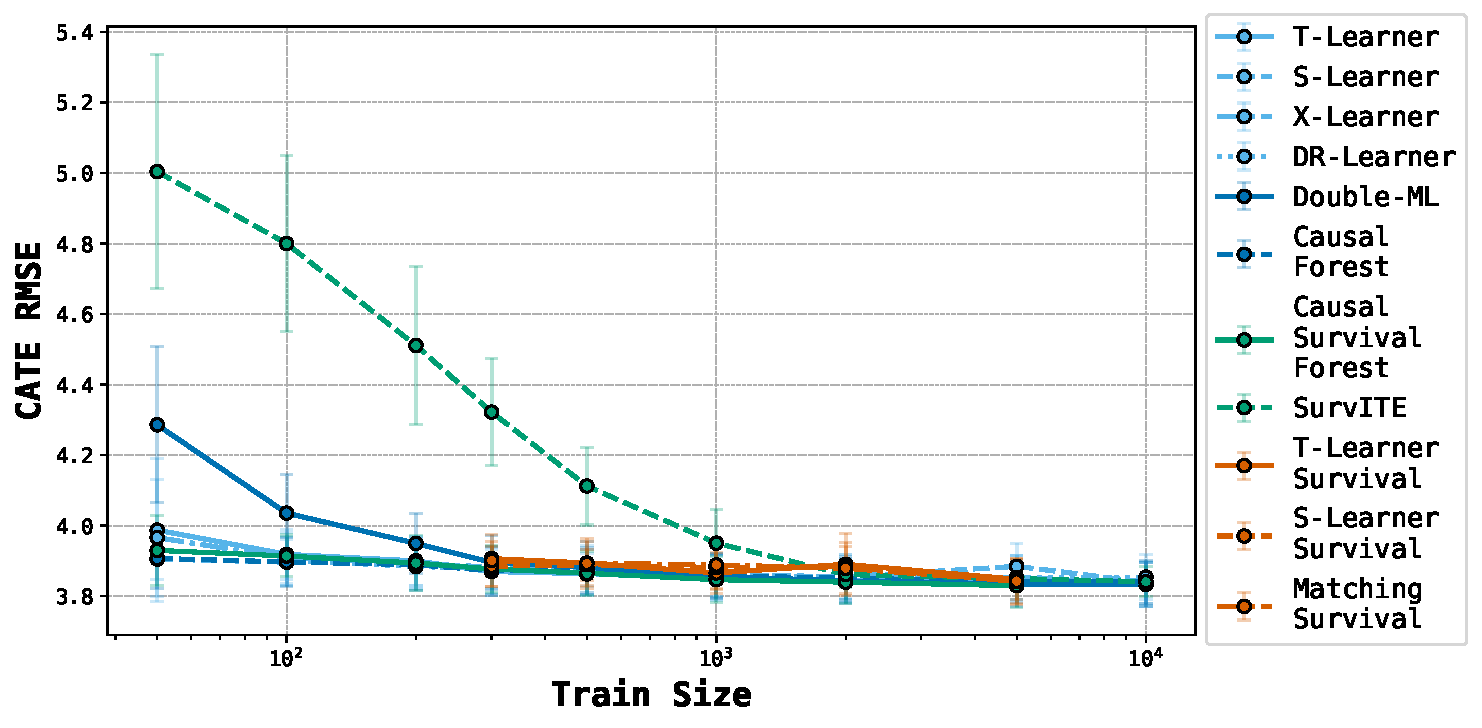
\includegraphics[width=\linewidth]{Appendices/appendix-ch04/images/figure_results_updated/convergence_results/scenario_C_RCT_0_5_convergence.pdf} 
        
    \end{minipage}}
    \hfill
    \subfloat[{RCT: \ChFourGrayCheck (5\%), Ignorability: \ChFourGrayCheck, Positivity: \ChFourGrayCheck, Ign-Censoring: \ChFourGrayCheck}]{\begin{minipage}[t]{0.49\textwidth}
        \centering
        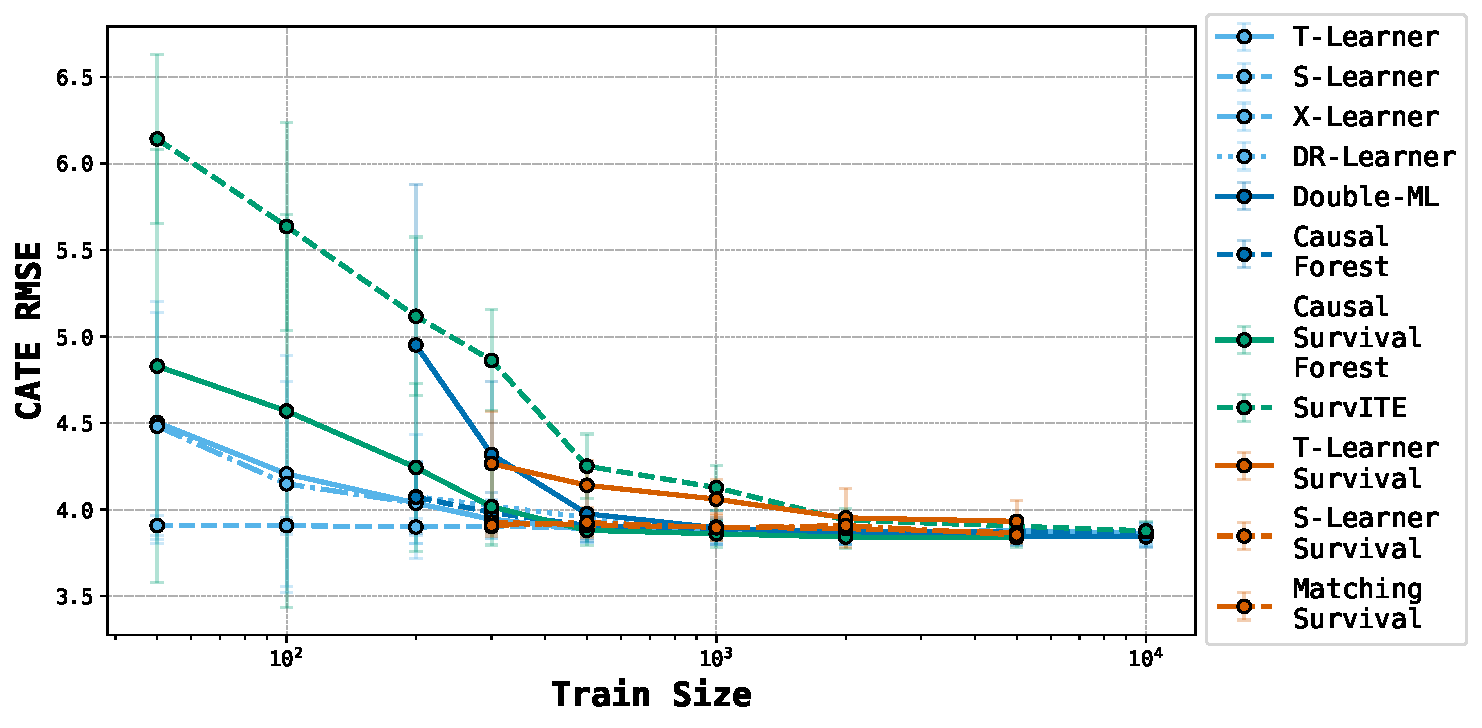
\includegraphics[width=\linewidth]{Appendices/appendix-ch04/images/figure_results_updated/convergence_results/scenario_C_RCT_0_05_convergence.pdf} 
        
    \end{minipage}}

    

    \subfloat[{RCT: \ChFourBlackCross, Ignorability: \ChFourGrayCheck, Positivity: \ChFourGrayCheck, Ignorable Censoring: \ChFourGrayCheck}]{\begin{minipage}[t]{0.49\textwidth}
        \centering
        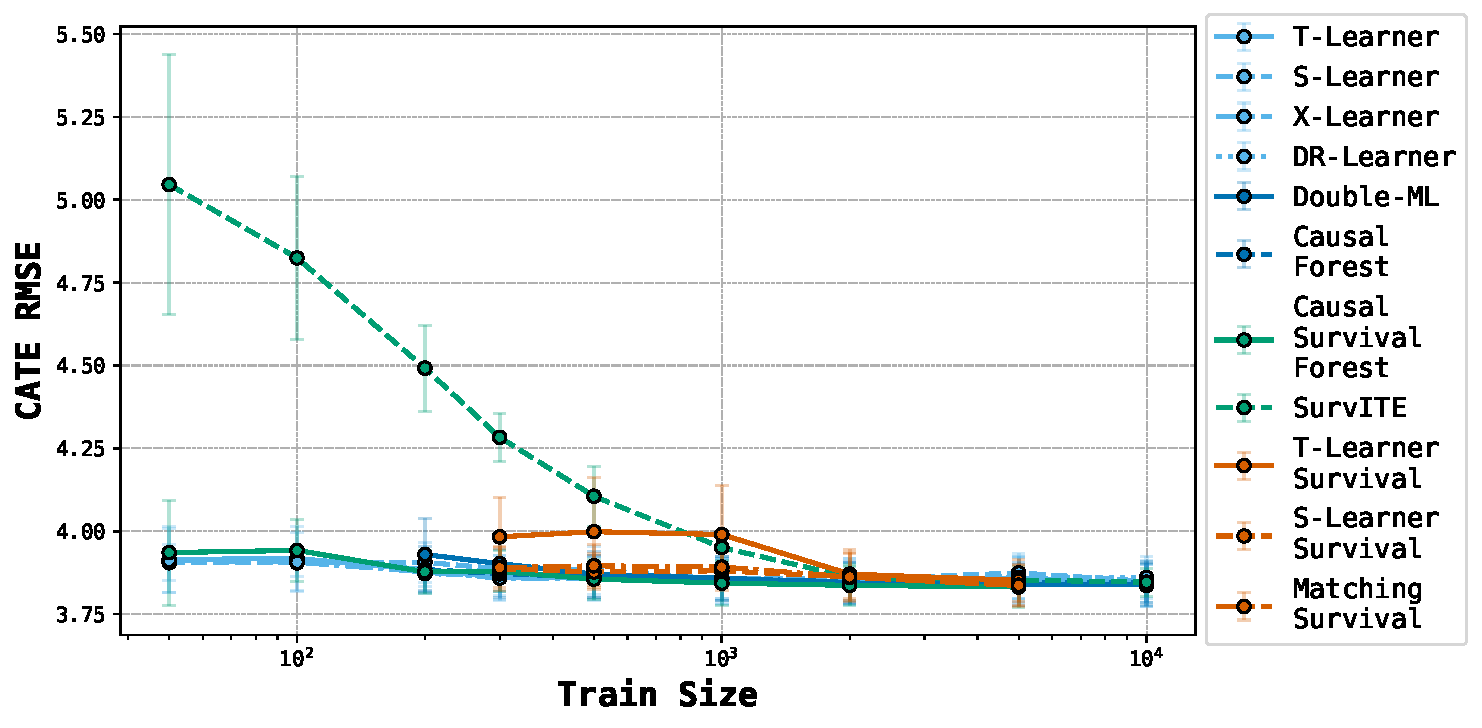
\includegraphics[width=\linewidth]{Appendices/appendix-ch04/images/figure_results_updated/convergence_results/scenario_C_e_X_convergence.pdf} 
        
    \end{minipage}}
    \hfill
    \subfloat[{RCT: \ChFourBlackCross, Ignorability: \ChFourBlackCross, Positivity: \ChFourGrayCheck, Ignorable Censoring: \ChFourGrayCheck}]{\begin{minipage}[t]{0.49\textwidth}
        \centering
        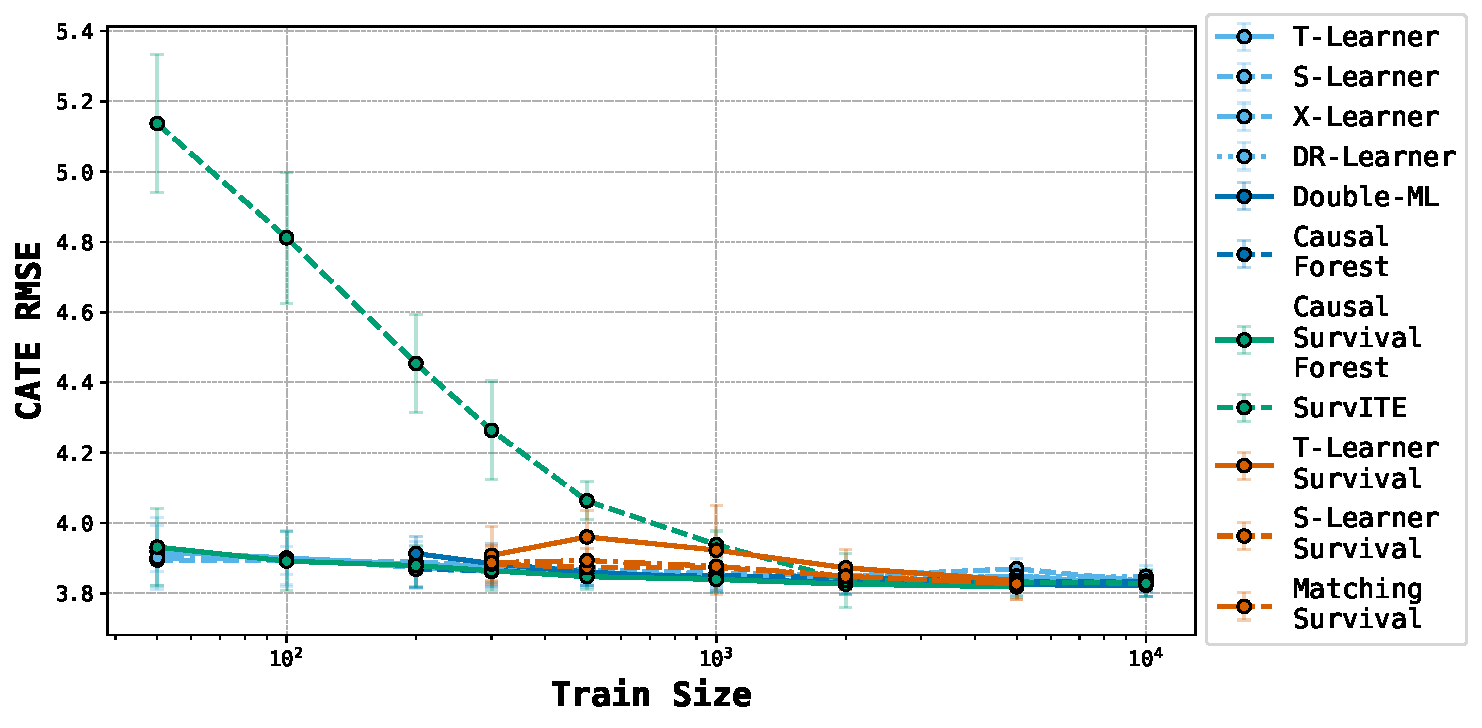
\includegraphics[width=\linewidth]{Appendices/appendix-ch04/images/figure_results_updated/convergence_results/scenario_C_e_X_U_convergence.pdf} 
        
    \end{minipage}}

    

    \subfloat[{RCT: \ChFourBlackCross, Ignorability: \ChFourGrayCheck, Positivity: \ChFourBlackCross, Ignorable Censoring: \ChFourGrayCheck}]{\begin{minipage}[t]{0.49\textwidth}
        \centering
        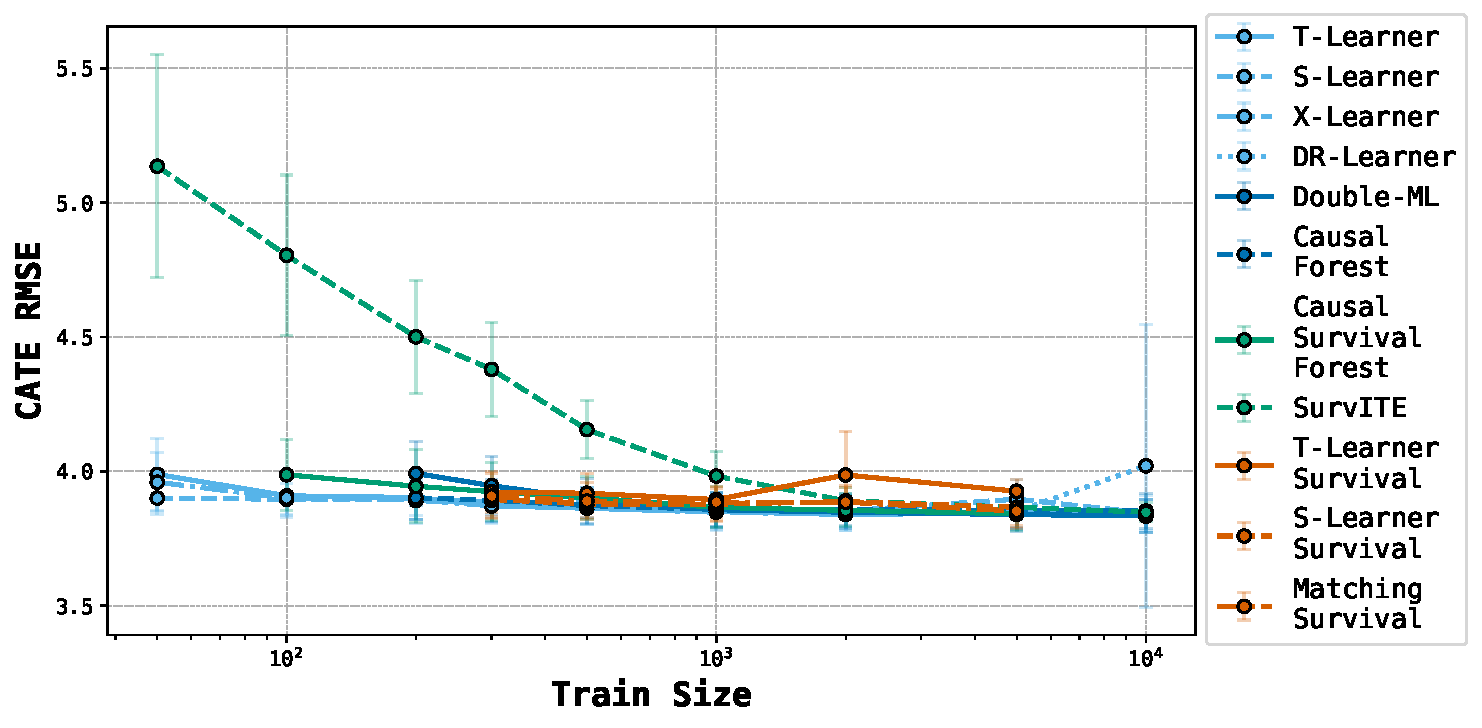
\includegraphics[width=\linewidth]{Appendices/appendix-ch04/images/figure_results_updated/convergence_results/scenario_C_e_X_no_overlap_convergence.pdf} 
        
    \end{minipage}}
    \hfill
    \subfloat[{RCT: \ChFourBlackCross, Ignorability: \ChFourGrayCheck, Positivity: \ChFourGrayCheck, Ignorable Censoring: \ChFourBlackCross}]{\begin{minipage}[t]{0.49\textwidth}
        \centering
        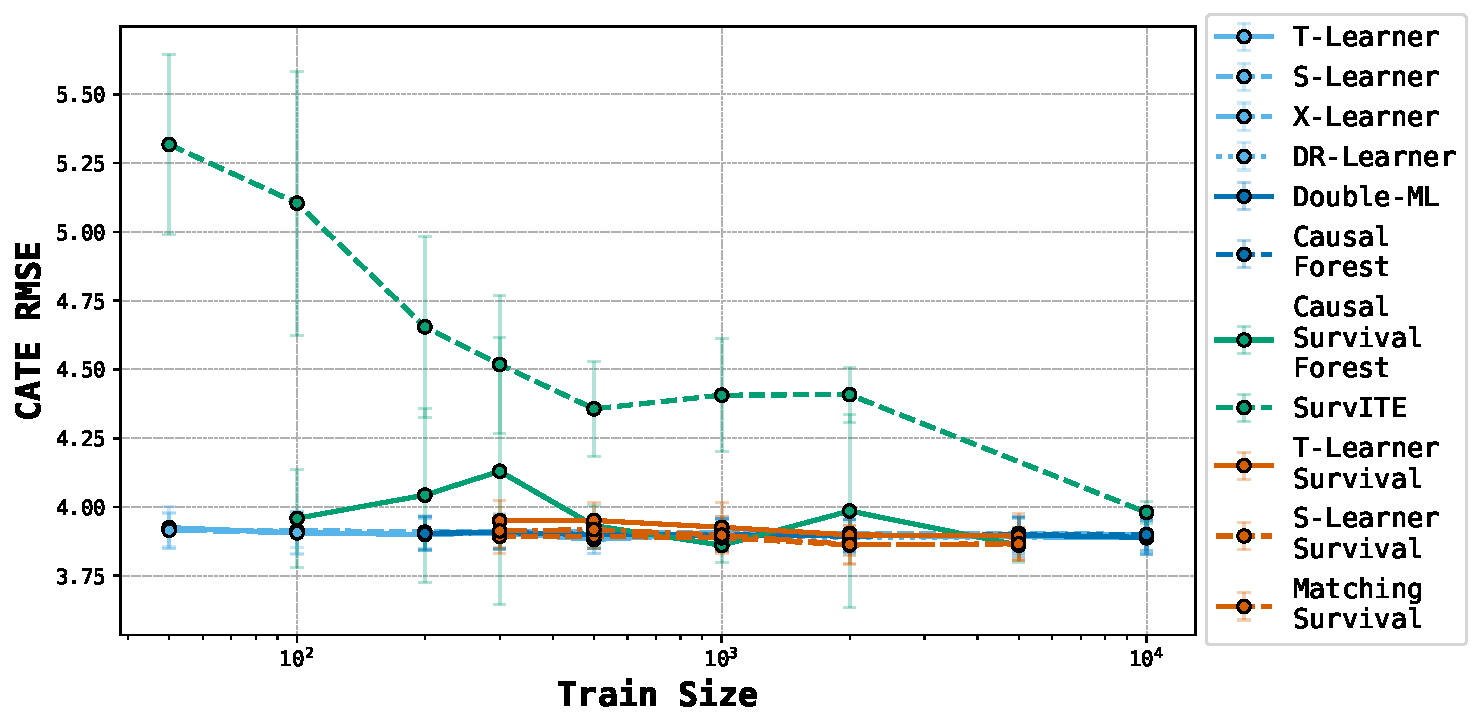
\includegraphics[width=\linewidth]{Appendices/appendix-ch04/images/figure_results_updated/convergence_results/scenario_C_e_X_info_censor_convergence.pdf} 
        
    \end{minipage}}

    

    \subfloat[{RCT: \ChFourBlackCross, Ignorability: \ChFourBlackCross, Positivity: \ChFourGrayCheck, Ignorable Censoring: \ChFourBlackCross}]{\begin{minipage}[t]{0.49\textwidth}
        \centering
        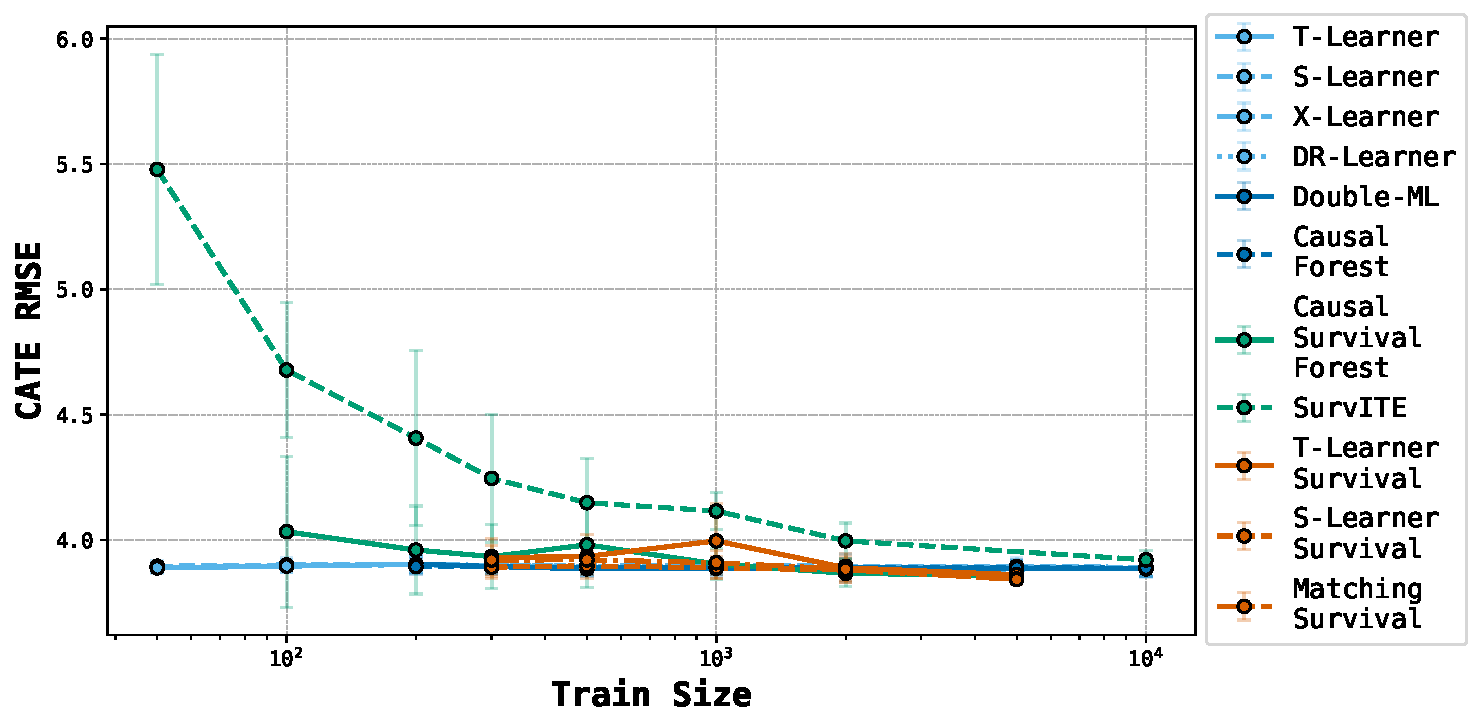
\includegraphics[width=\linewidth]{Appendices/appendix-ch04/images/figure_results_updated/convergence_results/scenario_C_e_X_U_info_censor_convergence.pdf} 
        
    \end{minipage}}
    \hfill
    \subfloat[{RCT: \ChFourBlackCross, Ignorability: \ChFourGrayCheck, Positivity: \ChFourBlackCross, Ignorable Censoring: \ChFourBlackCross}]{\begin{minipage}[t]{0.49\textwidth}
        \centering
        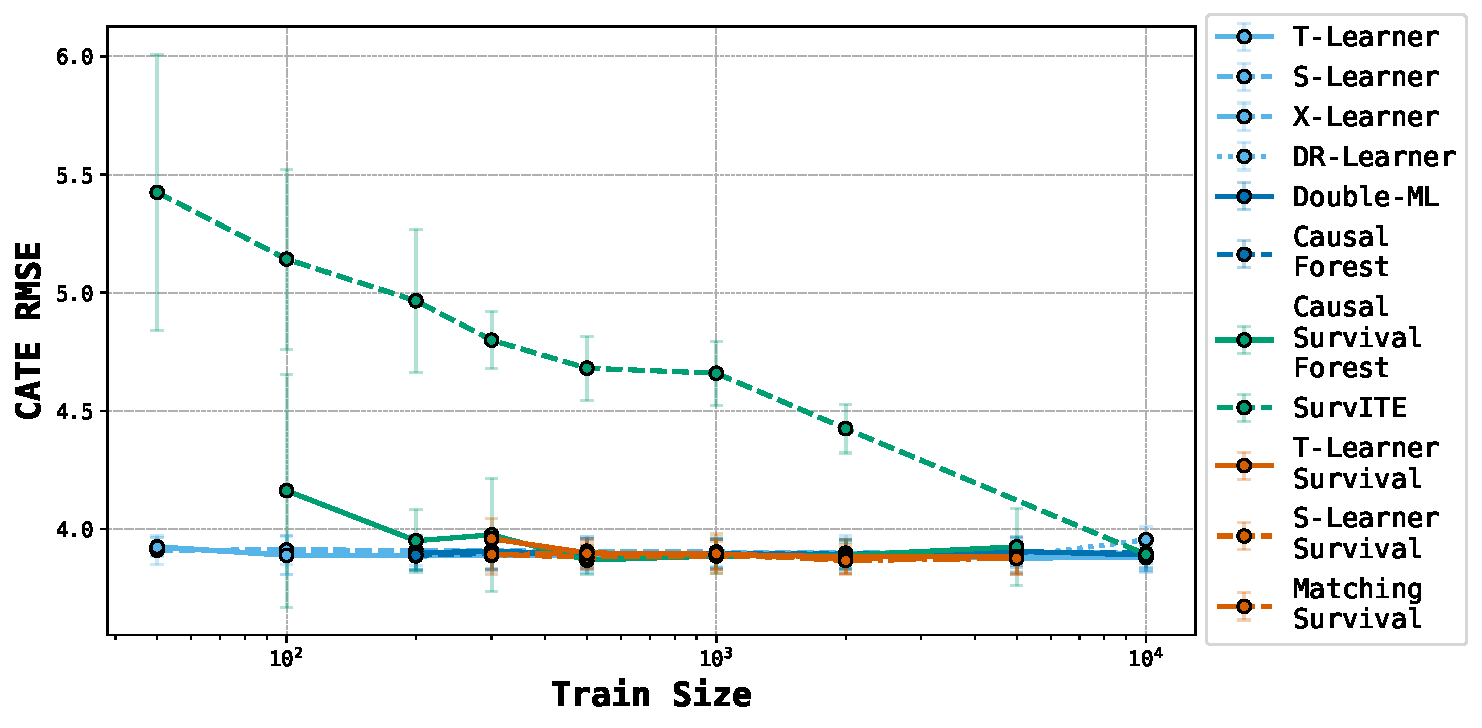
\includegraphics[width=\linewidth]{Appendices/appendix-ch04/images/figure_results_updated/convergence_results/scenario_C_e_X_no_overlap_info_censor_convergence.pdf} 
        
    \end{minipage}}

    \end{minipage}%
    }
    
    
    
}
\end{figure}




%%%%%%%%%%%%%%%%%%%%%%%%%%%%%%%%%%%%%%%%%%%%%%%%%%%%%%%%%%%%
%%%%%%%%%%%%%%%%%%%%%%%%%%%%%%%%%%%%%%%%%%%%%%%%%%%%%%%%%%%%
%%%%%%%%%%%%%%%%%%%%%%%%%%%%%%%%%%%%%%%%%%%%%%%%%%%%%%%%%%%%


% !TeX root = ../../../main.tex
\subsection{Semi-Synthetic Datasets: Setup and Additional Results} 
\label{ch04:app:more-semi-syn-data-setup-result}

\ChFourHeadingOnly
\subsubsection{Semi-synthetic datasets setup}
To complement synthetic benchmarks and real-world case studies, we construct semi-synthetic datasets that pair real covariates with simulated treatment assignment and survival outcomes.
This strategy preserves realistic covariate distributions and correlations while enabling controlled evaluation against known ground-truth CATEs.
We consider two covariate sources: the ACTG HIV trial and MIMIC-IV ICU records.
Table~\ref{ch04:tab:semi-syn-dataset-summary} summarizes dataset sizes, covariate counts, treatment and censoring rates, and whether the treatment-assignment and event-time mechanisms depend on covariates through linear versus non-linear functions; full generative details are provided in Appendix~\ref{ch04:app:actg-semi-dataset} and~\ref{ch04:app:mimic-suite}.
Figure~\ref{ch04:fig:semi-syn-km-curves} shows Kaplan--Meier curves for event and censoring in the treatment and control groups for each semi-synthetic dataset.


% !TeX root = ../../../main.tex
\begin{table}[htbp]
\ChFourFloatContents{ch04:tab:semi-syn-dataset-summary}{\caption{Semi-synthetic datasets overview. The last two columns summarize how treatment assignment and event-time generation depend on covariates. \texttt{linear} indicates dependence through a linear predictor with no quadratic or interaction terms; \texttt{non-linear} includes quadratic and/or interaction terms. \texttt{independent} indicates covariate-independent treatment assignment.}}{
    
     
    \centering
    \setlength{\tabcolsep}{5pt}
    \begin{adjustbox}{max width = \textwidth}
    \begin{tabular}{@{}lcccccc@{}}
        \toprule
        & \makecell{\textbf{Data}\\\textbf{size}} 
        & \makecell{\textbf{No.}\\\textbf{covariates}} 
        & \makecell{\textbf{Treatment}\\\textbf{rate}} 
        & \makecell{\textbf{Censoring.}\\\textbf{rate}} 
        & \makecell{\textbf{Treatment assignment}\\\textbf{mechanism}} 
        & \makecell{\textbf{Event time}\\\textbf{mechanism}} \\
        \midrule
        ACTG & 2,139 & 23 & 56.15\% & 51.19\% & \texttt{linear} & \texttt{non-linear} \\ 
        \addlinespace
        MIMIC-$i$ & 25,170 & 36 & 49.92\% & 88.49\% & \texttt{independent} & \texttt{linear} \\ 
        MIMIC-$ii$ & 25,170 & 36 & 49.92\% & 81.65\% & \texttt{independent} & \texttt{linear} \\ 
        MIMIC-$iii$ & 25,170 & 36 & 49.92\% & 74.10\% & \texttt{independent} & \texttt{linear} \\ 
        MIMIC-$iv$ & 25,170 & 36 & 49.92\% & 66.34\% & \texttt{independent} & \texttt{linear} \\ 
        MIMIC-$v$ & 25,170 & 36 & 49.92\% & 53.35\% & \texttt{independent} & \texttt{linear} \\ 
        \addlinespace
        MIMIC-$vi$ & 25,170 & 36 & 53.54\% & 53.07\% & \texttt{linear} & \texttt{linear} \\ 
        MIMIC-$vii$ & 25,170 & 36 & 54.26\% & 52.66\% & \texttt{linear} & \texttt{non-linear} \\ 
        MIMIC-$viii$ & 25,170 & 36 & 50.94\% & 53.26\% & \texttt{non-linear} & \texttt{linear} \\ 
        MIMIC-$ix$ & 25,170 & 36 & 51.47\% & 52.82\% & \texttt{non-linear} & \texttt{non-linear} \\ 
        \bottomrule
    \end{tabular}
    \end{adjustbox}
    \par
}
\end{table}



% !TeX root = ../../../main.tex
\begin{figure}[htbp]
\ChFourFloatContents{ch04:fig:semi-syn-km-curves}{\caption{(Semi-synthetic datasets) Kaplan-Meier curves. Solid lines show event-time survival under control (blue) and treatment (orange); dotted lines show censoring-time survival for each arm. Each panel reports the empirical censoring rate $c$ and treatment probability $p$.}}{
  \centering
  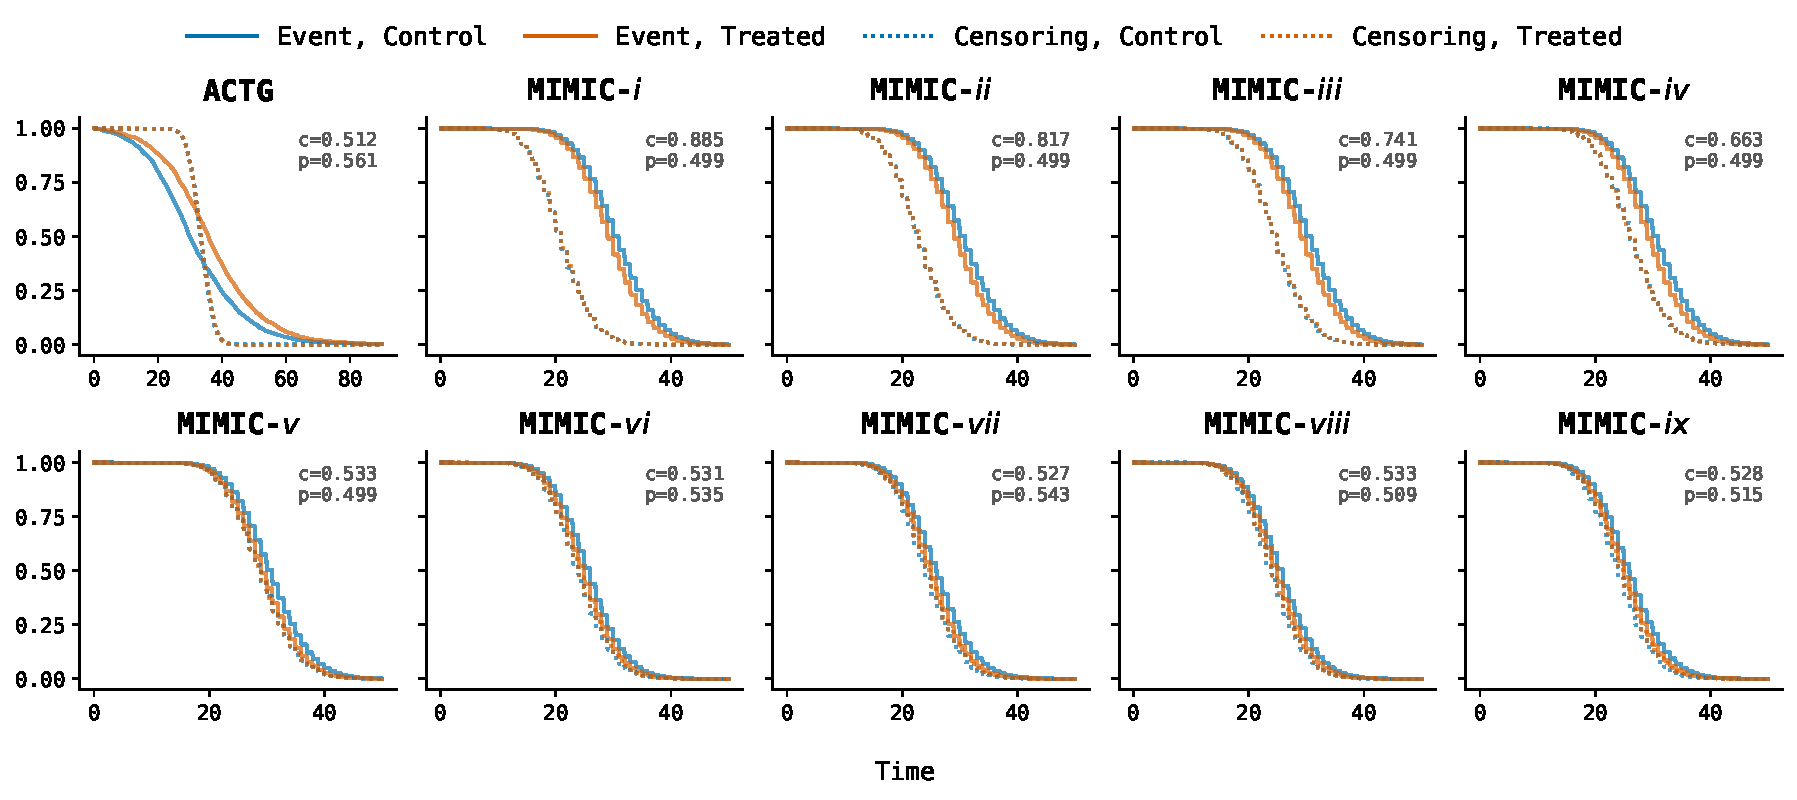
\includegraphics[width=0.98\linewidth]{Appendices/appendix-ch04/images/figure_results_updated/semi-syn-km-curves.pdf} 
   
}
\end{figure}




\subsubsection{ACTG semi-synthetic dataset} \label{ch04:app:actg-semi-dataset}
The ACTG semi-synthetic dataset is derived from the ACTG 175 HIV clinical trial \citep{hammer1996atrial}, which contains 23 baseline covariates.
Following the construction procedure of \citet{chapfuwa2021enabling}, we simulate covariate-dependent treatment assignment and generate event times from a Gompertz--Cox model with an AFT-style censoring mechanism.
This dataset exhibits realistic treatment imbalance and moderate censoring ($\sim$51\%), providing a clinically grounded benchmark with preserved trial covariate structure.

More concretely, following \citet{chapfuwa2021enabling}, we generate: 
$$X = \text{ACTG covariates}$$
$$P(A=1|X=x) = \frac{1}{b} \times \left(a + \sigma\left( \eta ({\rm AGE} - \mu_{\rm AGE} + {\rm CD40} - \mu_{\rm CD40}) \right) \right)$$
$$ U  \sim {\rm Uniform} (0, 1 )$$
$$T_A  =  \frac{1}{\alpha_A} \log \left[1 - \frac{\alpha_A \log U}{ \lambda_A  \exp\left( x ^T  \beta_A\right)  }  \right]$$
$$\log C  \sim {\rm Normal} (\mu_c, \sigma_c^2)$$
$$Y = \min(T_A, C)$$
where $\sigma(\cdot)$ is the sigmoid function, $\{ \beta_A, \alpha_A, \lambda_A, b, a, \eta, \mu_c, \sigma_c \}$ are hyper-parameters taken to be the same as described at \url{https://github.com/paidamoyo/counterfactual_survival_analysis} and $\{\mu_{\rm AGE},  \mu_{\rm CD40}\}$ are the means for age and CD40 respectively.


\subsubsection{MIMIC semi-synthetic datasets}
\label{ch04:app:mimic-suite}
{\raggedright We construct a suite of nine semi-synthetic datasets derived from MIMIC-IV ICU records~\citep{johnson2023mimic}. All variants share the same covariates and sample size, and differ only in the treatment-assignment and event/censoring mechanisms. The suite is organized into two complementary subsets: (1) \emph{independent assignment with varying censoring severity} (MIMIC-$i$--$v$), which isolates robustness to censoring under randomized treatment; and (2) \emph{confounded assignment with varying functional form} (MIMIC-$vi$--$ix$), which evaluates robustness to observed confounding and to non-linear (interaction-based) event and censoring mechanisms while keeping covariates fixed.\par}


We extract 36 covariates spanning laboratory test abnormalities (e.g., creatinine, glucose, hemoglobin), demographic features (e.g., age, sex, race, marital status), and admission descriptors (e.g., admission type, recurrent admissions, night admission).
Table~\ref{ch04:tab:mimic-covariates} summarizes covariate statistics; Table~\ref{ch04:tab:mimic-demographics} reports demographic and categorical distributions; and Figure~\ref{ch04:fig:mimic_corr} shows correlations among covariates.



% !TeX root = ../../../main.tex
\begin{table}[htbp]
\ChFourFloatContents{ch04:tab:mimic-covariates}{\caption{Summary statistics of MIMIC semi-synthetic covariates. Reported values are mean $\pm$ standard deviation. 
    Physiological covariates are coded as indicators for abnormal values where mean reflects prevalence of abnormality.}}{
    

    
    \centering
    \begin{adjustbox}{max width = 0.7\textwidth}
    \begin{tabular}{
        l
        >{\centering\arraybackslash}p{0.18\textwidth}
        l
        >{\centering\arraybackslash}p{0.18\textwidth}
    }
    
    \toprule
    \textbf{Covariate} & Mean $\pm$ Std & \textbf{Covariate} & Mean $\pm$ Std \\
    \midrule
    Sodium & 0.12 $\pm$ 0.32 & Admission age & 61.39 $\pm$ 17.97 \\
    Potassium & 0.08 $\pm$ 0.28 & Sex:Male & 0.51 $\pm$ 0.50 \\
    Chloride & 0.19 $\pm$ 0.39 & Race:White & 0.70 $\pm$ 0.46 \\
    Bicarbonate & 0.24 $\pm$ 0.43 & Race:Black & 0.14 $\pm$ 0.35 \\
    Anion gap & 0.09 $\pm$ 0.29 & Race:Hispanic & 0.05 $\pm$ 0.22 \\
    Creatinine & 0.28 $\pm$ 0.45 & Race:Other & 0.07 $\pm$ 0.25 \\
    Urea nitrogen & 0.40 $\pm$ 0.49 & Insurance:Medicare & 0.42 $\pm$ 0.49 \\
    Glucose & 0.65 $\pm$ 0.48 & Insurance:Other & 0.52 $\pm$ 0.50 \\
    Calcium total & 0.29 $\pm$ 0.45 & Marital status:Married & 0.45 $\pm$ 0.50 \\
    Magnesium & 0.09 $\pm$ 0.28 & Marital status:Single & 0.33 $\pm$ 0.47 \\
    Phosphate & 0.28 $\pm$ 0.45 & Marital status:Widowed & 0.14 $\pm$ 0.34 \\
    Hemoglobin & 0.73 $\pm$ 0.44 & Direct emergency:Yes & 0.11 $\pm$ 0.31 \\
    Hematocrit & 0.69 $\pm$ 0.46 & Night admission:Yes & 0.54 $\pm$ 0.50 \\
    MCV & 0.20 $\pm$ 0.40 & \makecell{Previous admission\\this month: Yes} & 0.08 $\pm$ 0.27 \\
    MCH & 0.26 $\pm$ 0.44 & Admissions number:2 & 0.16 $\pm$ 0.37 \\
    MCHC & 0.31 $\pm$ 0.46 & Admissions number:3+ & 0.22 $\pm$ 0.42 \\
    Platelet count & 0.29 $\pm$ 0.45 & & \\
    RDW & 0.29 $\pm$ 0.45 & & \\
    White blood cells & 0.40 $\pm$ 0.49 & & \\
    Red blood cells & 0.76 $\pm$ 0.43 & & \\
    \bottomrule
    \end{tabular}
    \end{adjustbox}
}
\end{table}




% !TeX root = ../../../main.tex
\begin{table}[htbp]
\ChFourFloatContents{ch04:tab:mimic-demographics}{\caption{Demographic and categorical distributions in MIMIC semi-synthetic datasets. Reported values are proportions.}}{
  
  
  \centering \small
  \begin{minipage}[t]{0.48\textwidth}
    \centering
    \textbf{Demographics}\par
    \begin{tabular}{lc}
      \toprule
      Variable & Proportion \\
      \midrule
      \textbf{Sex} & \\
      Male   & 0.512 \\
      Female & 0.488 \\
      \addlinespace
      \textbf{Race} & \\
      White    & 0.699 \\
      Black    & 0.141 \\
      Other    & 0.066 \\
      Hispanic & 0.053 \\
      Asian    & 0.041 \\
      \addlinespace
      \textbf{Insurance} & \\
      Other    & 0.522 \\
      Medicare & 0.421 \\
      Medicaid & 0.057 \\
      \addlinespace
      \textbf{Marital status} & \\
      Married  & 0.449 \\
      Single   & 0.334 \\
      Widowed  & 0.136 \\
      Divorced & 0.081 \\
      \bottomrule
    \end{tabular}
  \end{minipage}
  \hfill
  \begin{minipage}[t]{0.48\textwidth}
    \centering
    \textbf{Admission-related}\par
    \begin{tabular}{lc}
      \toprule
      Variable & Proportion \\
      \midrule
      \textbf{Direct emergency} & \\
      Yes & 0.110 \\
      No  & 0.890 \\
      \addlinespace
      \textbf{Night admission} & \\
      Yes & 0.539 \\
      No  & 0.461 \\
      \addlinespace
      \textbf{\makecell{Previous admission\\this month}} & \\
      Yes & 0.081 \\
      No  & 0.919 \\
      \addlinespace
      \textbf{Admissions number} & \\
      1   & 0.615 \\
      2   & 0.164 \\
      3+  & 0.222 \\
      \bottomrule
    \end{tabular}
  \end{minipage}
}
\end{table}



% !TeX root = ../../../main.tex
\begin{figure}[htbp]
\ChFourFloatContents{ch04:fig:mimic_corr}{\caption{Correlation heatmap of the 36 semi-synthetic MIMIC covariates. Variables include demographic features, admission descriptors, insurance and marital status indicators, and laboratory measurements. Most correlations are weak to moderate, with stronger dependencies visible among related laboratory values (e.g., hematocrit, hemoglobin, and red blood cell count).}}{
  \centering
  
  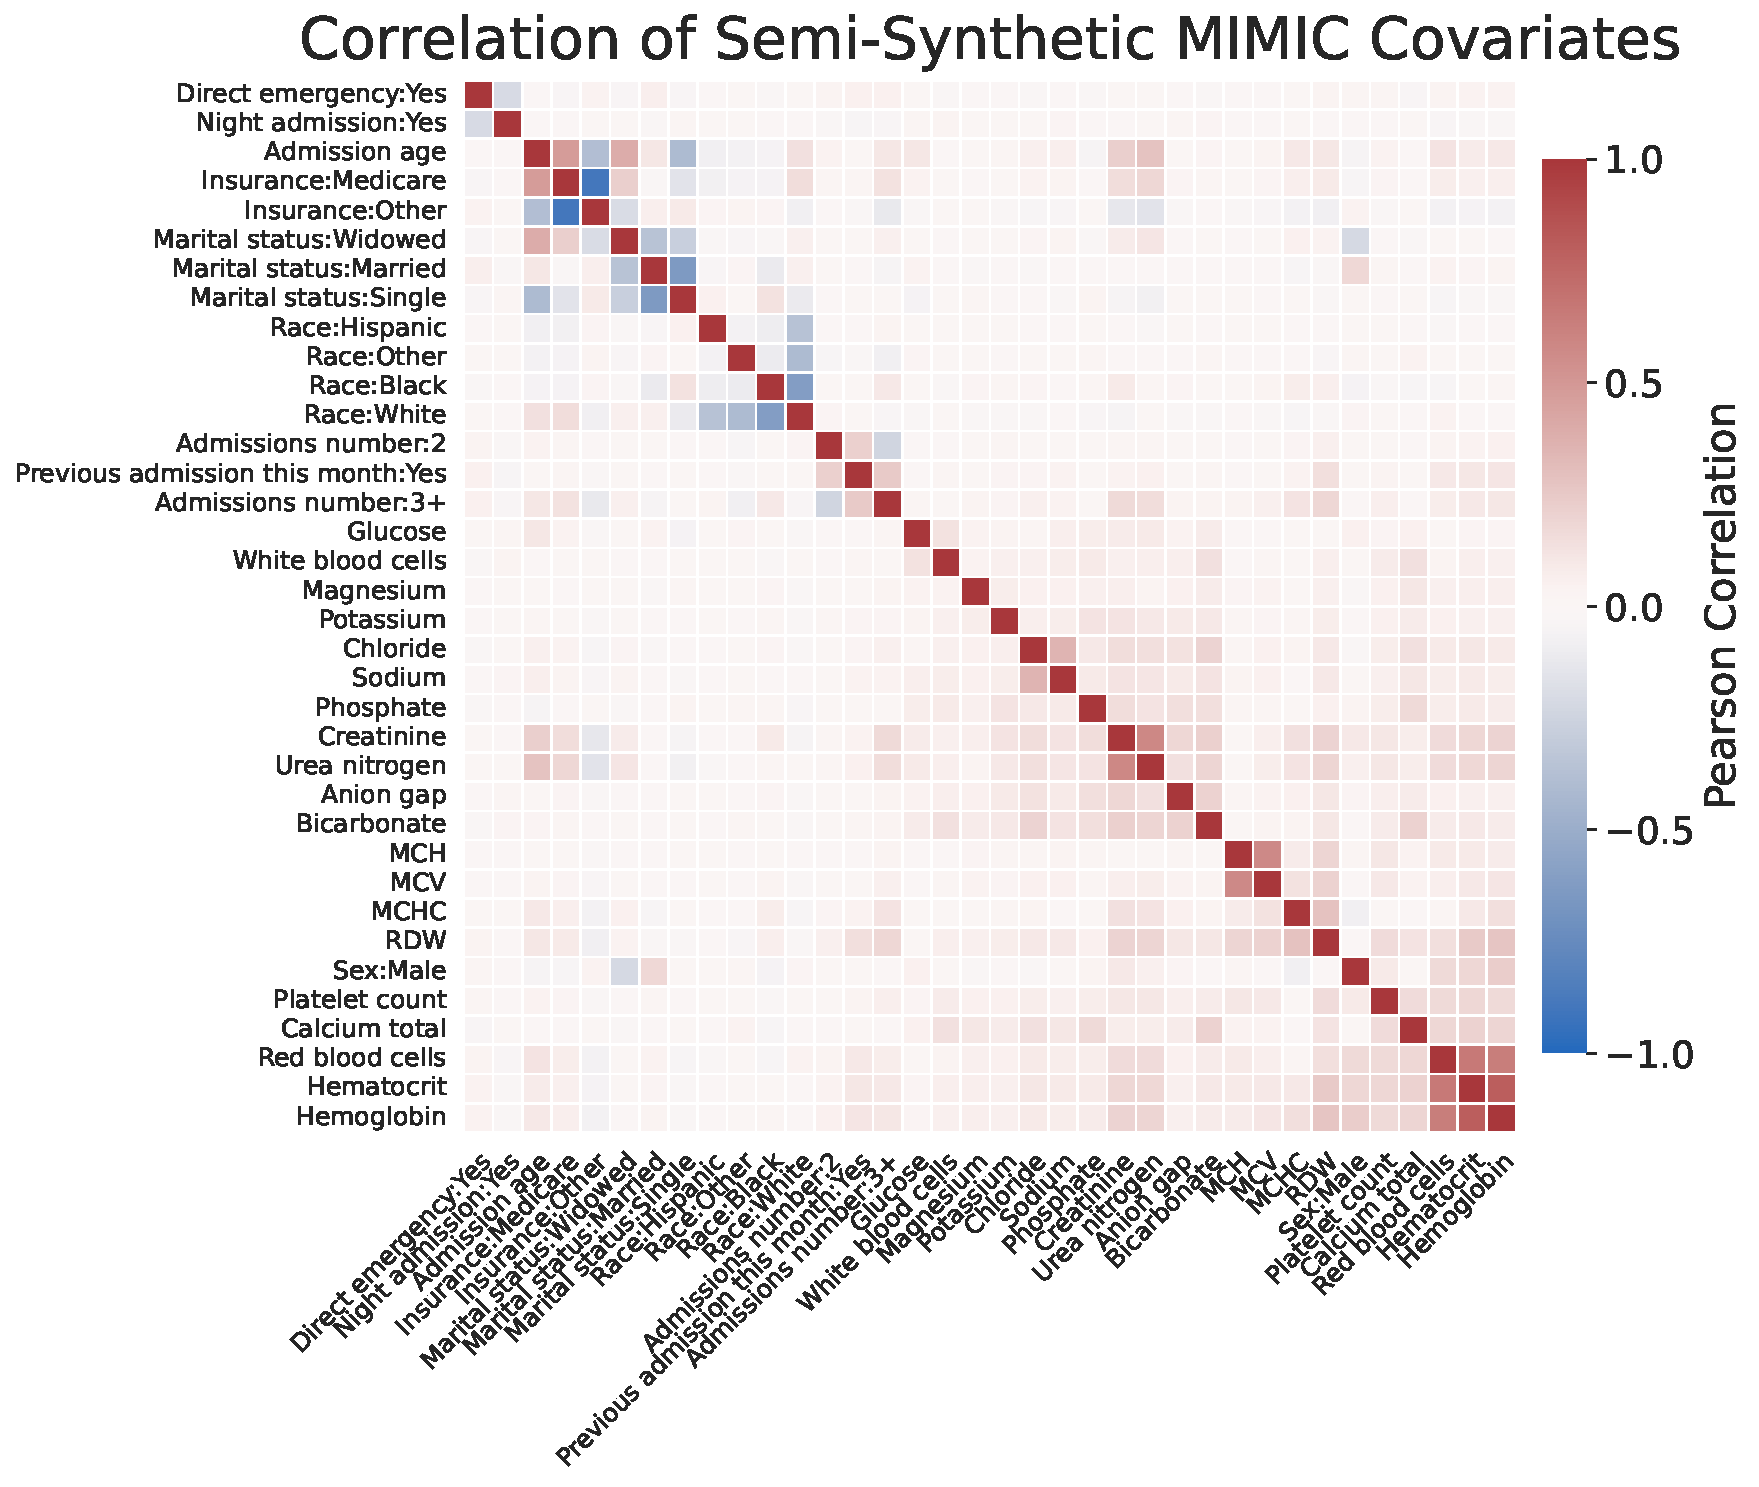
\includegraphics[width=.8\linewidth]{Appendices/appendix-ch04/images/figure_results_updated/corr_heatmap_mimic.pdf}
   
  
}
\end{figure}


We now introduce some shared notation in all of the MIMIC semi-synthetic datasets.
Let $X_{1:5}$ denote the first five binary covariates corresponding to abnormal laboratory values
(\textit{Anion gap}, \textit{Bicarbonate}, \textit{Calcium total}, \textit{Chloride}, \textit{Creatinine}),
and let $X_{36}$ denote the standardized \textit{Admission age}.
We define the abnormal-lab burden as
\[
S = \sum_{j=1}^{5} X_j.
\]
Across all MIMIC variants, we generate potential event times $T(0),T(1)$ and a censoring time $C$, and observe
\[
T = W T(1) + (1-W)T(0),\quad Y=\min(T,C),\quad \delta=\ChFourInd\{T\le C\}.
\]


\paragraph{Independent-assignment, varying censoring (MIMIC-$i$--$v$)}
\label{ch04:app:mimic-i-v}
This subset follows the event-time construction of~\citet{meir2025heterogeneous} and varies censoring severity to span moderate to extreme censoring regimes.

\ChFourParagraph{Treatment assignment.}
Treatment is assigned independently of covariates:
\[
W \sim \mathrm{Bernoulli}(0.5),
\]
yielding balanced treatment groups with $W \perp X$.

\ChFourParagraph{Potential outcomes.}
Potential event times are Poisson with means depending on $S$ and $X_{36}$:
\begin{align*}
    T(0) &\sim \mathrm{Poisson}\!\left(30 + 0.75 S + 0.75 X_{36}\right), \\
    T(1) &\sim \mathrm{Poisson}\!\left(30 + 0.75 X_{36} - 0.45\right).
\end{align*}
We define the conditional average treatment effect (CATE) as $\tau(x)=\mathbb{E}[T(1)-T(0)\mid X=x]$ and record unit-level ground truth CATE as $T(1)-T(0)$.

\ChFourParagraph{Censoring.}
Censoring is independent and varies across dataset variants:
\[
C \sim \mathrm{Poisson}(\lambda_c),
\]
where $\lambda_c \in \{21, 23, 24.7, 26.5, 29\}$ controls censoring severity for MIMIC-$i$--$v$, yielding censoring rates from approximately 53\% to 88\%.



\paragraph{Confounded assignment, varying functional form (MIMIC-$vi$--$ix$)}
\label{ch04:app:mimic-vi-ix}
This subset reuses the same covariate backbone but introduces covariate-dependent treatment assignment (observed confounding) with a propensity score and varies whether the event-time and censoring mechanisms are linear or non-linear in covariates.
The four variants correspond to the following combinations:
\begin{itemize}
    \item MIMIC-$vi$: Propensity score=\texttt{linear}, event/censoring time=\texttt{linear};
    \item MIMIC-$vii$: Propensity score=\texttt{linear}, event/censoring time=\texttt{non-linear};
    \item MIMIC-$viii$: Propensity score=\texttt{non-linear}, event/censoring time=\texttt{linear};
    \item MIMIC-$ix$: Propensity score=\texttt{non-linear}, event/censoring time=\texttt{non-linear}.
\end{itemize}

\ChFourParagraph{Covariate-dependent treatment assignment (propensity score).}
We consider two propensity-score families:
\begin{itemize}
    \item \textbf{Linear (no interactions or quadratic terms).}
    \begin{align*}
        \eta(x) &= \alpha_0+\alpha_1 X_{36}+\alpha_2 S,\\
        e(x) &= \Pr(W=1\mid X=x)=\sigma(\eta(x)),\quad
        W\mid X \sim \mathrm{Bernoulli}(e(X)),
    \end{align*}
    with $(a_0,a_1,a_2)=(-0.25,\,0.8,\,0.4)$;
    \item \textbf{Non-linear (quadratic + interaction).}
    \begin{align*}
        \eta(x) &= \beta_0 + \beta_1 X_{36} + \beta_2 S + \beta_3 X_{36}^2 + \beta_4 X_{36} S,\\
        e(x) &= \Pr(W=1\mid X=x)=\sigma(\eta(x)),\quad
        W\mid X \sim \mathrm{Bernoulli}(e(X)),
    \end{align*}
    with $(b_0,b_1,b_2,b_3,b_4)=(-0.2,\,0.8,\,0.4,\,-0.3,\,0.5)$.
\end{itemize}
where $\sigma(\cdot)$ is the sigmoid function.
We clip $e(x)$ into $[0.05,0.95]$ to avoid near-deterministic treatment assignment and preserve overlap.
Note that the coefficients are chosen (by checking the realized $\mathbb{E}[W]$) so that the treatment rate remains close to $0.5$ while inducing confounding through $X_{36}$ and $S$.


\ChFourParagraph{Event-time and censoring mechanisms.}
Potential outcomes and censoring are defined through Poisson means with an identity link and are clipped below at $1$ to ensure positivity.

\begin{itemize}
    \item \textbf{Linear (no interactions or quadratic terms).}
    \begin{align*}
        \mu_0(x) &= \psi_{00} + \psi_{01} S + \psi_{02} X_{36}, \\
        \mu_1(x) &= \psi_{10} + \psi_{11} S + \psi_{12} X_{36},
    \end{align*}
    with $(\psi_{00},\psi_{01},\psi_{02})=(25.0,\,0.75,\,0.75)$ and $(\psi_{10},\psi_{11},\psi_{12})=(25.0,\,0.0,\,0.75)$, and
    \begin{align*}
        T(0) &\sim \mathrm{Poisson}(\max\{1,\mu_0(X)\}),\quad
        T(1) \sim \mathrm{Poisson}(\max\{1,\mu_1(X)\}).
    \end{align*}
    Censoring is
    \begin{align*}
        \lambda_c(x) &= \omega_0 + \omega_1 S + \omega_2 X_{36},\quad
        C \sim \mathrm{Poisson}(\max\{1,\lambda_c(X)\}).
    \end{align*}
    with $(\omega_0,\omega_1,\omega_2)=(24.0,\,0.2,\,0.2)$.

    \item \textbf{Non-linear (quadratic + interaction).}
    \begin{align*}
        \mu_0(x) &= \psi_{00} + \psi_{01} S + \psi_{02} X_{36} + \psi_{03} X_{36}^2 + \psi_{04} X_{36} S, \\
        \mu_1(x) &= \psi_{10} + \psi_{11} S + \psi_{12} X_{36} + \psi_{13} X_{36}^2 + \psi_{14} X_{36} S,
    \end{align*}
    with $(\psi_{00},\psi_{01},\psi_{02},\psi_{03},\psi_{04})=(25.0,\,0.75,\,0.75,\,0.3,\,0.5)$ and $(\psi_{10},\psi_{11},\psi_{12},\psi_{13},\psi_{14})=(25.0,\,0.0,\,0.75,\,0.2,\,0.4)$, and
    \begin{align*}
        T(0) &\sim \mathrm{Poisson}(\max\{1,\mu_0(X)\}),\quad
        T(1) \sim \mathrm{Poisson}(\max\{1,\mu_1(X)\}).
    \end{align*}
    Censoring is
    \begin{align*}
        \lambda_c(x) &= \omega_0 + \omega_1 S + \omega_2 X_{36} + \omega_3 X_{36}^2 + \omega_4 X_{36} S,\\
        C &\sim \mathrm{Poisson}(\max\{1,\lambda_c(X)\}).
    \end{align*}
    with $(\omega_0,\omega_1,\omega_2,\omega_3,\omega_4)=(24.0,\,0.2,\,0.2,\,0.3,\,0.4)$
\end{itemize}
These mechanisms allow survival outcomes and censoring to vary non-linearly with baseline severity (lab abnormalities) and age, thereby creating heterogeneous and more realistic treatment effects.

\ChFourParagraph{Fixed-horizon survival probabilities.}
Because event times are Poisson-distributed, the conditional survival probability for arm $w\in\{0,1\}$ at discrete horizon $t$ is
\[
S_w(t\mid X)=\Pr(T(w)>t\mid X)=1-\sum_{k=0}^{\lfloor t\rfloor}\frac{e^{-\mu_w(X)}\mu_w(X)^k}{k!}.
\]
For each dataset, we compute unit-level ground-truth survival probabilities at horizons corresponding to the empirical 25th, 50th, and 75th percentiles of the realized event-time distribution, and use these when evaluating survival-probability CATE estimands.



Across all MIMIC variants, the sample size is $N=25{,}170$ and the covariate distributions in Tables~\ref{ch04:tab:mimic-covariates} and~\ref{ch04:tab:mimic-demographics} are identical.
The subset MIMIC-$i$--$v$ spans censoring rates from approximately 53\% to 88\% under covariate-independent treatment assignment ($\Pr(W{=}1)\approx 0.5$), isolating the effect of censoring severity.
The subset MIMIC-$vi$--$ix$ keeps censoring moderate (around 53\% in our instantiation) while introducing covariate-dependent treatment assignment and varying whether event-time and censoring mechanisms are linear or non-linear in covariates, providing complementary stress tests for both confounding and misspecified or non-linear hazard/censoring relationships.


\subsubsection{Semi-synthetic results: full MIMIC suite and additional estimands}
\label{ch04:app:other-estimand-result}

This section extends the semi-synthetic evaluation in Section~\ref{ch04:sec:semi-syn-data-experiment}.
First, we complete coverage of the full MIMIC semi-synthetic suite by reporting RMST-based CATE RMSE on MIMIC-$vi$--$ix$ under the same primary estimand used in the main paper (RMST evaluated at the maximum observed time $T_{\max}$).
Second, we report results for additional estimands that probe time-horizon sensitivity: horizon-specific survival-probability CATEs and RMST evaluated at a shorter horizon (the median event time $T_{\text{med}}$).


\paragraph{Primary estimand: RMST at $T_{\max}$ (full MIMIC suite)}
\label{ch04:app:semi-syn-rmst-tmax}

The main paper reports RMST-based CATE RMSE on ACTG and the censoring-severity subset MIMIC-$i$--$v$ (Table~\ref{ch04:tab:semi-syn-cate-rmse}).
Table~\ref{ch04:tab:mimic-vi-ix-results} reports CATE RMSE on MIMIC-$vi$--$ix$ using the same estimand as in the main paper: RMST evaluated at the maximum observed time in each dataset.
These variants reuse the same covariates as MIMIC-$i$--$v$ but introduce covariate-dependent treatment assignment and/or non-linear event-time and censoring mechanisms (Appendix~\ref{ch04:app:mimic-vi-ix}).
Across MIMIC-$i$--$ix$, mean RMSE values typically lie in a narrow band, so practical differences are often reflected more strongly in stability (variance across repetitions) than in average error.

\ChFourParagraph{Dataset-dependent performance patterns.}
The ACTG dataset (Table~\ref{ch04:tab:semi-syn-cate-rmse}) exhibits clearer separation among methods, whereas the MIMIC variants (Tables~\ref{ch04:tab:semi-syn-cate-rmse} and~\ref{ch04:tab:mimic-vi-ix-results}) show substantially tighter clustering.
This reinforces that method rankings can depend on covariate structure and data-generating mechanisms: approaches that perform well in trial-like settings (ACTG) need not be the strongest in high-dimensional EHR-like settings (MIMIC), and vice versa.

\ChFourParagraph{Censoring-gradient and stability under MIMIC-$i$--$v$.}
The censoring sweep MIMIC-$i$--$v$ (53\%--88\% censoring) provides a granular view of censoring sensitivity.
Several methods maintain stable mean RMSE as censoring increases, but standard deviation can change markedly for some learners under extreme censoring (Table~\ref{ch04:tab:semi-syn-cate-rmse}).
As a result, stability considerations (e.g., standard deviation across repeats) can be as important as mean RMSE when operating in highly censored regimes typical of EHR studies.

\ChFourParagraph{Robustness across mechanism complexity (MIMIC-$vi$--$ix$).}
Moving from MIMIC-$i$--$v$ to the mechanism-complexity subset MIMIC-$vi$--$ix$ does not qualitatively change the overall picture: multiple methods remain competitive and the top-performing group (Causal Survival Forests and S-Learner-Survival) is often tightly clustered (Table~\ref{ch04:tab:mimic-vi-ix-results}).
This suggests that the primary conclusions drawn from MIMIC-$i$--$v$ are not driven solely by covariate-independent treatment assignment; rather, they persist under observed confounding and non-linear outcome/censoring mechanisms within the same covariate support.



% !TeX root = ../../../main.tex
\begin{table}[htbp]
\ChFourFloatContents{ch04:tab:mimic-vi-ix-results}{\caption{CATE RMSE (mean $\pm$ std over 10 repeats) on MIMIC-$vi$--$ix$, using RMST evaluated at the maximum observed time $T_{\max}$ of each dataset as the estimand. Best two methods per dataset are \textbf{bolded}.}}{
    \centering
    
    
    \begin{adjustbox}{max width = 0.8\textwidth}
    \begin{tabular}{lcccc}
    \toprule
        \textbf{Method Family} & \textbf{MIMIC-$vi$} & \textbf{MIMIC-$vii$} & \textbf{MIMIC-$viii$} & \textbf{MIMIC-$ix$} \\ 
    \midrule
    \multicolumn{5}{l}{\textit{Outcome Imputation Methods}} \\
        T-Learner & 7.184 $\pm$ 0.052 & 7.374 $\pm$ 0.067 & 7.220 $\pm$ 0.046 & 7.354 $\pm$ 0.048 \\ 
        S-Learner & 7.176 $\pm$ 0.048 & 7.308 $\pm$ 0.068 & 7.197 $\pm$ 0.049 & 7.275 $\pm$ 0.061 \\ 
        X-Learner & 7.182 $\pm$ 0.053 & 7.318 $\pm$ 0.069 & 7.203 $\pm$ 0.045 & 7.273 $\pm$ 0.044 \\ 
        DR-Learner & 7.145 $\pm$ 0.054 & 7.295 $\pm$ 0.061 & 7.167 $\pm$ 0.046 & 7.263 $\pm$ 0.045 \\ 
        Double-ML & \textbf{7.127 $\pm$ 0.051} & \textbf{7.259 $\pm$ 0.072} & \textbf{7.147 $\pm$ 0.049} & \textbf{7.226 $\pm$ 0.056} \\ 
        Causal Forest & 7.142 $\pm$ 0.052 & 7.288 $\pm$ 0.068 & 7.162 $\pm$ 0.047 & 7.247 $\pm$ 0.043 \\ 
    \addlinespace
    \multicolumn{5}{l}{\textit{Direct-Survival CATE Methods}} \\
        Causal Survival Forests & \textbf{7.123 $\pm$ 0.048} & \textbf{7.281 $\pm$ 0.064} & \textbf{7.149 $\pm$ 0.045} & \textbf{7.227 $\pm$ 0.054} \\ 
        SurvITE & 7.169 $\pm$ 0.042 & 7.286 $\pm$ 0.059 & 7.184 $\pm$ 0.043 & 7.265 $\pm$ 0.055 \\ 
    \addlinespace
    \multicolumn{5}{l}{\textit{Survival Meta-Learners}} \\
        T-Learner-Survival & 7.168 $\pm$ 0.055 & 7.332 $\pm$ 0.071 & 7.188 $\pm$ 0.040 & 7.358 $\pm$ 0.047 \\ 
        S-Learner-Survival & 7.138 $\pm$ 0.048 & 7.285 $\pm$ 0.064 & 7.163 $\pm$ 0.041 & 7.239 $\pm$ 0.055 \\ 
        Matching Survival & 7.163 $\pm$ 0.050 & 7.340 $\pm$ 0.062 & 7.199 $\pm$ 0.043 & 7.297 $\pm$ 0.050 \\ 
    \bottomrule
    \end{tabular}
    \end{adjustbox}
}
\end{table}



\paragraph{Additional estimand: horizon-specific survival-probability CATEs}
\label{ch04:app:surv_prob}

In addition to RMST-based CATEs, we consider treatment effects defined on the survival function at a fixed horizon.
Let $S_i(w;h)=\Pr(T_i(w)>h)$ denote the potential-outcome survival probability for unit $i$ under treatment $w\in\{0,1\}$ at horizon $h$.
In this case, the transformation $y(\cdot)$ in~\ChFourEqref{ch04:eq:cate} is replaced by
\[
y\big(T_i(w)\big) := S_i(w; h).
\]
The corresponding CATE is:
\begin{equation}
    \tau_h(x) := \mathbb{E}\!\left[\, S_i(1; h) - S_i(0; h) \mid X_i=x \right].
\end{equation}
We evaluate $\tau_h(x)$ at three dataset-specific horizons given by the empirical 25th, 50th, and 75th percentiles of the realized event-time distribution.

We evaluate $\tau_h(x)$ at three dataset-specific horizons given by the empirical 25th, 50th, and 75th percentiles of the realized event-time distribution.
We report results for methods that explicitly model conditional survival functions (direct-survival CATE methods and survival meta-learners).
Our outcome-imputation baselines impute event times (or RMST) rather than estimating a full conditional survival curve, and therefore are not included for this estimand.
Tables~\ref{ch04:tab:cate_rmse_prob25}--\ref{ch04:tab:cate_rmse_prob75} summarize RMSE across the MIMIC semi-synthetic datasets for the 25th, 50th, and 75th percentile horizons, respectively. 




% !TeX root = ../../../main.tex
\begin{table}[htbp]
\ChFourFloatContents{ch04:tab:cate_rmse_prob25}{\caption{CATE RMSE (mean $\pm$ std over 10 repeats) on MIMIC semi-synthetic datasets, using survival probability at 25th quantile event time of each dataset as the estimand. Best method per dataset is \textbf{bolded}.}}{
\centering
\footnotesize
\setlength{\tabcolsep}{4pt}


        \par\noindent\begin{adjustbox}{max width=\linewidth}\begin{minipage}[c]{\linewidth}
        \centering
        \begin{adjustbox}{max width=\linewidth}\begin{tabular}{lccccc}
        \toprule
        \textbf{Method Family} & \textbf{MIMIC-$i$} & \textbf{MIMIC-$ii$} & \textbf{MIMIC-$iii$} & \textbf{MIMIC-$iv$} & \textbf{MIMIC-$v$} \\
        \midrule
        \multicolumn{6}{l}{\textit{Direct-Survival CATE Methods}} \\
                Causal Survival Forests & \textbf{0.051 $\pm$ 0.003} & \textbf{0.045 $\pm$ 0.005} & \textbf{0.039 $\pm$ 0.002} & \textbf{0.037 $\pm$ 0.003} & \textbf{0.034 $\pm$ 0.002} \\ 
                SurvITE & 0.066 $\pm$ 0.009 & 0.060 $\pm$ 0.004 & 0.057 $\pm$ 0.008 & 0.055 $\pm$ 0.005 & 0.055 $\pm$ 0.005 \\ 
        \addlinespace
        \multicolumn{6}{l}{\textit{Survival Meta-Learners}} \\
                T-Learner-Survival & 0.083 $\pm$ 0.011 & 0.077 $\pm$ 0.040 & 0.049 $\pm$ 0.008 & 0.047 $\pm$ 0.007 & 0.045 $\pm$ 0.005 \\ 
                S-Learner-Survival & 0.053 $\pm$ 0.006 & 0.050 $\pm$ 0.006 & 0.053 $\pm$ 0.010 & 0.051 $\pm$ 0.004 & 0.046 $\pm$ 0.004 \\ 
                Matching Survival & 0.061 $\pm$ 0.006 & 0.058 $\pm$ 0.005 & 0.058 $\pm$ 0.008 & 0.055 $\pm$ 0.004 & 0.050 $\pm$ 0.003 \\ 
        \bottomrule
        \end{tabular}\end{adjustbox}
        \end{minipage}\end{adjustbox}\par

        

        \par\noindent\begin{adjustbox}{max width=\linewidth}\begin{minipage}[c]{\linewidth}
        \centering
        \begin{adjustbox}{max width=\linewidth}\begin{tabular}{lcccc}
        \toprule
        \textbf{Method Family} & \textbf{MIMIC-$vi$} & \textbf{MIMIC-$vii$} & \textbf{MIMIC-$viii$} & \textbf{MIMIC-$ix$} \\
        \midrule
        \multicolumn{5}{l}{\textit{Direct-Survival CATE Methods}} \\
                Causal Survival Forests & \textbf{0.044 $\pm$ 0.003} & \textbf{0.035 $\pm$ 0.003} & \textbf{0.038 $\pm$ 0.005} & \textbf{0.041 $\pm$ 0.003} \\ 
                SurvITE & 0.070 $\pm$ 0.011 & 0.066 $\pm$ 0.011 & 0.068 $\pm$ 0.007 & 0.076 $\pm$ 0.009 \\ 
        \addlinespace
        \multicolumn{5}{l}{\textit{Survival Meta-Learners}} \\
                T-Learner-Survival & 0.057 $\pm$ 0.007 & 0.068 $\pm$ 0.016 & 0.074 $\pm$ 0.014 & 0.069 $\pm$ 0.010 \\ 
                S-Learner-Survival & 0.051 $\pm$ 0.005 & 0.049 $\pm$ 0.006 & 0.054 $\pm$ 0.008 & 0.055 $\pm$ 0.005 \\ 
                Matching Survival & 0.060 $\pm$ 0.005 & 0.062 $\pm$ 0.004 & 0.067 $\pm$ 0.005 & 0.071 $\pm$ 0.002 \\ 
        \bottomrule
        \end{tabular}\end{adjustbox}
        \end{minipage}\end{adjustbox}\par
}
\end{table}




% !TeX root = ../../../main.tex
\begin{table}[htbp]
\ChFourFloatContents{ch04:tab:cate_rmse_prob50}{\caption{CATE RMSE (mean $\pm$ std over 10 repeats) on MIMIC semi-synthetic datasets, using survival probability at 50th quantile event time of each dataset as the estimand. Best method per dataset is \textbf{bolded}.}}{
\centering
\footnotesize
\setlength{\tabcolsep}{4pt}


        \par\noindent\begin{adjustbox}{max width=\linewidth}\begin{minipage}[c]{\linewidth}
        \centering
        \begin{adjustbox}{max width=\linewidth}\begin{tabular}{lccccc}
        \toprule
        \textbf{Method Family} & \textbf{MIMIC-$i$} & \textbf{MIMIC-$ii$} & \textbf{MIMIC-$iii$} & \textbf{MIMIC-$iv$} & \textbf{MIMIC-$v$} \\
        \midrule
        \multicolumn{6}{l}{\textit{Direct-Survival CATE Methods}} \\
                Causal Survival Forests & 0.086 $\pm$ 0.008 & 0.077 $\pm$ 0.008 & \textbf{0.059 $\pm$ 0.003} & \textbf{0.063 $\pm$ 0.005} & \textbf{0.051 $\pm$ 0.002} \\ 
                SurvITE & 0.086 $\pm$ 0.011 & 0.081 $\pm$ 0.009 & 0.065 $\pm$ 0.010 & 0.070 $\pm$ 0.006 & 0.066 $\pm$ 0.007 \\ 
        \addlinespace
        \multicolumn{6}{l}{\textit{Survival Meta-Learners}} \\
                T-Learner-Survival & 0.144 $\pm$ 0.006 & 0.096 $\pm$ 0.018 & 0.092 $\pm$ 0.018 & 0.068 $\pm$ 0.011 & 0.065 $\pm$ 0.009 \\ 
                S-Learner-Survival & \textbf{0.069 $\pm$ 0.008} & \textbf{0.064 $\pm$ 0.008} & 0.061 $\pm$ 0.007 & 0.064 $\pm$ 0.005 & 0.058 $\pm$ 0.005 \\ 
                Matching Survival & 0.083 $\pm$ 0.007 & 0.078 $\pm$ 0.007 & 0.073 $\pm$ 0.007 & 0.072 $\pm$ 0.004 & 0.066 $\pm$ 0.005 \\ 
        \bottomrule
        \end{tabular}\end{adjustbox}
        \end{minipage}\end{adjustbox}\par

        

        \par\noindent\begin{adjustbox}{max width=\linewidth}\begin{minipage}[c]{\linewidth}
        \centering
        \begin{adjustbox}{max width=\linewidth}\begin{tabular}{lcccc}
        \toprule
        \textbf{Method Family} & \textbf{MIMIC-$vi$} & \textbf{MIMIC-$vii$} & \textbf{MIMIC-$viii$} & \textbf{MIMIC-$ix$} \\
        \midrule
        \multicolumn{5}{l}{\textit{Direct-Survival CATE Methods}} \\
                Causal Survival Forests & \textbf{0.052 $\pm$ 0.005} & \textbf{0.044 $\pm$ 0.006} & \textbf{0.054 $\pm$ 0.005} & \textbf{0.054 $\pm$ 0.004} \\ 
                SurvITE & 0.076 $\pm$ 0.012 & 0.071 $\pm$ 0.010 & 0.079 $\pm$ 0.009 & 0.081 $\pm$ 0.009 \\ 
        \addlinespace
        \multicolumn{5}{l}{\textit{Survival Meta-Learners}} \\
                T-Learner-Survival & 0.084 $\pm$ 0.013 & 0.098 $\pm$ 0.028 & 0.093 $\pm$ 0.020 & 0.091 $\pm$ 0.014 \\ 
                S-Learner-Survival & 0.063 $\pm$ 0.007 & 0.059 $\pm$ 0.009 & 0.065 $\pm$ 0.010 & 0.066 $\pm$ 0.006 \\ 
                Matching Survival & 0.077 $\pm$ 0.007 & 0.081 $\pm$ 0.006 & 0.085 $\pm$ 0.007 & 0.091 $\pm$ 0.002 \\ 
        \bottomrule
        \end{tabular}\end{adjustbox}
        \end{minipage}\end{adjustbox}\par
}
\end{table}




% !TeX root = ../../../main.tex
\begin{table}[htbp]
\ChFourFloatContents{ch04:tab:cate_rmse_prob75}{\caption{CATE RMSE (mean $\pm$ std over 10 repeats) on MIMIC semi-synthetic datasets, using survival probability at 75th quantile event time of each dataset as the estimand. Best method per dataset is \textbf{bolded}.}}{
\centering
\footnotesize
\setlength{\tabcolsep}{4pt}


        \par\noindent\begin{adjustbox}{max width=\linewidth}\begin{minipage}[c]{\linewidth}
        \centering
        \begin{adjustbox}{max width=\linewidth}\begin{tabular}{lccccc}
        \toprule
        \textbf{Method Family} & \textbf{MIMIC-$i$} & \textbf{MIMIC-$ii$} & \textbf{MIMIC-$iii$} & \textbf{MIMIC-$iv$} & \textbf{MIMIC-$v$} \\
        \midrule
        \multicolumn{6}{l}{\textit{Direct-Survival CATE Methods}} \\
                Causal Survival Forests & 0.104 $\pm$ 0.020 & 0.088 $\pm$ 0.012 & 0.066 $\pm$ 0.007 & 0.054 $\pm$ 0.006 & 0.052 $\pm$ 0.003 \\ 
                SurvITE & 0.093 $\pm$ 0.020 & 0.065 $\pm$ 0.010 & 0.064 $\pm$ 0.010 & 0.055 $\pm$ 0.005 & 0.059 $\pm$ 0.007 \\ 
        \addlinespace
        \multicolumn{6}{l}{\textit{Survival Meta-Learners}} \\
                T-Learner-Survival & 0.137 $\pm$ 0.041 & 0.097 $\pm$ 0.009 & 0.085 $\pm$ 0.014 & 0.065 $\pm$ 0.012 & 0.059 $\pm$ 0.007 \\ 
                S-Learner-Survival & \textbf{0.061 $\pm$ 0.008} & \textbf{0.056 $\pm$ 0.007} & \textbf{0.052 $\pm$ 0.010} & \textbf{0.049 $\pm$ 0.003} & \textbf{0.046 $\pm$ 0.006} \\ 
                Matching Survival & 0.077 $\pm$ 0.008 & 0.071 $\pm$ 0.008 & 0.065 $\pm$ 0.009 & 0.060 $\pm$ 0.003 & 0.055 $\pm$ 0.006 \\ 
        \bottomrule
        \end{tabular}\end{adjustbox}
        \end{minipage}\end{adjustbox}\par

        

        \par\noindent\begin{adjustbox}{max width=\linewidth}\begin{minipage}[c]{\linewidth}
        \centering
        \begin{adjustbox}{max width=\linewidth}\begin{tabular}{lcccc}
        \toprule
        \textbf{Method Family} & \textbf{MIMIC-$vi$} & \textbf{MIMIC-$vii$} & \textbf{MIMIC-$viii$} & \textbf{MIMIC-$ix$} \\
        \midrule
        \multicolumn{5}{l}{\textit{Direct-Survival CATE Methods}} \\
                Causal Survival Forests & 0.053 $\pm$ 0.004 & \textbf{0.050 $\pm$ 0.002} & \textbf{0.047 $\pm$ 0.004} & \textbf{0.056 $\pm$ 0.005} \\ 
                SurvITE & 0.066 $\pm$ 0.013 & 0.058 $\pm$ 0.008 & 0.059 $\pm$ 0.003 & 0.066 $\pm$ 0.009 \\ 
        \addlinespace
        \multicolumn{5}{l}{\textit{Survival Meta-Learners}} \\
                T-Learner-Survival & 0.086 $\pm$ 0.013 & 0.078 $\pm$ 0.012 & 0.067 $\pm$ 0.011 & 0.088 $\pm$ 0.014 \\ 
                S-Learner-Survival & \textbf{0.052 $\pm$ 0.007} & 0.054 $\pm$ 0.009 & 0.051 $\pm$ 0.008 & 0.059 $\pm$ 0.006 \\ 
                Matching Survival & 0.065 $\pm$ 0.008 & 0.079 $\pm$ 0.005 & 0.072 $\pm$ 0.006 & 0.087 $\pm$ 0.002 \\ 
        \bottomrule
        \end{tabular}\end{adjustbox}
        \end{minipage}\end{adjustbox}\par
}
\end{table}



\ChFourParagraph{Horizon effects.}
Across MIMIC variants, performance gaps are generally more pronounced at earlier horizons (25th percentile) and become more compressed at later horizons (75th percentile).
This is consistent with the intuition that early-horizon survival probabilities can be more sensitive to misspecification and estimation error, whereas later-horizon estimates may be less discriminative across methods in these settings.

\ChFourParagraph{Method family patterns.}
Across horizons, Causal Survival Forests tends to achieve the lowest RMSE among the survival CATE estimators, while survival meta-learners remain competitive but display method-specific sensitivity.
In particular, S-Learner-Survival is typically among the most stable meta-learners across horizons and variants, whereas Matching Survival shows larger degradation for later-horizon survival probabilities in several variants (Tables~\ref{ch04:tab:cate_rmse_prob25}--\ref{ch04:tab:cate_rmse_prob75}).
SurvITE is consistently less accurate than Causal Survival Forests under this estimand, with the gap more salient at earlier horizons.

Overall, the methods' relative performance appears stable across the 25th, 50th, and 75th percentile horizons, with no major reversals as $h$ changes.


\paragraph{Additional estimand: RMST horizon sensitivity}
\label{ch04:apd:rmst_horizon_sensitivity}

The main paper reports RMST-based CATEs evaluated at a large horizon $h=T_{\max}$ (the maximum observed time in each dataset).
To probe horizon sensitivity, we additionally evaluate RMST at a shorter horizon $h=T_{\text{med}}$, the median of the realized event-time distribution in each dataset.
Table~\ref{ch04:tab:rmst-sensitivity-results} compares CATE RMSE under both horizons across the full MIMIC suite.











% !TeX root = ../../../main.tex
\begingroup\renewcommand{\ChFourMaxFloatHeight}{.82\textheight}
\begin{table}[htbp]
\ChFourFloatContents{ch04:tab:rmst-sensitivity-results}{\caption{CATE RMSE (mean $\pm$ std over 10 repeats) on MIMIC semi-synthetic datasets, comparing RMST estimands at different horizons $h = T_{\max}$ (maximum observed time) and $h = T_{\text{med}}$ (median event time). Best two methods per dataset are \textbf{bolded}.}}{
    \centering \small
    
    

    \setlength{\tabcolsep}{3pt}
    \renewcommand{\arraystretch}{0.92}

    \begin{adjustbox}{angle=90,max height=0.95\textheight,center}
    \begin{minipage}{\textheight}
        \par\noindent\begin{adjustbox}{max width=\linewidth}\begin{minipage}[c]{\linewidth}
        \centering
        \begin{adjustbox}{max width=\linewidth}\begin{tabular}{l cc cc cc cc cc}
        \toprule
        & \multicolumn{2}{c}{MIMIC-$i$} 
        & \multicolumn{2}{c}{MIMIC-$ii$}
        & \multicolumn{2}{c}{MIMIC-$iii$}
        & \multicolumn{2}{c}{MIMIC-$iv$} 
        & \multicolumn{2}{c}{MIMIC-$v$} \\ 
        \cmidrule(lr){2-3}
        \cmidrule(lr){4-5}
        \cmidrule(lr){6-7}
        \cmidrule(lr){8-9}
        \cmidrule(lr){10-11}
        \textbf{Method Family} 
        & $h=T_{\max}$ & $h=T_{\text{med}}$
        & $h=T_{\max}$ & $h=T_{\text{med}}$
        & $h=T_{\max}$ & $h=T_{\text{med}}$
        & $h=T_{\max}$ & $h=T_{\text{med}}$
        & $h=T_{\max}$ & $h=T_{\text{med}}$ \\ \midrule
        \multicolumn{9}{l}{\textit{Outcome Imputation Methods}} \\
        T-Learner & 7.964 ± 0.046 & 4.367 ± 0.038 & \textbf{7.912 ± 0.046} & \textbf{4.363 ± 0.040} & 7.915 ± 0.043 & \textbf{4.361 ± 0.039} & 7.912 ± 0.043 & 4.361 ± 0.039 & 7.908 ± 0.043 & 4.360 ± 0.039 \\
        S-Learner & 7.977 ± 0.044 & 4.387 ± 0.040 & 7.968 ± 0.047 & 4.390 ± 0.042 & 7.956 ± 0.050 & 4.387 ± 0.039 & 7.959 ± 0.046 & 4.387 ± 0.039 & 7.958 ± 0.048 & 4.387 ± 0.039 \\ 
        X-Learner & 7.964 ± 0.046 & 4.367 ± 0.038 & \textbf{7.912 ± 0.046} & \textbf{4.363 ± 0.040} & 7.915 ± 0.043 & \textbf{4.361 ± 0.039} & 7.912 ± 0.043 & 4.361 ± 0.039 & 7.908 ± 0.043 & 4.360 ± 0.039 \\
        DR-Learner & 7.964 ± 0.046 & 4.367 ± 0.038 & \textbf{7.912 ± 0.047} & \textbf{4.363 ± 0.040} & 7.911 ± 0.043 & \textbf{4.361 ± 0.039} & 7.911 ± 0.043 & 4.361 ± 0.039 & 7.909 ± 0.043 & 4.360 ± 0.039 \\
        Double-ML & 7.954 ± 0.047 & \textbf{4.365 ± 0.040} & 7.936 ± 0.045 & \textbf{4.357 ± 0.041} & 7.919 ± 0.044 & \textbf{4.355 ± 0.040} & 7.917 ± 0.046 & \textbf{4.356 ± 0.040} & \textbf{7.891 ± 0.050} & \textbf{4.354 ± 0.040} \\
        Causal Forest & 7.967 ± 0.045 & 4.371 ± 0.039 & 7.949 ± 0.044 & 4.365 ± 0.041 & 7.934 ± 0.043 & 4.365 ± 0.039 & 7.931 ± 0.047 & 4.364 ± 0.040 & 7.909 ± 0.044 & 4.363 ± 0.037 \\ 
        \addlinespace
        \multicolumn{9}{l}{\textit{Direct-Survival CATE Methods}} \\
        Causal Survival Forests & 7.963 ± 0.057 & 4.376 ± 0.035 & 7.942 ± 0.039 & \textbf{4.363 ± 0.038} & 7.929 ± 0.037 & 4.364 ± 0.037 & 7.911 ± 0.051 & \textbf{4.357 ± 0.036} & \textbf{7.893 ± 0.042} & \textbf{4.357 ± 0.035} \\
        SurvITE & \textbf{7.931 ± 0.050} & 4.381 ± 0.035 & \textbf{7.908 ± 0.065} & 4.377 ± 0.038 & \textbf{7.906 ± 0.071} & 4.375 ± 0.040 & 7.907 ± 0.058 & 4.374 ± 0.038 & 7.906 ± 0.066 & 4.376 ± 0.037 \\

        \addlinespace
        \multicolumn{9}{l}{\textit{Survival Meta-Learners}} \\ 
        T-Learner-Survival & 8.007 ± 0.075 & 4.391 ± 0.040 & 7.980 ± 0.233 & 4.477 ± 0.340 & 7.911 ± 0.054 & 4.364 ± 0.034 & \textbf{7.902 ± 0.042} & 4.361 ± 0.038 & 7.902 ± 0.046 & 4.360 ± 0.036 \\
        S-Learner-Survival & \textbf{7.921 ± 0.044} & \textbf{4.362 ± 0.039} & \textbf{7.912 ± 0.052} & \textbf{4.363 ± 0.036} & \textbf{7.900 ± 0.045} & \textbf{4.361 ± 0.038} & \textbf{7.901 ± 0.046} & 4.361 ± 0.037 & 7.897 ± 0.042 & 4.358 ± 0.038 \\
        Matching Survival & 7.949 ± 0.043 & 4.603 ± 0.140 & 7.935 ± 0.053 & 4.600 ± 0.070 & 7.920 ± 0.047 & 4.652 ± 0.065 & 7.921 ± 0.046 & 4.714 ± 0.086 & 7.912 ± 0.042 & 4.735 ± 0.058 \\ 
        \bottomrule
    \end{tabular}\end{adjustbox}
    \end{minipage}\end{adjustbox}\par

    

    \par\noindent\begin{adjustbox}{max width=\linewidth}\begin{minipage}[c]{\linewidth}
    \centering
    \begin{adjustbox}{max width=\linewidth}\begin{tabular}{l cc cc cc cc}
        \toprule
        & \multicolumn{2}{c}{MIMIC-$vi$} 
        & \multicolumn{2}{c}{MIMIC-$vii$}
        & \multicolumn{2}{c}{MIMIC-$viii$}
        & \multicolumn{2}{c}{MIMIC-$ix$} \\
        \cmidrule(lr){2-3}
        \cmidrule(lr){4-5}
        \cmidrule(lr){6-7}
        \cmidrule(lr){8-9}
        \textbf{Method Family} 
        & $h=T_{\max}$ & $h=T_{\text{med}}$
        & $h=T_{\max}$ & $h=T_{\text{med}}$
        & $h=T_{\max}$ & $h=T_{\text{med}}$
        & $h=T_{\max}$ & $h=T_{\text{med}}$ \\ \midrule
        \multicolumn{7}{l}{\textit{Outcome Imputation Methods}} \\
        T-Learner & 7.184 ± 0.052 & 3.865 ± 0.036 & 7.374 ± 0.067 & 3.772 ± 0.027 & 7.220 ± 0.046 & 3.866 ± 0.031 & 7.354 ± 0.048 & 3.769 ± 0.032 \\ 
        S-Learner & 7.176 ± 0.048 & 3.873 ± 0.037 & 7.308 ± 0.068 & 3.770 ± 0.026 & 7.197 ± 0.049 & 3.854 ± 0.032 & 7.275 ± 0.061 & 3.747 ± 0.034 \\ 
        X-Learner & 7.182 ± 0.053 & 3.865 ± 0.036 & 7.318 ± 0.069 & 3.772 ± 0.027 & 7.203 ± 0.045 & 3.866 ± 0.031 & 7.273 ± 0.044 & 3.769 ± 0.032 \\ 
        DR-Learner & 7.145 ± 0.054 & \textbf{3.854 ± 0.035} & 7.295 ± 0.061 & 3.751 ± 0.026 & 7.167 ± 0.046 & 3.846 ± 0.032 & 7.263 ± 0.045 & 3.737 ± 0.034 \\
        Double-ML & \textbf{7.127 ± 0.051} & 3.855 ± 0.038 & \textbf{7.259 ± 0.072} & \textbf{3.743 ± 0.028} & \textbf{7.147 ± 0.049} & 3.849 ± 0.035 & \textbf{7.226 ± 0.056} & \textbf{3.732 ± 0.033} \\
        Causal Forest & 7.142 ± 0.052 & 3.860 ± 0.035 & 7.288 ± 0.068 & 3.753 ± 0.026 & 7.162 ± 0.047 & 3.852 ± 0.033 & 7.247 ± 0.043 & 3.739 ± 0.029 \\ 
        \addlinespace
        \multicolumn{7}{l}{\textit{Direct-Survival CATE Methods}} \\
        Causal Survival Forests & \textbf{7.123 ± 0.048} & \textbf{3.850 ± 0.032} & \textbf{7.281 ± 0.064} & \textbf{3.740 ± 0.025} & \textbf{7.149 ± 0.045} & \textbf{3.839 ± 0.031} & \textbf{7.227 ± 0.054} & \textbf{3.725 ± 0.032} \\
        SurvITE & 7.169 ± 0.042 & 3.878 ± 0.034 & 7.286 ± 0.059 & 3.766 ± 0.025 & 7.184 ± 0.043 & 3.859 ± 0.029 & 7.265 ± 0.055 & 3.755 ± 0.031 \\ 
        \addlinespace
        \multicolumn{7}{l}{\textit{Survival Meta-Learners}} \\
        T-Learner-Survival & 7.168 ± 0.055 & 3.860 ± 0.039 & 7.332 ± 0.071 & 3.761 ± 0.031 & 7.188 ± 0.040 & 3.861 ± 0.025 & 7.358 ± 0.047 & 3.762 ± 0.026 \\ 
        S-Learner-Survival & 7.138 ± 0.048 & 3.856 ± 0.031 & 7.285 ± 0.064 & 3.751 ± 0.024 & 7.163 ± 0.041 & \textbf{3.845 ± 0.030} & 7.239 ± 0.055 & 3.735 ± 0.031 \\
        Matching Survival & 7.163 ± 0.050 & 4.238 ± 0.038 & 7.340 ± 0.062 & 4.233 ± 0.039 & 7.199 ± 0.043 & 4.255 ± 0.028 & 7.297 ± 0.050 & 4.283 ± 0.063 \\ 
        \bottomrule
    \end{tabular}\end{adjustbox}
    \end{minipage}\end{adjustbox}\par
    \end{minipage}
    \end{adjustbox}
}
\end{table}
\endgroup




\ChFourParagraph{Robustness to horizon choice.}
Shortening the horizon typically reduces absolute RMSE (as expected for a less variable target), but the relative behavior of method families is largely preserved: methods that are competitive at $T_{\max}$ tend to remain competitive at $T_{\text{med}}$, and large ranking reversals are uncommon.
Differences are more apparent in the stability of certain learners (e.g., matching-based survival approaches), which remain more sensitive to horizon choice (Table~\ref{ch04:tab:rmst-sensitivity-results}).



\paragraph{Detailed analysis and practical implications}
\label{ch04:app:semi-synthetic-detailed}

This subsection provides a consolidated interpretation of the semi-synthetic results across datasets and estimands (Tables~\ref{ch04:tab:semi-syn-cate-rmse}, \ref{ch04:tab:mimic-vi-ix-results}, \ref{ch04:tab:cate_rmse_prob25}--\ref{ch04:tab:cate_rmse_prob75}, and \ref{ch04:tab:rmst-sensitivity-results}), focusing on stability characteristics and implications for method selection.

\ChFourParagraph{No universally best method across realistic data structures.}
Across ACTG and the MIMIC suite, no single method dominates uniformly.
ACTG resembles a trial-like setting with moderate dimensionality and covariate-dependent assignment, where flexible doubly robust estimators can perform strongly (Table~\ref{ch04:tab:semi-syn-cate-rmse}).
In contrast, the high-dimensional, EHR-like MIMIC variants yield tighter performance bands, and survival-oriented approaches are frequently competitive (Tables~\ref{ch04:tab:semi-syn-cate-rmse} and~\ref{ch04:tab:mimic-vi-ix-results}).
This highlights a limitation of relying on a single data structure: rankings can shift when covariate support, censoring regime, and assignment mechanisms change.

\ChFourParagraph{Mean performance versus stability.}
In MIMIC, mean RMSE values are often close, so variability across repetitions provides an additional signal for method selection.
Under extreme censoring (MIMIC-$i$--$ii$), some approaches exhibit noticeably higher variability, whereas others remain stable across censoring levels (Table~\ref{ch04:tab:semi-syn-cate-rmse}).
When performance differences are small, stability can be the more actionable differentiator.

\ChFourParagraph{Estimand dependence and time-horizon effects.}
Comparing RMST-based CATEs to horizon-specific survival-probability CATEs illustrates that estimand choice can change how clearly methods separate.
Survival-probability CATEs at earlier horizons tend to be more discriminative (Tables~\ref{ch04:tab:cate_rmse_prob25}--\ref{ch04:tab:cate_rmse_prob75}), while RMST-based targets can compress differences by integrating over time.
The RMST horizon sensitivity analysis further indicates that shortening the horizon changes the scale of errors but rarely overturns broad conclusions (Table~\ref{ch04:tab:rmst-sensitivity-results}).

\ChFourParagraph{Practical guidance.}
Taken together, the semi-synthetic results suggest the following heuristics. (i) In trial-like settings with moderate dimensionality and covariate-dependent assignment (e.g., ACTG), flexible causal estimators can provide strong accuracy (Table~\ref{ch04:tab:semi-syn-cate-rmse}). (ii) In highly censored, high-dimensional EHR-like settings (e.g., MIMIC), survival-oriented estimators and stable meta-learner variants are often competitive, and stability under censoring becomes particularly important (Tables~\ref{ch04:tab:semi-syn-cate-rmse} and~\ref{ch04:tab:mimic-vi-ix-results}). (iii) When multiple methods fall within a tight RMSE band, secondary considerations---stability, interpretability, and computational cost---may dominate method choice.





% \textcolor{red}{TODO: update numbers with new results.}
% This section provides additional analysis of semi-synthetic results in Section~\ref{ch04:sec:semi-syn-data-experiment} and Table~\ref{ch04:tab:semi-syn-cate-rmse}, examining performance patterns, stability characteristics, and practical implications for method selection.
























% !TeX root = ../../../main.tex
\subsection{Real-World Datasets: Setup and Additional Results} \label{ch04:app:more-real-data-setup-result}
We evaluate our benchmark on two real-world datasets: the Twins dataset (with known ground truth) and the ACTG 175 HIV clinical trial dataset (without known ground truth).
This section provides detailed descriptions of data preprocessing and additional experimental results.

\subsubsection{Twins dataset} \label{ch04:subapp:twin-data-additional-result}
The Twins dataset is derived from all births in the USA between 1989-1991 \citep{almond2005the} focusing on twin births.
Following \citet{curth2021survite}, we artificially create a binary treatment where $W = 1$ ($W = 0$) denotes being born the heavier (lighter) twin.
The outcome of interest is the time-to-mortality (in days) of each twin in their first year, administratively censored at $t = 365$ days.
Since we have records for both twins, we treat their time-to-event outcomes as two potential outcomes $\tau(1)$ and $\tau(0)$ with respect to the treatment assignment of being born heavier.
\ChFourRebuttal{While the Twins dataset is a widely used benchmark \citep{louizos2017causal,du2021adversarial,curth2021survite,curth2021inductive,curth2021really}, we note that treating twins as perfect counterfactuals at best is an approximation. The “ground-truth” relies on the assumption that the unobserved potential outcome of one twin is identical to the observed of their sibling, which in reality may not fully capture genetic or environmental heterogeneity.}

We obtained 30 features (43 feature dimensions after one-hot encoding categorical features) for each twin relating to the parents, pregnancy, and birth characteristics including marital status, race, residence, number of previous births, pregnancy risk factors, quality of care during pregnancy, and number of gestation weeks prior to birth.
We select only twins weighing less than 2kg and without missing features, resulting in more than 11,000 twin pairs.

To create an observational time-to-event dataset with known ground truth, we follow the semi-synthetic experimental design from \citet{curth2021survite}.
The treatment assignment is given by $W|x \sim \text{Bernoulli}(\sigma(\beta_1^\top x + e))$ where $\beta_1 \sim \text{Uniform}(-0.1, 0.1)^{43 \times 1}$ and $e \sim \mathcal{N}(0, 1^2)$.
The time-to-censoring is given by $C \sim \text{Exp}(100 \cdot \sigma(\beta_2^\top x))$ where $\beta_2 \sim \mathcal{N}(0, 1^2)$.
This results in a treatment rate of 68.1\% and a censoring rate of 84.8\%.

We split the data 50/25/25 for training/validation/testing samples and repeat all the experiments 10 times with different random splits.
CATE RMSE are reported on the testing sets.
In Section~\ref{ch04:sec:real-data}, we display the CATE RMSE with horizon $h=30$ days.
Here, we show CATE RMSE results for the Twins dataset with horizon $h = 180$ days in Figure~\ref{ch04:fig:twin180_rmse}, and we can see it indicates similar results as $h=30$.


% !TeX root = ../../../main.tex
\begin{figure}[htbp]
\ChFourFloatContents{ch04:fig:twin180_rmse}{\caption{CATE RMSE for twin birth data using different estimator families with $h=180$ days across 10 experimental runs.}}{
  \centering
  
  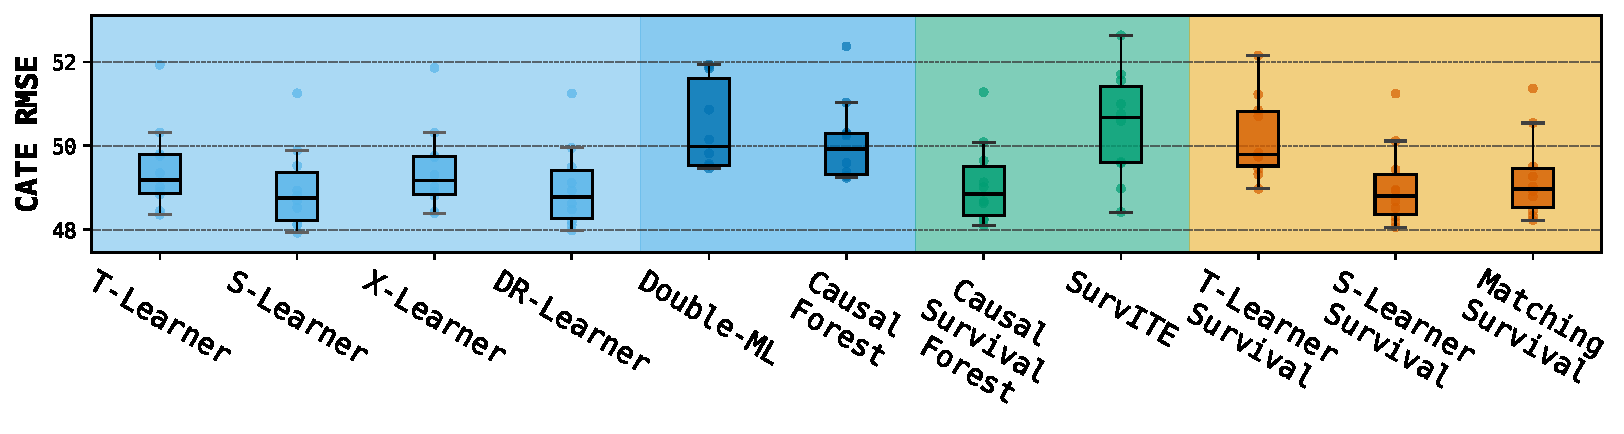
\includegraphics[width=0.7\linewidth]{Appendices/appendix-ch04/images/figure_results_updated/real_data/twin_scenario_1_twin180_cate_rmse.pdf}
   
}
\end{figure}




\subsubsection{ACTG 175 HIV clinical trial dataset} \label{ch04:subapp:hiv-data-additional-result}

We use data from the AIDS Clinical Trials Group Protocol 175 (ACTG 175) \citep{hammer1996atrial}, a double-blind, randomized controlled trial that compared four treatment regimens in adults infected with HIV type I: monotherapy with zidovudine (ZDV), monotherapy with didanosine (ddI), combination therapy with ZDV and ddI, or combination therapy with ZDV and zalcitabine (Zal).
The publicly available dataset\footnote{\url{https://archive.ics.uci.edu/dataset/890/aids+clinical+trials+group+study+175}} includes 2,139 HIV-infected patients randomized into four groups with assigned treatments: ZDV, ZDV+ddI, ZDV+Zal, and ddI.
An event occurrence was defined as the first of either a decline in CD4 cell count, an event indicating AIDS progression, or death. 

Following \citet{meir2025heterogeneous}, after fetching raw data from the UCI Machine Learning Repository, we change the resolution from days to months and add synthetic censoring based on a Bernoulli distribution with parameter $p=0.6+0.25 \cdot Z30$, where $Z30$ is a feature that is available in the data and indicates whether a patient started taking ZDV prior to the assigned treatment, and it is not included in the covariates for CATE estimation. 
We conduct three pairwise comparisons with ZDV as the baseline treatment ($W=0$): ZDV vs. ZDV+ddI (HIV1), ZDV vs. ZDV+Zal (HIV2), and ZDV vs. ddI (HIV3).
The baseline censoring rate is less than 15\% for different treatment groups.
After applying the censoring injection procedure from \citet{meir2025heterogeneous}, increasing censoring rates to over 90\%.
For each treatment group, we establish baseline CATE estimates by running Causal Survival Forests 10 times and averaging the estimated conditional average treatment effects.
Since there are many variants of outcome imputation and survival meta-learner families due to different imputation and base learner options, for display purposes in the HIV dataset results, we use a model selection criterion based on closeness (CATE RMSE) to estimation by Causal Survival Forests.
We have looked at the results using other variants of same CATE estimator as well, and similar trends are observed.

In Section~\ref{ch04:sec:real-data}, we display the comparisons of CATE estimates between baseline and high-censoring conditions for group HIV1.
Here we display the same sets of results for HIV2 and HIV3 groups in Figure~\ref{ch04:fig:hiv2-cate-estimate-comparison}, \ref{ch04:fig:hiv3-cate-estimate-comparison}.
Consistent patterns emerge across all three treatment comparisons: Causal Survival Forests produces estimates that cluster tightly around their baseline CATE estimations on data before additional censoring injection; outcome imputation methods show higher variation in baseline estimates but more concentrated predictions under high censoring, and survival meta-learners display substantial deviations from the 45-degree line, indicating sensitivity to censoring conditions.
The consistency of these patterns across different treatment pairs reinforces the robustness of our findings regarding how different estimator families respond to increased censoring.


% !TeX root = ../../../main.tex
\begin{figure}[htbp]
\ChFourFloatContents{ch04:fig:hiv2-cate-estimate-comparison}{\caption{CATE Estimation comparison between baseline and high-censoring conditions under ZDV vs. ZDV+Zal treatments (HIV2). Each point represents an individual patient in test sets, with the dashed diagonal line indicating perfect consistency between baseline CATE estimation and that with the additional censoring injected.}}{
  \centering
  
  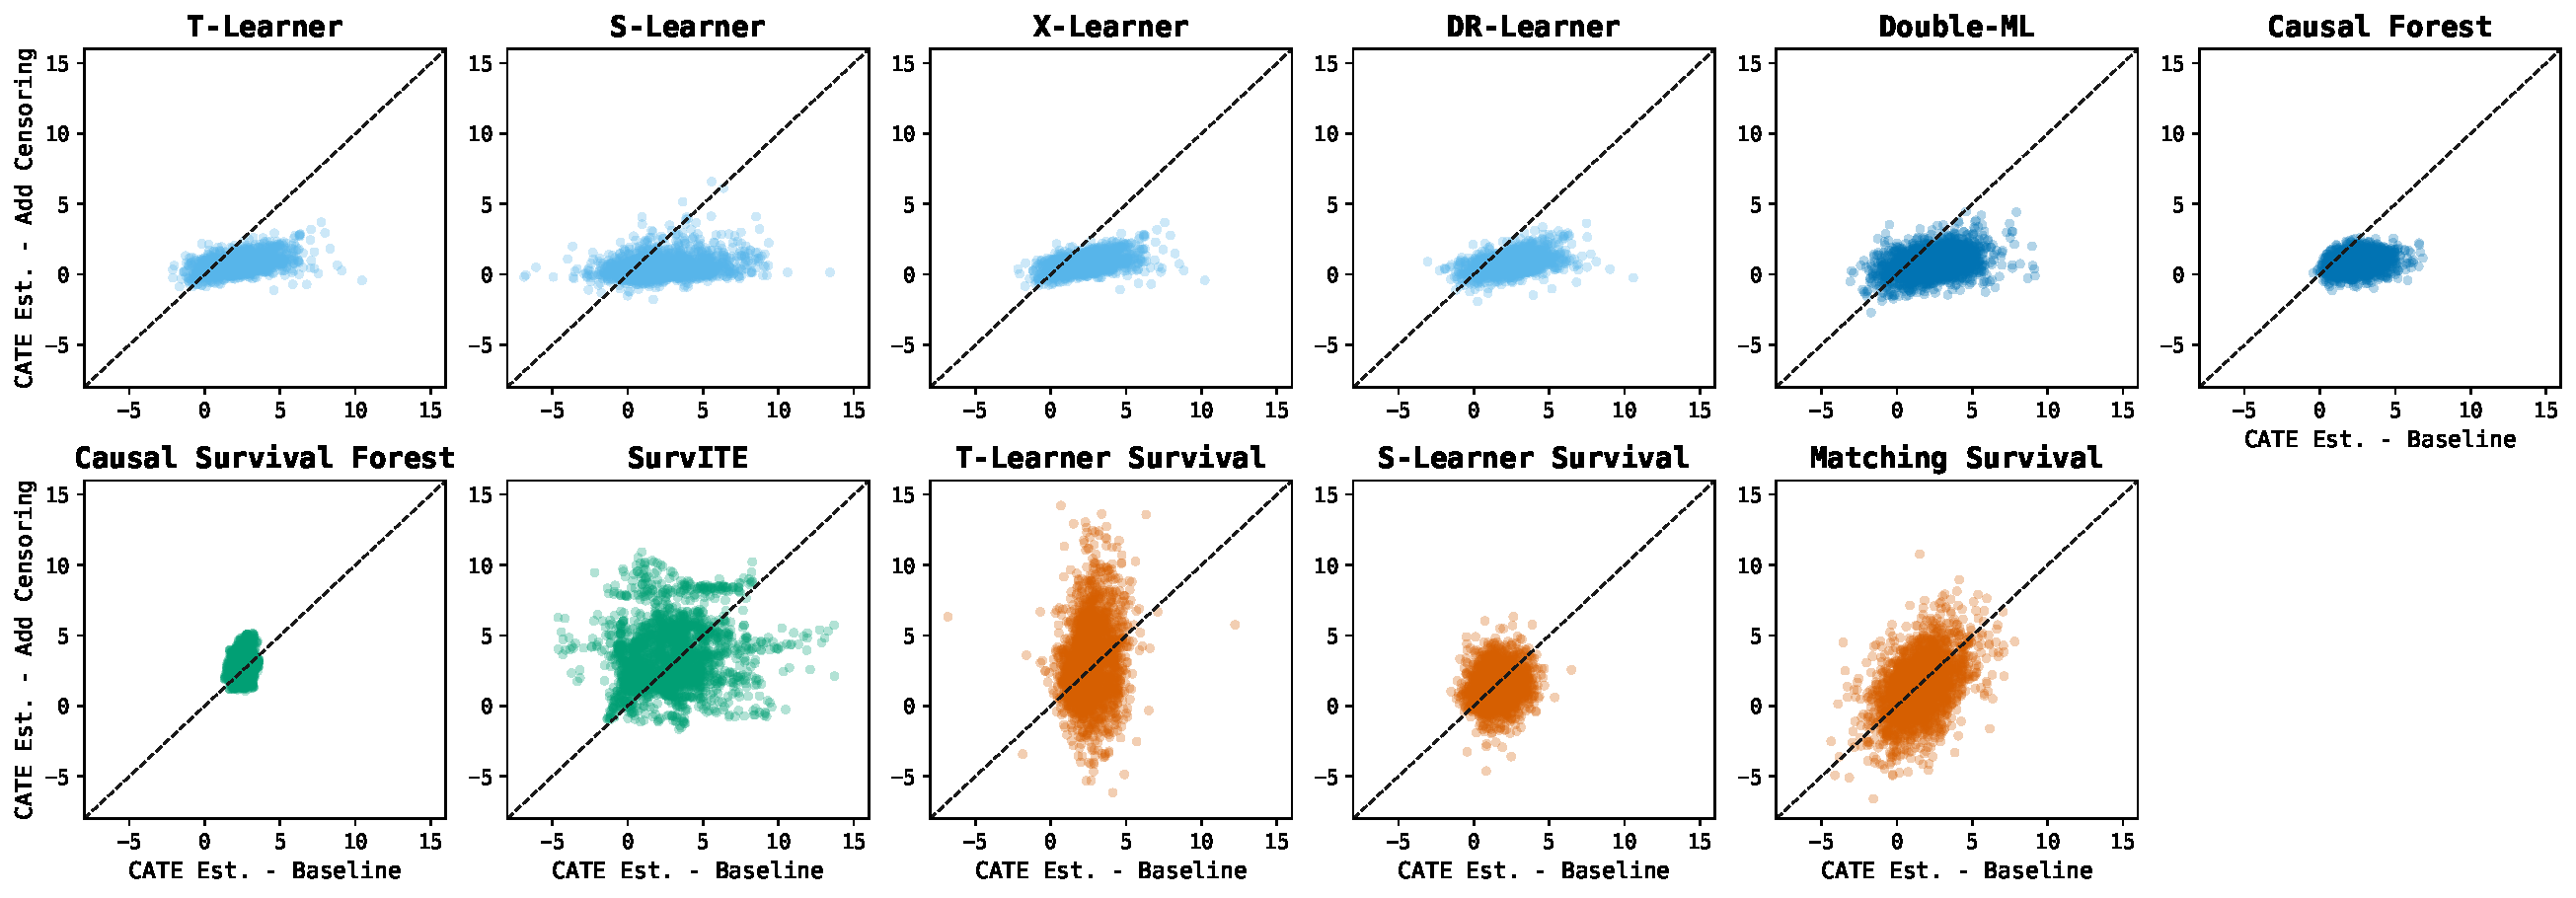
\includegraphics[width=\linewidth]{Appendices/appendix-ch04/images/figure_results_updated/real_data/ACTG_175_HIV2_CATE_comparison.pdf}
   
}
\end{figure}




% !TeX root = ../../../main.tex
\begin{figure}[htbp]
\ChFourFloatContents{ch04:fig:hiv3-cate-estimate-comparison}{\caption{CATE Estimation comparison between baseline and high-censoring conditions under ZDV vs. ddI treatments (HIV3). Each point represents an individual patient in test sets, with the dashed diagonal line indicating perfect consistency between baseline CATE estimation and that with the additional censoring injected.}}{
  \centering
  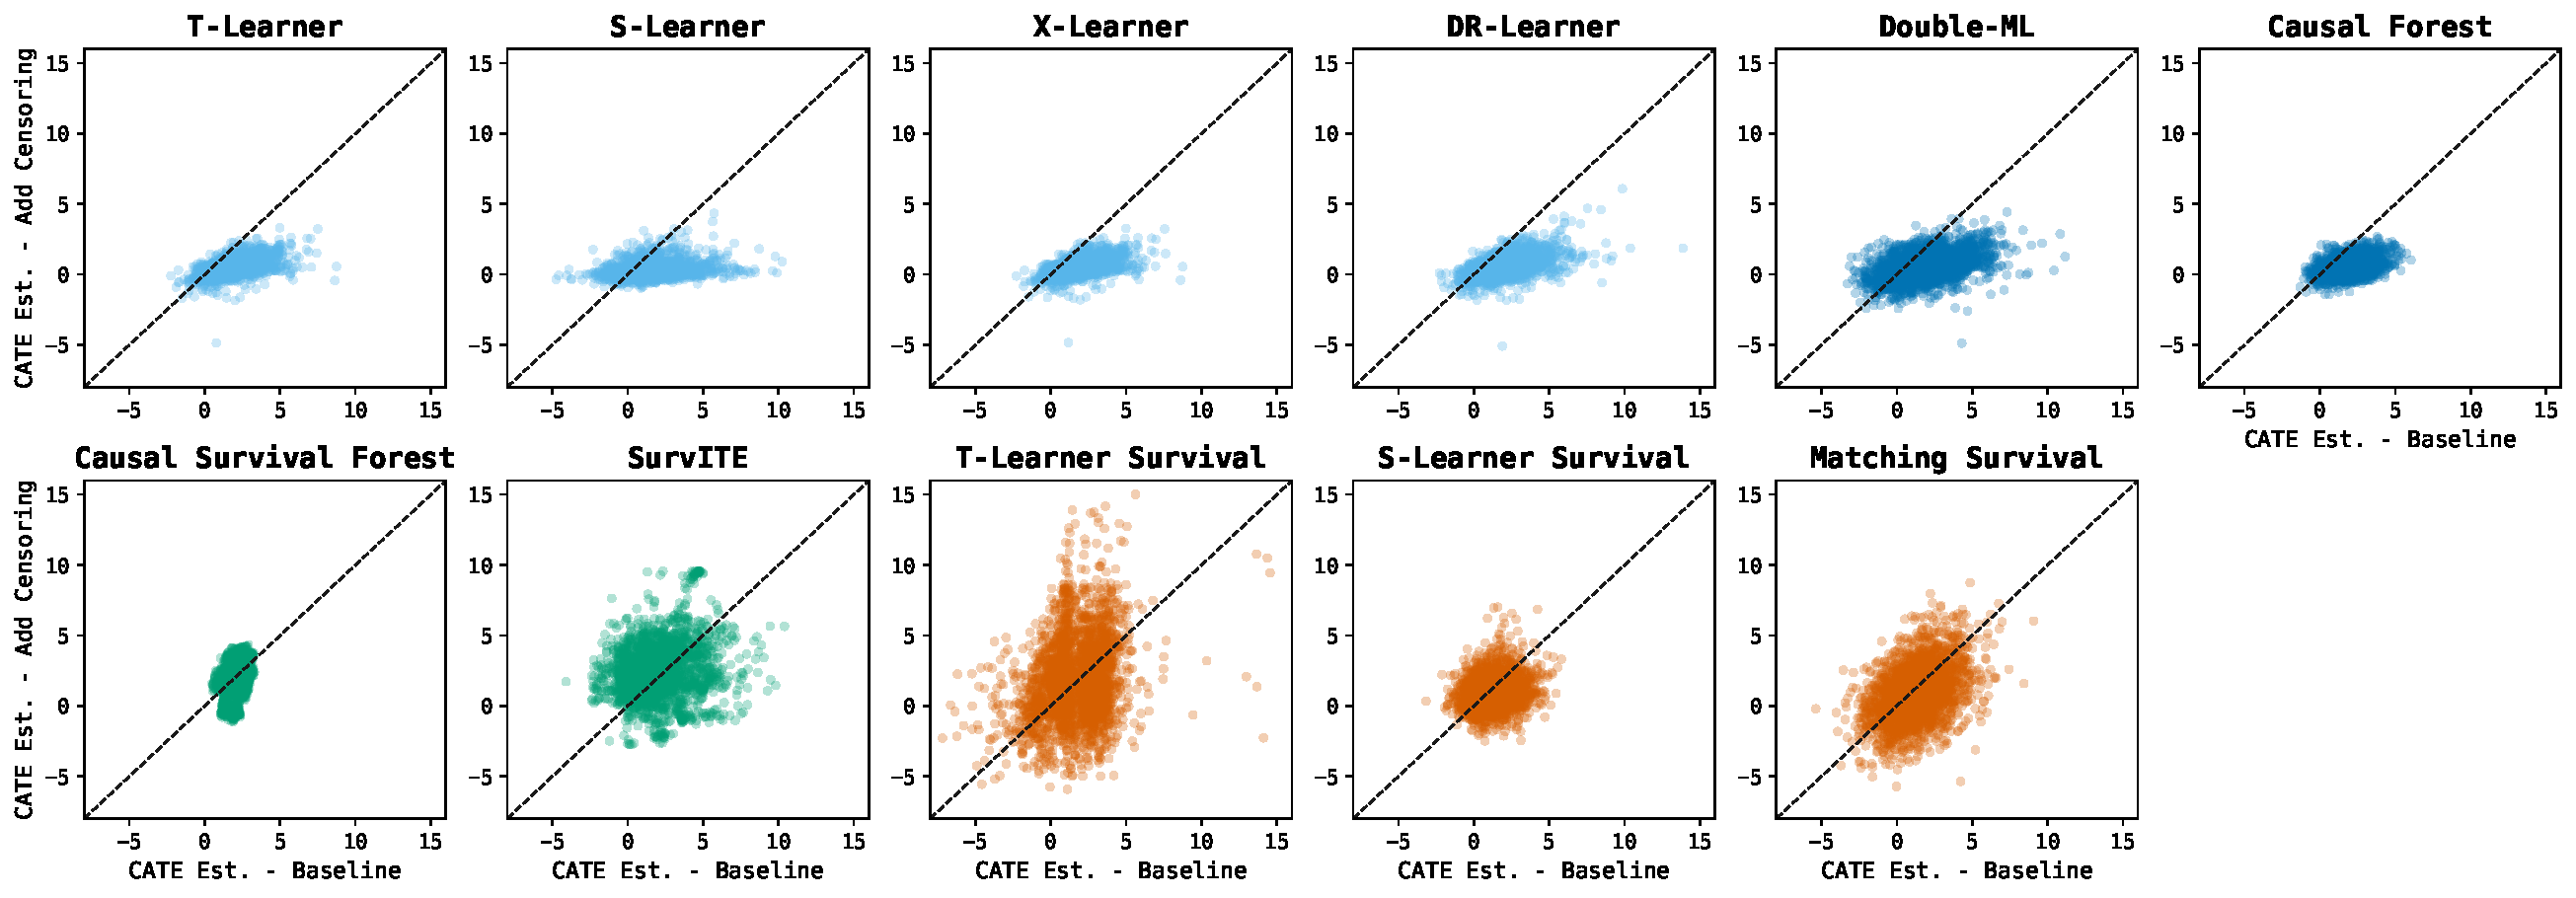
\includegraphics[width=\linewidth]
{Appendices/appendix-ch04/images/figure_results_updated/real_data/ACTG_175_HIV3_CATE_comparison.pdf}
   
}
\end{figure}







% !TeX root = ../../../main.tex
\subsection{Additional Informative Censoring via Unobserved Confounding}
\label{ch04:app:informative-censoring-uconf}
In the main paper, we model informative censoring by making censoring times stochastically dependent on event times, reflecting realistic scenarios where patients with shorter expected survival may drop out earlier. 
Here we complement this setting with an alternative mechanism where the ignorable censoring assumption is violated due to unobserved confounding. 
This extension demonstrates the flexibility of our modular data generation framework.

\ChFourParagraph{Data generation process.}
We follow the same covariate generation procedure as in our synthetic datasets: observed covariates $X \sim \text{Uniform}(0,1)^5$ and an unobserved covariate $U \sim \text{Uniform}(0,1)$. 
Treatment assignment follows the \texttt{OBS-UConf} configuration, where $U$ enters into both treatment assignment and outcome generation but remains unobserved during estimation. 

We focus on survival Scenario~\texttt{C} (Poisson hazards with medium censoring).
Event times and censoring times are generated as follows, where $w \in \{0,1\}$ is the treatment indicator:
\begin{align}
    \lambda(w) &= X_2^2 + X_3 + 6 + 2\left(\sqrt{0.3 \cdot X_1 + 0.7 \cdot U} - 0.3\right) \cdot w + \epsilon, \\
    T(w) &\sim \text{Poisson}(\lambda(w)), \\
    C &= 
    \begin{cases} 
      \infty & \text{if } U \leq 0.6, \\[0.5em]
      1 + \ChFourInd(X_{4} < 0.5) & \text{otherwise},
    \end{cases}
\end{align}
where $\epsilon \sim \mathcal{N}(0,0.1)$ adds stochastic variation. 
The censoring distribution thus depends directly on the unobserved variable $U$, creating dependence between censoring and survival that cannot be explained away by the observed $X$ alone. 

\ChFourParagraph{Summary statistics}
Similar to the other synthetic datasets, we include up to 50{,}000 samples with treatment assigned according to an observational study mechanism. 
The treatment rate is 53.9\%, the censoring rate is 39.7\% (driven by $U$), and the population-level ATE is 0.7737 (computed from the 50,000 samples by averaging the CATEs). 
This setup mirrors real-world contexts such as clinical trials with dropout patterns influenced by latent health status.

\ChFourParagraph{Experimental results}
We evaluated representative estimators from all three method families. 
Figure~\ref{ch04:fig:uconf-ic-results} reports CATE RMSE and ATE bias (mean $\pm$ standard error) across 10 random splits. 




% !TeX root = ../../../main.tex
\begin{figure}[htbp]
\ChFourFloatContents{ch04:fig:uconf-ic-results}{\caption{CATE RMSE (left) and ATE bias (right) under informative censoring induced by unobserved confounding.}}{
    \centering

\resizebox{1\textwidth}{!}{%
        \begin{minipage}{1\textwidth}

    \subfloat[{RCT:\ChFourBlackCross, Ignorability:\ChFourBlackCross, Positivity:\ChFourGrayCheck, Ignorable Censoring:\ChFourBlackCross}]{\begin{minipage}[t]{0.49\textwidth}
        \centering
        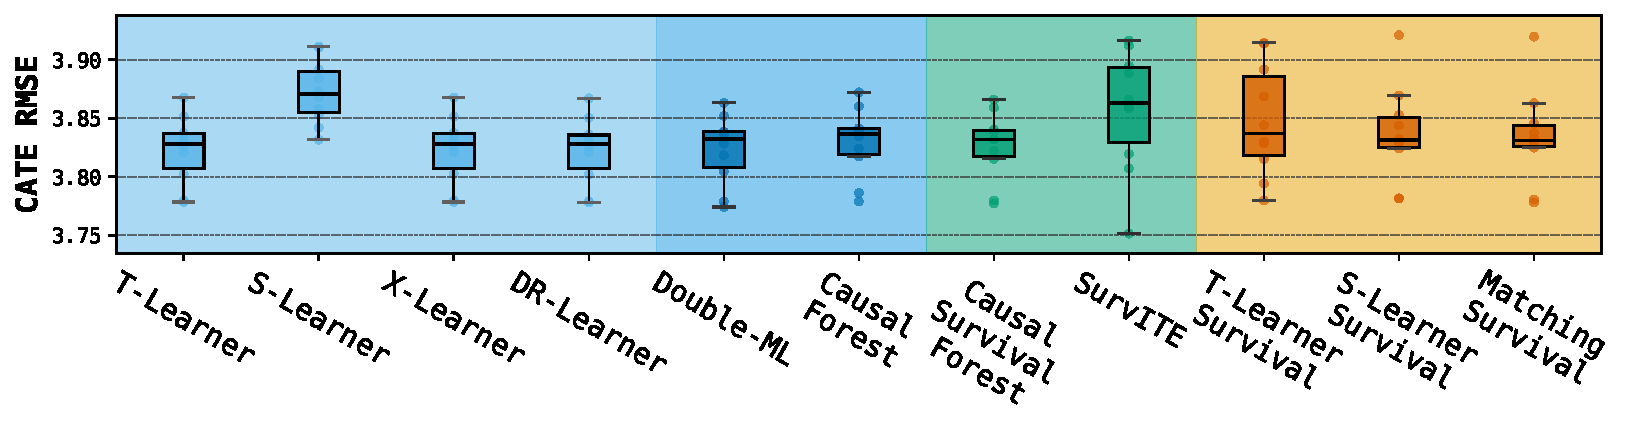
\includegraphics[width=\linewidth]{Appendices/appendix-ch04/images/figure_results_updated/unobIC_scenario_C_e_X_U_info_censor_unobserved_cate_rmse.pdf} 
       
    \end{minipage}}
    \hfill
    \subfloat[{RCT:\ChFourBlackCross, Ignorability:\ChFourBlackCross, Positivity:\ChFourGrayCheck, Ignorable Censoring:\ChFourBlackCross}]{\begin{minipage}[t]{0.49\textwidth}
        \centering
        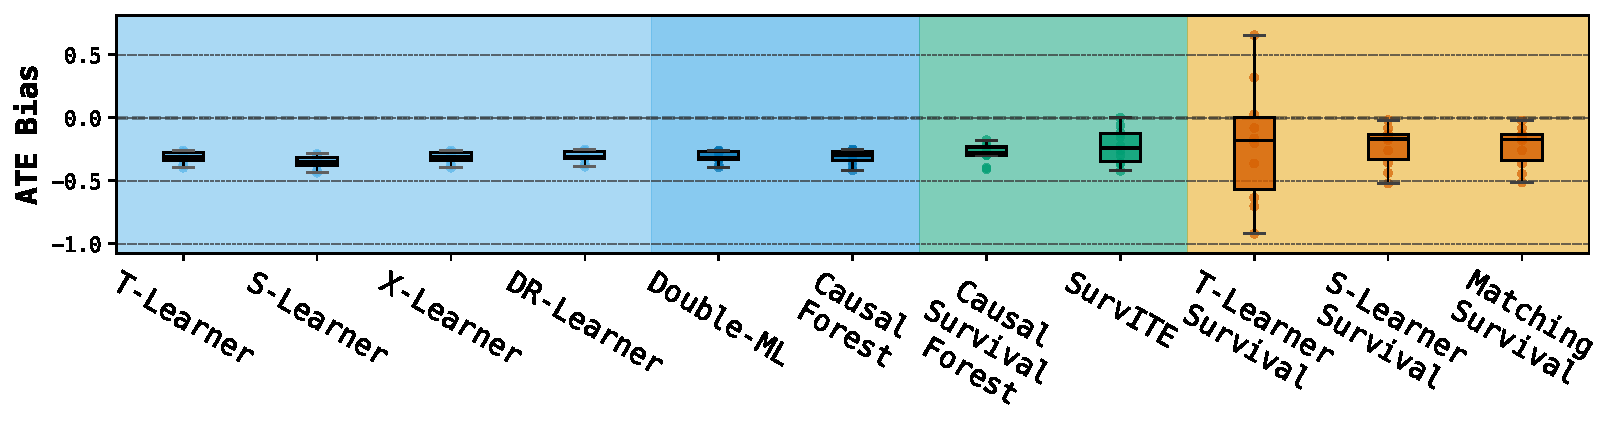
\includegraphics[width=\linewidth]{Appendices/appendix-ch04/images/figure_results_updated/unobIC_scenario_C_e_X_U_info_censor_unobserved_ate_bias.pdf} 
        
    \end{minipage}}
    \end{minipage}%
    }
    
    
    
}
\end{figure}


The results indicate that Causal Survival Forests and survival meta-learners with matching tend to perform best under this setting, consistent with findings from the main synthetic datasets. 

\ChFourParagraph{Extensibility to other settings.}
Here we illustrate one case: \texttt{OBS-UConf} combined with Scenario~\texttt{C}.  
However, the same mechanism can be straightforwardly extended to other causal configurations (e.g., randomized trials with imbalance) and survival scenarios (e.g., AFT or Cox models).  
We leave systematic exploration of these additional combinations for future work, but their ease of inclusion highlights the flexibility of \textsc{SurvHTE-Bench} to accommodate alternative censoring mechanisms.%





% CH04-SOURCE-END
\clearpage
\endgroup

% !TeX root = ../../main.tex
\begingroup
\ChFiveBegin
\emergencystretch=2em
\appendix{PMOA-TTS}\label{app:ch05}

% CH05-SOURCE-BEGIN
% !TeX root = ../../../main.tex

\begin{center}
    {\LARGE Supplementary Material: Temporally annotated longitudinal textual time series from PubMed Open Access clinical case reports}
\end{center}
 



% !TeX root = ../../../main.tex
\subsection{LLM Prompts}
\label{ch05:apd:llm-prompts}

\ChFiveHeadingOnly
\subsubsection{LLM Prompt to Generate Textual Time Series from PMOA Case Reports}
\label{ch05:apd:extraction-prompt}

% \begin{tcolorbox}[colback=gray!5, colframe=gray!100, title=LLM prompt to generate textual time series from PMOA case reports, boxrule=2pt]
\begin{tcolorbox}[
  colback=gray!5,
  colframe=gray!100,
  title=Prompt,
  boxrule=2pt,
  enhanced,
  breakable,                % <-- allows page breaks; starts here even if long
  before skip=8pt,          % spacing above (optional)
  after skip=8pt,           % spacing below (optional)
  pad at break*=2mm,        % padding at page break (optional)
  fontupper=\scriptsize,
  title after break={Prompt} % optional continuation note
]
You are a physician. Extract the clinical events and the related time stamp from the case report. The admission event has timestamp 0. If the event is not available, we treat the event, e.g. current main clinical diagnosis or treatment with timestamp 0. The events that happened before event with 0 timestamp have negative time, the ones after the event with 0 timestamp have positive time. The timestamp are in hours. The unit will be omitted when output the result. If there is no temporal information of the event, please use your knowledge and events with temporal expression before and after the events to provide an approximation. We want to predict the future events given the events happened in history. For example, here is the case report.\\

\textcolor{teal}{\texttt{An 18-year-old male was admitted to the hospital with a 3-day history of fever and rash. Four weeks ago, he was diagnosed with acne and received the treatment with minocycline, 100 mg daily, for 3 weeks. With increased WBC count, eosinophilia, and systemic involvement, this patient was diagnosed with DRESS syndrome. The fever and rash persisted through admission, and diffuse erythematous or maculopapular eruption with pruritus was present. One day later the patient was discharged.}}\\

Let's find the locations of events in the case report.
The phrase ‘a 3-day history of fever and rash’ directly places fever and rash 72 hours before admission, so both events receive timestamp \(-72\). The phrase ‘Four weeks ago’ directly places the acne diagnosis and initiation of minocycline treatment 672 hours before admission, so both events receive timestamp \(-672\). The diffuse erythematous or maculopapular eruption with pruritus is described in the admission context and is assigned timestamp 0. DRESS syndrome has no explicit timestamp, so clinical judgment is used to assign timestamp 0. The phrase ‘One day later’ places discharge 24 hours after admission.
% it shows that four weeks ago of fever and rash, four weeks ago, he was diagnosed with acne and receive treatment. So the event of fever and rash happened four weeks ago, 672 hours, it is before admitted to the hospital, so the time stamp is -672. diffuse erythematous or maculopapular eruption with pruritus was documented on the admission exam, so the timestamp is 0 hours, since it happens right at admission. DRESS syndrome has no specific time, but it should happen soon after admission to the hospital, so we use our clinical judgment to give the diagnosis of DRESS syndrome the timestamp 0. 
The output should look like:\\

%\vspace{2mm}
\texttt{18 years old | 0 \\
male | 0 \\
admitted to the hospital | 0 \\
fever | -72 \\
rash | -72 \\
acne | -672 \\
minocycline | -672 \\
increased WBC count | 0 \\
eosinophilia| 0 \\
systemic involvement| 0 \\
diffuse erythematous or maculopapular eruption| 0 \\
pruritis | 0 \\
DRESS syndrome | 0 \\
fever persisted | 0 \\
rash persisted | 0 \\
discharged | 24} \\

Separate conjunctive phrases into their component events and assign them the same timestamp (for example, separation of ‘fever and rash’ into 2 events: ‘fever’ and ‘rash’). If the event has duration, assign the event time as the start of the time interval. Attempt to use the text span without modifications except ‘history of’ where applicable. Include all patient events, even if they appear in the discussion; do not omit any events; include termination/discontinuation events; include the pertinent negative findings, like ‘no shortness of breath’ and ‘denies chest pain’. Show the events and timestamps in rows, each row has two columns: one column for the event, the other column for the timestamp. The time is a numeric value in hour unit. The two columns are separated by a pipe ‘|’ as a bar-separated file. Reply with the table only.
\end{tcolorbox}


\subsubsection{LLM Prompt to Extract Demographics from PMOA Case Reports}
\label{ch05:apd:demographics-prompt}

\ChFiveRebuttal{The prompt below is reproduced verbatim for reproducibility. Its outputs are described in the manuscript as LLM-extracted sex descriptors and LLM-mapped ethnicity categories, not as verified biological or self-identified attributes.}

\begin{tcolorbox}[
  colback=gray!5,
  colframe=gray!100,
  title={Prompt},
  boxrule=2pt,
  enhanced,
  breakable,                % <-- allows page breaks; starts here even if long
  before skip=8pt,          % spacing above (optional)
  after skip=8pt,           % spacing below (optional)
  pad at break*=2mm,        % padding at page break (optional)
  fontupper=\scriptsize,
  title after break={{Prompt}} % optional continuation note
]
You are an expert clinician. Extract the following demographic information from the case report: (1) age at case presentation, (2) sex (biologic sex at birth), and (3) ethnicity.  Report the age in years.  Report the sex as Male, Female, otherwise as a custom string, or Not Specified.  Report ethnicity as according to the US Census, otherwise as Not Specified.  For example, here is the case report.\\

\textcolor{teal}{\texttt{An 18-year-old male was admitted to the hospital with a 3-day history of fever and rash. Four weeks ago, he was diagnosed with acne and received the treatment with minocycline, 100 mg daily, for 3 weeks. With increased WBC count, eosinophilia, and systemic involvement, this patient was diagnosed with DRESS syndrome. The fever and rash persisted through admission, and diffuse erythematous or maculopapular eruption with pruritus was present. One day later the patient was discharged.}}\\

% \noindent
Then the demographic extraction should be:\\
\texttt{18 | Male | Not Specified} \\
 
Report the demographics with the three columns separated by a pipe '|' as a bar-separated row as above.
\end{tcolorbox}
% 
\subsubsection{LLM Prompt to Extract List of Diagnoses from PMOA Case Reports}
\label{ch05:apd:diagnosis-prompt}
\begin{tcolorbox}[
  colback=gray!5,
  colframe=gray!100,
  title=LLM prompt to extract list of diagnoses from PMOA case reports,
  boxrule=2pt,
  enhanced,
  breakable,                % <-- allows page breaks; starts here even if long
  before skip=8pt,          % spacing above (optional)
  after skip=8pt,           % spacing below (optional)
  pad at break*=2mm,        % padding at page break (optional)
  fontupper=\scriptsize,
  title after break={Prompt} % optional continuation note
]
\textcolor{teal}{\texttt{An 18-year-old male was admitted to the hospital with a 3-day history of fever and rash. Four weeks ago, he was diagnosed with acne and received the treatment with minocycline, 100 mg daily, for 3 weeks. With increased WBC count, eosinophilia, and systemic involvement, this patient was diagnosed with DRESS syndrome. The fever and rash persisted through admission and diffuse erythematous or maculopapular eruption with pruritus was present. One day later the patient was discharged.}} \\

Then the output should look like:\\
    \texttt{acne} \\
    \texttt{DRESS syndrome} \\

Rash, leukocytosis, and other findings are not diseases so they are omitted, while acne and DRESS syndrome were both diagnosed, so they are included. Output a list of diagnoses (one per line) from the following case. Place the primary diagnosis first. Include only the list and nothing else.

\end{tcolorbox}

\subsubsection{Timestamp Provenance Audit Prompt}
\label{ch05:apd:timestamp-provenance-prompt}
\begin{tcolorbox}[
  colback=gray!5,
  colframe=gray!100,
  title={Prompt},
  boxrule=2pt,
  enhanced,
  breakable,                % <-- allows page breaks; starts here even if long
  before skip=8pt,          % spacing above (optional)
  after skip=8pt,           % spacing below (optional)
  pad at break*=2mm,        % padding at page break (optional)
  fontupper=\scriptsize,
  title after break={{Prompt}} % optional continuation note
]
You are a physician. Extract all patient-specific clinical events and their related timestamps from the case report.


TEMPORAL ANCHOR AND TIMESTAMPS


- Assign timestamp 0 to the hospital admission event when admission is described.

- If an admission event is not available, assign timestamp 0 to the current main clinical presentation, diagnosis, or treatment used as the case reference event.

- Events before the timestamp-0 event have negative timestamps, and events after the timestamp-0 event have positive timestamps.

- Express every timestamp as a numeric value in hours and omit the unit from the output.

- If the report does not provide enough temporal information to determine an event time from the text, use surrounding events, narrative order, and clinical knowledge to provide an approximate timestamp.


KNOWN FLAG: TEXT-SUPPORTED OR RULE-DETERMINED VS \\
MODEL-IMPUTED


Add a third output column named \texttt{known}. The purpose of this flag is to distinguish timestamps that are supported by the report or fixed annotation rules from timestamps that the model has to impute or guess.

Set \texttt{known} to 1 when the assigned timestamp is supported by the source text or is fixed by the annotation rules. This includes any of the following:

- The text gives an absolute date or time, a duration, or a relative temporal expression that can be converted to hours.

- The text explicitly relates the event to the timestamp-0 event, such as ``at admission'', ``on presentation'', ``before admission'', ``after admission'', or ``hospital day 2''.

- The event itself defines the timestamp-0 anchor.

- A temporal expression in the same sentence, clause, list, paragraph, or immediately preceding sentence clearly governs the event, even when the event does not repeat the temporal phrase.

- The event is one of several findings, treatments, or outcomes described as occurring during the same explicitly timed encounter, examination, procedure, or follow-up.

- The timestamp is assigned by a fixed annotation convention rather than model judgment, such as assigning age and sex to timestamp 0.

Set \texttt{known} to 0 only when the source text does not provide enough temporal evidence for the assigned numeric timestamp and the model must supply the time using clinical judgment, an unstated assumption, narrative order alone, interpolation between other events, or another guess.

Important rules for the \texttt{known} flag:

- Do not set \texttt{known} to 0 merely because the event lacks its own temporal phrase. If the event inherits a clear time from the surrounding text, set \texttt{known} to 1.

- Converting an explicit expression such as ``three days before admission'' to -72 hours is \texttt{known = 1}.

- A vague ordering word such as ``later'' or ``subsequently'' supports event order but not a specific number of hours. If a numeric timestamp must be guessed, set \texttt{known} to 0.

- A timestamp of 0 is not automatically known. Set \texttt{known} to 1 only when timestamp 0 is supported by the text, defines the anchor, or follows a fixed annotation convention. Otherwise, set \texttt{known} to 0.

- Use \texttt{known = 0} only for genuinely model-imputed or guessed timestamps.


EXAMPLE CASE REPORT\\


\textcolor{teal}{\texttt{An 18-year-old male was admitted to the hospital with a 3-day history of fever and rash. Four weeks ago, he was diagnosed with acne and received treatment with minocycline, 100 mg daily, for 3 weeks. With increased WBC count, eosinophilia, and systemic involvement, this patient was diagnosed with DRESS syndrome. The fever and rash persisted through admission, and diffuse erythematous or maculopapular eruption with pruritus was present. One day later the patient was discharged.}} \\


EXAMPLE REASONING


The fixed annotation convention assigns age and sex to timestamp 0, so these rows have \texttt{known = 1} because their times are rule-determined rather than guessed. Admission explicitly defines timestamp 0 and has \texttt{known = 1}. The phrase ``a 3-day history of fever and rash'' directly places fever and rash 72 hours before admission, so both events have timestamp -72 and \texttt{known = 1}. The phrase ``Four weeks ago'' directly places the acne diagnosis and start of minocycline treatment 672 hours before admission, so both events have timestamp -672 and \texttt{known = 1}. Increased WBC count, eosinophilia, systemic involvement, and the DRESS syndrome diagnosis have no textual evidence that determines a specific numeric time; assigning them timestamp 0 requires clinical judgment, so they have \texttt{known = 0}. The phrase ``persisted through admission'' explicitly links persistent fever and rash to admission. The diffuse eruption and pruritus are described in the same admission-context sentence, so these events inherit timestamp 0 from that textual context. These events therefore have \texttt{known = 1}. ``One day later'' directly places discharge 24 hours after admission, so discharge has timestamp 24 and \texttt{known = 1}.


EXAMPLE OUTPUT\\


\texttt{18 years old | 0 | 1} \\
\texttt{male | 0 | 1} \\
\texttt{admitted to the hospital | 0 | 1} \\
\texttt{fever | -72 | 1} \\
\texttt{rash | -72 | 1} \\
\texttt{acne | -672 | 1} \\
\texttt{minocycline | -672 | 1} \\
\texttt{increased WBC count | 0 | 0} \\
\texttt{eosinophilia | 0 | 0} \\
\texttt{systemic involvement | 0 | 0} \\
\texttt{diffuse erythematous or maculopapular eruption | 0 | 1} \\
\texttt{pruritus | 0 | 1} \\
\texttt{DRESS syndrome | 0 | 0} \\
\texttt{fever persisted | 0 | 1} \\
\texttt{rash persisted | 0 | 1} \\
\texttt{discharged | 24 | 1} \\


EVENT EXTRACTION RULES


- Separate conjunctive phrases into their component events and assign them the same timestamp. For example, separate ``fever and rash'' into the two events ``fever'' and ``rash''.

- If an event has a duration, assign the event time as the start of the time interval.

- Use the source text span without modification whenever possible, except that ``history of'' may be added where needed to preserve meaning.

- Include all patient-specific events, even when they appear in the discussion.

- Include termination or discontinuation events and pertinent negative findings such as ``no shortness of breath'' and ``denies chest pain''.

- Do not include general medical statements, literature discussion, or events referring to people other than the index patient.


OUTPUT FORMAT


Return one event per row with exactly three pipe-separated columns in this order:\\
\texttt{event | time | known} \\

The time must be numeric and expressed in hours without a unit. The known value must be either 0 or 1. Do not use the pipe character within an event description. Return only the rows. Do not include a header, table title, explanation, Markdown, or code fences.
\end{tcolorbox}


%%%%%%%%%%%%%%%%%%%%%%%%%%%%%%%%%%%%%%%%%%%
%%%%%%%%%%%%%% Evaluation Metrics %%%%%%%%%%%
%%%%%%%%%%%%%%%%%%%%%%%%%%%%%%%%%%%%%%%%%%



% !TeX root = ../../../main.tex
\subsection{Evaluation Metrics}
\label{ch05:apd:evaluation-metrics}

We evaluated textual time series extracted from PMOA case reports along three dimensions:
(i) semantic alignment between predicted and manually annotated events (event match recall, precision, and F1),
(ii) agreement in temporal ordering (temporal concordance), and
(iii) agreement in timestamp values (time discrepancy).
Each dimension captures a distinct property of timeline quality.

\subsubsection{Event Match Rate (Recall, Precision, and F1)}
\label{ch05:apd:event-match-rate}

To assess how well predicted clinical events align with reference events, we use a recursive
best-match strategy adapted from prior work~\cite{wang2025large} as shown in Algorithm~\ref{ch05:alg:recursive_match}. At each step, the method
identifies the closest unmatched pair of predicted and reference events using a text-similarity
metric, retains the pair if it satisfies a distance threshold, and removes both events before
proceeding. \textbf{Algorithm \ref{ch05:alg:recursive_match}} provides pseudocode for this recursive matching procedure.
This strategy produces a one-to-one alignment between reference and predicted events that is
efficient and well-suited to timelines of differing lengths. 

In our final evaluation, we also implement a globally optimal one-to-one matching procedure based on the Linear Assignment Problem, solved using the Jonker–Volgenant (LAPJV) algorithm \citep{jonker1987shortest}. We construct a rectangular cost matrix of pairwise cosine distances between predicted and reference events and enforce a distance threshold by assigning infeasible pairs a prohibitively large cost. LAPJV then computes a minimum-cost assignment under these constraints, yielding a globally optimal one-to-one alignment. This provides a principled benchmark against the recursive heuristic while preserving the same matching constraints. Unlike the recursive best-match heuristic, which greedily selects local minima, the LAPJV formulation optimizes the full matching jointly, ensuring global optimality under the same one-to-one and distance constraints. A detailed sensitivity analysis of LAPJV-based matching with respect to the distance threshold,
including trade-offs between event match recall, temporal concordance, and timestamp accuracy, is presented in Appendix~\ref{ch05:apd:lapjv-matching}. 

We evaluated several similarity measures—including Levenshtein distance, BERT-based
embeddings, and PubMedBERT embeddings—and found cosine similarity using PubMedBERT
sentence embeddings to perform best. A cosine distance threshold of 0.1 is used to determine
whether a predicted event is considered a semantic match.

% Under this procedure, the event match rate is defined as:
% \[
% \text{Match Rate} =
% \frac{\#\{\text{reference events with a matched prediction}\}}
%      {\#\{\text{reference events}\}},
% \]
% which measures the proportion of reference events that are successfully recovered.

\ChFiveRebuttal{
We evaluate event identification using event match recall, precision, and F1. Let $M$ denote the number of one-to-one semantic matches after assignment and application of the cosine-distance threshold, $N_{\mathrm{manual}}$ the number of manually annotated events, and $N_{\mathrm{model}}$ the number of model-generated events. Event match recall is defined as $M/N_{\mathrm{manual}}$, event match precision as $M/N_{\mathrm{model}}$, and event match F1 as the harmonic mean of precision and recall. Precision therefore penalizes additional model-generated events that remain unmatched under the one-to-one alignment, complementing recall, which measures the proportion of manually annotated events recovered.
}

% We provide pseudocode for the best match procedure between two lists of strings (Algorithm \ref{ch05:alg:recursive_match}).  For each list, we use the text order, \emph{i.e.}, the order of the events in the annotation files, to break embedding distance ties.  We use the cosine similarity for the distance calculation using sentence transformer embeddings from \texttt{S-PubMedBert-MS-MARCO}.


% !TeX root = ../../../main.tex
\begin{ChFiveAlgorithm}[ht]
\caption{Recursive Best Match}
\scriptsize
\label{ch05:alg:recursive_match}
\begin{algorithmic}[1]
\ChFiveAlgRequire Two lists: \texttt{ref} (manually annotated reference events) and \texttt{pred} (predicted events)
\ChFiveAlgEnsure List of best-matching event pairs
\ChFiveAlgFunction{MatchEvents}{\texttt{ref}, \texttt{pred}}
    \ChFiveAlgIf{\texttt{ref} is empty \textbf{or} \texttt{pred} is empty}
        \ChFiveAlgState \ChFiveAlgReturn \texttt{[]}
    \ChFiveAlgEndIf
    \ChFiveAlgState $\texttt{min\_distance} \gets \infty$
    \ChFiveAlgState $\texttt{best\_pair} \gets \texttt{None}$
    \ChFiveAlgForAll{$r \in \texttt{ref}$}
        \ChFiveAlgForAll{$p \in \texttt{pred}$}
            \ChFiveAlgState $d \gets \texttt{ComputeDistance}(r, p)$
            \ChFiveAlgIf{$d < \texttt{min\_distance}$}
                \ChFiveAlgState $\texttt{min\_distance} \gets d$
                \ChFiveAlgState $\texttt{best\_pair} \gets (r, p)$
            \ChFiveAlgElsIf{$d = \texttt{min\_distance}$}
                \ChFiveAlgState $(r^*, p^*) \gets \texttt{best\_pair}$
                \ChFiveAlgState Get indices (within the annotation files) of $r$, $p$, and also of $r^*, p^*$
                \ChFiveAlgIf{index of $r <$ index of $r^*$}
                    \ChFiveAlgState $\texttt{best\_pair} \gets (r, p)$
                \ChFiveAlgElsIf{index of $r = $ index of $r^*$ \textbf{and} index of $p <$ index of $p^*$}
                    \ChFiveAlgState $\texttt{best\_pair} \gets (r, p)$
                \ChFiveAlgEndIf
            \ChFiveAlgEndIf
        \ChFiveAlgEndFor
    \ChFiveAlgEndFor
    \ChFiveAlgState $(r^*,p^*) \gets \texttt{best\_pair}$
    \ChFiveAlgState Remove $r^*$ from \texttt{ref}
    \ChFiveAlgState Remove $p^*$ from \texttt{pred}
    \ChFiveAlgState $\texttt{result} \gets \texttt{[best\_pair]} + \texttt{MatchEvents}(\texttt{ref}, \texttt{pred})$
    \ChFiveAlgState \ChFiveAlgReturn $\texttt{result}$
\ChFiveAlgEndFunction
\end{algorithmic}
\end{ChFiveAlgorithm}



% \begin{table}[ht!]
% \vspace{-3.5mm}
% \centering
% \caption{Bootstrap 95\% confidence intervals for Match Rate, Concordance, and AULTC across models evaluated on the 200 manually annotated case reports.
% %\jeremy{suggest being consistent about number of sigfigs in results (see table 2)}
% }
% \label{tab:bootstrap_intervals}
% \begin{tabular}{lccc}
% \hline
% \textbf{Model} & \textbf{Match Rate (95\% CI)} & \textbf{Concordance (95\% CI)} & \textbf{AULTC (95\% CI)} \\
% \hline
% \texttt{Llama 3.3 70B}      & [0.642, 0.718] & [0.833, 0.861] & [0.701, 0.754] \\
% \texttt{DeepSeek-R1}        & [0.694, 0.773] & [0.783, 0.818] & [0.708, 0.752] \\
% \texttt{DeepSeek-V3-0324}   & [0.727, 0.791] & [0.792, 0.821] & [0.718, 0.758] \\
% \texttt{OpenAI GPT5}        & [0.805, 0.866] & [0.882, 0.898] & [0.706, 0.749] \\
% \texttt{OpenAI O4-mini}     & [0.692, 0.767] & [0.826, 0.852] & [0.732, 0.769] \\
% \texttt{OpenAI O3}          & [0.699, 0.766] & [0.888, 0.907] & [0.728, 0.765] \\
% \texttt{OpenAI O1}          & [0.599, 0.677] & [0.872, 0.895] & [0.716, 0.755] \\
% \hline
% \end{tabular}
% \vspace{-3.5mm}
% \end{table}


\subsubsection{Temporal Concordance}
\label{ch05:apd:temporal-concordance}

Temporal ordering accuracy is quantified using the concordance index (c-index), which
measures agreement in the ordering of pairs of matched events.
Let $t^{\text{ref}}_i$ and $t^{\text{pred}}_i$ denote the reference and predicted timestamps for
matched event $i$.

\ChFiveRebuttal{
Comparable pairs are formed within each report from matched events with usable timestamps. Pairs with equal manual-reference timestamps are excluded from the concordance denominator. Among the remaining pairs, equal model timestamps receive 0.5 credit. We report the summed number of comparable pairs, the number and percentage of manual-reference ties among all eligible pairs, and the number and percentage of model ties among comparable pairs for each model.
}

The c-index is:
\[
\text{c-index}
=
\frac{1}{N}
\sum_{\substack{i<j\\
t^{\text{ref}}_i \neq t^{\text{ref}}_j}}
\left[
\mathds{1}\!\left\{
(t^{\text{ref}}_i-t^{\text{ref}}_j)
(t^{\text{pred}}_i-t^{\text{pred}}_j)>0
\right\}
+
\frac{1}{2}
\mathds{1}\!\left\{
t^{\text{pred}}_i=t^{\text{pred}}_j
\right\}
\right],
\]
where $N$ is the number of comparable pairs. Higher values indicate stronger preservation of reference ordering.

\ChFiveRebuttal{
In our analysis of 200 manually annotated benchmark, manual-reference ties accounted for 13.81\%--15.37\% of all eligible pairs, while LLM annotation ties occurred in 14.16\%--34.70\% of comparable pairs (Table \ref{ch05:tab:concordance_pairs_ties}). Counts were summed across documents, and percentages were calculated from the corresponding summed counts. Manual-reference tie rates differ across models because each model yields a different set of matched events with usable timestamps.
}


% !TeX root = ../../../main.tex
\begin{table}[htbp]
\caption{\ChFiveRebuttal{Comparable event pairs and timestamp ties used in the concordance analysis. Manual-reference tie percentages are calculated among all eligible pairs, whereas model tie percentages are calculated among comparable pairs.}}\ChFiveFloatLabel{ch05:tab:concordance_pairs_ties}
\ChFiveTableBodyStart
\begin{ChFiveFloatBody}

\centering
\footnotesize
\setlength{\tabcolsep}{5pt}


\begin{tabular}{lrrr}
\hline
\textbf{Model} &
\textbf{Comparable pairs} &
\begin{tabular}{c}\textbf{Manual-reference}\\\textbf{ties, n (\%)}\end{tabular} &
\begin{tabular}{c}\textbf{Model ties among}\\\textbf{comparable pairs, n (\%)}\end{tabular} \\
\hline
\texttt{Llama 3.3 70B} & 167,738 & 30,470 (15.37\%) & 42,299 (25.22\%) \\
\texttt{DeepSeek-R1}    & 200,183 & 33,937 (14.50\%) & 68,455 (34.20\%) \\
\texttt{DeepSeek-V3}    & 229,576 & 38,338 (14.31\%) & 79,667 (34.70\%) \\
\texttt{OpenAI GPT-5}   & 278,804 & 44,816 (13.85\%) & 39,475 (14.16\%) \\
\texttt{OpenAI O4-mini} & 214,768 & 34,752 (13.93\%) & 56,536 (26.32\%) \\
\texttt{OpenAI O3}      & 203,830 & 32,671 (13.81\%) & 33,255 (16.32\%) \\
\texttt{OpenAI O1}      & 150,708 & 27,190 (15.28\%) & 29,424 (19.52\%) \\
\hline
\end{tabular}

\end{ChFiveFloatBody}
\end{table}


\subsubsection{Time Discrepancy and AULTC}
\label{ch05:apd:aultc}

For each matched event, we measure timestamp accuracy using the absolute time error
$\Delta t_i = |t^{\text{pred}}_i - t^{\text{ref}}_i|$.  
Because timestamp discrepancies can vary across several orders of magnitude, we evaluate
errors on a log scale:
\[
x_i = \log(1 + \Delta t_i).
\]

To characterize timestamp accuracy across the dataset, we compute the empirical CDF (constructed over log-time discrepancies pooled across all matched events in the 200-case gold standard):
\[
F(x) = \frac{1}{k} \sum_{i=1}^{k} \mathds{1}\{x_i \le x\},
\]
where $k$ is the total number of matched events across all annotated cases.

\ChFiveRebuttal{
AULTC is computed over semantically matched event pairs only and therefore measures timestamp accuracy conditional on successful event alignment. Unmatched events do not enter the empirical CDF or AULTC and are evaluated separately by the event-extraction metrics. A single common $S_{\max}$ is used to normalize AULTC for all models and runs, avoiding model-specific rescaling.
}

We then summarize the overall discrepancy using the Area Under the Log-Time CDF (AULTC):
\[
\text{AULTC} =
\frac{1}{\log(1+S_{\max})}
\left[
\sum_{i=1}^{k}(x_{(i)} - x_{(i-1)})\frac{i}{k}
+
\big( \log(1+S_{\max}) - x_{(k)} \big)
\right],
\]
where $x_{(i)}$ are the sorted log discrepancies and $S_{\max}$ is the common maximum observed absolute error across all models and runs being compared.
AULTC ranges from 0 to 1, with higher values indicating closer alignment between predicted
and reference timestamps.

Finally, we stratify timestamp errors by temporal distance (e.g., within 1 hour, 1 day, 1 week,
1 year) to examine how accuracy varies across clinically meaningful time scales.




%%%%%%%%%%%%%%%%%%%%%%%%%%%%%%%%%%%%%%%%%
%%%%%%%%%%%%% UMLS mapping %%%%%%%%%%%%%%
%%%%%%%%%%%%%%%%%%%%%%%%%%%%%%%%%%%%%%%%


% !TeX root = ../../../main.tex
\subsection{UMLS Mapping for Diagnosis Standardization}
\label{ch05:apd:umls-mapping}

To standardize the diagnoses extracted by LLMs from the case reports, we mapped the free-text diagnoses to concepts in the Unified Medical Language System (UMLS). 
This process involved the following steps:

\begin{enumerate}
    \item \textbf{Initial Extraction}: For each case report, we prompted the LLM to extract diagnoses. 
    This yielded a list of free-text diagnoses for each case report.

    \item \textbf{Entity Linking}: We used ScispaCy's entity linker model 
    \texttt{(en\_core\_sci\_lg)} with the UMLS knowledge base to map each extracted diagnosis to corresponding UMLS Concept Unique Identifiers (CUIs). 
    \ChFiveRebuttal{Each complete extracted diagnosis string is now supplied directly to the UMLS candidate generator.}

    \item \textbf{Filtering and Disambiguation}: For each diagnosis, we:
    \begin{itemize}
        \item Retained only mappings with a confidence score above 0.85.
        \item \ChFiveRebuttal{When candidates are tied or near-tied, the selection procedure favors exact normalized canonical-name matches, recognized canonical suffixes, and concepts whose canonical name contains the complete diagnosis phrase.}
    \end{itemize}

    \item \textbf{Concept Normalization}: After mapping to CUIs, we:
    \begin{itemize}
        \item Retrieved the canonical names from UMLS Metathesaurus.
        % \item Applied semantic type filtering to ensure mapped concepts were of types relevant to diagnoses (e.g., "Disease or Syndrome", "Pathologic Function", "Mental or Behavioral Dysfunction")
        % \item Grouped synonym concepts where appropriate to reduce redundancy
    \end{itemize}
\end{enumerate}

% \input{Scientific_data/Supplementary/US_disease_prevalence}

This mapping process allowed us to standardize the diverse expressions of diagnoses extracted by LLMs into a consistent terminology system, enabling more reliable frequency analysis and co-occurrence patterns. 
% \textcolor{red}{Jeremy: Quantify the mapping success rate. Any effects of confidence score or justification for threshold? @Shariar}
Across the full PMOA-TTS corpus, LLM-extracted diagnoses yielded
$N_{\text{raw}} = 63{,}715$ unique free-text diagnosis strings.
Of these, $N_{\text{mapped}} = 41{,}216$ ($64.7\%$) were successfully mapped to at least one
UMLS CUI with a confidence score $\ge 0.85$.
When weighted by frequency of occurrence, mappings at this threshold covered
$91.7\%$ of all diagnosis mentions, indicating that commonly occurring clinical
diagnoses were more likely to receive high-confidence mappings.
Mapping coverage decreased monotonically with increasing confidence threshold.
We therefore selected a threshold of 0.85 as a conservative operating point for
downstream normalization, providing broad coverage of frequently occurring diagnoses
while maintaining a high-confidence mapping criterion.



% !TeX root = ../../../main.tex
\subsection{Sensitivity Analyses}
\label{ch05:apd:sensitivity-analyses}



\ChFiveHeadingOnly
\subsubsection{Sensitivity to Parts of the LLM Prompt Being Changed}
\label{ch05:apd:sensitivity-llm-prompt}

We slightly modified the prompt from the preceding section to check for sensitivity to specific parts of the LLM prompt being removed or modified.
This led to the following variants:
\begin{enumerate}\raggedright
    \item \textbf{No changes}: Original LLM query prompt. %
    
    \item \textbf{No role:} Remove the initial sentence \texttt{"You are a physician."}
    
    \item \textbf{Zero-shot prompting:} Remove the example case report and textual time series from the prompt. \\
    \textcolor{teal}{\texttt{An 18-year-old male was admitted to ...}}\\
    "Let's find the locations of events in the case report, it shows that ... then the output should look like:"\\
    \texttt{18 years old | 0 \\
    male | 0 \\
    ..}

    \item \textbf{No conjunction expansion:} Remove the following sentence from the prompt: \texttt{"Separate conjunctive phrases into their component events and assign them the same timestamp (for example, separation of ‘fever and rash’ into 2 events: ‘fever’ and ‘rash’)"}
    
    \item \textbf{Interval:} A query was added to the prompt for extracting the time interval (start and end time of clinical events).
The original prompt’s instructions and few-shot examples were modified accordingly. 
    
    \item \textbf{Interval + Type:} A query was added to the prompt for extracting the time interval and i2b2
    event type (Interval+Type), where event type is one of: Factual, Possible, Hypothetical, Conditional, Negated, Historical, Uncertain.
The original prompt’s instructions and few-shot examples were modified accordingly. 
\end{enumerate}


\ChFiveParagraph{Semantic similarity:}
The cumulative distributions of cosine distances between predicted and reference event phrases show clear differences across prompt variants. \emph{Interval} and \emph{Interval+Type} produce the closest matches, while \emph{Zero-shot} performs substantially worse, with a right-shifted distribution indicating lower-quality event spans. \emph{No role} and \emph{No conjunction} show modest degradation relative to the full prompt.
These results
demonstrate that including structured temporal guidance and explicit event formatting improves semantic alignment.

\ChFiveParagraph{Temporal ordering.}
The concordance index (c-index) follows a similar pattern. \emph{Interval+Type} achieves the highest median concordance, followed by \emph{Interval} and the full prompt.
Removing role
framing or conjunction splitting reduces ordering consistency, and \emph{Zero-shot} again yields the lowest performance with greater variability.
This suggests that structured instructions help the model maintain coherent temporal ordering among extracted events.

\ChFiveParagraph{Timestamp accuracy.}
Overall log-time discrepancy curves show that \emph{Interval} and \emph{Interval+Type} provide the most accurate timestamp predictions, whereas \emph{Zero-shot} exhibits the largest errors.
When stratified by temporal distance from presentation, prompt differences are minimal for
immediate events but widen substantially at longer horizons (1~day, 1~week, 1~year, and beyond).
Structured prompts with explicit temporal cues maintain accuracy across these
intervals, while unstructured prompts degrade more quickly.

When stratified by the time from presentation (e.g., within 1 hour, 1 day, 1 week), prompt differences are most pronounced for events occurring farther from the report anchor (Figure \ref{ch05:fig:prompt_ablation}, far right).
For immediate events, all prompt versions perform comparably.
However, at longer timescales (1 week to "ever"), Interval and Interval+Type maintain superior accuracy, while Zero-shot shows dramatic drops in performance.
This suggests that structured prompts are particularly critical for accurate long-range temporal reasoning.

Across semantic similarity, temporal ordering, and timestamp alignment, prompt components that provide explicit temporal structure or event-typing requirements consistently improve
performance, while removing instructional scaffolding—particularly in the Zero-shot condition—results in substantial degradation.
These findings highlight the importance of prompt
design in guiding LLMs to produce high-quality temporal annotations from clinical narratives.


\subsubsection{Inter-LLM Comparison of Temporal Annotations} 
\label{ch05:apd:inter-llm-comparison}

To illustrate qualitative differences among annotators, we compare temporal event sequences generated by several LLMs for a representative case report (PMC10629858) \citep{abu2023rare}, which describes a patient with lepromatous leprosy who later developed abdominal complications, recurrent bacteremia, severe sepsis, and ultimately died (Figure~\ref{ch05:fig:compare_llm_annotations}).


% !TeX root = ../../../main.tex
\begin{ChFiveUncaptionedFigure}
\begin{ChFiveFloatBody}
  \centering
    \begin{tcolorbox}[colback=white,colframe=black!30,boxrule=0.6pt,left=2mm,right=2mm,top=2mm,bottom=2mm,width=\linewidth]
    \footnotesize \textbf{Excerpt from \cite{abu2023rare}:}
    \begin{quote}\footnotesize
    A 57-year-old man recently diagnosed with lepromatous leprosy was confirmed with skin biopsy and had been on treatment (rifampicin/clofazimine/dapsone) for 2 months before admission; he was presented to the hospital with complaints of abdominal distension, constipation, vomiting, and a 10-kg weight loss. On examination, the patient was vitally stable. He had evidence of peripheral lymphadenopathy with a distended abdomen and a positive shifting dullness. A computed tomography scan of his abdomen showed mural thickening of the terminal ileum with significantly enlarged mesenteric lymph nodes, mesenteric fat stranding, and intra-abdominal free fluid, suggesting abdominal granulomatous infection or neoplastic process.
    \dots 
    
    The patient was planned for consolidation by autologous bone marrow transplant. Unfortunately, with the recurrent bacteremia and sepsis that accompanied the patient’s course due to his immunocompromised state, he was re-admitted to the medical ICU for severe sepsis and multiorgan failure and passed away around 6 months after his initial diagnosis with NHL, despite maintaining a remission status.
    \end{quote}
    \end{tcolorbox}
  \begin{minipage}[t]{0.45\linewidth}\centering
    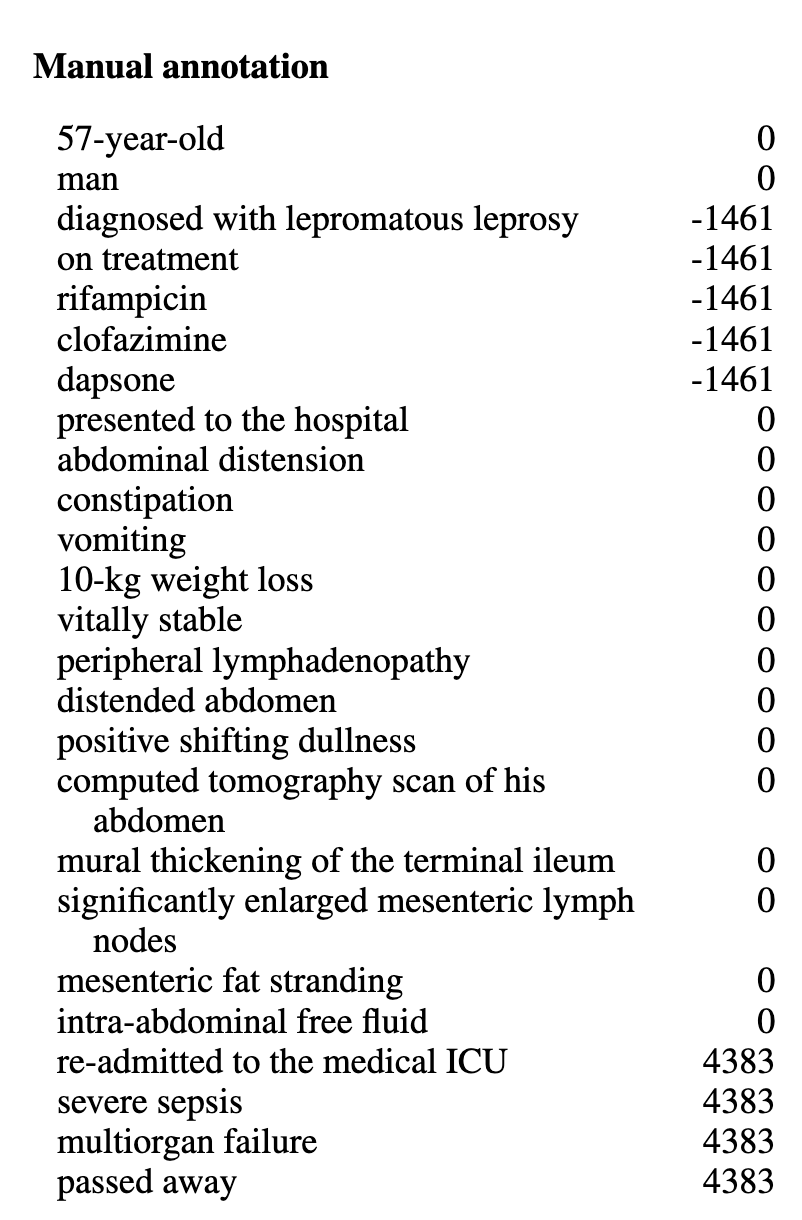
\includegraphics[width=0.9\linewidth]{Appendices/appendix-ch05/images/Scientific_data/Supplementary/example_TTS_for_paper/manual.png}
  \end{minipage}\hfill
  \begin{minipage}[t]{0.45\linewidth}\centering
    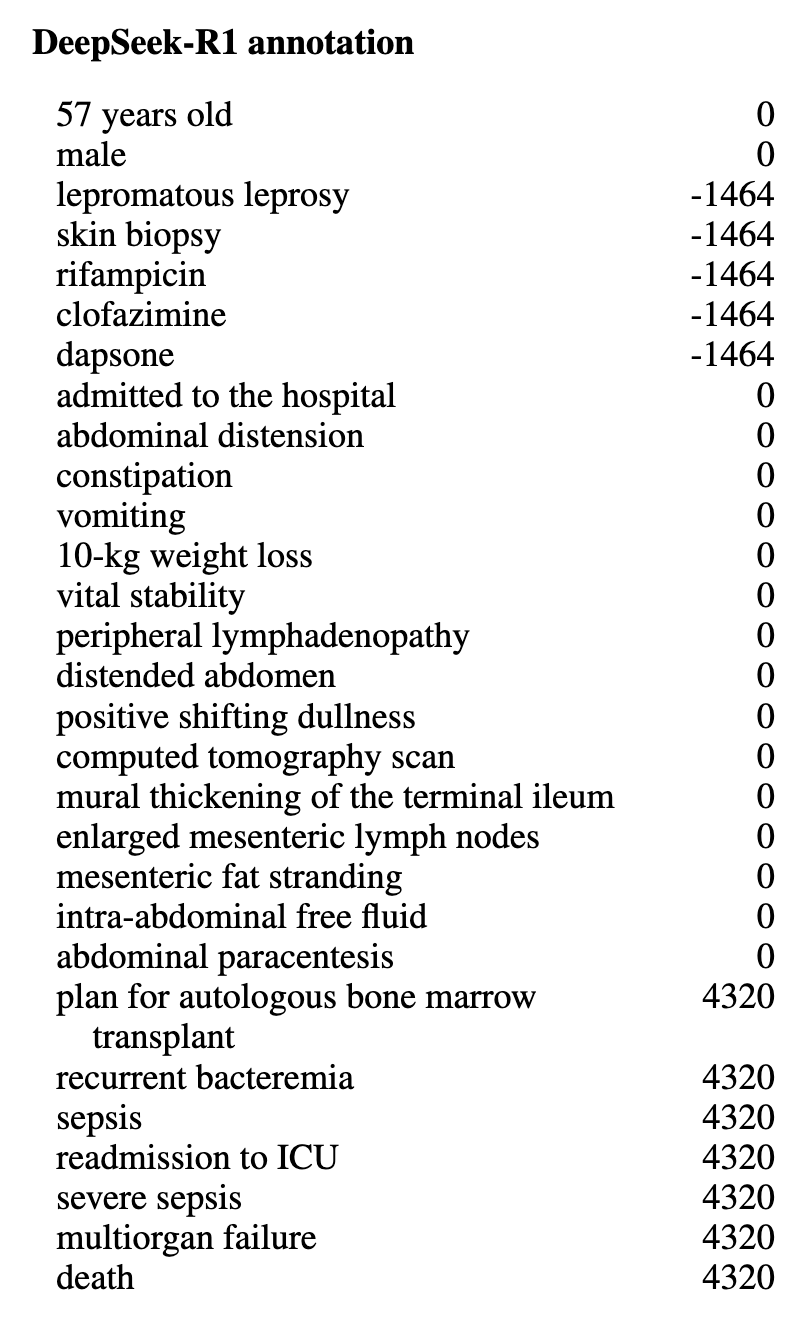
\includegraphics[width=0.9\linewidth]{Appendices/appendix-ch05/images/Scientific_data/Supplementary/example_TTS_for_paper/DeepSeekR1.png}
  \end{minipage}


  \begin{minipage}[t]{0.45\linewidth}\centering
    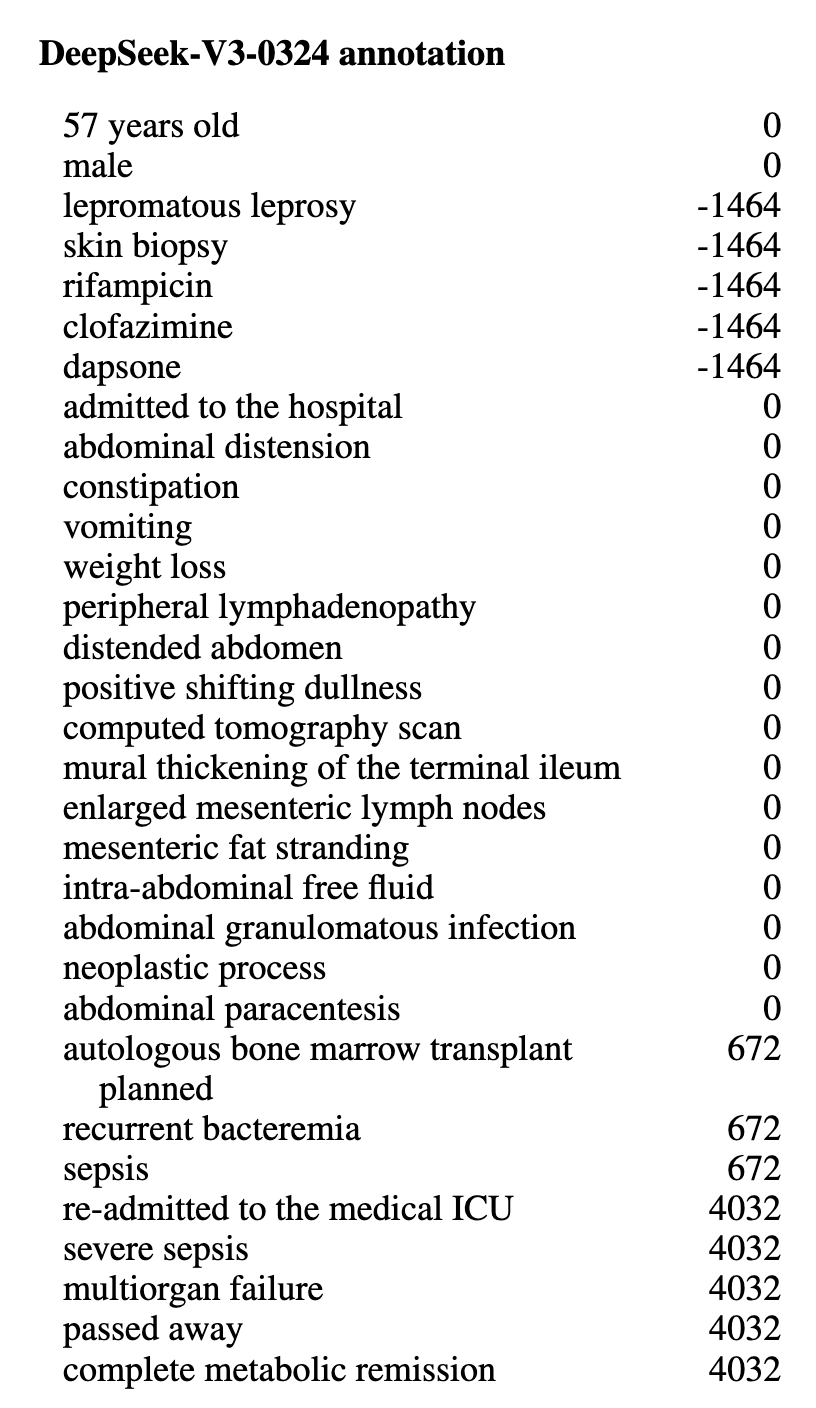
\includegraphics[width=0.9\linewidth]{Appendices/appendix-ch05/images/Scientific_data/Supplementary/example_TTS_for_paper/DeepSeekV3.png}
  \end{minipage}\hfill
  \begin{minipage}[t]{0.45\linewidth}\centering
    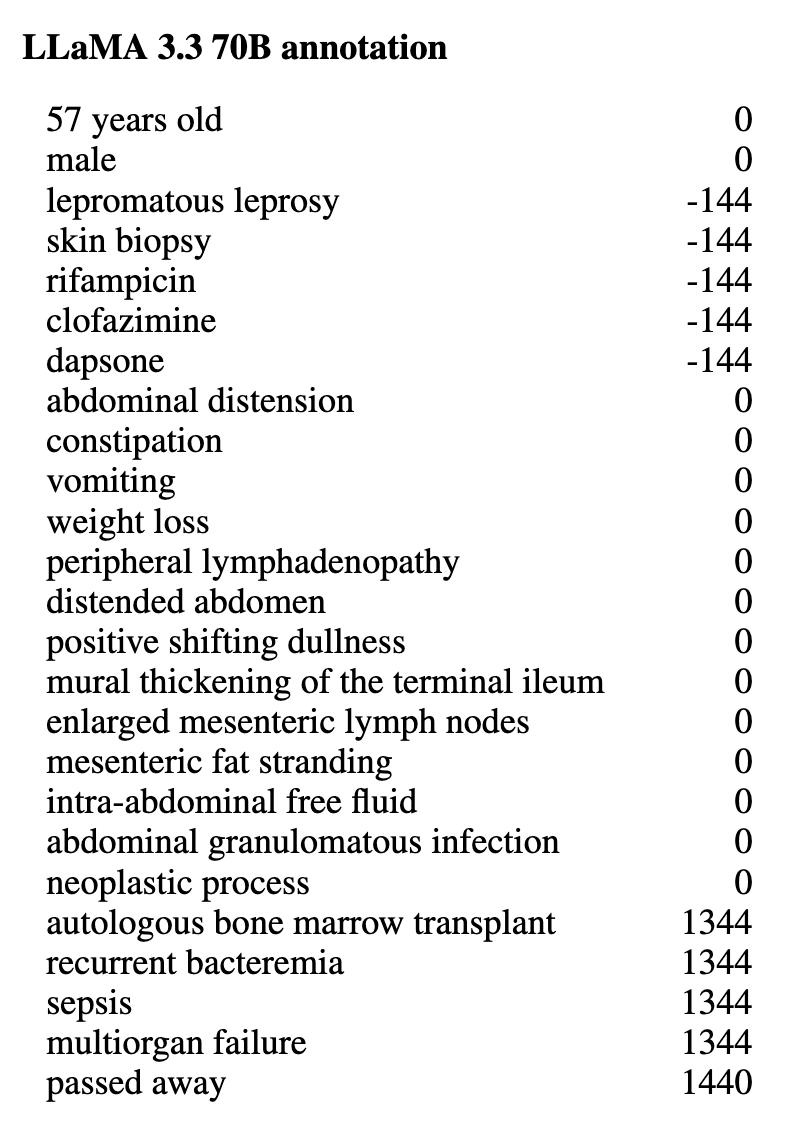
\includegraphics[width=0.9\linewidth]{Appendices/appendix-ch05/images/Scientific_data/Supplementary/example_TTS_for_paper/L3370B.png}
  \end{minipage}

\end{ChFiveFloatBody}
\end{ChFiveUncaptionedFigure}




% !TeX root = ../../../main.tex
\begin{figure}[htbp]
\begin{ChFiveFloatBody}

  \centering
  \begin{minipage}[t]{0.45\linewidth}\centering
    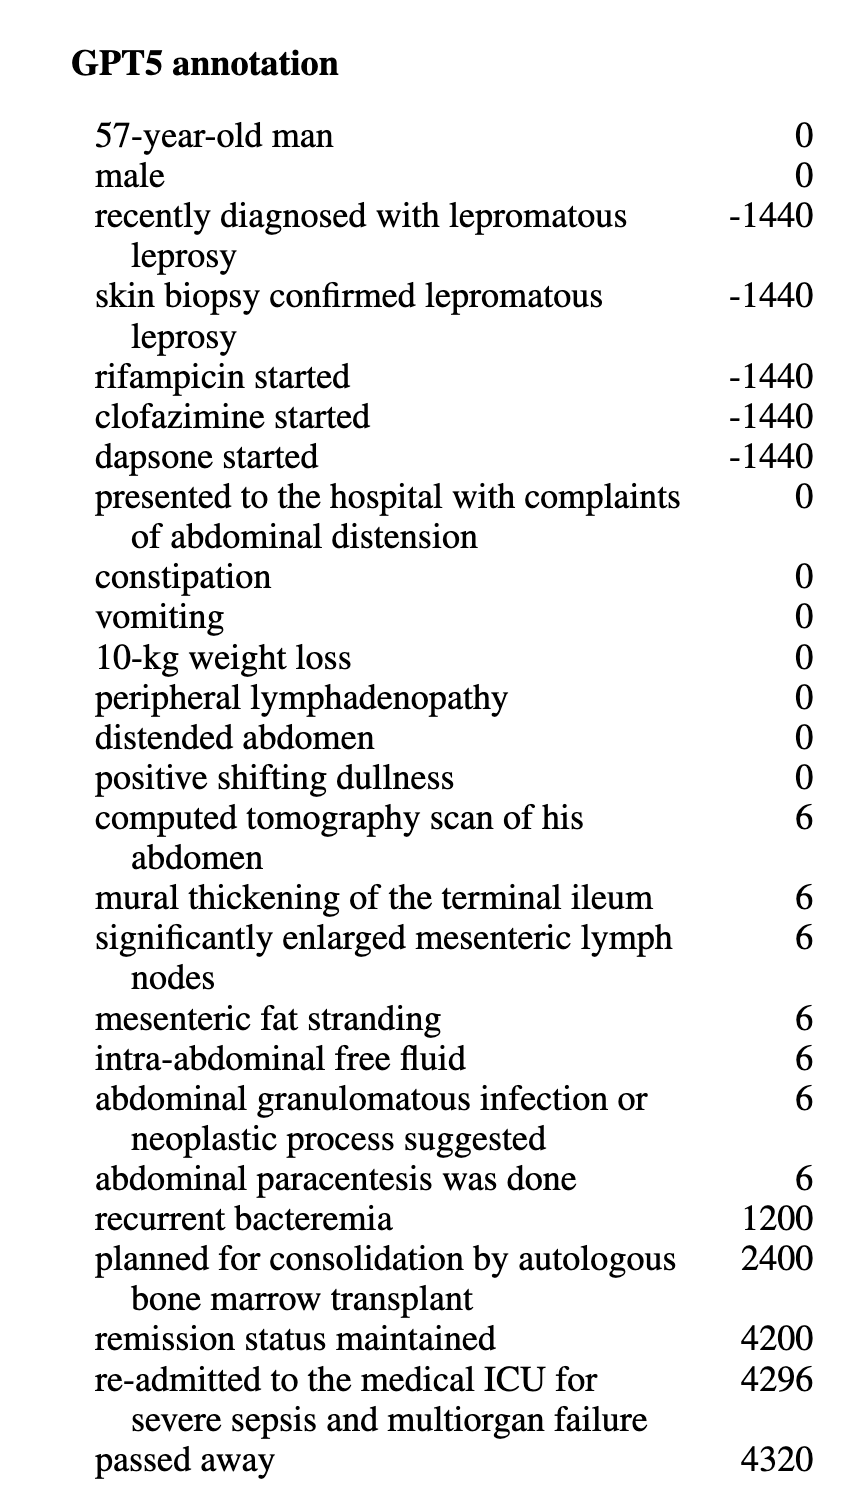
\includegraphics[width=0.9\linewidth]{Appendices/appendix-ch05/images/Scientific_data/Supplementary/example_TTS_for_paper/GPT5.png}
  \end{minipage}\hfill
  \begin{minipage}[t]{0.45\linewidth}\centering
    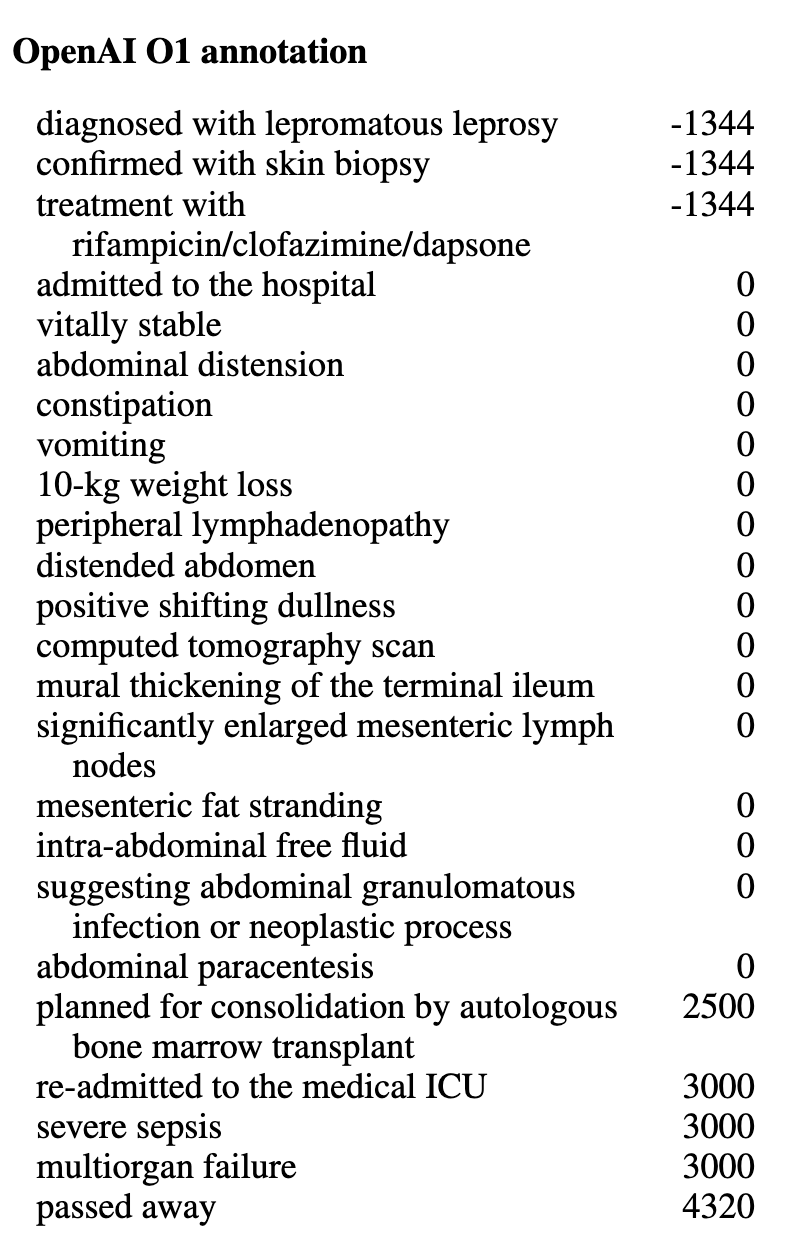
\includegraphics[width=0.9\linewidth]{Appendices/appendix-ch05/images/Scientific_data/Supplementary/example_TTS_for_paper/O1.png}
  \end{minipage}

  

  \begin{minipage}[t]{0.45\linewidth}\centering
    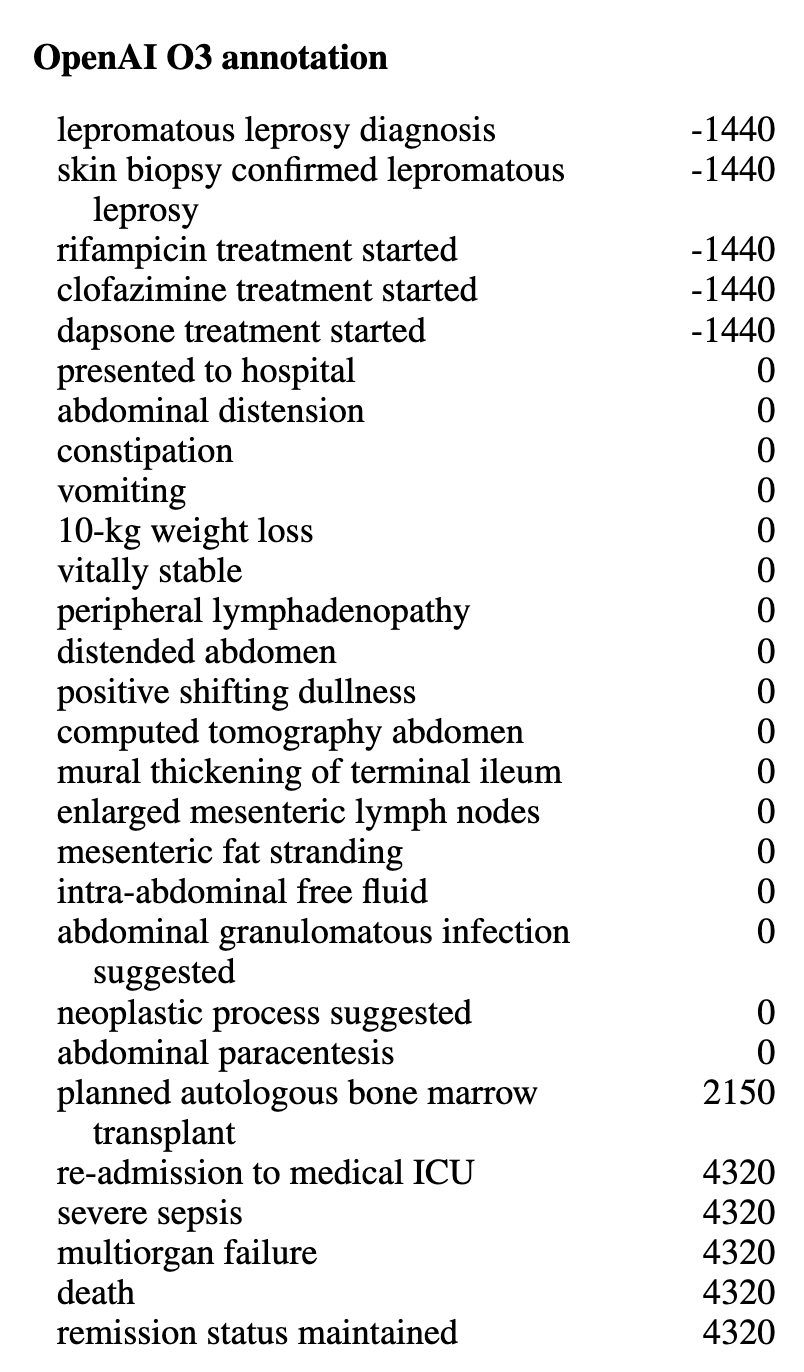
\includegraphics[width=0.9\linewidth]{Appendices/appendix-ch05/images/Scientific_data/Supplementary/example_TTS_for_paper/O3.png}
  \end{minipage}\hfill
  \begin{minipage}[t]{0.45\linewidth}\centering
    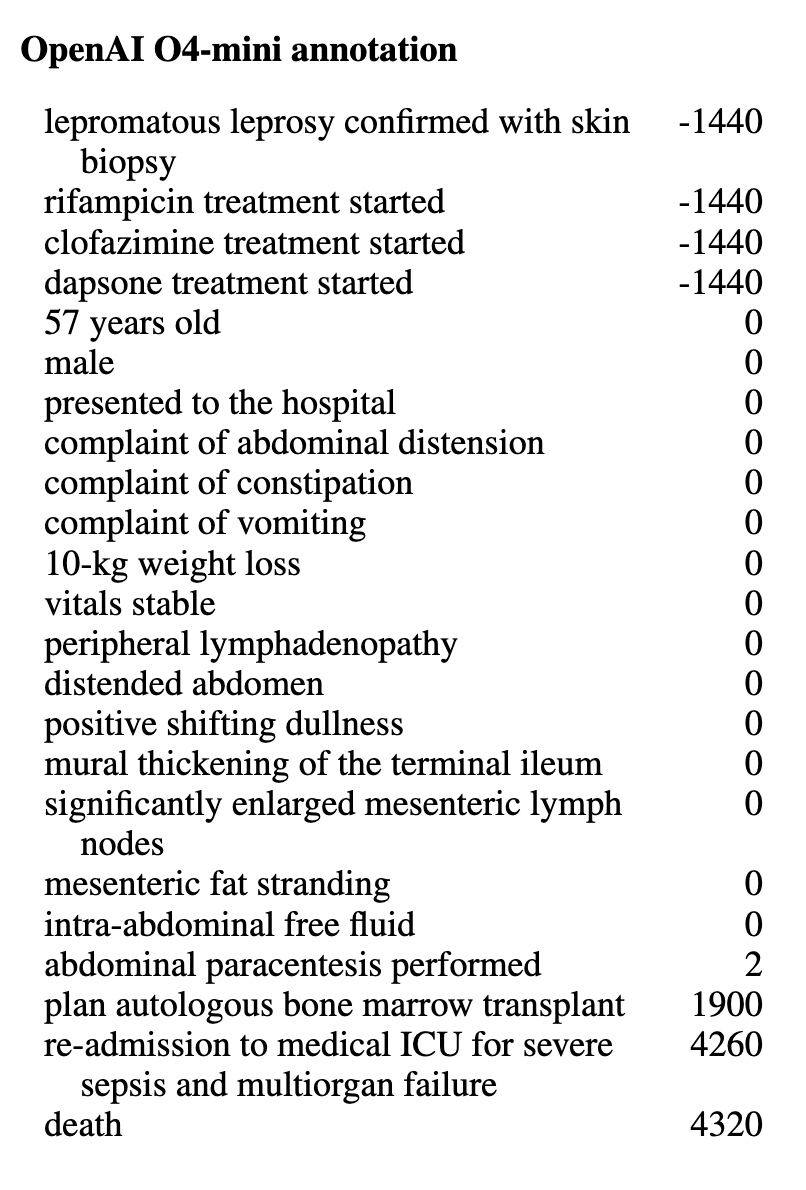
\includegraphics[width=0.9\linewidth]{Appendices/appendix-ch05/images/Scientific_data/Supplementary/example_TTS_for_paper/O4mini.png}
  \end{minipage}


  
  

\end{ChFiveFloatBody}
\caption{Comparison of temporal annotations generated by several LLMs for a representative case report (PMC10629858). The figure contrasts manual annotations with model-generated event–time
sequences, highlighting differences in event granularity, phrasing, duplicate event generation, and temporal normalization (e.g., variation in converting narrative expressions such as ``two
months before admission’’ into hour offsets). Long-range timestamp assignments (e.g., for transplant planning, ICU readmission, and death) show the greatest variability across models, whereas the overall ordering of major clinical events is largely preserved. This example illustrates characteristic
differences in how LLMs interpret, segment, and temporally anchor clinical narratives.}\ChFiveFloatLabel{ch05:fig:compare_llm_annotations}
\end{figure}



















Across models, the principal clinical trajectory is consistently recovered: confirmation of lepromatous leprosy, antibiotic treatment, evolving abdominal symptoms with corresponding imaging findings, subsequent sepsis, ICU readmission, and death.
All annotators preserve the
temporal polarity of events, assigning negative times to historical information and positive times to post-admission findings.

Differences emerge in event granularity and phrasing.
Some models split conjunctive phrases into multiple events (e.g., listing each component medication separately), whereas others
compress them into single entries.
Several annotators also produce near-duplicate events at the same timestamp (e.g., both “diagnosed with lepromatous leprosy’’ and “skin biopsy confirmed’’), reflecting variation in how models segment clinically related information within the narrative.

More pronounced differences appear in temporal normalization.
For the expression “two months before admission,” models produce hour offsets ranging from approximately $-1464$ to $-1344$, and one model assigns $-144$ due to an apparent day–hour unit error.
Long-range events such as the autologous bone marrow transplant plan, ICU readmission, and death also receive timestamps that vary by hundreds of hours across annotators.
Despite this variability in absolute timing,
the relative ordering of major clinical milestones remains largely preserved.

A recurring issue across models involves distinguishing planned actions from events that actually occurred.
For example, most annotators correctly represent “planned autologous bone-marrow transplant’’ with an associated future timestamp, which is appropriate because planned interventions can be temporally located and may influence subsequent decision-making.
However, several models omit the word “planned,’’ converting the entry into “autologous
bone-marrow transplant’’ and thereby representing an intended but unperformed procedure as an event that occurred.
In such cases, the discrepancy arises from the event label rather than the timestamp itself, illustrating how small linguistic omissions can alter the extracted temporal semantics.

% !TeX root = ../../../main.tex
\begin{table}[htbp]
\caption{Common error types observed across LLM-generated temporal annotations.}\ChFiveFloatLabel{ch05:tab:error_taxonomy}
\ChFiveTableBodyStart
\begin{ChFiveFloatBody}

\centering


\begin{tabular}{>{\raggedright\arraybackslash}p{3.2cm} >{\raggedright\arraybackslash}p{9cm}}
\toprule
\textbf{Error Type} & \textbf{Description and Examples} \\
\midrule

\textbf{Event granularity mismatch} 
& Models differ in splitting vs.\ compressing multi-component statements. 
For example, medications may appear as three separate events (``rifampicin'', ``clofazimine'', ``dapsone'') or as one combined entry. \\[6pt]

\textbf{Near-duplicate events} 
& Multiple paraphrased versions of the same clinical concept assigned to the same timestamp, such as 
``diagnosed with lepromatous leprosy’’ and 
``skin biopsy confirmed lepromatous leprosy.’’ \\[6pt]

\textbf{Temporal normalization variability} 
& Large differences in converting narrative expressions (e.g., ``two months before admission’’) to numerical timestamps, with offsets ranging from $-1464$ to $-1344$ hours and occasional scaling errors (e.g., $-144$ hours). Long-range events (e.g., transplant plan, ICU readmission, death) also vary by hundreds of hours across models. \\[6pt]

\textbf{Intent vs.\ occurrence confusion} 
& Some models omit modality markers such as ``planned,'' converting intended future events into events marked as completed. 
The timestamp itself may be reasonable; the error lies in the event label. \\[6pt]

\textbf{Phrasing and specificity variation} 
& Models differ in the level of detail used in event descriptions.  
Some outputs retain clinically precise phrases (e.g., ``mural thickening of the terminal ileum’’), while others produce generic events (e.g., ``abdominal abnormality’’). \\[6pt]

\textbf{Long-range timestamp degradation} 
& Accuracy decreases for events far from the admission anchor, with larger dispersion in timestamp predictions for events weeks or months after presentation. \\
\bottomrule
\end{tabular}


\end{ChFiveFloatBody}
\end{table}


Overall, the models capture the broad sequence of events but differ in how they segment conjunctive statements, handle near-duplicates, and resolve absolute times—particularly for
long-range events.
A taxonomy of common annotation errors observed across models—including granularity differences, duplicate events, temporal normalization variability, and intent–occurrence misclassification—is summarized in Table~\ref{ch05:tab:error_taxonomy}.


\subsubsection{Sensitivity to Event Matching Strategy (LAPJV)}
\label{ch05:apd:lapjv-matching}
We additionally consider a globally optimal one-to-one event alignment based on the Linear Assignment Problem, solved using the Jonker--Volgenant (LAPJV) algorithm \citep{jonker1987shortest}.
We define a rectangular cost matrix whose entries are pairwise cosine distances between predicted and reference events.
To enforce the same distance thresholding used in the recursive heuristic, we assign a large penalty cost to pairs whose distance exceeds the threshold, effectively masking infeasible matches.
LAPJV then computes a minimum-cost assignment under these constraints, yielding a globally optimal one-to-one alignment between the two event sets.

To assess sensitivity to the event alignment procedure, we repeat the inter-LLM comparison using LAPJV-based matching at a cosine distance threshold of 0.1.
Table~\ref{ch05:tab:model_comparison_lapjv} reports event match rate, temporal concordance, and AULTC across five independent runs per model, and is directly comparable to the main-text results obtained using the recursive matching heuristic (Algorithm~\ref{ch05:alg:recursive_match}; Table~\ref{ch05:tab:model_comparison}).
\texttt{OpenAI GPT5} achieves the highest mean match rate (0.850 $\pm$ 0.006), indicating the most comprehensive coverage of manually annotated events. \texttt{OpenAI O3} attains the highest concordance (0.894 $\pm$ 0.004), and \texttt{OpenAI O4-mini} yields the highest AULTC (0.749 $\pm$ 0.003), reflecting strong timestamp alignment among matched events. Standard deviations are generally small across runs, suggesting stable behavior for a given model.







% !TeX root = ../../../main.tex
\begin{table}[htbp]
\caption{\ChFiveRebuttal{Inter-LLM comparison under LAPJV-based event matching (threshold = 0.1), evaluated on 200 manually annotated case reports across five runs per model.}}\ChFiveFloatLabel{ch05:tab:model_comparison_lapjv}
\ChFiveTableBodyStart
\begin{ChFiveFloatBody}


\footnotesize
\centering
\setlength{\tabcolsep}{3pt}


\begin{tabular}{lccccc}
\hline
\textbf{Model} &
\begin{tabular}{c}\textbf{Event Match}\\\textbf{Recall}\end{tabular} &
\begin{tabular}{c}\textbf{Event Match}\\\textbf{Precision}\end{tabular} &
\begin{tabular}{c}\textbf{Event Match}\\\textbf{F1}\end{tabular} &
\textbf{Concordance} &
\textbf{AULTC} \\
\hline
\texttt{Llama 3.3 70B}
& 0.676 $\pm$ 0.003
& 0.761 $\pm$ 0.036
& 0.715 $\pm$ 0.015
& 0.848 $\pm$ 0.003
& 0.720 $\pm$ 0.001 \\

\texttt{DeepSeek-R1}
& 0.750 $\pm$ 0.008
& 0.793 $\pm$ 0.006
& 0.771 $\pm$ 0.006
& 0.773 $\pm$ 0.007
& 0.727 $\pm$ 0.004 \\

\texttt{DeepSeek-V3}
& 0.764 $\pm$ 0.005
& 0.801 $\pm$ 0.005
& 0.782 $\pm$ 0.004
& 0.777 $\pm$ 0.009
& 0.730 $\pm$ 0.002 \\

\texttt{OpenAI GPT-5}
& \textbf{0.851 $\pm$ 0.006}
& 0.761 $\pm$ 0.007
& \textbf{0.803 $\pm$ 0.003}
& \textbf{0.903 $\pm$ 0.004}
& 0.722 $\pm$ 0.001 \\

\texttt{OpenAI O4-mini}
& 0.752 $\pm$ 0.019
& 0.818 $\pm$ 0.015
& 0.783 $\pm$ 0.017
& 0.845 $\pm$ 0.006
& \textbf{0.750 $\pm$ 0.002} \\

\texttt{OpenAI O3}
& 0.738 $\pm$ 0.003
& 0.842 $\pm$ 0.002
& 0.786 $\pm$ 0.002
& 0.900 $\pm$ 0.005
& 0.737 $\pm$ 0.003 \\

\texttt{OpenAI O1}
& 0.640 $\pm$ 0.007
& \textbf{0.878 $\pm$ 0.003}
& 0.740 $\pm$ 0.005
& 0.881 $\pm$ 0.003
& 0.731 $\pm$ 0.002 \\
\hline
\end{tabular}


\end{ChFiveFloatBody}
\end{table}



We further examine the trade-off between event match rate and temporal accuracy by sweeping
the LAPJV distance threshold from 0.01 to 0.50 in increments of 0.01. 
Figure~\ref{ch05:fig:threshold_tradeoff_LAPJV}
plots temporal concordance and AULTC as a function of event match rate, with the operating
point at threshold 0.1 highlighted.


% !TeX root = ../../../main.tex
\begin{figure}[htbp]
\begin{ChFiveFloatBody}

    \centering
    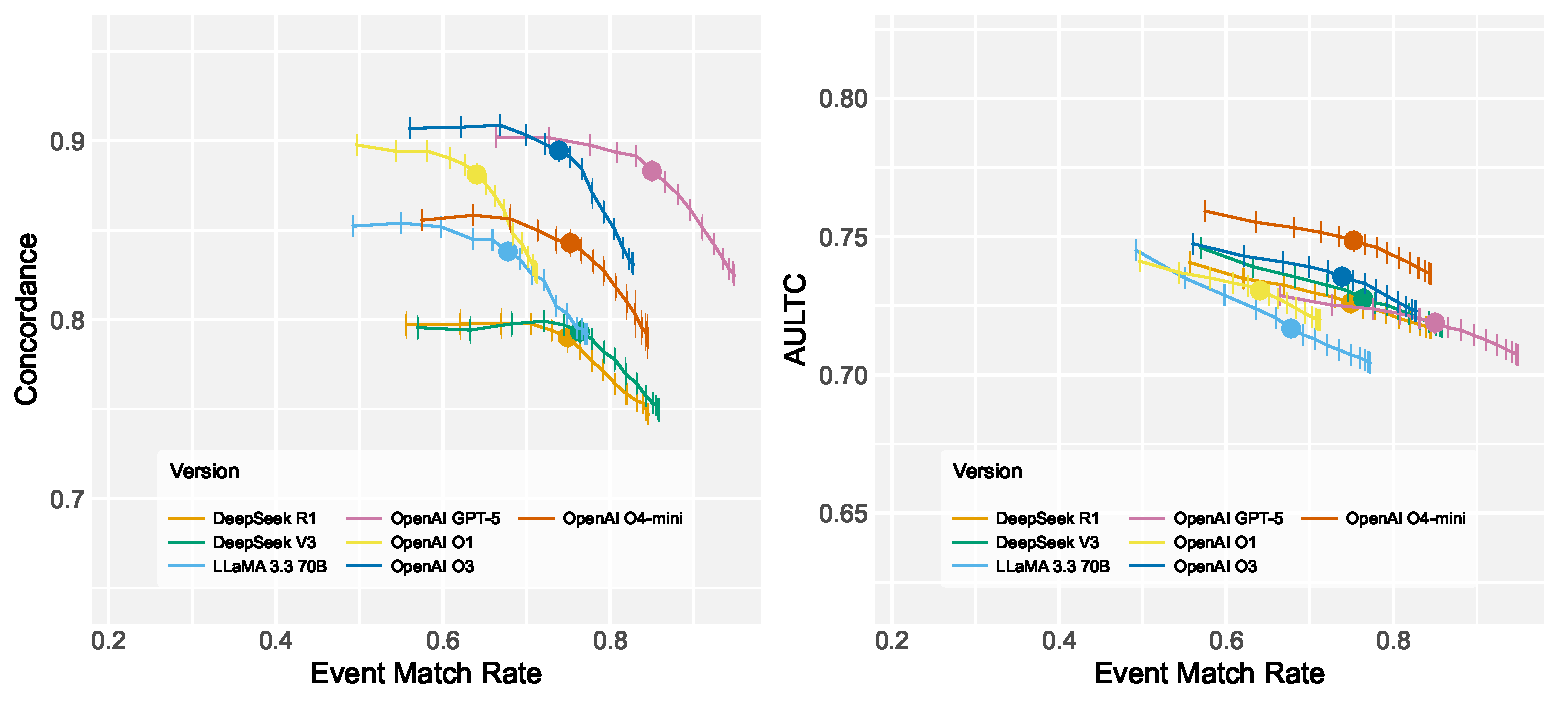
\includegraphics[width=\linewidth]{Appendices/appendix-ch05/images/Scientific_data/Plots_tables/event_match_vs_metrics_lapjv.pdf}
    
    
    

\end{ChFiveFloatBody}
\caption{\textbf{A:} Temporal concordance versus event match rate under LAPJV-based matching.
    \textbf{B:} AULTC versus event match rate. Solid circles ($\bullet$) indicate the operating
    threshold of 0.1; ticks (|) denote 0.01 threshold increments in [0.01, 0.50].}\ChFiveFloatLabel{ch05:fig:threshold_tradeoff_LAPJV}
\end{figure}


Across models, LAPJV preserves high event match rates at low thresholds and exhibits a
smooth trade-off between coverage and temporal accuracy. 
The resulting operating points in Figure~\ref{ch05:fig:threshold_tradeoff_LAPJV}
are highly comparable to those obtained using the recursive matching heuristic in Figure~\ref{ch05:fig:threshold_tradeoff_greedy} (e.g., at $\tau=0.1$, the operating point used in our main results in Table~\ref{ch05:tab:model_comparison}). 
In particular,
the heuristic matcher yields slightly stronger concordance near the elbow of the trade-off
curve, while LAPJV achieves marginally higher AULTC values, reflecting improved timestamp
alignment under global assignment. 
Overall, both strategies lead to consistent qualitative
conclusions.


















% !TeX root = ../../../main.tex
\subsection{Model and Inference Configuration}
\label{ch05:sec:supp-model-configuration}

Seven large language models were evaluated for textual time series annotation:
Llama 3.3 70B Instruct, DeepSeek-R1, DeepSeek-V3, GPT-5, O4-mini, O3,
and O1. The exact checkpoint identifiers and Azure deployment names are
reported in Table~\ref{ch05:tab:model-identifiers}. Llama 3.3 70B Instruct and
DeepSeek-R1 were also used to produce the full-corpus annotations. Each model
was evaluated across five independent generation runs using the textual time
series prompt in Supplementary Section~\ref{ch05:apd:extraction-prompt}. The revised technical-validation
results were calculated on 190 case reports after excluding the 10 pilot cases
used during method development.

Table~\ref{ch05:tab:inference-settings} summarizes the recorded inference
configuration. Llama 3.3 70B Instruct was run using Hugging Face Transformers
and PyTorch with bfloat16 weights and automatic device placement. The Azure
OpenAI models were queried through the Chat Completions interface using API
version \texttt{2024-12-01-preview}. Temperature, top-$p$, and generation seeds
were not explicitly specified for the Azure models. In all API-based runs, the
complete extraction prompt and case-report text were submitted together as a
single user message, and responses were generated without streaming.


% !TeX root = ../../../main.tex
\begin{table}[htbp]
\caption{
Exact model identifiers and Azure OpenAI deployment names used for textual
time series annotation.
}\ChFiveFloatLabel{ch05:tab:model-identifiers}
\ChFiveTableBodyStart
\begin{ChFiveFloatBody}

\centering


\scriptsize
\setlength{\tabcolsep}{6pt}
\renewcommand{\arraystretch}{1.15}
\begin{tabular}{>{\raggedright\arraybackslash}p{0.31\linewidth} >{\raggedright\arraybackslash}p{0.61\linewidth}}
\toprule
\textbf{Model} &
\textbf{Checkpoint identifier or API deployment} \\
\midrule

Llama 3.3 70B Instruct &
\texttt{meta-llama/Llama-3.3-70B-Instruct} \\

DeepSeek-R1 &
\texttt{deepseek-ai/DeepSeek-R1-0528} \\

DeepSeek-V3 &
\texttt{deepseek-ai/DeepSeek-V3-0324} \\

GPT-5 &
Azure OpenAI deployment \texttt{gpt-5} \\

O4-mini &
Azure OpenAI deployment \texttt{o4-mini} \\

O3 &
Azure OpenAI deployment \texttt{o3} \\

O1 &
Azure OpenAI deployment \texttt{o1} \\

\bottomrule
\end{tabular}

\end{ChFiveFloatBody}
\end{table}



% !TeX root = ../../../main.tex
\begin{table}[htbp]
\caption{
Inference and generation settings used for textual time series annotation.
Parameters described as not explicitly set were not supplied in the
corresponding generation request.
}\ChFiveFloatLabel{ch05:tab:inference-settings}
\ChFiveTableBodyStart
\begin{ChFiveFloatBody}

\centering


\scriptsize
\setlength{\tabcolsep}{5pt}
\renewcommand{\arraystretch}{1.18}
\begin{tabular}{
    >{\raggedright\arraybackslash}p{0.18\textwidth}
    >{\raggedright\arraybackslash}p{0.28\textwidth}
    >{\raggedright\arraybackslash}p{0.47\textwidth}
}
\toprule
\textbf{Model or configuration} &
\textbf{Inference framework and precision} &
\textbf{Generation settings} \\
\midrule

Llama 3.3 70B Instruct
(full-corpus annotation) &
Hugging Face Transformers and PyTorch;
bfloat16;
automatic device placement &
128k-token model context;
batch size 1;
\texttt{max\_new\_tokens=8092};
\texttt{do\_sample=True};
\texttt{top\_k=1};
one returned sequence;
temperature and top-$p$ not explicitly set;
no explicit generation seed \\

Llama 3.3 70B Instruct
(technical validation) &
Hugging Face Transformers and PyTorch;
bfloat16;
automatic device placement &
128k-token model context;
batch size 1;
\texttt{max\_new\_tokens=8092};
\texttt{do\_sample=True};
\texttt{temperature=1};
\texttt{top\_k=1};
one returned sequence;
no explicit generation seed \\

DeepSeek-R1 &
DeepSeek-V3 architecture;
checkpoint configuration specifies bfloat16 with FP8 block quantization &
163{,}840-position context;
five independent generation runs using the production textual time series
prompt \\

DeepSeek-V3 &
DeepSeek-V3 architecture;
checkpoint configuration specifies bfloat16 with FP8 block quantization &
163{,}840-position context;
five independent generation runs using the production textual time series
prompt \\

GPT-5 &
Azure OpenAI Chat Completions;
provider-managed numerical precision &
API version \texttt{2024-12-01-preview};
\texttt{max\_completion\_tokens=16834};
\texttt{stream=False};
temperature, top-$p$, and API seed not explicitly set \\

O4-mini, O3, and O1 &
Azure OpenAI Chat Completions;
provider-managed numerical precision &
API version \texttt{2024-12-01-preview};
\texttt{max\_completion\_tokens=40000};
\texttt{stream=False};
temperature, top-$p$, and API seed not explicitly set \\

\bottomrule
\end{tabular}

\end{ChFiveFloatBody}
\end{table}

%%%%%%%%%%%%%%%%%%%%%%%%%%%%%%%%%%%%%%%%%%%
%%%%%%%%%%%%%% Sensitivity analyses %%%%%%%%%%%
%%%%%%%%%%%%%%%%%%%%%%%%%%%%%%%%%%%%%%%%%%





% CH05-SOURCE-END
\clearpage
\endgroup

% !TeX root = ../../main.tex
% Existing source supplement; this is an infrastructure placeholder only.
\appendix{T2S2 CHIL}\label{app:ch06}
% !TeX root = ../../../main.tex
\ProposalPlaceholder{Temporary placeholder for an existing paper appendix or supplement. No supplementary scientific content has been migrated.}


% !TeX root = ../../main.tex
% Existing source supplement; this is an infrastructure placeholder only.
\appendix{T2S2 AAAI}\label{app:ch07}
% !TeX root = ../../../main.tex
\ProposalPlaceholder{Temporary placeholder for an existing paper appendix or supplement. No supplementary scientific content has been migrated.}


% !TeX root = ../../main.tex
% Existing source supplement; this is an infrastructure placeholder only.
\appendix{Textual--Tabular Alignment}\label{app:ch08}
% !TeX root = ../../../main.tex
\ProposalPlaceholder{Temporary placeholder for an existing paper appendix or supplement. No supplementary scientific content has been migrated.}




\urlstyle{rm}
\ifProposalBibliographyReady
  \bibliography{references}
\else
  % Use the template's bibliography heading and required-section tracking.
  % Do not invoke BibTeX on an empty database or fabricate citations.
  \clearpage
  \bibsection
  \ProposalPlaceholder{The unified bibliography will be populated from the selected manuscripts during their approved migrations.}
\fi
\tagstructend
\end{document}
